% ACL-format version (review mode, double-blind) of the 385M English-to-African translation paper.
% Style: official acl.sty / acl_natbib.bst (acl-org/acl-style-files, copy taken from a local checkout of the official sources).
% Compiles with pdfLaTeX (Overleaf default), XeLaTeX and LuaLaTeX. Bibliography: BibTeX with acl_natbib.
% Core = title ... Conclusion (hard limit 8 pages); Limitations, Ethical considerations, references and appendix are outside the core.
% Numbers come from paper_385m/paper.md only; claim IDs of CLAIMS_LEDGER.md are kept as % comments.
% [VERIFY ...] / [PENDING ...] marks are deliberate and listed in OPEN_ISSUES.md.
\documentclass[11pt]{article}
% Two builds from the same sources:
%   main.tex          review build (anonymous, line numbers, no author, no links that identify the authors)
%   main_preprint.tex preprint build (\def\preprintbuild before % ACL-format version (review mode, double-blind) of the 385M English-to-African translation paper.
% Style: official acl.sty / acl_natbib.bst (acl-org/acl-style-files, copy taken from a local checkout of the official sources).
% Compiles with pdfLaTeX (Overleaf default), XeLaTeX and LuaLaTeX. Bibliography: BibTeX with acl_natbib.
% Core = title ... Conclusion (hard limit 8 pages); Limitations, Ethical considerations, references and appendix are outside the core.
% Numbers come from paper_385m/paper.md only; claim IDs of CLAIMS_LEDGER.md are kept as % comments.
% [VERIFY ...] / [PENDING ...] marks are deliberate and listed in OPEN_ISSUES.md.
\documentclass[11pt]{article}
% Two builds from the same sources:
%   main.tex          review build (anonymous, line numbers, no author, no links that identify the authors)
%   main_preprint.tex preprint build (\def\preprintbuild before % ACL-format version (review mode, double-blind) of the 385M English-to-African translation paper.
% Style: official acl.sty / acl_natbib.bst (acl-org/acl-style-files, copy taken from a local checkout of the official sources).
% Compiles with pdfLaTeX (Overleaf default), XeLaTeX and LuaLaTeX. Bibliography: BibTeX with acl_natbib.
% Core = title ... Conclusion (hard limit 8 pages); Limitations, Ethical considerations, references and appendix are outside the core.
% Numbers come from paper_385m/paper.md only; claim IDs of CLAIMS_LEDGER.md are kept as % comments.
% [VERIFY ...] / [PENDING ...] marks are deliberate and listed in OPEN_ISSUES.md.
\documentclass[11pt]{article}
% Two builds from the same sources:
%   main.tex          review build (anonymous, line numbers, no author, no links that identify the authors)
%   main_preprint.tex preprint build (\def\preprintbuild before % ACL-format version (review mode, double-blind) of the 385M English-to-African translation paper.
% Style: official acl.sty / acl_natbib.bst (acl-org/acl-style-files, copy taken from a local checkout of the official sources).
% Compiles with pdfLaTeX (Overleaf default), XeLaTeX and LuaLaTeX. Bibliography: BibTeX with acl_natbib.
% Core = title ... Conclusion (hard limit 8 pages); Limitations, Ethical considerations, references and appendix are outside the core.
% Numbers come from paper_385m/paper.md only; claim IDs of CLAIMS_LEDGER.md are kept as % comments.
% [VERIFY ...] / [PENDING ...] marks are deliberate and listed in OPEN_ISSUES.md.
\documentclass[11pt]{article}
% Two builds from the same sources:
%   main.tex          review build (anonymous, line numbers, no author, no links that identify the authors)
%   main_preprint.tex preprint build (\def\preprintbuild before \input{main}): author block, live Hugging Face links, page numbers
\ifdefined\preprintbuild
  \usepackage[preprint]{acl}
\else
  \usepackage[review]{acl}   % camera-ready: \usepackage[final]{acl}
\fi
\newif\ifanon \anontrue
\ifdefined\preprintbuild \anonfalse \fi
\usepackage{iftex}
\ifPDFTeX
  \usepackage{times}
  \usepackage{latexsym}
  \usepackage[T1]{fontenc}
  \usepackage[utf8]{inputenc}
  \usepackage{inconsolata}
\else
  \usepackage{fontspec} % XeLaTeX/LuaLaTeX only
  \setmainfont{texgyretermes}[Extension=.otf,UprightFont=*-regular,BoldFont=*-bold,ItalicFont=*-italic,BoldItalicFont=*-bolditalic]
  \setmonofont{texgyrecursor}[Extension=.otf,UprightFont=*-regular,BoldFont=*-bold,ItalicFont=*-italic,BoldItalicFont=*-bolditalic,Scale=0.9]
\fi
\usepackage{microtype}
\usepackage{booktabs,array,tabularx,longtable,graphicx,amsmath,amssymb,enumitem,placeins,etoolbox}
\usepackage{adjustbox}
\usepackage{tikz}
\usetikzlibrary{positioning,arrows.meta}
\usepackage{pgfplots}\pgfplotsset{compat=1.16}
\pretocmd{\section}{\FloatBarrier}{}{}
\setlist{itemsep=0pt,topsep=2pt,parsep=0pt,leftmargin=*}
\renewcommand{\arraystretch}{1.05}
\setlength{\textfloatsep}{8pt plus 2pt minus 2pt}
\setlength{\floatsep}{6pt plus 2pt minus 2pt}
\setlength{\intextsep}{6pt plus 2pt minus 2pt}
\setlength{\dbltextfloatsep}{8pt plus 2pt minus 2pt}
\captionsetup{font=small,skip=3pt}
\input{macros}

\title{What Does Reinforcement Learning Add to a Small Translator for African Languages?}
\ifanon
  \author{Anonymous ACL submission}
\else
  \author{Jeffrey Otoibhi \\ Aletheia AI \\ \textit{[Co-authors to be added]}}
\fi

\begin{document}
\maketitle
\begin{abstract}
\input{sections/abstract}
\end{abstract}
\input{sections/s1_intro}
\input{sections/s2_related}
\input{sections/s3_method}
\input{sections/s4_eval}
\input{sections/s5_results}
\input{sections/s6_discussion}
\FloatBarrier\label{coreend}
\clearpage
\section*{Limitations}
\input{sections/limitations}
\section*{Ethical considerations}
\input{sections/ethics}
\ifanon\else
\section*{Author contributions}
\textit{[Placeholder, to be filled by the lead author: one sentence per person describing what that person contributed (for example design, data, training, evaluation, writing). Authorship is based on contribution.]}
\fi
\bibliography{refs}
\bibliographystyle{acl_natbib}

\clearpage
\appendix
\label{appstart}
\onecolumn
\input{sections/appendix}
\end{document}
): author block, live Hugging Face links, page numbers
\ifdefined\preprintbuild
  \usepackage[preprint]{acl}
\else
  \usepackage[review]{acl}   % camera-ready: \usepackage[final]{acl}
\fi
\newif\ifanon \anontrue
\ifdefined\preprintbuild \anonfalse \fi
\usepackage{iftex}
\ifPDFTeX
  \usepackage{times}
  \usepackage{latexsym}
  \usepackage[T1]{fontenc}
  \usepackage[utf8]{inputenc}
  \usepackage{inconsolata}
\else
  \usepackage{fontspec} % XeLaTeX/LuaLaTeX only
  \setmainfont{texgyretermes}[Extension=.otf,UprightFont=*-regular,BoldFont=*-bold,ItalicFont=*-italic,BoldItalicFont=*-bolditalic]
  \setmonofont{texgyrecursor}[Extension=.otf,UprightFont=*-regular,BoldFont=*-bold,ItalicFont=*-italic,BoldItalicFont=*-bolditalic,Scale=0.9]
\fi
\usepackage{microtype}
\usepackage{booktabs,array,tabularx,longtable,graphicx,amsmath,amssymb,enumitem,placeins,etoolbox}
\usepackage{adjustbox}
\usepackage{tikz}
\usetikzlibrary{positioning,arrows.meta}
\usepackage{pgfplots}\pgfplotsset{compat=1.16}
\pretocmd{\section}{\FloatBarrier}{}{}
\setlist{itemsep=0pt,topsep=2pt,parsep=0pt,leftmargin=*}
\renewcommand{\arraystretch}{1.05}
\setlength{\textfloatsep}{8pt plus 2pt minus 2pt}
\setlength{\floatsep}{6pt plus 2pt minus 2pt}
\setlength{\intextsep}{6pt plus 2pt minus 2pt}
\setlength{\dbltextfloatsep}{8pt plus 2pt minus 2pt}
\captionsetup{font=small,skip=3pt}
% Macros for the 385M paper.
\newcommand{\chrfpp}{chrF++}
\newcommand{\ci}[2]{\mbox{$[#1,\,#2]$}}          % interval, e.g. \ci{+8.59}{+9.03}
\newcommand{\tool}[1]{\texttt{#1}}
\newcommand{\verify}[1]{\textbf{[VERIFY: #1]}}   % unsettled fact, listed in OPEN_ISSUES.md
\newcommand{\verifycite}[1]{\textbf{[VERIFY citation: #1]}} % claim stated without citation
\newcommand{\pending}[1]{\textbf{[PENDING: #1]}} % result not yet in
\newcommand{\ownerdecision}[1]{\textbf{[OWNER: #1]}}
\newcommand{\GPUh}{A100-h}
% Build switch: \ifanon is true in the review build (main.tex) and false in the preprint build (main_preprint.tex).
\newcommand{\anonreal}[2]{\ifanon #1\else #2\fi}   % #1 printed in the anonymous build, #2 in the preprint build


\title{What Does Reinforcement Learning Add to a Small Translator for African Languages?}
\ifanon
  \author{Anonymous ACL submission}
\else
  \author{Jeffrey Otoibhi \\ Aletheia AI \\ \textit{[Co-authors to be added]}}
\fi

\begin{document}
\maketitle
\begin{abstract}
% [abstract numbers: R1, R4-R6, R8, R19-R20, N2, W4, SC3, DL1-DL3, E01, E02, E03, E04, E11; every number is repeated in the body]
We grow Gemma-3-270m into a 385M-parameter English-to-African translator with 125 single-token language tags, fine-tune it on decontaminated data (SFT) and apply GRPO with reference-free quality-estimation (QE) rewards. RL raises FLORES+ devtest \chrfpp{} from 22.85 to 31.66 ($+8.81$, 95\% CI \ci{+8.59}{+9.03}, 54 languages); every language improves. About half of this is finishing and looping: a decode-time frequency penalty of 0.10 on the SFT, chosen by a rule fixed in advance, recovers 49\% of the \chrfpp{} gain without RL; RL still adds $+4.37$ \ci{+4.28}{+4.46} \chrfpp{} on top of the guarded SFT and stays $+1.60$ \ci{+1.34}{+1.88} ahead of the best decoded SFT. Of the gain up to the second RL stage, 94\% arrives in the first; the next step ($+0.31$) is not separable from seed noise (two extra seeds differ by 0.06 \ci{-0.02}{+0.14}). On the 43 languages shared with the published NLLB-200 table, the 385M model reaches 92\% of the \chrfpp{} of NLLB-3.3B (35.54 against 38.80; NLLB-3.3B has about 8.6 times the parameters) and matches or beats it on 7 of 43. A matched-compute control, continued SFT for the GPU time of the RL chain, has the pre-registered verdict ``inconclusive'': RL minus control is $+4.58$ \ci{+4.45}{+4.70} over 93 benchmark-language cells, but $-0.03$ \ci{-0.13}{+0.09} on the 19 languages that have teacher-translated data and $+9.29$ on the other 46 cells. The reward's own loop flag undercounts degeneration by a factor of 1.77. In science translation the science SFT, not the science RL, carries the gain: the same RL started without it ends 1.44 chrF \ci{1.25}{1.61} lower. One training seed per model; all scoring is automatic.

\end{abstract}
\section{Introduction}\label{sec:intro}
A small translator for many African languages fails mostly by not stopping (unfinished or looping output), by copying the source and by writing the wrong language. Supervised fine-tuning (SFT) leaves these failures in place: on FLORES+ devtest our 385M SFT finishes 0.829 of its outputs, loops in 0.209 and writes 3.03 times the reference length. We grow Gemma-3-270m to 385M parameters, fine-tune it on decontaminated data for 125 languages and apply GRPO with reference-free quality-estimation (QE) rewards. Our question is what RL adds beyond what a cheaper tool already gives, and we answer it with controls rather than with a larger gain.
% [R1-R8, R19-R20, N2, W4, SC3, DL1-DL3]

\textbf{Findings.} (i) RL improves every FLORES+ language ($+8.81$ \chrfpp{}). (ii) About half of the gain is finishing and looping; a one-line decode-time frequency penalty on the SFT recovers 49\% without RL, and RL still adds $+4.37$ \chrfpp{} (Section~\ref{sec:rlsft}). (iii) Most of the gain arrives in the first RL stage; later stages add little (Section~\ref{sec:seeds}). (iv) The reward's loop flag undercounts degeneration by 1.77 (Section~\ref{sec:degen}). (v) A matched-compute continued-SFT control has the registered verdict ``inconclusive'' (Section~\ref{sec:control}).

\textbf{Not claimed.} We do not claim that RL is in general a better use of compute than SFT; that the finishing gap is a property of RL rather than of unguarded greedy decoding; that any reward component beyond four stage-A features helps; that the model beats NLLB-3.3B, a model with about 8.6 times the parameters (it is 3.26 \chrfpp{} below it on 43 shared languages); that it beats our earlier 270M model; or any ``first''. All scoring is automatic.

\textbf{Contributions.} (1) A decomposition of an RL gain into finishing/looping and translation quality with decode-time, beam/MBR and matched-compute controls, a metric-independence rule and an independent audit of the reward's loop flag. (2) A decontaminated SFT/RL pipeline for 125 languages with a training-text audit. (3) Negative results (weak-group RL, science SFT on the headline metric, whole-document decoding). Artefacts: \anonreal{anonymised for review; released on acceptance}{model weights at \url{https://huggingface.co/AletheiaAING/gemma-0.4B-translate-rl} (details in Ethical considerations)}.

\section{Related Work}\label{sec:related}
% Adapted from the earlier related-work review; only works in the bib files are cited.
\textbf{African MT.} Community infrastructure and benchmarks include Masakhane \citep{nekoto2020participatory}, MAFAND-MT \citep{adelani2022mafand}, FLORES-200 and NLLB-200 \citep{goyal2022flores101,nllb2022nllb}, FLORES+ \citep{oldi2025floresplus}, NTREX-128 \citep{federmann2022ntrex}, SALT \citep{akera2022salt}, SMOL \citep{caswell2025smol} and AfriScience-MT, which reports SSA-COMET \citep{li2025ssacomet} as its primary metric \citep{abdulmumin2026afriscience}. Larger African-language LLMs include AfriqueLLM \citep{yu2026afriquellm}; TranslatePsy-AfriSLM \citep{gritta2026translatepsy} is the nearest small-model competitor.

\textbf{RL for MT.} GRPO \citep{shao2024deepseekmath,yu2025dapo} underlies R1-style MT work \citep{feng2025mtr1zero,wang2025deeptrans,cheng2025seedx,zheng2025hunyuanmt}; TranslateGemma uses a reward-model ensemble on Gemma 3 at 4B and up \citep{finkelstein2026translategemma}. Closest to us are RL on NLLB with round-trip chrF++ \citep{attia2026roundtrip}, reference-free GRPO on NLLB \citep{garciaestrada2026reffree}, chrF rewards for unseen languages \citep{hu2026rlunseen}, QE-reward hacks \citep{liu2026walar} and language-ID-gated QE rewards \citep{han2026milmmtrl}. Minimum Bayes risk and quality-aware decoding \citep{freitag2022mbr,fernandes2022qualityaware} compete for many of the same gains. Whether RL generalises where SFT memorises \citep{chu2025sft} or only sharpens \citep{yue2025doesrl} has been asked for reasoning; we searched for a matched-compute SFT-versus-RL comparison for translation and found none (the nearest, reference-free GRPO on NLLB against three epochs of supervised fine-tuning, does not match GPU time \citep{garciaestrada2026reffree}).

\textbf{Metrics and reward hacking.} AfriCOMET \citep{wang2024africomet}, SSA-COMET, chrF++ and sacreBLEU \citep{popovic2017chrfpp,post2018call}, paired bootstrap \citep{koehn2004significance}; learned rewards are overoptimised \citep{gao2023scaling,coste2024ensembles}; GlotLID \citep{kargaran2023glotlid} covers language identification. We claim no priority for RL in MT, small models or language coverage.

\section{Approach}\label{sec:method}
% [M1-M11 L1-L4 CT1-CT3 R9 R10 W6 SC1 DL4] Internal stage names are explained in Appendix~\ref{app:glossary}.
Figure~\ref{fig:overview} shows the pipeline. We describe the model and the two training steps, then the variants used as controls and extensions.

\begin{figure*}[t]
\centering
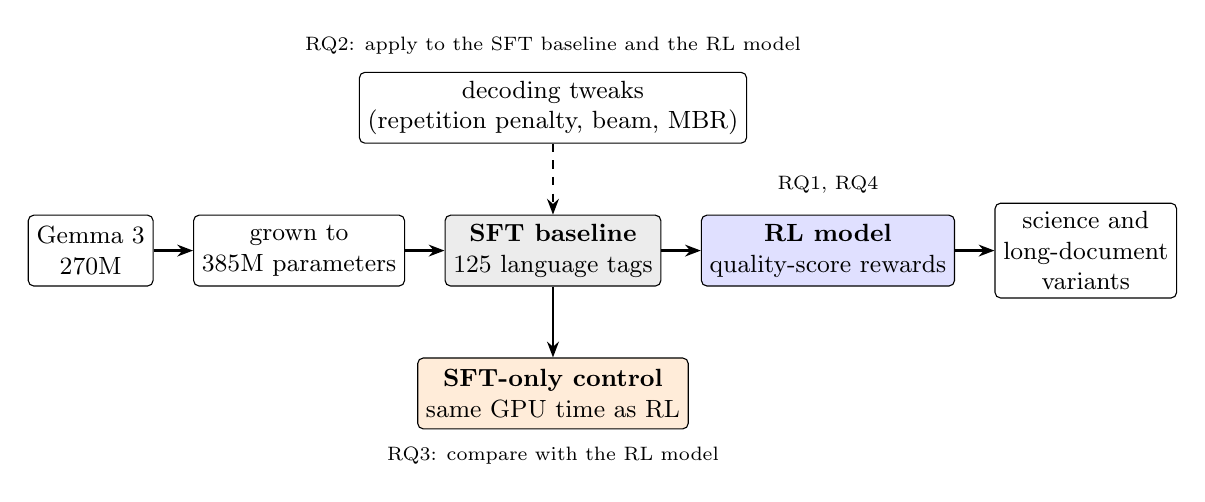
\begin{tikzpicture}[font=\small, node distance=5mm, box/.style={draw, rounded corners=2pt, align=center, minimum height=9mm, inner sep=3pt}, arr/.style={-{Stealth[length=2mm]}, thick}, lab/.style={font=\scriptsize, align=center}]
\node[box] (g) {Gemma 3\\ 270M};
\node[box, right=of g] (grow) {grown to\\ 385M parameters};
\node[box, right=of grow, fill=gray!15] (sft) {\textbf{SFT baseline}\\ 125 language tags};
\node[box, right=of sft, fill=blue!12] (rl) {\textbf{RL model}\\ quality-score rewards};
\node[box, right=of rl] (sci) {science and\\ long-document\\ variants};
\node[box, below=9mm of sft, fill=orange!15] (ctl) {\textbf{SFT-only control}\\ same GPU time as RL};
\node[box, above=9mm of sft] (dec) {decoding tweaks\\ (repetition penalty, beam, MBR)};
\draw[arr] (g) -- (grow); \draw[arr] (grow) -- (sft); \draw[arr] (sft) -- (rl); \draw[arr] (rl) -- (sci);
\draw[arr] (sft) -- (ctl); \draw[arr, dashed] (dec) -- (sft);
\node[lab, below=1mm of ctl] {RQ3: compare with the RL model};
\node[lab, above=1mm of dec] {RQ2: apply to the SFT baseline and the RL model};
\node[lab, above=1.5mm of rl] {RQ1, RQ4};
\end{tikzpicture}
\caption{Overview. A 270M model is grown to 385M parameters and fine-tuned (the SFT baseline), then trained with reinforcement learning (the RL model). Two controls ask what else could give the same gain: decoding changes (RQ2) and more fine-tuning for the same GPU time (RQ3).}\label{fig:overview}
\end{figure*}

\textbf{Model.} We start from Gemma-3-270m-it \citep{gemmateam2025gemma3} and add layers to reach 385M parameters (39 layers) \citep[cf.][]{wu2024llamapro,kim2023solar}. The task is English to one of 125 languages. A single extra token in the vocabulary names the target language, and the model answers with that token followed by the translation.

\textbf{Step 1: supervised fine-tuning (the SFT baseline).} We train on English-to-African sentence pairs and instruction data. Before training, we remove every pair that matches the text of any benchmark we later use, checked on both sides of the pair. Part of the data comes from NLLB-mined sentences and a collection of translated instructions; we report their share and licences in the Ethical considerations. Training uses the Muon optimiser \citep{liu2025muon} and takes about 45 hours on one A100 GPU (Appendix~\ref{app:hyper}).

\textbf{Step 2: reinforcement learning (the RL model).} We use GRPO \citep{shao2024deepseekmath}. For each English text the model samples 16 translations. Each translation receives a reward, and the model is nudged towards translations that score above the average of their group and away from those below it; a penalty keeps the model close to its starting point. Three stages follow one another, and the first does most of the work (Section~\ref{sec:rq4}). The reward has three parts. (i) A translation that fails a hard check scores the minimum: wrong or missing language tag, no end of text, a copy of the input, repetition, the wrong language, or an implausible length. (ii) Otherwise a quality score without a reference translation rates the output. We combine two quality models \citep{wang2024africomet,li2025ssacomet}, taking their mean unless they disagree strongly, and for languages without a validated quality model we reward agreement with the group's other samples. (iii) Small penalties discourage, among other things, unusual length, missing numbers or names, and missing diacritics. Exact settings are in Appendix~\ref{app:hyper}.

\textbf{Variants.} The \emph{SFT-only control} continues SFT from the baseline for the same GPU time as the RL stages, using half replay data and half extra English-to-X pairs for 19 languages \citep{gritta2026translatepsy}. The \emph{science variant} adds a short fine-tuning step on science text from AfriScience-MT \citep{abdulmumin2026afriscience} and then a second RL run; the \emph{long-document variant} adds RL on long inputs. Internal names used in the appendix tables are listed in Appendix~\ref{app:glossary}.

\section{Experimental Setup}\label{sec:eval}
% [M11 CT1-CT6 X1 X2 X5 X7 X9]
\textbf{Benchmarks.} We translate English into African languages on the standard FLORES+ devtest set \citep{oldi2025floresplus} (1,012 sentences; 54 languages), NTREX-128 \citep{federmann2022ntrex} (24 languages) and MAFAND-MT \citep{adelani2022mafand} (15 languages). Smaller sets, SmolSent \citep{caswell2025smol}, SALT \citep{akera2022salt}, GlotStoryBook \citep{kargaran2023glotlid}, IbomMT \citep{kalejaiye2025ibom} and FLORES-MOZ \citep{moznlp2026floresmoz}, appear in the appendix, as does AfriScience-MT \citep{abdulmumin2026afriscience} for science text. Unless stated, we report the average over languages, with each language counting equally.

\textbf{Metrics.} \emph{chrF++} compares character and word n-grams of the output with a human reference; higher is better. \emph{Held-out AfriCOMET} is a learned score that compares source, output and reference; we never use it as a reward. The \emph{finished rate} is the share of outputs that end properly; the \emph{loop rate} is the share that repeat themselves. Both are the checks our reward also uses, so they are not independent evidence of better translation. We computed chrF++ with sacreBLEU 2.6.0 (word order 2, otherwise defaults) after Unicode normalisation; the full signature string was not saved.

\textbf{Avoiding self-deception.} First, \emph{independence}: the metrics inside the reward (the two quality models, agreement between samples, and the finished, repetition and language checks) are not evidence that RL helped. Our evidence is chrF++ and held-out AfriCOMET against human references (Appendix~\ref{app:indep}). Second, \emph{paired tests}: every difference is a paired bootstrap over test sentences with a 95\% interval, which covers sentence variance but not training randomness. Third, \emph{contamination}: besides filtering the training pairs, we scanned 26 million training samples against all benchmark text and found no benchmark sentence of three or more words (Ethical considerations list the residuals). Fourth, \emph{seeds}: every model is one training run; we measured seed noise only for the first RL stage on 20 languages.

\textbf{Decoding.} All main results use greedy decoding with up to 768 new tokens (vLLM, bf16). The \emph{repetition penalty} used as a control is a decoding setting that discourages repeated tokens; we chose its strength on a development set by a rule fixed in advance. Beam search and MBR decoding are described where they appear.

\section{Results}\label{sec:results}

\subsection{RL against SFT, and what a decode-time guard recovers}\label{sec:rlsft}
% [R1 R2 R3 R4 R5 R6 R13 D5; EVID tables 1-2; E01] GATE E-01
``SFT'' is the 385M SFT final; ``RL'' is the final general RL model (mixed-stage best); 214 rows flagged by the contamination audit are removed. RL improves \chrfpp{} on every benchmark (Table~\ref{tab:headline}); plain chrF over the 93 cells improves by $+8.59$ \ci{+8.43}{+8.76} and held-out AfriCOMET (76 cells) by $+0.0631$ \ci{+0.0620}{+0.0643}. All 54 FLORES+ and 24 NTREX languages improve on \chrfpp{}, chrF and AfriCOMET with intervals above zero; on MAFAND-MT 14 of 15 improve (pcm $-0.25$ \ci{-0.69}{+0.30}).

\begin{table}[t]
\centering\footnotesize\setlength{\tabcolsep}{2pt}
\caption{RL against SFT (language-macro \chrfpp{}, clean rows, 95\% paired bootstrap, one seed).}\label{tab:headline}
\begin{tabular}{@{}lrrl@{}}
\toprule
benchmark (n) & SFT & RL & RL $-$ SFT\\
\midrule
FLORES+ (54) & 22.85 & 31.66 & $+8.81$ \ci{+8.59}{+9.03}\\
NTREX (24) & 29.25 & 37.17 & $+7.91$ \ci{+7.69}{+8.12}\\
MAFAND-MT (15) & 35.77 & 40.78 & $+5.01$ \ci{+4.76}{+5.23}\\
all 93 cells & 26.59 & 34.55 & $+7.96$ \ci{+7.82}{+8.12}\\
\bottomrule
\end{tabular}
\end{table}

\textbf{Finishing and looping.} On FLORES+ (finished / loop / hypothesis-to-reference length) the SFT has 0.829 / 0.209 / 3.03, RL stage A 0.983 / 0.068 / 1.33 and the mixed best 0.995 / 0.048 / 1.14 (Appendix~\ref{app:rlsft}). Cutting the SFT's looping outputs at the loop onset, without changing the translation, lifts the SFT from 26.59 to 30.49 \chrfpp{}: \textbf{49\% of the gain is recovered by cutting loops}. 67 to 70\% of the gain sits in rows where either model failed, and about 41\% of the AfriCOMET gain is finishing. On rows where the SFT finished and did not loop, RL is still $+2.41$ \ci{+2.33}{+2.49} \chrfpp{} and $+0.0366$ AfriCOMET ahead, significant in 50 of 54 FLORES+ languages; the estimates favour different models and agree in sign and rough size.

\textbf{Decode-time loop guard (E-01).} Greedy decoding with a vLLM frequency penalty of 0.10 (best of a seven-setting dev grid; plain greedy 34.50, best 37.36 dev \chrfpp{}) gives SFT $26.59\to30.48$ and RL $34.55\to34.84$ \chrfpp{} over the 93 cells, and AfriCOMET (76 cells) SFT $0.565\to0.583$, RL $0.628\to0.631$ (Figure~\ref{fig:decomp}). \textbf{A guard on the SFT recovers the same 49\% of the \chrfpp{} gain (29\% of the AfriCOMET gain) without RL}; RL with the guard minus SFT with the guard is $+4.37$ \ci{+4.28}{+4.46} \chrfpp{} and $+0.0479$ \ci{+0.0469}{+0.0490} AfriCOMET ($+2.63$ \ci{+2.56}{+2.70} \chrfpp{} on rows where the guarded SFT is clean). Caveats: the optimum (0.10) lies at the edge of the grid, so the control may be under-tuned; a post-hoc dev-only extension was still rising (SFT dev \chrfpp{} 37.36 at 0.10, 37.97 at 0.20, 38.00 at 0.30, 38.25 at 0.50) and no full evaluation with a stronger penalty was run; one seed. With the guard, FLORES+ zgh and MAFAND-MT pcm are significantly worse for RL than for the SFT.

\begin{figure*}[t]
\centering
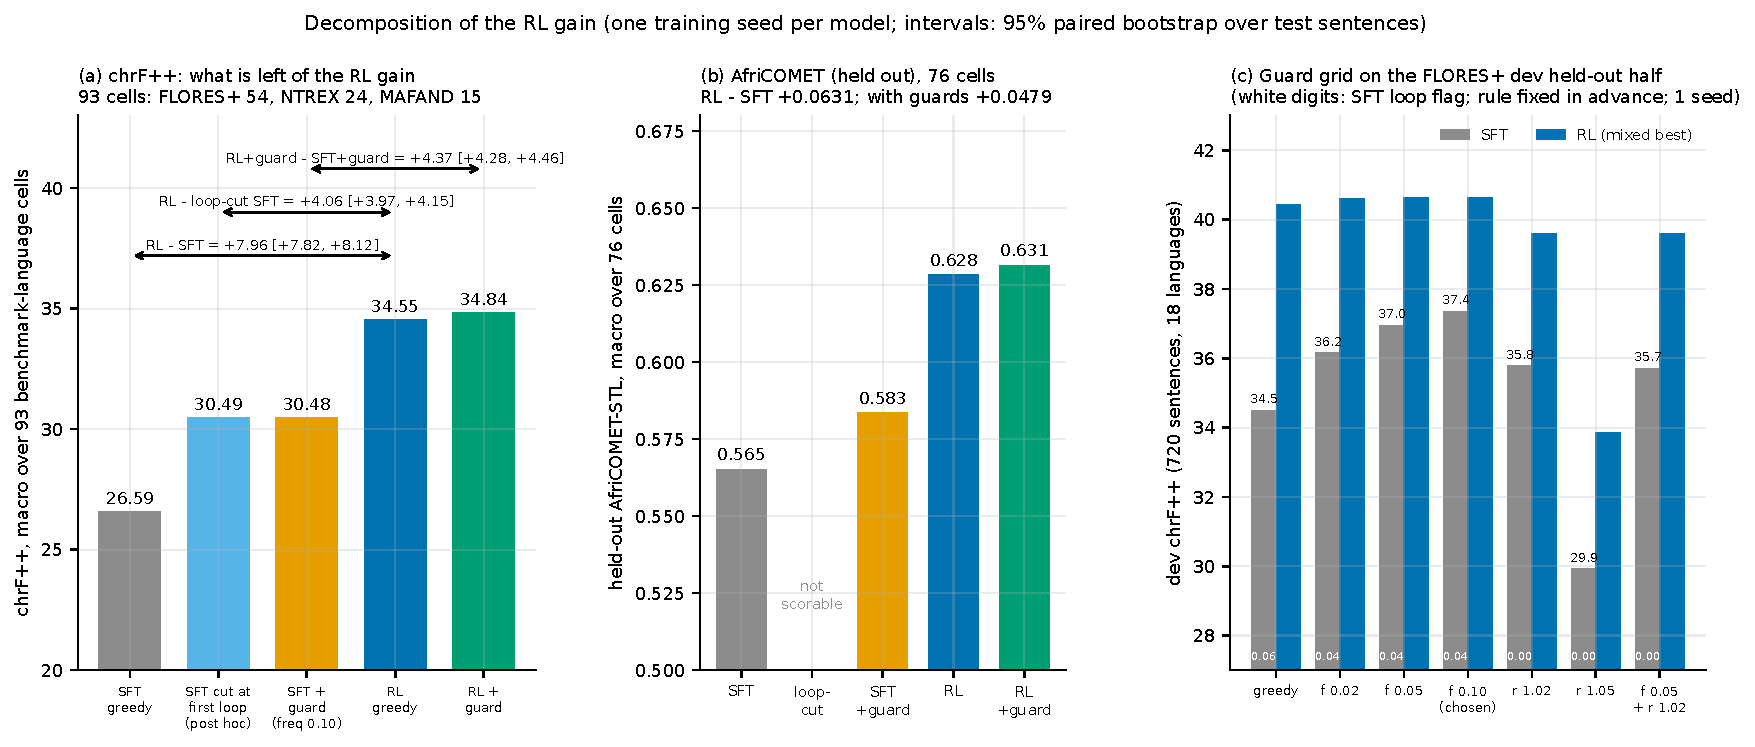
\includegraphics[width=\textwidth]{figures/fig3_decomposition_guard.pdf}
\caption{Decomposition of the RL gain with the decode-time guard (E-01). (a) Language-macro \chrfpp{} over 93 cells: SFT 26.59, SFT cut at its first loop 30.49 (post hoc), SFT with frequency penalty 0.10 30.48, RL 34.55, RL with guard 34.84; arrows give paired differences with 95\% CI. (b) Held-out AfriCOMET over 76 cells. (c) The seven-setting guard grid on the FLORES+ dev held-out half (720 sentences, 18 languages); the optimum (0.10) lies at the edge of the grid. One seed per model.}\label{fig:decomp}
\end{figure*}

\textbf{Growth and the earlier model.} The 385M SFT is significantly better than A0 on seven of eight benchmarks (FLORES+ $+5.31$ \ci{+5.13}{+5.50}, 46 languages; the comparison confounds depth with the extra stage-B SFT). In the same harness, on rows clean for both generations (E-13), it is behind our earlier 270M SFT on FLORES+ ($-2.35$ \ci{-3.25}{-1.38}), NTREX ($-4.13$) and MAFAND-MT ($-3.54$); after RL it is level on FLORES+ ($+0.35$ \ci{+0.08}{+0.62}) and NTREX ($+0.02$ \ci{-0.07}{+0.11}) and $1.55$ \chrfpp{} lower on MAFAND-MT, with data, steps, tokenizer layout and reward differing and only 4.7\% of FLORES+ rows kept (Appendix~\ref{app:sft}).

\subsection{Independent audit of the loop flag}\label{sec:degen}
% [R19-R24 DEGEN]
The reward's loop flag is the guard the RL was optimised against, so a missed loop type would be undercounted for RL. We re-measured with a detector sharing the idea but none of the code or constants (lzma-compressed size relative to human references of the same benchmark, language and length; repeated character 8-grams; repeated word 3-grams; each threshold set so that 0.1\% of 122,585 human references fire it). \textbf{The reward's flag is a lower bound:} on mixed-best FLORES+ the independent detector flags 1.77 \ci{1.71}{1.84} times as many outputs (0.0851 against 0.0480; SFT 0.3107 against 0.2095, ratio 1.48). The extra rows are finished partial repetitions: if they scored the average of their language's unflagged rows, mixed-best macro \chrfpp{} would rise by at most 0.19 (FLORES+), against 0.46 for the SFT, so the decomposition changes by 3.0\% to 4.4\% of the RL gains at most. Two further findings: 24.5\% of the 2,079 mixed-best rows above twice the reference length are flagged by neither detector, and \textbf{English output rises in the Arabic dialects and Tamazight} (aeb 0.215 to 0.449, ary 0.041 to 0.394, arz 0.006 to 0.098, zgh 0.001 to 0.049, SFT to mixed best; languages outside the RL prompt pool), so part of ``RL loops less'' there is a change from loops to English, while their \chrfpp{} stays at 2 to 9 (Appendix~\ref{app:degenapp}).

\begin{figure*}[t]
\centering
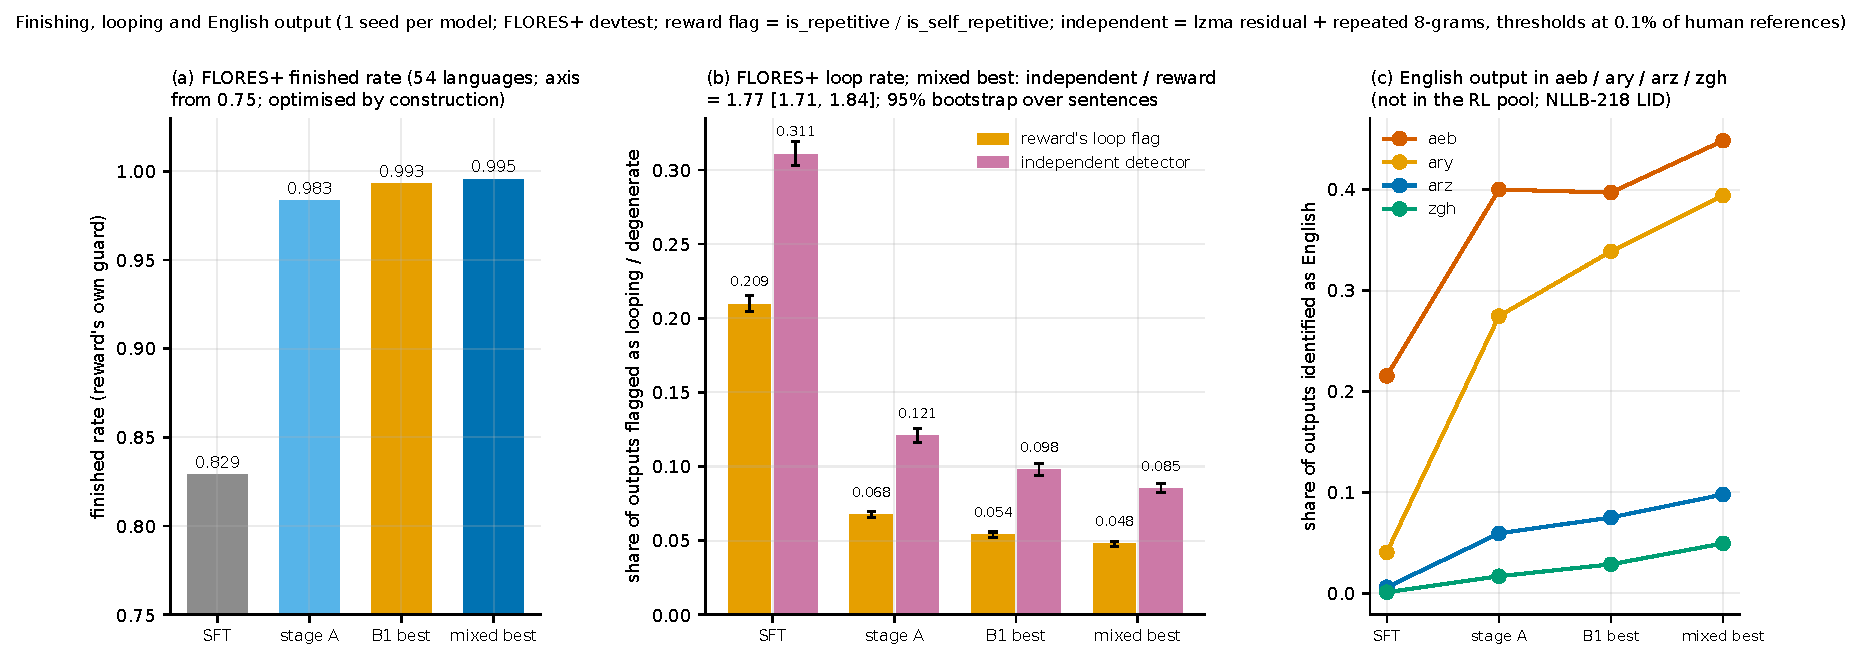
\includegraphics[width=\textwidth]{figures/fig7_loops_finishing.pdf}
\caption{Finishing, looping and English output on FLORES+ devtest (language macro, one seed per model). (a) Finished rate (54 languages; axis from 0.75). (b) Reward loop flag against the independent detector; error bars 95\% bootstrap over source sentences. (c) Share of outputs identified as English (NLLB-218 LID, $p\ge0.5$) in four languages outside the RL prompt pool.}\label{fig:loops}
\end{figure*}

\subsection{Where the gain accrues; seeds and ablations}\label{sec:seeds}
% [R8 E04 E11 M10 R17 R18]
Stage A gives 94\% of the SFT-to-B1 gain on FLORES+ (7.96 of 8.50); B1 adds $+0.54$ \ci{+0.49}{+0.59} and the mixed stage $+0.31$ \ci{+0.26}{+0.35} (NTREX $+0.30$, $+0.18$; MAFAND-MT nothing). B1 final (step 135) equals B1 best within noise. \textbf{Seeds (E-04).} Two extra runs of the stage-A recipe (100 steps, 20 languages, 49 cells) gain $+5.96$ \ci{+5.80}{+6.11} and $+5.90$ \ci{+5.74}{+6.05} \chrfpp{} over the SFT; they differ by \textbf{0.06} \ci{-0.02}{+0.14}. On those languages B1 best is $+0.17$ \ci{+0.12}{+0.21} over stage A, about three times the seed difference, while the mixed step is $+0.07$ \ci{+0.02}{+0.11}, the size of the seed difference: \textbf{we do not call the mixed step a gain}. This is one pair of seeds at step 100, not a seed study of later stages. RL aimed at eight weak West-African languages (85 steps, MBR guide) adds $+0.03$ \ci{-0.06}{+0.12} on its targets against a pre-registered $+1.0$ (negative result).

\textbf{Ablations (E-11).} One run per arm, 100 steps, forks of seed 2's step-40 state (Figure~\ref{fig:seeds}). Removing all four stage-A features costs \textbf{0.32} \ci{0.23}{0.41} \chrfpp{} (about 5\% of the gain, five times the seed difference); removing the reference domain costs 0.16 \ci{0.08}{0.25}; removing the beam guide costs 0.09 against seed 2 but $0.04$ \ci{-0.04}{+0.11} against seed 3, \textbf{not separable from seed noise}, for 25\% more step time. The KL rise is not caused by the features (median KL of steps 81 to 90: 0.116 without any feature, 0.120 to 0.123 in the other arms). The features are design choices with a small measured benefit.

\begin{figure*}[t]
\centering
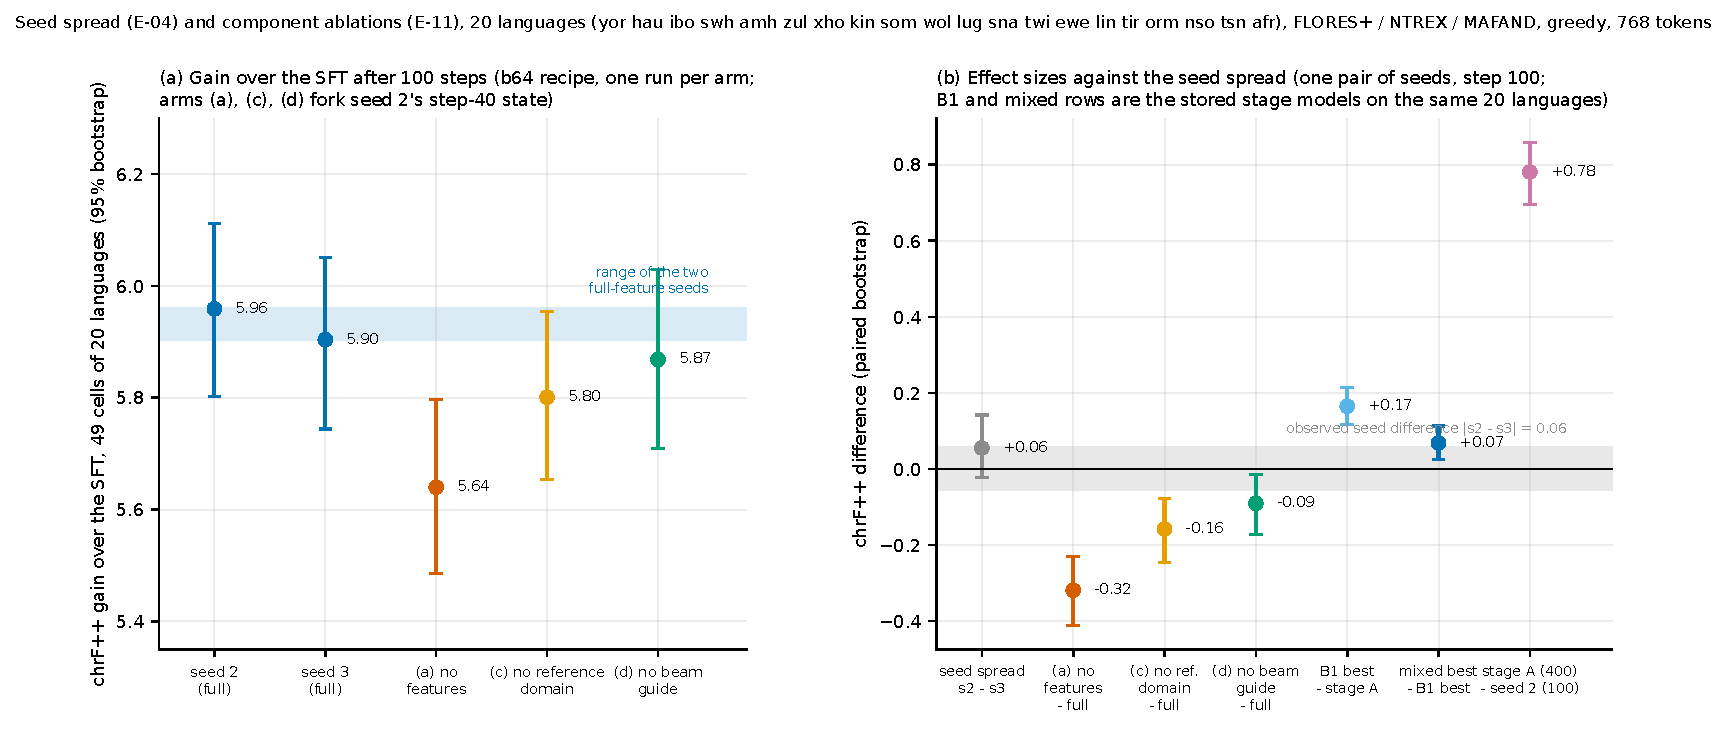
\includegraphics[width=\textwidth]{figures/fig16_e04_e11_seeds_ablations.pdf}
\caption{Seed spread (E-04) and ablation arms (E-11), 20 languages, 49 cells, greedy, 768 tokens, 95\% paired bootstrap. (a) \chrfpp{} gain over the SFT after 100 steps for two full-feature seeds and three ablation arms (shaded: range of the two seeds). (b) Effect sizes against the observed seed difference $|s_2-s_3|=0.06$: ablation arms minus seed 2, the B1 and mixed steps on the same languages, and the 400-step stage A minus seed 2. One pair of seeds, step 100.}\label{fig:seeds}
\end{figure*}

\subsection{Beam search and MBR (E-02)}\label{sec:decoding}
% [D1-D7 E02]
On 4,000 sentences (20 languages $\times$ 200 FLORES+ sentences) at 768 tokens, vLLM's beam search lets a runaway continuation beat every ended hypothesis, so the primary beam-4 (amended before any score) stops when 4 hypotheses have ended; a Hugging Face-style rule (\texttt{early\_stopping=False}) is a second beam. MBR-16 uses 16 samples plus the greedy output with \chrfpp{} as utility (metric-matched). Decoders help the SFT (beam-4 $+3.71$ \ci{+2.78}{+4.47}, MBR-16 $+5.96$ \ci{+5.37}{+6.49} \chrfpp{}); for the RL model MBR-16 adds $+0.92$ \ci{+0.81}{+1.03}, beam-4 (stop at 4) $-0.77$ \ci{-1.45}{-0.25} and the HF-rule beam $+0.83$ \ci{+0.67}{+1.00}: the sign of the RL beam result depends on the stopping rule. \textbf{Decoding does not replace RL}: RL greedy is $+1.60$ \ci{+1.34}{+1.88} \chrfpp{} ahead of the best decoded SFT (MBR-16, about 17 times the compute). RL minus SFT shrinks from $+7.56$ (greedy) to $+3.07$ (beam-4) and $+2.52$ (MBR-16): the RL gain is partly the same repair. Caveats: 20 languages, one checkpoint each; the beam numbers of an earlier 256-token study are not comparable (Appendix~\ref{app:decoding}). \textbf{Precision (E-09b):} bf16 and fp32 outputs differ between engines, but the SFT in fp32 on the full set scores $-0.04$ \ci{-0.13}{+0.07} \chrfpp{} against bf16 over the 93 cells, and the RL gain on FLORES+ is $+8.97$ \ci{+8.71}{+9.20} over the fp32 SFT against $+8.81$ over the bf16 SFT, so the bf16 harness does not overstate it; the RL model was not run in fp32.

\begin{table*}[t]
\centering\small\setlength{\tabcolsep}{3pt}
\caption{\chrfpp{} at 768 new tokens, language macro over 20 languages, 4,000 sentences per row, 95\% paired bootstrap (E-02).}\label{tab:e02}
\begin{tabular}{@{}lll@{}}
\toprule
decoding & SFT & RL (mixed best)\\
\midrule
greedy & 32.31 \ci{31.43}{33.38} & 39.87 \ci{39.17}{40.62}\\
beam-4, stop at 4 ended & 36.02 \ci{35.13}{36.95} & 39.10 \ci{38.20}{39.96}\\
beam-4, HF rule & 33.26 \ci{32.22}{34.46} & 40.70 \ci{40.00}{41.42}\\
MBR-16 & 38.27 \ci{37.60}{39.01} & 40.79 \ci{40.09}{41.54}\\
\bottomrule
\end{tabular}
\end{table*}

\subsection{Matched-compute continued-SFT control (E-03)}\label{sec:control}
% [R14 CTL7-CTL11] reports/e03_sft_control_2026-11-05.md; GATE E-03
To ask whether the GPU time of the RL chain (8.66 \GPUh{}) would do as well as more SFT, we continued the SFT final for 6,000 steps (8.4 h) at a constant learning rate of $10^{-5}$ (chosen by a probe fixed in advance), with 16 replay packs and 16 packs of TranslatePsy English-to-X pairs \citep{gritta2026translatepsy} per step: NLLB-3.3B translations of MADLAD-400 sentences for 19 languages, 277,900 pairs each, scanned against the protected index and used once. The decision rule, primary endpoint (language-macro \chrfpp{} over 93 cells, RL minus control) and language panels were written down before any benchmark of the control was looked at. \textbf{Only the 6,000-step checkpoint was evaluated}; the stage-A-matched (3,100) and mixed-best-matched (4,800) checkpoints exist but were not evaluated.

\begin{table}[t]
\centering\footnotesize\setlength{\tabcolsep}{3pt}
\caption{Continued-SFT control against the RL mixed best; language-macro \chrfpp{}, clean rows, 95\% paired bootstrap; TP = the 19 TranslatePsy languages. Held-out AfriCOMET, RL $-$ control: $+0.0183$ (all), $-0.0249$ (TP), $+0.0883$ (other).}\label{tab:e03}
\begin{tabular}{@{}lccl@{}}
\toprule
cells & control & RL & RL $-$ control\\
\midrule
all (93) & 29.97 & 34.55 & $+4.58$ \ci{+4.45}{+4.70}\\
TP (47) & 41.37 & 41.34 & $-0.03$ \ci{-0.13}{+0.09}\\
other (46) & 18.32 & 27.61 & $+9.29$ \ci{+9.09}{+9.49}\\
\bottomrule
\end{tabular}
\end{table}

The registered rule had four conditions: lower bound of the overall difference above $+1.0$ (met: $+4.58$ \ci{+4.45}{+4.70}), AfriCOMET lower bound above 0 (met: $+0.0183$ \ci{+0.0172}{+0.0192}), difference above 0 on the other languages (met) and difference above 0 on the 19 TranslatePsy languages (\textbf{not met}: $-0.03$). \textbf{By the rule as registered the verdict is ``inconclusive''}, and we did not change the rule. Reading the panels: where a teacher-translated corpus exists, continued SFT matches RL in \chrfpp{}, largely fixes finishing and looping (FLORES+ finished 0.993 against 1.000 for RL), and is ahead on the neural metrics; on the other languages it changes almost nothing ($+0.15$ \chrfpp{} over the SFT on FLORES+, \ci{-0.03}{+0.32}), while RL improves them all from its own samples ($+9.29$). The overall endpoint alone reads ``RL is better'', the 19 languages alone ``comparable''; neither is the registered verdict. Caveats: one seed, one learning rate, one budget point; the control is not information-matched (NLLB-3.3B scores 38.80 against 26.30 for the SFT on 43 languages), and the TranslatePsy rows were filtered with AfriCOMET, SSA-COMET and MetricX, so those neural metrics favour the control; chrF and \chrfpp{} are the evidence.

\begin{figure*}[t]
\centering
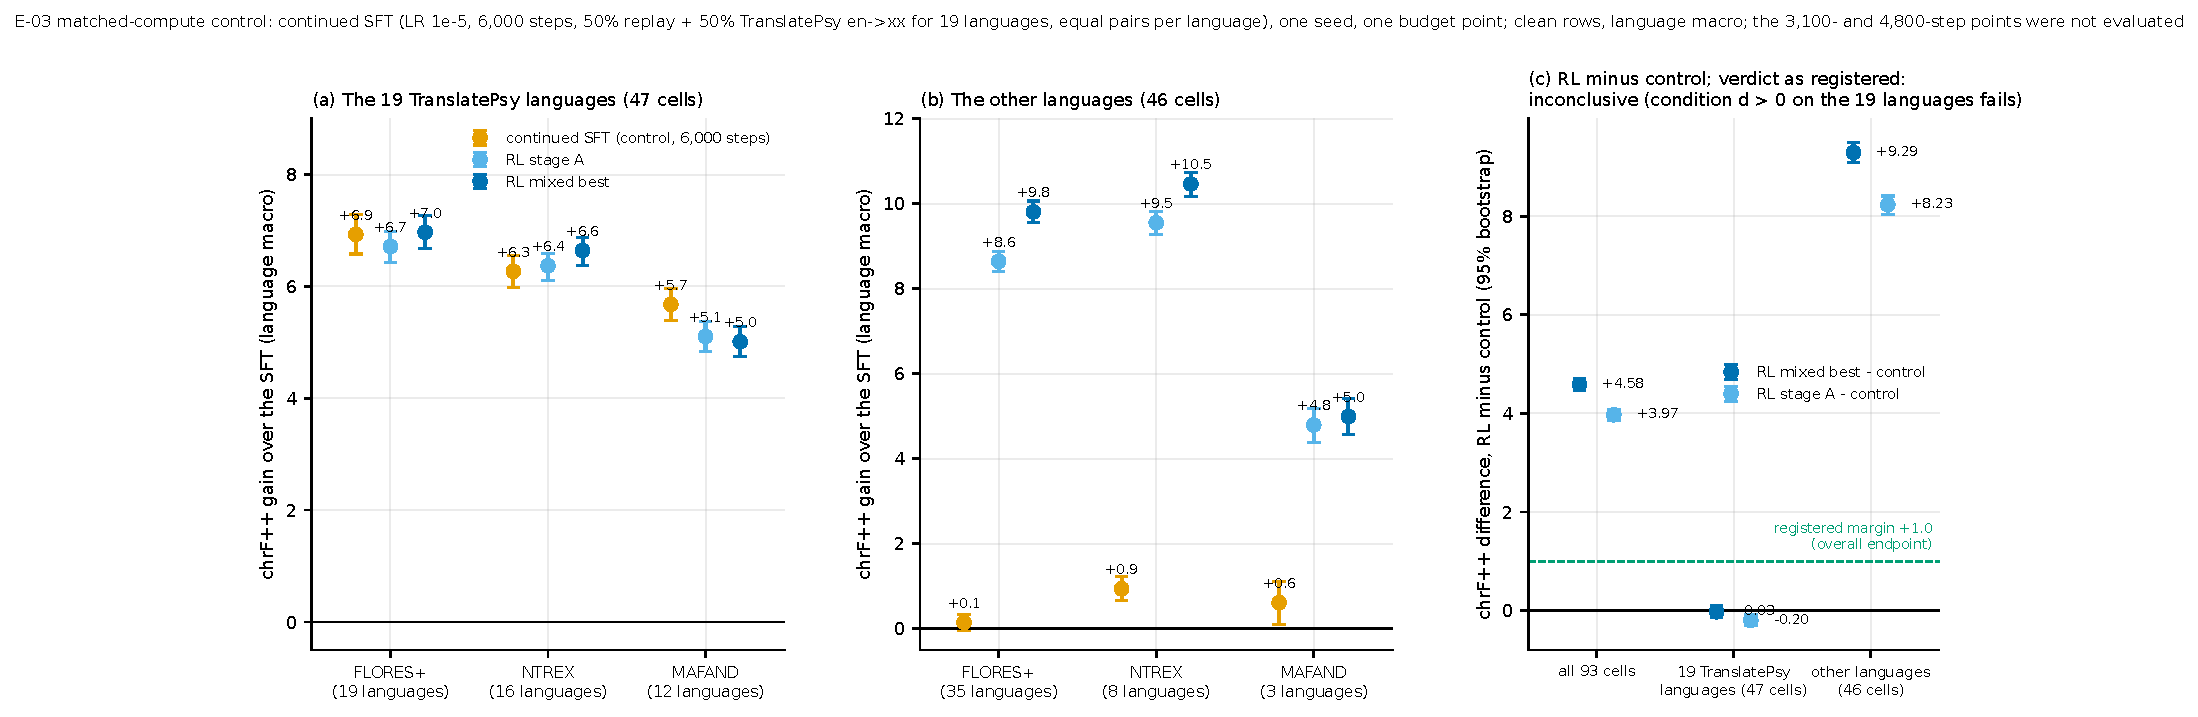
\includegraphics[width=\textwidth]{figures/fig14_e03_control.pdf}
\caption{Matched-compute continued-SFT control (E-03). (a, b) \chrfpp{} gain over the SFT (language macro, 95\% bootstrap) of the control, RL stage A and RL mixed best by benchmark, for the 47 cells of the 19 TranslatePsy languages (a) and the 46 other cells (b). (c) RL minus control for all 93 cells and for the two panels, with the registered $+1.0$ margin; the registered verdict is inconclusive. One seed per model; only the 6,000-step checkpoint was evaluated.}\label{fig:e03}
\end{figure*}

\subsection{Comparison with NLLB-200}\label{sec:nllb}
% [N1-N6 NLLBRL]
NLLB-200 3.3B (the 3.3B variant of its model card) has about 8.6 times the parameters of our 385M model. On the 43 languages shared with the published FLORES-200 devtest table, the mixed best reaches 35.54 \chrfpp{} against 38.80 for NLLB-3.3B ($-3.26$, language-bootstrap \ci{-4.29}{-2.20}; 92\%; SFT 26.30, $-12.50$, 68\%): RL closes 74\% of the gap, and the remaining gap is not a finishing artefact (the mixed best finishes at least 0.99 in every language). It matches or beats NLLB-3.3B on 7 of 43 languages, all in the lowest tertile (e.g. yor $+5.43$, fon $+2.95$); the largest gaps are amh $-11.28$, kin $-9.74$, kea $-8.72$. Caveats: FLORES-200 against FLORES+ references, NLLB beam against our greedy (beam and MBR move our \chrfpp{} by $-0.77$ to $+0.92$), the 11 hardest languages have no NLLB row, five of the 43 languages had an NLLB pseudo-reference reward term, the yor value is anomalously low, intervals are over languages, one seed. We state only that, size-aware, the model reaches 92\% of NLLB-3.3B's \chrfpp{} on these languages and matches or beats it on 7 of 43; we do not claim to beat NLLB or to be competitive with it overall.

\begin{figure*}[t]
\centering
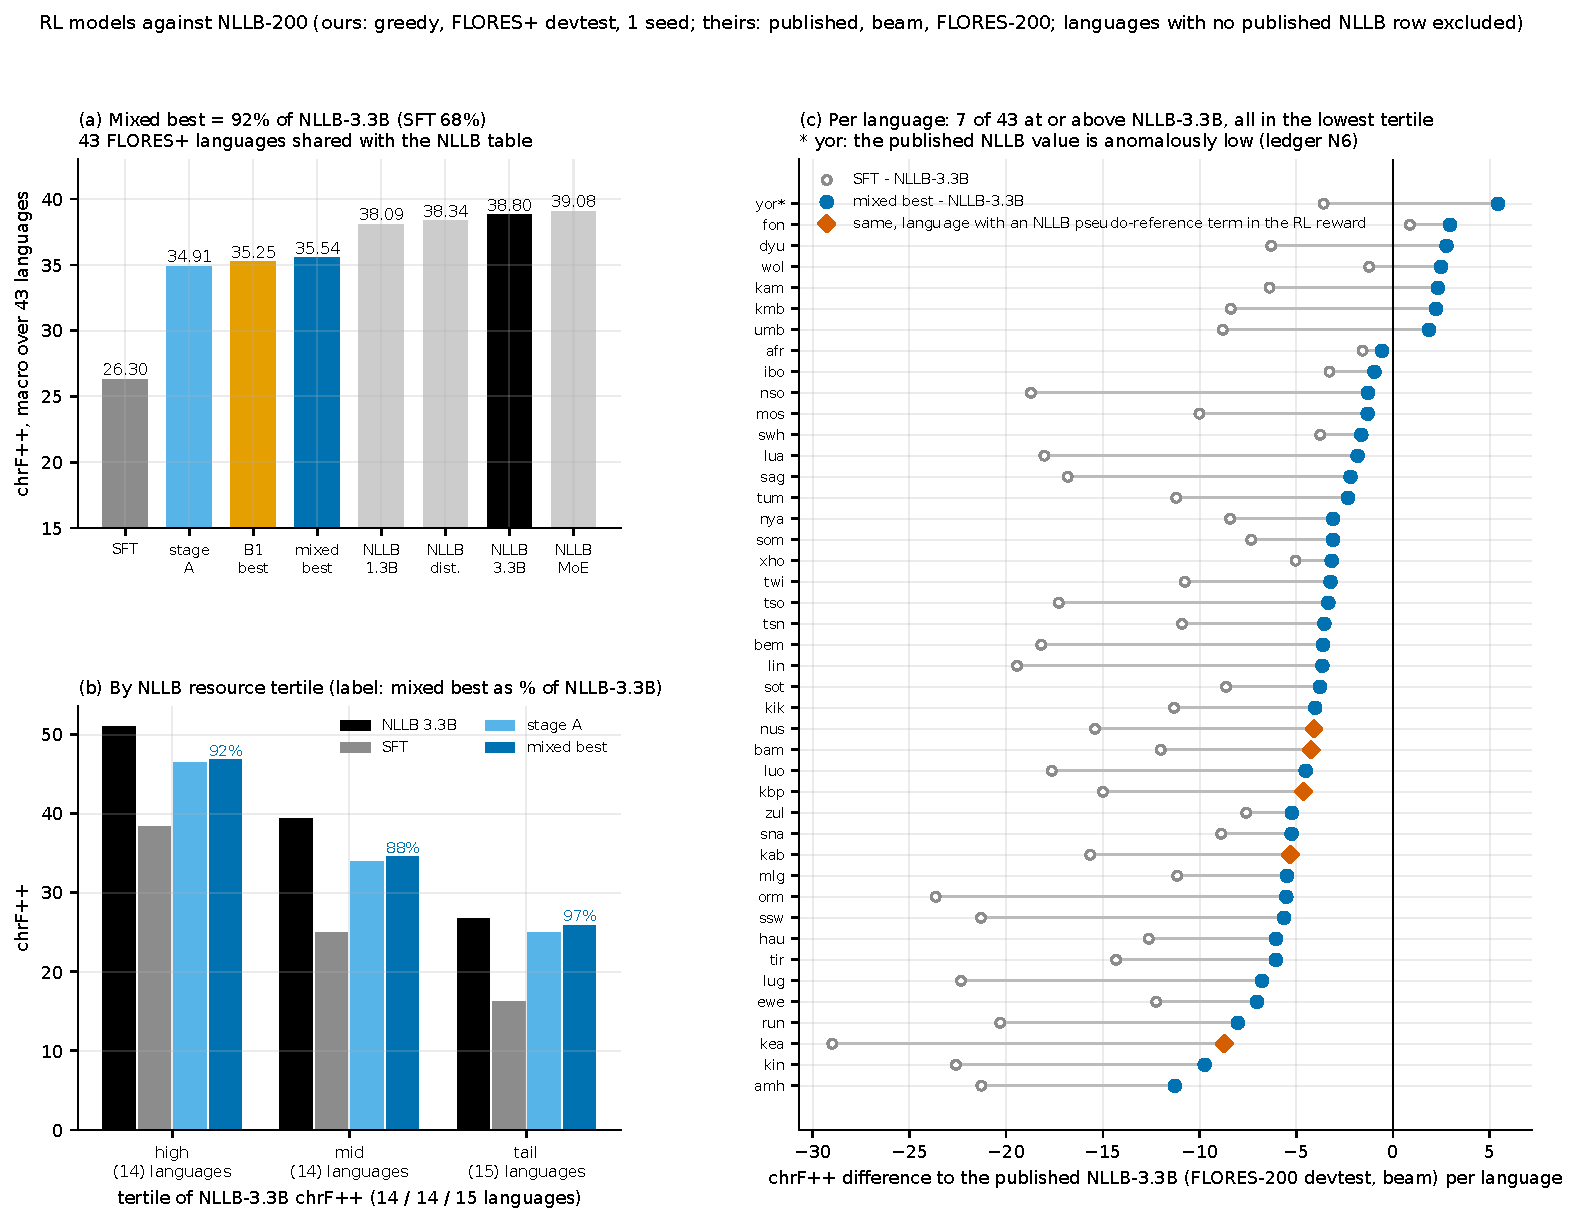
\includegraphics[width=0.62\textwidth]{figures/fig4_nllb_43.pdf}
\caption{RL models against NLLB-200 on the 43 shared FLORES+ languages (ours: greedy, one seed per model; NLLB: published FLORES-200 devtest, beam). (a) Language-macro \chrfpp{}: mixed best 35.54 against NLLB-3.3B 38.80 (92\%; SFT 68\%). (b) By tertile of NLLB-3.3B \chrfpp{} (14/14/15 languages). (c) Per-language difference to NLLB-3.3B, SFT (open) and mixed best (filled); orange diamonds: languages with an NLLB-3.3B pseudo-reference reward term; yor$^*$: anomalously low published value. Intervals are over languages only.}\label{fig:nllb}
\end{figure*}

\subsection{Science and long-document RL}\label{sec:science}
% [SC1-SC6 DL1-DL5 P4 E05 E15 E16]
A science SFT with weight interpolation ($\alpha=0.5$) gives surface gains on AfriScience-MT (chrF $+1.2$) and no SSA-COMET-QE gain (0.6130 to 0.6118). A science RL adds $+0.46$ chrF \ci{+0.27}{+0.65} and $+0.0053$ AfriCOMET on test sentences over its start, and nothing at document level. \textbf{The science SFT, not the science RL, carries the science gain (E-14):} the same RL started from the mixed best, without the science SFT, ends $-1.44$ chrF \ci{-1.61}{-1.25} and $-0.0082$ AfriCOMET \ci{-0.0101}{-0.0065} below the executed science RL and adds only $+0.26$ chrF \ci{+0.12}{+0.39} over its start, so by the registered rule the science SFT is needed; SSA-COMET-QE rates it level ($-0.0006$ \ci{-0.0018}{+0.0007}), a reward-family effect rather than evidence of quality. One seed, one out-of-memory restart, final checkpoint only (Appendix~\ref{app:docs}). Whole-document generation (4,096 tokens) fails for the 385M models; a long-document RL raises whole-document finishing from 0.70 to 0.82 ($+0.125$ \ci{+0.046}{+0.204}) and lowers the loop rate from 0.85 to 0.73, but 72 to 73\% of documents still loop and chunked decoding is required; the earlier 270M model is as good or better at document level. Table~\ref{tab:sci} gives sentence-level scores for every stage (SSA-COMET-QE is of the reward family; the first RL stage adds $+0.043$ and later stages at most $+0.005$ more, while chrF and AfriCOMET keep rising slightly).

\begin{table}[t]
\centering\footnotesize\setlength{\tabcolsep}{3pt}
\caption{AfriScience-MT test, sentence level (970 sentences per language; macro over amh hau lug nso yor zul; greedy; one seed per stage). SSA-QE = SSA-COMET-QE, of the reward family for every RL row.}\label{tab:sci}
\begin{tabular}{@{}lccc@{}}
\toprule
stage & chrF & AfriCOMET & SSA-QE\\
\midrule
SFT & 36.00 & 0.6064 & 0.5686\\
RL stage A & 45.06 & 0.6822 & 0.6118\\
RL mixed best & 45.40 & 0.6828 & 0.6130\\
science RL w/o SFT (E-14) & 45.66 & 0.6850 & 0.6153\\
science SFT ($\alpha=0.5$) & 46.63 & 0.6879 & 0.6118\\
science RL final & 47.10 & 0.6932 & 0.6158\\
long-document RL final & 47.16 & 0.6936 & 0.6165\\
\bottomrule
\end{tabular}
\end{table}

\section{Discussion and Conclusion}\label{sec:discussion}
% [paper.md 12.1-12.3; GATE E-01 E-03]
Under automatic metrics, RL with reference-free QE rewards beats the SFT everywhere, but about half of the \chrfpp{} gain (49\%; 29\% of the AfriCOMET gain) is finishing and looping that a one-line decode-time guard also removes, and beam/MBR decoding repairs a further part. What RL adds beyond a guarded SFT is $+4.37$ \chrfpp{}; nearly all of it arrives in the first stage, and the mixed step is not separable from seed noise. Our reading, only partly tested, is that the SFT's main defect is unguarded greedy decoding and that the hard-failure floor and the QE reward teach the policy to avoid it within about a hundred steps. Against continued SFT for the same GPU time the registered verdict is ``inconclusive'': the control matches RL on the 19 languages it has teacher data for and does nothing for the other 46 cells, so what RL contributes, in our data, is breadth. We do not claim that the \chrfpp{} beyond finishing is quality a human would confirm, that any reward component other than the stage-A features helped, or that the model is usable for Arabic dialects, Tamazight, Dinka, Tamasheq or Kanuri. In science translation the science SFT, not the science RL, carries the gain (E-14: the same RL without it ends $-1.44$ chrF \ci{-1.61}{-1.25} lower). Next experiments: stronger guards in full evaluation, the unevaluated control checkpoints, later-stage seeds and human judgement of outputs.

\FloatBarrier\label{coreend}
\clearpage
\section*{Limitations}
% [paper.md section 13; full list in the appendix of the full version]
\textbf{Automatic scoring only.} The references of FLORES+, NTREX-128 and MAFAND-MT are human translations, but all scoring is automatic: no human judgement of system outputs was collected. The neural scores belong to one family, and AfriCOMET has a length and entity bias.
\textbf{One training run per model.} We measured seed noise only for the first RL stage, on 20 languages and 100 steps, with one pair of extra seeds. The last RL step and per-language differences below about half a point cannot be separated from seed noise. A second seed of the SFT baseline is impractical (about 45 GPU-hours).
\textbf{The matched-compute control is one run:} one seed, one learning rate, one data mix with NLLB-3.3B targets and one evaluated stopping point. The repetition-penalty control chose its best value at the edge of the range searched.
\textbf{Rewarded metrics are not evidence.} The finished, repetition and language checks, and the quality scores the RL optimises, are part of the reward. The independent repetition detector shares the idea of the reward's check and cannot see non-repetitive failures.
\textbf{Ablations are limited:} three arms, 100 steps, one run each, 20 languages; later RL stages and most reward ingredients were not ablated, and mid-run changes (Ethical considerations) mean the stages are not one clean design.
\textbf{Decoding and engine.} Headline numbers use one inference engine in bf16. The two engines differ in bf16 but agree in fp32; we did not run the RL model in fp32. Beam search and MBR cover 20 languages and one beam width.
\textbf{Coverage and comparisons.} Fifty-one of the 125 languages have no reference test and are unscored. The model fails on Arabic dialects, Tamazight, Dinka, Tamasheq and Kanuri, where RL increases English output. Comparisons with the earlier 270M model and with NLLB mix differences in data, steps, test sets and decoding: our decoding is greedy, NLLB's is beam search, and on NTREX and MAFAND-MT only language-level NLLB averages exist (no sentence pairing, no AfriCOMET). Document results rest on 28 papers per language, and whole-document translation remains unusable.
\textbf{Not run.} Human judgement of outputs; the NLLB-data ablation; scans of packed training shards for contamination; a 54-language decoding study; a science fine-tuning step at full strength followed by RL; a second seed of the science run; long-document RL from the no-science-step model.

\section*{Ethical considerations}
% [DISCLOSURES sections 1-6; L1-L5 CT1-CT13 CTL1-CTL6; CFU]
\textbf{Data and licences.} NLLB-mined bitext (OPUS-NLLB, 43 languages; Fulah) is 14.4\% of the 3.990\,B stage-B pack tokens (10.84\% of the 5.043\,B tokens drawn in the whole SFT); with NLLB-Seed and the aligned part of Aya (NLLB-3.3B outputs) 18.7\%; with machine-translated Tumbuka instruction sets (system not stated, possibly NLLB) 22.8\%. NLLB models and outputs carry CC-BY-NC terms, which limits the commercial use of NLLB-derived data and signals, and a licence statement must accompany any release of the weights. Sources with unspecified or unconfirmed licences (the \texttt{*\_mt560} OPUS sets, 69\% of the main pair output, mostly Jehovah's Witnesses and Bible text; \texttt{multi-open}; AfroLingu-MT; an Efik New Testament sheet) need a legal decision, and religious text dominates many low-resource languages. IbomMT (CC-BY-NC-4.0) is a disclosed non-commercial exception. NLLB-3.3B pseudo-references (CC-BY-NC) are a reward signal for five languages, reward only. RL prompts (FineWeb-Edu, Wikipedia, news including BBC News with no declared licence and BBC copyright) are input text only. Gemma terms apply to the derived weights and its pretraining exposure cannot be excluded. Reward and monitor models, as declared on the Hub (read 2026-11-05): \texttt{ssa-comet-mtl}, \texttt{ssa-comet-qe} and the two AfriCOMET checkpoints apache-2.0; GlotLID \texttt{license: other} with \texttt{license\_name: apache-2.0-plus-notices} (Apache License 2.0 plus notices).

\textbf{Release and licence.} \anonreal{Checkpoints are anonymised for review and released on acceptance; the control checkpoint of E-03 is not released.}{The final RL model (branch \texttt{main}, the mixed best) is at \url{https://huggingface.co/AletheiaAING/gemma-0.4B-translate-rl}, the SFT model at \url{https://huggingface.co/AletheiaAING/gemma-0.4B-translate-sft} and the seed, ablation and E-14 weights at \url{https://huggingface.co/AletheiaAING/gemma-0.4B-translate-rl-experiments}; the control checkpoint of E-03 is not released.} At the last check the Hub repositories declare no licence field and have no model card; the Gemma terms of use apply to the derived weights, and the NLLB-derived and non-commercial data above limit commercial use \ownerdecision{confirm release licence}. The state, prompts, eval and reports repositories were private at the last check \ownerdecision{which parts of the data are released}.

\textbf{TranslatePsy.} \texttt{qvac/\allowbreak TranslatePsy-\allowbreak AfriSLM-\allowbreak Synthetic-\allowbreak Mix} (CC-BY-NC-4.0; targets are NLLB-3.3B translations of MADLAD-400 sentences filtered by AfriCOMET, SSA-COMET and MetricX) was used for the matched-compute control only. No TranslatePsy row is in the SFT, any RL stage, the science or long-document stages or any released weight; the control checkpoint is a research artefact that is neither released nor used in production. A good control result partly means ``distilling NLLB''. The NLLB-218 language-ID model (CC-BY-NC) was used for measurement only.

\textbf{Decontamination residuals (this pipeline, the clean 385M rerun).} The audit of the 385M training text finds no benchmark sentence of three or more words; benchmark rows that match are one- or two-word strings, numerals and names (NTREX 120 of 47,928 rows, 0.25\%; MAFAND-MT 94 of 20,009, 0.47\%; SmolSent 45 of 38,833; GlotStoryBook 15 of 3,426). The FLORES+ dev train half (440 ids) is in training on purpose and the held-out half is protected. A lexical fuzzy scan (56,975,939 pair rows, 4,277,612 instruction rows) finds no benchmark string of 8 or more tokens as a contiguous run, but strings of 4 to 7 tokens occur inside longer text (English side: MAFAND-MT 134 of 17,428, GlotStoryBook 30 of 898, NTREX 18 of 1,973, SALT 12 of 498) and 263 (string, benchmark) cases of 8+ token strings overlap training text by character 5-grams (candidates, effect on scores not measured). Stage A drew 6 flagged prompts of 28,120 (0.021\%) from seven unfiltered prompt files; 305 of 34,007 AfriScience-MT train rows (0.9\%) have their African-language sentence in the A0 pair data (test papers untouched). Embedding or MT-round-trip paraphrase scans and packed-shard scans were not run. Statements about the earlier 270M pipeline, whose training text held the English side of 95\% of FLORES+ devtest, do not apply to this rerun; its numbers appear only on rows clean for both generations.

\textbf{Analysis decisions and process.} Checkpoints were selected on a 720-sentence FLORES+ dev subset; the weak-language choice used devtest-derived per-language tables; the decomposition and family analyses were run after the results were known; the science headline metric changed after the interpolation rule was written. The RL preflight and stage-A gates failed and were overridden by the authors; stage A was stopped at step 40 and resumed with four features; B1 was restarted twice and the mixed stage once (the hacking alarm was loosened); the science-RL step cap was extended from 150 to 190 and the run stopped on a dev plateau after 160 steps; the long-document RL lost about 4.5 of 7.7 h to a crash loop, and the E-14 run had one out-of-memory restart (steps 21 to 38 replayed; the later records are used). LibreTexts rows were removed from the long-document pool before it started.

\textbf{Intended use, risks and dual use.} Outputs are machine translations of unverified quality for languages without human judgement, with documented failure modes (Arabic dialects, Tamazight, Dinka, Tamasheq and Kanuri are not usable; RL increases English output there; use sentence by sentence, not on whole documents). The model should not replace NLLB-class systems or be used where mistranslation is costly (health, legal, safety). As with any translation model it can be used to produce text at scale in under-served languages, including spam or misleading content, and we release no content-filtering component. Released artefacts are anonymised for review and released on acceptance.

\ifanon\else
\section*{Author contributions}
\textit{[Placeholder, to be filled by the lead author: one sentence per person describing what that person contributed (for example design, data, training, evaluation, writing). Authorship is based on contribution.]}
\fi
\bibliography{refs}
\bibliographystyle{acl_natbib}

\clearpage
\appendix
\label{appstart}
\onecolumn
% Appendix: generated from paper_385m/paper.md by a small converter, then kept as hand-editable LaTeX. Report keys and claim IDs are in % comments.

\FloatBarrier

\section{Hyper-parameters, recipe and reward details}\label{app:hyper}

This appendix collects the SFT and RL settings that Sections~\ref{sec:method} and~\ref{sec:method} summarise.

\subsection{SFT recipe and learning-rate schedule}

\textbf{Recipe.} Samples are packed into 4,096-token packs (one language per pack, block-diagonal attention) at 32 packs = 131,072 tokens per step; each pack is used once. Optimiser: Muon (momentum 0.95, 5 Newton-Schulz steps) on the 2-D decoder matrices and AdamW (betas 0.9/0.95) on embeddings and norms, weight decay 0.01, gradient clipping 1.0, 3\% linear warm-up then cosine decay, seed 1234. The learning-rate schedule, read from the executed per-shard configs, is: SFT-1 (\texttt{g1a}, 1,500 steps) peak 5e-5, cosine to 50\% of the peak (2.5e-5); shard 1 (\texttt{g1b\_\allowbreak{}s1}) peak 5e-5, cosine to 80\% (4e-5); shards 2-5 (\texttt{g1b\_\allowbreak{}s2}..\texttt{g1b\_\allowbreak{}s5}) peak 3e-5 (lowered from 5e-5 on 2026-11-01 because of forgetting in tiny languages), cosine to 80\% (2.4e-5); shard 6 (\texttt{g1b\_\allowbreak{}s6}) peak 3e-5, cosine to 10\%, so the last step runs at 3.0e-6. Every shard starts a fresh Muon state with a 3\% linear warm-up. SFT-2 runs in six shards of about 4,800 to 5,300 steps, with tail-language replay from shard 2. Executed stage B: 31,353 steps, 4.109 B tokens, 5.14 s per step on an A100 (44.8 h); 32,853 steps in all with SFT-1. Final validation loss: macro 1.3412, micro 1.2846 over 78 languages (end of SFT-1: 1.7847). The macro rises from 1.78 to 1.98 at the end of shard 1 because new languages enter the validation set at stage 2.  
% src: VERIFIED against the executed per-shard configs (`learning_rate`, `min_lr_ratio`, `warmup_ratio`, `init_from` keys): `reports/data/e23_hygiene_2026-11-04/sft_configs/g1a.yaml`, `g1b_s1.yaml` ... `g1b_s6.yaml` (copies of the box files `clean_sft_small/run/configs/growth1/`). The repository templates `gemma_mt/configs/growth1/g1a.yaml` (5e-5, min_lr_ratio 0.5) and `g1b.yaml` (5e-5, min_lr_ratio 0.1) are NOT the executed shard configs: `g1b.yaml` is the single-shard template (peak 5e-5, floor 10%); `gemma_mt/configs/clean_rerun_sft/` holds the A0 configs only. Resolves the HYG M4 vs CTLP disagreement: HYG's "cosine to 10%" is right only for shard 6 (and the g1b template); CTLP's 0.8 for shards 2-5 is right; shard 1 also 0.8 and SFT-1 0.5, neither stated in HYG or CTLP. Other keys common to all: Muon momentum 0.95, 5 NS steps, weight decay 0.01. Validation: HYG M4 (sft_385m_curve.csv, sft_385m_val_by_language_final.csv); NLLBLINK for 44.8 h

\begin{figure}[t]
\centering
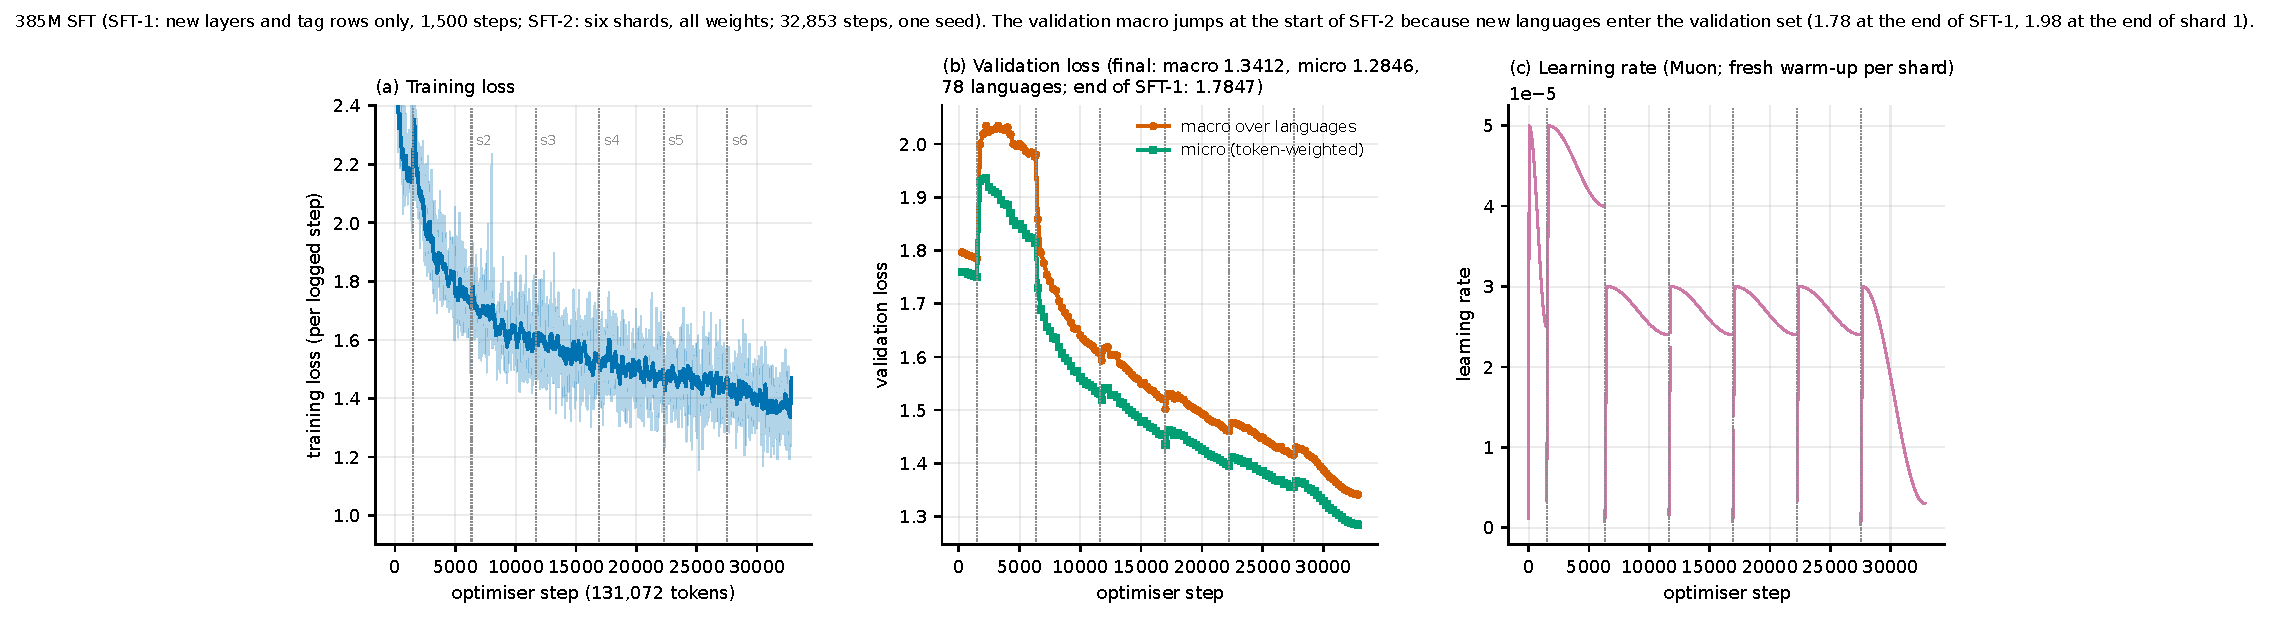
\includegraphics[width=1.00\linewidth]{figures/fig13_sft_validation_curve.pdf}
\caption{Training of the 385M SFT (one seed): (a) training loss per logged step (thin) and 20-point mean (thick), (b) validation loss (macro over languages and token-weighted micro) and (c) learning rate over the 32,853 optimiser steps of SFT-1 (1,500 steps, new layers and tag rows only) and the six SFT-2 shards (dotted lines); the validation macro jumps at the start of SFT-2 because new languages enter the validation set, and the learning-rate panel shows the per-shard schedule of Section~\ref{sec:method}. Final validation loss: macro 1.3412, micro 1.2846 over 78 languages. Source: \texttt{reports/\allowbreak{}data/\allowbreak{}e23\_\allowbreak{}hygiene\_\allowbreak{}2026-\allowbreak{}11-\allowbreak{}04/\allowbreak{}sft\_\allowbreak{}385m\_\allowbreak{}curve.\allowbreak{}csv}.}\label{fig:fig13_sft_validation_curve}
\end{figure}

\subsection{RL: optimiser, stages, prompts, reward and features}

\textbf{GRPO as used.} One on-policy update per sampled batch; a prompt gets a group of 16 completions (15 sampled plus the greedy output; in guided groups 14 sampled, the guide and the greedy output); the advantage is the group-standardised reward; the loss is the token-level policy-gradient term plus a k3 KL penalty to a reference model (coefficient 0.05 in stages A to mixed; the reference is the start model of each stage, i.e. the SFT final for stage A and the previous stage's checkpoint afterwards, because every stage restarts with a fresh reference and a fresh optimiser) \citep{shao2024deepseekmath,schulman2020approximating}. Optimiser: Muon (momentum 0.95, 5 Newton-Schulz steps), \textbf{learning rate 2e-6} with 10 warm-up steps, weight decay 0, gradient clipping 1.0; temperature 1.0, top-p 1.0; at most 384 new tokens in the short-window bin (b64) and 1,280 in b256 and the mixed stage; seed 1234. A KL guard cuts the learning rate when the median KL exceeds a threshold (0.15 in stage A, 0.25 later). Prompts per step: 64 in stage A, 48 in B1, 42 in mixed. 
% src: HYG section 3 (M7: runs_385m/{A,B1,mixed}/config.json, copies in reports/data/e23_hygiene_2026-11-04/rl_configs/); repository configs gemma_mt/configs/clean_rerun_385m/rl_A_b64.yaml, rl_B1_b256.yaml, rl_C_mixed.yaml (learning_rate 2.0e-06, kl_coef 0.05, model_name = KL reference AND policy start); reports/rl_stage_A_385m_2026-11-03.md; reports/rl_vs_sft_evidence_2026-11-04.md section 6

\begin{table}[t]
\centering\scriptsize
\setlength{\tabcolsep}{4pt}
\caption{RL hyper-parameters by stage.}\label{tab:stagecfg_full}
\begin{tabularx}{\linewidth}{@{}lrrr>{\raggedright\arraybackslash}X>{\raggedright\arraybackslash}X@{}}
\toprule
stage & learning rate & KL coefficient (k3) & group size & guide member & steps (cap) $\times$ prompts \\
\midrule
A, B1, mixed & 2e-6 (10 warm-up steps) & 0.05 & 16 (15 + greedy) & beam/MBR, fraction 0.25 (from step 41 in A) & 400 $\times$ 64; 150 (135 run) $\times$ 48; 60 $\times$ 42 \\
science RL & 1.0e-6 & 0.1 & 16 & beam/MBR, fraction 0.25 & 150 in the yaml, cap extended to 190 by the extension rule at step 120; executed 160 (stopped at step 150 by dev plateau, then 10 wind-down steps; \texttt{summary.\allowbreak{}json}, Appendix~\ref{app:chain}) $\times$ 42 \\
long-document RL & 1.0e-6 & 0.1 & 8 (7 + greedy) & off & 80 $\times$ 32 (51\% long prompts) \\
\bottomrule
\end{tabularx}
\end{table}

The science SFT before the science RL used AdamW at 3e-6 (Section~\ref{sec:science}). Dynamic-sampling, std-floor and reference-domain settings differ by stage as well (Appendix~\ref{app:chain}). 
% src: A to mixed: gemma_mt/configs/clean_rerun_385m/rl_{A_b64,B1_b256,C_mixed}.yaml. Long-document RL: gemma_mt/configs/clean_rerun_385m_long/rl_F_final.yaml (learning_rate 1.0e-06 "D-59", kl_coef 0.1, group_size 8, guide_fraction 0.0, steps 80, prompts_per_step 32, extend_if_improving false, KL reference = the start model). Science RL: `clean_rerun_385m_sci/rl_F_final.yaml` on the A100 box (the file that runs): Muon, LR 1.0e-6, KL coefficient 0.1 with the start model as reference (D-59), group 16, guide fraction 0.25, as read by the coordinator on 2026-11-04; The file is stored at reports/data/rl_configs_as_executed_2026-11-04/sci_rl_F_final.yaml (reproducibility list of the draft). Closes the LDOC "KL coef 0.1 / 1e-6" flag; the `kl_coef` comment of the long-document yaml adds that the old final run's yaml said 0.05 but its CLI override executed 0.1

\textbf{Stages.} Stage A (400 steps, short English windows, bin b64), B1 (135 steps run, b256; best checkpoint step 50 by dev chrF++), mixed (60 steps, b64 and b256), then a continued-RL run on eight weak languages (85 steps), a science SFT with weight interpolation, a science RL and a long-document RL (Appendix~\ref{app:chain}). B1 started from stage A's final model (step 400), mixed from B1's best checkpoint (step 50), the weak-group run from the mixed best, the science SFT from the mixed best. The dev set has \textbf{720 sentences = 18 FLORES+ dev languages $\times$ 40 sentences} (afr ewe fon hau ibo kin nya orm sna som sot swh tsn twi wol xho yor zul). B1's step-135 weights (\anonreal{an anonymised checkpoint}{Hub branch \texttt{stage-\allowbreak{}b1-\allowbreak{}final}}) were evaluated after the fact (E-20, Section~\ref{sec:seeds}) and equal B1 best within noise. 
% src: HYG X3, X4, X19; ledger M8. Step 200 of stage A was the dev-best checkpoint at its time (dev 40.4697); the final model of step 400 (dev 40.50, a gain of 0.03 below the selection minimum 0.1) is the one every evaluation uses

\textbf{Prompts.} English windows of consecutive sentences from FineWeb-Edu and Wikipedia (70\%) and from news (BBC, Wikinews, Global Voices, and Wikivoyage; 30\%), filtered against the protected index; 81 languages with higher draw weights for the 29 weakest. The stage-A news pool contained Wikivoyage (\texttt{darkpredator/\allowbreak{}stealth-\allowbreak{}wikivoyage-\allowbreak{}en}; 188 prompts drawn in steps 1-400) and an unlisted source \texttt{SetFit/\allowbreak{}bbc-\allowbreak{}news} (37 pool rows, none drawn). 
% src: reports/rl_prompts_news_2026-11-03.md; reports/rl_stage_A_385m_2026-11-03.md; ledger L5, CT13; CFU section 1

\textbf{Reward.} Per completion: hard failures (missing or wrong language tag, unfinished or text after the end token, copy of the source, degenerate repetition, wrong language by GlotLID \citep{kargaran2023glotlid} with a 15-character minimum, length outside the human window) receive the floor reward \ensuremath{-}2. Otherwise the content signal is a reference-free quality-estimation ensemble of \texttt{masakhane/\allowbreak{}africomet-\allowbreak{}qe-\allowbreak{}stl-\allowbreak{}1.\allowbreak{}1} \citep{wang2024africomet} (r1) and \texttt{McGill-\allowbreak{}NLP/\allowbreak{}ssa-\allowbreak{}comet-\allowbreak{}mtl} run without a reference \citep{li2025ssacomet} (r2), each shaped per language onto a monotone curve calibrated on human references (held-out calibration split of 261 ids, never dev, devtest or test). \textbf{The ensemble is the mean of the two shaped rewards if |r1 - r2| $\le$ 1.0 and the minimum otherwise}; it exists for 42 languages (41 with an ensemble block; Dyula has none). For languages without a validated QE model the content signal is the consensus (mean sentence chrF++ against the other valid group members, at least 3 valid members, blend 0.5); for five weak languages (kea kbp nus bam kab) an NLLB-3.3B pseudo-reference chrF++ term is added with weight 0.25 (max 0.35), reward only. Penalties are penalties only (never a bonus), as executed in stages A, B1 and mixed: length (weight 1.0 per log-unit outside the language's human length-ratio window, widened by 15\%), word ratio (0.5 per log-unit of the words ratio above the human 99th percentile, slack 15\%), lexical (1.0 per unit of deficit in numbers, names and content words that are not in the source), diacritics (1.0), and the constraint anchors (boilerplate, copy with cap 2.0, entity recall 0.5, function words 0.3, padding, repetition and a lexicon guard; v1 for consensus and blend languages, v2 for all three content modes; a saturated stuffing deficit at 0.9 is a hard failure); the fluency and science-anchor penalties were off; hard-failure classes also include an empty output. The reward range is [\ensuremath{-}2, 2.25]. The reward is computed per sentence chunk and aggregated by source length, with failed chunks at \ensuremath{-}2 (long-document reward \texttt{longdoc\_\allowbreak{}v2}, applied to short bins too). 
% src: HYG section 3 (M9: gemma_mt/gemma_mt/rl/qe_ensemble.py header, shaping_clean_v2.json `ens_delta` 1.0, training_state reward_range); reports/rl_vs_sft_evidence_2026-11-04.md section 1 (reward-family table); reports/rl_stage_plan_385m_b256_2026-11-02.md section 3; penalty list read from the reward code and the executed configs (`research_archive_2026-11-03/box_final_2026-11-04/clean_rerun/tree/gemma_mt/gemma_mt/rl/reward.py`; `reports/data/e23_hygiene_2026-11-04/rl_configs/config_{A,B1,mixed}.json`, identical reward block in A, B1 and mixed)

\textbf{Four features added at step 41 of stage A.} Stage A ran steps 1-40 without them; at the step-40 checkpoint the trainer was stopped and resumed from \texttt{last/\allowbreak{}} with all four switched on. (1) Dynamic sampling: oversample 1.1 (later 1.0), drop flat groups, refill up to twice \citep{yu2025dapo}; (2) an advantage standard-deviation floor of 0.02; (3) a beam-guided group member: for 25\% of the prompts the beam-4 output (or, for 31 weak languages, an MBR winner over 16 extra samples; skipped on 99\% of B1 steps for cost) replaces the last sampled member, with ratio 1 and the guides' advantage share capped at 0.25; (4) a reference-anchored term on 15\% of the prompts (7 languages: amh efi hau lug nso yor zul, human pairs from AfriScience-MT train and IbomMT train): r = 0.65 r\_existing + 0.35 consensus\_value(chrF++ against the human reference). In stage A the std floor never bound (group-std p10 0.128 against 0.02) and dynamic sampling never acted (flat fraction 0); the beam guide cost a median 26.6\% of step time and was above the mean of the other members in 83\% of groups. The stage-A log cannot separate the four features, so we ablated them at 100 steps (E-11, Appendix~\ref{app:split}): together they are worth a small gain (+0.32 chrF++), mostly the reference-anchored term, the beam guide is not shown to be worth its 25\% step time, and none of them causes the KL rise; we describe them as design choices, not as contributions. The archived stage-A \texttt{config.\allowbreak{}json} is the resumed (post step 40) configuration, so the values of steps 1-40 are known only from the stage report. 
% src: reports/rl_features_dynamic_ref_2026-11-03.md; reports/rl_stage_A_385m_2026-11-03.md; HYG X18; SPLIT

\textbf{Learning rate in stage A.} The KL guard cut the learning rate at steps 226 (x0.5), 236 (x0.25) and 247 (x0.125) and it never recovered: steps 247-400 ran at 2.5e-7 instead of 2e-6. The dev curve was flat from about step 100, before the first cut. 
% src: reports/rl_stage_A_385m_2026-11-03.md Optimisation; SPLIT

\textbf{Monitors and stops.} From the mixed stage on, the held-out reference-based \texttt{masakhane/\allowbreak{}africomet-\allowbreak{}stl-\allowbreak{}1.\allowbreak{}1} is scored at every dev evaluation (never a reward) and enters a hacking alarm (QE rising while dev chrF++ falls by more than 0.75 and AfriCOMET by more than 0.03) and a combined dev-plateau stop (two dev evaluations, 50 steps, without a gain of 0.15 chrF++ or 0.004 AfriCOMET). 
% src: reports/rl_features_dynamic_ref_2026-11-03.md section 14, 17

\textbf{Cost.} Stage A 15,920 s for 400 steps (39.8 s per step), B1 10,479 s for 135 steps, mixed 4,786 s for 60 steps; the chain is 8.66 A100-hours. 
% src: reports/rl_vs_sft_evidence_2026-11-04.md section 6

\section{SFT against A0 and the earlier 270M work (details)}\label{app:sft}

\begin{table}[t]
\centering\small
\setlength{\tabcolsep}{4pt}
\caption{chrF++ of the 385M SFT against A0 (language macro, all rows; 95\% paired bootstrap). Language counts differ between benchmarks.}\label{tab:sft_a0}
\begin{tabularx}{\linewidth}{@{}lrr>{\raggedright\arraybackslash}X@{}}
\toprule
benchmark (languages) & chrF++ 385M SFT & chrF++ A0 & delta [95\% CI] \\
\midrule
FLORES+ devtest (46) & 25.52 & 20.20 & +5.31 [+5.13, +5.50] \\
NTREX-128 (24) & 29.25 & 23.01 & +6.24 [+6.02, +6.45] \\
MAFAND-MT test (15) & 35.77 & 25.56 & +10.21 [+9.90, +10.54] \\
SmolSent (45) & 22.53 & 17.18 & +5.36 [+5.14, +5.60] \\
SALT (5) & 35.49 & 25.13 & +10.36 [+9.29, +11.44] \\
GlotStoryBook (8) & 20.22 & 14.62 & +5.59 [+4.92, +6.21] \\
IbomMT (2) & 12.04 & 9.87 & +2.16 [+1.58, +2.74] \\
FLORES-MOZ (1) & 21.54 & 21.08 & +0.46 [\ensuremath{-}0.72, +1.73] \\
\bottomrule
\end{tabularx}
\end{table}

On FLORES+ 38 of 46 languages are significantly better, 6 are not different (kab orm lua lug seh nso) and 2 are worse (kea \ensuremath{-}17.56 [\ensuremath{-}18.96, \ensuremath{-}16.10], dyu \ensuremath{-}2.33 [\ensuremath{-}3.06, \ensuremath{-}1.60]). Held-out AfriCOMET is significantly better for every language that has it (FLORES+ 0.554 against 0.442). The comparison confounds depth with the additional SFT (stage B, 40 added languages, NLLB-mined/Aya/Tumbuka data). Kabuverdianu falls from 36.47 to 18.91 with finished rate 0.98 $\to$ 0.83 and 82\% NLLB-mined stage-B tokens; its cause is untested. 
% src: EVAL T1, T10, section 3; NLLBLINK section 4

On exactly the sentences the old 270M models had not seen, the 385M SFT is behind the old SFT on seven of eight benchmarks (FLORES+ 22.34 against 25.06, NTREX 27.35 against 31.46, MAFAND 34.80 against 38.18, SmolSent 17.03 against 19.97, SALT 30.60 against 33.58, IbomMT 9.49 against 13.96, FLORES-MOZ 19.72 against 22.96; GlotStoryBook 20.27 against 19.85). The block of Sotho-Tswana, Tsonga, hau, run, kin, ssw, orm, kab regresses most (lug \ensuremath{-}15.3, nso \ensuremath{-}15.3, tso \ensuremath{-}14.8, sot \ensuremath{-}11.7). The regression already exists with A0, which has no NLLB-mined rows; the link to NLLB share is inconclusive (Appendix~\ref{app:nllblink}). 
% src: EVAL section 4, T3b; NLLBLINK sections 1-2. Old-model numbers come from earlier runs of the same harness in a different code state and have no intervals; the E-13 rerun below replaces them for FLORES+, NTREX and MAFAND

\textbf{Same harness (E-13).} The earlier 270M work's 270M SFT and RL-final (rl2c) were generated again with the 385M harness (greedy, 768 tokens, vLLM bf16) and compared with the 385M SFT and RL (mixed best) on rows that are clean for both generations, with a paired bootstrap (1,000 resamples, 95\% CI). 

\begin{table}[t]
\centering\footnotesize
\setlength{\tabcolsep}{4pt}
\caption{chrF++ of the earlier 270M work's 270M SFT and RL-final (rl2c) re-run in the 385M harness (E-13), against the 385M SFT and RL (mixed best), on rows clean for both generations; language macro.}\label{tab:t_old270m}
\begin{tabularx}{\linewidth}{@{}>{\raggedright\arraybackslash}Xrrlrrl@{}}
\toprule
benchmark (languages) & old 270M SFT & 385M SFT & 385M SFT - old SFT & old 270M RL (rl2c) & 385M RL & 385M RL - old RL \\
\midrule
FLORES+ devtest (45) & 24.69 & 22.34 & \ensuremath{-}2.35 [\ensuremath{-}3.25, \ensuremath{-}1.38] & 31.68 & 32.03 & +0.35 [+0.08, +0.62] \\
NTREX (24) & 31.46 & 27.33 & \ensuremath{-}4.13 [\ensuremath{-}4.40, \ensuremath{-}3.85] & 35.52 & 35.55 & +0.02 [\ensuremath{-}0.07, +0.11] \\
MAFAND (15) & 38.26 & 34.71 & \ensuremath{-}3.54 [\ensuremath{-}4.22, \ensuremath{-}2.75] & 41.80 & 40.25 & \ensuremath{-}1.55 [\ensuremath{-}1.72, \ensuremath{-}1.39] \\
\bottomrule
\end{tabularx}
\end{table}

 The 385M SFT is behind the old SFT on all three benchmarks and on held-out AfriCOMET (\ensuremath{-}0.0113 [\ensuremath{-}0.0189, \ensuremath{-}0.0037], \ensuremath{-}0.0250 [\ensuremath{-}0.0273, \ensuremath{-}0.0229], \ensuremath{-}0.0158 [\ensuremath{-}0.0188, \ensuremath{-}0.0130]); after RL the 385M model is level with the old RL on FLORES+ and NTREX in chrF++ and 1.55 chrF++ below it on MAFAND, and lower on AfriCOMET on all three (\ensuremath{-}0.0051 [\ensuremath{-}0.0104, \ensuremath{-}0.0001], \ensuremath{-}0.0129 [\ensuremath{-}0.0144, \ensuremath{-}0.0115], \ensuremath{-}0.0203 [\ensuremath{-}0.0222, \ensuremath{-}0.0182]). The rerun reproduces the stored old-model numbers to within 0.4 chrF++ (old SFT FLORES+ 24.69 against 25.06). Caveats: the clean-for-both filter keeps 2,160 of 45,540 FLORES+ rows (4.7\%; 48 sentences per language) and 28,680 of 47,928 NTREX rows, so these 385M numbers are on a different row set from those of Section~\ref{sec:rlsft}; the generations differ in data, steps, tokenizer layout, reward and code state; one seed per model; SmolSent, SALT, GlotStoryBook, IbomMT and FLORES-MOZ were not re-run for the old models (the earlier ``7 of 8 benchmarks'' statement is not re-measured for those five).
% src: reports/e13_old270m_same_harness_2026-11-04.md; reports/data/e13_old270m_same_harness_2026-11-04/evidence_e13.json (`stages`; ledger S7b, R16b)

\begin{figure}[t]
\centering
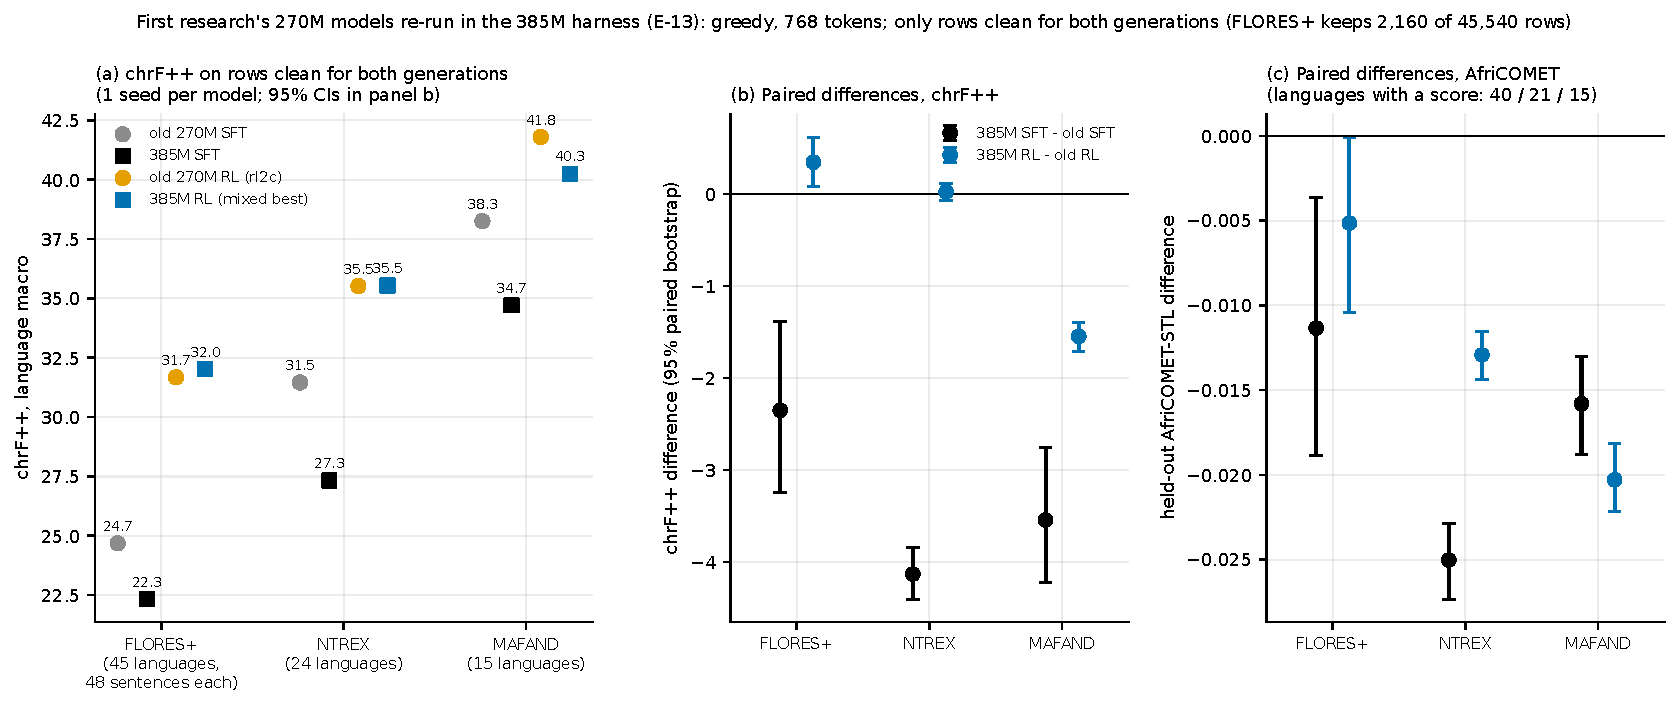
\includegraphics[width=1.00\linewidth]{figures/fig10_old270m_same_harness.pdf}
\caption{The earlier 270M work's 270M models re-run in the 385M harness (E-13): (a) language-macro chrF++ of the old 270M SFT and RL-final (rl2c) and the 385M SFT and RL (mixed best) on FLORES+ devtest (45 languages, 48 sentences each), NTREX (24) and MAFAND (15), rows clean for both generations only; (b) paired differences with 95\% bootstrap over sentences (Poisson weights; 1,000 resamples); (c) the same for held-out AfriCOMET-STL (languages with a score: 40 / 21 / 15). One seed per model. Source: \texttt{reports/\allowbreak{}data/\allowbreak{}e13\_\allowbreak{}old270m\_\allowbreak{}same\_\allowbreak{}harness\_\allowbreak{}2026-\allowbreak{}11-\allowbreak{}04/\allowbreak{}evidence\_\allowbreak{}e13.\allowbreak{}json}.}\label{fig:fig10_old270m_same_harness}
\end{figure}

\subsection{Weak and added languages}\label{app:weaklangs}

After SFT, 37 of 74 scored languages are weak (chrF++ < 14 or finished rate < 0.9), 16 of them by chrF++: shi 0.2, ibb 2.3, zgh 2.3, dag 2.4, aeb 2.8, taq 2.8, dik 3.8, knc 3.8, arz 4.6, ary 4.6, dyu 9.9, tir 10.5, cjk 10.7, orm 12.1, tiv 13.3, nus 13.5. Of the nine languages that the SFT report lists as added (the eight on FLORES+ that are among the 40 registry rows appended after A0, plus seh, which the registry counts among the first 85 rows), mfe (28.5) and seh (21.7) work, cjk (10.7) is weak, and arz, ary, dik, aeb, taq and zgh fail (English or Modern Standard Arabic output, token loops).  After RL (mixed best): mfe 37.93, cjk 23.02, dik 14.06, taq 11.06, arz 9.18, ary 6.88, aeb 4.12, zgh 4.07.  Arabic dialects, Tamazight, Dinka, Tamasheq and Kanuri (knc) are not usable after RL (chrF++ 2 to 14; loops in 11\% to 56\% of FLORES+ outputs by the reward's flag, and an English-output share of up to 0.5 in aeb and ary, Section~\ref{sec:degen}).
% src: EVAL section 6, T5
% src: EVID Table 6

\begin{figure}[t]
\centering
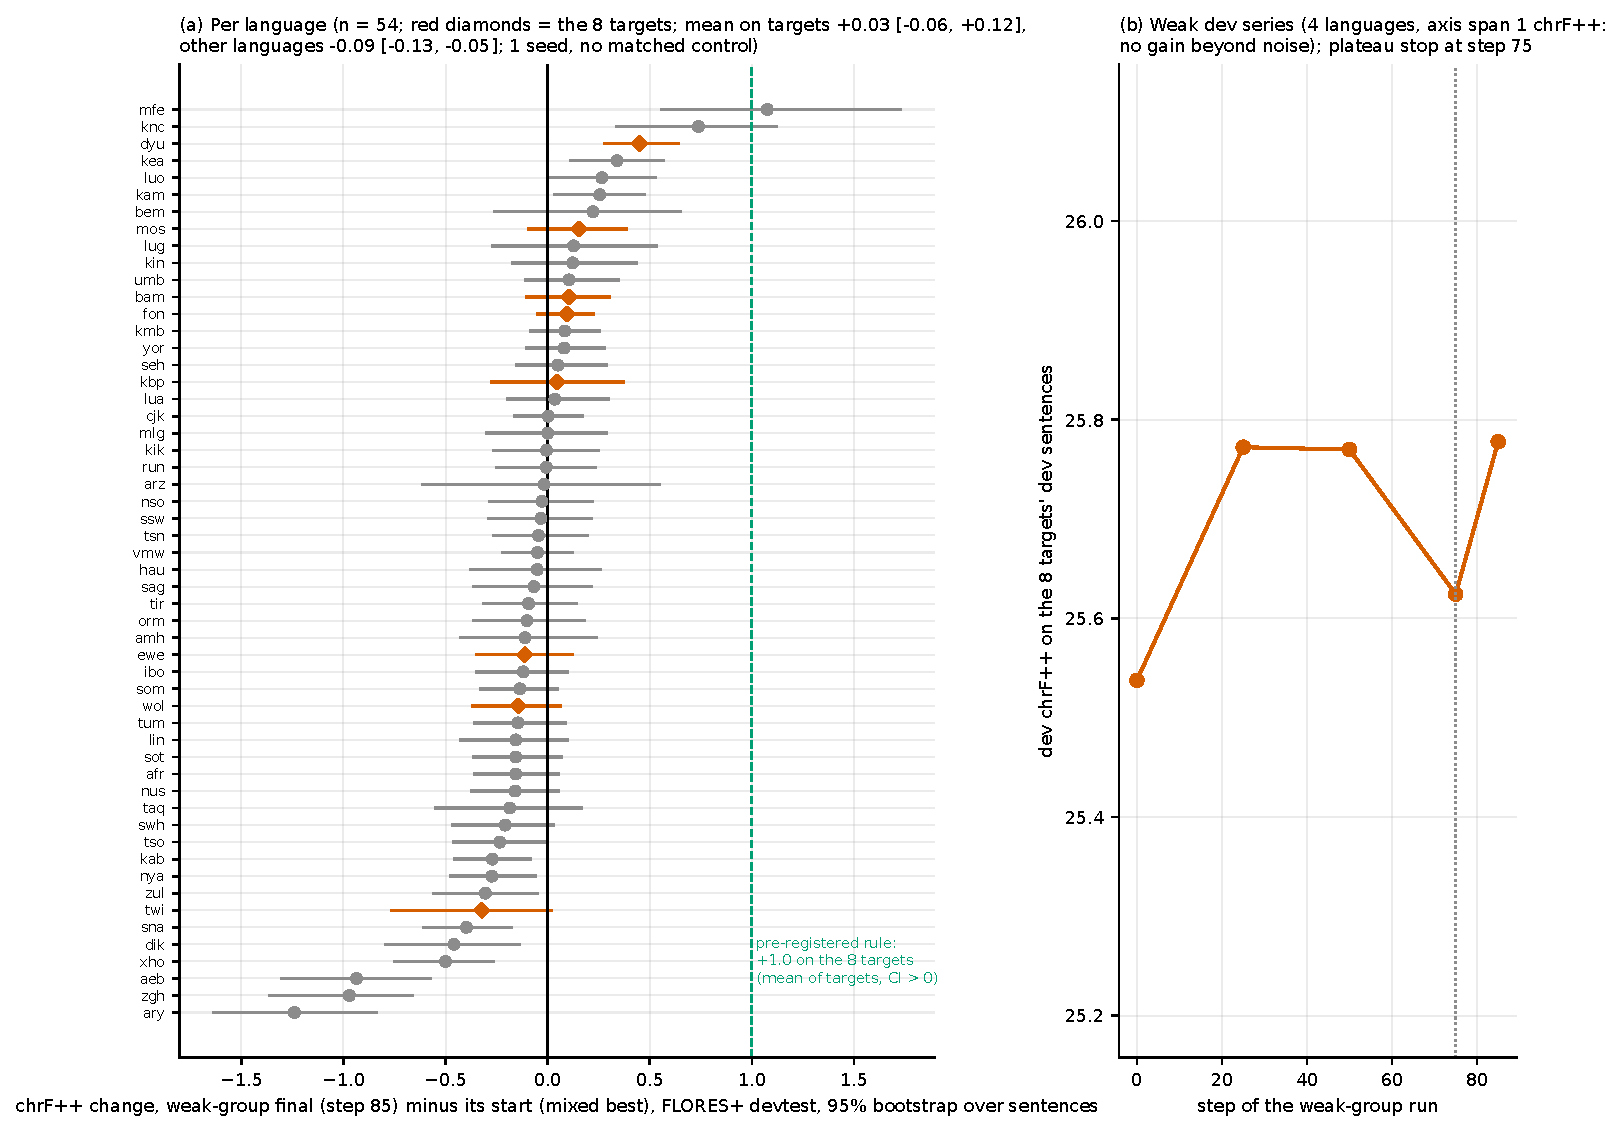
\includegraphics[width=0.90\linewidth]{figures/fig6_weak_group.pdf}
\caption{(a) Continued RL on eight weak West-African languages (mos fon kbp bam wol ewe twi dyu; 85 steps, 2.1 GPU-hours): chrF++ change of the final (step 85) against its start, the mixed best, per FLORES+ language (n = 54; 1,012 sentences each; 95\% bootstrap over sentences; one seed, no matched control). Red diamonds are the targets: mean +0.03 [\ensuremath{-}0.06, +0.12] against the pre-registered +1.0; the 46 other languages move by \ensuremath{-}0.09 [\ensuremath{-}0.13, \ensuremath{-}0.05]. (b) The run's own dev series on the targets' dev sentences (axis span 1 chrF++; dev evaluation noise is sd 0.09 to 0.10). Sources: \texttt{reports/\allowbreak{}data/\allowbreak{}eval\_\allowbreak{}weak\_\allowbreak{}group\_\allowbreak{}2026-\allowbreak{}11-\allowbreak{}03/\allowbreak{}scores/\allowbreak{}bootstrap\_\allowbreak{}by\_\allowbreak{}language.\allowbreak{}csv}, \texttt{research\_\allowbreak{}archive\_\allowbreak{}2026-\allowbreak{}11-\allowbreak{}03/\allowbreak{}clean\_\allowbreak{}rerun\_\allowbreak{}misc/\allowbreak{}runs\_\allowbreak{}385m\_\allowbreak{}weak/\allowbreak{}mixed/\allowbreak{}metrics.\allowbreak{}jsonl}.}\label{fig:weakgroup}
\end{figure}

\section{RL chain: stage summary, B1 final and training records}\label{app:chain}

\begin{table}[t]
\centering\scriptsize
\setlength{\tabcolsep}{4pt}
\caption{Stage chain summary (not all rows are FLORES+ stages).}\label{tab:chain_full}
\begin{tabularx}{\linewidth}{@{}>{\raggedright\arraybackslash}X>{\raggedright\arraybackslash}X>{\raggedright\arraybackslash}X>{\raggedright\arraybackslash}X@{}}
\toprule
stage & steps run & cost & result on FLORES+ chrF++ (vs previous stage) \\
\midrule
SFT-1 / SFT-2 (A0 $\to$ 385M) & 1,500 + 31,353 & 44.8 h for stage B (A100) & 22.85 (SFT, 54 languages) \\
continued-SFT control (E-03; not an RL stage) & 6,000 & 8.4 h (5.05 s/step), RL chain 8.66 h & FLORES+ 25.38 (+2.53 over the SFT [+2.35, +2.71]); 93 cells 29.97 against 34.55 for the mixed best \\
RL stage A & 400 & 15,920 s (4.42 h) & 30.81 (+7.96) \\
RL B1 & 135 (best step 50) & 10,479 s & 31.35 (+0.54) \\
RL mixed & 60 & 4,786 s & 31.66 (+0.31) \\
weak-group RL (8 languages) & 85 (plateau stop at 75) & 2.1 GPU-h & targets +0.03 [\ensuremath{-}0.06, +0.12]; other languages \ensuremath{-}0.09 [\ensuremath{-}0.13, \ensuremath{-}0.05] \\
science SFT & 283 (65,536 tokens) & 17 min & AfriScience chrF +1.2; SSA-COMET-QE flat \\
science RL & 160 steps executed (cap 150 in the yaml, extended to 190 at step 120; dev plateau at step 150 plus 10 wind-down steps; \texttt{summary.\allowbreak{}json} stop reason \texttt{dev\_\allowbreak{}plateau}; best at step 75) & not stated in the evaluation report & AfriScience test (6 languages), final vs start: chrF +0.46 [+0.27, +0.65], held-out AfriCOMET +0.0053 [+0.0036, +0.0071], SSA-COMET-QE +0.0041 (reward family); NTREX +0.42, MAFAND +0.10 chrF++; no document-level gain (not a FLORES+ stage) \\
science RL without the science SFT (E-14) & 160 (150 + 10 wind-down; one OOM restart from step 20; final only) & about 5 h wall-clock (15:18 to 20:17 UTC; 14,395 s in the last process) & AfriScience test chrF 45.66 (start 45.40; science RL from the science SFT 47.10); 93-cell chrF++ +0.13 over the mixed best (not a FLORES+ stage) \\
long-document RL & 80 (best at step 50; no extension) & 7.7 h wall-clock, of which about 4.5 h a crash loop (Appendix~\ref{app:repro}) & whole-document finished +0.125, loop \ensuremath{-}0.113, chrF +3.4; chunked and sentence level unchanged (not a FLORES+ stage) \\
\bottomrule
\end{tabularx}
\end{table}

% GATE E-03: the cost column is the compute the control must match
% src: reports/rl_vs_sft_evidence_2026-11-04.md section 6 (cost); EVID Table 3; reports/eval_weak_group_385m_2026-11-03.md; reports/eval_science_sft_385m_2026-11-04.md; LDOC section 2 (planned values). Science RL length: the yaml labels 150 steps a HARD CAP, but `extend_if_improving` (the trainer's extension rule: at the cap, if the improvement criterion fired within the last `extend_recent` steps, raise the cap) raised it by 40 steps to 190 while the dev metrics were still improving; the long-document yaml sets `extend_if_improving: false`. The stage A to mixed yamls also carry the extension rule (extend_steps 15, at most +50%). The executed count is reported from the run log and must be confirmed from `summary.json` when the run ends. The RL chain A + B1 + mixed is 8.66 A100-hours, of which B1's 85 steps after its best checkpoint are unused by the final model

 Stage A accounts for 94\% of the SFT-to-B1 gain on FLORES+ (7.96 of 8.50) and 96\% on NTREX; it also accounts for most of the improvement in finishing and looping (FLORES+ finished 0.829 $\to$ 0.983, loop 0.209 $\to$ 0.068; final 0.995, 0.048; Section~\ref{sec:rlsft}). We did not split the part beyond finishing by stage. The stage-A dev chrF++ (720 sentences) moves 36.81 $\to$ 39.04 (step 50) $\to$ 40.14 (100) $\to$ 40.47 (200) $\to$ 40.50 (400), with +3.3 of +3.7 in the first 100 steps; the plateau begins before the three KL-guard cuts (steps 226, 236, 247).  The later stages differ from stage A in more than step count (bin, reference domain, guides), and the later steps are small. Two extra seeds of the stage-A recipe (E-04, 100 steps, 20 languages, standard harness; Appendix~\ref{app:split}) differ by 0.06 chrF++ [\ensuremath{-}0.02, +0.14] (0.0008 AfriCOMET). On those 20 languages the stored B1 best is +0.17 [+0.12, +0.21] chrF++ over stage A, about three times the seed difference, while the mixed best is +0.07 [+0.02, +0.11] over B1 best, the size of the seed difference: \textbf{we do not call the mixed step a gain}; stage A to mixed is +0.23 [+0.18, +0.29]. These are indications from one pair of seeds at step 100, not tests of the later stages. 
% src: EVID Table 3; arithmetic checked in HYG X16
% src: STA; HYG X4
% src: reports/e04_rl_seeds_2026-11-05.md section 2; ledger E04 rows

\textbf{B1 best against B1 final (E-20).} The B1 final weights (step 135; \anonreal{an anonymised checkpoint}{Hub branch \texttt{stage-\allowbreak{}b1-\allowbreak{}final}}) were evaluated on the same 122,585 rows as every other stage (greedy, 768 tokens, language macro, 95\% paired bootstrap, one seed). 
% src: reports/e20_b1_final_2026-11-04.md; reports/data/e20_b1_final_2026-11-04/evidence_e20.json (ledger M8b)

\begin{table}[t]
\centering\footnotesize
\setlength{\tabcolsep}{4pt}
\caption{B1 final (step 135) against B1 best (step 50) and neighbouring stages; \chrfpp{}, language macro, 95\% paired bootstrap.}\label{tab:e20}
\begin{tabularx}{\linewidth}{@{}>{\raggedright\arraybackslash}Xllll@{}}
\toprule
comparison & FLORES+ chrF++ & NTREX chrF++ & MAFAND chrF++ & all 93 cells chrF++ \\
\midrule
B1 final minus B1 best & +0.04 [+0.00, +0.08] & \ensuremath{-}0.00 [\ensuremath{-}0.05, +0.05] & \ensuremath{-}0.09 [\ensuremath{-}0.15, \ensuremath{-}0.01] & +0.01 [\ensuremath{-}0.02, +0.04] \\
B1 final minus stage A & +0.58 [+0.53, +0.64] & +0.30 [+0.24, +0.36] & \ensuremath{-}0.09 [\ensuremath{-}0.17, +0.00] &  \\
mixed best minus B1 final & +0.26 [+0.22, +0.30] & +0.19 [+0.14, +0.23] & +0.05 [\ensuremath{-}0.01, +0.12] &  \\
\bottomrule
\end{tabularx}
\end{table}

Held-out AfriCOMET, B1 final minus B1 best, all cells: +0.0004 [+0.0000, +0.0008]; FLORES+ finished / loop 0.993 / 0.054 (B1 best) and 0.996 / 0.052 (B1 final). The 85 steps after step 50 changed nothing measurable, so the choice between B1 best and final does not matter for the numbers of this paper; 11 of 93 cells are significantly worse and 8 significantly better, by 0.1 to 0.3 chrF++, which is a rough noise floor for the stage-to-stage steps. (A table, not a figure, because the content is three differences.)

\begin{figure}[t]
\centering
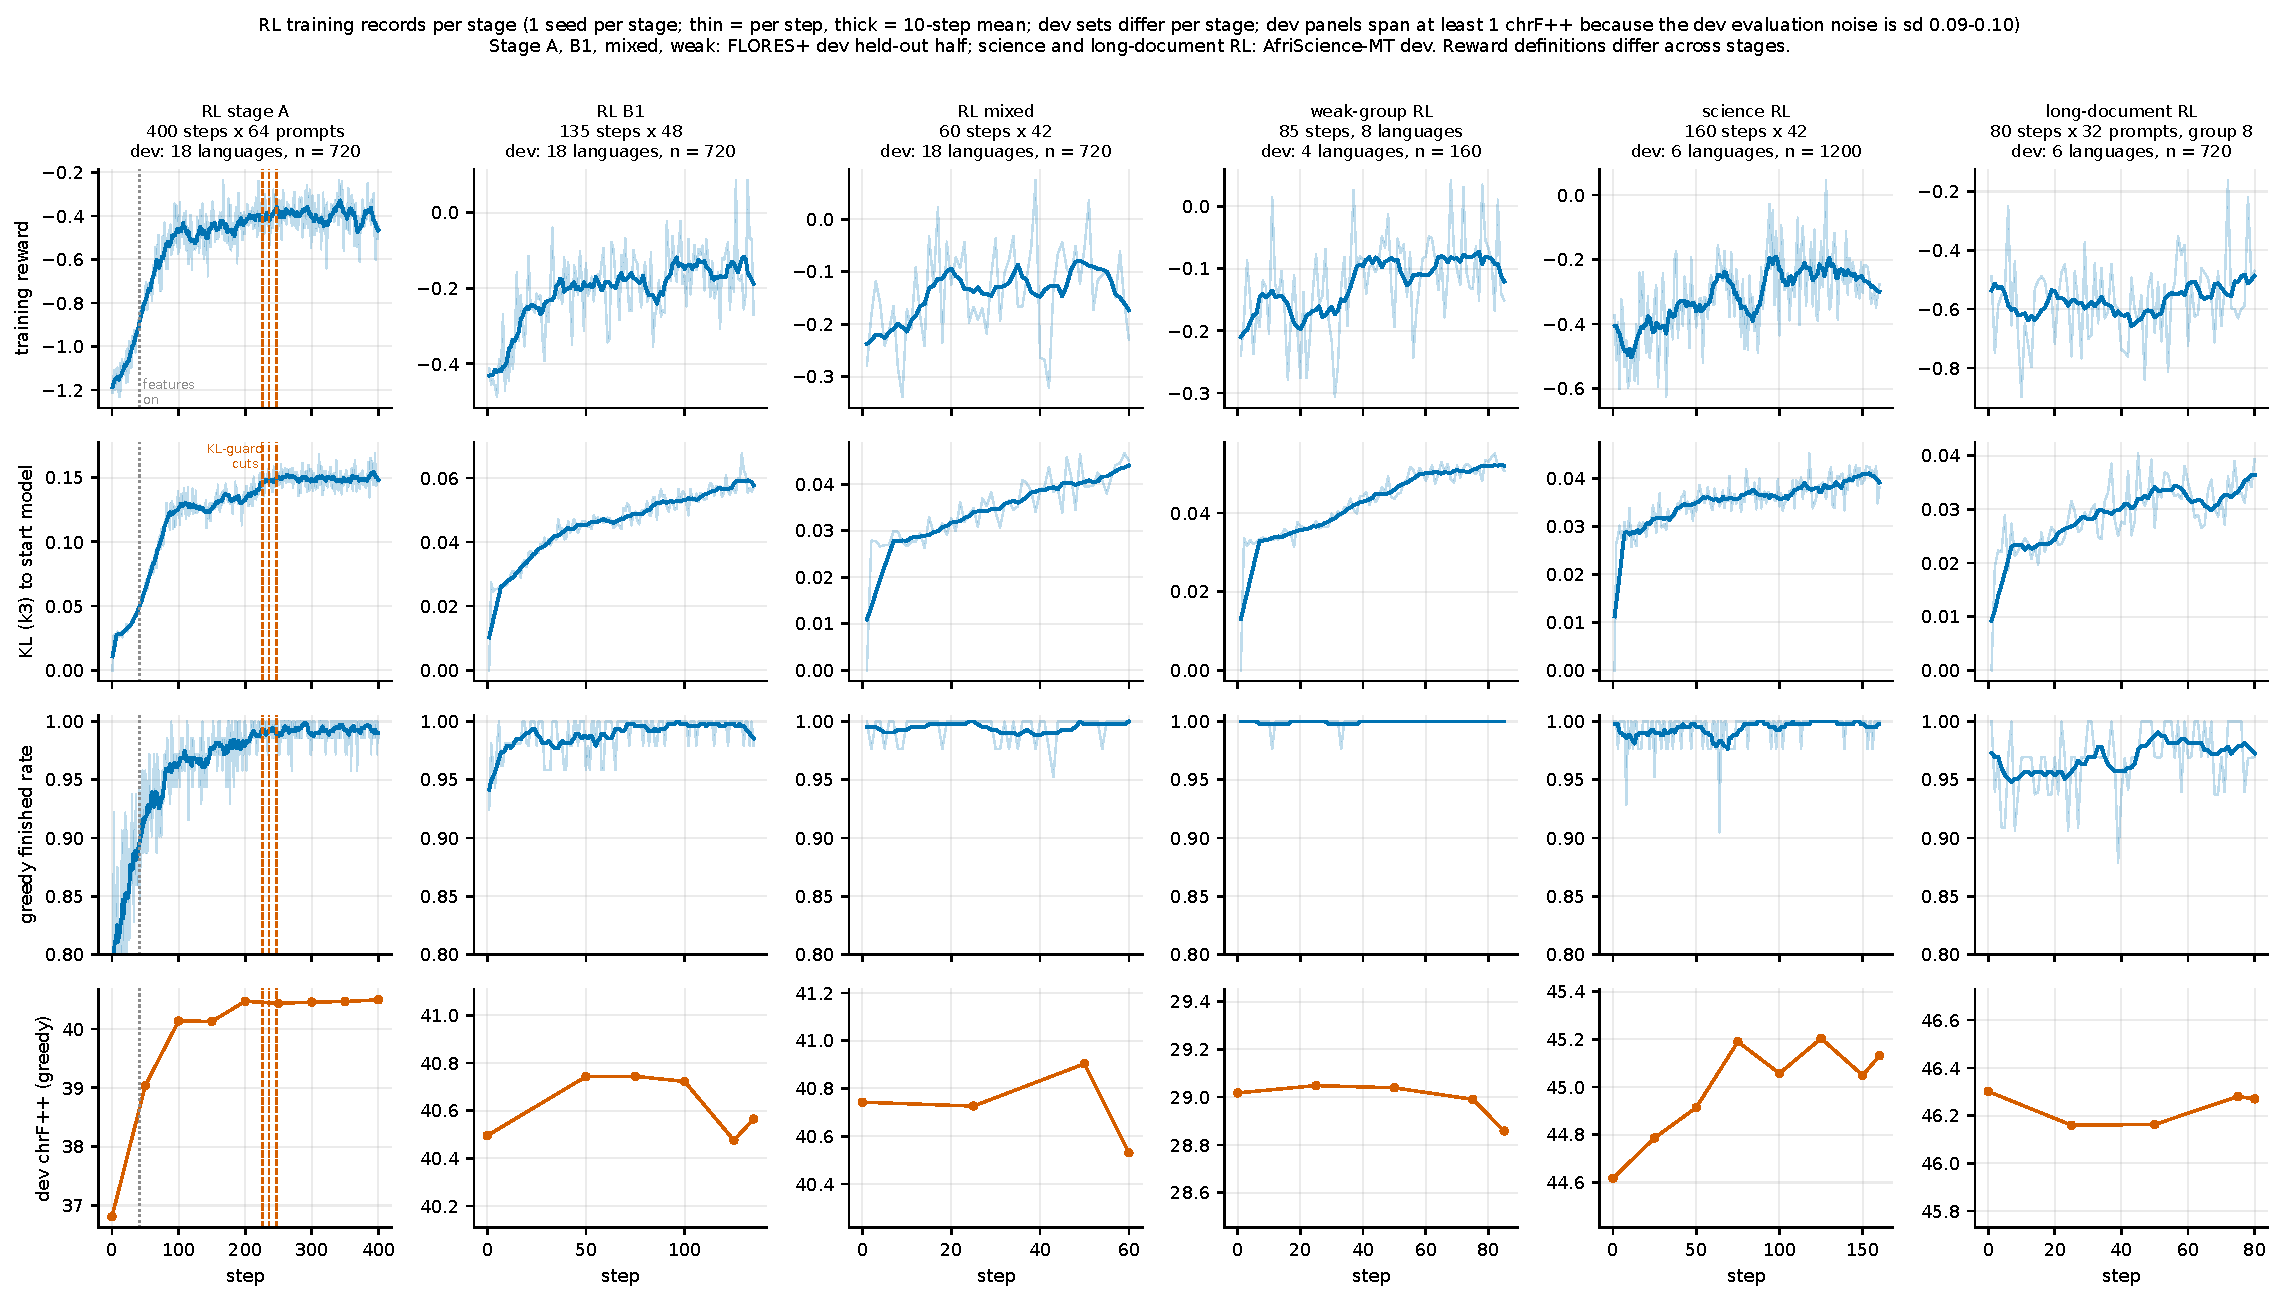
\includegraphics[width=1.00\linewidth]{figures/fig2_rl_training_curves.pdf}
\caption{Training records of every RL stage from the run logs (one seed per stage): training reward, KL (k3) to the stage's start model, finished rate of the greedy group member, and dev chrF++ against the step (thin lines per step, thick lines 10-step means). Stage A: dotted line at step 41 (four features on), dashed lines at the three KL-guard cuts (226, 236, 247). The dev sets differ by stage (FLORES+ dev held-out half for stage A, B1, mixed and weak; AfriScience-MT dev for science and long-document RL; the number of languages and sentences is in each title) and the reward definitions differ, so columns are not comparable; dev panels span at least 1 chrF++ because the dev evaluation noise is sd 0.09 to 0.10. The long-document RL log shows the 80 planned steps; step 25 was evaluated repeatedly after the crash restarts of Appendix~\ref{app:repro} and the last evaluation is shown (steps 21 to 25 were repeated by the restarts). Sources: \texttt{research\_\allowbreak{}archive\_\allowbreak{}2026-\allowbreak{}11-\allowbreak{}03/\allowbreak{}runs\_\allowbreak{}385m/\allowbreak{}\{A,B1,mixed\}/\allowbreak{}metrics.\allowbreak{}jsonl}, \texttt{clean\_\allowbreak{}rerun\_\allowbreak{}misc/\allowbreak{}runs\_\allowbreak{}385m\_\allowbreak{}\{weak/\allowbreak{}mixed,sci/\allowbreak{}final,long/\allowbreak{}final\}/\allowbreak{}metrics.\allowbreak{}jsonl}.}\label{fig:fig2_rl_training_curves}
\end{figure}

\section{RL against SFT and the control: details}\label{app:rlsft}

\begin{table}[t]
\centering\footnotesize
\setlength{\tabcolsep}{4pt}
\caption{Finished rate / loop rate (reward's flag) / hypothesis-to-reference length, clean rows, language macro.}\label{tab:finish}
\begin{tabularx}{\linewidth}{@{}l>{\raggedright\arraybackslash}Xll@{}}
\toprule
system & FLORES+ finished / loop / hyp-to-ref length & NTREX & MAFAND \\
\midrule
SFT & 0.829 / 0.209 / 3.03 & 0.890 / 0.122 / 2.35 & 0.963 / 0.043 / 1.48 \\
RL stage A & 0.983 / 0.068 / 1.33 & 0.996 / 0.016 / 1.07 & 0.999 / 0.003 / 1.00 \\
RL B1 best & 0.993 / 0.054 / 1.17 & 0.999 / 0.009 / 1.02 & 1.000 / 0.001 / 0.99 \\
RL mixed best & 0.995 / 0.048 / 1.14 & 0.999 / 0.006 / 1.02 & 1.000 / 0.001 / 0.98 \\
\bottomrule
\end{tabularx}
\end{table}

 The loop detector in this table is the reward's own guard (\texttt{is\_\allowbreak{}repetitive}, \texttt{is\_\allowbreak{}self\_\allowbreak{}repetitive}); on the human references it fires on 0.0001 of FLORES+ rows. 95\% of the RL model's flagged FLORES+ rows come from seven near-failed languages (taq knc zgh dik aeb arz ary). Section~\ref{sec:degen} tests this flag against a detector that is not the reward's.
% src: EVID Table 2

\begin{table}[t]
\centering\footnotesize
\setlength{\tabcolsep}{4pt}
\caption{RL minus SFT over the 93 cells under four ways of removing the finishing effect (clean rows; 95\% CI).}\label{tab:decomp}
\begin{tabularx}{\linewidth}{@{}>{\raggedright\arraybackslash}X>{\raggedright\arraybackslash}X>{\raggedright\arraybackslash}X@{}}
\toprule
row set & chrF++ RL - SFT [95\% CI] & AfriCOMET RL - SFT [95\% CI] (76 cells) \\
\midrule
all clean rows & +7.96 [+7.82, +8.12] & +0.0631 [+0.0620, +0.0643] \\
SFT output cut at its first loop (RL as is) & +4.06 [+3.97, +4.15] & not scorable \\
rows where the SFT finished and did not loop & +2.41 [+2.33, +2.49] & +0.0366 [+0.0357, +0.0374] \\
rows where both finished and neither loops & +2.61 [+2.54, +2.70] & +0.0370 [+0.0362, +0.0379] \\
rows where the SFT failed (21\% of FLORES+ rows) & +24.57 [+24.26, +24.90] (SFT 5.95, RL 30.53) & +0.3342 [+0.3295, +0.3391] \\
\bottomrule
\end{tabularx}
\end{table}

 Cutting the SFT's looping outputs at the loop onset (no change to the translation) raises the SFT from 26.59 to 30.49 chrF++, i.e. \textbf{49\% of the gain is recovered by cutting loops}; 67 to 70\% of the chrF++ gain is attributable to rows where either model failed; about 41\% of the AfriCOMET gain is finishing. What remains is +2.4 to +4.1 chrF++ and +0.037 AfriCOMET, significant in 50 of 54 FLORES+ languages on clean rows. The three estimates favour different models (the paired subset keeps only sentences the SFT can handle; the cut-at-loop rule is a heuristic) and agree in sign and rough size. The cut-at-loop rule is the reward family's loop rule; it was not redone with the independent detector of Section~\ref{sec:degen}. The decode-time guard control (E-01, below) answers the question this raises: a frequency penalty of 0.10 on the SFT recovers the same 49\% of the chrF++ gain (29\% of the AfriCOMET gain) without any RL, so the finishing share is a property of unguarded greedy decoding that the RL also repairs. Caveats: the guard setting was chosen on the FLORES+ dev held-out half by a rule fixed in advance and its optimum (0.10) lay at the edge of the grid, so the control may be under-tuned; a post-hoc dev-only extension to stronger penalties (SFT dev chrF++ 37.36 at 0.10, 37.97 at 0.20, 38.00 at 0.30, 38.25 at 0.50) was still rising and no full evaluation with a stronger penalty was run; one seed (\texttt{reports/\allowbreak{}e01\_\allowbreak{}loop\_\allowbreak{}guard\_\allowbreak{}2026-\allowbreak{}11-\allowbreak{}04.\allowbreak{}md}, \texttt{reports/\allowbreak{}overnight\_\allowbreak{}log\_\allowbreak{}2026-\allowbreak{}11-\allowbreak{}04.\allowbreak{}md} 09:00 row).
% src: EVID Table 1, section 3

Language-macro chrF++ per benchmark, SFT / control / mixed best: FLORES+ 22.85 / 25.38 / 31.66, NTREX 29.25 / 33.74 / 37.17, MAFAND 35.77 / 40.44 / 40.78; the control gains +2.53 [+2.35, +2.71], +4.49 [+4.29, +4.70] and +4.67 [+4.39, +4.92] over the SFT against +8.81, +7.91 and +5.01 for the RL; over the 93 cells it gains +3.38 against +7.96 (42.5\% of the SFT-to-RL gap, arithmetic of the macros). Held-out AfriCOMET: RL minus control is +0.0373 on FLORES+, +0.0051 on NTREX and \ensuremath{-}0.0141 on MAFAND (the last favours the control). Finished and loop rates (the reward's flag) on FLORES+, SFT / control / mixed best: 0.829 / 0.854 / 0.995 and 0.209 / 0.178 / 0.048; by panel (FLORES+ finished): the 19 TranslatePsy languages 0.931 / 0.993 / 1.000, the other languages 0.774 / 0.779 / 0.993. The independent degeneration detector gives the same picture (FLORES+ flag 0.311 for the SFT, 0.268 for the control, 0.085 for the mixed best). \textbf{The control repairs finishing and looping only on the languages it was trained on}, where it comes close to the RL model; on the other languages it changes almost nothing (+0.15 chrF++ over the SFT on FLORES+ [\ensuremath{-}0.03, +0.32], 35 languages). 

\begin{table}[h]
\centering\small
\caption{The pre-registered decision rule applied to mixed best against the 6,000-step control.}\label{tab:e03rule}
\begin{tabular}{@{}llc@{}}
\toprule
registered condition & value & met\\
\midrule
lower 95\% bound of $d$ (\chrfpp{}, 93 cells) $>+1.0$ & $+4.58$ \ci{+4.45}{+4.70} & yes\\
lower bound of the AfriCOMET difference $>0$ & $+0.0183$ \ci{+0.0172}{+0.0192} & yes\\
$d>0$ on the 19 TranslatePsy languages & $-0.03$ \ci{-0.13}{+0.09} & \textbf{no}\\
$d>0$ on the other languages & $+9.29$ \ci{+9.09}{+9.49} & yes\\
\bottomrule
\end{tabular}
\end{table}

\textbf{By the rule as registered the verdict is ``inconclusive''}, because the condition on the 19 TranslatePsy languages is not met (d = \ensuremath{-}0.03); the other three are. We did not change the rule. Reading the panels: where a teacher-translated corpus exists continued SFT matches RL in chrF++ and largely fixes finishing and looping, and the control is ahead of RL on the neural metrics there; RL's advantage is that it improves every language from its own samples and a QE reward, including those for which no such corpus was used (+9.29 on 46 cells). A reader who takes the overall endpoint alone gets ``RL is better'' (+4.58 [+4.45, +4.70], above the +1.0 margin, AfriCOMET above 0); a reader who takes the 19 languages alone gets ``comparable'' in chrF++ (interval inside $\pm$1.0) but not by the registered rule (the AfriCOMET interval excludes 0 in favour of the control); neither is the registered verdict. On AfriScience-MT test sentences (6 languages) the control scores chrF 44.71 against 45.40 for the mixed best and 36.00 for the SFT, and is ahead of the RL on SSA-COMET-QE (0.6214 against 0.6130) and AfriCOMET (0.6947 against 0.6828), the metrics in the family that filtered TranslatePsy; nso, the one of the six languages without TranslatePsy data, stays at the SFT level for the control (41.27 $\to$ 40.64) while the RL gains 10.9.

Caveats. One seed, \textbf{one learning rate} (the probe's best of three) and \textbf{one evaluated budget point}: the stage-A-matched (3,100 steps) and mixed-best-matched (4,800 steps) comparisons are untested, and a different mix, schedule or longer run could change the control. Differences below about 0.5 chrF++ are inside the unmeasured seed variation. The control is not information-matched: it receives NLLB-3.3B translations (a teacher that scores 38.80 against 26.30 for the SFT on 43 languages, Section~\ref{sec:nllb}) for 19 languages that the RL never sees, and the TranslatePsy rows were filtered with AfriCOMET, SSA-COMET and MetricX, so those neural metrics favour the control; chrF and chrF++ are the evidence. The control's loop count is undercounted by the reward's flag too (independent / reward flag 1.51 on FLORES+). TranslatePsy is CC-BY-NC-4.0 with NLLB-derived targets and was used only for this control; nothing of it is in any released model, and the control checkpoint is not released (Appendix~\ref{app:disc}). 
% src: reports/e03_sft_control_2026-11-05.md sections 1, 3, 4; ledger R14, CTL7-CTL11

\section{Independent degeneration audit: details}\label{app:degenapp}

The reward's loop flag is the guard the RL was optimised against, so a loop type it misses would be undercounted for the RL. We re-measured with a detector that shares the idea (repetition) but none of the code or constants: the lzma-compressed size of the output relative to what human references of the same benchmark, language and length would give, the share of repeated character 8-grams and the share of repeated word 3-grams, each threshold set so that 0.1\% of the 122,585 human references fire it. Rows are all rows of FLORES+ (54 languages), NTREX (24) and MAFAND (15) for each system, no clean-row filter.  
% src: DEGEN section 2 Table; `reports/data/degeneration_audit_independent_2026-11-04/summary_by_model_benchmark.csv`, `bootstrap_rates.csv`. DEGEN uses all rows while EVID Table 2 uses clean rows; the reward-flag values agree to the three decimals quoted in EVID (0.209/0.048, 0.122/0.006, 0.043/0.001)

\begin{table}[t]
\centering\footnotesize
\setlength{\tabcolsep}{4pt}
\caption{Loop flag of the reward against the independent detector, language macro (95\% bootstrap in brackets).}\label{tab:degen}
\begin{tabularx}{\linewidth}{@{}lrrl>{\raggedright\arraybackslash}X@{}}
\toprule
system & FLORES+ reward flag & FLORES+ independent flag & NTREX reward / independent & MAFAND reward / independent \\
\midrule
SFT & 0.2095 & 0.3107 [0.3029, 0.3190] & 0.1218 / 0.1662 & 0.0431 / 0.0754 \\
RL stage A & 0.0675 & 0.1207 [0.1160, 0.1253] & 0.0165 / 0.0309 & 0.0026 / 0.0092 \\
RL B1 best & 0.0541 & 0.0980 [0.0942, 0.1019] & 0.0092 / 0.0190 & 0.0013 / 0.0056 \\
RL mixed best & 0.0480 [0.0462, 0.0496] & 0.0851 [0.0822, 0.0883] & 0.0064 / 0.0143 & 0.0009 / 0.0039 \\
human references & 0.0001 & 0.0018 & 0.0000 / 0.0018 & 0.0000 / 0.0013 \\
\bottomrule
\end{tabularx}
\end{table}

\begin{itemize}
\item \textbf{The reward's flag is a lower bound.} On mixed-best FLORES+ the independent detector flags 1.77 [1.71, 1.84] times as many outputs as the reward's flag (NTREX 2.25 [1.95, 2.59], MAFAND 4.42 [3.14, 7.29] on tiny base rates). At a ten times stricter threshold (0.01\% of references) the FLORES+ rates are 0.0586 against 0.0480 (ratio 1.22), so the excess is not an artefact of a loose threshold. The undercount is present for the SFT too (ratio 1.48), so it enters the RL-versus-SFT comparison only through 1.48 against 1.77; the reduction of the loop rate from SFT to RL is 3.7x with the independent detector and 4.4x with the reward's.
\item \textbf{The extra rows are finished partial repetitions and cost little.} Of 122,585 mixed-best rows, 2,932 are flagged by both, 14 by the reward only and 2,488 by the independent detector only. The independent-only rows are 99.9\% finished, have a median of 26 words and 48\% of them are in the seven near-failed languages. Hard failures are caught by both (of 278 unfinished rows 2 escape the reward's flag and none the independent one). If the independent-only rows scored the average of the unflagged rows of their language, the macro chrF++ of the mixed best would rise by 0.19 (FLORES+), 0.02 (NTREX) and 0.015 (MAFAND), against 0.46, 0.28 and 0.23 for the SFT. The difference between SFT and RL in this loss is 0.26, 0.26 and 0.22 chrF++, i.e. 3.0\%, 3.3\% and 4.4\% of the RL gains (+8.81, +7.91, +5.01) by arithmetic. \textbf{The decomposition above does not change materially.} 
% src: DEGEN section 0, `crosstab_reward_vs_independent.csv`, `chrf_loss_attributable_to_independent_only_rows.csv`. The language-matched chrF++ of independent-only rows is 4.54 below that of unflagged rows (se 0.51; 39 of 44 languages) but this is selection-confounded (hard sentences repeat more). DISAGREEMENT FLAG: the report's "3 to 4%" rounds 4.4% down; use the three percentages
\item \textbf{Length and tails.} Median hypothesis-to-reference character ratio is 1.02 to 1.07 for all systems. The share of FLORES+ outputs longer than twice the reference falls from 0.2005 (SFT) to 0.0281 (mixed best). Of the 2,079 mixed-best rows above 2x, 24.5\% (about 0.4\% of all rows) are finished and flagged by neither detector: long, non-repetitive continuations that no repetition rule sees. Unterminated tails on FLORES+ fall from 0.1847 to 0.0464 against 0.0162 for human references; NTREX and MAFAND are at or below the reference rate. 
% src: DEGEN sections 3, 4
\item \textbf{Language.} An independent language-identification model (NLLB-218, reliable for 40 of the evaluated languages) agrees with the reward's GlotLID: FLORES+ pass rate SFT 0.9487, mixed best 0.9669 (references 0.9915); GlotLID 0.9098 and 0.9553. On mixed-best FLORES+ 0.86\% of the rows GlotLID passes fail the NLLB LID, so the language guard's pass rate is not inflated by optimisation. The LID is blind to the weakest languages (none for aeb ary arz mfe nde seh shi ven vmw; unreliable for nine more). 
% src: DEGEN section 6
\end{itemize}

 Four languages account for 96\% of the macro increase (human references: 0.0004); GlotLID gives the same numbers within 0.005. These languages, with taq, dik and knc, are outside the RL prompt pool, and the model emits the tag of a sibling language (\texttt{<arz>} for ary and half of aeb, \texttt{<tzm>} for zgh and taq). The reward's copy guard sees only 0.086 of aeb and 0.064 of ary outputs. So part of the ``RL loops less'' gain in these languages is a change from loops to English output, while their chrF++ stays at 2 to 9.
% src: DEGEN section 5, `arabic_tifinagh_english_leak.csv`
\begin{itemize}
\item \textbf{What the audit does not establish.} There is no ground truth for ``degenerate''; the detector is validated by the reference control, by reading 25 mixed-best and 12 SFT examples, and by the lower language-matched chrF++. It is blind to non-repetitive failures (hallucination, wrong content) except through the length audit. The NLLB LID is licensed cc-by-nc-4.0 and was used for evaluation only.
\end{itemize}

The share of outputs identified as English (NLLB-218 top-1, $p\ge0.5$) on FLORES+ by system:

\begin{table}[t]
\centering\small
\setlength{\tabcolsep}{4pt}
\caption{Share of FLORES+ outputs identified as English, by system.}\label{tab:english}
\begin{tabularx}{\linewidth}{@{}>{\raggedright\arraybackslash}Xrrrrr@{}}
\toprule
language & SFT & stage A & B1 best & mixed best & weak final \\
\midrule
aeb & 0.215 & 0.400 & 0.397 & 0.449 & 0.498 \\
ary & 0.041 & 0.275 & 0.339 & 0.394 & 0.488 \\
arz & 0.006 & 0.059 & 0.075 & 0.098 & 0.151 \\
zgh & 0.001 & 0.017 & 0.029 & 0.049 & 0.074 \\
macro, 54 languages & 0.0055 & 0.0146 & 0.0164 & 0.0191 & 0.0235 \\
\bottomrule
\end{tabularx}
\end{table}

\section{Stage-A log analysis and ablation details}\label{app:split}

\textbf{The stage-A log cannot separate the four features (E-11 can).} Stage A steps 1-40 ran without the four features and steps 41-400 with them. An earlier note said the KL slope ``tripled'' when the features began (0.00053 per step over steps 2-40, 0.00143 over steps 41-100). Reading the log: both numbers reproduce exactly, \textbf{but the factor is 2.0, not 3}: the first segment contains the learning-rate warm-up (steps 1-10); from step 11 the pre-feature slope is 0.00070 [0.00061, 0.00079] and 0.00143/0.00070 = 2.0. The KL was also already accelerating before step 41 (slopes over 15-step windows: 0.00048 for steps 11-25, 0.00101 for 26-40, 0.00158 for 41-55), the curve is smooth through step 41 with no kink, and it saturates by step \textasciitilde\{\}90 (flat at 0.124 to 0.129 until step \textasciitilde\{\}160). A power-law extrapolation of the pre-feature trend predicts a KL of 0.042 to 0.065 at step 100 against 0.131 observed, so the acceleration is faster than the extrapolated trend, but that is a statement about extrapolating 30 to 40 noisy points, not an identification of a cause. 
% src: SPLIT sections 1-2; ledger R17

\textbf{Nothing else accelerates at step 41.} The per-step slopes of the training reward (+0.0065 [0.0051, 0.0079] before, +0.0071 [0.0060, 0.0080] after), of the finished rate, of the greedy loop rate (\ensuremath{-}0.0020 before, \ensuremath{-}0.0011 after) and of the hard-fail share (\ensuremath{-}0.00138 before, \ensuremath{-}0.00040 after) are the same or steeper before step 41, because the failure rates were high and floor out. An interrupted-time-series fit finds level shifts at step 41 (KL +0.0086 [0.0021, 0.0149], reward +0.093 [0.041, 0.147], greedy loop rate \ensuremath{-}0.028 [\ensuremath{-}0.052, \ensuremath{-}0.004], hard-fail share \ensuremath{-}0.014 [\ensuremath{-}0.026, \ensuremath{-}0.003]), but the reward and the finished and loop rates are not the same quantity before and after step 41 (from step 41, 15\% of the prompts carry the reference term and 25\% of the groups contain the guide), and the shifts could equally be a resume artefact (checkpoint reload, RNG, a fresh prompt stream). They say ``something changed at 41 on top of the trend'', not which feature did it. The dev curve is evaluated only at steps 0, 50, ..., 400, so no dev point separates steps 1-40 from 41-50. 
% src: SPLIT section 2; ledger R18

\textbf{Which feature could act at all.} Dynamic sampling never acted (flat-group fraction 0, no refill) and the std floor never bound (group-std p10 0.128 against 0.02), so any effect at step 41 could only come from the beam guide, the reference domain or the resume itself; the log could not say which. We therefore ran the ablations (below).

\textbf{Seed spread (E-04).} Two extra runs of the stage-A recipe (seeds 20261105 and 20261106; 100 steps; the executed stage A used seed 1234, so the three runs share the recipe, the SFT start and the 40-step feature-free prefix schedule) were evaluated with the standard harness on 20 languages (yor hau ibo swh amh zul xho kin som wol lug sna twi ewe lin tir orm nso tsn afr; FLORES+, NTREX, MAFAND; 49 cells; greedy, 768 tokens). Gains over the SFT are +5.96 [+5.80, +6.11] and +5.90 [+5.74, +6.05] chrF++ (+0.0462 and +0.0454 AfriCOMET): the two seeds differ by \textbf{0.06 chrF++ [\ensuremath{-}0.02, +0.14]} (0.0008 AfriCOMET; per language they differ significantly in 2 of 20, by at most 0.54). The in-training dev gains of the three runs are +3.33, +3.70 and +3.46 (the dev subset depends on the seed, so only gains over each run's own step 0 are compared). The stage-A gain is therefore reproducible across training seeds at step 100, and per-language differences below about 0.5 chrF++ are not separable from training noise. \textbf{This is one pair of seeds at step 100, not a seed study of later stages}; the 400-step stage A is +0.78 [+0.70, +0.86] and +0.84 [+0.75, +0.92] above the 100-step seeds on the same cells. 
% src: reports/e04_rl_seeds_2026-11-05.md sections 1-3 (ledger E04 rows)

\textbf{Ablations (E-11).} Arms (a) no features, (c) no reference domain (no reference prompts and no reference-anchored reward) and (d) no beam guide were run for 100 steps (b64 recipe, one run per arm) as forks of seed 2's step-40 state, so arm minus seed 2 is a tight paired comparison and arm minus seed 3 carries the full seed noise; arm (b), the full set, is the two seeds. Pre-registered rule: an effect is real if the paired interval excludes 0, its size exceeds the observed seed difference (0.06) and AfriCOMET does not point the other way. 

\begin{table}[t]
\centering\footnotesize
\setlength{\tabcolsep}{4pt}
\caption{Ablation arms at 100 steps, \chrfpp{} over 49 cells (20 languages); arm minus the full-feature seed 2 (paired) and minus seed 3 (E-11).}\label{tab:e11}
\begin{tabularx}{\linewidth}{@{}llll>{\raggedright\arraybackslash}X@{}}
\toprule
arm & chrF++ (49 cells) & arm minus seed 2 & arm minus seed 3 & AfriCOMET vs seed 2 \\
\midrule
(b) full, seed 2 & 38.51 [38.30, 38.69] & - & - & - \\
(b) full, seed 3 & 38.46 [38.26, 38.64] & - & - & - \\
(a) no features & 38.19 [37.99, 38.38] & \ensuremath{-}0.32 [\ensuremath{-}0.41, \ensuremath{-}0.23] & \ensuremath{-}0.26 [\ensuremath{-}0.35, \ensuremath{-}0.18] & \ensuremath{-}0.0028 [\ensuremath{-}0.0033, \ensuremath{-}0.0022] \\
(c) no reference domain & 38.35 [38.16, 38.54] & \ensuremath{-}0.16 [\ensuremath{-}0.25, \ensuremath{-}0.08] & \ensuremath{-}0.10 [\ensuremath{-}0.19, \ensuremath{-}0.02] & \ensuremath{-}0.0017 [\ensuremath{-}0.0023, \ensuremath{-}0.0011] \\
(d) no beam guide & 38.42 [38.23, 38.61] & \ensuremath{-}0.09 [\ensuremath{-}0.17, \ensuremath{-}0.01] & \ensuremath{-}0.04 [\ensuremath{-}0.11, +0.04] & \ensuremath{-}0.0005 [\ensuremath{-}0.0010, +0.0001] \\
\bottomrule
\end{tabularx}
\end{table}

Removing all four features costs \textbf{0.32 chrF++ [0.23, 0.41]} (about five times the seed difference; consistent on the three benchmarks, AfriCOMET and the loop flag), about 5\% of the 5.96 chrF++ gain, and it does not show on the in-training dev macro (\ensuremath{-}0.14 [\ensuremath{-}0.51, +0.25]). Removing the reference domain costs 0.16 [0.08, 0.25] (real by the rule against seed 2, 2.7 times the seed difference): about half of the feature set's effect. Removing the beam guide costs 0.09 against seed 2 but 0.04 [\ensuremath{-}0.04, +0.11] against seed 3 with AfriCOMET inside noise: \textbf{not separable from seed noise}, for about +25\% step time (median step 40.3 s with the guide against 32.4 s without). Dynamic sampling and the std floor never acted and are part of arm (a) only. \textbf{The KL rise is not caused by the features:} the median KL of steps 81 to 90 is 0.116 without any feature, 0.122 without the reference domain, 0.120 without the guide and 0.123 and 0.120 for the two full runs, and the same holds at steps 51 to 60 (0.075, 0.0745, 0.073, 0.072, 0.073). \textbf{The earlier inference that the beam guide drives the KL slope (stage report, ledger M10) is therefore not supported}; the step-41 acceleration seen in stage A is at most a small effect. Arm (e) (KL guard 0.25 against 0.15) was not run by the pre-registered rule, because the guard never fired in any of the 100-step runs (maximum 5-step median KL 0.120 to 0.127 against 0.15). Caveats: one run per arm, a shared 40-step prefix with seed 2, one pair of seeds as the noise yardstick (so the ``real'' rule is lenient and effects of 0.1 to 0.2 chrF++ are small and suggestive), 100 steps and 20 languages only (the reference domain covers amh efi hau lug nso yor zul, five of them in these 20). \textbf{Reading:} the four features are design choices with a small measured benefit (+0.3 chrF++ at 100 steps, mostly the reference-anchored term), not the source of the RL gain, and the beam guide is not shown to be worth its generation time. 
% src: reports/e11_rl_ablations_2026-11-05.md sections 1-3 (ledger E11 rows, M10 corrected)

\section{Decoding and engine parity: details}\label{app:decoding}

\textbf{Earlier 256-token study (SFT only; superseded for beam).} 20 languages $\times$ 200 FLORES+ devtest sentences, 256-token cap. Its beam rows came from a vLLM beam loop that completes a beam only on the tokenizer's \texttt{<eos>}, not on \texttt{<end\_\allowbreak{}of\_\allowbreak{}turn>}, and ran every instance to the cap, so \textbf{its beam numbers are not comparable with the beam-4 of E-02 below} and are kept only as the record of what that study measured; its greedy and MBR rows are not affected by this. 
% src: EVAL section 1, T8; reports/e02_beam_mbr_768_2026-11-05.md Amendment 1 and section 4

\begin{table}[t]
\centering\footnotesize
\setlength{\tabcolsep}{4pt}
\caption{Earlier 256-token study (SFT only; 20 languages $\times$ 200 FLORES+ sentences). Beam rows are not comparable with E-02.}\label{tab:old256}
\begin{tabular}{@{}lrlrl@{}}
\toprule
decoding & chrF++ & delta vs greedy [95\% CI] & spBLEU & delta spBLEU \\
\midrule
greedy & 35.00 & - & 13.64 & - \\
beam 4 & 37.53 & +2.53 [+2.18, +2.87] & 16.38 & +2.73 [+2.39, +3.08] \\
MBR-16 (+ greedy) & 38.29 & +3.30 [+3.00, +3.58] & 15.30 & +1.65 [+1.38, +1.90] \\
\bottomrule
\end{tabular}
\end{table}

MBR minus beam is +0.76 [+0.49, +1.02] chrF++ and \ensuremath{-}1.08 [\ensuremath{-}1.39, \ensuremath{-}0.79] spBLEU; MBR uses chrF++ as its utility. The study's greedy is cap-protected (greedy on the same sentences is 32.50 at 768 tokens against 35.00 at 256), which is one more reason not to use its beam gain.

\begin{table}[t]
\centering\scriptsize
\setlength{\tabcolsep}{4pt}
\caption{E-02: greedy, beam-4 and MBR-16 at 768 new tokens, full table (20 languages, 4,000 sentences per system, 95\% paired bootstrap).}\label{tab:e02_full}
\begin{tabularx}{\linewidth}{@{}>{\raggedright\arraybackslash}Xllllll@{}}
\toprule
system & chrF++ & spBLEU & AfriCOMET-STL & finished & loop (independent) & output / reference length \\
\midrule
SFT greedy & 32.31 [31.43, 33.38] & 11.47 & 0.5513 [0.5403, 0.5621] & 0.915 & 0.147 & 2.05 \\
SFT beam-4 (stop at 4 ended) & 36.02 [35.13, 36.95] & 16.49 & 0.5639 [0.5521, 0.5750] & 1.000 & 0.108 & 0.96 \\
SFT beam-4 (HF early\_stopping=False) & 33.26 [32.22, 34.46] & 13.07 & 0.5722 [0.5603, 0.5845] & 0.897 & 0.139 & 2.15 \\
SFT MBR-16 (metric-matched) & 38.27 [37.60, 39.01] & 15.25 & 0.5780 [0.5687, 0.5870] & 0.9998 & 0.016 & 1.16 \\
RL greedy & 39.87 [39.17, 40.62] & 17.39 & 0.6082 [0.5991, 0.6172] & 1.000 & 0.007 & 1.05 \\
RL beam-4 (stop at 4 ended) & 39.10 [38.20, 39.96] & 17.83 & 0.6045 [0.5944, 0.6148] & 1.000 & 0.007 & 0.98 \\
RL beam-4 (HF early\_stopping=False) & 40.70 [40.00, 41.42] & 18.47 & 0.6227 [0.6139, 0.6317] & 0.9998 & 0.007 & 1.03 \\
RL MBR-16 (metric-matched) & 40.79 [40.09, 41.54] & 17.74 & 0.6168 [0.6079, 0.6258] & 1.000 & 0.003 & 1.08 \\
\bottomrule
\end{tabularx}
\end{table}

 \textbf{Decoders help the SFT:} beam-4 +3.71 [+2.78, +4.47] chrF++ and +0.0127 [+0.0043, +0.0201] AfriCOMET, MBR-16 +5.96 [+5.37, +6.49] and +0.0267 [+0.0224, +0.0306] (MBR also helps on spBLEU, +3.78, but its chrF++ gain is largest on the metric it optimises); the HF-rule beam only +0.95 [+0.28, +1.66] because it keeps the SFT's looping outputs (finished 0.897). \textbf{For the RL model} MBR-16 helps a little (+0.92 [+0.81, +1.03] chrF++, +0.0087 AfriCOMET), beam-4 with the stop-at-4 rule does not (\ensuremath{-}0.77 [\ensuremath{-}1.45, \ensuremath{-}0.25] chrF++, AfriCOMET inside noise; shorter output, length ratio 0.98), and the HF-rule beam gives +0.83 [+0.67, +1.00] chrF++ and +0.0145 AfriCOMET: the sign of the RL beam result depends on the stopping rule. \textbf{Decoding does not replace RL:} RL greedy minus the SFT's best decoder (MBR-16) is +1.60 chrF++ [+1.34, +1.88] and +0.0302 AfriCOMET [+0.0270, +0.0335] (against SFT beam-4: +3.85 [+3.29, +4.53]); MBR costs about 17 times the compute per sentence. \textbf{The RL gain is partly the same repair that decoding gives:} RL minus SFT is +7.56 [+6.89, +8.19] chrF++ with greedy, +3.07 [+2.67, +3.46] with beam-4 and +2.52 [+2.26, +2.80] with MBR-16 (AfriCOMET +0.057, +0.041, +0.039), interactions \ensuremath{-}4.48 [\ensuremath{-}5.18, \ensuremath{-}3.79] and \ensuremath{-}5.04 [\ensuremath{-}5.57, \ensuremath{-}4.42]; with the HF-rule beam, which does not repair the SFT, the interaction is \ensuremath{-}0.12 [\ensuremath{-}0.85, +0.55]. This is the picture of the guard control (Section~\ref{sec:rlsft}) on a different intervention. The earlier estimate of +5.0 for the beam gain over a 768-token greedy is replaced by the measured +3.71 [+2.78, +4.47] (the interval excludes 5.0). Caveats: 20 languages $\times$ 200 sentences, one SFT and one RL checkpoint, vLLM bf16 (absolute values can move by a few tenths of chrF++ with another engine, Appendix~\ref{app:limits}), the primary beam definition was amended after a smoke test and before any score, and other beam widths, length penalties and the 54-language run were not done.
% src: reports/e02_beam_mbr_768_2026-11-05.md section 2 (ledger D7); reports/data/e02_beam_mbr_768_2026-11-05/cmp_all.json

The decode-time frequency-penalty guard was run on both models over the full evaluation set (E-01, Section~\ref{sec:rlsft}).  Engine parity: vLLM bf16 and HF bf16 give identical outputs in 9.6\% of 240 sentences (chrF++ 36.22 and 36.80; HF fp32 38.18); in fp32 the two engines agree (98.8\% identical for the SFT, 97.1\% for the RL model; E-09), so the divergence is bf16 rounding. \textbf{Precision does not move the headline:} the SFT in fp32 on the full evaluation set (vLLM, greedy, 768 tokens, 122,585 rows, 214 flagged rows removed; E-09b) scores \ensuremath{-}0.04 chrF++ [\ensuremath{-}0.13, +0.07] against bf16 over the 93 cells (FLORES+ \ensuremath{-}0.16 [\ensuremath{-}0.29, \ensuremath{-}0.02], NTREX +0.08 [\ensuremath{-}0.08, +0.25], MAFAND +0.22 [\ensuremath{-}0.03, +0.50]; plain chrF \ensuremath{-}0.08 [\ensuremath{-}0.19, +0.03]), and the RL gain on FLORES+ is +8.97 [+8.71, +9.20] over the fp32 SFT against +8.81 [+8.59, +9.03] over the bf16 SFT, so the bf16 harness does not overstate the RL gain (the upper end of the all-cell interval bounds any understatement of the SFT at 0.07 chrF++). The +1.81 [+0.59, +3.12] of the 240-sentence set was a small-sample result and the earlier +0.24 [\ensuremath{-}0.07, +0.55] (4,000 sentences) to +1.81 range for the SFT is superseded. Not done: an fp32 run of the RL model (its sensitivity is measured only on the 240-sentence set, +0.09 [\ensuremath{-}0.41, +0.59]) and AfriCOMET scoring of the fp32 SFT run (the run was stopped before the scoring finished; the partial scores are not reported). 
% GATE E-01
% src: reports/e09_engine_parity_2026-11-04.md; reports/e09b_fp32_full_2026-11-04.md; reports/data/e09b_fp32_2026-11-04/evidence_e09b.json (ledger D6, D6b, D6c)

\begin{figure}[t]
\centering
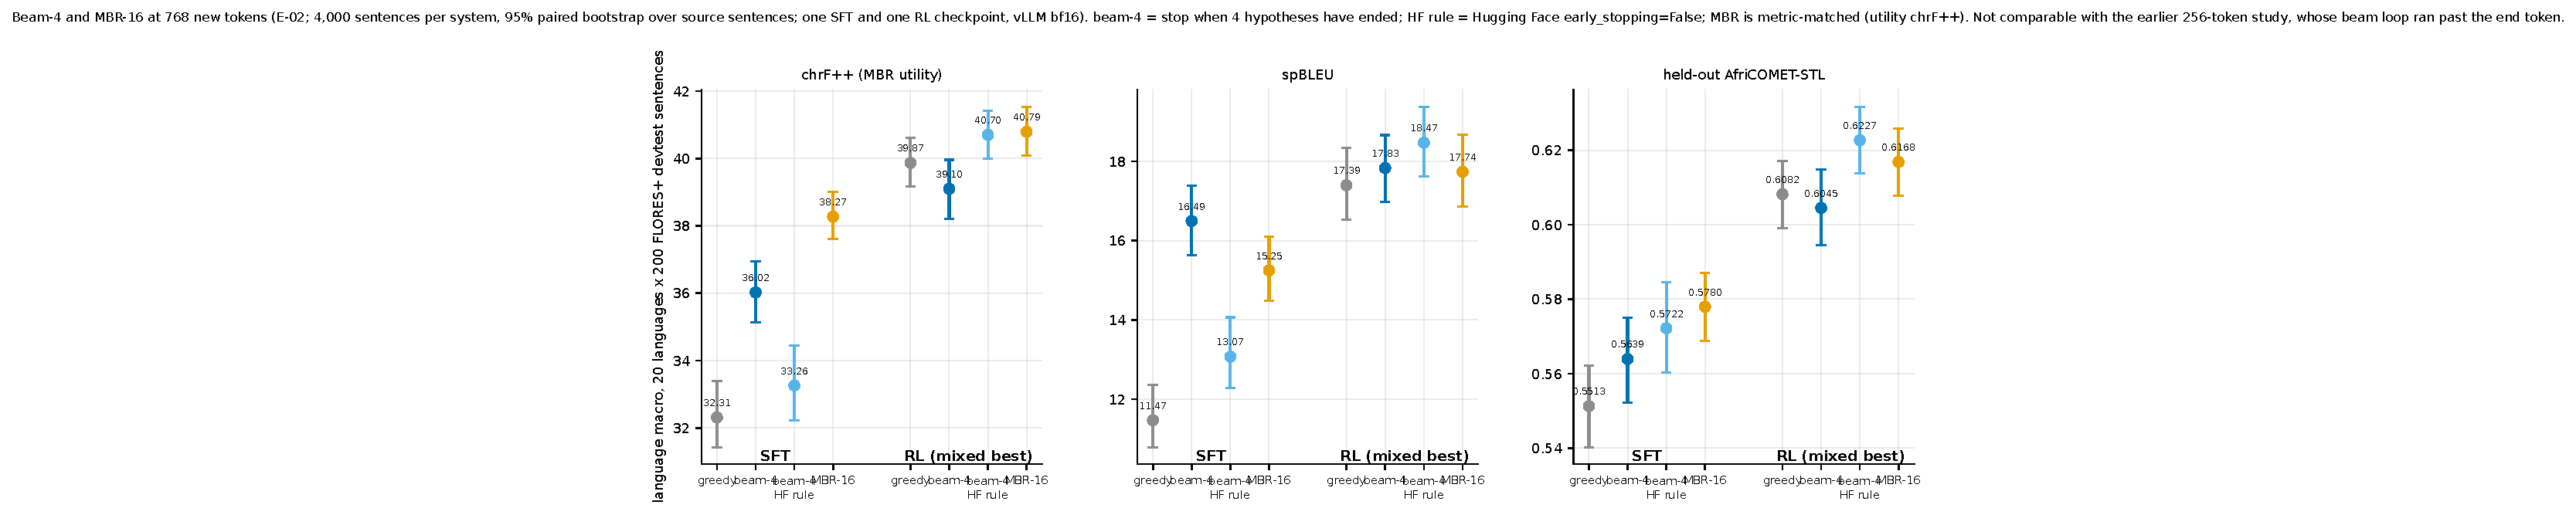
\includegraphics[width=1.00\linewidth,trim=384bp 0 384bp 26bp,clip]{figures/fig15_e02_decoding.pdf}
\caption{Greedy, beam-4 and MBR-16 at 768 new tokens (E-02) for the SFT and the RL model (mixed best): chrF++, spBLEU and held-out AfriCOMET-STL, language macro over 20 languages $\times$ 200 FLORES+ devtest sentences (4,000 per system), 95\% paired bootstrap over source sentences; beam-4 stops when 4 hypotheses have ended, the HF rule is early\_stopping=False, MBR is metric-matched (utility chrF++). One SFT and one RL checkpoint, vLLM bf16. Not comparable with the earlier 256-token study. Source: \texttt{reports/\allowbreak{}data/\allowbreak{}e02\_\allowbreak{}beam\_\allowbreak{}mbr\_\allowbreak{}768\_\allowbreak{}2026-\allowbreak{}11-\allowbreak{}05/\allowbreak{}cmp\_\allowbreak{}all.\allowbreak{}json}.}\label{fig:decoding_app}
\end{figure}

\begin{figure}[t]
\centering
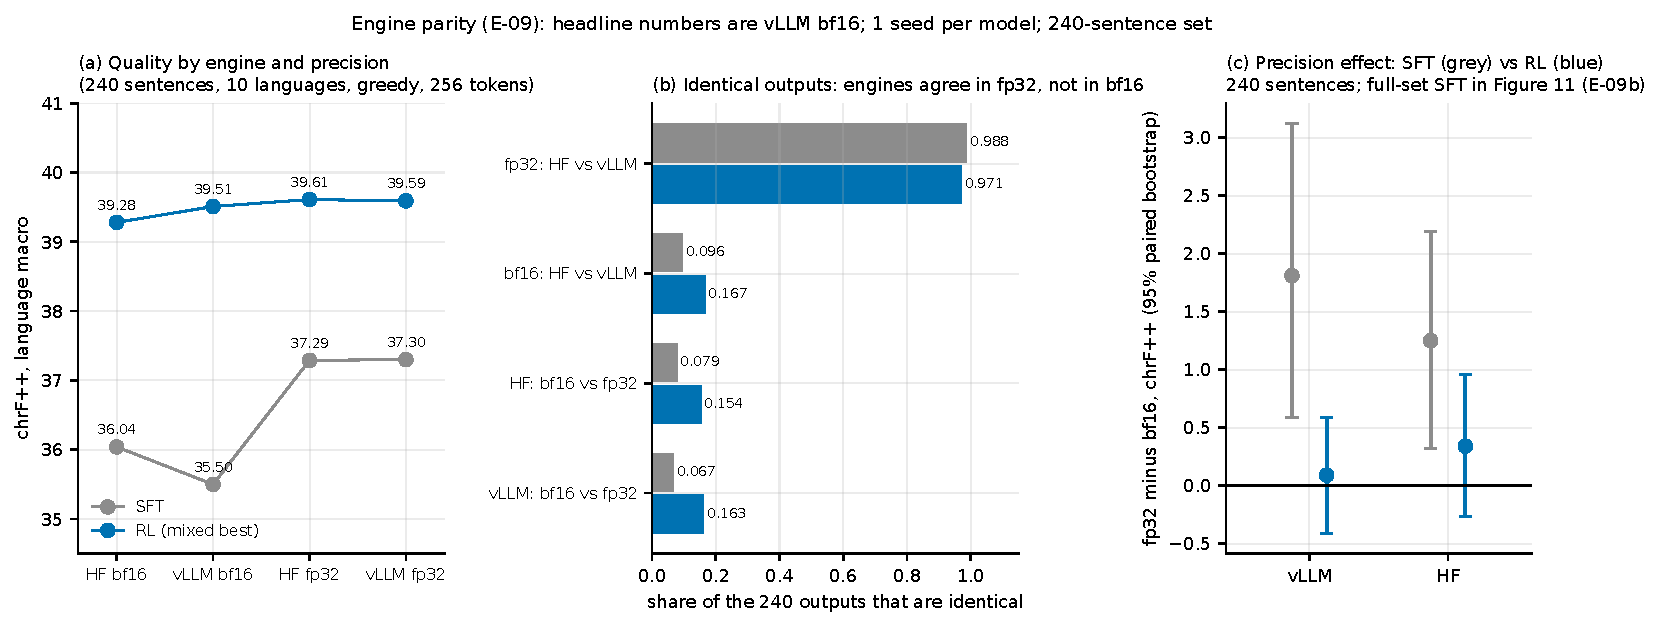
\includegraphics[width=1.00\linewidth]{figures/fig8_engine_parity.pdf}
\caption{Engine parity (E-09), 240 sentences (10 languages $\times$ 24 FLORES+ devtest sentences), greedy, 256 new tokens, SFT and RL (mixed best), one seed. (a) Language-macro chrF++ by engine and precision. (b) Share of identical outputs: vLLM and HF agree in fp32 (0.988, 0.971) and not in bf16 (0.096, 0.167). (c) fp32 minus bf16 chrF++ with 95\% paired bootstrap over sentences: negligible for the RL model, +1.81 [+0.59, +3.12] (vLLM) for the SFT on this small set, which the full-set run of Figure 11 does not reproduce. Headline numbers of the paper are vLLM bf16. Sources: \texttt{reports/\allowbreak{}data/\allowbreak{}e09\_\allowbreak{}engine\_\allowbreak{}parity\_\allowbreak{}2026-\allowbreak{}11-\allowbreak{}04/\allowbreak{}\{parity\_\allowbreak{}bootstrap,parity\_\allowbreak{}summary\}.\allowbreak{}json}.}\label{fig:fig8_engine_parity}
\end{figure}

\begin{figure}[t]
\centering
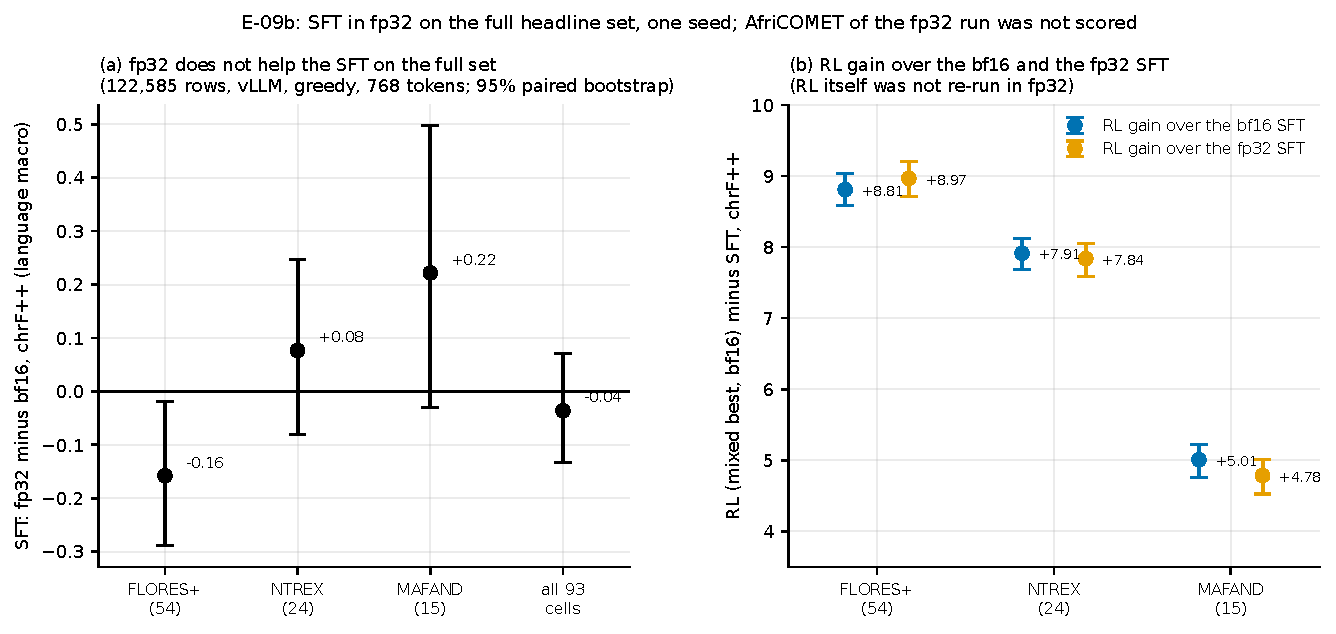
\includegraphics[width=0.90\linewidth]{figures/fig11_fp32_full_set.pdf}
\caption{Full-set precision check (E-09b): the SFT generated in fp32 instead of bf16 (vLLM, greedy, 768 new tokens, 122,585 rows, 214 flagged rows removed; one seed). (a) fp32 minus bf16 chrF++ (language macro, 95\% paired bootstrap over sentences) on FLORES+ (54 languages), NTREX (24), MAFAND (15) and over all 93 cells (\ensuremath{-}0.04 [\ensuremath{-}0.13, +0.07]). (b) RL gain (mixed best, bf16) over the bf16 SFT and over the fp32 SFT. The RL model was not re-run in fp32 and the AfriCOMET of the fp32 run was not scored. Source: \texttt{reports/\allowbreak{}data/\allowbreak{}e09b\_\allowbreak{}fp32\_\allowbreak{}2026-\allowbreak{}11-\allowbreak{}04/\allowbreak{}evidence\_\allowbreak{}e09b.\allowbreak{}json}.}\label{fig:fig11_fp32_full_set}
\end{figure}

\section{NLLB comparison and other systems: details}\label{app:afrique}

The RL closes 74\% of the gap between the SFT and NLLB-3.3B (12.50 $\to$ 3.26; arithmetic of the two differences), and stage A alone gives 8.61 of the 9.24 chrF++ that the mixed best adds over the SFT on these languages (93\%). The remaining gap is not a finishing or looping artefact: on these 43 languages the mixed best finishes at least 0.99 and repeats at most 0.02 in every language. By NLLB-3.3B tertile (14 / 14 / 15 languages) the mixed best reaches 91.7\% (high, 46.82 against 51.05), 87.7\% (mid, 34.57 against 39.42) and 96.8\% (tail, 25.92 against 26.78) of NLLB-3.3B; the SFT 75.3\%, 63.2\% and 60.7\%. The mixed best matches or beats NLLB-3.3B on 7 of 43 languages, all in the lowest tertile (yor +5.43, fon +2.95, dyu +2.77, wol +2.48, kam +2.32, kmb +2.22, umb +1.86; the SFT only on fon, 20.17 against 19.30) and is within 1 chrF++ on 9. The largest remaining gaps are amh \ensuremath{-}11.28, kin \ensuremath{-}9.74, kea \ensuremath{-}8.72, run \ensuremath{-}8.02, ewe \ensuremath{-}7.03, lug \ensuremath{-}6.77, tir \ensuremath{-}6.06 and hau \ensuremath{-}6.04. 
% src: NLLBRL sections 0, 2, 3 (`table3_by_nllb_tertile.csv`, `table2_per_language_43.csv`)

\textbf{Same sentences.} In the post-editor run, NLLB-3.3B and RL stage A drafts were scored on identical 100-sentence FLORES+ subsets (language bootstrap only; sentence hypotheses are not stored). With beam-4 on our side (the beam setup of the post-editor run, not that of E-02) and NLLB greedy on theirs, stage A is 1.44 below NLLB-3.3B on 43 languages (36.12 against 37.56, [\ensuremath{-}2.34, \ensuremath{-}0.56]; 13 languages at least equal) and 3.67 below on all 50 languages both have; held-out AfriCOMET 0.6414 against 0.6709 (\ensuremath{-}0.0294 [\ensuremath{-}0.0366, \ensuremath{-}0.0222], 40 languages, ahead in 5). Our own NLLB run on 100 sentences is 1.23 [\ensuremath{-}1.60, \ensuremath{-}0.86] below the published full-devtest value, which bounds the sample and reference effects. AfriCOMET is the QE reward's family, so that row is not independent evidence for the RL model. 
% src: NLLBRL section 4 (`table6b_same_sentence_summary.csv`, `table7_africomet_same_100_sentences.csv`)

\textbf{AfriqueLLM family, indicative only.} On the 21 languages with per-language values in the 5-shot AfroBench-Lite harness (afr amh ewe hau ibo kin lin lug nya orm sna som sot swh tir tsn twi wol xho yor zul): SFT 32.37, stage A 39.13, B1 best 39.32, mixed best 39.40, weak final 39.26, against AfriqueQwen3.5-4B-50Langs 41.71 (mixed best \ensuremath{-}2.31; ahead in 4 of 21 languages), AfriqueGemma-12B 38.58 (+0.83; 6 of 21), AfriqueLlama-8B 36.71, AfriqueQwen-14B 36.67, AfriqueQwen-8B 35.06, AfriqueGemma-4B 31.12, Gemma3-12B 18.82, Llama3.1-8B 16.45. Those are base models in 5-shot prompting with a harness whose chrF++ implementation and FLORES split are not verified.   Bidirectional aggregates (TranslatePsy, AfriNLLB) and pooled AfroBench rows are not comparable and are not compared.
% src: NLLBRL section 5 `table5_afrique_21_languages.csv`; ledger N3 status weak

\section{Family, script and resource level (exploratory, fragile)}\label{app:family}

We labelled all 125 registry languages with Glottolog 5.3 \citep{glottolog53} (CLDF release v5.3, commit 072ca0d of glottolog-cldf, CC BY 4.0, Zenodo 10.5281/zenodo.18840967) and asked whether the RL gain (mixed best minus SFT, FLORES+ devtest chrF++, 54 languages) depends on family, script or resource level. \textbf{This analysis is observational, has 54 languages in 7 families, several with 1 to 3 members, and its main result changes with the languages included. We report it as description, not as a finding.} 
% src: FAMILY sections 0, 3-5

\begin{table}[t]
\centering\scriptsize
\setlength{\tabcolsep}{4pt}
\caption{RL gain (mixed best minus SFT, FLORES+ devtest \chrfpp{}, 54 languages) by Glottolog family, script and regression family; bootstrap over languages.}\label{tab:family}
\begin{tabularx}{\linewidth}{@{}l>{\raggedright\arraybackslash}Xrr>{\raggedright\arraybackslash}X@{}}
\toprule
grouping & group & n & mean SFT chrF++ & mean gain [bootstrap CI over languages] \\
\midrule
Glottolog top family & Atlantic-Congo & 33 & 26.20 & +9.14 [+7.58, +10.79] \\
 & Afro-Asiatic & 11 & 13.45 & +6.89 [+4.29, +9.89] \\
 & Nilotic & 3 & 12.87 & +11.58 [+10.30, +13.13] \\
 & Indo-European (creoles, Afrikaans) & 3 & 36.85 & +10.23 [+1.01, +20.27] \\
 & Mande & 2 & 14.65 & +8.42 [+7.78, +9.06] \\
regression family & Narrow Bantu & 24 & 27.36 & +9.91 [+7.96, +11.71] \\
 & other Atlantic-Congo & 9 & 23.11 & +7.06 [+4.76, +9.61] \\
script & Latin & 48 & 24.84 & +9.32 [+8.03, +10.68] \\
 & Ethiopic (amh tir) & 2 & 13.55 & +9.13 [+8.26, +10.00] \\
 & Arabic (aeb ary arz) & 3 & 4.00 & +2.73 [+1.36, +4.59] \\
 & Tifinagh (zgh) & 1 & 2.29 & +1.78 \\
\bottomrule
\end{tabularx}
\end{table}

(Single-language groups, Saharan knc and Austronesian mlg, are in the report. Glottolog's Nilotic group differs from the earlier ``Nilo-Saharan'' group of EVID Table 4 by dik versus knc, which is why the two means agree, +11.58 and +11.62.)

\begin{itemize}
\item The lowest gains are the Arabic-script dialects and Tifinagh, the languages where the SFT's output was English, Arabic or loops and the RL did not repair it (Section~\ref{sec:rlsft}). The eight languages that lacked a family label are now labelled: aeb, ary and arz Afro-Asiatic (Semitic, Arabic script), taq and zgh Afro-Asiatic (Berber), cjk Narrow Bantu, dik Nilotic, mfe French-lexifier creole. 
% src: FAMILY section 2 (`unlabelled8_labels.csv`)
\item \textbf{The gain is not explained by the token budget} (Spearman rho(gain, log10 SFT tokens) = \ensuremath{-}0.16 [\ensuremath{-}0.44, +0.13], n = 54; OLS slope +0.34 chrF++ per log10 unit [\ensuremath{-}2.03, +1.79], R2 0.003), while the SFT level is (rho = +0.68 [+0.47, +0.82]; slope +11.8 [+8.5, +17.0], R2 0.45). \textbf{This is fragile:} dropping Afro-Asiatic turns the slope on the gain from +0.34 into \ensuremath{-}3.00 (SE 1.06), so ``no relation'' depends on which languages are in the sample. What the gain does track is the SFT's failure rate (rho with the SFT finished rate \ensuremath{-}0.47 [\ensuremath{-}0.74, \ensuremath{-}0.15], with its repeat rate +0.46 [+0.13, +0.72], n = 54 each), in line with Section~\ref{sec:rlsft}: family, script and resource effects on the raw gain are largely effects on how badly the SFT failed.
\item A regression of the gain on family, log tokens, non-Latin script, AfriCOMET availability and NLLB-mined share (n = 53, 11 parameters) explains little (R2 0.27, adjusted 0.09). Only non-Bantu against Narrow Bantu Atlantic-Congo is clearly non-zero (\ensuremath{-}4.45 [\ensuremath{-}8.36, \ensuremath{-}1.24], robust p = 0.020, uncorrected for the many contrasts); the NLLB-mined share is positive (+7.57 [+0.91, +14.67], p = 0.066), which reflects that NLLB-dependent languages are the low-resource tail that started low and failed by loops; it does not say whether NLLB data helped or hurt (Appendix~\ref{app:nllblink}). The same model explains most of the SFT level (R2 0.67, adjusted 0.59). Family, script, tokens, resource tier and AfriCOMET availability overlap (VIF 2.1 to 3.4), and three of six mixed-model fits did not converge.
\item Only 54 of 125 languages (58 with NTREX and MAFAND) have a gain; 51 have no reference test, so no family or script statement is possible for them. The 54 are the better-resourced languages (median 25.4 M tokens against 8.6 M for the Latin-script registry). The token table is provisional, the script of 51 languages is assigned from prior knowledge, and the analysis was run after the results were known.
\end{itemize}

\section{Science and document results: details}\label{app:docs}

Start: the mixed-stage best. Science SFT: AdamW 3e-6, 283 steps of 65,536 tokens (6.34 M AfriScience tokens in 6 languages, two passes, plus 12.19 M replay tokens), AfriScience dev loss 1.699 $\to$ 1.322. The SFT end point (alpha 1.0) loses 2.45 NTREX and 1.20 MAFAND chrF++, so the weights were interpolated, theta(alpha) = (1 - alpha) theta\_start + alpha theta\_science, with a rule fixed beforehand (best AfriScience dev chrF subject to NTREX and MAFAND not more than 0.5 below the start); alpha = 0.5 was chosen. 
% src: reports/eval_science_sft_385m_2026-11-04.md

\begin{table}[t]
\centering\footnotesize
\setlength{\tabcolsep}{4pt}
\caption{Weight interpolation sweep of the science SFT, AfriScience-MT test (macro over six languages), with NTREX and MAFAND-MT \chrfpp{} (last two columns). SSA-QE = SSA-COMET-QE (headline); AfriC. = AfriCOMET-STL.}\label{tab:alpha}
\begin{tabular}{@{}rrrrrrrrr@{}}
\toprule
$\alpha$ & SSA-QE & chrF & chrF++ & BLEU & spBLEU & AfriC. & NTREX & MAFAND \\
\midrule
0 & 0.6130 & 45.40 & 42.44 & 17.72 & 21.89 & 0.6828 & 37.16 & 40.78 \\
0.3 & 0.6128 & 46.28 & 43.40 & 18.73 & 23.25 & 0.6865 & 37.13 & 41.06 \\
0.5 (chosen) & 0.6118 & 46.63 & 43.80 & 19.27 & 23.87 & 0.6879 & 36.90 & 41.05 \\
0.7 & 0.6092 & 46.56 & 43.81 & 18.98 & 23.83 & 0.6859 & 36.43 & 40.83 \\
1.0 & 0.5986 & 44.92 & 42.30 & 16.78 & 20.87 & 0.6708 & 34.71 & 39.58 \\
\bottomrule
\end{tabular}
\end{table}

\textbf{The science SFT gives surface gains (chrF +1.2, BLEU +1.5, spBLEU +2.0 at alpha 0.5) and no SSA-COMET-QE gain} (dev 0.6242 against 0.6235). SSA-COMET-QE here is the reference-free \texttt{McGill-\allowbreak{}NLP/\allowbreak{}ssa-\allowbreak{}comet-\allowbreak{}qe}, the variant that reproduces the AfriScience-MT paper's released values (mean absolute difference 0.006 over the six strongest released runs, 0.031 over nine); there is no RL in this comparison, so it is independent of the reward.  The metric choice was made after the alpha rule (Appendix~\ref{app:disc}). The 385M with the science SFT is below the old 270M science-stage models on AfriScience test chrF (46.6 against 47.9 for the old RL-final, 50.0 and 50.2 for the old science-stage models) and below the published fine-tuned NLLB-1.3B (52.3). 
% src: SCI alpha sweep; DOC calibration; HYG X13 (SCI's caveat paragraph is stale, quote DOC)
% src: SCI Table 2

\textbf{Science RL.} The run executed 160 steps (cap extended from 150 to 190 at step 120, stopped on a dev plateau at step 150 plus a 10-step wind-down; Appendix~\ref{app:chain}, ledger X24). Evaluation was fixed in advance: independent evidence = plain chrF on AfriScience-MT test and held-out AfriCOMET; SSA-COMET-QE and SSA-COMET-MTL are reward-family and shown but not counted. The final checkpoint is a small real sentence-level gain over its start (science SFT, alpha 0.5): chrF +0.46 [+0.27, +0.65] on AfriScience test and held-out AfriCOMET +0.0053 [+0.0036, +0.0071]; the step-75 \texttt{best} checkpoint is smaller (chrF +0.16 [\ensuremath{-}0.04, +0.37]); SSA-COMET-QE moves by +0.004 only; NTREX and MAFAND do not regress (chrF++ +0.42, +0.10). There is no document-level gain: chunked window SSA-COMET-QE is 0.574 (start), 0.574 (best), 0.577 (final), and the earlier 270M work's 270M models stay ahead on sentence chrF (47.9-50.2 stored numbers against 47.10) and on chunked documents (0.593 against 0.577). One run, one seed. Numbers: \texttt{reports/\allowbreak{}eval\_\allowbreak{}science\_\allowbreak{}rl\_\allowbreak{}385m\_\allowbreak{}2026-\allowbreak{}11-\allowbreak{}04.\allowbreak{}md}. \textbf{Disclosure:} the long-document RL start model was changed from \texttt{best} to \texttt{final} after this evaluation, including its test numbers (rule refined on the full AfriScience dev set, where final beats best by +0.24 chrF and +0.0031 AfriCOMET; the test split was not used for the rule); logged in \texttt{reports/\allowbreak{}overnight\_\allowbreak{}log\_\allowbreak{}2026-\allowbreak{}11-\allowbreak{}04.\allowbreak{}md}. SSA-COMET-QE, AfriCOMET and chrF for every stage are tabulated below (E-05). The RL-only science arm (mixed best to science RL without the science SFT) is reported next (E-14).

\textbf{Science RL without the science SFT (E-14).} To ask whether the science SFT is needed, the executed science RL was repeated with the start model changed to the mixed best (= science-SFT alpha 0, the model the science SFT was built from): same seed 1234, same pool, same reward, Muon at 1e-6, KL 0.1 against the start model, 160 steps (150 plus a 10-step wind-down), pre-declared checkpoint = final. The rule was registered before the run: the science SFT is \emph{not needed} if the lower 95\% bounds of E-14 minus the science RL final on AfriScience-MT test are above \ensuremath{-}0.5 chrF and above \ensuremath{-}0.004 held-out AfriCOMET; it is \emph{needed} if the upper bound of either is below its margin. 

\begin{table}[t]
\centering\footnotesize
\setlength{\tabcolsep}{4pt}
\caption{Science RL without the science SFT (E-14): AfriScience-MT test, sentence level, macro over 6 languages.}\label{tab:e14a}
\begin{tabularx}{\linewidth}{@{}>{\raggedright\arraybackslash}Xrrrr@{}}
\toprule
model & chrF & chrF++ & AfriCOMET-STL (held out) & SSA-COMET-QE (reward family) \\
\midrule
mixed best (= alpha 0; E-14's start) & 45.40 & 42.44 & 0.6828 & 0.6130 \\
B1 final (stage-B1 RL) & 45.45 & 42.50 & 0.6846 & 0.6141 \\
\textbf{E-14 final (science RL, no science SFT)} & \textbf{45.66} & 42.69 & \textbf{0.6850} & 0.6153 \\
science SFT alpha 0.5 & 46.63 & 43.80 & 0.6879 & 0.6118 \\
science RL final (from the science SFT) & 47.10 & 44.22 & 0.6932 & 0.6158 \\
\bottomrule
\end{tabularx}
\end{table}

\begin{table}[t]
\centering\footnotesize
\setlength{\tabcolsep}{4pt}
\caption{E-14 final minus X, 95\% bootstrap (independent weights per language).}\label{tab:e14b}
\begin{tabularx}{\linewidth}{@{}>{\raggedright\arraybackslash}Xll>{\raggedright\arraybackslash}X@{}}
\toprule
E-14 final minus & chrF & AfriCOMET-STL (held out) & SSA-COMET-QE (reward family) \\
\midrule
science RL final (from the science SFT) & \textbf{-1.44 [\ensuremath{-}1.61, \ensuremath{-}1.25]} & \textbf{-0.0082 [\ensuremath{-}0.0101, \ensuremath{-}0.0065]} & \ensuremath{-}0.0006 [\ensuremath{-}0.0018, +0.0007] \\
science SFT alpha 0.5 & \ensuremath{-}0.97 [\ensuremath{-}1.20, \ensuremath{-}0.75] & \ensuremath{-}0.0030 [\ensuremath{-}0.0050, \ensuremath{-}0.0009] & +0.0035 [+0.0022, +0.0047] \\
mixed best (its own start) & +0.26 [+0.12, +0.39] & +0.0022 [+0.0007, +0.0036] & +0.0023 [+0.0013, +0.0033] \\
B1 final & +0.21 [+0.07, +0.36] & +0.0004 [\ensuremath{-}0.0012, +0.0020] & +0.0012 [+0.0000, +0.0023] \\
\bottomrule
\end{tabularx}
\end{table}

\textbf{By the registered rule the science SFT is needed:} the upper bounds are \ensuremath{-}1.25 chrF and \ensuremath{-}0.0065 AfriCOMET, both below their margins, chrF is lower in all six languages (\ensuremath{-}0.72 to \ensuremath{-}2.70) and the dev split agrees (\ensuremath{-}1.63 [\ensuremath{-}1.81, \ensuremath{-}1.44]). The science gain is carried by the science SFT (+1.23 chrF at alpha 0.5), not by the science RL: the RL alone on top of the mixed best adds +0.26 chrF [+0.12, +0.39] (+0.0022 AfriCOMET), a gain of the size at which seed noise matters (E-04), against +0.46 for the RL on top of the science SFT. The trainer's dev chrF++ stayed flat (43.50 $\to$ 43.43) while the executed science RL rose from 44.62 to 45.13, and no \texttt{best/\allowbreak{}} checkpoint was written (the dev macro never rose by the trainer's 0.2 margin), so only the final exists. \textbf{Reward-family caveat:} SSA-COMET-QE rates E-14 level with the science RL final (\ensuremath{-}0.0006 [\ensuremath{-}0.0018, +0.0007]) and above alpha 0.5 (+0.0035), while chrF and held-out AfriCOMET rate it below both: the metric the RL optimises moved without a matching move in the independent metrics, so it is not evidence of quality here. On the general benchmarks (93 cells) E-14 is +0.13 chrF++ [+0.10, +0.15] over the mixed best (FLORES+ +0.17, NTREX +0.12, MAFAND 0.00) and +0.34 [+0.31, +0.36] over B1 final, with no regression on NTREX and MAFAND (+0.12 / 0.00 against the mixed best; the executed science RL final is higher on MAFAND by 0.36); at document level it does not change chunked chrF (57.30 against 57.29 for its start) and whole-document decoding still fails (finished 0.69, loop 0.82, chrF 25.6). Caveats: one seed; one crash (a CUDA out-of-memory in the COMET reward worker at about step 38; the launcher's ladder halved the micro-batch from 12,288 to 6,144 tokens and resumed from the step-20 checkpoint, replaying steps 21 to 38, which can differ from the first pass because vLLM sampling is not bit-reproducible); the comparison with the science RL final mixes the effect of the science SFT with its alpha 0.5 interpolation (a science SFT at alpha 1.0 followed by RL was not run); 160 steps only. 
% src: reports/e14_science_rl_without_science_sft_2026-11-05.md sections 0-3; reports/data/e14_science_rl_no_sft_2026-11-05/ (ledger E14 rows SC7, SC8)

\textbf{SSA-COMET-QE for every stage (E-05).} The stored AfriScience-MT sentence predictions of every stage were scored with \texttt{McGill-\allowbreak{}NLP/\allowbreak{}ssa-\allowbreak{}comet-\allowbreak{}qe}, held-out AfriCOMET-STL and plain chrF (test, macro over 6 languages). SSA-COMET-QE is 0.5686 for the SFT and 0.6118 (stage A), 0.6113 (B1 best), 0.6130 (mixed best), 0.6118 (science SFT alpha 0.5), 0.6135 / 0.6158 (science RL best / final) and 0.6158 / 0.6165 (long-document RL best / final) for the RL stages: the first RL stage adds +0.043 and every later stage at most +0.005 more. It is a reward-family metric for every RL row, so these numbers are not evidence of quality; chrF (36.00 for the SFT, 45.06 stage A, 45.40 mixed, 46.63 science SFT, 47.10 science RL final, 47.16 long-document RL) and held-out AfriCOMET-STL (0.6064, 0.6822, 0.6828, 0.6879, 0.6932, 0.6936) keep rising by small steps that SSA-COMET-QE does not register. Alpha 1.0 (the full science SFT) is the only row clearly worse (0.5986). One seed per stage; test-sentence bootstrap intervals of the differences are +/\ensuremath{-}0.001 to +/\ensuremath{-}0.002 (Section~\ref{sec:science} tables). The numbers are for sentence level and are not comparable with the AfriScience-MT paper's document-level table. 
% src: reports/e05_ssa_all_stages_2026-11-04.md; reports/data/e05_ssa_all_stages_2026-11-04/{tables.md,e05_all.json} (ledger SC6, P4)

168 test documents (28 papers $\times$ 6 languages), a document being the paper's plain-language summary rebuilt from sentences. Whole-document generation (greedy, 4,096 new tokens) fails for the 385M models and is worse after the science SFT: start finished 0.71, loop 0.86, chrF 22.8, tail coverage 0.27; science SFT finished 0.51, loop 0.86, chrF 24.9; the old 270M RL-final finished 0.70, loop 0.61, chrF 34.9. Sentence-by-sentence (``chunked'') decoding with best-of-4 repair fixes finishing for all three (finished 1.00, sentence coverage 1.000): 
% src: reports/eval_afriscience_document_level_2026-11-04.md Tables 1-3

\begin{table}[t]
\centering\footnotesize
\setlength{\tabcolsep}{4pt}
\caption{Chunked document decoding (sentence by sentence with best-of-4 repair), 168 test documents.}\label{tab:docs}
\begin{tabularx}{\linewidth}{@{}>{\raggedright\arraybackslash}Xrrrr@{}}
\toprule
model (chunked) & SSA-COMET-QE, 4-sentence windows & chrF & AfriCOMET window & BLEU \\
\midrule
385M start (alpha 0) & 0.574 & 57.3 & 0.687 & 20.0 \\
385M science SFT (alpha 0.5) & 0.574 & 58.8 & 0.692 & 22.0 \\
old 270M RL-final (earlier 270M work) & 0.593 & 59.3 & 0.703 & 22.5 \\
\bottomrule
\end{tabularx}
\end{table}

The earlier 270M work's 270M RL-final is as good as or better than the 385M at document level (+0.019 window SSA-COMET-QE, +0.011 AfriCOMET window, +0.5 to +2.0 chrF; better on hau, lug, nso, zul, worse on amh). The COMET encoders read 512 tokens, so a concatenated-document COMET only sees the start of a document; the window values are the honest ones. Window SSA-COMET-QE is reward-family for the old model (trained against a QE reward); chrF and AfriCOMET are the independent checks. For reference, the AfriScience-MT paper's best released document-level system (GPT-5.4) has SSA-COMET 0.519 and chrF 64.5 under document handling we cannot reproduce. Caveats: one seed, 28 papers per language, no bootstrap. None of the 385M RL stages trained on prompts above 256 source tokens before the long-document RL; production use is sentence by sentence.

\textbf{Long-document RL.} The stage started from the science RL final (step 160), ran the planned 80 steps (32 prompts per step, about 51\% long prompts of 512 to 2,048 source tokens, group 8, no guide, hold-out-reward checkpoint selection, LibreTexts-free pool) and was evaluated at its best (step 50) and final (step 80) checkpoints on the same 168 documents. In whole-document mode, best against its start: finished \textbf{0.70 $\to$ 0.82 (+0.125 [+0.046, +0.204])}, loop rate \textbf{0.85 $\to$ 0.73 (\ensuremath{-}0.113 [\ensuremath{-}0.179, \ensuremath{-}0.056])}, chrF \textbf{27.4 $\to$ 30.9 (+3.4 [+1.5, +5.3])}, tail coverage 0.32 $\to$ 0.36 (95\% bootstrap over documents). The final checkpoint is similar (finished 0.85, loop 0.72, chrF 29.7, +2.2 [+0.4, +4.2], length ratio 0.81); best and final do not differ significantly (chrF \ensuremath{-}1.2 [\ensuremath{-}3.0, +0.7]). \textbf{Whole-document decoding remains unusable:} 15 to 18\% of the documents do not finish, 72 to 73\% show a repetition loop, and the output covers 34 to 36\% of the last third of the paper (chunked: 63\%). Chunked and sentence-level results do not change: window SSA-COMET-QE (reward family) 0.577 $\to$ 0.579 and 0.579 (a corpus-level number, no interval; a 0.002 difference is not an effect), chunked chrF 58.7 $\to$ 58.9 / 58.8 (best +0.13 [+0.04, +0.22]); AfriScience test sentences chrF 47.10 $\to$ 47.16 (+0.06 [\ensuremath{-}0.09, +0.20]), held-out AfriCOMET +0.0001 / +0.0004 with intervals around zero; NTREX / MAFAND chrF++ 37.33 / 41.14 $\to$ 37.43 / 41.15 (best). The earlier 270M work's 270M RL-final is still ahead in chunked mode (window SSA-COMET-QE 0.593 against 0.579) and in whole-document chrF (34.9 against 30.9). The effect is real but moderate and of the size of the other late-stage steps; the hold-out loop rate fell by only 2 points over the 80 steps, and the selection reward is the optimised quantity. One seed; 168 documents from 28 papers, so the intervals reflect paper sampling only. 
% src: reports/eval_long_document_rl_385m_2026-11-04.md sections 0-3 (LDOLR); reports/data/eval_long_rl_2026-11-04/{doc_tables.md,doc_pairs.json,sci_pairs_long.json}; ledger DL5, P2. The report says "best/ vs final/ indistinguishable"; wall-clock and crash loop in Section 15

\subsection{Figures for the science and document results}\label{app:figs}

\begin{figure}[t]
\centering
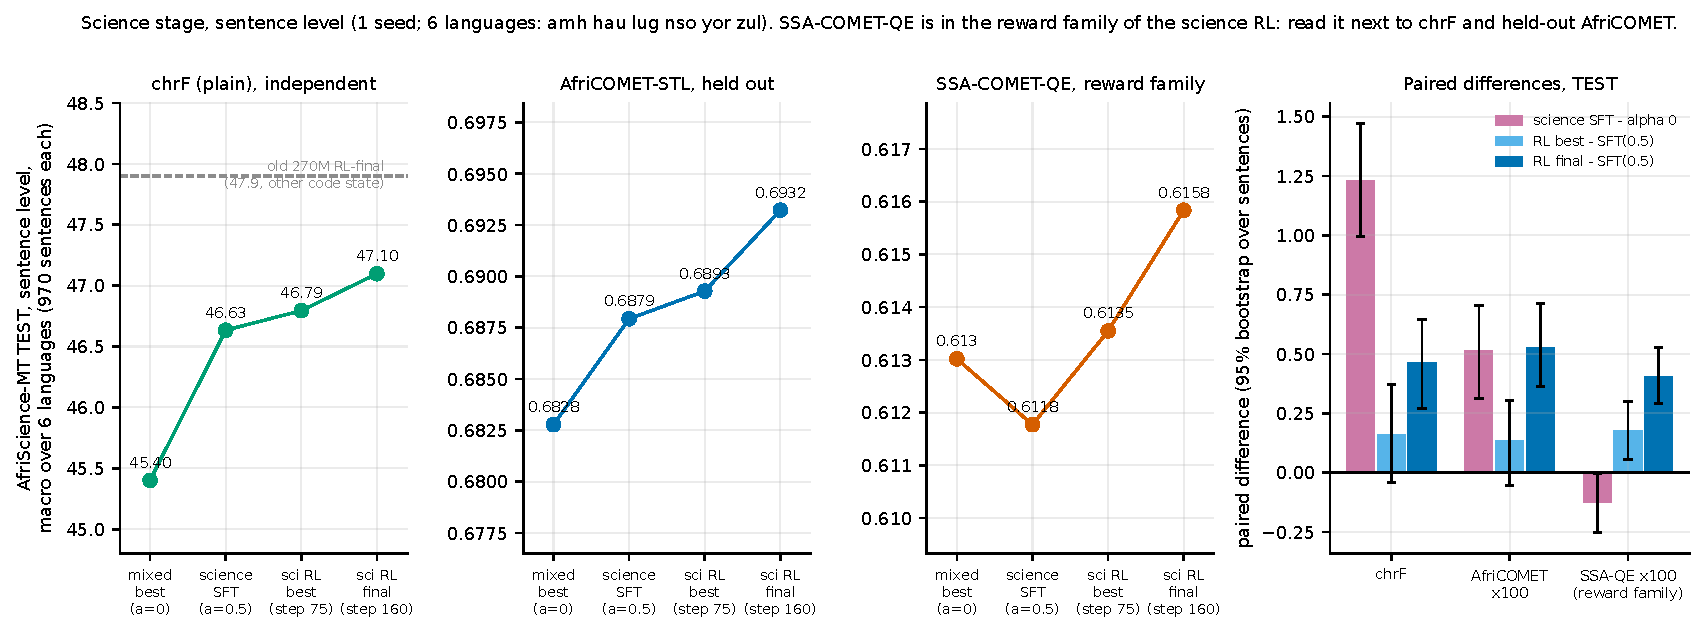
\includegraphics[width=1.00\linewidth]{figures/fig5a_science_sentence.pdf}
\caption{Science stage, AfriScience-MT TEST, sentence level (970 sentences per language, macro over amh hau lug nso yor zul; greedy; one seed): plain chrF (independent of the reward; dashed: the earlier 270M work's 270M RL-final, other code state), held-out AfriCOMET-STL (independent), and SSA-COMET-QE (reward family of the science RL) for the mixed best (alpha 0), the science SFT (alpha 0.5), and the science RL best (step 75) and final (step 160); right: paired differences with 95\% bootstrap over sentences. Sources: \texttt{reports/\allowbreak{}data/\allowbreak{}eval\_\allowbreak{}science\_\allowbreak{}rl\_\allowbreak{}2026-\allowbreak{}11-\allowbreak{}04/\allowbreak{}sci\_\allowbreak{}pairs.\allowbreak{}json}, \texttt{reports/\allowbreak{}data/\allowbreak{}eval\_\allowbreak{}science\_\allowbreak{}sft\_\allowbreak{}2026-\allowbreak{}11-\allowbreak{}04/\allowbreak{}tables.\allowbreak{}md}.}\label{fig:fig5a_science_sentence}
\end{figure}

\begin{figure}[t]
\centering
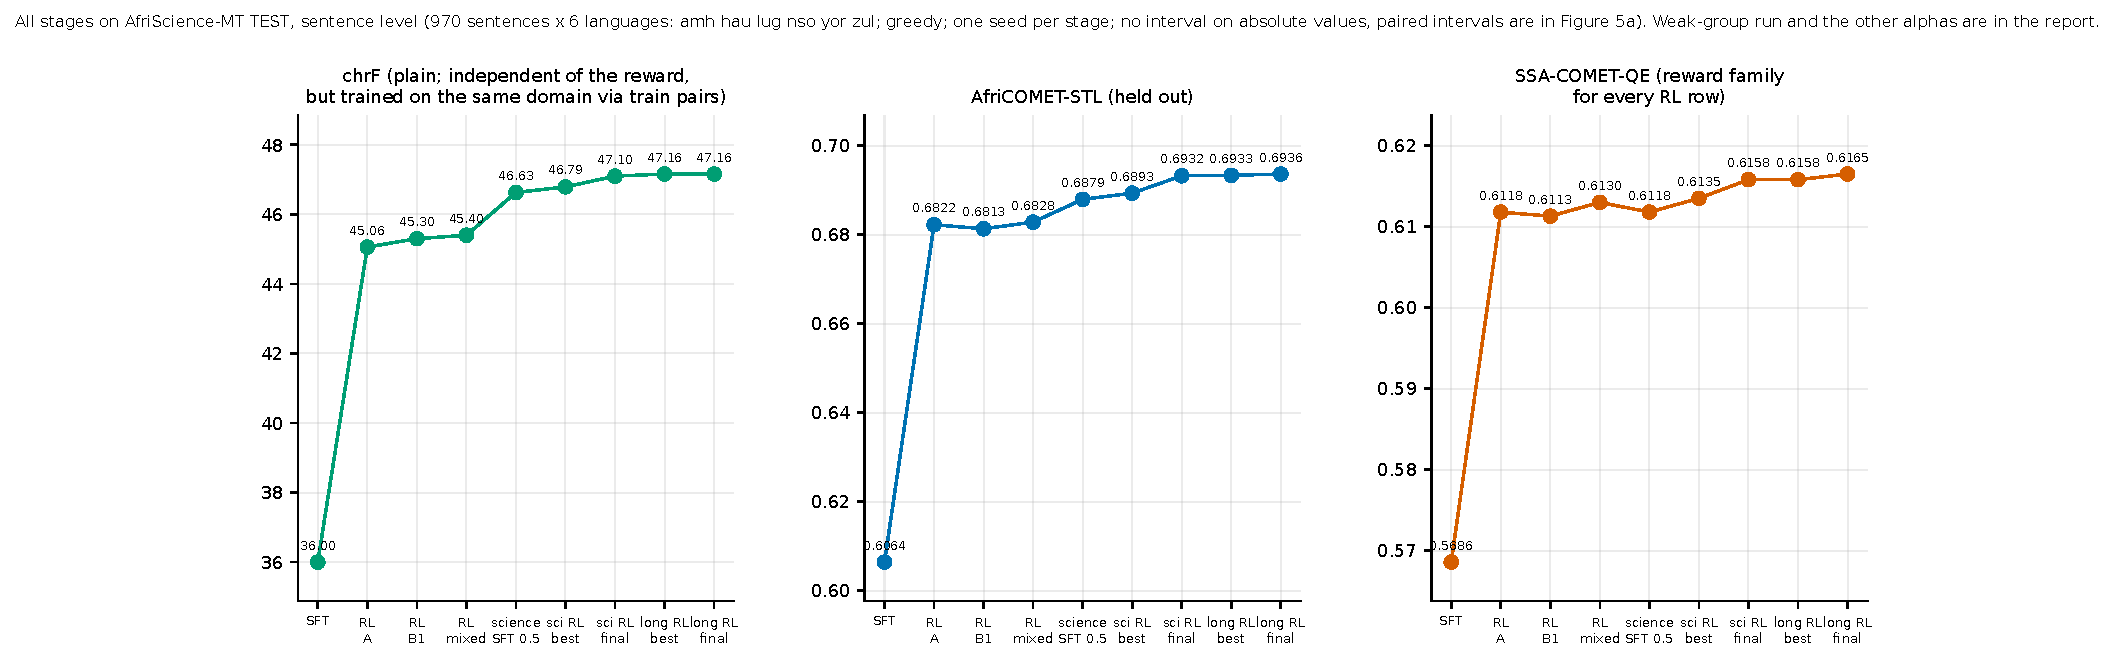
\includegraphics[width=1.00\linewidth]{figures/fig12_ssa_all_stages.pdf}
\caption{All stages on AfriScience-MT TEST, sentence level (970 sentences per language, macro over amh hau lug nso yor zul; greedy; one seed per stage): plain chrF, held-out AfriCOMET-STL and SSA-COMET-QE (reward family for every RL row) for the SFT, RL stages A, B1 and mixed, the science SFT (alpha 0.5), the science RL and the long-document RL. The weak-group run and the other interpolation weights are in the source table. Source: \texttt{reports/\allowbreak{}data/\allowbreak{}e05\_\allowbreak{}ssa\_\allowbreak{}all\_\allowbreak{}stages\_\allowbreak{}2026-\allowbreak{}11-\allowbreak{}04/\allowbreak{}tables.\allowbreak{}md}.}\label{fig:fig12_ssa_all_stages}
\end{figure}

\begin{figure}[t]
\centering
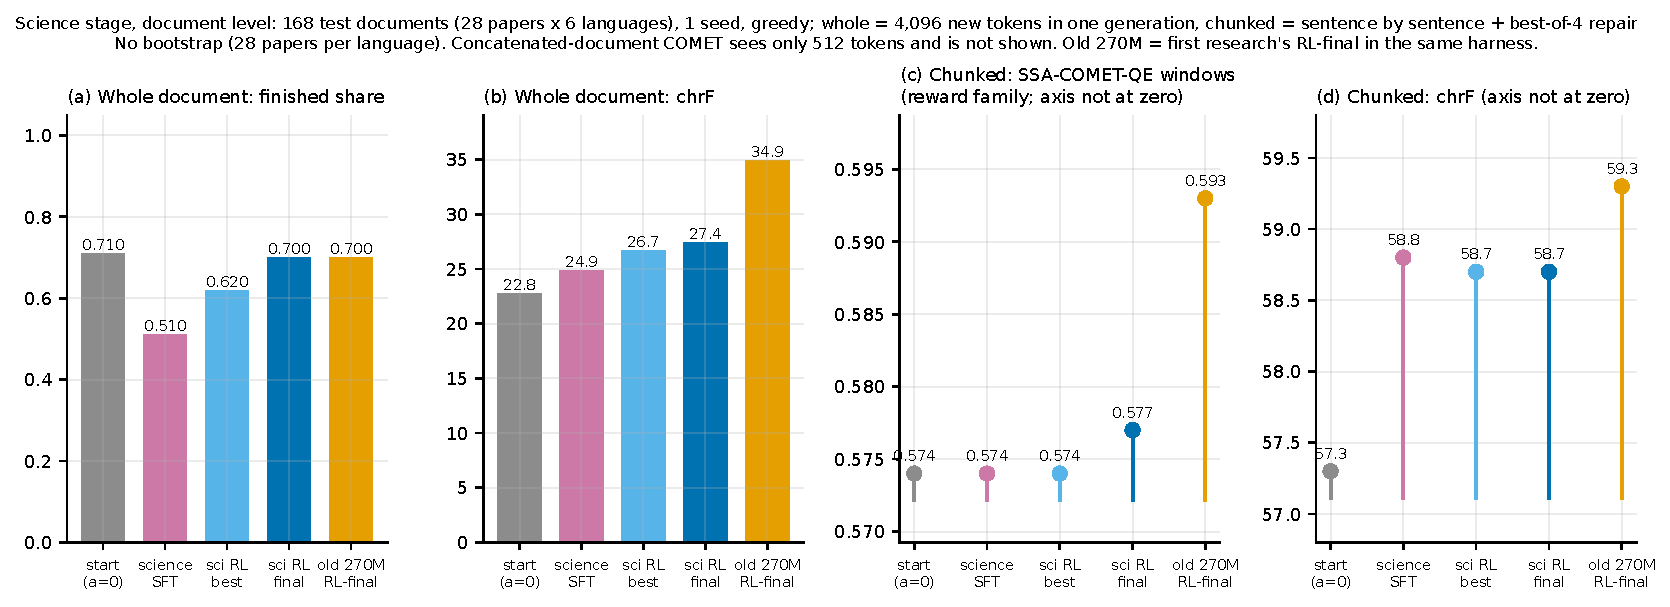
\includegraphics[width=1.00\linewidth]{figures/fig5b_science_document.pdf}
\caption{Science stage, document level: 168 test documents (28 papers $\times$ 6 languages), greedy, one seed, no bootstrap. Whole-document generation (4,096 new tokens): finished share and chrF. Chunked decoding (sentence by sentence plus best-of-4 repair): SSA-COMET-QE on 4-sentence windows (reward family) and chrF; axes of (c) and (d) do not start at zero. Source: \texttt{reports/\allowbreak{}data/\allowbreak{}eval\_\allowbreak{}science\_\allowbreak{}rl\_\allowbreak{}2026-\allowbreak{}11-\allowbreak{}04/\allowbreak{}doc\_\allowbreak{}tables.\allowbreak{}md}.}\label{fig:fig5b_science_document}
\end{figure}

\begin{figure}[t]
\centering
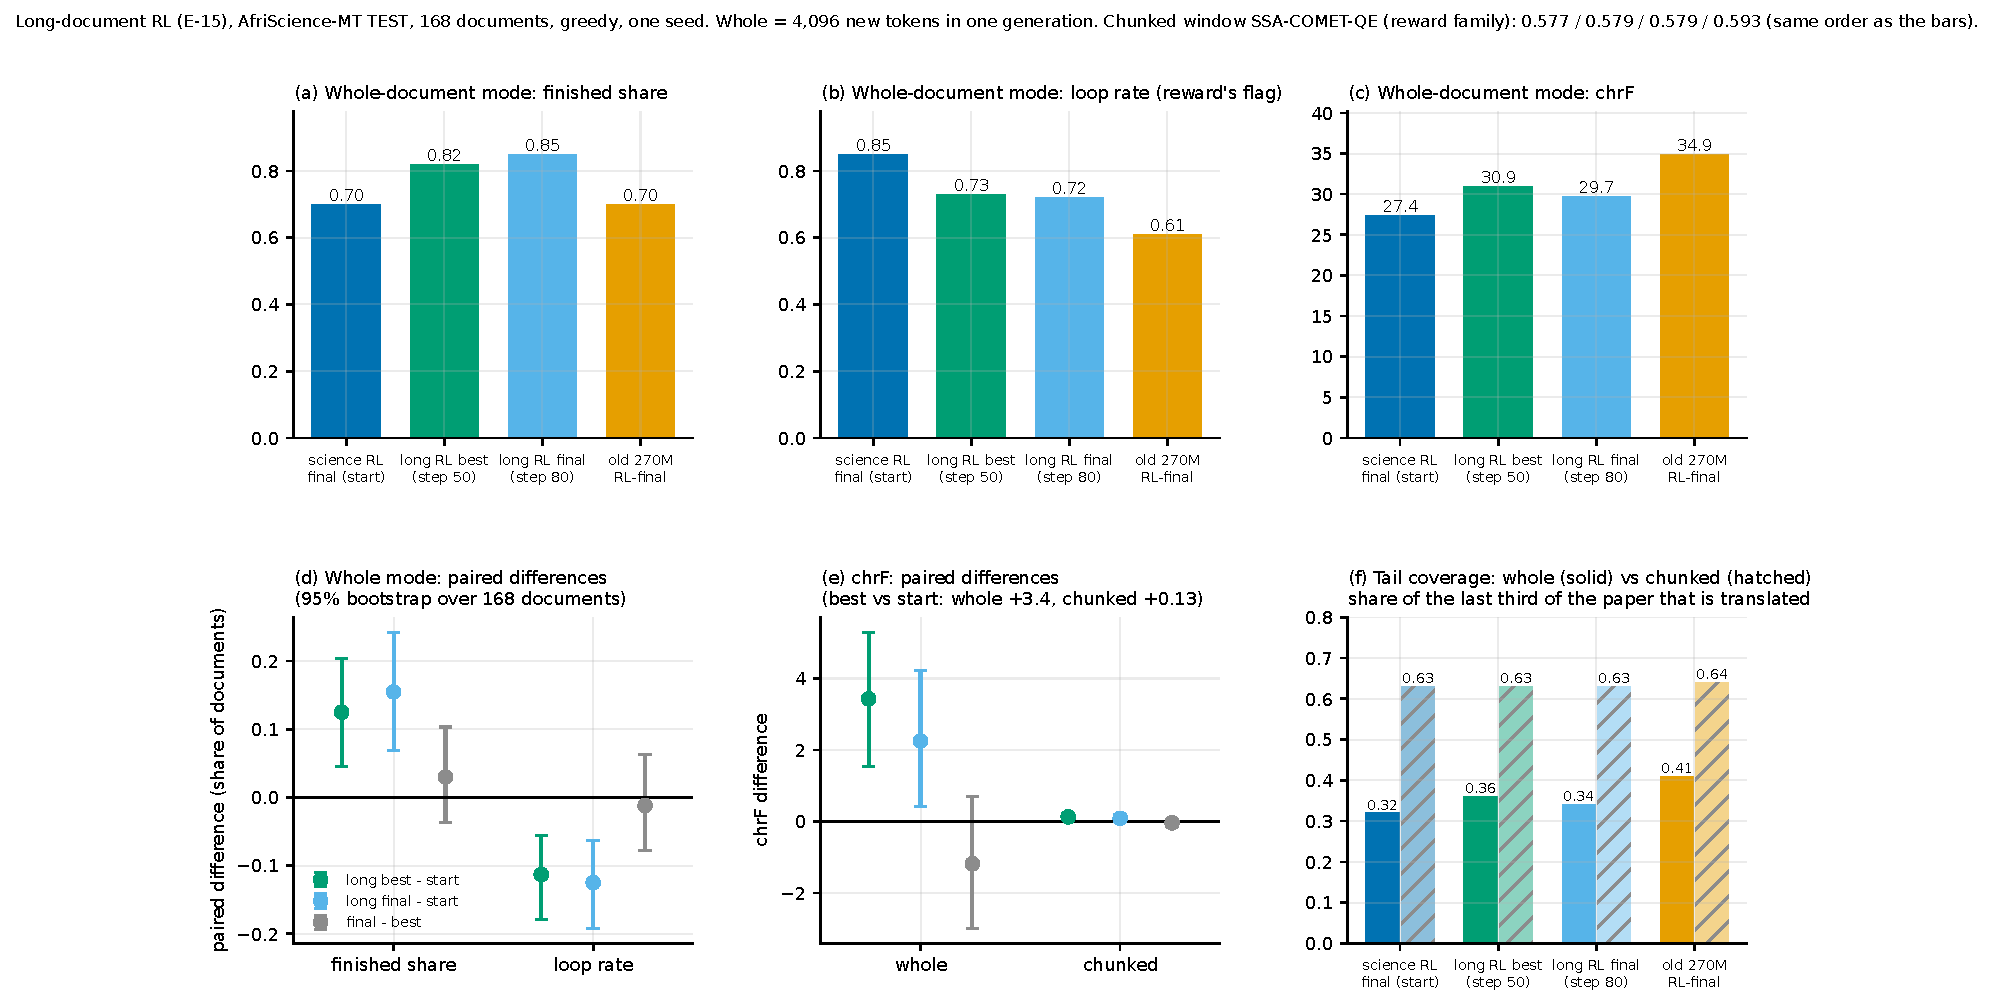
\includegraphics[width=1.00\linewidth]{figures/fig9_long_document_rl.pdf}
\caption{Long-document RL (E-15), AfriScience-MT TEST, 168 documents (28 papers $\times$ 6 languages), greedy, one seed. (a-c) Whole-document mode (4,096 new tokens in one generation): finished share, loop rate (the reward's flag) and chrF for the science RL final (the start), the long-document RL best (step 50) and final (step 80), and the earlier 270M work's 270M RL-final. (d, e) Paired differences with 95\% bootstrap over documents (Poisson weights): finished share, loop rate and chrF in whole mode, chrF in chunked mode. (f) Tail coverage, the share of the last third of the paper that is translated, whole against chunked mode. Chunked window SSA-COMET-QE (reward family) is in the figure title. Sources: \texttt{reports/\allowbreak{}data/\allowbreak{}eval\_\allowbreak{}long\_\allowbreak{}rl\_\allowbreak{}2026-\allowbreak{}11-\allowbreak{}04/\allowbreak{}\{doc\_\allowbreak{}tables.\allowbreak{}md,doc\_\allowbreak{}pairs.\allowbreak{}json\}}.}\label{fig:fig9_long_document_rl}
\end{figure}

\section{Contamination audit and follow-ups}\label{app:contam}

\textbf{6.4 Contamination.} The audit scanned both sides of 25,911,095 training samples (A0 packs and the six stage-B shards) against all benchmark rows: \textbf{no benchmark sentence of 3 or more words is in the training text}; FLORES+ devtest 0 of 54,648 rows, NTREX 120 of 47,928 (0.25\%), MAFAND 94 of 20,009 (0.47\%), SmolSent 45 of 38,833, GlotStoryBook 15 of 3,426, all one- or two-word strings; the FLORES+ dev train half is found in 23,706 of 23,760 rows (positive control); \texttt{all}, \texttt{clean}, \texttt{no\_\allowbreak{}pair} and \texttt{clean\_\allowbreak{}strict} macros agree within 0.01 chrF++. 
% src: reports/contamination_audit_385m_2026-11-03.md sections 1, 3, 6; reports/eval_385m_results_2026-11-03.md section 0

\emph{Follow-ups (CPU, 2026-11-04).} 
% src: CFU sections 0-6

\begin{itemize}
\item \textbf{Phrase level.} A lexical fuzzy scan of 56,975,939 pair rows and 4,277,612 instruction rows (reachable pair and instruction files, before gating and packing) finds no benchmark string of 8 or more tokens as a contiguous run. Strings of 4 to 7 tokens do occur inside longer training text (English side: MAFAND 134 of 17,428 strings, GlotStoryBook 30 of 898, NTREX 18 of 1,973, SALT 12 of 498; FLORES+ devtest, SmolSent, IbomMT and FLORES-MOZ 0); the audit's run rule and the intake filter test such short strings only for whole-sentence equality, so ``no benchmark sentence of 3 or more words'' holds for whole sentences, not for phrases. 263 (string, benchmark) cases of 8+ token English strings have a character-5-gram Jaccard $\ge$ 0.5 with some training text (MAFAND 184, SALT 27, NTREX 19, GlotStoryBook 15, SmolSent 6, FLORES+ devtest 4 of 1,012). These are candidates, not proof of leakage; their effect on scores was not measured.
\item \textbf{Prompts of the RL.} Stage A drew 6 flagged prompts of 28,120 (0.021\%); 6 of 1,345 prompts drawn for the seven languages whose prompt files had not been filtered (0.45\%), all distinct, in steps 72-364, source side only (this replaces the earlier estimate of about 0.15\%). The pool of the long-document RL (241,679 rows) has 0 rows flagged by the protected index.
\item \textbf{AfriScience-MT train versus the SFT text.} 305 of 34,007 train rows (0.9\%; hau 64, yor 116, zul 125) have their African-language sentence verbatim in the A0 pair data, all from \texttt{HuggingFaceFW/\allowbreak{}finetranslations}; 3 rows (yor 2, zul 1) as a pair. The packed shards were not scanned. The test papers are untouched (0 of 5,820 rows).
\item \textbf{A0 text.} The files support that A0's pack set is the first 138,873 packs of the audited g0 (identical per-language pack counts for 84 languages); pack content was not hash-compared.
\item \textbf{Not covered:} embedding or MT-round-trip paraphrase contamination, Gemma-3 pretraining, packed-shard coverage of the AfriScience train overlap and of the phrase scan (not run: these scans need the data box; Appendix~\ref{app:limits} item 15).
\end{itemize}

Benchmarks were evaluated many times; checkpoint choice used only the dev set (Appendix~\ref{app:limits}).

\section{NLLB-mined data and the regression against the earlier 270M work}\label{app:nllblink}

All 17 languages more than 5 chrF++ below the old SFT were already below with A0 (no NLLB-mined rows); the mean gap old SFT to A0 is \ensuremath{-}10.7 and A0 to 385M SFT +2.1; Venda (no NLLB rows) regressed \ensuremath{-}9.7. Spearman of NLLB share with the regression: \ensuremath{-}0.45 [\ensuremath{-}0.73, \ensuremath{-}0.09] on NTREX+MAFAND clean (n = 28), \ensuremath{-}0.07 [\ensuremath{-}0.35, +0.20] on the pooled index (n = 57), \ensuremath{-}0.17 [\ensuremath{-}0.54, +0.23] after RL. Each factor of 10 in NLLB-mined tokens adds \ensuremath{-}0.4 chrF++ (bootstrap 95\% [\ensuremath{-}11.0, +4.8]) against +9.6 for other new tokens. NLLB-mined rows are noisier than the same language's other rows (GlotLID acceptance median 0.77 against 0.99; AfriCOMET-QE below the language median in 38 of 43 languages). The decisive ablation (about 34 A100-hours) was not run [skipped by the authors; E-17]. The regression of Appendix~\ref{app:family} gives the same ambiguity: the NLLB-mined share is positively related to the RL gain and negatively to the SFT level, both through the low-resource tail. 
% src: reports/nllb_regression_link_2026-11-03.md; FAMILY section 4; the numbers of NLLBLINK were not independently re-run

\section{Negative results}\label{app:neg}

\begin{itemize}
\item Weak-group RL (Section~\ref{sec:seeds}), science SFT on the headline metric (Section~\ref{sec:science}), whole-document decoding (Section~\ref{sec:science}), RL on the Arabic dialects and Tamazight (outside the prompt pool; English output rises, Section~\ref{sec:degen}).
\item Post-editor: an SFT post-editor applied to every sentence lowers chrF++ (FLORES+ \ensuremath{-}0.01 [\ensuremath{-}0.11, +0.10], NTREX \ensuremath{-}0.58 [\ensuremath{-}0.75, \ensuremath{-}0.41], MAFAND \ensuremath{-}0.93 [\ensuremath{-}1.14, \ensuremath{-}0.74], SmolSent \ensuremath{-}0.37 [\ensuremath{-}0.52, \ensuremath{-}0.24]); restricted to the 3.9\% of drafts that are empty, unfinished or loops it gains +0.70 [+0.63, +0.78] chrF++ on FLORES+ but leaves AfriCOMET and SSA-COMET unchanged (\ensuremath{-}0.0007 to +0.0009), and beam-4 is stronger. 
% src: reports/post_editor_run_2026-11-03.md section 0
\end{itemize}

\section{Metric independence: full table}\label{app:indep}

\begin{table}[t]
\centering\footnotesize
\setlength{\tabcolsep}{4pt}
\caption{Metric independence (full). IND = not in any reward; RWD = in the reward; LOOP = optimised by construction.}\label{tab:indep_full}
\begin{tabularx}{\linewidth}{@{}>{\raggedright\arraybackslash}X>{\raggedright\arraybackslash}X>{\raggedright\arraybackslash}X@{}}
\toprule
metric & in the RL reward? & use in this paper \\
\midrule
\texttt{masakhane/\allowbreak{}africomet-\allowbreak{}qe-\allowbreak{}stl-\allowbreak{}1.\allowbreak{}1} (reference-free) & yes & not used as evidence \\
\texttt{McGill-\allowbreak{}NLP/\allowbreak{}ssa-\allowbreak{}comet-\allowbreak{}mtl} (reference-free; reference-based in the science RL) & yes & not used as evidence of RL gains \\
\texttt{McGill-\allowbreak{}NLP/\allowbreak{}ssa-\allowbreak{}comet-\allowbreak{}qe} (AfriScience-MT headline) & no, but the same family as the reward member & headline for SFT-only comparisons; for RL models shown only next to plain chrF and held-out AfriCOMET (all stages in Section~\ref{sec:science}) \\
TranslatePsy quality filters (AfriCOMET, SSA-COMET, MetricX) & not a reward; they filtered the training data of the E-03 control & neural metrics favour the control; chrF and chrF++ are the evidence (Section~\ref{sec:control}) \\
consensus utility (sample agreement in chrF++) & yes & chrF++ gains are partly in the optimised family \\
NLLB-3.3B pseudo-reference chrF++ & yes, 5 languages (kea kbp nus bam kab) & chrF++ on those 5 languages is not independent; relevant to the NLLB comparison (Section~\ref{sec:nllb}) \\
chrF++ against a human reference, weight 0.35 & yes, 7 languages (reference rows only; AfriScience TRAIN pairs) & chrF++ on those 7 languages can be partly trained; the test sets differ \\
language-ID, copy, repetition, length, end-of-turn guards & yes & finished and loop rates are optimised by construction \\
independent degeneration detector (lzma residual, repeated character 8-grams, repeated word 3-grams; thresholds from the 0.1\% tail of human references) & no & measures the same idea as the loop guard with different code and constants (Section~\ref{sec:rlsft}) \\
NLLB-218 language identification (\texttt{facebook/\allowbreak{}fasttext-\allowbreak{}language-\allowbreak{}identification}) & no & independent check of the language guard; evaluation use only (cc-by-nc-4.0) \\
\texttt{masakhane/\allowbreak{}africomet-\allowbreak{}stl-\allowbreak{}1.\allowbreak{}1} (reference-based) & no (held out; monitor and alarm) & the independent neural check; same family as the QE member \\
chrF / chrF++ / spBLEU against human references of the benchmarks & no & the main lexical evidence \\
\bottomrule
\end{tabularx}
\end{table}

% src: reports/rl_vs_sft_evidence_2026-11-04.md section 1; reports/eval_science_sft_385m_2026-11-04.md Goodhart caution; DEGEN section 1

\section{Per-language tables}\label{app:perlang}

\begin{figure}[t]
\centering
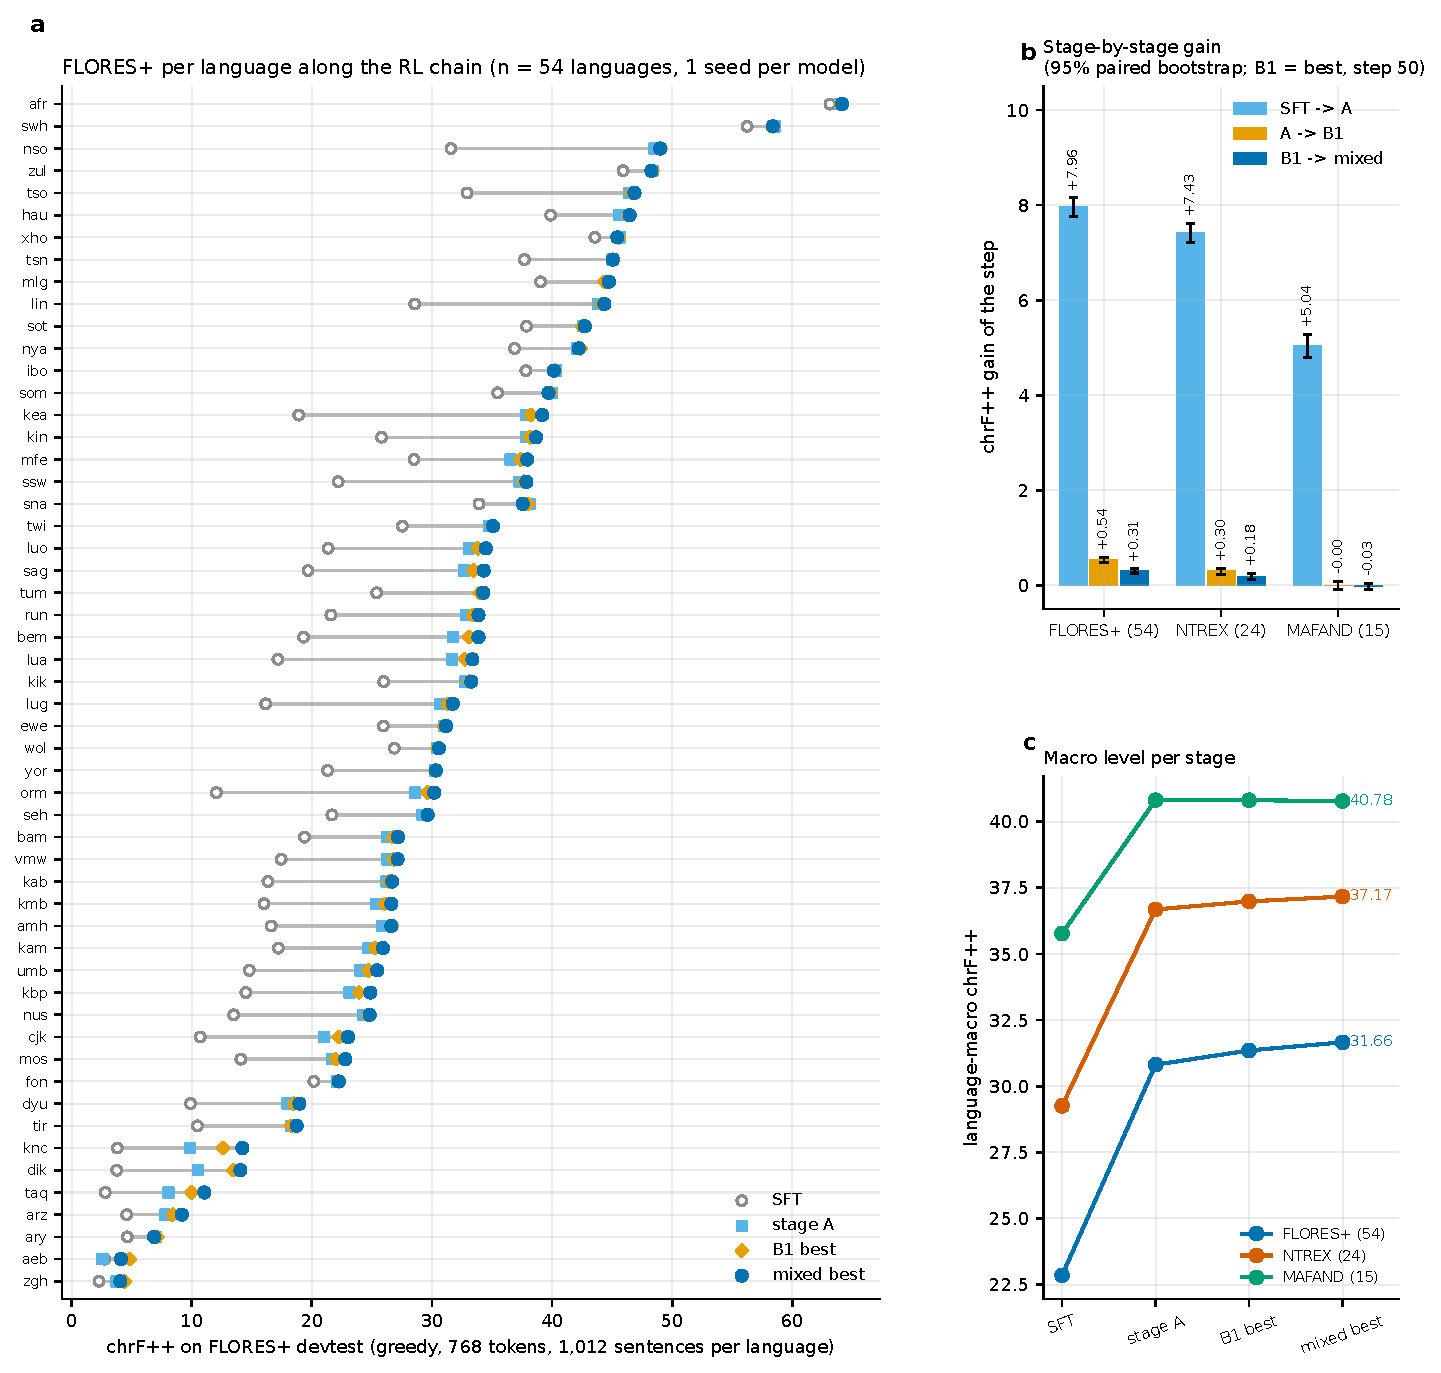
\includegraphics[width=0.95\linewidth]{figures/fig1_flores_per_language.pdf}
\caption{(a) FLORES+ devtest chrF++ per language (n = 54 languages, 1,012 sentences each; greedy, 768 tokens) for the SFT (open circle), RL stage A (square), B1 best (step 50, diamond) and the mixed best (filled circle), sorted by the mixed best; one training seed per model. (b) Gain of each RL step (language macro, 95\% paired bootstrap over sentences, Poisson weights shared across parallel languages) on FLORES+ (54 languages), NTREX (24) and MAFAND (15). (c) Language-macro chrF++ after each stage. Sources: \texttt{reports/\allowbreak{}data/\allowbreak{}eval\_\allowbreak{}weak\_\allowbreak{}group\_\allowbreak{}2026-\allowbreak{}11-\allowbreak{}03/\allowbreak{}results/\allowbreak{}results\_\allowbreak{}\{sft,stageA,b1best,mixedbest\}.\allowbreak{}csv}, \texttt{reports/\allowbreak{}data/\allowbreak{}rl\_\allowbreak{}vs\_\allowbreak{}sft\_\allowbreak{}evidence\_\allowbreak{}2026-\allowbreak{}11-\allowbreak{}04/\allowbreak{}evidence.\allowbreak{}json}.}\label{fig:fig1_flores_per_language}
\end{figure}

Sources: \texttt{reports/data/rl\_vs\_sft\_evidence\_2026-11-04/tables.md} (Tables 6, 7a, 7b) and \texttt{reports/data/nllb\_comparison\_rl\_models\_2026-11-04/table2\_per\_language\_43.csv}. Intervals are 95\% paired bootstrap over sentences (Poisson weights, 1,000 resamples); NLLB columns are published values.

{\scriptsize
\setlength{\tabcolsep}{4pt}
\begin{longtable}{@{}lrrllll@{}}
\caption{RL minus SFT per language on FLORES+ devtest (54 languages, all rows; \chrfpp{}). Finished / loop are the reward's flags; ``paired keeps rows where both models finished and neither loops.}\label{tab:perlang_flores}\\
\toprule
iso & SFT & RL & $\Delta$ all rows [CI] & SFT finished / loop & RL finished / loop & $\Delta$ paired rows [CI] \\
\midrule\endfirsthead
\toprule
iso & SFT & RL & $\Delta$ all rows [CI] & SFT finished / loop & RL finished / loop & $\Delta$ paired rows [CI] \\
\midrule\endhead
\bottomrule\endlastfoot
kea & 18.91 & 39.18 & +20.27 [+18.91, +21.53] & 0.83 / 0.20 & 1.00 / 0.00 & +7.66 [+6.93, +8.42] \\
orm & 12.06 & 30.18 & +18.12 [+17.49, +18.76] & 0.59 / 0.45 & 1.00 / 0.00 & +2.99 [+2.51, +3.50] \\
nso & 31.58 & 49.01 & +17.43 [+15.75, +19.09] & 0.86 / 0.15 & 1.00 / 0.00 & +4.22 [+3.62, +4.91] \\
lua & 17.18 & 33.37 & +16.19 [+15.21, +17.13] & 0.85 / 0.25 & 1.00 / 0.00 & +5.45 [+4.94, +6.03] \\
lin & 28.56 & 44.35 & +15.78 [+14.19, +17.22] & 0.90 / 0.13 & 1.00 / 0.00 & +5.27 [+4.69, +5.84] \\
ssw & 22.20 & 37.86 & +15.66 [+14.46, +16.85] & 0.87 / 0.17 & 1.00 / 0.00 & +5.38 [+4.85, +5.93] \\
lug & 16.17 & 31.73 & +15.57 [+14.66, +16.52] & 0.79 / 0.25 & 1.00 / 0.01 & +5.32 [+4.78, +5.87] \\
sag & 19.68 & 34.31 & +14.62 [+13.64, +15.55] & 0.87 / 0.20 & 1.00 / 0.00 & +5.99 [+5.51, +6.47] \\
bem & 19.31 & 33.88 & +14.56 [+13.63, +15.61] & 0.88 / 0.18 & 1.00 / 0.01 & +7.16 [+6.60, +7.75] \\
tso & 32.92 & 46.86 & +13.93 [+12.43, +15.51] & 0.91 / 0.11 & 1.00 / 0.00 & +4.45 [+3.82, +5.07] \\
luo & 21.36 & 34.49 & +13.13 [+11.91, +14.15] & 0.92 / 0.13 & 1.00 / 0.00 & +6.44 [+5.88, +6.95] \\
kin & 25.81 & 38.66 & +12.86 [+11.66, +14.03] & 0.89 / 0.12 & 1.00 / 0.00 & +5.66 [+5.09, +6.21] \\
cjk & 10.72 & 23.02 & +12.31 [+11.70, +12.89] & 0.71 / 0.31 & 1.00 / 0.01 & +2.13 [+1.86, +2.42] \\
run & 21.59 & 33.88 & +12.29 [+11.21, +13.15] & 0.88 / 0.15 & 1.00 / 0.01 & +5.03 [+4.52, +5.57] \\
nus & 13.49 & 24.82 & +11.32 [+10.73, +11.91] & 0.67 / 0.41 & 1.00 / 0.00 & +1.97 [+1.56, +2.36] \\
umb & 14.80 & 25.46 & +10.66 [+9.77, +11.44] & 0.89 / 0.15 & 1.00 / 0.01 & +4.84 [+4.43, +5.26] \\
kmb & 16.02 & 26.62 & +10.61 [+9.82, +11.37] & 0.88 / 0.23 & 1.00 / 0.00 & +3.93 [+3.56, +4.29] \\
knc & 3.81 & 14.22 & +10.41 [+9.95, +10.88] & 0.46 / 0.94 & 1.00 / 0.48 & +2.49 [+0.82, +3.99] \\
kbp & 14.51 & 24.88 & +10.37 [+9.70, +11.00] & 0.85 / 0.26 & 1.00 / 0.01 & +5.48 [+4.98, +5.94] \\
kab & 16.35 & 26.69 & +10.34 [+9.50, +11.14] & 0.84 / 0.20 & 1.00 / 0.00 & +2.26 [+1.92, +2.61] \\
dik & 3.76 & 14.06 & +10.30 [+9.75, +10.81] & 0.29 / 0.85 & 1.00 / 0.40 & +1.80 [+1.10, +2.60] \\
amh & 16.62 & 26.62 & +10.00 [+9.04, +10.96] & 0.87 / 0.13 & 1.00 / 0.00 & +2.80 [+2.29, +3.29] \\
vmw & 17.45 & 27.14 & +9.69 [+8.92, +10.48] & 0.84 / 0.18 & 1.00 / 0.00 & +2.11 [+1.81, +2.44] \\
mfe & 28.51 & 37.93 & +9.42 [+7.98, +10.94] & 0.94 / 0.07 & 1.00 / 0.01 & +3.91 [+3.43, +4.37] \\
dyu & 9.90 & 18.97 & +9.06 [+8.47, +9.62] & 0.83 / 0.25 & 1.00 / 0.00 & +4.11 [+3.80, +4.44] \\
yor & 21.32 & 30.33 & +9.01 [+7.99, +10.00] & 0.95 / 0.05 & 1.00 / 0.00 & +5.83 [+5.09, +6.56] \\
tum & 25.40 & 34.27 & +8.87 [+7.89, +9.79] & 0.94 / 0.08 & 1.00 / 0.00 & +4.57 [+4.08, +5.06] \\
kam & 17.22 & 25.92 & +8.70 [+7.93, +9.50] & 0.92 / 0.14 & 1.00 / 0.00 & +4.42 [+4.01, +4.83] \\
mos & 14.09 & 22.79 & +8.70 [+8.13, +9.33] & 0.90 / 0.19 & 1.00 / 0.01 & +4.54 [+4.17, +4.89] \\
tir & 10.48 & 18.74 & +8.26 [+7.69, +8.86] & 0.77 / 0.23 & 1.00 / 0.00 & +2.23 [+1.83, +2.66] \\
taq & 2.81 & 11.06 & +8.25 [+7.82, +8.67] & 0.14 / 0.91 & 0.99 / 0.56 & +3.27 [+1.81, +4.58] \\
seh & 21.67 & 29.65 & +7.98 [+7.00, +8.86] & 0.92 / 0.12 & 1.00 / 0.00 & +2.01 [+1.70, +2.33] \\
bam & 19.39 & 27.17 & +7.78 [+6.96, +8.59] & 0.89 / 0.13 & 1.00 / 0.00 & +2.47 [+2.14, +2.80] \\
twi & 27.54 & 35.07 & +7.53 [+6.47, +8.61] & 0.94 / 0.08 & 1.00 / 0.00 & +2.47 [+2.02, +2.92] \\
tsn & 37.69 & 45.05 & +7.36 [+6.18, +8.65] & 0.96 / 0.06 & 1.00 / 0.00 & +2.09 [+1.67, +2.59] \\
kik & 25.98 & 33.28 & +7.30 [+6.39, +8.22] & 0.93 / 0.08 & 1.00 / 0.00 & +3.32 [+2.89, +3.81] \\
hau & 39.88 & 46.46 & +6.58 [+5.09, +8.34] & 0.96 / 0.04 & 1.00 / 0.01 & +0.90 [+0.50, +1.30] \\
mlg & 39.04 & 44.73 & +5.68 [+4.54, +6.77] & 0.97 / 0.03 & 1.00 / 0.00 & +2.03 [+1.59, +2.45] \\
nya & 36.88 & 42.21 & +5.33 [+4.23, +6.54] & 0.97 / 0.04 & 1.00 / 0.00 & +1.82 [+1.41, +2.24] \\
ewe & 25.96 & 31.17 & +5.21 [+4.46, +6.04] & 0.95 / 0.06 & 1.00 / 0.00 & +2.12 [+1.75, +2.51] \\
sot & 37.87 & 42.72 & +4.85 [+3.70, +6.08] & 0.97 / 0.04 & 1.00 / 0.00 & +1.15 [+0.82, +1.50] \\
arz & 4.59 & 9.18 & +4.59 [+4.01, +5.15] & 0.49 / 0.52 & 0.87 / 0.19 & +0.67 [+0.05, +1.25] \\
som & 35.47 & 39.71 & +4.24 [+3.14, +5.34] & 0.97 / 0.03 & 1.00 / 0.00 & +1.38 [+1.02, +1.75] \\
wol & 26.87 & 30.58 & +3.72 [+2.74, +4.63] & 0.97 / 0.03 & 1.00 / 0.00 & +1.14 [+0.82, +1.44] \\
sna & 33.92 & 37.56 & +3.64 [+2.47, +4.85] & 0.97 / 0.04 & 1.00 / 0.00 & +0.26 [\ensuremath{-}0.11, +0.66] \\
zul & 45.91 & 48.27 & +2.36 [+1.56, +3.14] & 0.99 / 0.01 & 1.00 / 0.00 & +1.26 [+0.84, +1.67] \\
ibo & 37.82 & 40.14 & +2.33 [+1.57, +3.08] & 0.98 / 0.02 & 1.00 / 0.00 & +0.88 [+0.53, +1.24] \\
ary & 4.64 & 6.88 & +2.24 [+1.76, +2.74] & 0.54 / 0.48 & 0.97 / 0.11 & \ensuremath{-}3.70 [\ensuremath{-}4.39, \ensuremath{-}3.03] \\
swh & 56.24 & 58.36 & +2.12 [+1.10, +3.38] & 1.00 / 0.01 & 1.00 / 0.00 & +0.88 [+0.45, +1.30] \\
fon & 20.17 & 22.25 & +2.07 [+1.60, +2.55] & 0.98 / 0.04 & 1.00 / 0.00 & +0.77 [+0.56, +0.97] \\
xho & 43.56 & 45.43 & +1.87 [+1.05, +2.80] & 0.99 / 0.01 & 1.00 / 0.00 & +0.67 [+0.28, +1.09] \\
zgh & 2.29 & 4.07 & +1.78 [+1.30, +2.30] & 0.12 / 0.89 & 0.97 / 0.46 & \ensuremath{-}6.69 [\ensuremath{-}9.11, \ensuremath{-}4.34] \\
aeb & 2.75 & 4.12 & +1.36 [+0.96, +1.78] & 0.53 / 0.49 & 0.96 / 0.25 & \ensuremath{-}2.46 [\ensuremath{-}3.19, \ensuremath{-}1.74] \\
afr & 63.13 & 64.13 & +1.01 [+0.53, +1.61] & 1.00 / 0.00 & 1.00 / 0.00 & +0.78 [+0.46, +1.11] \\
\end{longtable}
}

{\scriptsize
\setlength{\tabcolsep}{4pt}
\begin{longtable}{@{}lrrrll@{}}
\caption{RL minus SFT per language on NTREX (clean rows; \chrfpp{} and held-out AfriCOMET).}\label{tab:perlang_ntrex}\\
\toprule
iso & n & SFT chrF++ & RL chrF++ & $\Delta$ all rows [CI] & $\Delta$ AfriCOMET [CI] \\
\midrule\endfirsthead
\toprule
iso & n & SFT chrF++ & RL chrF++ & $\Delta$ all rows [CI] & $\Delta$ AfriCOMET [CI] \\
\midrule\endhead
\bottomrule\endlastfoot
orm & 1992 & 9.63 & 27.33 & +17.70 [+17.16, +18.25] & +0.168 [+0.161, +0.175] \\
ven & 1992 & 21.30 & 38.81 & +17.52 [+16.72, +18.31] & - \\
ssw & 1992 & 21.58 & 38.80 & +17.22 [+16.40, +18.02] & +0.122 [+0.115, +0.130] \\
bem & 1992 & 18.68 & 34.79 & +16.11 [+15.43, +16.84] & +0.111 [+0.105, +0.117] \\
nso & 1992 & 20.14 & 32.73 & +12.60 [+11.83, +13.35] & +0.101 [+0.095, +0.108] \\
tsn & 1992 & 36.97 & 48.71 & +11.74 [+10.68, +12.81] & +0.073 [+0.067, +0.080] \\
kin & 1992 & 26.40 & 37.13 & +10.73 [+9.95, +11.52] & +0.072 [+0.066, +0.078] \\
som & 1992 & 35.84 & 44.23 & +8.39 [+7.44, +9.25] & +0.061 [+0.055, +0.066] \\
yor & 1992 & 23.77 & 32.10 & +8.33 [+7.58, +9.10] & +0.104 [+0.097, +0.110] \\
tir & 1992 & 9.10 & 17.00 & +7.90 [+7.52, +8.25] & +0.144 [+0.136, +0.151] \\
amh & 1992 & 10.58 & 18.05 & +7.46 [+7.00, +7.93] & +0.078 [+0.071, +0.084] \\
ewe & 1992 & 24.28 & 31.58 & +7.30 [+6.64, +8.00] & +0.064 [+0.059, +0.069] \\
hau & 1992 & 42.15 & 48.57 & +6.42 [+5.24, +7.58] & +0.028 [+0.023, +0.034] \\
nya & 1992 & 37.87 & 44.23 & +6.36 [+5.46, +7.34] & +0.025 [+0.020, +0.030] \\
wol & 1992 & 25.29 & 30.37 & +5.08 [+4.34, +5.86] & +0.032 [+0.027, +0.037] \\
sna & 1992 & 34.25 & 39.23 & +4.99 [+4.17, +5.83] & +0.024 [+0.019, +0.029] \\
ibo & 1992 & 39.90 & 44.87 & +4.97 [+4.17, +5.82] & +0.028 [+0.024, +0.032] \\
nde & 1992 & 28.83 & 32.95 & +4.12 [+3.51, +4.74] & - \\
mlg & 1992 & 36.91 & 40.85 & +3.94 [+3.19, +4.74] & +0.026 [+0.021, +0.031] \\
swh & 1992 & 55.18 & 58.73 & +3.55 [+2.55, +4.54] & +0.017 [+0.012, +0.022] \\
zul & 1992 & 40.92 & 43.50 & +2.58 [+1.89, +3.29] & +0.015 [+0.010, +0.019] \\
xho & 1992 & 39.85 & 42.36 & +2.51 [+1.92, +3.16] & +0.013 [+0.009, +0.017] \\
afr & 1992 & 62.42 & 63.92 & +1.50 [+1.00, +2.15] & +0.016 [+0.012, +0.020] \\
shi & 1992 & 0.24 & 1.16 & +0.93 [+0.85, +1.02] & - \\
\end{longtable}
}

{\scriptsize
\setlength{\tabcolsep}{4pt}
\begin{longtable}{@{}lrrrll@{}}
\caption{RL minus SFT per language on MAFAND-MT (clean rows; \chrfpp{} and held-out AfriCOMET).}\label{tab:perlang_mafand}\\
\toprule
iso & n & SFT chrF++ & RL chrF++ & $\Delta$ all rows [CI] & $\Delta$ AfriCOMET [CI] \\
\midrule\endfirsthead
\toprule
iso & n & SFT chrF++ & RL chrF++ & $\Delta$ all rows [CI] & $\Delta$ AfriCOMET [CI] \\
\midrule\endhead
\bottomrule\endlastfoot
lug & 1500 & 26.97 & 39.57 & +12.60 [+11.60, +13.70] & +0.065 [+0.058, +0.071] \\
yor & 1550 & 23.47 & 33.45 & +9.98 [+9.15, +10.70] & +0.127 [+0.119, +0.133] \\
kin & 1005 & 36.51 & 46.41 & +9.90 [+8.70, +11.20] & +0.064 [+0.056, +0.073] \\
luo & 1500 & 22.95 & 32.62 & +9.67 [+8.76, +10.50] & +0.072 [+0.065, +0.079] \\
tsn & 1500 & 43.85 & 53.10 & +9.24 [+7.87, +10.70] & +0.045 [+0.039, +0.052] \\
amh & 1014 & 11.62 & 18.33 & +6.71 [+5.91, +7.46] & +0.061 [+0.052, +0.070] \\
twi & 1500 & 28.58 & 34.14 & +5.56 [+4.75, +6.29] & +0.042 [+0.037, +0.047] \\
nya & 1003 & 38.14 & 40.95 & +2.81 [+1.96, +3.71] & +0.009 [+0.002, +0.015] \\
sna & 1004 & 30.35 & 32.91 & +2.56 [+1.64, +3.39] & +0.018 [+0.011, +0.025] \\
xho & 1001 & 49.76 & 51.78 & +2.02 [+1.06, +2.98] & +0.008 [+0.002, +0.014] \\
ibo & 1458 & 43.55 & 44.89 & +1.34 [+0.43, +2.32] & +0.005 [+0.000, +0.010] \\
swh & 1822 & 50.68 & 51.79 & +1.12 [+0.38, +1.89] & +0.012 [+0.007, +0.017] \\
zul & 998 & 44.50 & 45.58 & +1.08 [+0.49, +1.73] & +0.011 [+0.005, +0.017] \\
hau & 1498 & 32.03 & 32.80 & +0.77 [+0.21, +1.41] & +0.014 [+0.009, +0.019] \\
pcm & 1562 & 53.58 & 53.34 & \ensuremath{-}0.25 [\ensuremath{-}0.69, +0.30] & +0.007 [+0.004, +0.009] \\
\end{longtable}
}

{\scriptsize
\setlength{\tabcolsep}{4pt}
\begin{longtable}{@{}llrrrrl@{}}
\caption{FLORES+ devtest \chrfpp{} on the 43 languages shared with the published NLLB table (our values greedy; NLLB-3.3B published). Yoruba: the published value is anomalously low.}\label{tab:perlang_nllb}\\
\toprule
iso & language & NLLB-3.3B & SFT & RL mixed best & mixed minus NLLB-3.3B & NLLB tertile \\
\midrule\endfirsthead
\toprule
iso & language & NLLB-3.3B & SFT & RL mixed best & mixed minus NLLB-3.3B & NLLB tertile \\
\midrule\endhead
\bottomrule\endlastfoot
yor & Yoruba & 24.90 & 21.32 & 30.33 & +5.43 & tail (15) \\
fon & Fon & 19.30 & 20.17 & 22.25 & +2.95 & tail (15) \\
dyu & Dyula & 16.20 & 9.90 & 18.97 & +2.77 & tail (15) \\
wol & Wolof & 28.10 & 26.87 & 30.58 & +2.48 & tail (15) \\
kam & Kamba & 23.60 & 17.22 & 25.92 & +2.32 & tail (15) \\
kmb & Kimbundu & 24.40 & 16.02 & 26.62 & +2.22 & tail (15) \\
umb & Umbundu & 23.60 & 14.80 & 25.46 & +1.86 & tail (15) \\
afr & Afrikaans & 64.70 & 63.13 & 64.13 & \ensuremath{-}0.57 & high (14) \\
ibo & Igbo & 41.10 & 37.82 & 40.14 & \ensuremath{-}0.96 & mid (14) \\
nso & Sepedi & 50.30 & 31.58 & 49.01 & \ensuremath{-}1.29 & high (14) \\
mos & Mossi & 24.10 & 14.09 & 22.79 & \ensuremath{-}1.31 & tail (15) \\
swh & Swahili & 60.00 & 56.24 & 58.36 & \ensuremath{-}1.64 & high (14) \\
lua & Luba-Kasai & 35.20 & 17.18 & 33.37 & \ensuremath{-}1.83 & tail (15) \\
sag & Sango & 36.50 & 19.68 & 34.31 & \ensuremath{-}2.19 & mid (14) \\
tum & Tumbuka & 36.60 & 25.40 & 34.27 & \ensuremath{-}2.33 & mid (14) \\
nya & Chichewa & 45.30 & 36.88 & 42.21 & \ensuremath{-}3.09 & high (14) \\
som & Somali & 42.80 & 35.47 & 39.71 & \ensuremath{-}3.09 & mid (14) \\
xho & Xhosa & 48.60 & 43.56 & 45.43 & \ensuremath{-}3.17 & high (14) \\
twi & Twi & 38.30 & 27.54 & 35.07 & \ensuremath{-}3.23 & mid (14) \\
tso & Tsonga & 50.20 & 32.92 & 46.86 & \ensuremath{-}3.34 & high (14) \\
tsn & Setswana & 48.60 & 37.69 & 45.05 & \ensuremath{-}3.55 & high (14) \\
bem & Bemba & 37.50 & 19.31 & 33.88 & \ensuremath{-}3.62 & mid (14) \\
lin & Lingala & 48.00 & 28.56 & 44.35 & \ensuremath{-}3.65 & high (14) \\
sot & Sesotho & 46.50 & 37.87 & 42.72 & \ensuremath{-}3.78 & high (14) \\
kik & Kikuyu & 37.30 & 25.98 & 33.28 & \ensuremath{-}4.02 & mid (14) \\
nus & Nuer & 28.90 & 13.49 & 24.82 & \ensuremath{-}4.08 & tail (15) \\
bam & Bambara & 31.40 & 19.39 & 27.17 & \ensuremath{-}4.23 & tail (15) \\
luo & Luo & 39.00 & 21.36 & 34.49 & \ensuremath{-}4.51 & mid (14) \\
kbp & Kabiye & 29.50 & 14.51 & 24.88 & \ensuremath{-}4.62 & tail (15) \\
zul & Zulu & 53.50 & 45.91 & 48.27 & \ensuremath{-}5.23 & high (14) \\
sna & Shona & 42.80 & 33.92 & 37.56 & \ensuremath{-}5.24 & mid (14) \\
kab & Kabyle & 32.00 & 16.35 & 26.69 & \ensuremath{-}5.31 & tail (15) \\
mlg & Malagasy & 50.20 & 39.04 & 44.73 & \ensuremath{-}5.47 & high (14) \\
orm & Oromo & 35.70 & 12.06 & 30.18 & \ensuremath{-}5.52 & tail (15) \\
ssw & Swati & 43.50 & 22.20 & 37.86 & \ensuremath{-}5.64 & mid (14) \\
hau & Hausa & 52.50 & 39.88 & 46.46 & \ensuremath{-}6.04 & high (14) \\
tir & Tigrinya & 24.80 & 10.48 & 18.74 & \ensuremath{-}6.06 & tail (15) \\
lug & Luganda & 38.50 & 16.17 & 31.73 & \ensuremath{-}6.77 & mid (14) \\
ewe & Ewe & 38.20 & 25.96 & 31.17 & \ensuremath{-}7.03 & mid (14) \\
run & Kirundi & 41.90 & 21.59 & 33.88 & \ensuremath{-}8.02 & mid (14) \\
kea & Kabuverdianu & 47.90 & 18.91 & 39.18 & \ensuremath{-}8.72 & high (14) \\
kin & Kinyarwanda & 48.40 & 25.81 & 38.66 & \ensuremath{-}9.74 & high (14) \\
amh & Amharic & 37.90 & 16.62 & 26.62 & \ensuremath{-}11.28 & mid (14) \\
\end{longtable}
}

\section{Limitations: full list}\label{app:limits}

The numbered list of Appendix~\ref{app:limits} is a compressed version of this one.

\begin{enumerate}
\item \textbf{Single training seed} for every model and stage; all intervals are test-sentence bootstrap (1,000 resamples; Poisson weights shared across parallel languages for the RL-versus-SFT claims), and some are over languages only (NLLB, family analysis). Evaluation noise of the dev macro is sd 0.09 to 0.10 chrF++; training-run variation was measured only for the stage-A recipe at 100 steps on 20 languages with one pair of extra seeds (E-04: 0.06 chrF++ [\ensuremath{-}0.02, +0.14] between the two; Appendix~\ref{app:split}); seeds of later stages, of the science and long-document stages and of the SFT are not available (a second SFT seed is impractical: stage B alone is 44.8 A100-hours). The mixed step (+0.31 on FLORES+; +0.07 on the 20 languages of the seed study) and per-language differences under about 0.5 chrF++ (pcm, hau, ibo) cannot be separated from seed noise.
\end{enumerate}
% GATE E-01 E-03
\begin{enumerate}
\item \textbf{The matched-compute control is one run.} E-03 (Section~\ref{sec:control}) has one seed, one learning rate (the pre-registered probe's best of three), one data mix (50\% replay + 50\% TranslatePsy for 19 languages, with NLLB-3.3B targets) and \textbf{one evaluated budget point (6,000 steps)}: the stage-A-matched (3,100) and mixed-best-matched (4,800) checkpoints exist but were not evaluated, at the authors' request. Its registered verdict is ``inconclusive'' and was not changed. The decode-time loop-guard control (E-01) is reported in Section~\ref{sec:rlsft}, with the caveats that its best setting was the grid edge and that a stronger penalty was explored only on dev.
\item \textbf{No human judgement of system outputs} (E-10: not run; it needs native-speaker annotators, which the authors cannot commission, and no LLM-judge substitute was validated). All evidence is automatic; the neural checks are of one family, and AfriCOMET has a length/entity bias (shown next to chrF++, never alone). One reference per sentence.
\item \textbf{Reward-family overlap.} Finished, loop and language-ID rates are optimised by construction; SSA-COMET-QE (the AfriScience-MT headline) is a checkpoint of the reward's family; chrF++ is partly optimised through the consensus utility and, for 5 + 7 languages, through the NLLB and human-reference terms. The reward's own loop flag undercounts degeneration by 1.77 on FLORES+ (Section~\ref{sec:degen}), and the independent detector shares the repetition concept and is blind to non-repetitive failure.
\item \textbf{Ablations are limited} (E-11): three arms (no features, no reference domain, no beam guide) at 100 steps of the b64 recipe, one run per arm, sharing a 40-step prefix with seed 2, 20 languages, one pair of seeds as the noise yardstick; the KL-guard arm was not run (the guard never fired); dynamic sampling and the std floor alone, the reward components other than the reference term, and the later stages were not ablated; the mid-run changes of Appendix~\ref{app:disc} mean the stages are not a clean single design.
\end{enumerate}

\begin{enumerate}
\item \textbf{Metric choices changed after the fact for the science analysis}: the headline moved from reference-based SSA-COMET-MTL to reference-free SSA-COMET-QE after a calibration on released sentence-level runs only; the paper's own checkpoint is unverified.
\item \textbf{Engine and decoding.} The bf16 engine parity gate was not met (9.6\% identical outputs vLLM bf16 against HF bf16; chrF++ 36.22, 36.80, 38.18 on 240 sentences); E-09 shows the engines agree in fp32 (98.8\% and 97.1\% identical outputs for the SFT and the RL model), so the gate failure is bf16 rounding. E-09b: the SFT in fp32 on the full set differs from bf16 by \ensuremath{-}0.04 chrF++ [\ensuremath{-}0.13, +0.07] over 93 cells, so the bf16 headline does not overstate the RL gain; the earlier +0.24 to +1.81 range is superseded. Not done: the RL model in fp32 and AfriCOMET scoring of the fp32 SFT run. All headline numbers are vLLM 0.32.0 bf16 greedy at 768 tokens. Beam-4 and MBR-16 were measured at 768 tokens (E-02) on the SFT and the RL model only, on 20 languages $\times$ 200 sentences, with one SFT and one RL checkpoint, chrF++ as the MBR utility (metric-matched), a primary beam definition amended after a smoke test and before any score (stop at 4 ended hypotheses), and a second beam rule that gives a different sign for the RL model; the earlier 256-token beam numbers used a loop that ran past the end token and are not comparable.
\item \textbf{Language coverage.} 51 of 125 registry languages have no reference test and are unscored; many weak languages rest on one benchmark of 48 to 1,012 sentences; the family analysis covers 54 languages. The model fails on Arabic dialects, Tamazight, Dinka, Tamasheq and Kanuri, and RL increases English output there.
\item \textbf{Comparisons.} The old-versus-385M comparison (E-13, same harness, rows clean for both generations) is still a composite of data, steps, tokenizer layout and reward, with FLORES+ reduced to 4.7\% of its rows; the NLLB comparison uses FLORES-200 published numbers against FLORES+, beam against greedy and language-level intervals; AfriqueLLM numbers come from a different few-shot harness; bidirectional aggregates are not compared.
\item \textbf{Documents.} 28 papers per language (168 documents; the document intervals of the long-document RL are bootstrap over documents and reflect paper sampling only; the other document tables have no bootstrap); whole-document decoding was tested at 4,096 new tokens and remains unusable after the long-document RL (72 to 73\% loops); COMET encoders read 512 tokens, so only 4-sentence-window values are document scores; the 385M RL stages trained on prompts of at most 256 source tokens before the long-document RL.
\item \textbf{Cost and scale.} One 385M model and one language registry; A100 hours as in Section~\ref{sec:method}; no scaling claim.
\item \textbf{Unresolved and unevaluated items.} B1 final (step 135) was evaluated after the fact (E-20, \texttt{reports/\allowbreak{}e20\_\allowbreak{}b1\_\allowbreak{}final\_\allowbreak{}2026-\allowbreak{}11-\allowbreak{}04.\allowbreak{}md}): it equals B1 best (step 50) within noise (+0.01 chrF++ [\ensuremath{-}0.02, +0.04], AfriCOMET +0.0004 over 93 cells; the 85 later steps changed nothing measurable), and the mixed stage is +0.26 [+0.22, +0.30] chrF++ over B1 final on FLORES+; the NLLB-data ablation was not run [E-17]; sentence-paired comparison with NLLB on the full devtest was not run [E-06b].
\item \textbf{Not run:} human evaluation (needs native-speaker annotators); the packed-shard contamination scans, the content check of A0 against g0, the embedding and MT round-trip paraphrase scans and the source of the other 34 dev-train-half languages (need the data box); the NLLB-data ablation (skipped by the authors); beam widths other than 4, length penalties and the 54-language decoding run; a science SFT at alpha 1.0 followed by RL, a second seed of E-14 and a long-document RL from the E-14 model.
\end{enumerate}

\section{Disclosures: full statement}\label{app:disc}

Rule: data and signals that were actually used are stated, including those that are non-commercial or NLLB-derived. \texttt{DISCLOSURES.\allowbreak{}md} is the source of this section and holds the full tables. 
% src: DISCLOSURES sections 1-6; claims IDs L1-L5, CT1-CT13, CTL1-CTL6

\subsection{Training data and licences}


\begin{itemize}
\item \textbf{NLLB-derived share of the SFT.} NLLB-mined bitext (OPUS-NLLB, 43 languages, 13.46 M rows, plus a Fulah NLLB-mined set of 0.45 M rows) is \textbf{14.4\% of the 3.990 B stage-B pack tokens} (13.3\% of the 4.109 B executed; 10.84\% of the 5.043 B tokens drawn in the whole SFT); adding NLLB-Seed (tzm) and the aligned part of the Aya collection (NLLB-3.3B outputs; 169 M tokens in 12 languages) gives \textbf{18.7\%} (746 M tokens; executed 17.2\%; 14.36\% of the whole SFT); adding the machine-translated Tumbuka instruction sets (system not stated, possibly NLLB) gives \textbf{22.8\%} (909 M tokens; 17.86\% of the whole SFT). By rows, 13.91 M of 42.31 M stage-B translation pairs (32.9\%) are NLLB-mined. A0 contains none of the three. The authors allowed NLLB-mined rows with a per-language cap of 150k, ODC-BY with special attribution. NLLB models and outputs carry CC-BY-NC terms and the authors cannot use NLLB for production translation; a licence statement must accompany any release of the 385M weights. Not counted and needing a legal decision: the \texttt{*\_\allowbreak{}mt560} OPUS sets (69\% of the main pair output of the clean rebuild, 16.2 M of 23.4 M pairs, mostly Jehovah's Witnesses and Bible text, licence unknown, labelled NLLB-derived by an old converter docstring); \texttt{African-\allowbreak{}Languages-\allowbreak{}Lab/\allowbreak{}multi-\allowbreak{}open} (3,748,964 pairs, ``license: other''); AfroLingu-MT (gated, authors' exception); other machine-translated instruction sets with unstated systems (\texttt{african\_\allowbreak{}ultrachat}, \texttt{kiya\_\allowbreak{}sft}, \texttt{alpaca\_\allowbreak{}*}, \texttt{amharic\_\allowbreak{}*}); all four families are in the instruction pack stream (\texttt{packed\_\allowbreak{}instr}: every source of the instruction intake except \texttt{muri\_\allowbreak{}it}, 4,190,976 samples, 1.232 B tokens; \texttt{reports/\allowbreak{}intake2\_\allowbreak{}instr\_\allowbreak{}packs\_\allowbreak{}2026-\allowbreak{}11-\allowbreak{}01.\allowbreak{}md}); \texttt{african\_\allowbreak{}ultrachat} is UltraChat machine-translated into 11 languages, \texttt{alpaca\_\allowbreak{}*} (twi, swh, zul, wol, som) are translated Alpaca sets, \texttt{amharic\_\allowbreak{}*} and \texttt{kiya\_\allowbreak{}sft} (om, yo, sw, am rows) are machine-translated sets, and the translation system is not stated in the dataset cards or in the intake records; the packs carry no source field, so the tokens of each source drawn in stage B are not recorded. 
% src: NLLBLINK Licence-disclosure figure; HYG X10; REBUILD section 9; DISCLOSURES 1.1
\item \textbf{Unspecified-licence sources} in the main output: KwekuAinoo/eng\_twi 551,358; sentence-transformers/parallel-sentences-opus-100 210,479; UBC-NLP/AfroLingu-MT 207,796; cibfaye/wolof-english-bible 11,415; webfaq\_v2; bambara\_lm\_qa (381k, 83\% of Bambara instruction rows). Religious text dominates many low-resource languages (28 of the 81 RL languages are religious-only in the post-editor selection); the Efik NT sheet (7,936 verse pairs) has unconfirmed provenance and licence.
\item \textbf{IbomMT} is CC-BY-NC-4.0: a disclosed non-commercial exception in the SFT (once) and a human-reference source of the RL reference domain (efi, ibb).
\item \textbf{Quarantined and not used:} \texttt{yigagilbert/\allowbreak{}synthetic-\allowbreak{}parallel-\allowbreak{}external}, \texttt{fiifinketia/\allowbreak{}pristine-\allowbreak{}twi-\allowbreak{}english}, \texttt{muri-\allowbreak{}it}, the Aya parallel pairs.
\item \textbf{Gemma base model:} \texttt{google/\allowbreak{}gemma-\allowbreak{}3-\allowbreak{}270m-\allowbreak{}it}; the Gemma terms of use apply to the derived weights; pretraining text is unknown, so exposure of benchmarks through pretraining cannot be excluded.
\item \textbf{FLORES+ dev train half} (440 ids; 23,706 of 23,760 rows found in the audit) is in the SFT on purpose; the held-out half (557 ids) is protected.
\end{itemize}

\subsection{RL prompts and reward-side data}


\begin{itemize}
\item General prompts: FineWeb-Edu (ODC-By) and Wikipedia (CC BY-SA). News prompts (30\% of the draw): BBC News 2017-2025 (\texttt{RealTimeData/\allowbreak{}bbc\_\allowbreak{}news\_\allowbreak{}alltime}, \textbf{no licence declared, BBC copyright}), \texttt{permutans/\allowbreak{}c4-\allowbreak{}bbc-\allowbreak{}news} (ODC-By label inherited from C4, BBC copyright applies), Wikinews (CC BY 2.5), Global Voices (CC BY 3.0 per the sister card), Wikivoyage (CC BY-SA 4.0; 188 prompts drawn in stage A) and \texttt{SetFit/\allowbreak{}bbc-\allowbreak{}news} (37 pool rows, none drawn, licence not recorded). The prompts are RL \textbf{input} text only; the source is never a training target.
\item Seven new-language prompt files of stage A (\texttt{tll mfe guw lub crs zne lue}) had not been filtered; stage A drew 6 flagged prompts of 28,120 (0.021\%), 6 of 1,345 for those languages, source side only. B1 was restarted from its step-20 checkpoint with the filtered pool.
\item Reference domain (stage A from step 41, B1, mixed, science RL): human pairs from AfriScience-MT \textbf{train} (Apache-2.0; amh hau lug nso yor zul) and IbomMT train (CC-BY-NC-4.0; efi, ibb), anchors for 7 languages only. Test papers are in no pool. 0.9\% of the AfriScience train rows have their African-language sentence in the A0 pair data (Appendix~\ref{app:contam}).
\item \textbf{NLLB-3.3B pseudo-references (CC-BY-NC) are a reward signal} for kea kbp nus bam kab (weight 0.25, max 0.35), reward only; no NLLB text is a training target in RL.
\item Reward models: \texttt{masakhane/\allowbreak{}africomet-\allowbreak{}qe-\allowbreak{}stl-\allowbreak{}1.\allowbreak{}1}, \texttt{McGill-\allowbreak{}NLP/\allowbreak{}ssa-\allowbreak{}comet-\allowbreak{}mtl}; held-out monitor \texttt{masakhane/\allowbreak{}africomet-\allowbreak{}stl-\allowbreak{}1.\allowbreak{}1} (apache-2.0 verified); GlotLID language guard. Licences as declared on the Hub (read 2026-11-05): \texttt{McGill-\allowbreak{}NLP/\allowbreak{}ssa-\allowbreak{}comet-\allowbreak{}mtl} and \texttt{ssa-\allowbreak{}comet-\allowbreak{}qe} apache-2.0; \texttt{masakhane/\allowbreak{}africomet-\allowbreak{}qe-\allowbreak{}stl-\allowbreak{}1.\allowbreak{}1} apache-2.0; \texttt{cis-\allowbreak{}lmu/\allowbreak{}glotlid} \texttt{license: other} with \texttt{license\_\allowbreak{}name: apache-\allowbreak{}2.\allowbreak{}0-\allowbreak{}plus-\allowbreak{}notices} (card: Apache License 2.0 plus notices).
\item Science stages: science RL prompts \texttt{clean\_\allowbreak{}sci\_\allowbreak{}v2} (PMC, arXiv CC BY/CC0, AfriScience-MT train English); \textbf{LibreTexts was excluded} from the science RL (licence conflict CC BY against CC BY-NC-SA, 10,257 prompts). \textbf{LibreTexts is not absent from the long-document RL pool}: 3,428 \texttt{common-\allowbreak{}pile/\allowbreak{}libretexts} rows (17.8\% of \texttt{science\_\allowbreak{}b2048}). The rows were removed before the stage started; the long-document RL did not use them. The E-14 run (science RL started from the mixed best) used the same pool and reward as the executed science RL. Science SFT: AfriScience-MT train (Apache-2.0; 28,750 windows) plus replay cut from the general SFT shards (so the NLLB, Aya and Tumbuka shares apply to the replay); 54 further catalogue candidates were scanned and none used.
\end{itemize}

\subsection{TranslatePsy: used only in a research control}


\texttt{qvac/\allowbreak{}TranslatePsy-\allowbreak{}AfriSLM-\allowbreak{}Synthetic-\allowbreak{}Mix} (Gritta et al.; CC-BY-NC-4.0; targets are \texttt{facebook/\allowbreak{}nllb-\allowbreak{}200-\allowbreak{}3.\allowbreak{}3B} translations of MADLAD-400 sentences, filtered by AfriCOMET, SSA-COMET and MetricX) was authorised by the authors on 2026-11-04 \textbf{for the matched-compute continued-SFT control (E-03) only}. Its English-to-X rows (19 languages: afr amh hau ibo kin lin lug mlg nya orm sna som sot swh tsn wol xho yor zul) enter that control run, scanned against the protected index (any hit on either side removed; 0.67\% of the 950,000-row sample); \textbf{no TranslatePsy row is in the SFT, any RL stage, the science or long-document stages, or any released weight.} The control checkpoints are research artefacts (CC-BY-NC-4.0 and NLLB terms), are not pushed to any public repository and are not used in production. The comparison RL against control must state two things: the TranslatePsy quality filters are the reward family of the RL, so neural metrics favour the control while chrF and chrF++ do not; and TranslatePsy targets are NLLB-3.3B-like, so a good control result partly means ``distilling NLLB''. Status: run (preparation \texttt{reports/\allowbreak{}sft\_\allowbreak{}control\_\allowbreak{}prep\_\allowbreak{}2026-\allowbreak{}11-\allowbreak{}04.\allowbreak{}md}; execution record and result \texttt{reports/\allowbreak{}e03\_\allowbreak{}sft\_\allowbreak{}control\_\allowbreak{}2026-\allowbreak{}11-\allowbreak{}05.\allowbreak{}md}): 277,900 pairs per language for the 19 languages (5.28 M pairs, 96,138 packs, each seen once) after removing every row with a hit against the protected index; the control checkpoint is a research artefact under CC-BY-NC-4.0 and the NLLB terms, kept on the authors' storage, never released and never used in a released model. The comparison states that the TranslatePsy filters are the reward family of the RL, so AfriCOMET and SSA-COMET-QE favour the control, and that its targets are NLLB-3.3B outputs (Section~\ref{sec:control}).  
% GATE E-03
% src: CTLP sections 1, 5, 7; DISCLOSURES 1.1, 4

\subsection{Analysis decisions and data-audit facts}


\begin{itemize}
\item The 385M SFT text contains no benchmark sentence of 3 or more words; one- and two-word strings, numerals and names occur (NTREX 0.25\%, MAFAND 0.47\%, SmolSent 0.12\%, GlotStoryBook 0.44\% of rows); phrase-level exposure is in Appendix~\ref{app:contam}.
\item The RL dev set is a FLORES+ dev subset (720 sentences, 18 languages). The weak-language choice used devtest-derived per-language tables (selection on a test set).
\item Benchmarks were evaluated many times; checkpoint choice used only the 720-sentence dev set. The science alpha rule was written before the headline metric was fixed; the headline then changed from SSA-COMET-MTL (reference-based) to SSA-COMET-QE after the calibration. The post-hoc RL-versus-SFT decomposition ran after the results were known.
\item The earlier 270M pipeline (not the clean 385M rerun) trained on text that held the English side of 95\% of FLORES+ devtest; the old 270M models; their numbers appear only on their clean rows (48 sentences per language on FLORES+) and are descriptive; the earlier 270M work's FLORES+ results are not reused.
\item FLORES+ and FLORES-200 references differ in places; the NLLB comparison uses published FLORES-200 numbers.
\end{itemize}

\subsection{Process disclosures}


\begin{itemize}
\item \textbf{Gates overridden by the authors.} The RL preflight gate failed (gradient norm 3.40 > 3.0, greedy loop 0.109 > 0.02, greedy finished 0.906 < 0.97) and was overridden; the stage-A gate failed (max KL 0.169 > 0.15, three KL-guard cuts, greedy loop 0.016 > 0.01) and B1 was started on the authors' instruction.
\item \textbf{Mid-run changes.} Stage A was stopped at step 40 and resumed with the four features; B1 was restarted at its step-20 checkpoint (filtered prompt pool, reference domain, oversample 1.0, KL guard 0.25) and again at step 40 (MBR guide, dev early stop); the mixed stage was restarted at its step-20 checkpoint with the patch-3 monitor, and the authors loosened the hacking alarm (chrF++ 0.3 $\to$ 0.75; AfriCOMET 0.005 $\to$ 0.03). Stage A's KL guard cut the learning rate three times and it never recovered.
\item \textbf{Start checkpoints.} Mixed started from B1 best (step 50), not B1 final; B1 final exists on the Hub and was evaluated after the fact (E-20): it equals B1 best within noise (+0.01 chrF++ [\ensuremath{-}0.02, +0.04] over 93 cells). The weak-group run never produced a \texttt{best/\allowbreak{}} checkpoint; its final (step 85) was evaluated. The \texttt{masakhane/\allowbreak{}africomet-\allowbreak{}stl-\allowbreak{}1.\allowbreak{}1} monitor influenced early stopping in the mixed stage and later (never a reward).
\item \textbf{Incident.} The mixed stage was auto-started once by a process outside the launch agent, stopped within a minute without a step, and relaunched from B1 best. A first science-SFT pipeline pass wrote an empty alpha and launched the science RL with an invalid model path, which stopped itself at start. The GPU idled for about 2 h 10 min between stage A and B1. The E-14 run (science RL from the mixed best) had one CUDA out-of-memory in the COMET reward worker at about step 38; the launcher lowered the micro-batch from 12,288 to 6,144 tokens and resumed from the step-20 checkpoint, so steps 21 to 38 were replayed (same prompt schedule, vLLM sampling not bit-reproducible); \texttt{metrics.\allowbreak{}jsonl} holds two records for those steps and the later one is used.
\item \textbf{Science RL length.} The science-RL yaml names 150 steps a hard cap, but the trainer's extension rule raised the cap to 190 steps at step 120 while dev metrics were still improving; the run then stopped on a dev plateau at step 150 and, after a 10-step wind-down, executed 160 steps (\texttt{summary.\allowbreak{}json}). The long-document RL has the extension rule off.
\item \textbf{Checkpoint storage.} Stage checkpoints were written to RAM-backed \texttt{/\allowbreak{}dev/\allowbreak{}shm}; weights are in anonymised repositories, optimiser states are not.
\item \textbf{Evaluation-only tool under a non-commercial licence:} the NLLB-218 language-ID model (cc-by-nc-4.0) was used for measurement only.
\item \textbf{Compute.} A100 80 GB (vast.ai) for SFT stage B (44.8 h), RL (8.66 GPU-h for A + B1 + mixed), evaluation and the science stage; smaller boxes for data preparation and the post-editor. GPU-hours by component, estimated from logged durations, are in Appendix (compute table): the sized components sum to about 94 A100-hours; A0, SFT-1 and several evaluation passes are not sized; no cost figure is reported.
\end{itemize}

\subsection{Intended use and risks}


Outputs are machine translations of unverified quality for languages without any human evaluation, with documented failure modes: Arabic dialects, Tamazight, Dinka, Tamasheq and Kanuri are not usable (chrF++ 2 to 14 after RL), RL increases English output there, and the model should be used sentence by sentence, not on whole documents. Religious text dominates the data of many low-resource languages, which may shift register and vocabulary toward it. The model must not be presented as a replacement for NLLB-class systems: it is 3.26 chrF++ below NLLB-3.3B on 43 shared languages. The authors' use case is production translation; the licences of NLLB and TranslatePsy prevent using those systems there, which is why we state exactly where NLLB-derived text and signals entered this model.

\section{Reproducibility statement}\label{app:repro}

\begin{itemize}
\item \textbf{Code and configs.} \texttt{gemma\_\allowbreak{}mt/\allowbreak{}} (trainer \texttt{train\_\allowbreak{}sft.\allowbreak{}py}, RL \texttt{gemma\_\allowbreak{}mt/\allowbreak{}rl/\allowbreak{}}, evaluation scripts); SFT configs \texttt{reports/\allowbreak{}data/\allowbreak{}e23\_\allowbreak{}hygiene\_\allowbreak{}2026-\allowbreak{}11-\allowbreak{}04/\allowbreak{}sft\_\allowbreak{}configs/\allowbreak{}}; RL configs \texttt{.\allowbreak{}.\allowbreak{}.\allowbreak{}/\allowbreak{}rl\_\allowbreak{}configs/\allowbreak{}} (note: the archived stage-A \texttt{config.\allowbreak{}json} is the resumed configuration); reports and per-language tables under \texttt{reports/\allowbreak{}} and \texttt{reports/\allowbreak{}data/\allowbreak{}} as keyed in \texttt{CLAIMS\_\allowbreak{}LEDGER.\allowbreak{}md}; analysis scripts for every new section in \texttt{reports/\allowbreak{}data/\allowbreak{}\{nllb\_\allowbreak{}comparison\_\allowbreak{}rl\_\allowbreak{}models,family\_\allowbreak{}script\_\allowbreak{}resource\_\allowbreak{}analysis,degeneration\_\allowbreak{}audit\_\allowbreak{}independent,stage\_\allowbreak{}A\_\allowbreak{}feature\_\allowbreak{}split,contamination\_\allowbreak{}followups\_\allowbreak{}385m,e23\_\allowbreak{}hygiene\}\_\allowbreak{}2026-\allowbreak{}11-\allowbreak{}04/\allowbreak{}}.
\item \textbf{Seeds and hyper-parameters.} Seed 1234 throughout; SFT: Muon, peak 5e-5 (SFT-1, shard 1) and 3e-5 (shards 2-6) with cosine floors 50\% (SFT-1), 80\% (shards 1-5) and 10\% (shard 6), 131,072 tokens per step (Section~\ref{sec:method}); RL stages A to mixed: Muon, 2e-6, group 16, KL 0.05 (reference = each stage's start model), guard 0.15/0.25, temperature 1.0; \textbf{science RL: Muon, 1.0e-6, KL 0.1, group 16, guide 0.25, 160 steps executed (yaml cap 150, extended to 190, stopped by dev plateau); long-document RL: Muon, 1.0e-6, KL 0.1, group 8, no guide, 80 steps $\times$ 32 prompts} (Table~\ref{tab:stagecfg_full}); science SFT AdamW 3e-6, alpha 0.5. The science-RL yaml is in \texttt{reports/\allowbreak{}data/\allowbreak{}rl\_\allowbreak{}configs\_\allowbreak{}as\_\allowbreak{}executed\_\allowbreak{}2026-\allowbreak{}11-\allowbreak{}04/\allowbreak{}sci\_\allowbreak{}rl\_\allowbreak{}F\_\allowbreak{}final.\allowbreak{}yaml}.
\item \textbf{Hardware and software.} One A100 80 GB; vLLM 0.32.0 bf16 greedy, 768 new tokens, for every headline number. Outputs are not bit-identical across engines (9.6\% identical between vLLM bf16 and HF bf16 on 240 sentences); a reader reproducing with another engine should expect small, unsystematic differences (240 sentences, HF bf16 minus vLLM bf16: +0.54 [\ensuremath{-}0.67, +1.79] chrF++ for the SFT and \ensuremath{-}0.23 [\ensuremath{-}0.73, +0.23] for the RL model; the SFT in fp32 against bf16 on the full set: \ensuremath{-}0.04 [\ensuremath{-}0.13, +0.07] over 93 cells, E-09b, which supersedes the earlier +0.24 [\ensuremath{-}0.07, +0.55] on 4,000 sentences and +1.81 on 240 sentences). sacreBLEU 2.6.0 and the chrF++/spBLEU settings are given in Section~\ref{sec:eval}; the full signature strings are not recorded; exact commands per table are in the archived scripts named in the ledger.
\end{itemize}

\begin{itemize}\item \textbf{Weights and branches.} \anonreal{All checkpoints named in the paper (SFT final, RL stages, science and long-document stages, seed, ablation and E-14 runs) are in anonymised repositories, released on acceptance; the control checkpoint is not published (CC-BY-NC data).}{RL repository \url{https://huggingface.co/AletheiaAING/gemma-0.4B-translate-rl}: branch \texttt{main} (mixed best, the final general RL model), \texttt{latest}, \texttt{stage-a-b64} (stage A step 200), \texttt{stage-a-final} (step 400), \texttt{stage-b1-b256} (B1 best, step 50), \texttt{stage-b1-final} (step 135), \texttt{stage-g-weak-latest}, \texttt{science-sft}, \texttt{science-sft-alpha1}, \texttt{science-rl}, \texttt{science-rl-latest}, \texttt{science-rl-final}, \texttt{long-rl}, \texttt{long-rl-latest} (long-document RL checkpoints) and tag \texttt{rl-step-50}. SFT final: \url{https://huggingface.co/AletheiaAING/gemma-0.4B-translate-sft} (branch \texttt{main}, step 32,853). Experiment weights: \url{https://huggingface.co/AletheiaAING/gemma-0.4B-translate-rl-experiments}, branches \texttt{e04-seed2-step100}, \texttt{e04-seed3-step100}, \texttt{e04-a\_base-step100}, \texttt{e04-c\_noref-step100}, \texttt{e04-d\_noguide-step100}, \texttt{e14-science-rl-only-final}. The control checkpoint of E-03 is not published (CC-BY-NC data). No licence field or model card is declared on these repositories \ownerdecision{confirm release licence}.} Run configs, logs, per-sentence outputs and scripts of E-02, E-04, E-11 and E-14 are in the research archive and the reports directory named in the ledger.\end{itemize}

\begin{itemize}
\item \textbf{Data.} The decontaminated SFT and RL prompt data and the protected index (\texttt{protected-\allowbreak{}2026-\allowbreak{}10-\allowbreak{}28.\allowbreak{}3}) are in anonymised storage named in the reports and released on acceptance; the NC and unspecified-licence parts cannot be redistributed as they are (Appendix~\ref{app:disc}); TranslatePsy rows are not released (Appendix~\ref{app:disc}). The state, prompts, eval and reports repositories were private at the last check (Hub API 2026-11-04). [OWNER: which parts of the data are released.]
\item \textbf{Long-document RL incident.} The stage took 7.7 h of wall-clock time (10:03 to 17:44 UTC), of which about 4.5 h were a crash loop: the trainer stopped (ENOSPC, root disk full) at the first step-25 evaluation and Hub-staging save and was restarted 18 times by the supervisor, each time resuming from \texttt{last/\allowbreak{}} at step 20 and repeating steps 21 to 25; the staging directories were real directories on the root disk instead of symlinks to \texttt{/\allowbreak{}dev/\allowbreak{}shm}. Fixed at 15:35 UTC; the model path of the 80 steps is otherwise the planned one (one seed). About 3.2 h were productive. The repeated step-20-to-25 segments are visible as repeated step-25 evaluations in the metrics log (Figure of the training records). 
% src: reports/eval_long_document_rl_385m_2026-11-04.md section 0 'Costs and caveats'; reports/rl_long_document_plan_2026-11-04.md section 8; reports/overnight_log_2026-11-04.md 11:10-15:35
\item \textbf{Not reproducible from what is stored:} stage-A steps 1-40 hyper-parameters except through the stage report; B1 final's evaluation; per-sentence NLLB hypotheses on the full devtest; the training seed spread; the SFT with another seed (stage B alone is 44.8 A100-hours).
\end{itemize}

\section{Prompt format and data statement}\label{app:format}

\paragraph{Prompt format.} Every translation request is the fixed prompt \texttt{Translate the text to \{language\}:  \{english\}} (two spaces after the colon) inside the Gemma 3 chat template; the model answers \texttt{<tag> \{translation\}<end\_of\_turn>} with the single-token tag of the target language; the loss covers the answer only (Section~\ref{sec:method}). \textbf{RL prompts} are English windows of consecutive sentences from FineWeb-Edu and Wikipedia (70\%) and from news (30\%), filtered against the protected index; 81 languages with higher draw weights for the 29 weakest (Section~\ref{sec:method}).

\paragraph{Data statement.} Training data are English-to-African-language pairs and instruction data in 125 languages from the sources listed in Appendix~\ref{app:disc} and Appendix~\ref{app:disc}; many low-resource languages are dominated by religious text; stage B includes NLLB-mined, Aya-aligned and machine-translated instruction data; evaluation data are human references of FLORES+ devtest, NTREX-128, MAFAND-MT, SmolSent, SALT, GlotStoryBook, IbomMT, FLORES-MOZ and AfriScience-MT. No personal data was collected by us; no human subjects were involved; no human evaluation was run.

\section{Responsible NLP checklist: items filled from the paper}\label{app:rnlp}

% Filled only from paper.md / ledger / report facts. Compute: GPU-hours only, estimated from logged durations (no cost figures).
\begin{itemize}
\item \textbf{Scientific artefacts used and licences.} Base model: Gemma-3-270m-it (Gemma terms of use apply to the derived weights). Reward and monitor models, as declared on the Hub (read 2026-11-05): \texttt{McGill-NLP/ssa-comet-mtl} and \texttt{ssa-comet-qe}, \texttt{masakhane/africomet-qe-stl-1.1} and \texttt{africomet-stl-1.1}: apache-2.0; GlotLID (\texttt{cis-lmu/glotlid}): \texttt{license: other}, \texttt{license\_name: apache-2.0-plus-notices}. Training and reward-side data and their licences are listed in Ethical considerations and Appendix~\ref{app:disc}: NLLB-mined and NLLB-derived data (CC-BY-NC terms), IbomMT (CC-BY-NC-4.0), AfriScience-MT train (Apache-2.0), FineWeb-Edu (ODC-By), Wikipedia (CC BY-SA), several sources with unspecified licences; TranslatePsy (CC-BY-NC-4.0, NLLB-3.3B targets) only in the research control. Evaluation uses the public benchmarks named in Section~\ref{sec:eval}; the NLLB-218 language-ID model (CC-BY-NC) was used for measurement only. Release licence of the weights: the Hub repositories declare none \ownerdecision{confirm release licence}.
\item \textbf{Parameters and compute.} 385,144,448 parameters; one A100 80\,GB at a time. Table~\ref{tab:compute} gives A100-hours per component, \emph{estimated from logged durations} (training seconds from the run summaries, or the logged start and end times of the job); no cost figure is reported. The sized components add up to about 94 A100-hours, a lower bound. \textbf{Not sized} (no duration in any report): the A0 stage (5,625 steps) and SFT-1 (1,500 steps); E-01 (guard grid and guarded full evaluations); E-09 and E-09b (the fp32 generation ran 17:46 to 18:38 UTC beside another job at a 0.15 GPU share); E-13 and E-20; the SSA-COMET scoring of E-05; the full evaluation passes of every stage (122,585 rows each) and the AfriScience and document evaluations; data preparation and scoring boxes; aborted runs and the compute of the earlier 270M models.
\item \textbf{Number of runs and seeds.} One training run per model and stage (seed 1234); two extra seeds (20261105, 20261106) of the stage-A recipe at 100 steps; three ablation arms, one run each; the control and the E-14 run are one run each. No multiple-run statistics beyond that pair; test-sentence bootstrap intervals elsewhere.
\item \textbf{Hyper-parameters and selection.} Appendix~\ref{app:hyper} (all SFT and RL settings, per-shard schedules, reward and features). Checkpoints were selected on a 720-sentence FLORES+ dev subset; the decode-time guard setting by a rule fixed in advance on the SFT dev grid.
\item \textbf{Evaluation.} Metrics defined in Section~\ref{sec:eval}; sacreBLEU 2.6.0 (from the install log of the evaluation machine; the full signature strings were not recorded), chrF++ = \texttt{CHRF(word\_order=2)} with the defaults, spBLEU = BLEU with \texttt{tokenize=flores200}, NFC-normalised hypotheses and references; vLLM 0.32.0, bf16, greedy, 768 new tokens; intervals are 95\% paired bootstrap, 1,000 resamples (language bootstrap, 10,000 resamples, for NLLB). Exact commands per table are in the archived scripts named in the ledger.
\item \textbf{Human subjects and annotators.} None were involved; no human judgement of system outputs was collected; no personal data was collected by us.
\item \textbf{Code, data and checkpoints.} \anonreal{Anonymised for review; released on acceptance, subject to the licence limits above.}{See the links in Ethical considerations and the branch list in the reproducibility statement, subject to the licence limits above.} NLLB-derived and non-commercial parts cannot be redistributed as they are, and TranslatePsy rows are not released \ownerdecision{which parts of the data are released}.
\end{itemize}

\begin{table}[h]
\centering\small
\caption{A100-hours by component, estimated from logged durations (lower bound; unsized components are listed above).}\label{tab:compute}
\begin{tabular}{@{}lrl@{}}
\toprule
component & A100-h & basis\\
\midrule
SFT stage B (31,353 steps) & 44.8 & 5.14 s per step\\
RL stage A, B1, mixed (400 + 135 + 60 steps) & 8.66 & 15,920 + 10,479 + 4,786 s\\
weak-group RL (85 steps) & 2.1 & 7,642 s\\
science SFT (283 steps) & 0.3 & 17 min\\
science RL (160 steps) & 4.8 & 17,153 s\\
long-document RL (80 steps) & 7.7 & wall-clock 10:03--17:44, of which about 4.5 h crash loop\\
E-03 control (6,000 steps and two probes) & 10.5 & GPU session 9.75 h, evaluation 0.55 h, SSA-COMET pass 0.2 h\\
E-02 beam-4 and MBR-16 & 2.6 & logged GPU time\\
E-04 two seed runs and their evaluations & 3.2 & wall-clock 08:51--12:05\\
E-11 three ablation arms and evaluations & 2.9 & 36 + 54 + 42 min of training, 3 $\times$ about 15 min of evaluation\\
E-14 science RL without science SFT & 6.0 & training 15:18--20:17, evaluation about 1 h\\
\midrule
sized components, total & about 94 & lower bound\\
\bottomrule
\end{tabular}
\end{table}


\end{document}
): author block, live Hugging Face links, page numbers
\ifdefined\preprintbuild
  \usepackage[preprint]{acl}
\else
  \usepackage[review]{acl}   % camera-ready: \usepackage[final]{acl}
\fi
\newif\ifanon \anontrue
\ifdefined\preprintbuild \anonfalse \fi
\usepackage{iftex}
\ifPDFTeX
  \usepackage{times}
  \usepackage{latexsym}
  \usepackage[T1]{fontenc}
  \usepackage[utf8]{inputenc}
  \usepackage{inconsolata}
\else
  \usepackage{fontspec} % XeLaTeX/LuaLaTeX only
  \setmainfont{texgyretermes}[Extension=.otf,UprightFont=*-regular,BoldFont=*-bold,ItalicFont=*-italic,BoldItalicFont=*-bolditalic]
  \setmonofont{texgyrecursor}[Extension=.otf,UprightFont=*-regular,BoldFont=*-bold,ItalicFont=*-italic,BoldItalicFont=*-bolditalic,Scale=0.9]
\fi
\usepackage{microtype}
\usepackage{booktabs,array,tabularx,longtable,graphicx,amsmath,amssymb,enumitem,placeins,etoolbox}
\usepackage{adjustbox}
\usepackage{tikz}
\usetikzlibrary{positioning,arrows.meta}
\usepackage{pgfplots}\pgfplotsset{compat=1.16}
\pretocmd{\section}{\FloatBarrier}{}{}
\setlist{itemsep=0pt,topsep=2pt,parsep=0pt,leftmargin=*}
\renewcommand{\arraystretch}{1.05}
\setlength{\textfloatsep}{8pt plus 2pt minus 2pt}
\setlength{\floatsep}{6pt plus 2pt minus 2pt}
\setlength{\intextsep}{6pt plus 2pt minus 2pt}
\setlength{\dbltextfloatsep}{8pt plus 2pt minus 2pt}
\captionsetup{font=small,skip=3pt}
% Macros for the 385M paper.
\newcommand{\chrfpp}{chrF++}
\newcommand{\ci}[2]{\mbox{$[#1,\,#2]$}}          % interval, e.g. \ci{+8.59}{+9.03}
\newcommand{\tool}[1]{\texttt{#1}}
\newcommand{\verify}[1]{\textbf{[VERIFY: #1]}}   % unsettled fact, listed in OPEN_ISSUES.md
\newcommand{\verifycite}[1]{\textbf{[VERIFY citation: #1]}} % claim stated without citation
\newcommand{\pending}[1]{\textbf{[PENDING: #1]}} % result not yet in
\newcommand{\ownerdecision}[1]{\textbf{[OWNER: #1]}}
\newcommand{\GPUh}{A100-h}
% Build switch: \ifanon is true in the review build (main.tex) and false in the preprint build (main_preprint.tex).
\newcommand{\anonreal}[2]{\ifanon #1\else #2\fi}   % #1 printed in the anonymous build, #2 in the preprint build


\title{What Does Reinforcement Learning Add to a Small Translator for African Languages?}
\ifanon
  \author{Anonymous ACL submission}
\else
  \author{Jeffrey Otoibhi \\ Aletheia AI \\ \textit{[Co-authors to be added]}}
\fi

\begin{document}
\maketitle
\begin{abstract}
% [abstract numbers: R1, R4-R6, R8, R19-R20, N2, W4, SC3, DL1-DL3, E01, E02, E03, E04, E11; every number is repeated in the body]
We grow Gemma-3-270m into a 385M-parameter English-to-African translator with 125 single-token language tags, fine-tune it on decontaminated data (SFT) and apply GRPO with reference-free quality-estimation (QE) rewards. RL raises FLORES+ devtest \chrfpp{} from 22.85 to 31.66 ($+8.81$, 95\% CI \ci{+8.59}{+9.03}, 54 languages); every language improves. About half of this is finishing and looping: a decode-time frequency penalty of 0.10 on the SFT, chosen by a rule fixed in advance, recovers 49\% of the \chrfpp{} gain without RL; RL still adds $+4.37$ \ci{+4.28}{+4.46} \chrfpp{} on top of the guarded SFT and stays $+1.60$ \ci{+1.34}{+1.88} ahead of the best decoded SFT. Of the gain up to the second RL stage, 94\% arrives in the first; the next step ($+0.31$) is not separable from seed noise (two extra seeds differ by 0.06 \ci{-0.02}{+0.14}). On the 43 languages shared with the published NLLB-200 table, the 385M model reaches 92\% of the \chrfpp{} of NLLB-3.3B (35.54 against 38.80; NLLB-3.3B has about 8.6 times the parameters) and matches or beats it on 7 of 43. A matched-compute control, continued SFT for the GPU time of the RL chain, has the pre-registered verdict ``inconclusive'': RL minus control is $+4.58$ \ci{+4.45}{+4.70} over 93 benchmark-language cells, but $-0.03$ \ci{-0.13}{+0.09} on the 19 languages that have teacher-translated data and $+9.29$ on the other 46 cells. The reward's own loop flag undercounts degeneration by a factor of 1.77. In science translation the science SFT, not the science RL, carries the gain: the same RL started without it ends 1.44 chrF \ci{1.25}{1.61} lower. One training seed per model; all scoring is automatic.

\end{abstract}
\section{Introduction}\label{sec:intro}
A small translator for many African languages fails mostly by not stopping (unfinished or looping output), by copying the source and by writing the wrong language. Supervised fine-tuning (SFT) leaves these failures in place: on FLORES+ devtest our 385M SFT finishes 0.829 of its outputs, loops in 0.209 and writes 3.03 times the reference length. We grow Gemma-3-270m to 385M parameters, fine-tune it on decontaminated data for 125 languages and apply GRPO with reference-free quality-estimation (QE) rewards. Our question is what RL adds beyond what a cheaper tool already gives, and we answer it with controls rather than with a larger gain.
% [R1-R8, R19-R20, N2, W4, SC3, DL1-DL3]

\textbf{Findings.} (i) RL improves every FLORES+ language ($+8.81$ \chrfpp{}). (ii) About half of the gain is finishing and looping; a one-line decode-time frequency penalty on the SFT recovers 49\% without RL, and RL still adds $+4.37$ \chrfpp{} (Section~\ref{sec:rlsft}). (iii) Most of the gain arrives in the first RL stage; later stages add little (Section~\ref{sec:seeds}). (iv) The reward's loop flag undercounts degeneration by 1.77 (Section~\ref{sec:degen}). (v) A matched-compute continued-SFT control has the registered verdict ``inconclusive'' (Section~\ref{sec:control}).

\textbf{Not claimed.} We do not claim that RL is in general a better use of compute than SFT; that the finishing gap is a property of RL rather than of unguarded greedy decoding; that any reward component beyond four stage-A features helps; that the model beats NLLB-3.3B, a model with about 8.6 times the parameters (it is 3.26 \chrfpp{} below it on 43 shared languages); that it beats our earlier 270M model; or any ``first''. All scoring is automatic.

\textbf{Contributions.} (1) A decomposition of an RL gain into finishing/looping and translation quality with decode-time, beam/MBR and matched-compute controls, a metric-independence rule and an independent audit of the reward's loop flag. (2) A decontaminated SFT/RL pipeline for 125 languages with a training-text audit. (3) Negative results (weak-group RL, science SFT on the headline metric, whole-document decoding). Artefacts: \anonreal{anonymised for review; released on acceptance}{model weights at \url{https://huggingface.co/AletheiaAING/gemma-0.4B-translate-rl} (details in Ethical considerations)}.

\section{Related Work}\label{sec:related}
% Adapted from the earlier related-work review; only works in the bib files are cited.
\textbf{African MT.} Community infrastructure and benchmarks include Masakhane \citep{nekoto2020participatory}, MAFAND-MT \citep{adelani2022mafand}, FLORES-200 and NLLB-200 \citep{goyal2022flores101,nllb2022nllb}, FLORES+ \citep{oldi2025floresplus}, NTREX-128 \citep{federmann2022ntrex}, SALT \citep{akera2022salt}, SMOL \citep{caswell2025smol} and AfriScience-MT, which reports SSA-COMET \citep{li2025ssacomet} as its primary metric \citep{abdulmumin2026afriscience}. Larger African-language LLMs include AfriqueLLM \citep{yu2026afriquellm}; TranslatePsy-AfriSLM \citep{gritta2026translatepsy} is the nearest small-model competitor.

\textbf{RL for MT.} GRPO \citep{shao2024deepseekmath,yu2025dapo} underlies R1-style MT work \citep{feng2025mtr1zero,wang2025deeptrans,cheng2025seedx,zheng2025hunyuanmt}; TranslateGemma uses a reward-model ensemble on Gemma 3 at 4B and up \citep{finkelstein2026translategemma}. Closest to us are RL on NLLB with round-trip chrF++ \citep{attia2026roundtrip}, reference-free GRPO on NLLB \citep{garciaestrada2026reffree}, chrF rewards for unseen languages \citep{hu2026rlunseen}, QE-reward hacks \citep{liu2026walar} and language-ID-gated QE rewards \citep{han2026milmmtrl}. Minimum Bayes risk and quality-aware decoding \citep{freitag2022mbr,fernandes2022qualityaware} compete for many of the same gains. Whether RL generalises where SFT memorises \citep{chu2025sft} or only sharpens \citep{yue2025doesrl} has been asked for reasoning; we searched for a matched-compute SFT-versus-RL comparison for translation and found none (the nearest, reference-free GRPO on NLLB against three epochs of supervised fine-tuning, does not match GPU time \citep{garciaestrada2026reffree}).

\textbf{Metrics and reward hacking.} AfriCOMET \citep{wang2024africomet}, SSA-COMET, chrF++ and sacreBLEU \citep{popovic2017chrfpp,post2018call}, paired bootstrap \citep{koehn2004significance}; learned rewards are overoptimised \citep{gao2023scaling,coste2024ensembles}; GlotLID \citep{kargaran2023glotlid} covers language identification. We claim no priority for RL in MT, small models or language coverage.

\section{Approach}\label{sec:method}
% [M1-M11 L1-L4 CT1-CT3 R9 R10 W6 SC1 DL4] Internal stage names are explained in Appendix~\ref{app:glossary}.
Figure~\ref{fig:overview} shows the pipeline. We describe the model and the two training steps, then the variants used as controls and extensions.

\begin{figure*}[t]
\centering
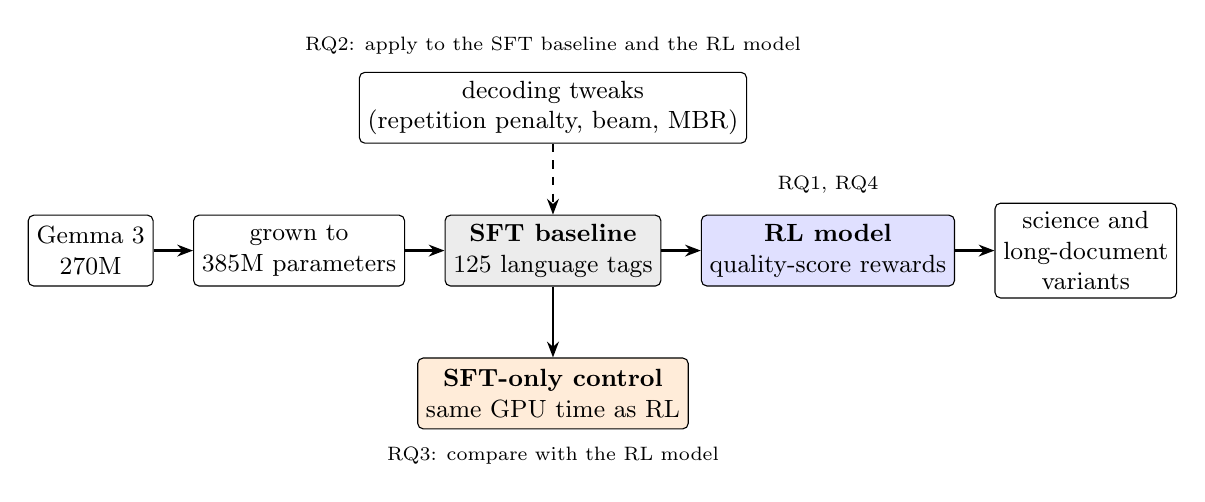
\begin{tikzpicture}[font=\small, node distance=5mm, box/.style={draw, rounded corners=2pt, align=center, minimum height=9mm, inner sep=3pt}, arr/.style={-{Stealth[length=2mm]}, thick}, lab/.style={font=\scriptsize, align=center}]
\node[box] (g) {Gemma 3\\ 270M};
\node[box, right=of g] (grow) {grown to\\ 385M parameters};
\node[box, right=of grow, fill=gray!15] (sft) {\textbf{SFT baseline}\\ 125 language tags};
\node[box, right=of sft, fill=blue!12] (rl) {\textbf{RL model}\\ quality-score rewards};
\node[box, right=of rl] (sci) {science and\\ long-document\\ variants};
\node[box, below=9mm of sft, fill=orange!15] (ctl) {\textbf{SFT-only control}\\ same GPU time as RL};
\node[box, above=9mm of sft] (dec) {decoding tweaks\\ (repetition penalty, beam, MBR)};
\draw[arr] (g) -- (grow); \draw[arr] (grow) -- (sft); \draw[arr] (sft) -- (rl); \draw[arr] (rl) -- (sci);
\draw[arr] (sft) -- (ctl); \draw[arr, dashed] (dec) -- (sft);
\node[lab, below=1mm of ctl] {RQ3: compare with the RL model};
\node[lab, above=1mm of dec] {RQ2: apply to the SFT baseline and the RL model};
\node[lab, above=1.5mm of rl] {RQ1, RQ4};
\end{tikzpicture}
\caption{Overview. A 270M model is grown to 385M parameters and fine-tuned (the SFT baseline), then trained with reinforcement learning (the RL model). Two controls ask what else could give the same gain: decoding changes (RQ2) and more fine-tuning for the same GPU time (RQ3).}\label{fig:overview}
\end{figure*}

\textbf{Model.} We start from Gemma-3-270m-it \citep{gemmateam2025gemma3} and add layers to reach 385M parameters (39 layers) \citep[cf.][]{wu2024llamapro,kim2023solar}. The task is English to one of 125 languages. A single extra token in the vocabulary names the target language, and the model answers with that token followed by the translation.

\textbf{Step 1: supervised fine-tuning (the SFT baseline).} We train on English-to-African sentence pairs and instruction data. Before training, we remove every pair that matches the text of any benchmark we later use, checked on both sides of the pair. Part of the data comes from NLLB-mined sentences and a collection of translated instructions; we report their share and licences in the Ethical considerations. Training uses the Muon optimiser \citep{liu2025muon} and takes about 45 hours on one A100 GPU (Appendix~\ref{app:hyper}).

\textbf{Step 2: reinforcement learning (the RL model).} We use GRPO \citep{shao2024deepseekmath}. For each English text the model samples 16 translations. Each translation receives a reward, and the model is nudged towards translations that score above the average of their group and away from those below it; a penalty keeps the model close to its starting point. Three stages follow one another, and the first does most of the work (Section~\ref{sec:rq4}). The reward has three parts. (i) A translation that fails a hard check scores the minimum: wrong or missing language tag, no end of text, a copy of the input, repetition, the wrong language, or an implausible length. (ii) Otherwise a quality score without a reference translation rates the output. We combine two quality models \citep{wang2024africomet,li2025ssacomet}, taking their mean unless they disagree strongly, and for languages without a validated quality model we reward agreement with the group's other samples. (iii) Small penalties discourage, among other things, unusual length, missing numbers or names, and missing diacritics. Exact settings are in Appendix~\ref{app:hyper}.

\textbf{Variants.} The \emph{SFT-only control} continues SFT from the baseline for the same GPU time as the RL stages, using half replay data and half extra English-to-X pairs for 19 languages \citep{gritta2026translatepsy}. The \emph{science variant} adds a short fine-tuning step on science text from AfriScience-MT \citep{abdulmumin2026afriscience} and then a second RL run; the \emph{long-document variant} adds RL on long inputs. Internal names used in the appendix tables are listed in Appendix~\ref{app:glossary}.

\section{Experimental Setup}\label{sec:eval}
% [M11 CT1-CT6 X1 X2 X5 X7 X9]
\textbf{Benchmarks.} We translate English into African languages on the standard FLORES+ devtest set \citep{oldi2025floresplus} (1,012 sentences; 54 languages), NTREX-128 \citep{federmann2022ntrex} (24 languages) and MAFAND-MT \citep{adelani2022mafand} (15 languages). Smaller sets, SmolSent \citep{caswell2025smol}, SALT \citep{akera2022salt}, GlotStoryBook \citep{kargaran2023glotlid}, IbomMT \citep{kalejaiye2025ibom} and FLORES-MOZ \citep{moznlp2026floresmoz}, appear in the appendix, as does AfriScience-MT \citep{abdulmumin2026afriscience} for science text. Unless stated, we report the average over languages, with each language counting equally.

\textbf{Metrics.} \emph{chrF++} compares character and word n-grams of the output with a human reference; higher is better. \emph{Held-out AfriCOMET} is a learned score that compares source, output and reference; we never use it as a reward. The \emph{finished rate} is the share of outputs that end properly; the \emph{loop rate} is the share that repeat themselves. Both are the checks our reward also uses, so they are not independent evidence of better translation. We computed chrF++ with sacreBLEU 2.6.0 (word order 2, otherwise defaults) after Unicode normalisation; the full signature string was not saved.

\textbf{Avoiding self-deception.} First, \emph{independence}: the metrics inside the reward (the two quality models, agreement between samples, and the finished, repetition and language checks) are not evidence that RL helped. Our evidence is chrF++ and held-out AfriCOMET against human references (Appendix~\ref{app:indep}). Second, \emph{paired tests}: every difference is a paired bootstrap over test sentences with a 95\% interval, which covers sentence variance but not training randomness. Third, \emph{contamination}: besides filtering the training pairs, we scanned 26 million training samples against all benchmark text and found no benchmark sentence of three or more words (Ethical considerations list the residuals). Fourth, \emph{seeds}: every model is one training run; we measured seed noise only for the first RL stage on 20 languages.

\textbf{Decoding.} All main results use greedy decoding with up to 768 new tokens (vLLM, bf16). The \emph{repetition penalty} used as a control is a decoding setting that discourages repeated tokens; we chose its strength on a development set by a rule fixed in advance. Beam search and MBR decoding are described where they appear.

\section{Results}\label{sec:results}

\subsection{RL against SFT, and what a decode-time guard recovers}\label{sec:rlsft}
% [R1 R2 R3 R4 R5 R6 R13 D5; EVID tables 1-2; E01] GATE E-01
``SFT'' is the 385M SFT final; ``RL'' is the final general RL model (mixed-stage best); 214 rows flagged by the contamination audit are removed. RL improves \chrfpp{} on every benchmark (Table~\ref{tab:headline}); plain chrF over the 93 cells improves by $+8.59$ \ci{+8.43}{+8.76} and held-out AfriCOMET (76 cells) by $+0.0631$ \ci{+0.0620}{+0.0643}. All 54 FLORES+ and 24 NTREX languages improve on \chrfpp{}, chrF and AfriCOMET with intervals above zero; on MAFAND-MT 14 of 15 improve (pcm $-0.25$ \ci{-0.69}{+0.30}).

\begin{table}[t]
\centering\footnotesize\setlength{\tabcolsep}{2pt}
\caption{RL against SFT (language-macro \chrfpp{}, clean rows, 95\% paired bootstrap, one seed).}\label{tab:headline}
\begin{tabular}{@{}lrrl@{}}
\toprule
benchmark (n) & SFT & RL & RL $-$ SFT\\
\midrule
FLORES+ (54) & 22.85 & 31.66 & $+8.81$ \ci{+8.59}{+9.03}\\
NTREX (24) & 29.25 & 37.17 & $+7.91$ \ci{+7.69}{+8.12}\\
MAFAND-MT (15) & 35.77 & 40.78 & $+5.01$ \ci{+4.76}{+5.23}\\
all 93 cells & 26.59 & 34.55 & $+7.96$ \ci{+7.82}{+8.12}\\
\bottomrule
\end{tabular}
\end{table}

\textbf{Finishing and looping.} On FLORES+ (finished / loop / hypothesis-to-reference length) the SFT has 0.829 / 0.209 / 3.03, RL stage A 0.983 / 0.068 / 1.33 and the mixed best 0.995 / 0.048 / 1.14 (Appendix~\ref{app:rlsft}). Cutting the SFT's looping outputs at the loop onset, without changing the translation, lifts the SFT from 26.59 to 30.49 \chrfpp{}: \textbf{49\% of the gain is recovered by cutting loops}. 67 to 70\% of the gain sits in rows where either model failed, and about 41\% of the AfriCOMET gain is finishing. On rows where the SFT finished and did not loop, RL is still $+2.41$ \ci{+2.33}{+2.49} \chrfpp{} and $+0.0366$ AfriCOMET ahead, significant in 50 of 54 FLORES+ languages; the estimates favour different models and agree in sign and rough size.

\textbf{Decode-time loop guard (E-01).} Greedy decoding with a vLLM frequency penalty of 0.10 (best of a seven-setting dev grid; plain greedy 34.50, best 37.36 dev \chrfpp{}) gives SFT $26.59\to30.48$ and RL $34.55\to34.84$ \chrfpp{} over the 93 cells, and AfriCOMET (76 cells) SFT $0.565\to0.583$, RL $0.628\to0.631$ (Figure~\ref{fig:decomp}). \textbf{A guard on the SFT recovers the same 49\% of the \chrfpp{} gain (29\% of the AfriCOMET gain) without RL}; RL with the guard minus SFT with the guard is $+4.37$ \ci{+4.28}{+4.46} \chrfpp{} and $+0.0479$ \ci{+0.0469}{+0.0490} AfriCOMET ($+2.63$ \ci{+2.56}{+2.70} \chrfpp{} on rows where the guarded SFT is clean). Caveats: the optimum (0.10) lies at the edge of the grid, so the control may be under-tuned; a post-hoc dev-only extension was still rising (SFT dev \chrfpp{} 37.36 at 0.10, 37.97 at 0.20, 38.00 at 0.30, 38.25 at 0.50) and no full evaluation with a stronger penalty was run; one seed. With the guard, FLORES+ zgh and MAFAND-MT pcm are significantly worse for RL than for the SFT.

\begin{figure*}[t]
\centering
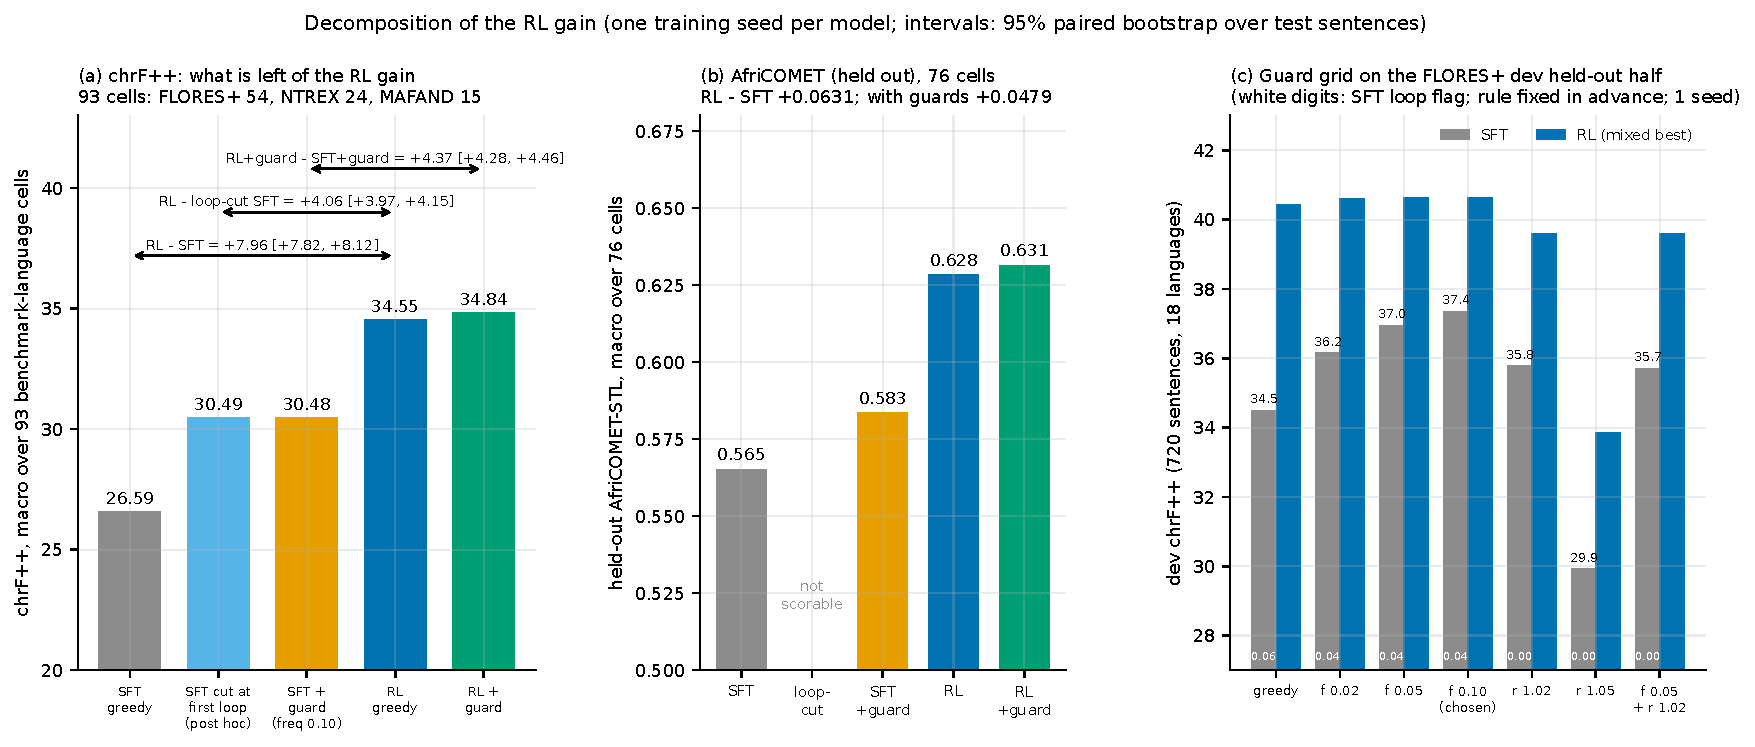
\includegraphics[width=\textwidth]{figures/fig3_decomposition_guard.pdf}
\caption{Decomposition of the RL gain with the decode-time guard (E-01). (a) Language-macro \chrfpp{} over 93 cells: SFT 26.59, SFT cut at its first loop 30.49 (post hoc), SFT with frequency penalty 0.10 30.48, RL 34.55, RL with guard 34.84; arrows give paired differences with 95\% CI. (b) Held-out AfriCOMET over 76 cells. (c) The seven-setting guard grid on the FLORES+ dev held-out half (720 sentences, 18 languages); the optimum (0.10) lies at the edge of the grid. One seed per model.}\label{fig:decomp}
\end{figure*}

\textbf{Growth and the earlier model.} The 385M SFT is significantly better than A0 on seven of eight benchmarks (FLORES+ $+5.31$ \ci{+5.13}{+5.50}, 46 languages; the comparison confounds depth with the extra stage-B SFT). In the same harness, on rows clean for both generations (E-13), it is behind our earlier 270M SFT on FLORES+ ($-2.35$ \ci{-3.25}{-1.38}), NTREX ($-4.13$) and MAFAND-MT ($-3.54$); after RL it is level on FLORES+ ($+0.35$ \ci{+0.08}{+0.62}) and NTREX ($+0.02$ \ci{-0.07}{+0.11}) and $1.55$ \chrfpp{} lower on MAFAND-MT, with data, steps, tokenizer layout and reward differing and only 4.7\% of FLORES+ rows kept (Appendix~\ref{app:sft}).

\subsection{Independent audit of the loop flag}\label{sec:degen}
% [R19-R24 DEGEN]
The reward's loop flag is the guard the RL was optimised against, so a missed loop type would be undercounted for RL. We re-measured with a detector sharing the idea but none of the code or constants (lzma-compressed size relative to human references of the same benchmark, language and length; repeated character 8-grams; repeated word 3-grams; each threshold set so that 0.1\% of 122,585 human references fire it). \textbf{The reward's flag is a lower bound:} on mixed-best FLORES+ the independent detector flags 1.77 \ci{1.71}{1.84} times as many outputs (0.0851 against 0.0480; SFT 0.3107 against 0.2095, ratio 1.48). The extra rows are finished partial repetitions: if they scored the average of their language's unflagged rows, mixed-best macro \chrfpp{} would rise by at most 0.19 (FLORES+), against 0.46 for the SFT, so the decomposition changes by 3.0\% to 4.4\% of the RL gains at most. Two further findings: 24.5\% of the 2,079 mixed-best rows above twice the reference length are flagged by neither detector, and \textbf{English output rises in the Arabic dialects and Tamazight} (aeb 0.215 to 0.449, ary 0.041 to 0.394, arz 0.006 to 0.098, zgh 0.001 to 0.049, SFT to mixed best; languages outside the RL prompt pool), so part of ``RL loops less'' there is a change from loops to English, while their \chrfpp{} stays at 2 to 9 (Appendix~\ref{app:degenapp}).

\begin{figure*}[t]
\centering
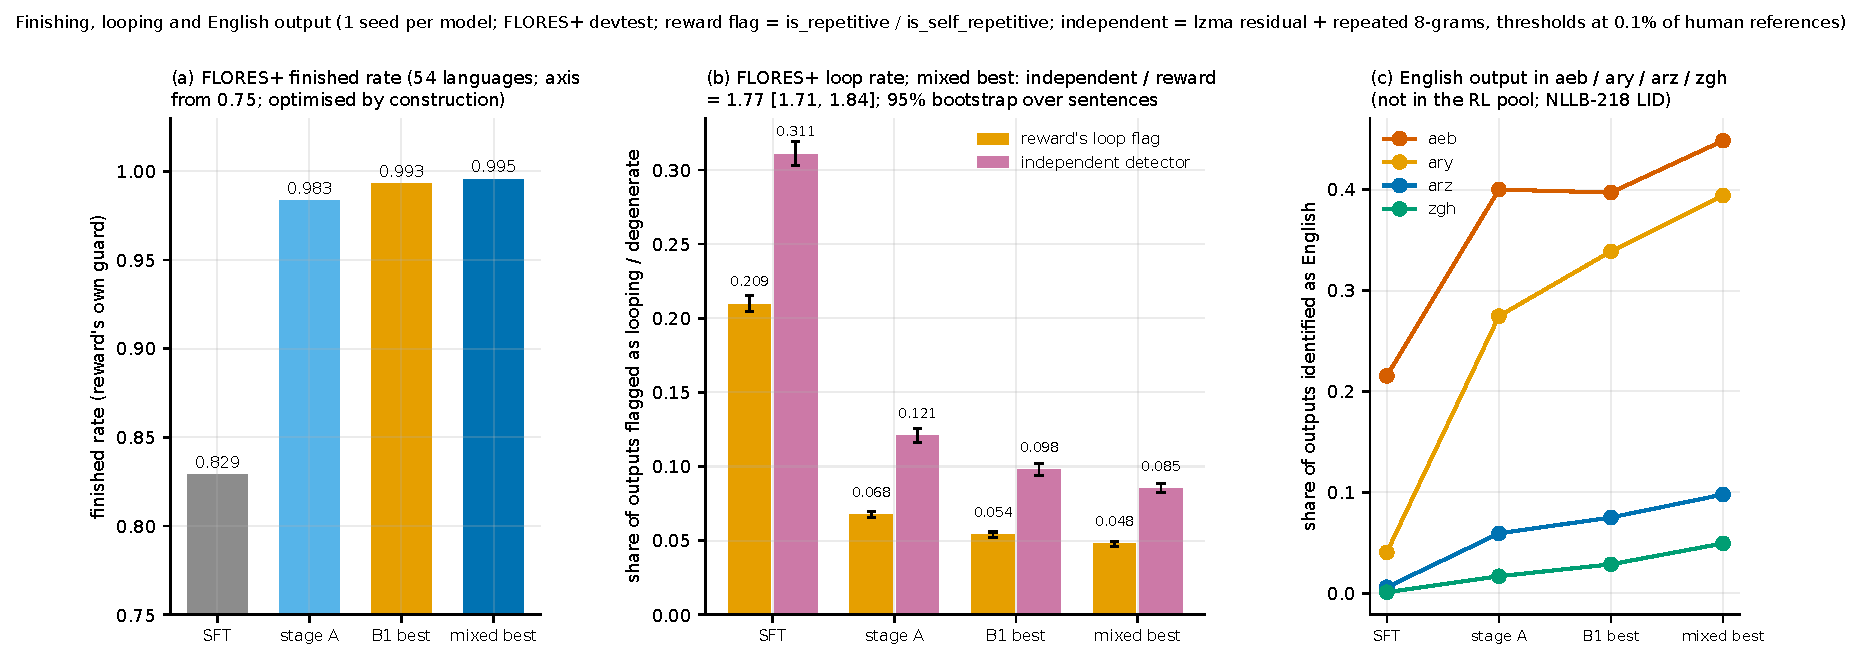
\includegraphics[width=\textwidth]{figures/fig7_loops_finishing.pdf}
\caption{Finishing, looping and English output on FLORES+ devtest (language macro, one seed per model). (a) Finished rate (54 languages; axis from 0.75). (b) Reward loop flag against the independent detector; error bars 95\% bootstrap over source sentences. (c) Share of outputs identified as English (NLLB-218 LID, $p\ge0.5$) in four languages outside the RL prompt pool.}\label{fig:loops}
\end{figure*}

\subsection{Where the gain accrues; seeds and ablations}\label{sec:seeds}
% [R8 E04 E11 M10 R17 R18]
Stage A gives 94\% of the SFT-to-B1 gain on FLORES+ (7.96 of 8.50); B1 adds $+0.54$ \ci{+0.49}{+0.59} and the mixed stage $+0.31$ \ci{+0.26}{+0.35} (NTREX $+0.30$, $+0.18$; MAFAND-MT nothing). B1 final (step 135) equals B1 best within noise. \textbf{Seeds (E-04).} Two extra runs of the stage-A recipe (100 steps, 20 languages, 49 cells) gain $+5.96$ \ci{+5.80}{+6.11} and $+5.90$ \ci{+5.74}{+6.05} \chrfpp{} over the SFT; they differ by \textbf{0.06} \ci{-0.02}{+0.14}. On those languages B1 best is $+0.17$ \ci{+0.12}{+0.21} over stage A, about three times the seed difference, while the mixed step is $+0.07$ \ci{+0.02}{+0.11}, the size of the seed difference: \textbf{we do not call the mixed step a gain}. This is one pair of seeds at step 100, not a seed study of later stages. RL aimed at eight weak West-African languages (85 steps, MBR guide) adds $+0.03$ \ci{-0.06}{+0.12} on its targets against a pre-registered $+1.0$ (negative result).

\textbf{Ablations (E-11).} One run per arm, 100 steps, forks of seed 2's step-40 state (Figure~\ref{fig:seeds}). Removing all four stage-A features costs \textbf{0.32} \ci{0.23}{0.41} \chrfpp{} (about 5\% of the gain, five times the seed difference); removing the reference domain costs 0.16 \ci{0.08}{0.25}; removing the beam guide costs 0.09 against seed 2 but $0.04$ \ci{-0.04}{+0.11} against seed 3, \textbf{not separable from seed noise}, for 25\% more step time. The KL rise is not caused by the features (median KL of steps 81 to 90: 0.116 without any feature, 0.120 to 0.123 in the other arms). The features are design choices with a small measured benefit.

\begin{figure*}[t]
\centering
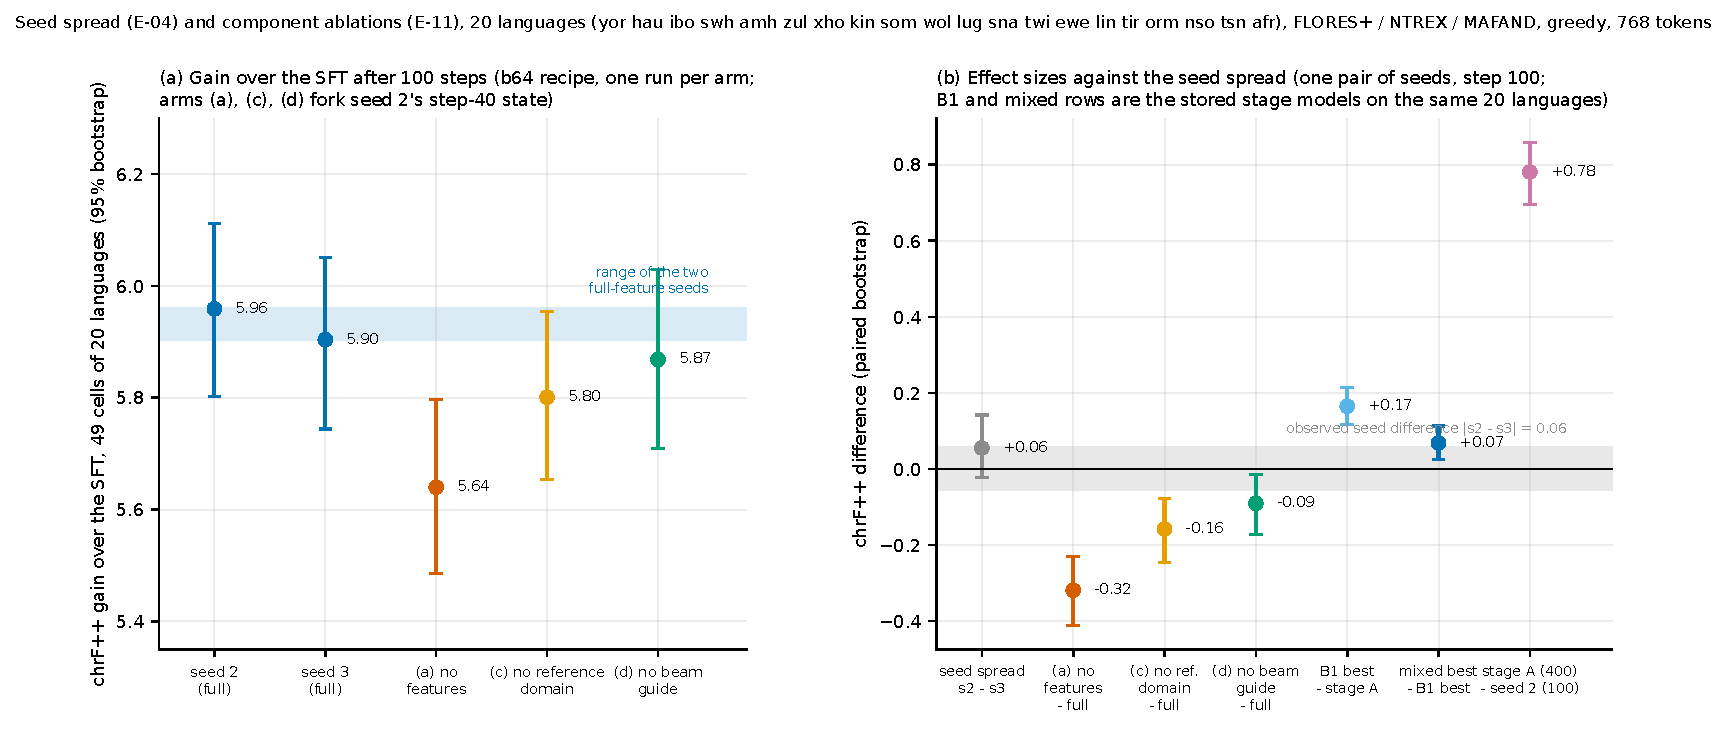
\includegraphics[width=\textwidth]{figures/fig16_e04_e11_seeds_ablations.pdf}
\caption{Seed spread (E-04) and ablation arms (E-11), 20 languages, 49 cells, greedy, 768 tokens, 95\% paired bootstrap. (a) \chrfpp{} gain over the SFT after 100 steps for two full-feature seeds and three ablation arms (shaded: range of the two seeds). (b) Effect sizes against the observed seed difference $|s_2-s_3|=0.06$: ablation arms minus seed 2, the B1 and mixed steps on the same languages, and the 400-step stage A minus seed 2. One pair of seeds, step 100.}\label{fig:seeds}
\end{figure*}

\subsection{Beam search and MBR (E-02)}\label{sec:decoding}
% [D1-D7 E02]
On 4,000 sentences (20 languages $\times$ 200 FLORES+ sentences) at 768 tokens, vLLM's beam search lets a runaway continuation beat every ended hypothesis, so the primary beam-4 (amended before any score) stops when 4 hypotheses have ended; a Hugging Face-style rule (\texttt{early\_stopping=False}) is a second beam. MBR-16 uses 16 samples plus the greedy output with \chrfpp{} as utility (metric-matched). Decoders help the SFT (beam-4 $+3.71$ \ci{+2.78}{+4.47}, MBR-16 $+5.96$ \ci{+5.37}{+6.49} \chrfpp{}); for the RL model MBR-16 adds $+0.92$ \ci{+0.81}{+1.03}, beam-4 (stop at 4) $-0.77$ \ci{-1.45}{-0.25} and the HF-rule beam $+0.83$ \ci{+0.67}{+1.00}: the sign of the RL beam result depends on the stopping rule. \textbf{Decoding does not replace RL}: RL greedy is $+1.60$ \ci{+1.34}{+1.88} \chrfpp{} ahead of the best decoded SFT (MBR-16, about 17 times the compute). RL minus SFT shrinks from $+7.56$ (greedy) to $+3.07$ (beam-4) and $+2.52$ (MBR-16): the RL gain is partly the same repair. Caveats: 20 languages, one checkpoint each; the beam numbers of an earlier 256-token study are not comparable (Appendix~\ref{app:decoding}). \textbf{Precision (E-09b):} bf16 and fp32 outputs differ between engines, but the SFT in fp32 on the full set scores $-0.04$ \ci{-0.13}{+0.07} \chrfpp{} against bf16 over the 93 cells, and the RL gain on FLORES+ is $+8.97$ \ci{+8.71}{+9.20} over the fp32 SFT against $+8.81$ over the bf16 SFT, so the bf16 harness does not overstate it; the RL model was not run in fp32.

\begin{table*}[t]
\centering\small\setlength{\tabcolsep}{3pt}
\caption{\chrfpp{} at 768 new tokens, language macro over 20 languages, 4,000 sentences per row, 95\% paired bootstrap (E-02).}\label{tab:e02}
\begin{tabular}{@{}lll@{}}
\toprule
decoding & SFT & RL (mixed best)\\
\midrule
greedy & 32.31 \ci{31.43}{33.38} & 39.87 \ci{39.17}{40.62}\\
beam-4, stop at 4 ended & 36.02 \ci{35.13}{36.95} & 39.10 \ci{38.20}{39.96}\\
beam-4, HF rule & 33.26 \ci{32.22}{34.46} & 40.70 \ci{40.00}{41.42}\\
MBR-16 & 38.27 \ci{37.60}{39.01} & 40.79 \ci{40.09}{41.54}\\
\bottomrule
\end{tabular}
\end{table*}

\subsection{Matched-compute continued-SFT control (E-03)}\label{sec:control}
% [R14 CTL7-CTL11] reports/e03_sft_control_2026-11-05.md; GATE E-03
To ask whether the GPU time of the RL chain (8.66 \GPUh{}) would do as well as more SFT, we continued the SFT final for 6,000 steps (8.4 h) at a constant learning rate of $10^{-5}$ (chosen by a probe fixed in advance), with 16 replay packs and 16 packs of TranslatePsy English-to-X pairs \citep{gritta2026translatepsy} per step: NLLB-3.3B translations of MADLAD-400 sentences for 19 languages, 277,900 pairs each, scanned against the protected index and used once. The decision rule, primary endpoint (language-macro \chrfpp{} over 93 cells, RL minus control) and language panels were written down before any benchmark of the control was looked at. \textbf{Only the 6,000-step checkpoint was evaluated}; the stage-A-matched (3,100) and mixed-best-matched (4,800) checkpoints exist but were not evaluated.

\begin{table}[t]
\centering\footnotesize\setlength{\tabcolsep}{3pt}
\caption{Continued-SFT control against the RL mixed best; language-macro \chrfpp{}, clean rows, 95\% paired bootstrap; TP = the 19 TranslatePsy languages. Held-out AfriCOMET, RL $-$ control: $+0.0183$ (all), $-0.0249$ (TP), $+0.0883$ (other).}\label{tab:e03}
\begin{tabular}{@{}lccl@{}}
\toprule
cells & control & RL & RL $-$ control\\
\midrule
all (93) & 29.97 & 34.55 & $+4.58$ \ci{+4.45}{+4.70}\\
TP (47) & 41.37 & 41.34 & $-0.03$ \ci{-0.13}{+0.09}\\
other (46) & 18.32 & 27.61 & $+9.29$ \ci{+9.09}{+9.49}\\
\bottomrule
\end{tabular}
\end{table}

The registered rule had four conditions: lower bound of the overall difference above $+1.0$ (met: $+4.58$ \ci{+4.45}{+4.70}), AfriCOMET lower bound above 0 (met: $+0.0183$ \ci{+0.0172}{+0.0192}), difference above 0 on the other languages (met) and difference above 0 on the 19 TranslatePsy languages (\textbf{not met}: $-0.03$). \textbf{By the rule as registered the verdict is ``inconclusive''}, and we did not change the rule. Reading the panels: where a teacher-translated corpus exists, continued SFT matches RL in \chrfpp{}, largely fixes finishing and looping (FLORES+ finished 0.993 against 1.000 for RL), and is ahead on the neural metrics; on the other languages it changes almost nothing ($+0.15$ \chrfpp{} over the SFT on FLORES+, \ci{-0.03}{+0.32}), while RL improves them all from its own samples ($+9.29$). The overall endpoint alone reads ``RL is better'', the 19 languages alone ``comparable''; neither is the registered verdict. Caveats: one seed, one learning rate, one budget point; the control is not information-matched (NLLB-3.3B scores 38.80 against 26.30 for the SFT on 43 languages), and the TranslatePsy rows were filtered with AfriCOMET, SSA-COMET and MetricX, so those neural metrics favour the control; chrF and \chrfpp{} are the evidence.

\begin{figure*}[t]
\centering
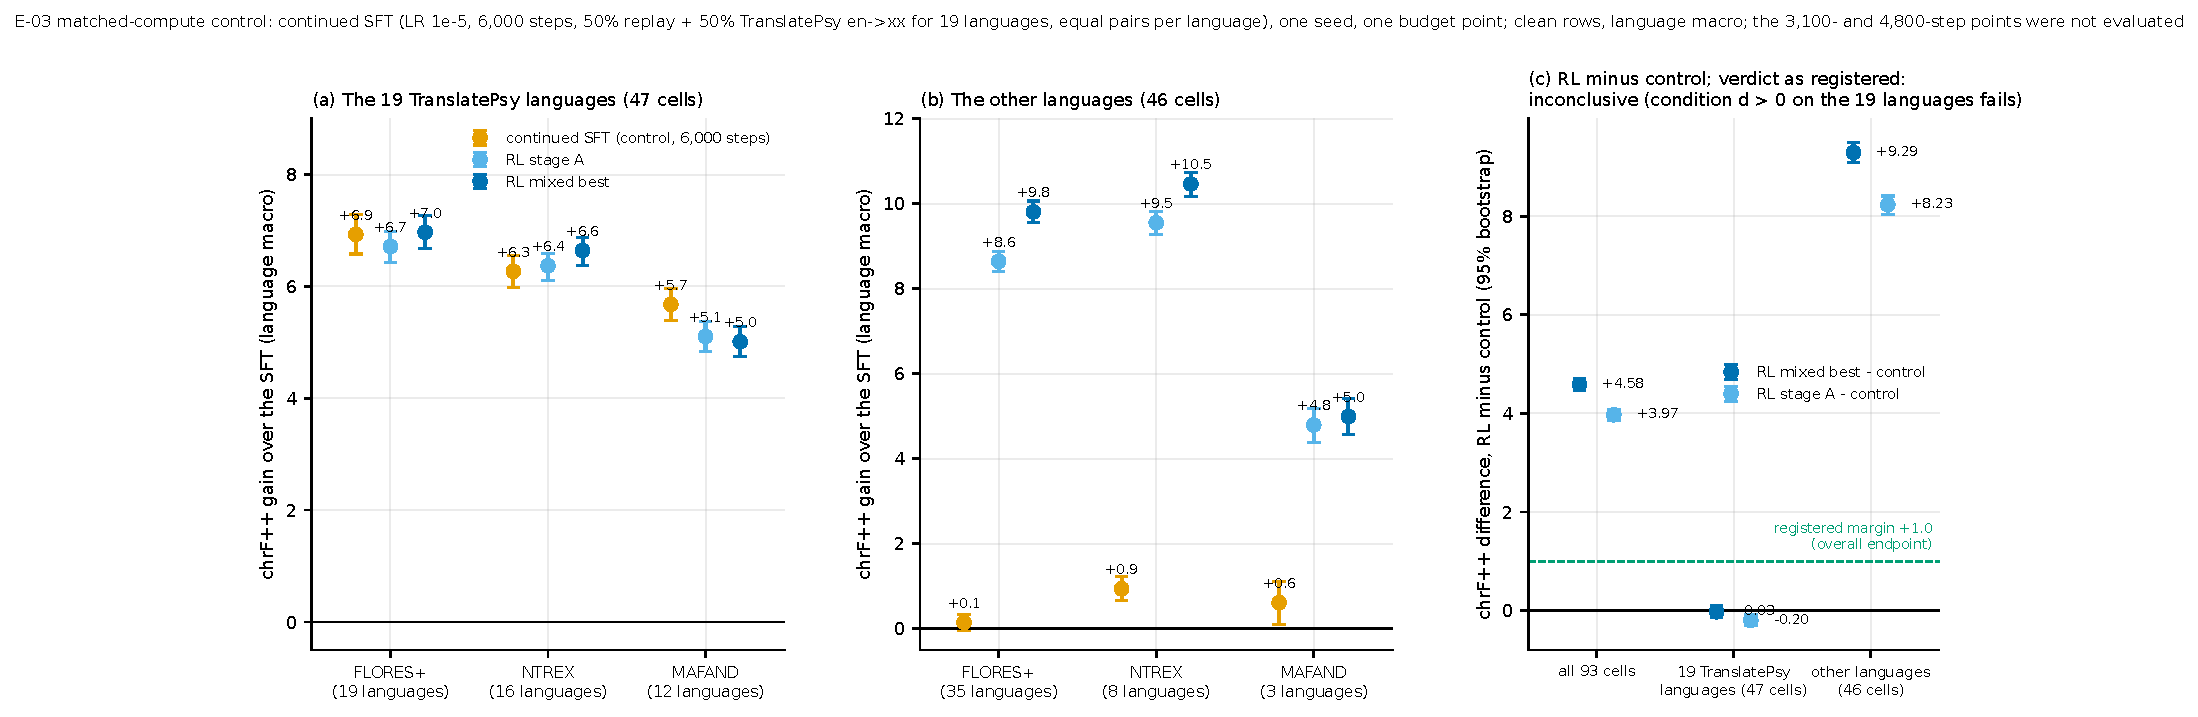
\includegraphics[width=\textwidth]{figures/fig14_e03_control.pdf}
\caption{Matched-compute continued-SFT control (E-03). (a, b) \chrfpp{} gain over the SFT (language macro, 95\% bootstrap) of the control, RL stage A and RL mixed best by benchmark, for the 47 cells of the 19 TranslatePsy languages (a) and the 46 other cells (b). (c) RL minus control for all 93 cells and for the two panels, with the registered $+1.0$ margin; the registered verdict is inconclusive. One seed per model; only the 6,000-step checkpoint was evaluated.}\label{fig:e03}
\end{figure*}

\subsection{Comparison with NLLB-200}\label{sec:nllb}
% [N1-N6 NLLBRL]
NLLB-200 3.3B (the 3.3B variant of its model card) has about 8.6 times the parameters of our 385M model. On the 43 languages shared with the published FLORES-200 devtest table, the mixed best reaches 35.54 \chrfpp{} against 38.80 for NLLB-3.3B ($-3.26$, language-bootstrap \ci{-4.29}{-2.20}; 92\%; SFT 26.30, $-12.50$, 68\%): RL closes 74\% of the gap, and the remaining gap is not a finishing artefact (the mixed best finishes at least 0.99 in every language). It matches or beats NLLB-3.3B on 7 of 43 languages, all in the lowest tertile (e.g. yor $+5.43$, fon $+2.95$); the largest gaps are amh $-11.28$, kin $-9.74$, kea $-8.72$. Caveats: FLORES-200 against FLORES+ references, NLLB beam against our greedy (beam and MBR move our \chrfpp{} by $-0.77$ to $+0.92$), the 11 hardest languages have no NLLB row, five of the 43 languages had an NLLB pseudo-reference reward term, the yor value is anomalously low, intervals are over languages, one seed. We state only that, size-aware, the model reaches 92\% of NLLB-3.3B's \chrfpp{} on these languages and matches or beats it on 7 of 43; we do not claim to beat NLLB or to be competitive with it overall.

\begin{figure*}[t]
\centering
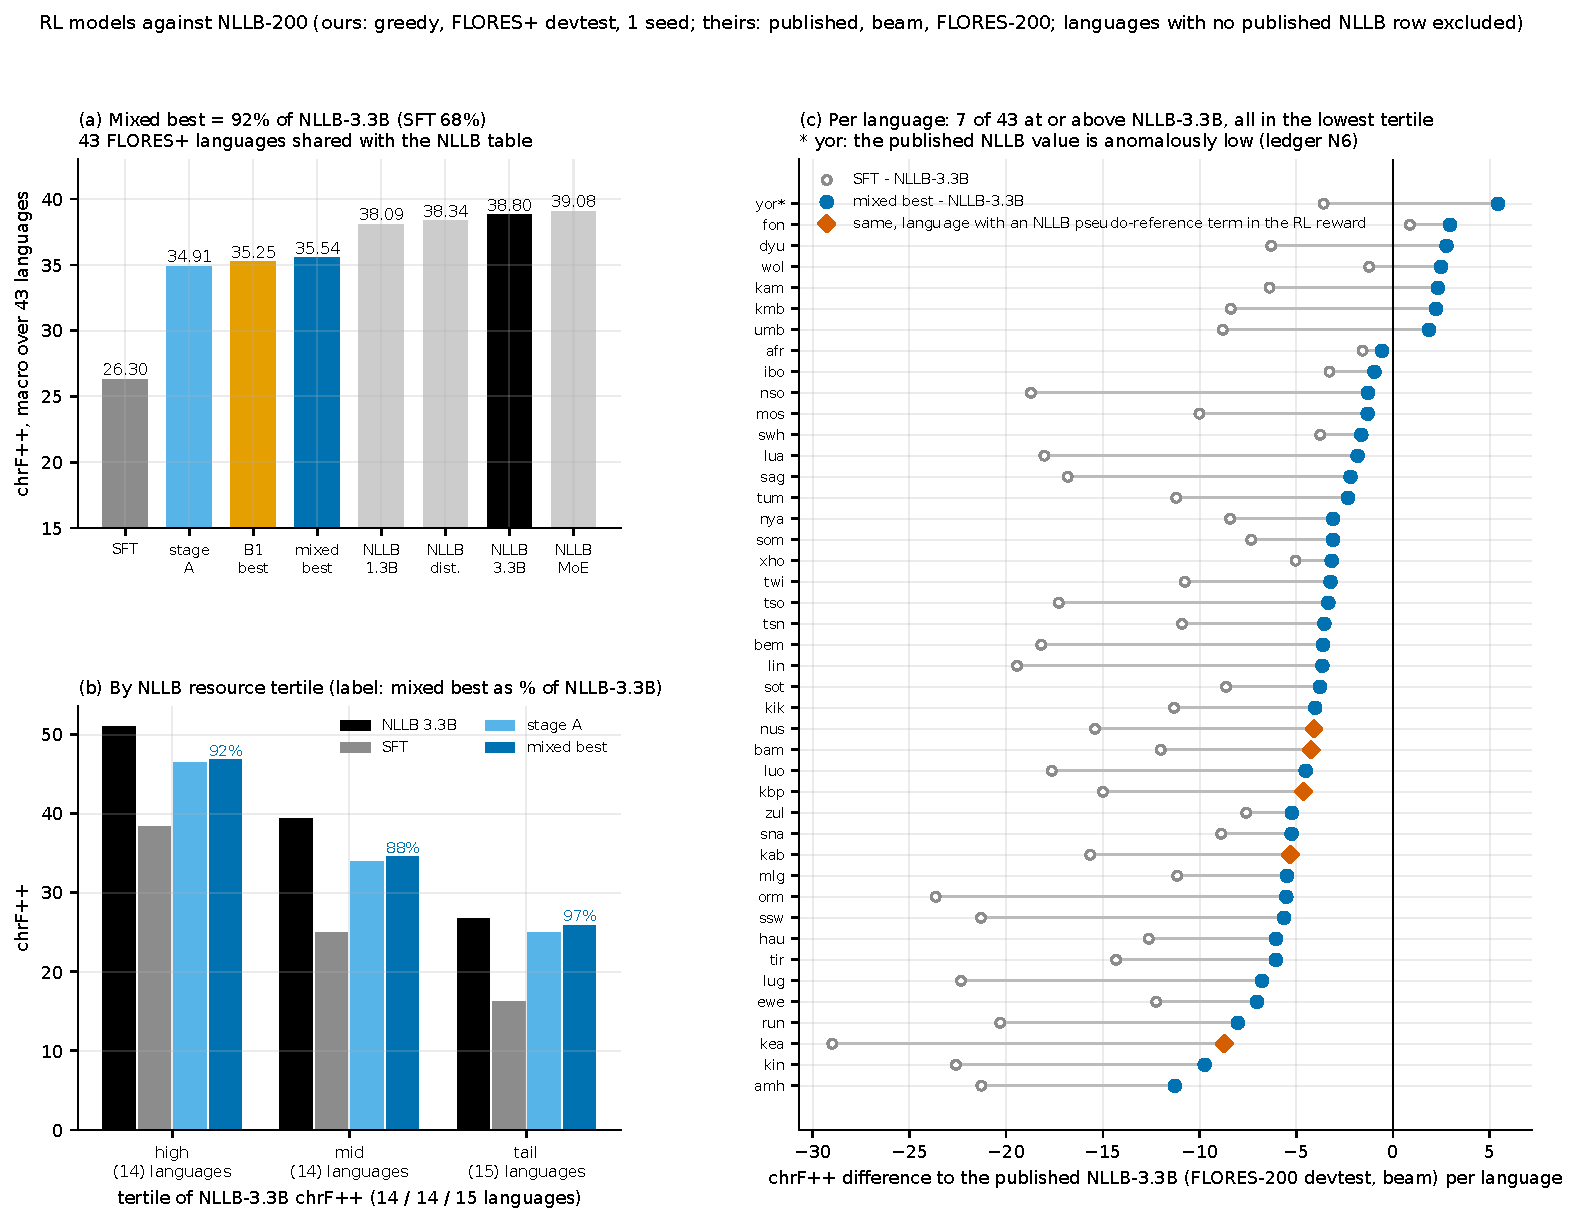
\includegraphics[width=0.62\textwidth]{figures/fig4_nllb_43.pdf}
\caption{RL models against NLLB-200 on the 43 shared FLORES+ languages (ours: greedy, one seed per model; NLLB: published FLORES-200 devtest, beam). (a) Language-macro \chrfpp{}: mixed best 35.54 against NLLB-3.3B 38.80 (92\%; SFT 68\%). (b) By tertile of NLLB-3.3B \chrfpp{} (14/14/15 languages). (c) Per-language difference to NLLB-3.3B, SFT (open) and mixed best (filled); orange diamonds: languages with an NLLB-3.3B pseudo-reference reward term; yor$^*$: anomalously low published value. Intervals are over languages only.}\label{fig:nllb}
\end{figure*}

\subsection{Science and long-document RL}\label{sec:science}
% [SC1-SC6 DL1-DL5 P4 E05 E15 E16]
A science SFT with weight interpolation ($\alpha=0.5$) gives surface gains on AfriScience-MT (chrF $+1.2$) and no SSA-COMET-QE gain (0.6130 to 0.6118). A science RL adds $+0.46$ chrF \ci{+0.27}{+0.65} and $+0.0053$ AfriCOMET on test sentences over its start, and nothing at document level. \textbf{The science SFT, not the science RL, carries the science gain (E-14):} the same RL started from the mixed best, without the science SFT, ends $-1.44$ chrF \ci{-1.61}{-1.25} and $-0.0082$ AfriCOMET \ci{-0.0101}{-0.0065} below the executed science RL and adds only $+0.26$ chrF \ci{+0.12}{+0.39} over its start, so by the registered rule the science SFT is needed; SSA-COMET-QE rates it level ($-0.0006$ \ci{-0.0018}{+0.0007}), a reward-family effect rather than evidence of quality. One seed, one out-of-memory restart, final checkpoint only (Appendix~\ref{app:docs}). Whole-document generation (4,096 tokens) fails for the 385M models; a long-document RL raises whole-document finishing from 0.70 to 0.82 ($+0.125$ \ci{+0.046}{+0.204}) and lowers the loop rate from 0.85 to 0.73, but 72 to 73\% of documents still loop and chunked decoding is required; the earlier 270M model is as good or better at document level. Table~\ref{tab:sci} gives sentence-level scores for every stage (SSA-COMET-QE is of the reward family; the first RL stage adds $+0.043$ and later stages at most $+0.005$ more, while chrF and AfriCOMET keep rising slightly).

\begin{table}[t]
\centering\footnotesize\setlength{\tabcolsep}{3pt}
\caption{AfriScience-MT test, sentence level (970 sentences per language; macro over amh hau lug nso yor zul; greedy; one seed per stage). SSA-QE = SSA-COMET-QE, of the reward family for every RL row.}\label{tab:sci}
\begin{tabular}{@{}lccc@{}}
\toprule
stage & chrF & AfriCOMET & SSA-QE\\
\midrule
SFT & 36.00 & 0.6064 & 0.5686\\
RL stage A & 45.06 & 0.6822 & 0.6118\\
RL mixed best & 45.40 & 0.6828 & 0.6130\\
science RL w/o SFT (E-14) & 45.66 & 0.6850 & 0.6153\\
science SFT ($\alpha=0.5$) & 46.63 & 0.6879 & 0.6118\\
science RL final & 47.10 & 0.6932 & 0.6158\\
long-document RL final & 47.16 & 0.6936 & 0.6165\\
\bottomrule
\end{tabular}
\end{table}

\section{Discussion and Conclusion}\label{sec:discussion}
% [paper.md 12.1-12.3; GATE E-01 E-03]
Under automatic metrics, RL with reference-free QE rewards beats the SFT everywhere, but about half of the \chrfpp{} gain (49\%; 29\% of the AfriCOMET gain) is finishing and looping that a one-line decode-time guard also removes, and beam/MBR decoding repairs a further part. What RL adds beyond a guarded SFT is $+4.37$ \chrfpp{}; nearly all of it arrives in the first stage, and the mixed step is not separable from seed noise. Our reading, only partly tested, is that the SFT's main defect is unguarded greedy decoding and that the hard-failure floor and the QE reward teach the policy to avoid it within about a hundred steps. Against continued SFT for the same GPU time the registered verdict is ``inconclusive'': the control matches RL on the 19 languages it has teacher data for and does nothing for the other 46 cells, so what RL contributes, in our data, is breadth. We do not claim that the \chrfpp{} beyond finishing is quality a human would confirm, that any reward component other than the stage-A features helped, or that the model is usable for Arabic dialects, Tamazight, Dinka, Tamasheq or Kanuri. In science translation the science SFT, not the science RL, carries the gain (E-14: the same RL without it ends $-1.44$ chrF \ci{-1.61}{-1.25} lower). Next experiments: stronger guards in full evaluation, the unevaluated control checkpoints, later-stage seeds and human judgement of outputs.

\FloatBarrier\label{coreend}
\clearpage
\section*{Limitations}
% [paper.md section 13; full list in the appendix of the full version]
\textbf{Automatic scoring only.} The references of FLORES+, NTREX-128 and MAFAND-MT are human translations, but all scoring is automatic: no human judgement of system outputs was collected. The neural scores belong to one family, and AfriCOMET has a length and entity bias.
\textbf{One training run per model.} We measured seed noise only for the first RL stage, on 20 languages and 100 steps, with one pair of extra seeds. The last RL step and per-language differences below about half a point cannot be separated from seed noise. A second seed of the SFT baseline is impractical (about 45 GPU-hours).
\textbf{The matched-compute control is one run:} one seed, one learning rate, one data mix with NLLB-3.3B targets and one evaluated stopping point. The repetition-penalty control chose its best value at the edge of the range searched.
\textbf{Rewarded metrics are not evidence.} The finished, repetition and language checks, and the quality scores the RL optimises, are part of the reward. The independent repetition detector shares the idea of the reward's check and cannot see non-repetitive failures.
\textbf{Ablations are limited:} three arms, 100 steps, one run each, 20 languages; later RL stages and most reward ingredients were not ablated, and mid-run changes (Ethical considerations) mean the stages are not one clean design.
\textbf{Decoding and engine.} Headline numbers use one inference engine in bf16. The two engines differ in bf16 but agree in fp32; we did not run the RL model in fp32. Beam search and MBR cover 20 languages and one beam width.
\textbf{Coverage and comparisons.} Fifty-one of the 125 languages have no reference test and are unscored. The model fails on Arabic dialects, Tamazight, Dinka, Tamasheq and Kanuri, where RL increases English output. Comparisons with the earlier 270M model and with NLLB mix differences in data, steps, test sets and decoding: our decoding is greedy, NLLB's is beam search, and on NTREX and MAFAND-MT only language-level NLLB averages exist (no sentence pairing, no AfriCOMET). Document results rest on 28 papers per language, and whole-document translation remains unusable.
\textbf{Not run.} Human judgement of outputs; the NLLB-data ablation; scans of packed training shards for contamination; a 54-language decoding study; a science fine-tuning step at full strength followed by RL; a second seed of the science run; long-document RL from the no-science-step model.

\section*{Ethical considerations}
% [DISCLOSURES sections 1-6; L1-L5 CT1-CT13 CTL1-CTL6; CFU]
\textbf{Data and licences.} NLLB-mined bitext (OPUS-NLLB, 43 languages; Fulah) is 14.4\% of the 3.990\,B stage-B pack tokens (10.84\% of the 5.043\,B tokens drawn in the whole SFT); with NLLB-Seed and the aligned part of Aya (NLLB-3.3B outputs) 18.7\%; with machine-translated Tumbuka instruction sets (system not stated, possibly NLLB) 22.8\%. NLLB models and outputs carry CC-BY-NC terms, which limits the commercial use of NLLB-derived data and signals, and a licence statement must accompany any release of the weights. Sources with unspecified or unconfirmed licences (the \texttt{*\_mt560} OPUS sets, 69\% of the main pair output, mostly Jehovah's Witnesses and Bible text; \texttt{multi-open}; AfroLingu-MT; an Efik New Testament sheet) need a legal decision, and religious text dominates many low-resource languages. IbomMT (CC-BY-NC-4.0) is a disclosed non-commercial exception. NLLB-3.3B pseudo-references (CC-BY-NC) are a reward signal for five languages, reward only. RL prompts (FineWeb-Edu, Wikipedia, news including BBC News with no declared licence and BBC copyright) are input text only. Gemma terms apply to the derived weights and its pretraining exposure cannot be excluded. Reward and monitor models, as declared on the Hub (read 2026-11-05): \texttt{ssa-comet-mtl}, \texttt{ssa-comet-qe} and the two AfriCOMET checkpoints apache-2.0; GlotLID \texttt{license: other} with \texttt{license\_name: apache-2.0-plus-notices} (Apache License 2.0 plus notices).

\textbf{Release and licence.} \anonreal{Checkpoints are anonymised for review and released on acceptance; the control checkpoint of E-03 is not released.}{The final RL model (branch \texttt{main}, the mixed best) is at \url{https://huggingface.co/AletheiaAING/gemma-0.4B-translate-rl}, the SFT model at \url{https://huggingface.co/AletheiaAING/gemma-0.4B-translate-sft} and the seed, ablation and E-14 weights at \url{https://huggingface.co/AletheiaAING/gemma-0.4B-translate-rl-experiments}; the control checkpoint of E-03 is not released.} At the last check the Hub repositories declare no licence field and have no model card; the Gemma terms of use apply to the derived weights, and the NLLB-derived and non-commercial data above limit commercial use \ownerdecision{confirm release licence}. The state, prompts, eval and reports repositories were private at the last check \ownerdecision{which parts of the data are released}.

\textbf{TranslatePsy.} \texttt{qvac/\allowbreak TranslatePsy-\allowbreak AfriSLM-\allowbreak Synthetic-\allowbreak Mix} (CC-BY-NC-4.0; targets are NLLB-3.3B translations of MADLAD-400 sentences filtered by AfriCOMET, SSA-COMET and MetricX) was used for the matched-compute control only. No TranslatePsy row is in the SFT, any RL stage, the science or long-document stages or any released weight; the control checkpoint is a research artefact that is neither released nor used in production. A good control result partly means ``distilling NLLB''. The NLLB-218 language-ID model (CC-BY-NC) was used for measurement only.

\textbf{Decontamination residuals (this pipeline, the clean 385M rerun).} The audit of the 385M training text finds no benchmark sentence of three or more words; benchmark rows that match are one- or two-word strings, numerals and names (NTREX 120 of 47,928 rows, 0.25\%; MAFAND-MT 94 of 20,009, 0.47\%; SmolSent 45 of 38,833; GlotStoryBook 15 of 3,426). The FLORES+ dev train half (440 ids) is in training on purpose and the held-out half is protected. A lexical fuzzy scan (56,975,939 pair rows, 4,277,612 instruction rows) finds no benchmark string of 8 or more tokens as a contiguous run, but strings of 4 to 7 tokens occur inside longer text (English side: MAFAND-MT 134 of 17,428, GlotStoryBook 30 of 898, NTREX 18 of 1,973, SALT 12 of 498) and 263 (string, benchmark) cases of 8+ token strings overlap training text by character 5-grams (candidates, effect on scores not measured). Stage A drew 6 flagged prompts of 28,120 (0.021\%) from seven unfiltered prompt files; 305 of 34,007 AfriScience-MT train rows (0.9\%) have their African-language sentence in the A0 pair data (test papers untouched). Embedding or MT-round-trip paraphrase scans and packed-shard scans were not run. Statements about the earlier 270M pipeline, whose training text held the English side of 95\% of FLORES+ devtest, do not apply to this rerun; its numbers appear only on rows clean for both generations.

\textbf{Analysis decisions and process.} Checkpoints were selected on a 720-sentence FLORES+ dev subset; the weak-language choice used devtest-derived per-language tables; the decomposition and family analyses were run after the results were known; the science headline metric changed after the interpolation rule was written. The RL preflight and stage-A gates failed and were overridden by the authors; stage A was stopped at step 40 and resumed with four features; B1 was restarted twice and the mixed stage once (the hacking alarm was loosened); the science-RL step cap was extended from 150 to 190 and the run stopped on a dev plateau after 160 steps; the long-document RL lost about 4.5 of 7.7 h to a crash loop, and the E-14 run had one out-of-memory restart (steps 21 to 38 replayed; the later records are used). LibreTexts rows were removed from the long-document pool before it started.

\textbf{Intended use, risks and dual use.} Outputs are machine translations of unverified quality for languages without human judgement, with documented failure modes (Arabic dialects, Tamazight, Dinka, Tamasheq and Kanuri are not usable; RL increases English output there; use sentence by sentence, not on whole documents). The model should not replace NLLB-class systems or be used where mistranslation is costly (health, legal, safety). As with any translation model it can be used to produce text at scale in under-served languages, including spam or misleading content, and we release no content-filtering component. Released artefacts are anonymised for review and released on acceptance.

\ifanon\else
\section*{Author contributions}
\textit{[Placeholder, to be filled by the lead author: one sentence per person describing what that person contributed (for example design, data, training, evaluation, writing). Authorship is based on contribution.]}
\fi
\bibliography{refs}
\bibliographystyle{acl_natbib}

\clearpage
\appendix
\label{appstart}
\onecolumn
% Appendix: generated from paper_385m/paper.md by a small converter, then kept as hand-editable LaTeX. Report keys and claim IDs are in % comments.

\FloatBarrier

\section{Hyper-parameters, recipe and reward details}\label{app:hyper}

This appendix collects the SFT and RL settings that Sections~\ref{sec:method} and~\ref{sec:method} summarise.

\subsection{SFT recipe and learning-rate schedule}

\textbf{Recipe.} Samples are packed into 4,096-token packs (one language per pack, block-diagonal attention) at 32 packs = 131,072 tokens per step; each pack is used once. Optimiser: Muon (momentum 0.95, 5 Newton-Schulz steps) on the 2-D decoder matrices and AdamW (betas 0.9/0.95) on embeddings and norms, weight decay 0.01, gradient clipping 1.0, 3\% linear warm-up then cosine decay, seed 1234. The learning-rate schedule, read from the executed per-shard configs, is: SFT-1 (\texttt{g1a}, 1,500 steps) peak 5e-5, cosine to 50\% of the peak (2.5e-5); shard 1 (\texttt{g1b\_\allowbreak{}s1}) peak 5e-5, cosine to 80\% (4e-5); shards 2-5 (\texttt{g1b\_\allowbreak{}s2}..\texttt{g1b\_\allowbreak{}s5}) peak 3e-5 (lowered from 5e-5 on 2026-11-01 because of forgetting in tiny languages), cosine to 80\% (2.4e-5); shard 6 (\texttt{g1b\_\allowbreak{}s6}) peak 3e-5, cosine to 10\%, so the last step runs at 3.0e-6. Every shard starts a fresh Muon state with a 3\% linear warm-up. SFT-2 runs in six shards of about 4,800 to 5,300 steps, with tail-language replay from shard 2. Executed stage B: 31,353 steps, 4.109 B tokens, 5.14 s per step on an A100 (44.8 h); 32,853 steps in all with SFT-1. Final validation loss: macro 1.3412, micro 1.2846 over 78 languages (end of SFT-1: 1.7847). The macro rises from 1.78 to 1.98 at the end of shard 1 because new languages enter the validation set at stage 2.  
% src: VERIFIED against the executed per-shard configs (`learning_rate`, `min_lr_ratio`, `warmup_ratio`, `init_from` keys): `reports/data/e23_hygiene_2026-11-04/sft_configs/g1a.yaml`, `g1b_s1.yaml` ... `g1b_s6.yaml` (copies of the box files `clean_sft_small/run/configs/growth1/`). The repository templates `gemma_mt/configs/growth1/g1a.yaml` (5e-5, min_lr_ratio 0.5) and `g1b.yaml` (5e-5, min_lr_ratio 0.1) are NOT the executed shard configs: `g1b.yaml` is the single-shard template (peak 5e-5, floor 10%); `gemma_mt/configs/clean_rerun_sft/` holds the A0 configs only. Resolves the HYG M4 vs CTLP disagreement: HYG's "cosine to 10%" is right only for shard 6 (and the g1b template); CTLP's 0.8 for shards 2-5 is right; shard 1 also 0.8 and SFT-1 0.5, neither stated in HYG or CTLP. Other keys common to all: Muon momentum 0.95, 5 NS steps, weight decay 0.01. Validation: HYG M4 (sft_385m_curve.csv, sft_385m_val_by_language_final.csv); NLLBLINK for 44.8 h

\begin{figure}[t]
\centering
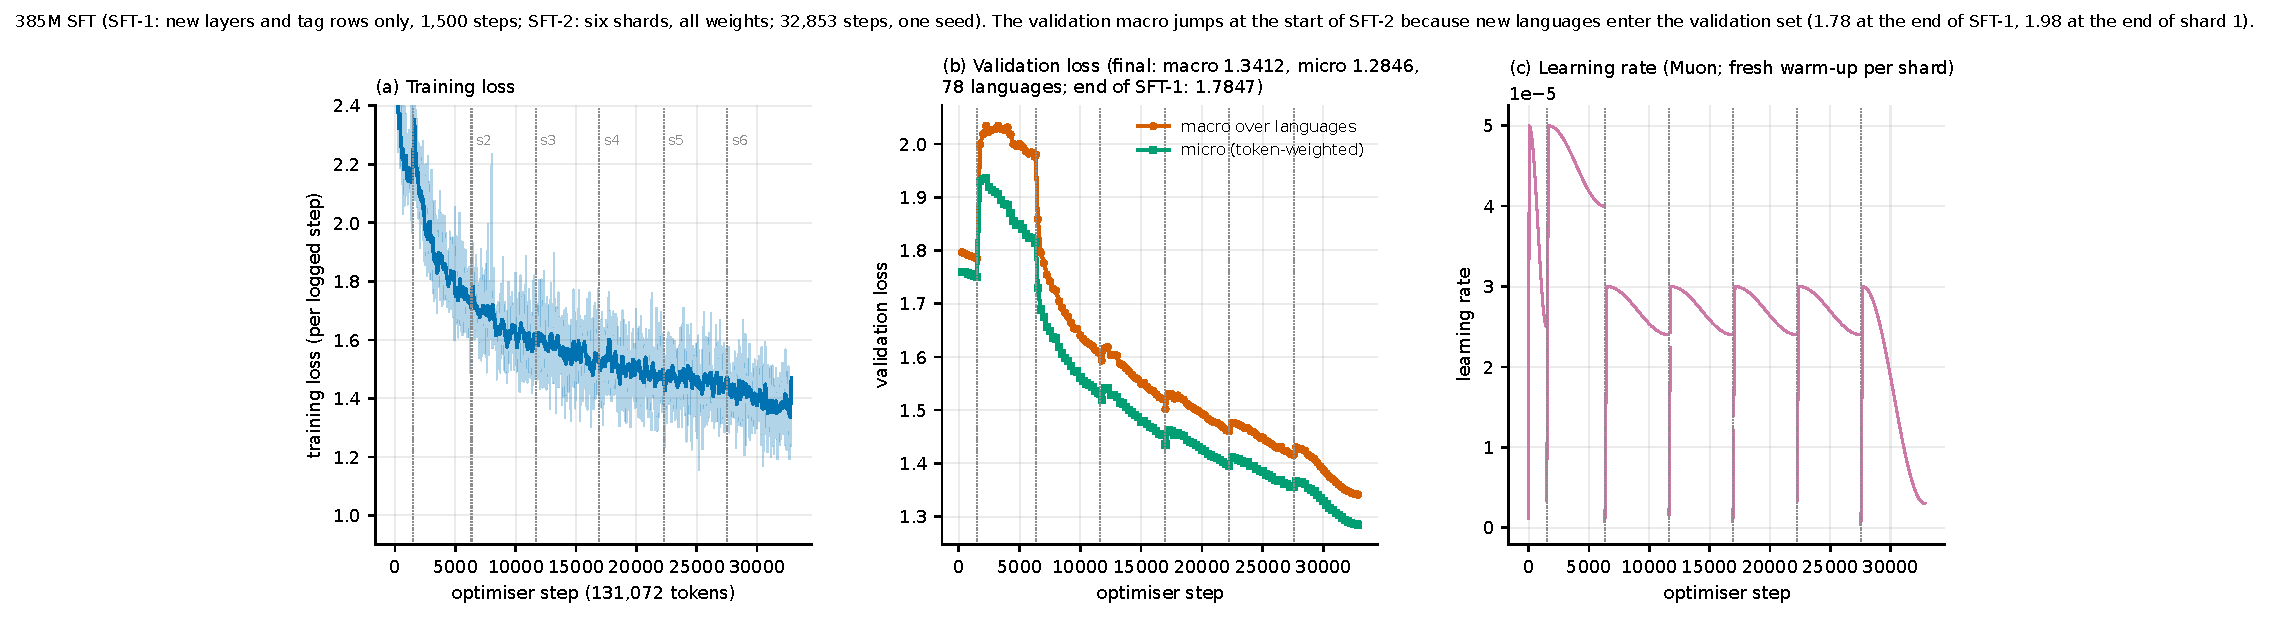
\includegraphics[width=1.00\linewidth]{figures/fig13_sft_validation_curve.pdf}
\caption{Training of the 385M SFT (one seed): (a) training loss per logged step (thin) and 20-point mean (thick), (b) validation loss (macro over languages and token-weighted micro) and (c) learning rate over the 32,853 optimiser steps of SFT-1 (1,500 steps, new layers and tag rows only) and the six SFT-2 shards (dotted lines); the validation macro jumps at the start of SFT-2 because new languages enter the validation set, and the learning-rate panel shows the per-shard schedule of Section~\ref{sec:method}. Final validation loss: macro 1.3412, micro 1.2846 over 78 languages. Source: \texttt{reports/\allowbreak{}data/\allowbreak{}e23\_\allowbreak{}hygiene\_\allowbreak{}2026-\allowbreak{}11-\allowbreak{}04/\allowbreak{}sft\_\allowbreak{}385m\_\allowbreak{}curve.\allowbreak{}csv}.}\label{fig:fig13_sft_validation_curve}
\end{figure}

\subsection{RL: optimiser, stages, prompts, reward and features}

\textbf{GRPO as used.} One on-policy update per sampled batch; a prompt gets a group of 16 completions (15 sampled plus the greedy output; in guided groups 14 sampled, the guide and the greedy output); the advantage is the group-standardised reward; the loss is the token-level policy-gradient term plus a k3 KL penalty to a reference model (coefficient 0.05 in stages A to mixed; the reference is the start model of each stage, i.e. the SFT final for stage A and the previous stage's checkpoint afterwards, because every stage restarts with a fresh reference and a fresh optimiser) \citep{shao2024deepseekmath,schulman2020approximating}. Optimiser: Muon (momentum 0.95, 5 Newton-Schulz steps), \textbf{learning rate 2e-6} with 10 warm-up steps, weight decay 0, gradient clipping 1.0; temperature 1.0, top-p 1.0; at most 384 new tokens in the short-window bin (b64) and 1,280 in b256 and the mixed stage; seed 1234. A KL guard cuts the learning rate when the median KL exceeds a threshold (0.15 in stage A, 0.25 later). Prompts per step: 64 in stage A, 48 in B1, 42 in mixed. 
% src: HYG section 3 (M7: runs_385m/{A,B1,mixed}/config.json, copies in reports/data/e23_hygiene_2026-11-04/rl_configs/); repository configs gemma_mt/configs/clean_rerun_385m/rl_A_b64.yaml, rl_B1_b256.yaml, rl_C_mixed.yaml (learning_rate 2.0e-06, kl_coef 0.05, model_name = KL reference AND policy start); reports/rl_stage_A_385m_2026-11-03.md; reports/rl_vs_sft_evidence_2026-11-04.md section 6

\begin{table}[t]
\centering\scriptsize
\setlength{\tabcolsep}{4pt}
\caption{RL hyper-parameters by stage.}\label{tab:stagecfg_full}
\begin{tabularx}{\linewidth}{@{}lrrr>{\raggedright\arraybackslash}X>{\raggedright\arraybackslash}X@{}}
\toprule
stage & learning rate & KL coefficient (k3) & group size & guide member & steps (cap) $\times$ prompts \\
\midrule
A, B1, mixed & 2e-6 (10 warm-up steps) & 0.05 & 16 (15 + greedy) & beam/MBR, fraction 0.25 (from step 41 in A) & 400 $\times$ 64; 150 (135 run) $\times$ 48; 60 $\times$ 42 \\
science RL & 1.0e-6 & 0.1 & 16 & beam/MBR, fraction 0.25 & 150 in the yaml, cap extended to 190 by the extension rule at step 120; executed 160 (stopped at step 150 by dev plateau, then 10 wind-down steps; \texttt{summary.\allowbreak{}json}, Appendix~\ref{app:chain}) $\times$ 42 \\
long-document RL & 1.0e-6 & 0.1 & 8 (7 + greedy) & off & 80 $\times$ 32 (51\% long prompts) \\
\bottomrule
\end{tabularx}
\end{table}

The science SFT before the science RL used AdamW at 3e-6 (Section~\ref{sec:science}). Dynamic-sampling, std-floor and reference-domain settings differ by stage as well (Appendix~\ref{app:chain}). 
% src: A to mixed: gemma_mt/configs/clean_rerun_385m/rl_{A_b64,B1_b256,C_mixed}.yaml. Long-document RL: gemma_mt/configs/clean_rerun_385m_long/rl_F_final.yaml (learning_rate 1.0e-06 "D-59", kl_coef 0.1, group_size 8, guide_fraction 0.0, steps 80, prompts_per_step 32, extend_if_improving false, KL reference = the start model). Science RL: `clean_rerun_385m_sci/rl_F_final.yaml` on the A100 box (the file that runs): Muon, LR 1.0e-6, KL coefficient 0.1 with the start model as reference (D-59), group 16, guide fraction 0.25, as read by the coordinator on 2026-11-04; The file is stored at reports/data/rl_configs_as_executed_2026-11-04/sci_rl_F_final.yaml (reproducibility list of the draft). Closes the LDOC "KL coef 0.1 / 1e-6" flag; the `kl_coef` comment of the long-document yaml adds that the old final run's yaml said 0.05 but its CLI override executed 0.1

\textbf{Stages.} Stage A (400 steps, short English windows, bin b64), B1 (135 steps run, b256; best checkpoint step 50 by dev chrF++), mixed (60 steps, b64 and b256), then a continued-RL run on eight weak languages (85 steps), a science SFT with weight interpolation, a science RL and a long-document RL (Appendix~\ref{app:chain}). B1 started from stage A's final model (step 400), mixed from B1's best checkpoint (step 50), the weak-group run from the mixed best, the science SFT from the mixed best. The dev set has \textbf{720 sentences = 18 FLORES+ dev languages $\times$ 40 sentences} (afr ewe fon hau ibo kin nya orm sna som sot swh tsn twi wol xho yor zul). B1's step-135 weights (\anonreal{an anonymised checkpoint}{Hub branch \texttt{stage-\allowbreak{}b1-\allowbreak{}final}}) were evaluated after the fact (E-20, Section~\ref{sec:seeds}) and equal B1 best within noise. 
% src: HYG X3, X4, X19; ledger M8. Step 200 of stage A was the dev-best checkpoint at its time (dev 40.4697); the final model of step 400 (dev 40.50, a gain of 0.03 below the selection minimum 0.1) is the one every evaluation uses

\textbf{Prompts.} English windows of consecutive sentences from FineWeb-Edu and Wikipedia (70\%) and from news (BBC, Wikinews, Global Voices, and Wikivoyage; 30\%), filtered against the protected index; 81 languages with higher draw weights for the 29 weakest. The stage-A news pool contained Wikivoyage (\texttt{darkpredator/\allowbreak{}stealth-\allowbreak{}wikivoyage-\allowbreak{}en}; 188 prompts drawn in steps 1-400) and an unlisted source \texttt{SetFit/\allowbreak{}bbc-\allowbreak{}news} (37 pool rows, none drawn). 
% src: reports/rl_prompts_news_2026-11-03.md; reports/rl_stage_A_385m_2026-11-03.md; ledger L5, CT13; CFU section 1

\textbf{Reward.} Per completion: hard failures (missing or wrong language tag, unfinished or text after the end token, copy of the source, degenerate repetition, wrong language by GlotLID \citep{kargaran2023glotlid} with a 15-character minimum, length outside the human window) receive the floor reward \ensuremath{-}2. Otherwise the content signal is a reference-free quality-estimation ensemble of \texttt{masakhane/\allowbreak{}africomet-\allowbreak{}qe-\allowbreak{}stl-\allowbreak{}1.\allowbreak{}1} \citep{wang2024africomet} (r1) and \texttt{McGill-\allowbreak{}NLP/\allowbreak{}ssa-\allowbreak{}comet-\allowbreak{}mtl} run without a reference \citep{li2025ssacomet} (r2), each shaped per language onto a monotone curve calibrated on human references (held-out calibration split of 261 ids, never dev, devtest or test). \textbf{The ensemble is the mean of the two shaped rewards if |r1 - r2| $\le$ 1.0 and the minimum otherwise}; it exists for 42 languages (41 with an ensemble block; Dyula has none). For languages without a validated QE model the content signal is the consensus (mean sentence chrF++ against the other valid group members, at least 3 valid members, blend 0.5); for five weak languages (kea kbp nus bam kab) an NLLB-3.3B pseudo-reference chrF++ term is added with weight 0.25 (max 0.35), reward only. Penalties are penalties only (never a bonus), as executed in stages A, B1 and mixed: length (weight 1.0 per log-unit outside the language's human length-ratio window, widened by 15\%), word ratio (0.5 per log-unit of the words ratio above the human 99th percentile, slack 15\%), lexical (1.0 per unit of deficit in numbers, names and content words that are not in the source), diacritics (1.0), and the constraint anchors (boilerplate, copy with cap 2.0, entity recall 0.5, function words 0.3, padding, repetition and a lexicon guard; v1 for consensus and blend languages, v2 for all three content modes; a saturated stuffing deficit at 0.9 is a hard failure); the fluency and science-anchor penalties were off; hard-failure classes also include an empty output. The reward range is [\ensuremath{-}2, 2.25]. The reward is computed per sentence chunk and aggregated by source length, with failed chunks at \ensuremath{-}2 (long-document reward \texttt{longdoc\_\allowbreak{}v2}, applied to short bins too). 
% src: HYG section 3 (M9: gemma_mt/gemma_mt/rl/qe_ensemble.py header, shaping_clean_v2.json `ens_delta` 1.0, training_state reward_range); reports/rl_vs_sft_evidence_2026-11-04.md section 1 (reward-family table); reports/rl_stage_plan_385m_b256_2026-11-02.md section 3; penalty list read from the reward code and the executed configs (`research_archive_2026-11-03/box_final_2026-11-04/clean_rerun/tree/gemma_mt/gemma_mt/rl/reward.py`; `reports/data/e23_hygiene_2026-11-04/rl_configs/config_{A,B1,mixed}.json`, identical reward block in A, B1 and mixed)

\textbf{Four features added at step 41 of stage A.} Stage A ran steps 1-40 without them; at the step-40 checkpoint the trainer was stopped and resumed from \texttt{last/\allowbreak{}} with all four switched on. (1) Dynamic sampling: oversample 1.1 (later 1.0), drop flat groups, refill up to twice \citep{yu2025dapo}; (2) an advantage standard-deviation floor of 0.02; (3) a beam-guided group member: for 25\% of the prompts the beam-4 output (or, for 31 weak languages, an MBR winner over 16 extra samples; skipped on 99\% of B1 steps for cost) replaces the last sampled member, with ratio 1 and the guides' advantage share capped at 0.25; (4) a reference-anchored term on 15\% of the prompts (7 languages: amh efi hau lug nso yor zul, human pairs from AfriScience-MT train and IbomMT train): r = 0.65 r\_existing + 0.35 consensus\_value(chrF++ against the human reference). In stage A the std floor never bound (group-std p10 0.128 against 0.02) and dynamic sampling never acted (flat fraction 0); the beam guide cost a median 26.6\% of step time and was above the mean of the other members in 83\% of groups. The stage-A log cannot separate the four features, so we ablated them at 100 steps (E-11, Appendix~\ref{app:split}): together they are worth a small gain (+0.32 chrF++), mostly the reference-anchored term, the beam guide is not shown to be worth its 25\% step time, and none of them causes the KL rise; we describe them as design choices, not as contributions. The archived stage-A \texttt{config.\allowbreak{}json} is the resumed (post step 40) configuration, so the values of steps 1-40 are known only from the stage report. 
% src: reports/rl_features_dynamic_ref_2026-11-03.md; reports/rl_stage_A_385m_2026-11-03.md; HYG X18; SPLIT

\textbf{Learning rate in stage A.} The KL guard cut the learning rate at steps 226 (x0.5), 236 (x0.25) and 247 (x0.125) and it never recovered: steps 247-400 ran at 2.5e-7 instead of 2e-6. The dev curve was flat from about step 100, before the first cut. 
% src: reports/rl_stage_A_385m_2026-11-03.md Optimisation; SPLIT

\textbf{Monitors and stops.} From the mixed stage on, the held-out reference-based \texttt{masakhane/\allowbreak{}africomet-\allowbreak{}stl-\allowbreak{}1.\allowbreak{}1} is scored at every dev evaluation (never a reward) and enters a hacking alarm (QE rising while dev chrF++ falls by more than 0.75 and AfriCOMET by more than 0.03) and a combined dev-plateau stop (two dev evaluations, 50 steps, without a gain of 0.15 chrF++ or 0.004 AfriCOMET). 
% src: reports/rl_features_dynamic_ref_2026-11-03.md section 14, 17

\textbf{Cost.} Stage A 15,920 s for 400 steps (39.8 s per step), B1 10,479 s for 135 steps, mixed 4,786 s for 60 steps; the chain is 8.66 A100-hours. 
% src: reports/rl_vs_sft_evidence_2026-11-04.md section 6

\section{SFT against A0 and the earlier 270M work (details)}\label{app:sft}

\begin{table}[t]
\centering\small
\setlength{\tabcolsep}{4pt}
\caption{chrF++ of the 385M SFT against A0 (language macro, all rows; 95\% paired bootstrap). Language counts differ between benchmarks.}\label{tab:sft_a0}
\begin{tabularx}{\linewidth}{@{}lrr>{\raggedright\arraybackslash}X@{}}
\toprule
benchmark (languages) & chrF++ 385M SFT & chrF++ A0 & delta [95\% CI] \\
\midrule
FLORES+ devtest (46) & 25.52 & 20.20 & +5.31 [+5.13, +5.50] \\
NTREX-128 (24) & 29.25 & 23.01 & +6.24 [+6.02, +6.45] \\
MAFAND-MT test (15) & 35.77 & 25.56 & +10.21 [+9.90, +10.54] \\
SmolSent (45) & 22.53 & 17.18 & +5.36 [+5.14, +5.60] \\
SALT (5) & 35.49 & 25.13 & +10.36 [+9.29, +11.44] \\
GlotStoryBook (8) & 20.22 & 14.62 & +5.59 [+4.92, +6.21] \\
IbomMT (2) & 12.04 & 9.87 & +2.16 [+1.58, +2.74] \\
FLORES-MOZ (1) & 21.54 & 21.08 & +0.46 [\ensuremath{-}0.72, +1.73] \\
\bottomrule
\end{tabularx}
\end{table}

On FLORES+ 38 of 46 languages are significantly better, 6 are not different (kab orm lua lug seh nso) and 2 are worse (kea \ensuremath{-}17.56 [\ensuremath{-}18.96, \ensuremath{-}16.10], dyu \ensuremath{-}2.33 [\ensuremath{-}3.06, \ensuremath{-}1.60]). Held-out AfriCOMET is significantly better for every language that has it (FLORES+ 0.554 against 0.442). The comparison confounds depth with the additional SFT (stage B, 40 added languages, NLLB-mined/Aya/Tumbuka data). Kabuverdianu falls from 36.47 to 18.91 with finished rate 0.98 $\to$ 0.83 and 82\% NLLB-mined stage-B tokens; its cause is untested. 
% src: EVAL T1, T10, section 3; NLLBLINK section 4

On exactly the sentences the old 270M models had not seen, the 385M SFT is behind the old SFT on seven of eight benchmarks (FLORES+ 22.34 against 25.06, NTREX 27.35 against 31.46, MAFAND 34.80 against 38.18, SmolSent 17.03 against 19.97, SALT 30.60 against 33.58, IbomMT 9.49 against 13.96, FLORES-MOZ 19.72 against 22.96; GlotStoryBook 20.27 against 19.85). The block of Sotho-Tswana, Tsonga, hau, run, kin, ssw, orm, kab regresses most (lug \ensuremath{-}15.3, nso \ensuremath{-}15.3, tso \ensuremath{-}14.8, sot \ensuremath{-}11.7). The regression already exists with A0, which has no NLLB-mined rows; the link to NLLB share is inconclusive (Appendix~\ref{app:nllblink}). 
% src: EVAL section 4, T3b; NLLBLINK sections 1-2. Old-model numbers come from earlier runs of the same harness in a different code state and have no intervals; the E-13 rerun below replaces them for FLORES+, NTREX and MAFAND

\textbf{Same harness (E-13).} The earlier 270M work's 270M SFT and RL-final (rl2c) were generated again with the 385M harness (greedy, 768 tokens, vLLM bf16) and compared with the 385M SFT and RL (mixed best) on rows that are clean for both generations, with a paired bootstrap (1,000 resamples, 95\% CI). 

\begin{table}[t]
\centering\footnotesize
\setlength{\tabcolsep}{4pt}
\caption{chrF++ of the earlier 270M work's 270M SFT and RL-final (rl2c) re-run in the 385M harness (E-13), against the 385M SFT and RL (mixed best), on rows clean for both generations; language macro.}\label{tab:t_old270m}
\begin{tabularx}{\linewidth}{@{}>{\raggedright\arraybackslash}Xrrlrrl@{}}
\toprule
benchmark (languages) & old 270M SFT & 385M SFT & 385M SFT - old SFT & old 270M RL (rl2c) & 385M RL & 385M RL - old RL \\
\midrule
FLORES+ devtest (45) & 24.69 & 22.34 & \ensuremath{-}2.35 [\ensuremath{-}3.25, \ensuremath{-}1.38] & 31.68 & 32.03 & +0.35 [+0.08, +0.62] \\
NTREX (24) & 31.46 & 27.33 & \ensuremath{-}4.13 [\ensuremath{-}4.40, \ensuremath{-}3.85] & 35.52 & 35.55 & +0.02 [\ensuremath{-}0.07, +0.11] \\
MAFAND (15) & 38.26 & 34.71 & \ensuremath{-}3.54 [\ensuremath{-}4.22, \ensuremath{-}2.75] & 41.80 & 40.25 & \ensuremath{-}1.55 [\ensuremath{-}1.72, \ensuremath{-}1.39] \\
\bottomrule
\end{tabularx}
\end{table}

 The 385M SFT is behind the old SFT on all three benchmarks and on held-out AfriCOMET (\ensuremath{-}0.0113 [\ensuremath{-}0.0189, \ensuremath{-}0.0037], \ensuremath{-}0.0250 [\ensuremath{-}0.0273, \ensuremath{-}0.0229], \ensuremath{-}0.0158 [\ensuremath{-}0.0188, \ensuremath{-}0.0130]); after RL the 385M model is level with the old RL on FLORES+ and NTREX in chrF++ and 1.55 chrF++ below it on MAFAND, and lower on AfriCOMET on all three (\ensuremath{-}0.0051 [\ensuremath{-}0.0104, \ensuremath{-}0.0001], \ensuremath{-}0.0129 [\ensuremath{-}0.0144, \ensuremath{-}0.0115], \ensuremath{-}0.0203 [\ensuremath{-}0.0222, \ensuremath{-}0.0182]). The rerun reproduces the stored old-model numbers to within 0.4 chrF++ (old SFT FLORES+ 24.69 against 25.06). Caveats: the clean-for-both filter keeps 2,160 of 45,540 FLORES+ rows (4.7\%; 48 sentences per language) and 28,680 of 47,928 NTREX rows, so these 385M numbers are on a different row set from those of Section~\ref{sec:rlsft}; the generations differ in data, steps, tokenizer layout, reward and code state; one seed per model; SmolSent, SALT, GlotStoryBook, IbomMT and FLORES-MOZ were not re-run for the old models (the earlier ``7 of 8 benchmarks'' statement is not re-measured for those five).
% src: reports/e13_old270m_same_harness_2026-11-04.md; reports/data/e13_old270m_same_harness_2026-11-04/evidence_e13.json (`stages`; ledger S7b, R16b)

\begin{figure}[t]
\centering
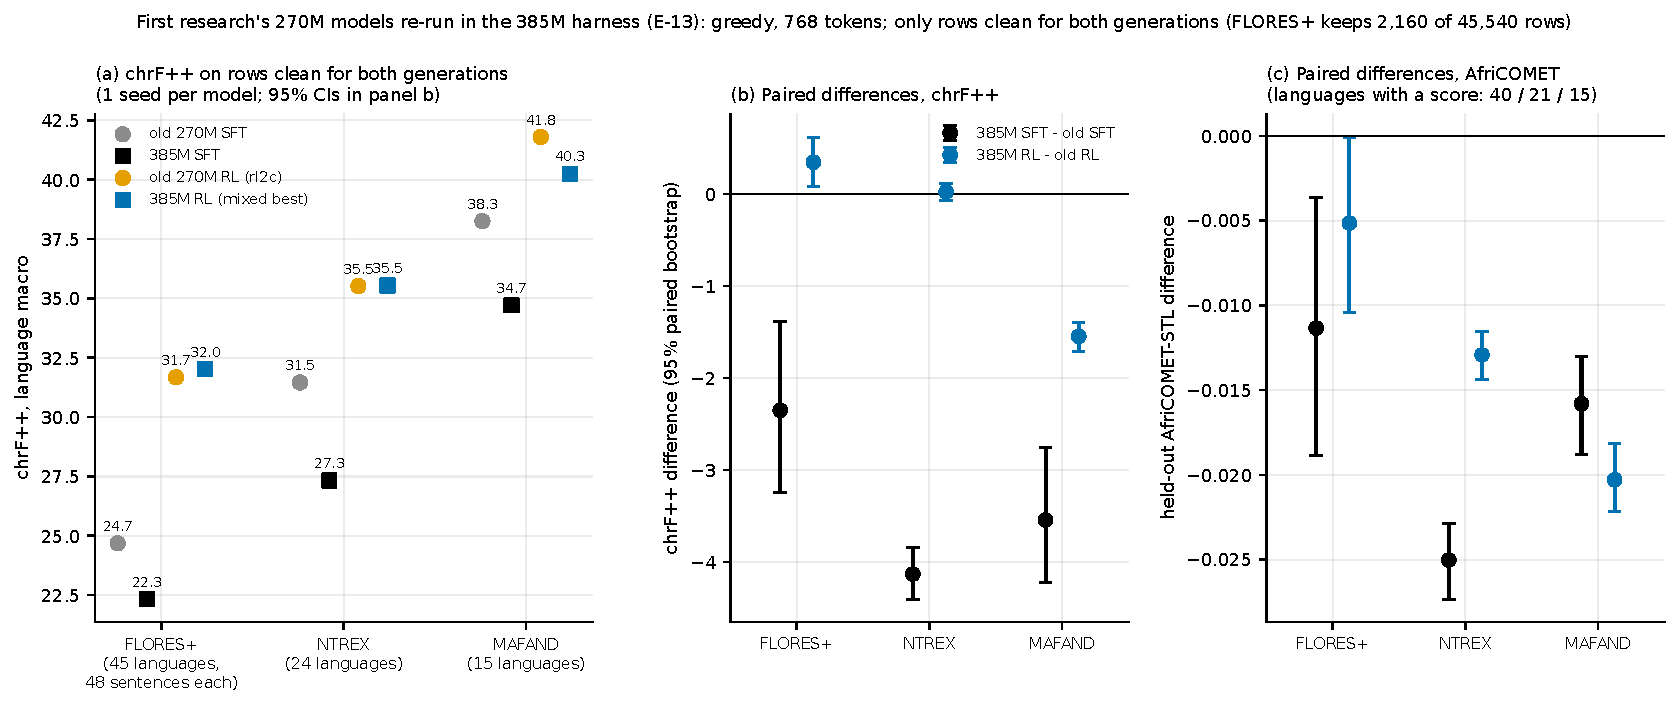
\includegraphics[width=1.00\linewidth]{figures/fig10_old270m_same_harness.pdf}
\caption{The earlier 270M work's 270M models re-run in the 385M harness (E-13): (a) language-macro chrF++ of the old 270M SFT and RL-final (rl2c) and the 385M SFT and RL (mixed best) on FLORES+ devtest (45 languages, 48 sentences each), NTREX (24) and MAFAND (15), rows clean for both generations only; (b) paired differences with 95\% bootstrap over sentences (Poisson weights; 1,000 resamples); (c) the same for held-out AfriCOMET-STL (languages with a score: 40 / 21 / 15). One seed per model. Source: \texttt{reports/\allowbreak{}data/\allowbreak{}e13\_\allowbreak{}old270m\_\allowbreak{}same\_\allowbreak{}harness\_\allowbreak{}2026-\allowbreak{}11-\allowbreak{}04/\allowbreak{}evidence\_\allowbreak{}e13.\allowbreak{}json}.}\label{fig:fig10_old270m_same_harness}
\end{figure}

\subsection{Weak and added languages}\label{app:weaklangs}

After SFT, 37 of 74 scored languages are weak (chrF++ < 14 or finished rate < 0.9), 16 of them by chrF++: shi 0.2, ibb 2.3, zgh 2.3, dag 2.4, aeb 2.8, taq 2.8, dik 3.8, knc 3.8, arz 4.6, ary 4.6, dyu 9.9, tir 10.5, cjk 10.7, orm 12.1, tiv 13.3, nus 13.5. Of the nine languages that the SFT report lists as added (the eight on FLORES+ that are among the 40 registry rows appended after A0, plus seh, which the registry counts among the first 85 rows), mfe (28.5) and seh (21.7) work, cjk (10.7) is weak, and arz, ary, dik, aeb, taq and zgh fail (English or Modern Standard Arabic output, token loops).  After RL (mixed best): mfe 37.93, cjk 23.02, dik 14.06, taq 11.06, arz 9.18, ary 6.88, aeb 4.12, zgh 4.07.  Arabic dialects, Tamazight, Dinka, Tamasheq and Kanuri (knc) are not usable after RL (chrF++ 2 to 14; loops in 11\% to 56\% of FLORES+ outputs by the reward's flag, and an English-output share of up to 0.5 in aeb and ary, Section~\ref{sec:degen}).
% src: EVAL section 6, T5
% src: EVID Table 6

\begin{figure}[t]
\centering
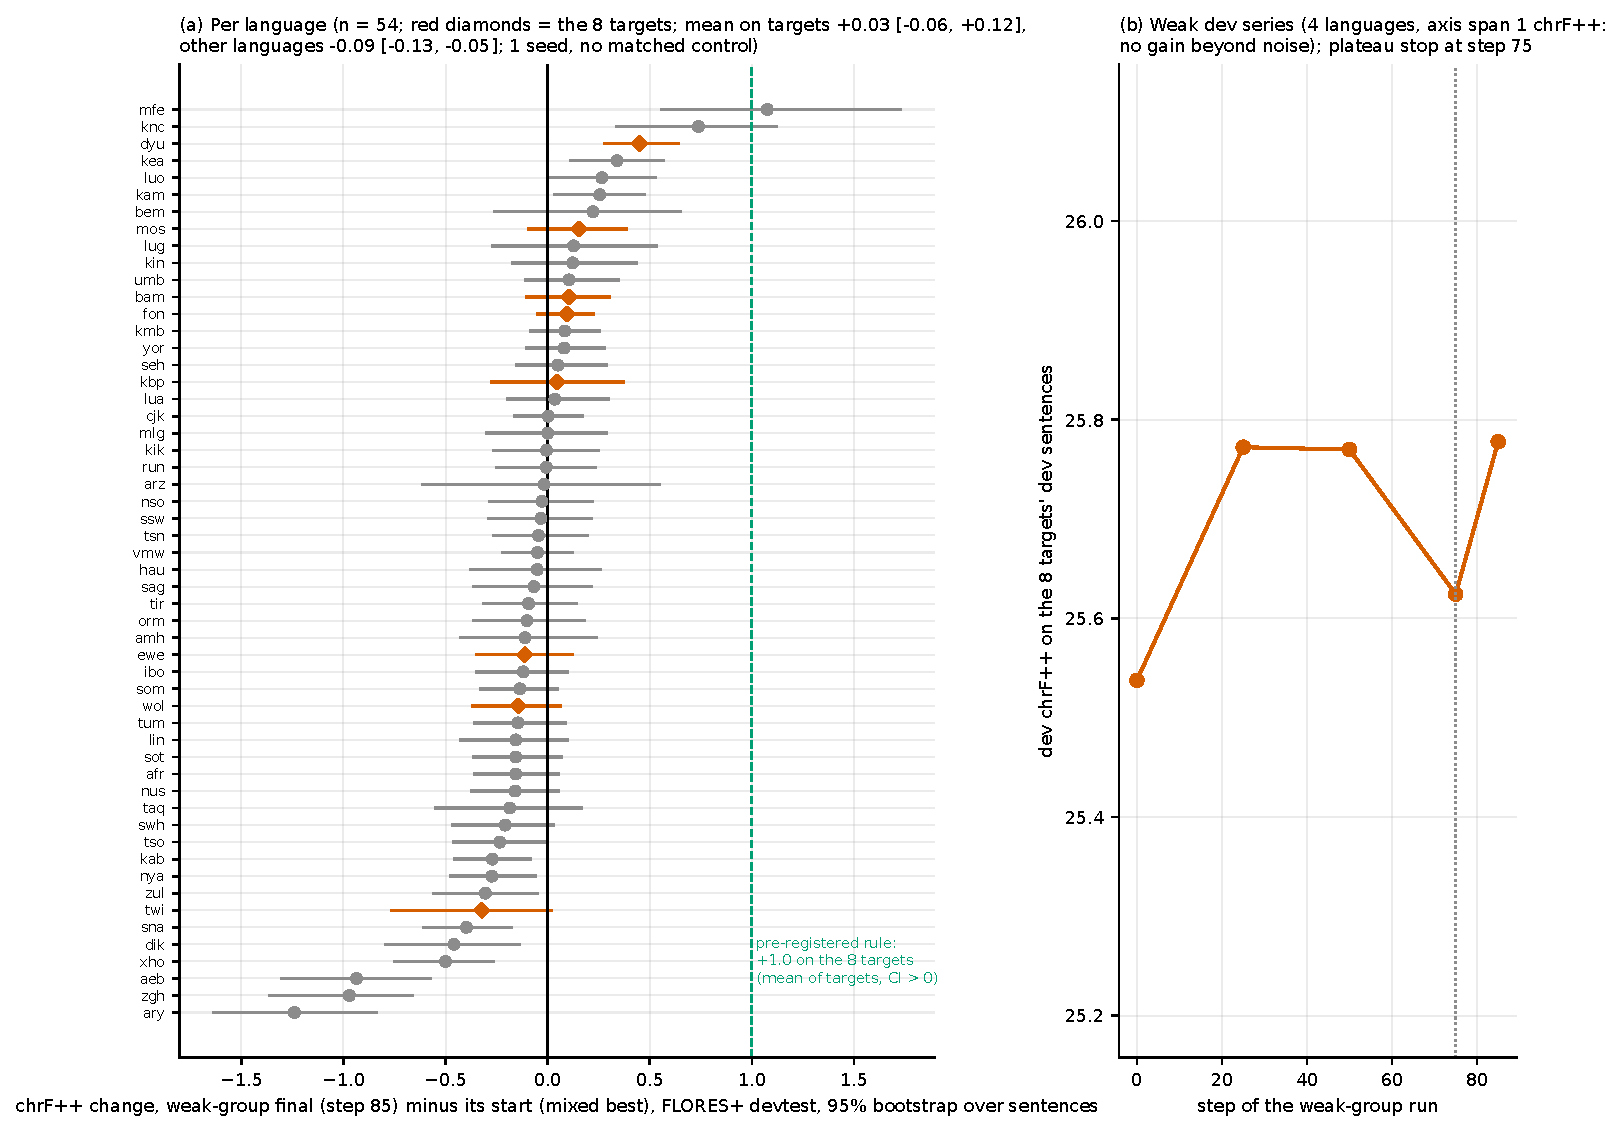
\includegraphics[width=0.90\linewidth]{figures/fig6_weak_group.pdf}
\caption{(a) Continued RL on eight weak West-African languages (mos fon kbp bam wol ewe twi dyu; 85 steps, 2.1 GPU-hours): chrF++ change of the final (step 85) against its start, the mixed best, per FLORES+ language (n = 54; 1,012 sentences each; 95\% bootstrap over sentences; one seed, no matched control). Red diamonds are the targets: mean +0.03 [\ensuremath{-}0.06, +0.12] against the pre-registered +1.0; the 46 other languages move by \ensuremath{-}0.09 [\ensuremath{-}0.13, \ensuremath{-}0.05]. (b) The run's own dev series on the targets' dev sentences (axis span 1 chrF++; dev evaluation noise is sd 0.09 to 0.10). Sources: \texttt{reports/\allowbreak{}data/\allowbreak{}eval\_\allowbreak{}weak\_\allowbreak{}group\_\allowbreak{}2026-\allowbreak{}11-\allowbreak{}03/\allowbreak{}scores/\allowbreak{}bootstrap\_\allowbreak{}by\_\allowbreak{}language.\allowbreak{}csv}, \texttt{research\_\allowbreak{}archive\_\allowbreak{}2026-\allowbreak{}11-\allowbreak{}03/\allowbreak{}clean\_\allowbreak{}rerun\_\allowbreak{}misc/\allowbreak{}runs\_\allowbreak{}385m\_\allowbreak{}weak/\allowbreak{}mixed/\allowbreak{}metrics.\allowbreak{}jsonl}.}\label{fig:weakgroup}
\end{figure}

\section{RL chain: stage summary, B1 final and training records}\label{app:chain}

\begin{table}[t]
\centering\scriptsize
\setlength{\tabcolsep}{4pt}
\caption{Stage chain summary (not all rows are FLORES+ stages).}\label{tab:chain_full}
\begin{tabularx}{\linewidth}{@{}>{\raggedright\arraybackslash}X>{\raggedright\arraybackslash}X>{\raggedright\arraybackslash}X>{\raggedright\arraybackslash}X@{}}
\toprule
stage & steps run & cost & result on FLORES+ chrF++ (vs previous stage) \\
\midrule
SFT-1 / SFT-2 (A0 $\to$ 385M) & 1,500 + 31,353 & 44.8 h for stage B (A100) & 22.85 (SFT, 54 languages) \\
continued-SFT control (E-03; not an RL stage) & 6,000 & 8.4 h (5.05 s/step), RL chain 8.66 h & FLORES+ 25.38 (+2.53 over the SFT [+2.35, +2.71]); 93 cells 29.97 against 34.55 for the mixed best \\
RL stage A & 400 & 15,920 s (4.42 h) & 30.81 (+7.96) \\
RL B1 & 135 (best step 50) & 10,479 s & 31.35 (+0.54) \\
RL mixed & 60 & 4,786 s & 31.66 (+0.31) \\
weak-group RL (8 languages) & 85 (plateau stop at 75) & 2.1 GPU-h & targets +0.03 [\ensuremath{-}0.06, +0.12]; other languages \ensuremath{-}0.09 [\ensuremath{-}0.13, \ensuremath{-}0.05] \\
science SFT & 283 (65,536 tokens) & 17 min & AfriScience chrF +1.2; SSA-COMET-QE flat \\
science RL & 160 steps executed (cap 150 in the yaml, extended to 190 at step 120; dev plateau at step 150 plus 10 wind-down steps; \texttt{summary.\allowbreak{}json} stop reason \texttt{dev\_\allowbreak{}plateau}; best at step 75) & not stated in the evaluation report & AfriScience test (6 languages), final vs start: chrF +0.46 [+0.27, +0.65], held-out AfriCOMET +0.0053 [+0.0036, +0.0071], SSA-COMET-QE +0.0041 (reward family); NTREX +0.42, MAFAND +0.10 chrF++; no document-level gain (not a FLORES+ stage) \\
science RL without the science SFT (E-14) & 160 (150 + 10 wind-down; one OOM restart from step 20; final only) & about 5 h wall-clock (15:18 to 20:17 UTC; 14,395 s in the last process) & AfriScience test chrF 45.66 (start 45.40; science RL from the science SFT 47.10); 93-cell chrF++ +0.13 over the mixed best (not a FLORES+ stage) \\
long-document RL & 80 (best at step 50; no extension) & 7.7 h wall-clock, of which about 4.5 h a crash loop (Appendix~\ref{app:repro}) & whole-document finished +0.125, loop \ensuremath{-}0.113, chrF +3.4; chunked and sentence level unchanged (not a FLORES+ stage) \\
\bottomrule
\end{tabularx}
\end{table}

% GATE E-03: the cost column is the compute the control must match
% src: reports/rl_vs_sft_evidence_2026-11-04.md section 6 (cost); EVID Table 3; reports/eval_weak_group_385m_2026-11-03.md; reports/eval_science_sft_385m_2026-11-04.md; LDOC section 2 (planned values). Science RL length: the yaml labels 150 steps a HARD CAP, but `extend_if_improving` (the trainer's extension rule: at the cap, if the improvement criterion fired within the last `extend_recent` steps, raise the cap) raised it by 40 steps to 190 while the dev metrics were still improving; the long-document yaml sets `extend_if_improving: false`. The stage A to mixed yamls also carry the extension rule (extend_steps 15, at most +50%). The executed count is reported from the run log and must be confirmed from `summary.json` when the run ends. The RL chain A + B1 + mixed is 8.66 A100-hours, of which B1's 85 steps after its best checkpoint are unused by the final model

 Stage A accounts for 94\% of the SFT-to-B1 gain on FLORES+ (7.96 of 8.50) and 96\% on NTREX; it also accounts for most of the improvement in finishing and looping (FLORES+ finished 0.829 $\to$ 0.983, loop 0.209 $\to$ 0.068; final 0.995, 0.048; Section~\ref{sec:rlsft}). We did not split the part beyond finishing by stage. The stage-A dev chrF++ (720 sentences) moves 36.81 $\to$ 39.04 (step 50) $\to$ 40.14 (100) $\to$ 40.47 (200) $\to$ 40.50 (400), with +3.3 of +3.7 in the first 100 steps; the plateau begins before the three KL-guard cuts (steps 226, 236, 247).  The later stages differ from stage A in more than step count (bin, reference domain, guides), and the later steps are small. Two extra seeds of the stage-A recipe (E-04, 100 steps, 20 languages, standard harness; Appendix~\ref{app:split}) differ by 0.06 chrF++ [\ensuremath{-}0.02, +0.14] (0.0008 AfriCOMET). On those 20 languages the stored B1 best is +0.17 [+0.12, +0.21] chrF++ over stage A, about three times the seed difference, while the mixed best is +0.07 [+0.02, +0.11] over B1 best, the size of the seed difference: \textbf{we do not call the mixed step a gain}; stage A to mixed is +0.23 [+0.18, +0.29]. These are indications from one pair of seeds at step 100, not tests of the later stages. 
% src: EVID Table 3; arithmetic checked in HYG X16
% src: STA; HYG X4
% src: reports/e04_rl_seeds_2026-11-05.md section 2; ledger E04 rows

\textbf{B1 best against B1 final (E-20).} The B1 final weights (step 135; \anonreal{an anonymised checkpoint}{Hub branch \texttt{stage-\allowbreak{}b1-\allowbreak{}final}}) were evaluated on the same 122,585 rows as every other stage (greedy, 768 tokens, language macro, 95\% paired bootstrap, one seed). 
% src: reports/e20_b1_final_2026-11-04.md; reports/data/e20_b1_final_2026-11-04/evidence_e20.json (ledger M8b)

\begin{table}[t]
\centering\footnotesize
\setlength{\tabcolsep}{4pt}
\caption{B1 final (step 135) against B1 best (step 50) and neighbouring stages; \chrfpp{}, language macro, 95\% paired bootstrap.}\label{tab:e20}
\begin{tabularx}{\linewidth}{@{}>{\raggedright\arraybackslash}Xllll@{}}
\toprule
comparison & FLORES+ chrF++ & NTREX chrF++ & MAFAND chrF++ & all 93 cells chrF++ \\
\midrule
B1 final minus B1 best & +0.04 [+0.00, +0.08] & \ensuremath{-}0.00 [\ensuremath{-}0.05, +0.05] & \ensuremath{-}0.09 [\ensuremath{-}0.15, \ensuremath{-}0.01] & +0.01 [\ensuremath{-}0.02, +0.04] \\
B1 final minus stage A & +0.58 [+0.53, +0.64] & +0.30 [+0.24, +0.36] & \ensuremath{-}0.09 [\ensuremath{-}0.17, +0.00] &  \\
mixed best minus B1 final & +0.26 [+0.22, +0.30] & +0.19 [+0.14, +0.23] & +0.05 [\ensuremath{-}0.01, +0.12] &  \\
\bottomrule
\end{tabularx}
\end{table}

Held-out AfriCOMET, B1 final minus B1 best, all cells: +0.0004 [+0.0000, +0.0008]; FLORES+ finished / loop 0.993 / 0.054 (B1 best) and 0.996 / 0.052 (B1 final). The 85 steps after step 50 changed nothing measurable, so the choice between B1 best and final does not matter for the numbers of this paper; 11 of 93 cells are significantly worse and 8 significantly better, by 0.1 to 0.3 chrF++, which is a rough noise floor for the stage-to-stage steps. (A table, not a figure, because the content is three differences.)

\begin{figure}[t]
\centering
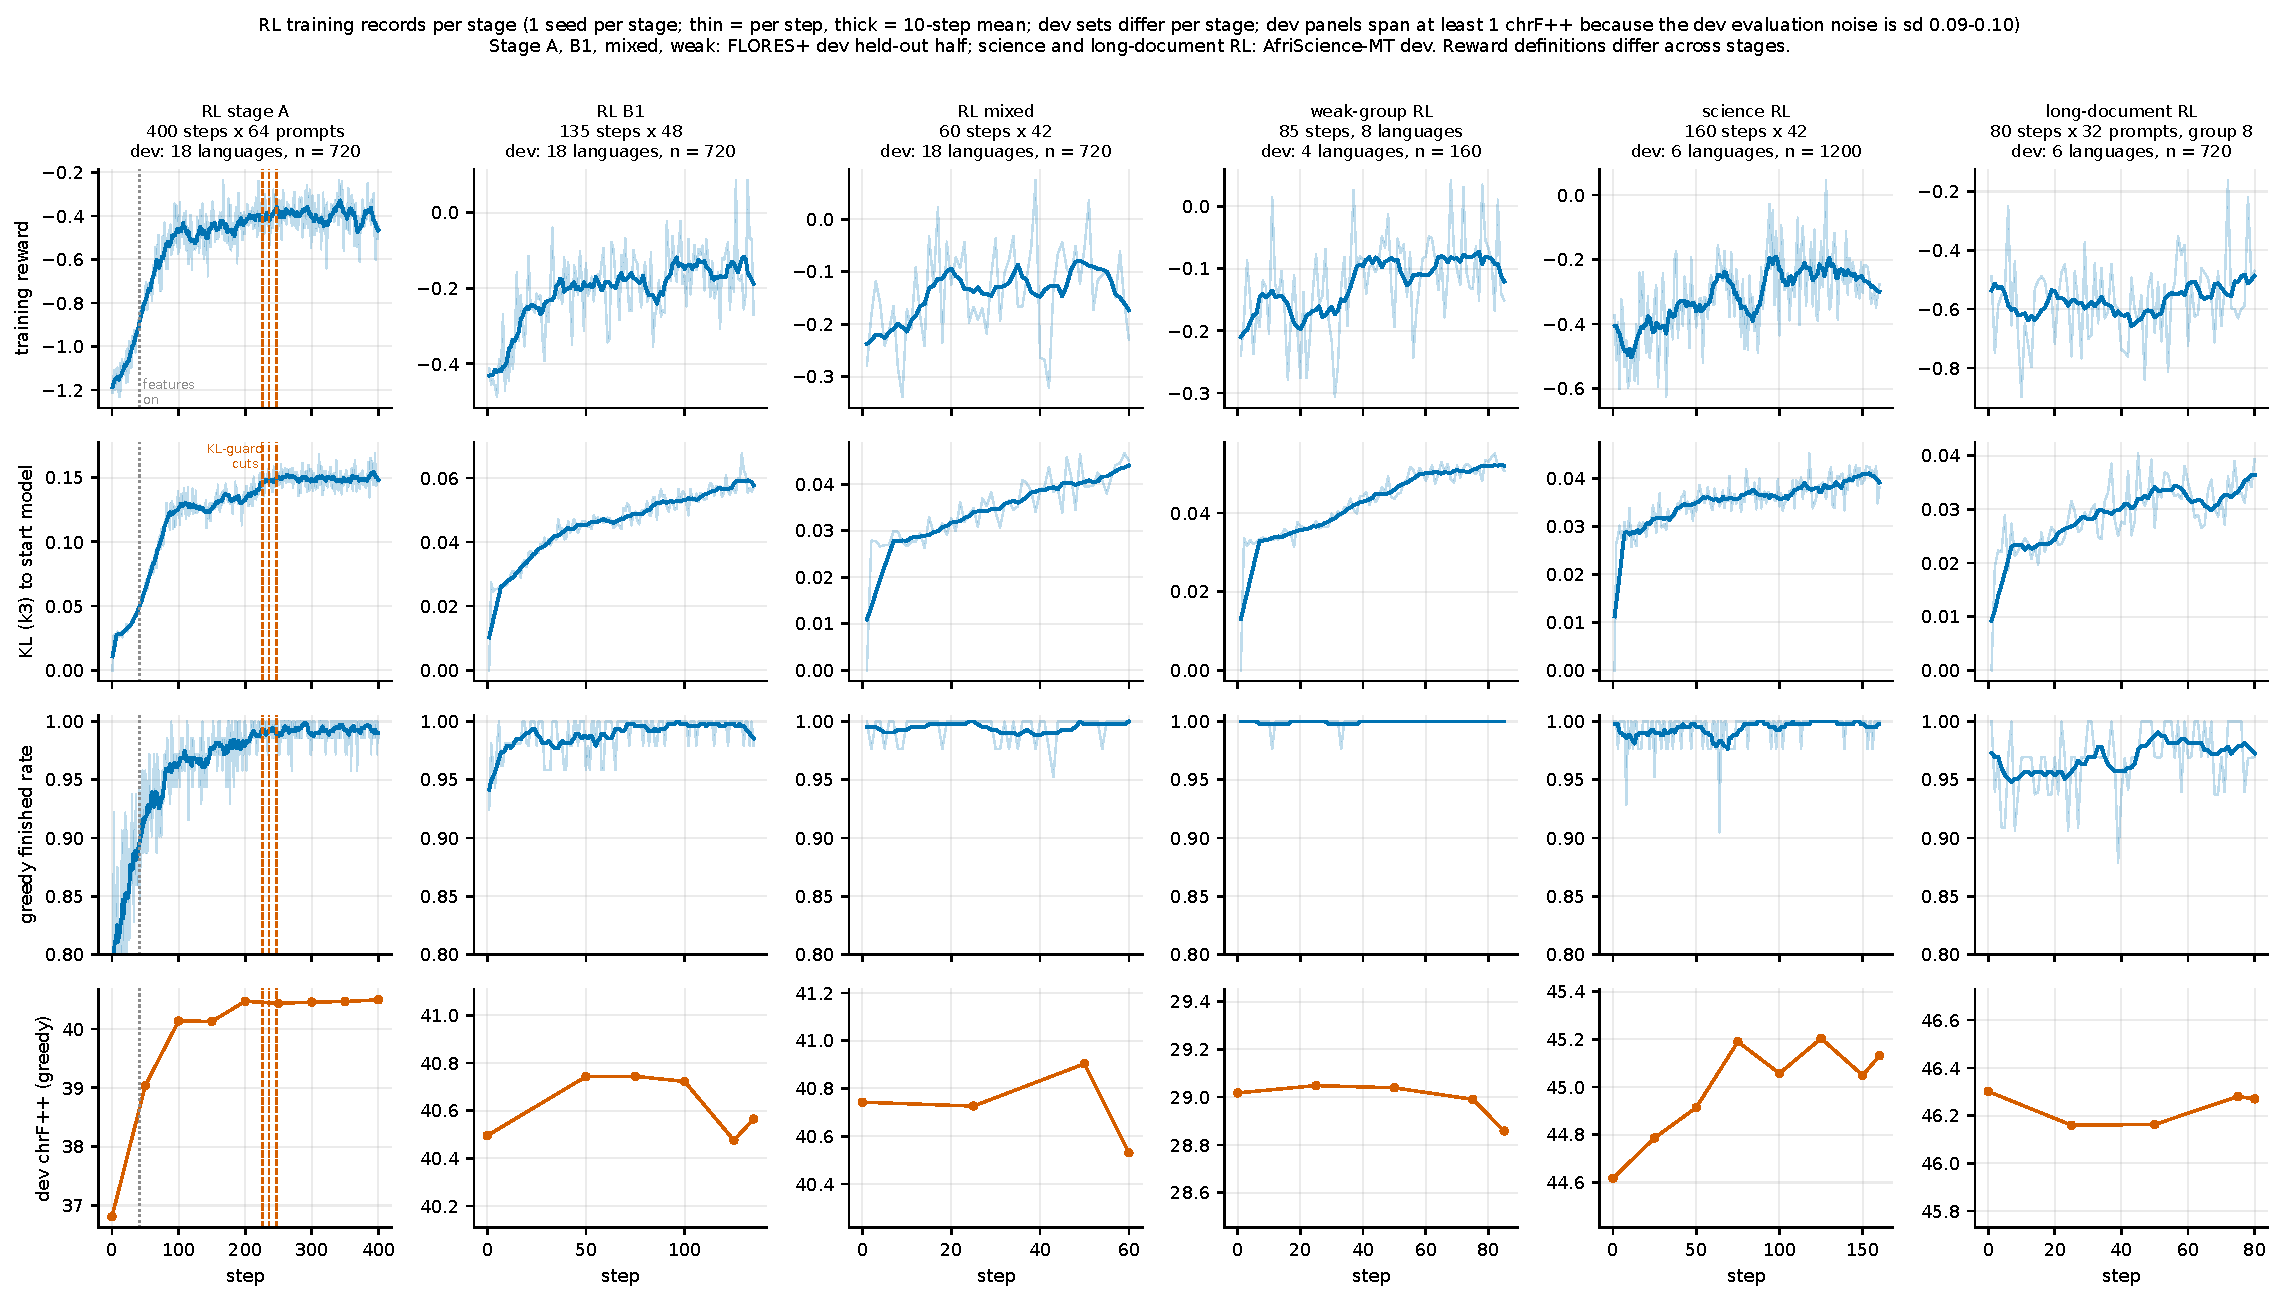
\includegraphics[width=1.00\linewidth]{figures/fig2_rl_training_curves.pdf}
\caption{Training records of every RL stage from the run logs (one seed per stage): training reward, KL (k3) to the stage's start model, finished rate of the greedy group member, and dev chrF++ against the step (thin lines per step, thick lines 10-step means). Stage A: dotted line at step 41 (four features on), dashed lines at the three KL-guard cuts (226, 236, 247). The dev sets differ by stage (FLORES+ dev held-out half for stage A, B1, mixed and weak; AfriScience-MT dev for science and long-document RL; the number of languages and sentences is in each title) and the reward definitions differ, so columns are not comparable; dev panels span at least 1 chrF++ because the dev evaluation noise is sd 0.09 to 0.10. The long-document RL log shows the 80 planned steps; step 25 was evaluated repeatedly after the crash restarts of Appendix~\ref{app:repro} and the last evaluation is shown (steps 21 to 25 were repeated by the restarts). Sources: \texttt{research\_\allowbreak{}archive\_\allowbreak{}2026-\allowbreak{}11-\allowbreak{}03/\allowbreak{}runs\_\allowbreak{}385m/\allowbreak{}\{A,B1,mixed\}/\allowbreak{}metrics.\allowbreak{}jsonl}, \texttt{clean\_\allowbreak{}rerun\_\allowbreak{}misc/\allowbreak{}runs\_\allowbreak{}385m\_\allowbreak{}\{weak/\allowbreak{}mixed,sci/\allowbreak{}final,long/\allowbreak{}final\}/\allowbreak{}metrics.\allowbreak{}jsonl}.}\label{fig:fig2_rl_training_curves}
\end{figure}

\section{RL against SFT and the control: details}\label{app:rlsft}

\begin{table}[t]
\centering\footnotesize
\setlength{\tabcolsep}{4pt}
\caption{Finished rate / loop rate (reward's flag) / hypothesis-to-reference length, clean rows, language macro.}\label{tab:finish}
\begin{tabularx}{\linewidth}{@{}l>{\raggedright\arraybackslash}Xll@{}}
\toprule
system & FLORES+ finished / loop / hyp-to-ref length & NTREX & MAFAND \\
\midrule
SFT & 0.829 / 0.209 / 3.03 & 0.890 / 0.122 / 2.35 & 0.963 / 0.043 / 1.48 \\
RL stage A & 0.983 / 0.068 / 1.33 & 0.996 / 0.016 / 1.07 & 0.999 / 0.003 / 1.00 \\
RL B1 best & 0.993 / 0.054 / 1.17 & 0.999 / 0.009 / 1.02 & 1.000 / 0.001 / 0.99 \\
RL mixed best & 0.995 / 0.048 / 1.14 & 0.999 / 0.006 / 1.02 & 1.000 / 0.001 / 0.98 \\
\bottomrule
\end{tabularx}
\end{table}

 The loop detector in this table is the reward's own guard (\texttt{is\_\allowbreak{}repetitive}, \texttt{is\_\allowbreak{}self\_\allowbreak{}repetitive}); on the human references it fires on 0.0001 of FLORES+ rows. 95\% of the RL model's flagged FLORES+ rows come from seven near-failed languages (taq knc zgh dik aeb arz ary). Section~\ref{sec:degen} tests this flag against a detector that is not the reward's.
% src: EVID Table 2

\begin{table}[t]
\centering\footnotesize
\setlength{\tabcolsep}{4pt}
\caption{RL minus SFT over the 93 cells under four ways of removing the finishing effect (clean rows; 95\% CI).}\label{tab:decomp}
\begin{tabularx}{\linewidth}{@{}>{\raggedright\arraybackslash}X>{\raggedright\arraybackslash}X>{\raggedright\arraybackslash}X@{}}
\toprule
row set & chrF++ RL - SFT [95\% CI] & AfriCOMET RL - SFT [95\% CI] (76 cells) \\
\midrule
all clean rows & +7.96 [+7.82, +8.12] & +0.0631 [+0.0620, +0.0643] \\
SFT output cut at its first loop (RL as is) & +4.06 [+3.97, +4.15] & not scorable \\
rows where the SFT finished and did not loop & +2.41 [+2.33, +2.49] & +0.0366 [+0.0357, +0.0374] \\
rows where both finished and neither loops & +2.61 [+2.54, +2.70] & +0.0370 [+0.0362, +0.0379] \\
rows where the SFT failed (21\% of FLORES+ rows) & +24.57 [+24.26, +24.90] (SFT 5.95, RL 30.53) & +0.3342 [+0.3295, +0.3391] \\
\bottomrule
\end{tabularx}
\end{table}

 Cutting the SFT's looping outputs at the loop onset (no change to the translation) raises the SFT from 26.59 to 30.49 chrF++, i.e. \textbf{49\% of the gain is recovered by cutting loops}; 67 to 70\% of the chrF++ gain is attributable to rows where either model failed; about 41\% of the AfriCOMET gain is finishing. What remains is +2.4 to +4.1 chrF++ and +0.037 AfriCOMET, significant in 50 of 54 FLORES+ languages on clean rows. The three estimates favour different models (the paired subset keeps only sentences the SFT can handle; the cut-at-loop rule is a heuristic) and agree in sign and rough size. The cut-at-loop rule is the reward family's loop rule; it was not redone with the independent detector of Section~\ref{sec:degen}. The decode-time guard control (E-01, below) answers the question this raises: a frequency penalty of 0.10 on the SFT recovers the same 49\% of the chrF++ gain (29\% of the AfriCOMET gain) without any RL, so the finishing share is a property of unguarded greedy decoding that the RL also repairs. Caveats: the guard setting was chosen on the FLORES+ dev held-out half by a rule fixed in advance and its optimum (0.10) lay at the edge of the grid, so the control may be under-tuned; a post-hoc dev-only extension to stronger penalties (SFT dev chrF++ 37.36 at 0.10, 37.97 at 0.20, 38.00 at 0.30, 38.25 at 0.50) was still rising and no full evaluation with a stronger penalty was run; one seed (\texttt{reports/\allowbreak{}e01\_\allowbreak{}loop\_\allowbreak{}guard\_\allowbreak{}2026-\allowbreak{}11-\allowbreak{}04.\allowbreak{}md}, \texttt{reports/\allowbreak{}overnight\_\allowbreak{}log\_\allowbreak{}2026-\allowbreak{}11-\allowbreak{}04.\allowbreak{}md} 09:00 row).
% src: EVID Table 1, section 3

Language-macro chrF++ per benchmark, SFT / control / mixed best: FLORES+ 22.85 / 25.38 / 31.66, NTREX 29.25 / 33.74 / 37.17, MAFAND 35.77 / 40.44 / 40.78; the control gains +2.53 [+2.35, +2.71], +4.49 [+4.29, +4.70] and +4.67 [+4.39, +4.92] over the SFT against +8.81, +7.91 and +5.01 for the RL; over the 93 cells it gains +3.38 against +7.96 (42.5\% of the SFT-to-RL gap, arithmetic of the macros). Held-out AfriCOMET: RL minus control is +0.0373 on FLORES+, +0.0051 on NTREX and \ensuremath{-}0.0141 on MAFAND (the last favours the control). Finished and loop rates (the reward's flag) on FLORES+, SFT / control / mixed best: 0.829 / 0.854 / 0.995 and 0.209 / 0.178 / 0.048; by panel (FLORES+ finished): the 19 TranslatePsy languages 0.931 / 0.993 / 1.000, the other languages 0.774 / 0.779 / 0.993. The independent degeneration detector gives the same picture (FLORES+ flag 0.311 for the SFT, 0.268 for the control, 0.085 for the mixed best). \textbf{The control repairs finishing and looping only on the languages it was trained on}, where it comes close to the RL model; on the other languages it changes almost nothing (+0.15 chrF++ over the SFT on FLORES+ [\ensuremath{-}0.03, +0.32], 35 languages). 

\begin{table}[h]
\centering\small
\caption{The pre-registered decision rule applied to mixed best against the 6,000-step control.}\label{tab:e03rule}
\begin{tabular}{@{}llc@{}}
\toprule
registered condition & value & met\\
\midrule
lower 95\% bound of $d$ (\chrfpp{}, 93 cells) $>+1.0$ & $+4.58$ \ci{+4.45}{+4.70} & yes\\
lower bound of the AfriCOMET difference $>0$ & $+0.0183$ \ci{+0.0172}{+0.0192} & yes\\
$d>0$ on the 19 TranslatePsy languages & $-0.03$ \ci{-0.13}{+0.09} & \textbf{no}\\
$d>0$ on the other languages & $+9.29$ \ci{+9.09}{+9.49} & yes\\
\bottomrule
\end{tabular}
\end{table}

\textbf{By the rule as registered the verdict is ``inconclusive''}, because the condition on the 19 TranslatePsy languages is not met (d = \ensuremath{-}0.03); the other three are. We did not change the rule. Reading the panels: where a teacher-translated corpus exists continued SFT matches RL in chrF++ and largely fixes finishing and looping, and the control is ahead of RL on the neural metrics there; RL's advantage is that it improves every language from its own samples and a QE reward, including those for which no such corpus was used (+9.29 on 46 cells). A reader who takes the overall endpoint alone gets ``RL is better'' (+4.58 [+4.45, +4.70], above the +1.0 margin, AfriCOMET above 0); a reader who takes the 19 languages alone gets ``comparable'' in chrF++ (interval inside $\pm$1.0) but not by the registered rule (the AfriCOMET interval excludes 0 in favour of the control); neither is the registered verdict. On AfriScience-MT test sentences (6 languages) the control scores chrF 44.71 against 45.40 for the mixed best and 36.00 for the SFT, and is ahead of the RL on SSA-COMET-QE (0.6214 against 0.6130) and AfriCOMET (0.6947 against 0.6828), the metrics in the family that filtered TranslatePsy; nso, the one of the six languages without TranslatePsy data, stays at the SFT level for the control (41.27 $\to$ 40.64) while the RL gains 10.9.

Caveats. One seed, \textbf{one learning rate} (the probe's best of three) and \textbf{one evaluated budget point}: the stage-A-matched (3,100 steps) and mixed-best-matched (4,800 steps) comparisons are untested, and a different mix, schedule or longer run could change the control. Differences below about 0.5 chrF++ are inside the unmeasured seed variation. The control is not information-matched: it receives NLLB-3.3B translations (a teacher that scores 38.80 against 26.30 for the SFT on 43 languages, Section~\ref{sec:nllb}) for 19 languages that the RL never sees, and the TranslatePsy rows were filtered with AfriCOMET, SSA-COMET and MetricX, so those neural metrics favour the control; chrF and chrF++ are the evidence. The control's loop count is undercounted by the reward's flag too (independent / reward flag 1.51 on FLORES+). TranslatePsy is CC-BY-NC-4.0 with NLLB-derived targets and was used only for this control; nothing of it is in any released model, and the control checkpoint is not released (Appendix~\ref{app:disc}). 
% src: reports/e03_sft_control_2026-11-05.md sections 1, 3, 4; ledger R14, CTL7-CTL11

\section{Independent degeneration audit: details}\label{app:degenapp}

The reward's loop flag is the guard the RL was optimised against, so a loop type it misses would be undercounted for the RL. We re-measured with a detector that shares the idea (repetition) but none of the code or constants: the lzma-compressed size of the output relative to what human references of the same benchmark, language and length would give, the share of repeated character 8-grams and the share of repeated word 3-grams, each threshold set so that 0.1\% of the 122,585 human references fire it. Rows are all rows of FLORES+ (54 languages), NTREX (24) and MAFAND (15) for each system, no clean-row filter.  
% src: DEGEN section 2 Table; `reports/data/degeneration_audit_independent_2026-11-04/summary_by_model_benchmark.csv`, `bootstrap_rates.csv`. DEGEN uses all rows while EVID Table 2 uses clean rows; the reward-flag values agree to the three decimals quoted in EVID (0.209/0.048, 0.122/0.006, 0.043/0.001)

\begin{table}[t]
\centering\footnotesize
\setlength{\tabcolsep}{4pt}
\caption{Loop flag of the reward against the independent detector, language macro (95\% bootstrap in brackets).}\label{tab:degen}
\begin{tabularx}{\linewidth}{@{}lrrl>{\raggedright\arraybackslash}X@{}}
\toprule
system & FLORES+ reward flag & FLORES+ independent flag & NTREX reward / independent & MAFAND reward / independent \\
\midrule
SFT & 0.2095 & 0.3107 [0.3029, 0.3190] & 0.1218 / 0.1662 & 0.0431 / 0.0754 \\
RL stage A & 0.0675 & 0.1207 [0.1160, 0.1253] & 0.0165 / 0.0309 & 0.0026 / 0.0092 \\
RL B1 best & 0.0541 & 0.0980 [0.0942, 0.1019] & 0.0092 / 0.0190 & 0.0013 / 0.0056 \\
RL mixed best & 0.0480 [0.0462, 0.0496] & 0.0851 [0.0822, 0.0883] & 0.0064 / 0.0143 & 0.0009 / 0.0039 \\
human references & 0.0001 & 0.0018 & 0.0000 / 0.0018 & 0.0000 / 0.0013 \\
\bottomrule
\end{tabularx}
\end{table}

\begin{itemize}
\item \textbf{The reward's flag is a lower bound.} On mixed-best FLORES+ the independent detector flags 1.77 [1.71, 1.84] times as many outputs as the reward's flag (NTREX 2.25 [1.95, 2.59], MAFAND 4.42 [3.14, 7.29] on tiny base rates). At a ten times stricter threshold (0.01\% of references) the FLORES+ rates are 0.0586 against 0.0480 (ratio 1.22), so the excess is not an artefact of a loose threshold. The undercount is present for the SFT too (ratio 1.48), so it enters the RL-versus-SFT comparison only through 1.48 against 1.77; the reduction of the loop rate from SFT to RL is 3.7x with the independent detector and 4.4x with the reward's.
\item \textbf{The extra rows are finished partial repetitions and cost little.} Of 122,585 mixed-best rows, 2,932 are flagged by both, 14 by the reward only and 2,488 by the independent detector only. The independent-only rows are 99.9\% finished, have a median of 26 words and 48\% of them are in the seven near-failed languages. Hard failures are caught by both (of 278 unfinished rows 2 escape the reward's flag and none the independent one). If the independent-only rows scored the average of the unflagged rows of their language, the macro chrF++ of the mixed best would rise by 0.19 (FLORES+), 0.02 (NTREX) and 0.015 (MAFAND), against 0.46, 0.28 and 0.23 for the SFT. The difference between SFT and RL in this loss is 0.26, 0.26 and 0.22 chrF++, i.e. 3.0\%, 3.3\% and 4.4\% of the RL gains (+8.81, +7.91, +5.01) by arithmetic. \textbf{The decomposition above does not change materially.} 
% src: DEGEN section 0, `crosstab_reward_vs_independent.csv`, `chrf_loss_attributable_to_independent_only_rows.csv`. The language-matched chrF++ of independent-only rows is 4.54 below that of unflagged rows (se 0.51; 39 of 44 languages) but this is selection-confounded (hard sentences repeat more). DISAGREEMENT FLAG: the report's "3 to 4%" rounds 4.4% down; use the three percentages
\item \textbf{Length and tails.} Median hypothesis-to-reference character ratio is 1.02 to 1.07 for all systems. The share of FLORES+ outputs longer than twice the reference falls from 0.2005 (SFT) to 0.0281 (mixed best). Of the 2,079 mixed-best rows above 2x, 24.5\% (about 0.4\% of all rows) are finished and flagged by neither detector: long, non-repetitive continuations that no repetition rule sees. Unterminated tails on FLORES+ fall from 0.1847 to 0.0464 against 0.0162 for human references; NTREX and MAFAND are at or below the reference rate. 
% src: DEGEN sections 3, 4
\item \textbf{Language.} An independent language-identification model (NLLB-218, reliable for 40 of the evaluated languages) agrees with the reward's GlotLID: FLORES+ pass rate SFT 0.9487, mixed best 0.9669 (references 0.9915); GlotLID 0.9098 and 0.9553. On mixed-best FLORES+ 0.86\% of the rows GlotLID passes fail the NLLB LID, so the language guard's pass rate is not inflated by optimisation. The LID is blind to the weakest languages (none for aeb ary arz mfe nde seh shi ven vmw; unreliable for nine more). 
% src: DEGEN section 6
\end{itemize}

 Four languages account for 96\% of the macro increase (human references: 0.0004); GlotLID gives the same numbers within 0.005. These languages, with taq, dik and knc, are outside the RL prompt pool, and the model emits the tag of a sibling language (\texttt{<arz>} for ary and half of aeb, \texttt{<tzm>} for zgh and taq). The reward's copy guard sees only 0.086 of aeb and 0.064 of ary outputs. So part of the ``RL loops less'' gain in these languages is a change from loops to English output, while their chrF++ stays at 2 to 9.
% src: DEGEN section 5, `arabic_tifinagh_english_leak.csv`
\begin{itemize}
\item \textbf{What the audit does not establish.} There is no ground truth for ``degenerate''; the detector is validated by the reference control, by reading 25 mixed-best and 12 SFT examples, and by the lower language-matched chrF++. It is blind to non-repetitive failures (hallucination, wrong content) except through the length audit. The NLLB LID is licensed cc-by-nc-4.0 and was used for evaluation only.
\end{itemize}

The share of outputs identified as English (NLLB-218 top-1, $p\ge0.5$) on FLORES+ by system:

\begin{table}[t]
\centering\small
\setlength{\tabcolsep}{4pt}
\caption{Share of FLORES+ outputs identified as English, by system.}\label{tab:english}
\begin{tabularx}{\linewidth}{@{}>{\raggedright\arraybackslash}Xrrrrr@{}}
\toprule
language & SFT & stage A & B1 best & mixed best & weak final \\
\midrule
aeb & 0.215 & 0.400 & 0.397 & 0.449 & 0.498 \\
ary & 0.041 & 0.275 & 0.339 & 0.394 & 0.488 \\
arz & 0.006 & 0.059 & 0.075 & 0.098 & 0.151 \\
zgh & 0.001 & 0.017 & 0.029 & 0.049 & 0.074 \\
macro, 54 languages & 0.0055 & 0.0146 & 0.0164 & 0.0191 & 0.0235 \\
\bottomrule
\end{tabularx}
\end{table}

\section{Stage-A log analysis and ablation details}\label{app:split}

\textbf{The stage-A log cannot separate the four features (E-11 can).} Stage A steps 1-40 ran without the four features and steps 41-400 with them. An earlier note said the KL slope ``tripled'' when the features began (0.00053 per step over steps 2-40, 0.00143 over steps 41-100). Reading the log: both numbers reproduce exactly, \textbf{but the factor is 2.0, not 3}: the first segment contains the learning-rate warm-up (steps 1-10); from step 11 the pre-feature slope is 0.00070 [0.00061, 0.00079] and 0.00143/0.00070 = 2.0. The KL was also already accelerating before step 41 (slopes over 15-step windows: 0.00048 for steps 11-25, 0.00101 for 26-40, 0.00158 for 41-55), the curve is smooth through step 41 with no kink, and it saturates by step \textasciitilde\{\}90 (flat at 0.124 to 0.129 until step \textasciitilde\{\}160). A power-law extrapolation of the pre-feature trend predicts a KL of 0.042 to 0.065 at step 100 against 0.131 observed, so the acceleration is faster than the extrapolated trend, but that is a statement about extrapolating 30 to 40 noisy points, not an identification of a cause. 
% src: SPLIT sections 1-2; ledger R17

\textbf{Nothing else accelerates at step 41.} The per-step slopes of the training reward (+0.0065 [0.0051, 0.0079] before, +0.0071 [0.0060, 0.0080] after), of the finished rate, of the greedy loop rate (\ensuremath{-}0.0020 before, \ensuremath{-}0.0011 after) and of the hard-fail share (\ensuremath{-}0.00138 before, \ensuremath{-}0.00040 after) are the same or steeper before step 41, because the failure rates were high and floor out. An interrupted-time-series fit finds level shifts at step 41 (KL +0.0086 [0.0021, 0.0149], reward +0.093 [0.041, 0.147], greedy loop rate \ensuremath{-}0.028 [\ensuremath{-}0.052, \ensuremath{-}0.004], hard-fail share \ensuremath{-}0.014 [\ensuremath{-}0.026, \ensuremath{-}0.003]), but the reward and the finished and loop rates are not the same quantity before and after step 41 (from step 41, 15\% of the prompts carry the reference term and 25\% of the groups contain the guide), and the shifts could equally be a resume artefact (checkpoint reload, RNG, a fresh prompt stream). They say ``something changed at 41 on top of the trend'', not which feature did it. The dev curve is evaluated only at steps 0, 50, ..., 400, so no dev point separates steps 1-40 from 41-50. 
% src: SPLIT section 2; ledger R18

\textbf{Which feature could act at all.} Dynamic sampling never acted (flat-group fraction 0, no refill) and the std floor never bound (group-std p10 0.128 against 0.02), so any effect at step 41 could only come from the beam guide, the reference domain or the resume itself; the log could not say which. We therefore ran the ablations (below).

\textbf{Seed spread (E-04).} Two extra runs of the stage-A recipe (seeds 20261105 and 20261106; 100 steps; the executed stage A used seed 1234, so the three runs share the recipe, the SFT start and the 40-step feature-free prefix schedule) were evaluated with the standard harness on 20 languages (yor hau ibo swh amh zul xho kin som wol lug sna twi ewe lin tir orm nso tsn afr; FLORES+, NTREX, MAFAND; 49 cells; greedy, 768 tokens). Gains over the SFT are +5.96 [+5.80, +6.11] and +5.90 [+5.74, +6.05] chrF++ (+0.0462 and +0.0454 AfriCOMET): the two seeds differ by \textbf{0.06 chrF++ [\ensuremath{-}0.02, +0.14]} (0.0008 AfriCOMET; per language they differ significantly in 2 of 20, by at most 0.54). The in-training dev gains of the three runs are +3.33, +3.70 and +3.46 (the dev subset depends on the seed, so only gains over each run's own step 0 are compared). The stage-A gain is therefore reproducible across training seeds at step 100, and per-language differences below about 0.5 chrF++ are not separable from training noise. \textbf{This is one pair of seeds at step 100, not a seed study of later stages}; the 400-step stage A is +0.78 [+0.70, +0.86] and +0.84 [+0.75, +0.92] above the 100-step seeds on the same cells. 
% src: reports/e04_rl_seeds_2026-11-05.md sections 1-3 (ledger E04 rows)

\textbf{Ablations (E-11).} Arms (a) no features, (c) no reference domain (no reference prompts and no reference-anchored reward) and (d) no beam guide were run for 100 steps (b64 recipe, one run per arm) as forks of seed 2's step-40 state, so arm minus seed 2 is a tight paired comparison and arm minus seed 3 carries the full seed noise; arm (b), the full set, is the two seeds. Pre-registered rule: an effect is real if the paired interval excludes 0, its size exceeds the observed seed difference (0.06) and AfriCOMET does not point the other way. 

\begin{table}[t]
\centering\footnotesize
\setlength{\tabcolsep}{4pt}
\caption{Ablation arms at 100 steps, \chrfpp{} over 49 cells (20 languages); arm minus the full-feature seed 2 (paired) and minus seed 3 (E-11).}\label{tab:e11}
\begin{tabularx}{\linewidth}{@{}llll>{\raggedright\arraybackslash}X@{}}
\toprule
arm & chrF++ (49 cells) & arm minus seed 2 & arm minus seed 3 & AfriCOMET vs seed 2 \\
\midrule
(b) full, seed 2 & 38.51 [38.30, 38.69] & - & - & - \\
(b) full, seed 3 & 38.46 [38.26, 38.64] & - & - & - \\
(a) no features & 38.19 [37.99, 38.38] & \ensuremath{-}0.32 [\ensuremath{-}0.41, \ensuremath{-}0.23] & \ensuremath{-}0.26 [\ensuremath{-}0.35, \ensuremath{-}0.18] & \ensuremath{-}0.0028 [\ensuremath{-}0.0033, \ensuremath{-}0.0022] \\
(c) no reference domain & 38.35 [38.16, 38.54] & \ensuremath{-}0.16 [\ensuremath{-}0.25, \ensuremath{-}0.08] & \ensuremath{-}0.10 [\ensuremath{-}0.19, \ensuremath{-}0.02] & \ensuremath{-}0.0017 [\ensuremath{-}0.0023, \ensuremath{-}0.0011] \\
(d) no beam guide & 38.42 [38.23, 38.61] & \ensuremath{-}0.09 [\ensuremath{-}0.17, \ensuremath{-}0.01] & \ensuremath{-}0.04 [\ensuremath{-}0.11, +0.04] & \ensuremath{-}0.0005 [\ensuremath{-}0.0010, +0.0001] \\
\bottomrule
\end{tabularx}
\end{table}

Removing all four features costs \textbf{0.32 chrF++ [0.23, 0.41]} (about five times the seed difference; consistent on the three benchmarks, AfriCOMET and the loop flag), about 5\% of the 5.96 chrF++ gain, and it does not show on the in-training dev macro (\ensuremath{-}0.14 [\ensuremath{-}0.51, +0.25]). Removing the reference domain costs 0.16 [0.08, 0.25] (real by the rule against seed 2, 2.7 times the seed difference): about half of the feature set's effect. Removing the beam guide costs 0.09 against seed 2 but 0.04 [\ensuremath{-}0.04, +0.11] against seed 3 with AfriCOMET inside noise: \textbf{not separable from seed noise}, for about +25\% step time (median step 40.3 s with the guide against 32.4 s without). Dynamic sampling and the std floor never acted and are part of arm (a) only. \textbf{The KL rise is not caused by the features:} the median KL of steps 81 to 90 is 0.116 without any feature, 0.122 without the reference domain, 0.120 without the guide and 0.123 and 0.120 for the two full runs, and the same holds at steps 51 to 60 (0.075, 0.0745, 0.073, 0.072, 0.073). \textbf{The earlier inference that the beam guide drives the KL slope (stage report, ledger M10) is therefore not supported}; the step-41 acceleration seen in stage A is at most a small effect. Arm (e) (KL guard 0.25 against 0.15) was not run by the pre-registered rule, because the guard never fired in any of the 100-step runs (maximum 5-step median KL 0.120 to 0.127 against 0.15). Caveats: one run per arm, a shared 40-step prefix with seed 2, one pair of seeds as the noise yardstick (so the ``real'' rule is lenient and effects of 0.1 to 0.2 chrF++ are small and suggestive), 100 steps and 20 languages only (the reference domain covers amh efi hau lug nso yor zul, five of them in these 20). \textbf{Reading:} the four features are design choices with a small measured benefit (+0.3 chrF++ at 100 steps, mostly the reference-anchored term), not the source of the RL gain, and the beam guide is not shown to be worth its generation time. 
% src: reports/e11_rl_ablations_2026-11-05.md sections 1-3 (ledger E11 rows, M10 corrected)

\section{Decoding and engine parity: details}\label{app:decoding}

\textbf{Earlier 256-token study (SFT only; superseded for beam).} 20 languages $\times$ 200 FLORES+ devtest sentences, 256-token cap. Its beam rows came from a vLLM beam loop that completes a beam only on the tokenizer's \texttt{<eos>}, not on \texttt{<end\_\allowbreak{}of\_\allowbreak{}turn>}, and ran every instance to the cap, so \textbf{its beam numbers are not comparable with the beam-4 of E-02 below} and are kept only as the record of what that study measured; its greedy and MBR rows are not affected by this. 
% src: EVAL section 1, T8; reports/e02_beam_mbr_768_2026-11-05.md Amendment 1 and section 4

\begin{table}[t]
\centering\footnotesize
\setlength{\tabcolsep}{4pt}
\caption{Earlier 256-token study (SFT only; 20 languages $\times$ 200 FLORES+ sentences). Beam rows are not comparable with E-02.}\label{tab:old256}
\begin{tabular}{@{}lrlrl@{}}
\toprule
decoding & chrF++ & delta vs greedy [95\% CI] & spBLEU & delta spBLEU \\
\midrule
greedy & 35.00 & - & 13.64 & - \\
beam 4 & 37.53 & +2.53 [+2.18, +2.87] & 16.38 & +2.73 [+2.39, +3.08] \\
MBR-16 (+ greedy) & 38.29 & +3.30 [+3.00, +3.58] & 15.30 & +1.65 [+1.38, +1.90] \\
\bottomrule
\end{tabular}
\end{table}

MBR minus beam is +0.76 [+0.49, +1.02] chrF++ and \ensuremath{-}1.08 [\ensuremath{-}1.39, \ensuremath{-}0.79] spBLEU; MBR uses chrF++ as its utility. The study's greedy is cap-protected (greedy on the same sentences is 32.50 at 768 tokens against 35.00 at 256), which is one more reason not to use its beam gain.

\begin{table}[t]
\centering\scriptsize
\setlength{\tabcolsep}{4pt}
\caption{E-02: greedy, beam-4 and MBR-16 at 768 new tokens, full table (20 languages, 4,000 sentences per system, 95\% paired bootstrap).}\label{tab:e02_full}
\begin{tabularx}{\linewidth}{@{}>{\raggedright\arraybackslash}Xllllll@{}}
\toprule
system & chrF++ & spBLEU & AfriCOMET-STL & finished & loop (independent) & output / reference length \\
\midrule
SFT greedy & 32.31 [31.43, 33.38] & 11.47 & 0.5513 [0.5403, 0.5621] & 0.915 & 0.147 & 2.05 \\
SFT beam-4 (stop at 4 ended) & 36.02 [35.13, 36.95] & 16.49 & 0.5639 [0.5521, 0.5750] & 1.000 & 0.108 & 0.96 \\
SFT beam-4 (HF early\_stopping=False) & 33.26 [32.22, 34.46] & 13.07 & 0.5722 [0.5603, 0.5845] & 0.897 & 0.139 & 2.15 \\
SFT MBR-16 (metric-matched) & 38.27 [37.60, 39.01] & 15.25 & 0.5780 [0.5687, 0.5870] & 0.9998 & 0.016 & 1.16 \\
RL greedy & 39.87 [39.17, 40.62] & 17.39 & 0.6082 [0.5991, 0.6172] & 1.000 & 0.007 & 1.05 \\
RL beam-4 (stop at 4 ended) & 39.10 [38.20, 39.96] & 17.83 & 0.6045 [0.5944, 0.6148] & 1.000 & 0.007 & 0.98 \\
RL beam-4 (HF early\_stopping=False) & 40.70 [40.00, 41.42] & 18.47 & 0.6227 [0.6139, 0.6317] & 0.9998 & 0.007 & 1.03 \\
RL MBR-16 (metric-matched) & 40.79 [40.09, 41.54] & 17.74 & 0.6168 [0.6079, 0.6258] & 1.000 & 0.003 & 1.08 \\
\bottomrule
\end{tabularx}
\end{table}

 \textbf{Decoders help the SFT:} beam-4 +3.71 [+2.78, +4.47] chrF++ and +0.0127 [+0.0043, +0.0201] AfriCOMET, MBR-16 +5.96 [+5.37, +6.49] and +0.0267 [+0.0224, +0.0306] (MBR also helps on spBLEU, +3.78, but its chrF++ gain is largest on the metric it optimises); the HF-rule beam only +0.95 [+0.28, +1.66] because it keeps the SFT's looping outputs (finished 0.897). \textbf{For the RL model} MBR-16 helps a little (+0.92 [+0.81, +1.03] chrF++, +0.0087 AfriCOMET), beam-4 with the stop-at-4 rule does not (\ensuremath{-}0.77 [\ensuremath{-}1.45, \ensuremath{-}0.25] chrF++, AfriCOMET inside noise; shorter output, length ratio 0.98), and the HF-rule beam gives +0.83 [+0.67, +1.00] chrF++ and +0.0145 AfriCOMET: the sign of the RL beam result depends on the stopping rule. \textbf{Decoding does not replace RL:} RL greedy minus the SFT's best decoder (MBR-16) is +1.60 chrF++ [+1.34, +1.88] and +0.0302 AfriCOMET [+0.0270, +0.0335] (against SFT beam-4: +3.85 [+3.29, +4.53]); MBR costs about 17 times the compute per sentence. \textbf{The RL gain is partly the same repair that decoding gives:} RL minus SFT is +7.56 [+6.89, +8.19] chrF++ with greedy, +3.07 [+2.67, +3.46] with beam-4 and +2.52 [+2.26, +2.80] with MBR-16 (AfriCOMET +0.057, +0.041, +0.039), interactions \ensuremath{-}4.48 [\ensuremath{-}5.18, \ensuremath{-}3.79] and \ensuremath{-}5.04 [\ensuremath{-}5.57, \ensuremath{-}4.42]; with the HF-rule beam, which does not repair the SFT, the interaction is \ensuremath{-}0.12 [\ensuremath{-}0.85, +0.55]. This is the picture of the guard control (Section~\ref{sec:rlsft}) on a different intervention. The earlier estimate of +5.0 for the beam gain over a 768-token greedy is replaced by the measured +3.71 [+2.78, +4.47] (the interval excludes 5.0). Caveats: 20 languages $\times$ 200 sentences, one SFT and one RL checkpoint, vLLM bf16 (absolute values can move by a few tenths of chrF++ with another engine, Appendix~\ref{app:limits}), the primary beam definition was amended after a smoke test and before any score, and other beam widths, length penalties and the 54-language run were not done.
% src: reports/e02_beam_mbr_768_2026-11-05.md section 2 (ledger D7); reports/data/e02_beam_mbr_768_2026-11-05/cmp_all.json

The decode-time frequency-penalty guard was run on both models over the full evaluation set (E-01, Section~\ref{sec:rlsft}).  Engine parity: vLLM bf16 and HF bf16 give identical outputs in 9.6\% of 240 sentences (chrF++ 36.22 and 36.80; HF fp32 38.18); in fp32 the two engines agree (98.8\% identical for the SFT, 97.1\% for the RL model; E-09), so the divergence is bf16 rounding. \textbf{Precision does not move the headline:} the SFT in fp32 on the full evaluation set (vLLM, greedy, 768 tokens, 122,585 rows, 214 flagged rows removed; E-09b) scores \ensuremath{-}0.04 chrF++ [\ensuremath{-}0.13, +0.07] against bf16 over the 93 cells (FLORES+ \ensuremath{-}0.16 [\ensuremath{-}0.29, \ensuremath{-}0.02], NTREX +0.08 [\ensuremath{-}0.08, +0.25], MAFAND +0.22 [\ensuremath{-}0.03, +0.50]; plain chrF \ensuremath{-}0.08 [\ensuremath{-}0.19, +0.03]), and the RL gain on FLORES+ is +8.97 [+8.71, +9.20] over the fp32 SFT against +8.81 [+8.59, +9.03] over the bf16 SFT, so the bf16 harness does not overstate the RL gain (the upper end of the all-cell interval bounds any understatement of the SFT at 0.07 chrF++). The +1.81 [+0.59, +3.12] of the 240-sentence set was a small-sample result and the earlier +0.24 [\ensuremath{-}0.07, +0.55] (4,000 sentences) to +1.81 range for the SFT is superseded. Not done: an fp32 run of the RL model (its sensitivity is measured only on the 240-sentence set, +0.09 [\ensuremath{-}0.41, +0.59]) and AfriCOMET scoring of the fp32 SFT run (the run was stopped before the scoring finished; the partial scores are not reported). 
% GATE E-01
% src: reports/e09_engine_parity_2026-11-04.md; reports/e09b_fp32_full_2026-11-04.md; reports/data/e09b_fp32_2026-11-04/evidence_e09b.json (ledger D6, D6b, D6c)

\begin{figure}[t]
\centering
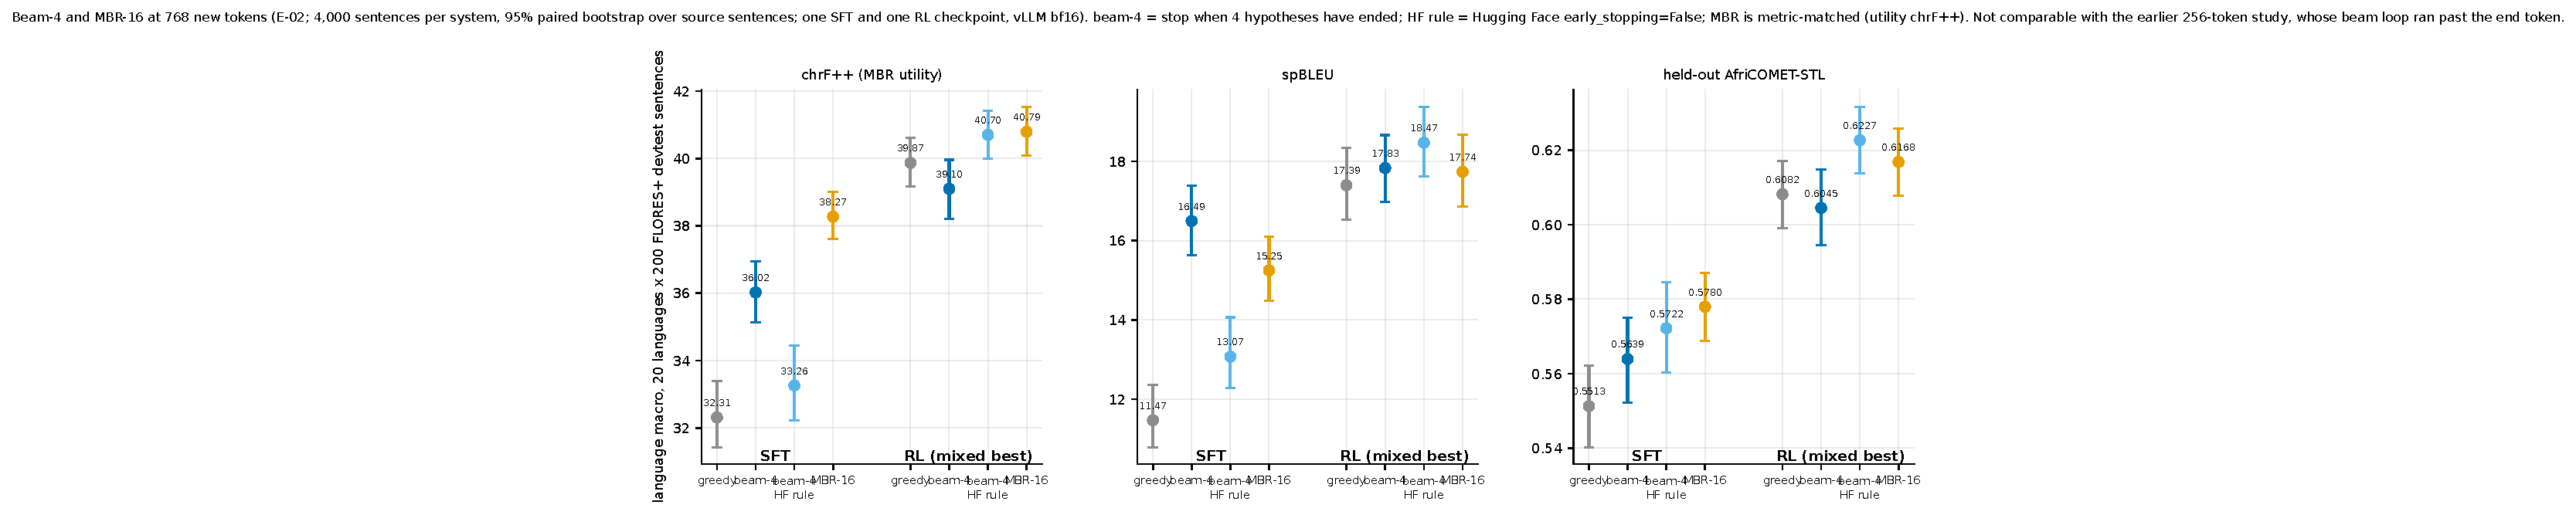
\includegraphics[width=1.00\linewidth,trim=384bp 0 384bp 26bp,clip]{figures/fig15_e02_decoding.pdf}
\caption{Greedy, beam-4 and MBR-16 at 768 new tokens (E-02) for the SFT and the RL model (mixed best): chrF++, spBLEU and held-out AfriCOMET-STL, language macro over 20 languages $\times$ 200 FLORES+ devtest sentences (4,000 per system), 95\% paired bootstrap over source sentences; beam-4 stops when 4 hypotheses have ended, the HF rule is early\_stopping=False, MBR is metric-matched (utility chrF++). One SFT and one RL checkpoint, vLLM bf16. Not comparable with the earlier 256-token study. Source: \texttt{reports/\allowbreak{}data/\allowbreak{}e02\_\allowbreak{}beam\_\allowbreak{}mbr\_\allowbreak{}768\_\allowbreak{}2026-\allowbreak{}11-\allowbreak{}05/\allowbreak{}cmp\_\allowbreak{}all.\allowbreak{}json}.}\label{fig:decoding_app}
\end{figure}

\begin{figure}[t]
\centering
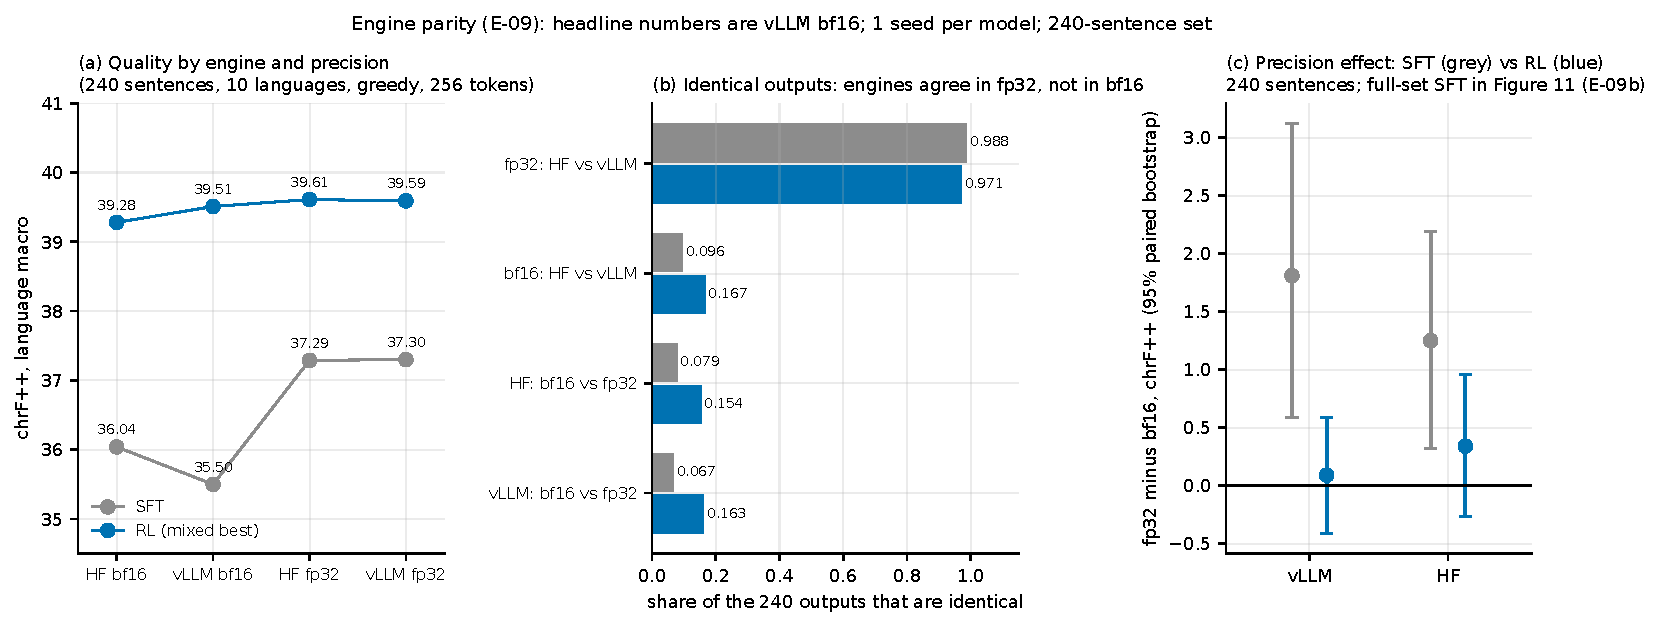
\includegraphics[width=1.00\linewidth]{figures/fig8_engine_parity.pdf}
\caption{Engine parity (E-09), 240 sentences (10 languages $\times$ 24 FLORES+ devtest sentences), greedy, 256 new tokens, SFT and RL (mixed best), one seed. (a) Language-macro chrF++ by engine and precision. (b) Share of identical outputs: vLLM and HF agree in fp32 (0.988, 0.971) and not in bf16 (0.096, 0.167). (c) fp32 minus bf16 chrF++ with 95\% paired bootstrap over sentences: negligible for the RL model, +1.81 [+0.59, +3.12] (vLLM) for the SFT on this small set, which the full-set run of Figure 11 does not reproduce. Headline numbers of the paper are vLLM bf16. Sources: \texttt{reports/\allowbreak{}data/\allowbreak{}e09\_\allowbreak{}engine\_\allowbreak{}parity\_\allowbreak{}2026-\allowbreak{}11-\allowbreak{}04/\allowbreak{}\{parity\_\allowbreak{}bootstrap,parity\_\allowbreak{}summary\}.\allowbreak{}json}.}\label{fig:fig8_engine_parity}
\end{figure}

\begin{figure}[t]
\centering
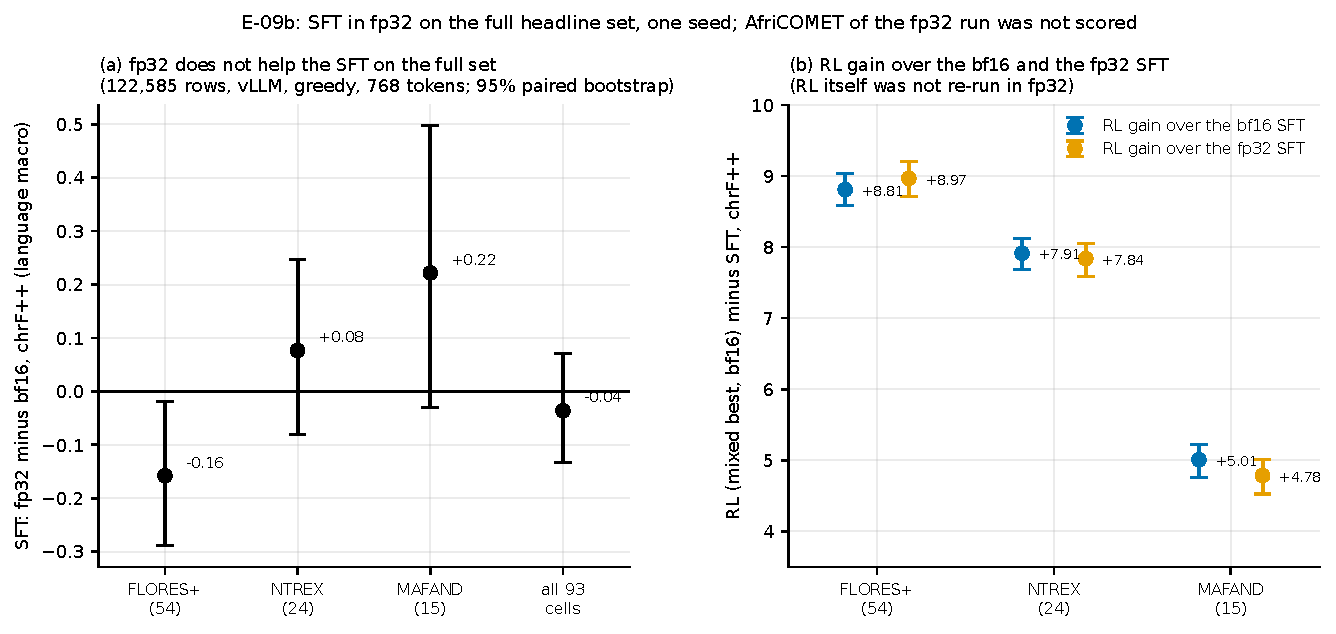
\includegraphics[width=0.90\linewidth]{figures/fig11_fp32_full_set.pdf}
\caption{Full-set precision check (E-09b): the SFT generated in fp32 instead of bf16 (vLLM, greedy, 768 new tokens, 122,585 rows, 214 flagged rows removed; one seed). (a) fp32 minus bf16 chrF++ (language macro, 95\% paired bootstrap over sentences) on FLORES+ (54 languages), NTREX (24), MAFAND (15) and over all 93 cells (\ensuremath{-}0.04 [\ensuremath{-}0.13, +0.07]). (b) RL gain (mixed best, bf16) over the bf16 SFT and over the fp32 SFT. The RL model was not re-run in fp32 and the AfriCOMET of the fp32 run was not scored. Source: \texttt{reports/\allowbreak{}data/\allowbreak{}e09b\_\allowbreak{}fp32\_\allowbreak{}2026-\allowbreak{}11-\allowbreak{}04/\allowbreak{}evidence\_\allowbreak{}e09b.\allowbreak{}json}.}\label{fig:fig11_fp32_full_set}
\end{figure}

\section{NLLB comparison and other systems: details}\label{app:afrique}

The RL closes 74\% of the gap between the SFT and NLLB-3.3B (12.50 $\to$ 3.26; arithmetic of the two differences), and stage A alone gives 8.61 of the 9.24 chrF++ that the mixed best adds over the SFT on these languages (93\%). The remaining gap is not a finishing or looping artefact: on these 43 languages the mixed best finishes at least 0.99 and repeats at most 0.02 in every language. By NLLB-3.3B tertile (14 / 14 / 15 languages) the mixed best reaches 91.7\% (high, 46.82 against 51.05), 87.7\% (mid, 34.57 against 39.42) and 96.8\% (tail, 25.92 against 26.78) of NLLB-3.3B; the SFT 75.3\%, 63.2\% and 60.7\%. The mixed best matches or beats NLLB-3.3B on 7 of 43 languages, all in the lowest tertile (yor +5.43, fon +2.95, dyu +2.77, wol +2.48, kam +2.32, kmb +2.22, umb +1.86; the SFT only on fon, 20.17 against 19.30) and is within 1 chrF++ on 9. The largest remaining gaps are amh \ensuremath{-}11.28, kin \ensuremath{-}9.74, kea \ensuremath{-}8.72, run \ensuremath{-}8.02, ewe \ensuremath{-}7.03, lug \ensuremath{-}6.77, tir \ensuremath{-}6.06 and hau \ensuremath{-}6.04. 
% src: NLLBRL sections 0, 2, 3 (`table3_by_nllb_tertile.csv`, `table2_per_language_43.csv`)

\textbf{Same sentences.} In the post-editor run, NLLB-3.3B and RL stage A drafts were scored on identical 100-sentence FLORES+ subsets (language bootstrap only; sentence hypotheses are not stored). With beam-4 on our side (the beam setup of the post-editor run, not that of E-02) and NLLB greedy on theirs, stage A is 1.44 below NLLB-3.3B on 43 languages (36.12 against 37.56, [\ensuremath{-}2.34, \ensuremath{-}0.56]; 13 languages at least equal) and 3.67 below on all 50 languages both have; held-out AfriCOMET 0.6414 against 0.6709 (\ensuremath{-}0.0294 [\ensuremath{-}0.0366, \ensuremath{-}0.0222], 40 languages, ahead in 5). Our own NLLB run on 100 sentences is 1.23 [\ensuremath{-}1.60, \ensuremath{-}0.86] below the published full-devtest value, which bounds the sample and reference effects. AfriCOMET is the QE reward's family, so that row is not independent evidence for the RL model. 
% src: NLLBRL section 4 (`table6b_same_sentence_summary.csv`, `table7_africomet_same_100_sentences.csv`)

\textbf{AfriqueLLM family, indicative only.} On the 21 languages with per-language values in the 5-shot AfroBench-Lite harness (afr amh ewe hau ibo kin lin lug nya orm sna som sot swh tir tsn twi wol xho yor zul): SFT 32.37, stage A 39.13, B1 best 39.32, mixed best 39.40, weak final 39.26, against AfriqueQwen3.5-4B-50Langs 41.71 (mixed best \ensuremath{-}2.31; ahead in 4 of 21 languages), AfriqueGemma-12B 38.58 (+0.83; 6 of 21), AfriqueLlama-8B 36.71, AfriqueQwen-14B 36.67, AfriqueQwen-8B 35.06, AfriqueGemma-4B 31.12, Gemma3-12B 18.82, Llama3.1-8B 16.45. Those are base models in 5-shot prompting with a harness whose chrF++ implementation and FLORES split are not verified.   Bidirectional aggregates (TranslatePsy, AfriNLLB) and pooled AfroBench rows are not comparable and are not compared.
% src: NLLBRL section 5 `table5_afrique_21_languages.csv`; ledger N3 status weak

\section{Family, script and resource level (exploratory, fragile)}\label{app:family}

We labelled all 125 registry languages with Glottolog 5.3 \citep{glottolog53} (CLDF release v5.3, commit 072ca0d of glottolog-cldf, CC BY 4.0, Zenodo 10.5281/zenodo.18840967) and asked whether the RL gain (mixed best minus SFT, FLORES+ devtest chrF++, 54 languages) depends on family, script or resource level. \textbf{This analysis is observational, has 54 languages in 7 families, several with 1 to 3 members, and its main result changes with the languages included. We report it as description, not as a finding.} 
% src: FAMILY sections 0, 3-5

\begin{table}[t]
\centering\scriptsize
\setlength{\tabcolsep}{4pt}
\caption{RL gain (mixed best minus SFT, FLORES+ devtest \chrfpp{}, 54 languages) by Glottolog family, script and regression family; bootstrap over languages.}\label{tab:family}
\begin{tabularx}{\linewidth}{@{}l>{\raggedright\arraybackslash}Xrr>{\raggedright\arraybackslash}X@{}}
\toprule
grouping & group & n & mean SFT chrF++ & mean gain [bootstrap CI over languages] \\
\midrule
Glottolog top family & Atlantic-Congo & 33 & 26.20 & +9.14 [+7.58, +10.79] \\
 & Afro-Asiatic & 11 & 13.45 & +6.89 [+4.29, +9.89] \\
 & Nilotic & 3 & 12.87 & +11.58 [+10.30, +13.13] \\
 & Indo-European (creoles, Afrikaans) & 3 & 36.85 & +10.23 [+1.01, +20.27] \\
 & Mande & 2 & 14.65 & +8.42 [+7.78, +9.06] \\
regression family & Narrow Bantu & 24 & 27.36 & +9.91 [+7.96, +11.71] \\
 & other Atlantic-Congo & 9 & 23.11 & +7.06 [+4.76, +9.61] \\
script & Latin & 48 & 24.84 & +9.32 [+8.03, +10.68] \\
 & Ethiopic (amh tir) & 2 & 13.55 & +9.13 [+8.26, +10.00] \\
 & Arabic (aeb ary arz) & 3 & 4.00 & +2.73 [+1.36, +4.59] \\
 & Tifinagh (zgh) & 1 & 2.29 & +1.78 \\
\bottomrule
\end{tabularx}
\end{table}

(Single-language groups, Saharan knc and Austronesian mlg, are in the report. Glottolog's Nilotic group differs from the earlier ``Nilo-Saharan'' group of EVID Table 4 by dik versus knc, which is why the two means agree, +11.58 and +11.62.)

\begin{itemize}
\item The lowest gains are the Arabic-script dialects and Tifinagh, the languages where the SFT's output was English, Arabic or loops and the RL did not repair it (Section~\ref{sec:rlsft}). The eight languages that lacked a family label are now labelled: aeb, ary and arz Afro-Asiatic (Semitic, Arabic script), taq and zgh Afro-Asiatic (Berber), cjk Narrow Bantu, dik Nilotic, mfe French-lexifier creole. 
% src: FAMILY section 2 (`unlabelled8_labels.csv`)
\item \textbf{The gain is not explained by the token budget} (Spearman rho(gain, log10 SFT tokens) = \ensuremath{-}0.16 [\ensuremath{-}0.44, +0.13], n = 54; OLS slope +0.34 chrF++ per log10 unit [\ensuremath{-}2.03, +1.79], R2 0.003), while the SFT level is (rho = +0.68 [+0.47, +0.82]; slope +11.8 [+8.5, +17.0], R2 0.45). \textbf{This is fragile:} dropping Afro-Asiatic turns the slope on the gain from +0.34 into \ensuremath{-}3.00 (SE 1.06), so ``no relation'' depends on which languages are in the sample. What the gain does track is the SFT's failure rate (rho with the SFT finished rate \ensuremath{-}0.47 [\ensuremath{-}0.74, \ensuremath{-}0.15], with its repeat rate +0.46 [+0.13, +0.72], n = 54 each), in line with Section~\ref{sec:rlsft}: family, script and resource effects on the raw gain are largely effects on how badly the SFT failed.
\item A regression of the gain on family, log tokens, non-Latin script, AfriCOMET availability and NLLB-mined share (n = 53, 11 parameters) explains little (R2 0.27, adjusted 0.09). Only non-Bantu against Narrow Bantu Atlantic-Congo is clearly non-zero (\ensuremath{-}4.45 [\ensuremath{-}8.36, \ensuremath{-}1.24], robust p = 0.020, uncorrected for the many contrasts); the NLLB-mined share is positive (+7.57 [+0.91, +14.67], p = 0.066), which reflects that NLLB-dependent languages are the low-resource tail that started low and failed by loops; it does not say whether NLLB data helped or hurt (Appendix~\ref{app:nllblink}). The same model explains most of the SFT level (R2 0.67, adjusted 0.59). Family, script, tokens, resource tier and AfriCOMET availability overlap (VIF 2.1 to 3.4), and three of six mixed-model fits did not converge.
\item Only 54 of 125 languages (58 with NTREX and MAFAND) have a gain; 51 have no reference test, so no family or script statement is possible for them. The 54 are the better-resourced languages (median 25.4 M tokens against 8.6 M for the Latin-script registry). The token table is provisional, the script of 51 languages is assigned from prior knowledge, and the analysis was run after the results were known.
\end{itemize}

\section{Science and document results: details}\label{app:docs}

Start: the mixed-stage best. Science SFT: AdamW 3e-6, 283 steps of 65,536 tokens (6.34 M AfriScience tokens in 6 languages, two passes, plus 12.19 M replay tokens), AfriScience dev loss 1.699 $\to$ 1.322. The SFT end point (alpha 1.0) loses 2.45 NTREX and 1.20 MAFAND chrF++, so the weights were interpolated, theta(alpha) = (1 - alpha) theta\_start + alpha theta\_science, with a rule fixed beforehand (best AfriScience dev chrF subject to NTREX and MAFAND not more than 0.5 below the start); alpha = 0.5 was chosen. 
% src: reports/eval_science_sft_385m_2026-11-04.md

\begin{table}[t]
\centering\footnotesize
\setlength{\tabcolsep}{4pt}
\caption{Weight interpolation sweep of the science SFT, AfriScience-MT test (macro over six languages), with NTREX and MAFAND-MT \chrfpp{} (last two columns). SSA-QE = SSA-COMET-QE (headline); AfriC. = AfriCOMET-STL.}\label{tab:alpha}
\begin{tabular}{@{}rrrrrrrrr@{}}
\toprule
$\alpha$ & SSA-QE & chrF & chrF++ & BLEU & spBLEU & AfriC. & NTREX & MAFAND \\
\midrule
0 & 0.6130 & 45.40 & 42.44 & 17.72 & 21.89 & 0.6828 & 37.16 & 40.78 \\
0.3 & 0.6128 & 46.28 & 43.40 & 18.73 & 23.25 & 0.6865 & 37.13 & 41.06 \\
0.5 (chosen) & 0.6118 & 46.63 & 43.80 & 19.27 & 23.87 & 0.6879 & 36.90 & 41.05 \\
0.7 & 0.6092 & 46.56 & 43.81 & 18.98 & 23.83 & 0.6859 & 36.43 & 40.83 \\
1.0 & 0.5986 & 44.92 & 42.30 & 16.78 & 20.87 & 0.6708 & 34.71 & 39.58 \\
\bottomrule
\end{tabular}
\end{table}

\textbf{The science SFT gives surface gains (chrF +1.2, BLEU +1.5, spBLEU +2.0 at alpha 0.5) and no SSA-COMET-QE gain} (dev 0.6242 against 0.6235). SSA-COMET-QE here is the reference-free \texttt{McGill-\allowbreak{}NLP/\allowbreak{}ssa-\allowbreak{}comet-\allowbreak{}qe}, the variant that reproduces the AfriScience-MT paper's released values (mean absolute difference 0.006 over the six strongest released runs, 0.031 over nine); there is no RL in this comparison, so it is independent of the reward.  The metric choice was made after the alpha rule (Appendix~\ref{app:disc}). The 385M with the science SFT is below the old 270M science-stage models on AfriScience test chrF (46.6 against 47.9 for the old RL-final, 50.0 and 50.2 for the old science-stage models) and below the published fine-tuned NLLB-1.3B (52.3). 
% src: SCI alpha sweep; DOC calibration; HYG X13 (SCI's caveat paragraph is stale, quote DOC)
% src: SCI Table 2

\textbf{Science RL.} The run executed 160 steps (cap extended from 150 to 190 at step 120, stopped on a dev plateau at step 150 plus a 10-step wind-down; Appendix~\ref{app:chain}, ledger X24). Evaluation was fixed in advance: independent evidence = plain chrF on AfriScience-MT test and held-out AfriCOMET; SSA-COMET-QE and SSA-COMET-MTL are reward-family and shown but not counted. The final checkpoint is a small real sentence-level gain over its start (science SFT, alpha 0.5): chrF +0.46 [+0.27, +0.65] on AfriScience test and held-out AfriCOMET +0.0053 [+0.0036, +0.0071]; the step-75 \texttt{best} checkpoint is smaller (chrF +0.16 [\ensuremath{-}0.04, +0.37]); SSA-COMET-QE moves by +0.004 only; NTREX and MAFAND do not regress (chrF++ +0.42, +0.10). There is no document-level gain: chunked window SSA-COMET-QE is 0.574 (start), 0.574 (best), 0.577 (final), and the earlier 270M work's 270M models stay ahead on sentence chrF (47.9-50.2 stored numbers against 47.10) and on chunked documents (0.593 against 0.577). One run, one seed. Numbers: \texttt{reports/\allowbreak{}eval\_\allowbreak{}science\_\allowbreak{}rl\_\allowbreak{}385m\_\allowbreak{}2026-\allowbreak{}11-\allowbreak{}04.\allowbreak{}md}. \textbf{Disclosure:} the long-document RL start model was changed from \texttt{best} to \texttt{final} after this evaluation, including its test numbers (rule refined on the full AfriScience dev set, where final beats best by +0.24 chrF and +0.0031 AfriCOMET; the test split was not used for the rule); logged in \texttt{reports/\allowbreak{}overnight\_\allowbreak{}log\_\allowbreak{}2026-\allowbreak{}11-\allowbreak{}04.\allowbreak{}md}. SSA-COMET-QE, AfriCOMET and chrF for every stage are tabulated below (E-05). The RL-only science arm (mixed best to science RL without the science SFT) is reported next (E-14).

\textbf{Science RL without the science SFT (E-14).} To ask whether the science SFT is needed, the executed science RL was repeated with the start model changed to the mixed best (= science-SFT alpha 0, the model the science SFT was built from): same seed 1234, same pool, same reward, Muon at 1e-6, KL 0.1 against the start model, 160 steps (150 plus a 10-step wind-down), pre-declared checkpoint = final. The rule was registered before the run: the science SFT is \emph{not needed} if the lower 95\% bounds of E-14 minus the science RL final on AfriScience-MT test are above \ensuremath{-}0.5 chrF and above \ensuremath{-}0.004 held-out AfriCOMET; it is \emph{needed} if the upper bound of either is below its margin. 

\begin{table}[t]
\centering\footnotesize
\setlength{\tabcolsep}{4pt}
\caption{Science RL without the science SFT (E-14): AfriScience-MT test, sentence level, macro over 6 languages.}\label{tab:e14a}
\begin{tabularx}{\linewidth}{@{}>{\raggedright\arraybackslash}Xrrrr@{}}
\toprule
model & chrF & chrF++ & AfriCOMET-STL (held out) & SSA-COMET-QE (reward family) \\
\midrule
mixed best (= alpha 0; E-14's start) & 45.40 & 42.44 & 0.6828 & 0.6130 \\
B1 final (stage-B1 RL) & 45.45 & 42.50 & 0.6846 & 0.6141 \\
\textbf{E-14 final (science RL, no science SFT)} & \textbf{45.66} & 42.69 & \textbf{0.6850} & 0.6153 \\
science SFT alpha 0.5 & 46.63 & 43.80 & 0.6879 & 0.6118 \\
science RL final (from the science SFT) & 47.10 & 44.22 & 0.6932 & 0.6158 \\
\bottomrule
\end{tabularx}
\end{table}

\begin{table}[t]
\centering\footnotesize
\setlength{\tabcolsep}{4pt}
\caption{E-14 final minus X, 95\% bootstrap (independent weights per language).}\label{tab:e14b}
\begin{tabularx}{\linewidth}{@{}>{\raggedright\arraybackslash}Xll>{\raggedright\arraybackslash}X@{}}
\toprule
E-14 final minus & chrF & AfriCOMET-STL (held out) & SSA-COMET-QE (reward family) \\
\midrule
science RL final (from the science SFT) & \textbf{-1.44 [\ensuremath{-}1.61, \ensuremath{-}1.25]} & \textbf{-0.0082 [\ensuremath{-}0.0101, \ensuremath{-}0.0065]} & \ensuremath{-}0.0006 [\ensuremath{-}0.0018, +0.0007] \\
science SFT alpha 0.5 & \ensuremath{-}0.97 [\ensuremath{-}1.20, \ensuremath{-}0.75] & \ensuremath{-}0.0030 [\ensuremath{-}0.0050, \ensuremath{-}0.0009] & +0.0035 [+0.0022, +0.0047] \\
mixed best (its own start) & +0.26 [+0.12, +0.39] & +0.0022 [+0.0007, +0.0036] & +0.0023 [+0.0013, +0.0033] \\
B1 final & +0.21 [+0.07, +0.36] & +0.0004 [\ensuremath{-}0.0012, +0.0020] & +0.0012 [+0.0000, +0.0023] \\
\bottomrule
\end{tabularx}
\end{table}

\textbf{By the registered rule the science SFT is needed:} the upper bounds are \ensuremath{-}1.25 chrF and \ensuremath{-}0.0065 AfriCOMET, both below their margins, chrF is lower in all six languages (\ensuremath{-}0.72 to \ensuremath{-}2.70) and the dev split agrees (\ensuremath{-}1.63 [\ensuremath{-}1.81, \ensuremath{-}1.44]). The science gain is carried by the science SFT (+1.23 chrF at alpha 0.5), not by the science RL: the RL alone on top of the mixed best adds +0.26 chrF [+0.12, +0.39] (+0.0022 AfriCOMET), a gain of the size at which seed noise matters (E-04), against +0.46 for the RL on top of the science SFT. The trainer's dev chrF++ stayed flat (43.50 $\to$ 43.43) while the executed science RL rose from 44.62 to 45.13, and no \texttt{best/\allowbreak{}} checkpoint was written (the dev macro never rose by the trainer's 0.2 margin), so only the final exists. \textbf{Reward-family caveat:} SSA-COMET-QE rates E-14 level with the science RL final (\ensuremath{-}0.0006 [\ensuremath{-}0.0018, +0.0007]) and above alpha 0.5 (+0.0035), while chrF and held-out AfriCOMET rate it below both: the metric the RL optimises moved without a matching move in the independent metrics, so it is not evidence of quality here. On the general benchmarks (93 cells) E-14 is +0.13 chrF++ [+0.10, +0.15] over the mixed best (FLORES+ +0.17, NTREX +0.12, MAFAND 0.00) and +0.34 [+0.31, +0.36] over B1 final, with no regression on NTREX and MAFAND (+0.12 / 0.00 against the mixed best; the executed science RL final is higher on MAFAND by 0.36); at document level it does not change chunked chrF (57.30 against 57.29 for its start) and whole-document decoding still fails (finished 0.69, loop 0.82, chrF 25.6). Caveats: one seed; one crash (a CUDA out-of-memory in the COMET reward worker at about step 38; the launcher's ladder halved the micro-batch from 12,288 to 6,144 tokens and resumed from the step-20 checkpoint, replaying steps 21 to 38, which can differ from the first pass because vLLM sampling is not bit-reproducible); the comparison with the science RL final mixes the effect of the science SFT with its alpha 0.5 interpolation (a science SFT at alpha 1.0 followed by RL was not run); 160 steps only. 
% src: reports/e14_science_rl_without_science_sft_2026-11-05.md sections 0-3; reports/data/e14_science_rl_no_sft_2026-11-05/ (ledger E14 rows SC7, SC8)

\textbf{SSA-COMET-QE for every stage (E-05).} The stored AfriScience-MT sentence predictions of every stage were scored with \texttt{McGill-\allowbreak{}NLP/\allowbreak{}ssa-\allowbreak{}comet-\allowbreak{}qe}, held-out AfriCOMET-STL and plain chrF (test, macro over 6 languages). SSA-COMET-QE is 0.5686 for the SFT and 0.6118 (stage A), 0.6113 (B1 best), 0.6130 (mixed best), 0.6118 (science SFT alpha 0.5), 0.6135 / 0.6158 (science RL best / final) and 0.6158 / 0.6165 (long-document RL best / final) for the RL stages: the first RL stage adds +0.043 and every later stage at most +0.005 more. It is a reward-family metric for every RL row, so these numbers are not evidence of quality; chrF (36.00 for the SFT, 45.06 stage A, 45.40 mixed, 46.63 science SFT, 47.10 science RL final, 47.16 long-document RL) and held-out AfriCOMET-STL (0.6064, 0.6822, 0.6828, 0.6879, 0.6932, 0.6936) keep rising by small steps that SSA-COMET-QE does not register. Alpha 1.0 (the full science SFT) is the only row clearly worse (0.5986). One seed per stage; test-sentence bootstrap intervals of the differences are +/\ensuremath{-}0.001 to +/\ensuremath{-}0.002 (Section~\ref{sec:science} tables). The numbers are for sentence level and are not comparable with the AfriScience-MT paper's document-level table. 
% src: reports/e05_ssa_all_stages_2026-11-04.md; reports/data/e05_ssa_all_stages_2026-11-04/{tables.md,e05_all.json} (ledger SC6, P4)

168 test documents (28 papers $\times$ 6 languages), a document being the paper's plain-language summary rebuilt from sentences. Whole-document generation (greedy, 4,096 new tokens) fails for the 385M models and is worse after the science SFT: start finished 0.71, loop 0.86, chrF 22.8, tail coverage 0.27; science SFT finished 0.51, loop 0.86, chrF 24.9; the old 270M RL-final finished 0.70, loop 0.61, chrF 34.9. Sentence-by-sentence (``chunked'') decoding with best-of-4 repair fixes finishing for all three (finished 1.00, sentence coverage 1.000): 
% src: reports/eval_afriscience_document_level_2026-11-04.md Tables 1-3

\begin{table}[t]
\centering\footnotesize
\setlength{\tabcolsep}{4pt}
\caption{Chunked document decoding (sentence by sentence with best-of-4 repair), 168 test documents.}\label{tab:docs}
\begin{tabularx}{\linewidth}{@{}>{\raggedright\arraybackslash}Xrrrr@{}}
\toprule
model (chunked) & SSA-COMET-QE, 4-sentence windows & chrF & AfriCOMET window & BLEU \\
\midrule
385M start (alpha 0) & 0.574 & 57.3 & 0.687 & 20.0 \\
385M science SFT (alpha 0.5) & 0.574 & 58.8 & 0.692 & 22.0 \\
old 270M RL-final (earlier 270M work) & 0.593 & 59.3 & 0.703 & 22.5 \\
\bottomrule
\end{tabularx}
\end{table}

The earlier 270M work's 270M RL-final is as good as or better than the 385M at document level (+0.019 window SSA-COMET-QE, +0.011 AfriCOMET window, +0.5 to +2.0 chrF; better on hau, lug, nso, zul, worse on amh). The COMET encoders read 512 tokens, so a concatenated-document COMET only sees the start of a document; the window values are the honest ones. Window SSA-COMET-QE is reward-family for the old model (trained against a QE reward); chrF and AfriCOMET are the independent checks. For reference, the AfriScience-MT paper's best released document-level system (GPT-5.4) has SSA-COMET 0.519 and chrF 64.5 under document handling we cannot reproduce. Caveats: one seed, 28 papers per language, no bootstrap. None of the 385M RL stages trained on prompts above 256 source tokens before the long-document RL; production use is sentence by sentence.

\textbf{Long-document RL.} The stage started from the science RL final (step 160), ran the planned 80 steps (32 prompts per step, about 51\% long prompts of 512 to 2,048 source tokens, group 8, no guide, hold-out-reward checkpoint selection, LibreTexts-free pool) and was evaluated at its best (step 50) and final (step 80) checkpoints on the same 168 documents. In whole-document mode, best against its start: finished \textbf{0.70 $\to$ 0.82 (+0.125 [+0.046, +0.204])}, loop rate \textbf{0.85 $\to$ 0.73 (\ensuremath{-}0.113 [\ensuremath{-}0.179, \ensuremath{-}0.056])}, chrF \textbf{27.4 $\to$ 30.9 (+3.4 [+1.5, +5.3])}, tail coverage 0.32 $\to$ 0.36 (95\% bootstrap over documents). The final checkpoint is similar (finished 0.85, loop 0.72, chrF 29.7, +2.2 [+0.4, +4.2], length ratio 0.81); best and final do not differ significantly (chrF \ensuremath{-}1.2 [\ensuremath{-}3.0, +0.7]). \textbf{Whole-document decoding remains unusable:} 15 to 18\% of the documents do not finish, 72 to 73\% show a repetition loop, and the output covers 34 to 36\% of the last third of the paper (chunked: 63\%). Chunked and sentence-level results do not change: window SSA-COMET-QE (reward family) 0.577 $\to$ 0.579 and 0.579 (a corpus-level number, no interval; a 0.002 difference is not an effect), chunked chrF 58.7 $\to$ 58.9 / 58.8 (best +0.13 [+0.04, +0.22]); AfriScience test sentences chrF 47.10 $\to$ 47.16 (+0.06 [\ensuremath{-}0.09, +0.20]), held-out AfriCOMET +0.0001 / +0.0004 with intervals around zero; NTREX / MAFAND chrF++ 37.33 / 41.14 $\to$ 37.43 / 41.15 (best). The earlier 270M work's 270M RL-final is still ahead in chunked mode (window SSA-COMET-QE 0.593 against 0.579) and in whole-document chrF (34.9 against 30.9). The effect is real but moderate and of the size of the other late-stage steps; the hold-out loop rate fell by only 2 points over the 80 steps, and the selection reward is the optimised quantity. One seed; 168 documents from 28 papers, so the intervals reflect paper sampling only. 
% src: reports/eval_long_document_rl_385m_2026-11-04.md sections 0-3 (LDOLR); reports/data/eval_long_rl_2026-11-04/{doc_tables.md,doc_pairs.json,sci_pairs_long.json}; ledger DL5, P2. The report says "best/ vs final/ indistinguishable"; wall-clock and crash loop in Section 15

\subsection{Figures for the science and document results}\label{app:figs}

\begin{figure}[t]
\centering
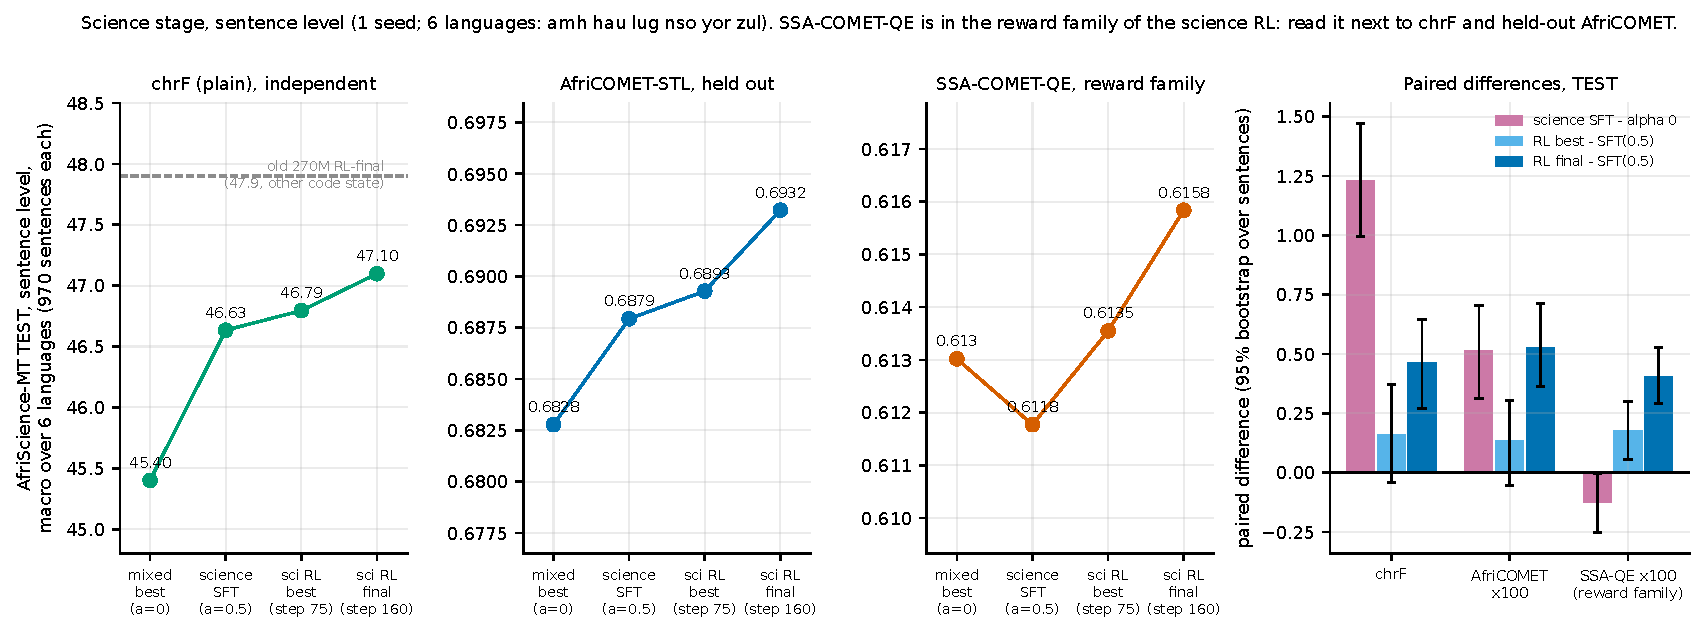
\includegraphics[width=1.00\linewidth]{figures/fig5a_science_sentence.pdf}
\caption{Science stage, AfriScience-MT TEST, sentence level (970 sentences per language, macro over amh hau lug nso yor zul; greedy; one seed): plain chrF (independent of the reward; dashed: the earlier 270M work's 270M RL-final, other code state), held-out AfriCOMET-STL (independent), and SSA-COMET-QE (reward family of the science RL) for the mixed best (alpha 0), the science SFT (alpha 0.5), and the science RL best (step 75) and final (step 160); right: paired differences with 95\% bootstrap over sentences. Sources: \texttt{reports/\allowbreak{}data/\allowbreak{}eval\_\allowbreak{}science\_\allowbreak{}rl\_\allowbreak{}2026-\allowbreak{}11-\allowbreak{}04/\allowbreak{}sci\_\allowbreak{}pairs.\allowbreak{}json}, \texttt{reports/\allowbreak{}data/\allowbreak{}eval\_\allowbreak{}science\_\allowbreak{}sft\_\allowbreak{}2026-\allowbreak{}11-\allowbreak{}04/\allowbreak{}tables.\allowbreak{}md}.}\label{fig:fig5a_science_sentence}
\end{figure}

\begin{figure}[t]
\centering
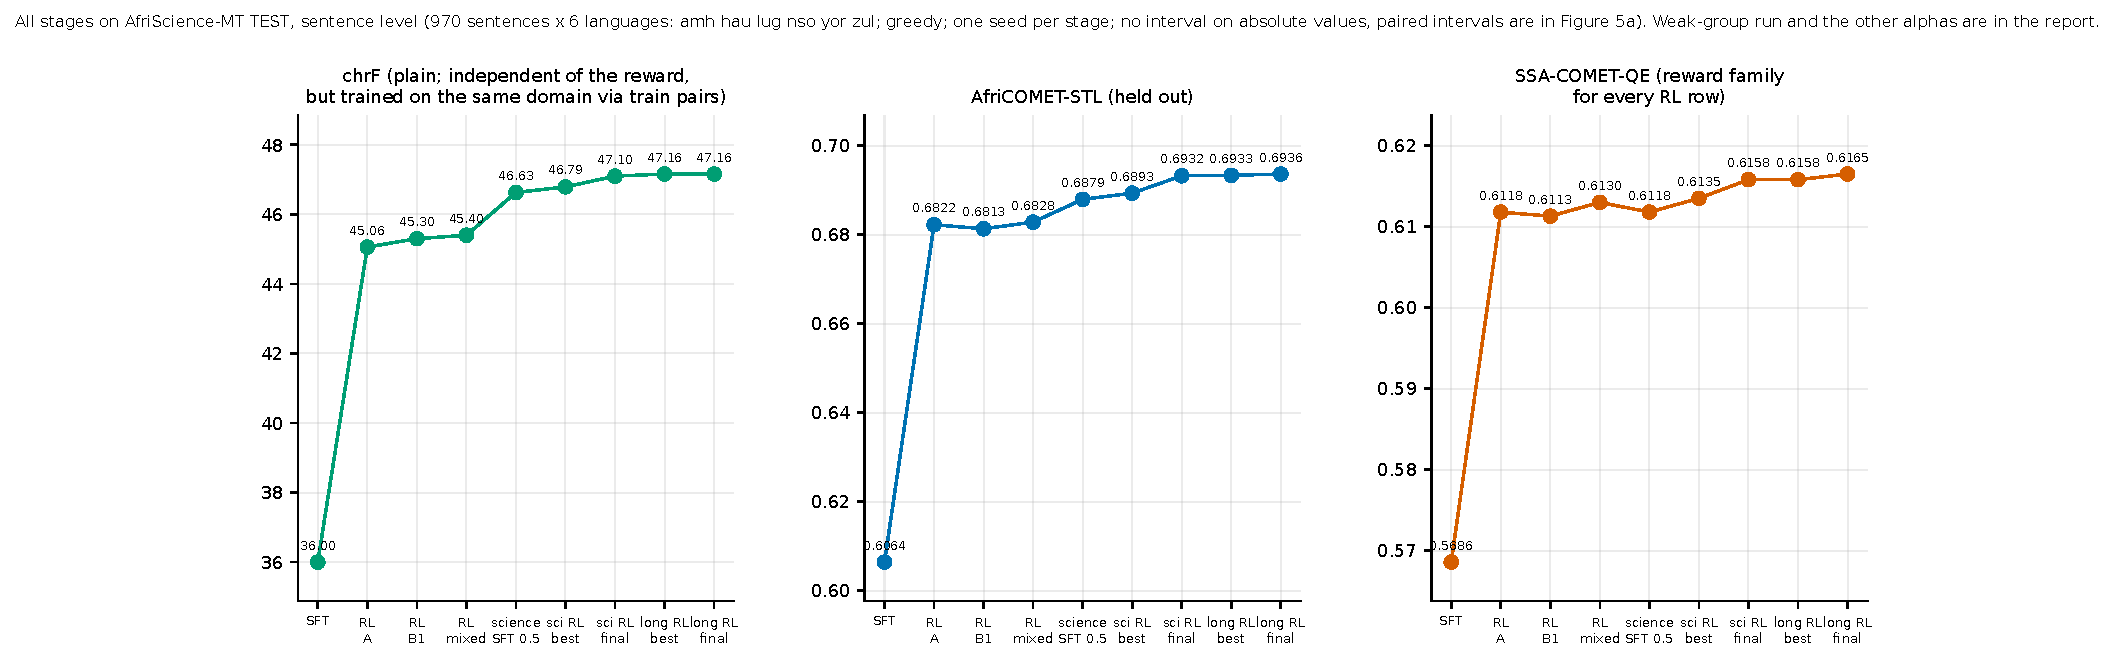
\includegraphics[width=1.00\linewidth]{figures/fig12_ssa_all_stages.pdf}
\caption{All stages on AfriScience-MT TEST, sentence level (970 sentences per language, macro over amh hau lug nso yor zul; greedy; one seed per stage): plain chrF, held-out AfriCOMET-STL and SSA-COMET-QE (reward family for every RL row) for the SFT, RL stages A, B1 and mixed, the science SFT (alpha 0.5), the science RL and the long-document RL. The weak-group run and the other interpolation weights are in the source table. Source: \texttt{reports/\allowbreak{}data/\allowbreak{}e05\_\allowbreak{}ssa\_\allowbreak{}all\_\allowbreak{}stages\_\allowbreak{}2026-\allowbreak{}11-\allowbreak{}04/\allowbreak{}tables.\allowbreak{}md}.}\label{fig:fig12_ssa_all_stages}
\end{figure}

\begin{figure}[t]
\centering
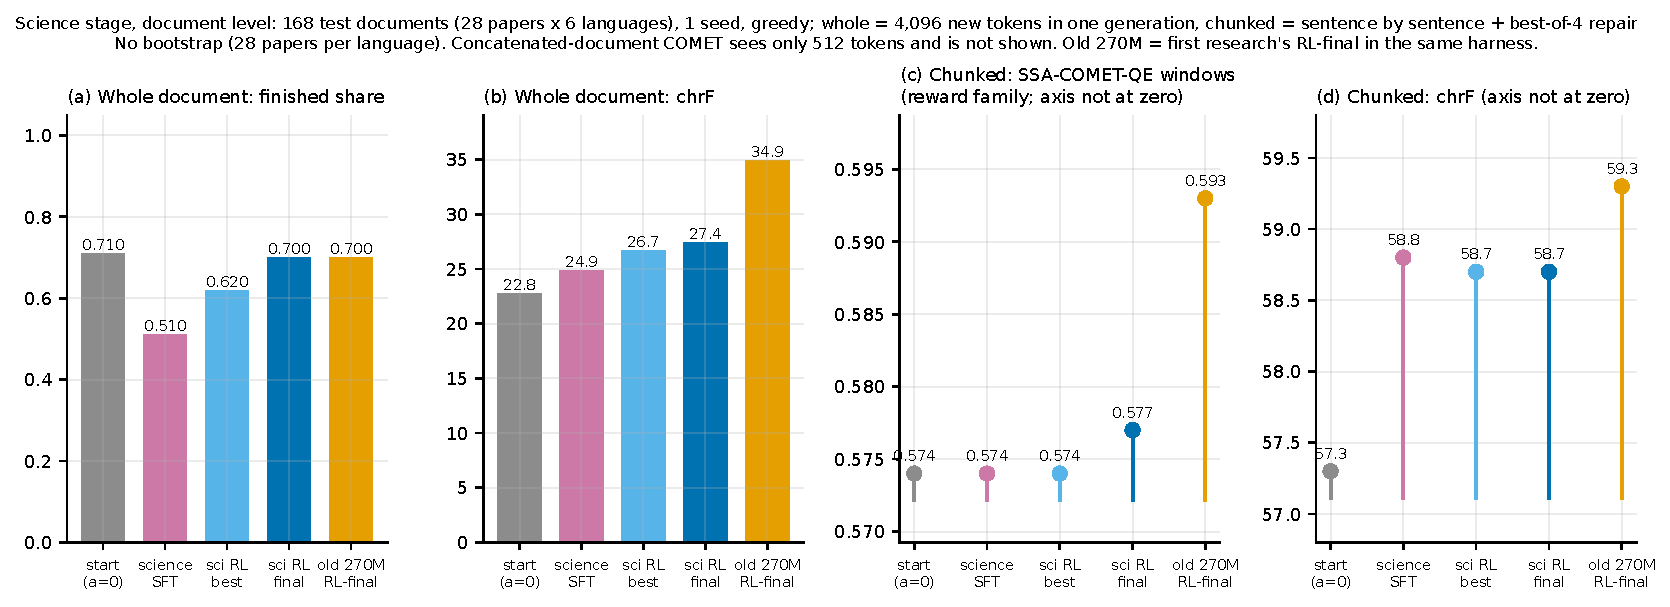
\includegraphics[width=1.00\linewidth]{figures/fig5b_science_document.pdf}
\caption{Science stage, document level: 168 test documents (28 papers $\times$ 6 languages), greedy, one seed, no bootstrap. Whole-document generation (4,096 new tokens): finished share and chrF. Chunked decoding (sentence by sentence plus best-of-4 repair): SSA-COMET-QE on 4-sentence windows (reward family) and chrF; axes of (c) and (d) do not start at zero. Source: \texttt{reports/\allowbreak{}data/\allowbreak{}eval\_\allowbreak{}science\_\allowbreak{}rl\_\allowbreak{}2026-\allowbreak{}11-\allowbreak{}04/\allowbreak{}doc\_\allowbreak{}tables.\allowbreak{}md}.}\label{fig:fig5b_science_document}
\end{figure}

\begin{figure}[t]
\centering
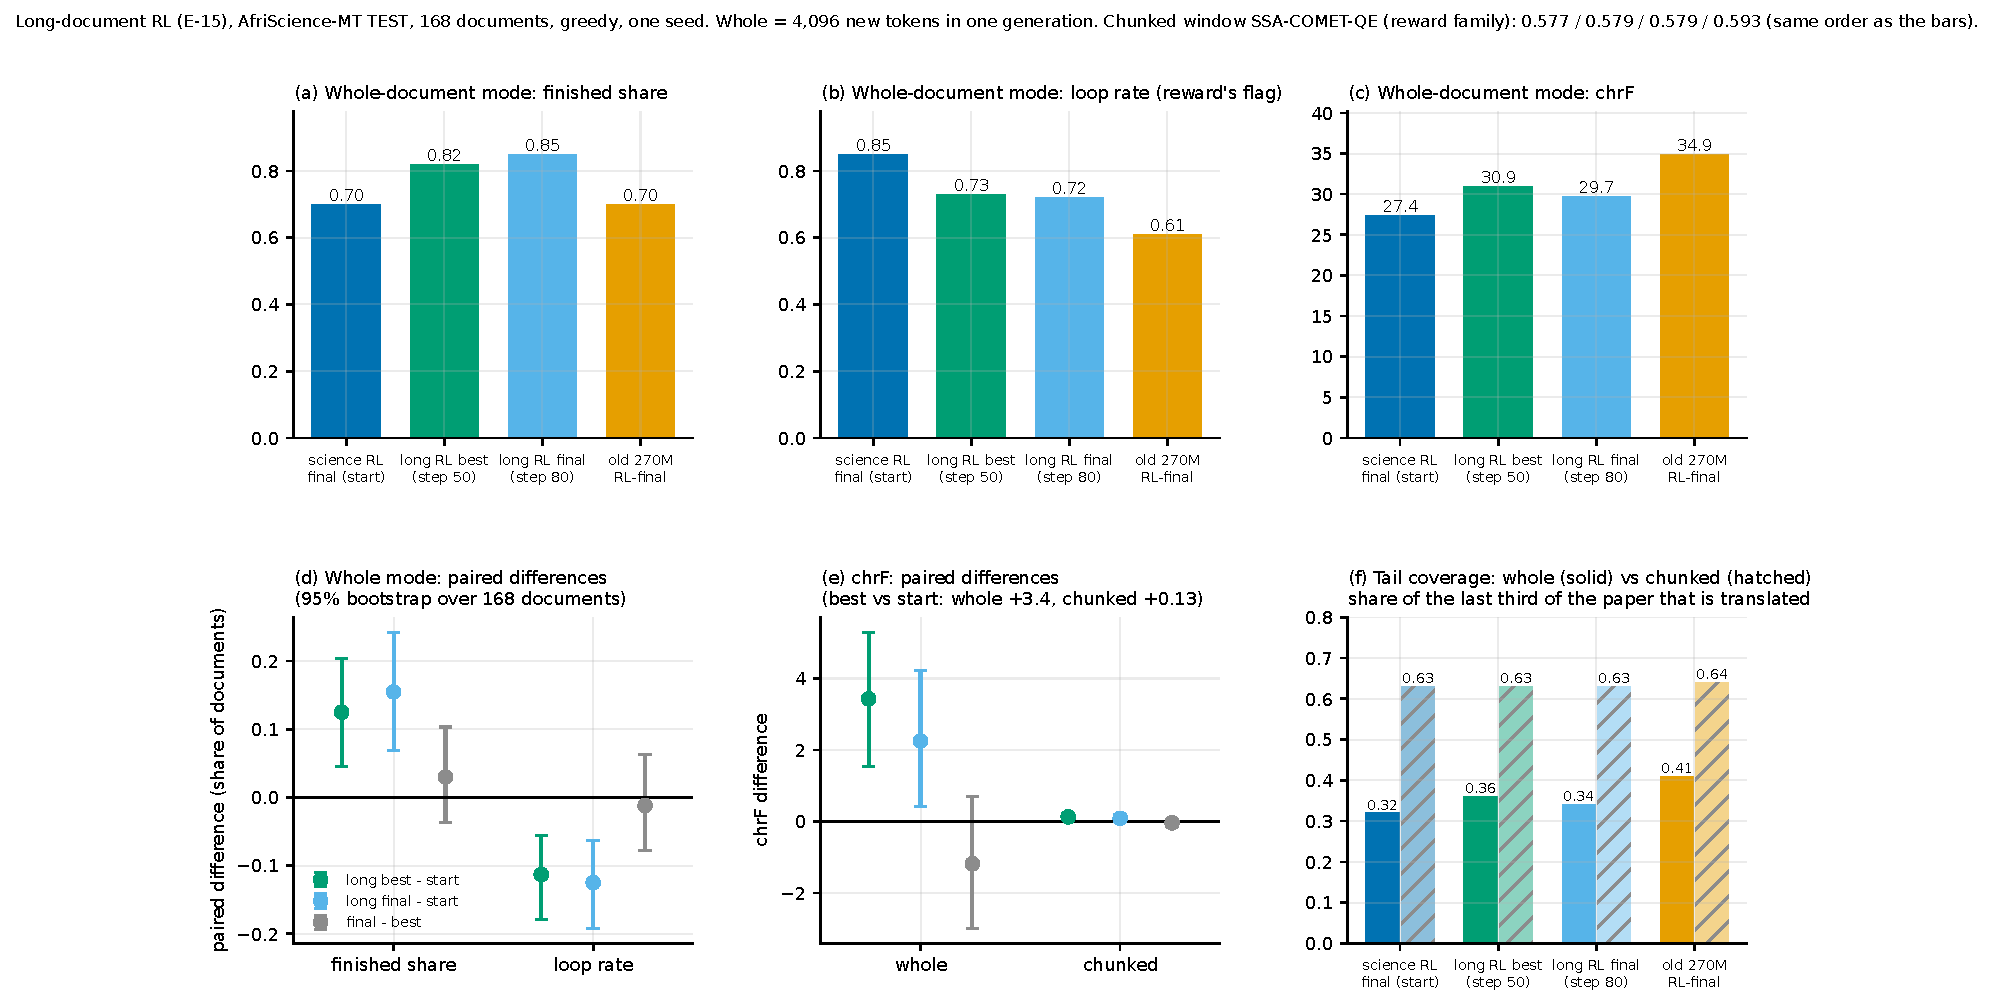
\includegraphics[width=1.00\linewidth]{figures/fig9_long_document_rl.pdf}
\caption{Long-document RL (E-15), AfriScience-MT TEST, 168 documents (28 papers $\times$ 6 languages), greedy, one seed. (a-c) Whole-document mode (4,096 new tokens in one generation): finished share, loop rate (the reward's flag) and chrF for the science RL final (the start), the long-document RL best (step 50) and final (step 80), and the earlier 270M work's 270M RL-final. (d, e) Paired differences with 95\% bootstrap over documents (Poisson weights): finished share, loop rate and chrF in whole mode, chrF in chunked mode. (f) Tail coverage, the share of the last third of the paper that is translated, whole against chunked mode. Chunked window SSA-COMET-QE (reward family) is in the figure title. Sources: \texttt{reports/\allowbreak{}data/\allowbreak{}eval\_\allowbreak{}long\_\allowbreak{}rl\_\allowbreak{}2026-\allowbreak{}11-\allowbreak{}04/\allowbreak{}\{doc\_\allowbreak{}tables.\allowbreak{}md,doc\_\allowbreak{}pairs.\allowbreak{}json\}}.}\label{fig:fig9_long_document_rl}
\end{figure}

\section{Contamination audit and follow-ups}\label{app:contam}

\textbf{6.4 Contamination.} The audit scanned both sides of 25,911,095 training samples (A0 packs and the six stage-B shards) against all benchmark rows: \textbf{no benchmark sentence of 3 or more words is in the training text}; FLORES+ devtest 0 of 54,648 rows, NTREX 120 of 47,928 (0.25\%), MAFAND 94 of 20,009 (0.47\%), SmolSent 45 of 38,833, GlotStoryBook 15 of 3,426, all one- or two-word strings; the FLORES+ dev train half is found in 23,706 of 23,760 rows (positive control); \texttt{all}, \texttt{clean}, \texttt{no\_\allowbreak{}pair} and \texttt{clean\_\allowbreak{}strict} macros agree within 0.01 chrF++. 
% src: reports/contamination_audit_385m_2026-11-03.md sections 1, 3, 6; reports/eval_385m_results_2026-11-03.md section 0

\emph{Follow-ups (CPU, 2026-11-04).} 
% src: CFU sections 0-6

\begin{itemize}
\item \textbf{Phrase level.} A lexical fuzzy scan of 56,975,939 pair rows and 4,277,612 instruction rows (reachable pair and instruction files, before gating and packing) finds no benchmark string of 8 or more tokens as a contiguous run. Strings of 4 to 7 tokens do occur inside longer training text (English side: MAFAND 134 of 17,428 strings, GlotStoryBook 30 of 898, NTREX 18 of 1,973, SALT 12 of 498; FLORES+ devtest, SmolSent, IbomMT and FLORES-MOZ 0); the audit's run rule and the intake filter test such short strings only for whole-sentence equality, so ``no benchmark sentence of 3 or more words'' holds for whole sentences, not for phrases. 263 (string, benchmark) cases of 8+ token English strings have a character-5-gram Jaccard $\ge$ 0.5 with some training text (MAFAND 184, SALT 27, NTREX 19, GlotStoryBook 15, SmolSent 6, FLORES+ devtest 4 of 1,012). These are candidates, not proof of leakage; their effect on scores was not measured.
\item \textbf{Prompts of the RL.} Stage A drew 6 flagged prompts of 28,120 (0.021\%); 6 of 1,345 prompts drawn for the seven languages whose prompt files had not been filtered (0.45\%), all distinct, in steps 72-364, source side only (this replaces the earlier estimate of about 0.15\%). The pool of the long-document RL (241,679 rows) has 0 rows flagged by the protected index.
\item \textbf{AfriScience-MT train versus the SFT text.} 305 of 34,007 train rows (0.9\%; hau 64, yor 116, zul 125) have their African-language sentence verbatim in the A0 pair data, all from \texttt{HuggingFaceFW/\allowbreak{}finetranslations}; 3 rows (yor 2, zul 1) as a pair. The packed shards were not scanned. The test papers are untouched (0 of 5,820 rows).
\item \textbf{A0 text.} The files support that A0's pack set is the first 138,873 packs of the audited g0 (identical per-language pack counts for 84 languages); pack content was not hash-compared.
\item \textbf{Not covered:} embedding or MT-round-trip paraphrase contamination, Gemma-3 pretraining, packed-shard coverage of the AfriScience train overlap and of the phrase scan (not run: these scans need the data box; Appendix~\ref{app:limits} item 15).
\end{itemize}

Benchmarks were evaluated many times; checkpoint choice used only the dev set (Appendix~\ref{app:limits}).

\section{NLLB-mined data and the regression against the earlier 270M work}\label{app:nllblink}

All 17 languages more than 5 chrF++ below the old SFT were already below with A0 (no NLLB-mined rows); the mean gap old SFT to A0 is \ensuremath{-}10.7 and A0 to 385M SFT +2.1; Venda (no NLLB rows) regressed \ensuremath{-}9.7. Spearman of NLLB share with the regression: \ensuremath{-}0.45 [\ensuremath{-}0.73, \ensuremath{-}0.09] on NTREX+MAFAND clean (n = 28), \ensuremath{-}0.07 [\ensuremath{-}0.35, +0.20] on the pooled index (n = 57), \ensuremath{-}0.17 [\ensuremath{-}0.54, +0.23] after RL. Each factor of 10 in NLLB-mined tokens adds \ensuremath{-}0.4 chrF++ (bootstrap 95\% [\ensuremath{-}11.0, +4.8]) against +9.6 for other new tokens. NLLB-mined rows are noisier than the same language's other rows (GlotLID acceptance median 0.77 against 0.99; AfriCOMET-QE below the language median in 38 of 43 languages). The decisive ablation (about 34 A100-hours) was not run [skipped by the authors; E-17]. The regression of Appendix~\ref{app:family} gives the same ambiguity: the NLLB-mined share is positively related to the RL gain and negatively to the SFT level, both through the low-resource tail. 
% src: reports/nllb_regression_link_2026-11-03.md; FAMILY section 4; the numbers of NLLBLINK were not independently re-run

\section{Negative results}\label{app:neg}

\begin{itemize}
\item Weak-group RL (Section~\ref{sec:seeds}), science SFT on the headline metric (Section~\ref{sec:science}), whole-document decoding (Section~\ref{sec:science}), RL on the Arabic dialects and Tamazight (outside the prompt pool; English output rises, Section~\ref{sec:degen}).
\item Post-editor: an SFT post-editor applied to every sentence lowers chrF++ (FLORES+ \ensuremath{-}0.01 [\ensuremath{-}0.11, +0.10], NTREX \ensuremath{-}0.58 [\ensuremath{-}0.75, \ensuremath{-}0.41], MAFAND \ensuremath{-}0.93 [\ensuremath{-}1.14, \ensuremath{-}0.74], SmolSent \ensuremath{-}0.37 [\ensuremath{-}0.52, \ensuremath{-}0.24]); restricted to the 3.9\% of drafts that are empty, unfinished or loops it gains +0.70 [+0.63, +0.78] chrF++ on FLORES+ but leaves AfriCOMET and SSA-COMET unchanged (\ensuremath{-}0.0007 to +0.0009), and beam-4 is stronger. 
% src: reports/post_editor_run_2026-11-03.md section 0
\end{itemize}

\section{Metric independence: full table}\label{app:indep}

\begin{table}[t]
\centering\footnotesize
\setlength{\tabcolsep}{4pt}
\caption{Metric independence (full). IND = not in any reward; RWD = in the reward; LOOP = optimised by construction.}\label{tab:indep_full}
\begin{tabularx}{\linewidth}{@{}>{\raggedright\arraybackslash}X>{\raggedright\arraybackslash}X>{\raggedright\arraybackslash}X@{}}
\toprule
metric & in the RL reward? & use in this paper \\
\midrule
\texttt{masakhane/\allowbreak{}africomet-\allowbreak{}qe-\allowbreak{}stl-\allowbreak{}1.\allowbreak{}1} (reference-free) & yes & not used as evidence \\
\texttt{McGill-\allowbreak{}NLP/\allowbreak{}ssa-\allowbreak{}comet-\allowbreak{}mtl} (reference-free; reference-based in the science RL) & yes & not used as evidence of RL gains \\
\texttt{McGill-\allowbreak{}NLP/\allowbreak{}ssa-\allowbreak{}comet-\allowbreak{}qe} (AfriScience-MT headline) & no, but the same family as the reward member & headline for SFT-only comparisons; for RL models shown only next to plain chrF and held-out AfriCOMET (all stages in Section~\ref{sec:science}) \\
TranslatePsy quality filters (AfriCOMET, SSA-COMET, MetricX) & not a reward; they filtered the training data of the E-03 control & neural metrics favour the control; chrF and chrF++ are the evidence (Section~\ref{sec:control}) \\
consensus utility (sample agreement in chrF++) & yes & chrF++ gains are partly in the optimised family \\
NLLB-3.3B pseudo-reference chrF++ & yes, 5 languages (kea kbp nus bam kab) & chrF++ on those 5 languages is not independent; relevant to the NLLB comparison (Section~\ref{sec:nllb}) \\
chrF++ against a human reference, weight 0.35 & yes, 7 languages (reference rows only; AfriScience TRAIN pairs) & chrF++ on those 7 languages can be partly trained; the test sets differ \\
language-ID, copy, repetition, length, end-of-turn guards & yes & finished and loop rates are optimised by construction \\
independent degeneration detector (lzma residual, repeated character 8-grams, repeated word 3-grams; thresholds from the 0.1\% tail of human references) & no & measures the same idea as the loop guard with different code and constants (Section~\ref{sec:rlsft}) \\
NLLB-218 language identification (\texttt{facebook/\allowbreak{}fasttext-\allowbreak{}language-\allowbreak{}identification}) & no & independent check of the language guard; evaluation use only (cc-by-nc-4.0) \\
\texttt{masakhane/\allowbreak{}africomet-\allowbreak{}stl-\allowbreak{}1.\allowbreak{}1} (reference-based) & no (held out; monitor and alarm) & the independent neural check; same family as the QE member \\
chrF / chrF++ / spBLEU against human references of the benchmarks & no & the main lexical evidence \\
\bottomrule
\end{tabularx}
\end{table}

% src: reports/rl_vs_sft_evidence_2026-11-04.md section 1; reports/eval_science_sft_385m_2026-11-04.md Goodhart caution; DEGEN section 1

\section{Per-language tables}\label{app:perlang}

\begin{figure}[t]
\centering
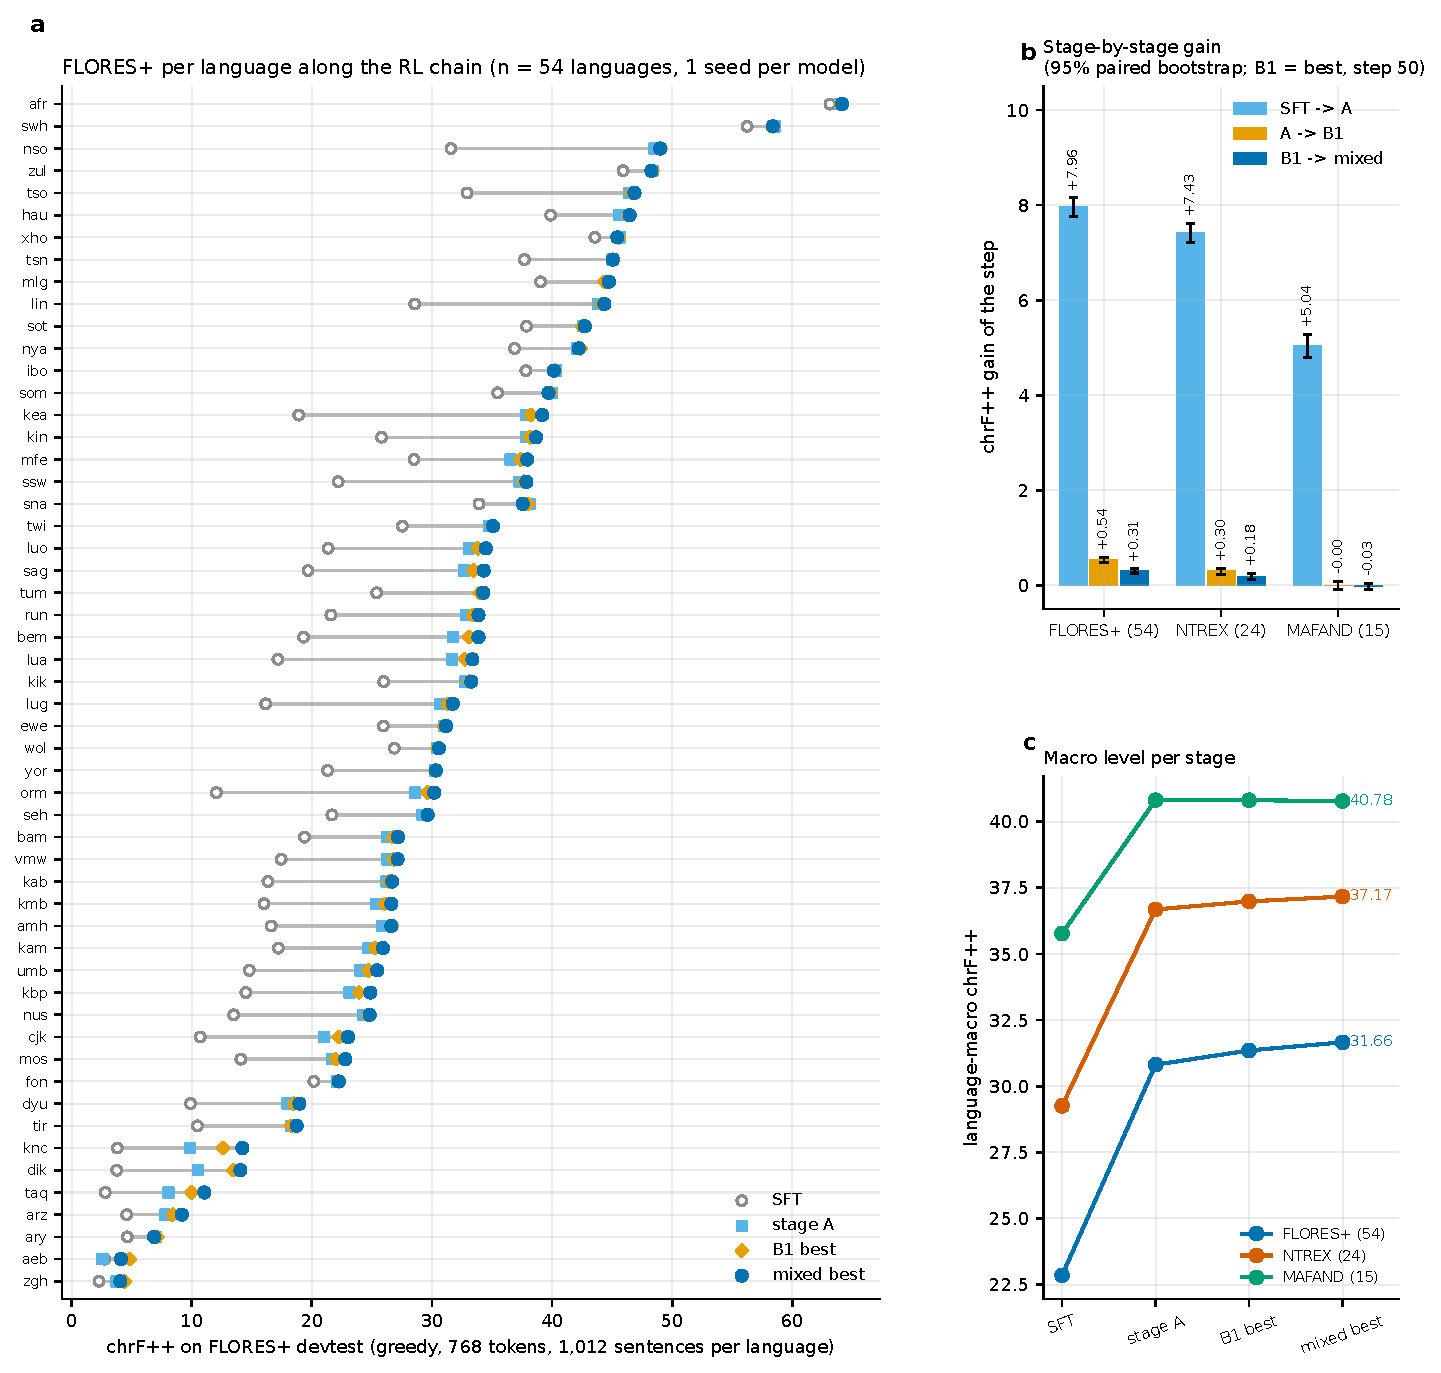
\includegraphics[width=0.95\linewidth]{figures/fig1_flores_per_language.pdf}
\caption{(a) FLORES+ devtest chrF++ per language (n = 54 languages, 1,012 sentences each; greedy, 768 tokens) for the SFT (open circle), RL stage A (square), B1 best (step 50, diamond) and the mixed best (filled circle), sorted by the mixed best; one training seed per model. (b) Gain of each RL step (language macro, 95\% paired bootstrap over sentences, Poisson weights shared across parallel languages) on FLORES+ (54 languages), NTREX (24) and MAFAND (15). (c) Language-macro chrF++ after each stage. Sources: \texttt{reports/\allowbreak{}data/\allowbreak{}eval\_\allowbreak{}weak\_\allowbreak{}group\_\allowbreak{}2026-\allowbreak{}11-\allowbreak{}03/\allowbreak{}results/\allowbreak{}results\_\allowbreak{}\{sft,stageA,b1best,mixedbest\}.\allowbreak{}csv}, \texttt{reports/\allowbreak{}data/\allowbreak{}rl\_\allowbreak{}vs\_\allowbreak{}sft\_\allowbreak{}evidence\_\allowbreak{}2026-\allowbreak{}11-\allowbreak{}04/\allowbreak{}evidence.\allowbreak{}json}.}\label{fig:fig1_flores_per_language}
\end{figure}

Sources: \texttt{reports/data/rl\_vs\_sft\_evidence\_2026-11-04/tables.md} (Tables 6, 7a, 7b) and \texttt{reports/data/nllb\_comparison\_rl\_models\_2026-11-04/table2\_per\_language\_43.csv}. Intervals are 95\% paired bootstrap over sentences (Poisson weights, 1,000 resamples); NLLB columns are published values.

{\scriptsize
\setlength{\tabcolsep}{4pt}
\begin{longtable}{@{}lrrllll@{}}
\caption{RL minus SFT per language on FLORES+ devtest (54 languages, all rows; \chrfpp{}). Finished / loop are the reward's flags; ``paired keeps rows where both models finished and neither loops.}\label{tab:perlang_flores}\\
\toprule
iso & SFT & RL & $\Delta$ all rows [CI] & SFT finished / loop & RL finished / loop & $\Delta$ paired rows [CI] \\
\midrule\endfirsthead
\toprule
iso & SFT & RL & $\Delta$ all rows [CI] & SFT finished / loop & RL finished / loop & $\Delta$ paired rows [CI] \\
\midrule\endhead
\bottomrule\endlastfoot
kea & 18.91 & 39.18 & +20.27 [+18.91, +21.53] & 0.83 / 0.20 & 1.00 / 0.00 & +7.66 [+6.93, +8.42] \\
orm & 12.06 & 30.18 & +18.12 [+17.49, +18.76] & 0.59 / 0.45 & 1.00 / 0.00 & +2.99 [+2.51, +3.50] \\
nso & 31.58 & 49.01 & +17.43 [+15.75, +19.09] & 0.86 / 0.15 & 1.00 / 0.00 & +4.22 [+3.62, +4.91] \\
lua & 17.18 & 33.37 & +16.19 [+15.21, +17.13] & 0.85 / 0.25 & 1.00 / 0.00 & +5.45 [+4.94, +6.03] \\
lin & 28.56 & 44.35 & +15.78 [+14.19, +17.22] & 0.90 / 0.13 & 1.00 / 0.00 & +5.27 [+4.69, +5.84] \\
ssw & 22.20 & 37.86 & +15.66 [+14.46, +16.85] & 0.87 / 0.17 & 1.00 / 0.00 & +5.38 [+4.85, +5.93] \\
lug & 16.17 & 31.73 & +15.57 [+14.66, +16.52] & 0.79 / 0.25 & 1.00 / 0.01 & +5.32 [+4.78, +5.87] \\
sag & 19.68 & 34.31 & +14.62 [+13.64, +15.55] & 0.87 / 0.20 & 1.00 / 0.00 & +5.99 [+5.51, +6.47] \\
bem & 19.31 & 33.88 & +14.56 [+13.63, +15.61] & 0.88 / 0.18 & 1.00 / 0.01 & +7.16 [+6.60, +7.75] \\
tso & 32.92 & 46.86 & +13.93 [+12.43, +15.51] & 0.91 / 0.11 & 1.00 / 0.00 & +4.45 [+3.82, +5.07] \\
luo & 21.36 & 34.49 & +13.13 [+11.91, +14.15] & 0.92 / 0.13 & 1.00 / 0.00 & +6.44 [+5.88, +6.95] \\
kin & 25.81 & 38.66 & +12.86 [+11.66, +14.03] & 0.89 / 0.12 & 1.00 / 0.00 & +5.66 [+5.09, +6.21] \\
cjk & 10.72 & 23.02 & +12.31 [+11.70, +12.89] & 0.71 / 0.31 & 1.00 / 0.01 & +2.13 [+1.86, +2.42] \\
run & 21.59 & 33.88 & +12.29 [+11.21, +13.15] & 0.88 / 0.15 & 1.00 / 0.01 & +5.03 [+4.52, +5.57] \\
nus & 13.49 & 24.82 & +11.32 [+10.73, +11.91] & 0.67 / 0.41 & 1.00 / 0.00 & +1.97 [+1.56, +2.36] \\
umb & 14.80 & 25.46 & +10.66 [+9.77, +11.44] & 0.89 / 0.15 & 1.00 / 0.01 & +4.84 [+4.43, +5.26] \\
kmb & 16.02 & 26.62 & +10.61 [+9.82, +11.37] & 0.88 / 0.23 & 1.00 / 0.00 & +3.93 [+3.56, +4.29] \\
knc & 3.81 & 14.22 & +10.41 [+9.95, +10.88] & 0.46 / 0.94 & 1.00 / 0.48 & +2.49 [+0.82, +3.99] \\
kbp & 14.51 & 24.88 & +10.37 [+9.70, +11.00] & 0.85 / 0.26 & 1.00 / 0.01 & +5.48 [+4.98, +5.94] \\
kab & 16.35 & 26.69 & +10.34 [+9.50, +11.14] & 0.84 / 0.20 & 1.00 / 0.00 & +2.26 [+1.92, +2.61] \\
dik & 3.76 & 14.06 & +10.30 [+9.75, +10.81] & 0.29 / 0.85 & 1.00 / 0.40 & +1.80 [+1.10, +2.60] \\
amh & 16.62 & 26.62 & +10.00 [+9.04, +10.96] & 0.87 / 0.13 & 1.00 / 0.00 & +2.80 [+2.29, +3.29] \\
vmw & 17.45 & 27.14 & +9.69 [+8.92, +10.48] & 0.84 / 0.18 & 1.00 / 0.00 & +2.11 [+1.81, +2.44] \\
mfe & 28.51 & 37.93 & +9.42 [+7.98, +10.94] & 0.94 / 0.07 & 1.00 / 0.01 & +3.91 [+3.43, +4.37] \\
dyu & 9.90 & 18.97 & +9.06 [+8.47, +9.62] & 0.83 / 0.25 & 1.00 / 0.00 & +4.11 [+3.80, +4.44] \\
yor & 21.32 & 30.33 & +9.01 [+7.99, +10.00] & 0.95 / 0.05 & 1.00 / 0.00 & +5.83 [+5.09, +6.56] \\
tum & 25.40 & 34.27 & +8.87 [+7.89, +9.79] & 0.94 / 0.08 & 1.00 / 0.00 & +4.57 [+4.08, +5.06] \\
kam & 17.22 & 25.92 & +8.70 [+7.93, +9.50] & 0.92 / 0.14 & 1.00 / 0.00 & +4.42 [+4.01, +4.83] \\
mos & 14.09 & 22.79 & +8.70 [+8.13, +9.33] & 0.90 / 0.19 & 1.00 / 0.01 & +4.54 [+4.17, +4.89] \\
tir & 10.48 & 18.74 & +8.26 [+7.69, +8.86] & 0.77 / 0.23 & 1.00 / 0.00 & +2.23 [+1.83, +2.66] \\
taq & 2.81 & 11.06 & +8.25 [+7.82, +8.67] & 0.14 / 0.91 & 0.99 / 0.56 & +3.27 [+1.81, +4.58] \\
seh & 21.67 & 29.65 & +7.98 [+7.00, +8.86] & 0.92 / 0.12 & 1.00 / 0.00 & +2.01 [+1.70, +2.33] \\
bam & 19.39 & 27.17 & +7.78 [+6.96, +8.59] & 0.89 / 0.13 & 1.00 / 0.00 & +2.47 [+2.14, +2.80] \\
twi & 27.54 & 35.07 & +7.53 [+6.47, +8.61] & 0.94 / 0.08 & 1.00 / 0.00 & +2.47 [+2.02, +2.92] \\
tsn & 37.69 & 45.05 & +7.36 [+6.18, +8.65] & 0.96 / 0.06 & 1.00 / 0.00 & +2.09 [+1.67, +2.59] \\
kik & 25.98 & 33.28 & +7.30 [+6.39, +8.22] & 0.93 / 0.08 & 1.00 / 0.00 & +3.32 [+2.89, +3.81] \\
hau & 39.88 & 46.46 & +6.58 [+5.09, +8.34] & 0.96 / 0.04 & 1.00 / 0.01 & +0.90 [+0.50, +1.30] \\
mlg & 39.04 & 44.73 & +5.68 [+4.54, +6.77] & 0.97 / 0.03 & 1.00 / 0.00 & +2.03 [+1.59, +2.45] \\
nya & 36.88 & 42.21 & +5.33 [+4.23, +6.54] & 0.97 / 0.04 & 1.00 / 0.00 & +1.82 [+1.41, +2.24] \\
ewe & 25.96 & 31.17 & +5.21 [+4.46, +6.04] & 0.95 / 0.06 & 1.00 / 0.00 & +2.12 [+1.75, +2.51] \\
sot & 37.87 & 42.72 & +4.85 [+3.70, +6.08] & 0.97 / 0.04 & 1.00 / 0.00 & +1.15 [+0.82, +1.50] \\
arz & 4.59 & 9.18 & +4.59 [+4.01, +5.15] & 0.49 / 0.52 & 0.87 / 0.19 & +0.67 [+0.05, +1.25] \\
som & 35.47 & 39.71 & +4.24 [+3.14, +5.34] & 0.97 / 0.03 & 1.00 / 0.00 & +1.38 [+1.02, +1.75] \\
wol & 26.87 & 30.58 & +3.72 [+2.74, +4.63] & 0.97 / 0.03 & 1.00 / 0.00 & +1.14 [+0.82, +1.44] \\
sna & 33.92 & 37.56 & +3.64 [+2.47, +4.85] & 0.97 / 0.04 & 1.00 / 0.00 & +0.26 [\ensuremath{-}0.11, +0.66] \\
zul & 45.91 & 48.27 & +2.36 [+1.56, +3.14] & 0.99 / 0.01 & 1.00 / 0.00 & +1.26 [+0.84, +1.67] \\
ibo & 37.82 & 40.14 & +2.33 [+1.57, +3.08] & 0.98 / 0.02 & 1.00 / 0.00 & +0.88 [+0.53, +1.24] \\
ary & 4.64 & 6.88 & +2.24 [+1.76, +2.74] & 0.54 / 0.48 & 0.97 / 0.11 & \ensuremath{-}3.70 [\ensuremath{-}4.39, \ensuremath{-}3.03] \\
swh & 56.24 & 58.36 & +2.12 [+1.10, +3.38] & 1.00 / 0.01 & 1.00 / 0.00 & +0.88 [+0.45, +1.30] \\
fon & 20.17 & 22.25 & +2.07 [+1.60, +2.55] & 0.98 / 0.04 & 1.00 / 0.00 & +0.77 [+0.56, +0.97] \\
xho & 43.56 & 45.43 & +1.87 [+1.05, +2.80] & 0.99 / 0.01 & 1.00 / 0.00 & +0.67 [+0.28, +1.09] \\
zgh & 2.29 & 4.07 & +1.78 [+1.30, +2.30] & 0.12 / 0.89 & 0.97 / 0.46 & \ensuremath{-}6.69 [\ensuremath{-}9.11, \ensuremath{-}4.34] \\
aeb & 2.75 & 4.12 & +1.36 [+0.96, +1.78] & 0.53 / 0.49 & 0.96 / 0.25 & \ensuremath{-}2.46 [\ensuremath{-}3.19, \ensuremath{-}1.74] \\
afr & 63.13 & 64.13 & +1.01 [+0.53, +1.61] & 1.00 / 0.00 & 1.00 / 0.00 & +0.78 [+0.46, +1.11] \\
\end{longtable}
}

{\scriptsize
\setlength{\tabcolsep}{4pt}
\begin{longtable}{@{}lrrrll@{}}
\caption{RL minus SFT per language on NTREX (clean rows; \chrfpp{} and held-out AfriCOMET).}\label{tab:perlang_ntrex}\\
\toprule
iso & n & SFT chrF++ & RL chrF++ & $\Delta$ all rows [CI] & $\Delta$ AfriCOMET [CI] \\
\midrule\endfirsthead
\toprule
iso & n & SFT chrF++ & RL chrF++ & $\Delta$ all rows [CI] & $\Delta$ AfriCOMET [CI] \\
\midrule\endhead
\bottomrule\endlastfoot
orm & 1992 & 9.63 & 27.33 & +17.70 [+17.16, +18.25] & +0.168 [+0.161, +0.175] \\
ven & 1992 & 21.30 & 38.81 & +17.52 [+16.72, +18.31] & - \\
ssw & 1992 & 21.58 & 38.80 & +17.22 [+16.40, +18.02] & +0.122 [+0.115, +0.130] \\
bem & 1992 & 18.68 & 34.79 & +16.11 [+15.43, +16.84] & +0.111 [+0.105, +0.117] \\
nso & 1992 & 20.14 & 32.73 & +12.60 [+11.83, +13.35] & +0.101 [+0.095, +0.108] \\
tsn & 1992 & 36.97 & 48.71 & +11.74 [+10.68, +12.81] & +0.073 [+0.067, +0.080] \\
kin & 1992 & 26.40 & 37.13 & +10.73 [+9.95, +11.52] & +0.072 [+0.066, +0.078] \\
som & 1992 & 35.84 & 44.23 & +8.39 [+7.44, +9.25] & +0.061 [+0.055, +0.066] \\
yor & 1992 & 23.77 & 32.10 & +8.33 [+7.58, +9.10] & +0.104 [+0.097, +0.110] \\
tir & 1992 & 9.10 & 17.00 & +7.90 [+7.52, +8.25] & +0.144 [+0.136, +0.151] \\
amh & 1992 & 10.58 & 18.05 & +7.46 [+7.00, +7.93] & +0.078 [+0.071, +0.084] \\
ewe & 1992 & 24.28 & 31.58 & +7.30 [+6.64, +8.00] & +0.064 [+0.059, +0.069] \\
hau & 1992 & 42.15 & 48.57 & +6.42 [+5.24, +7.58] & +0.028 [+0.023, +0.034] \\
nya & 1992 & 37.87 & 44.23 & +6.36 [+5.46, +7.34] & +0.025 [+0.020, +0.030] \\
wol & 1992 & 25.29 & 30.37 & +5.08 [+4.34, +5.86] & +0.032 [+0.027, +0.037] \\
sna & 1992 & 34.25 & 39.23 & +4.99 [+4.17, +5.83] & +0.024 [+0.019, +0.029] \\
ibo & 1992 & 39.90 & 44.87 & +4.97 [+4.17, +5.82] & +0.028 [+0.024, +0.032] \\
nde & 1992 & 28.83 & 32.95 & +4.12 [+3.51, +4.74] & - \\
mlg & 1992 & 36.91 & 40.85 & +3.94 [+3.19, +4.74] & +0.026 [+0.021, +0.031] \\
swh & 1992 & 55.18 & 58.73 & +3.55 [+2.55, +4.54] & +0.017 [+0.012, +0.022] \\
zul & 1992 & 40.92 & 43.50 & +2.58 [+1.89, +3.29] & +0.015 [+0.010, +0.019] \\
xho & 1992 & 39.85 & 42.36 & +2.51 [+1.92, +3.16] & +0.013 [+0.009, +0.017] \\
afr & 1992 & 62.42 & 63.92 & +1.50 [+1.00, +2.15] & +0.016 [+0.012, +0.020] \\
shi & 1992 & 0.24 & 1.16 & +0.93 [+0.85, +1.02] & - \\
\end{longtable}
}

{\scriptsize
\setlength{\tabcolsep}{4pt}
\begin{longtable}{@{}lrrrll@{}}
\caption{RL minus SFT per language on MAFAND-MT (clean rows; \chrfpp{} and held-out AfriCOMET).}\label{tab:perlang_mafand}\\
\toprule
iso & n & SFT chrF++ & RL chrF++ & $\Delta$ all rows [CI] & $\Delta$ AfriCOMET [CI] \\
\midrule\endfirsthead
\toprule
iso & n & SFT chrF++ & RL chrF++ & $\Delta$ all rows [CI] & $\Delta$ AfriCOMET [CI] \\
\midrule\endhead
\bottomrule\endlastfoot
lug & 1500 & 26.97 & 39.57 & +12.60 [+11.60, +13.70] & +0.065 [+0.058, +0.071] \\
yor & 1550 & 23.47 & 33.45 & +9.98 [+9.15, +10.70] & +0.127 [+0.119, +0.133] \\
kin & 1005 & 36.51 & 46.41 & +9.90 [+8.70, +11.20] & +0.064 [+0.056, +0.073] \\
luo & 1500 & 22.95 & 32.62 & +9.67 [+8.76, +10.50] & +0.072 [+0.065, +0.079] \\
tsn & 1500 & 43.85 & 53.10 & +9.24 [+7.87, +10.70] & +0.045 [+0.039, +0.052] \\
amh & 1014 & 11.62 & 18.33 & +6.71 [+5.91, +7.46] & +0.061 [+0.052, +0.070] \\
twi & 1500 & 28.58 & 34.14 & +5.56 [+4.75, +6.29] & +0.042 [+0.037, +0.047] \\
nya & 1003 & 38.14 & 40.95 & +2.81 [+1.96, +3.71] & +0.009 [+0.002, +0.015] \\
sna & 1004 & 30.35 & 32.91 & +2.56 [+1.64, +3.39] & +0.018 [+0.011, +0.025] \\
xho & 1001 & 49.76 & 51.78 & +2.02 [+1.06, +2.98] & +0.008 [+0.002, +0.014] \\
ibo & 1458 & 43.55 & 44.89 & +1.34 [+0.43, +2.32] & +0.005 [+0.000, +0.010] \\
swh & 1822 & 50.68 & 51.79 & +1.12 [+0.38, +1.89] & +0.012 [+0.007, +0.017] \\
zul & 998 & 44.50 & 45.58 & +1.08 [+0.49, +1.73] & +0.011 [+0.005, +0.017] \\
hau & 1498 & 32.03 & 32.80 & +0.77 [+0.21, +1.41] & +0.014 [+0.009, +0.019] \\
pcm & 1562 & 53.58 & 53.34 & \ensuremath{-}0.25 [\ensuremath{-}0.69, +0.30] & +0.007 [+0.004, +0.009] \\
\end{longtable}
}

{\scriptsize
\setlength{\tabcolsep}{4pt}
\begin{longtable}{@{}llrrrrl@{}}
\caption{FLORES+ devtest \chrfpp{} on the 43 languages shared with the published NLLB table (our values greedy; NLLB-3.3B published). Yoruba: the published value is anomalously low.}\label{tab:perlang_nllb}\\
\toprule
iso & language & NLLB-3.3B & SFT & RL mixed best & mixed minus NLLB-3.3B & NLLB tertile \\
\midrule\endfirsthead
\toprule
iso & language & NLLB-3.3B & SFT & RL mixed best & mixed minus NLLB-3.3B & NLLB tertile \\
\midrule\endhead
\bottomrule\endlastfoot
yor & Yoruba & 24.90 & 21.32 & 30.33 & +5.43 & tail (15) \\
fon & Fon & 19.30 & 20.17 & 22.25 & +2.95 & tail (15) \\
dyu & Dyula & 16.20 & 9.90 & 18.97 & +2.77 & tail (15) \\
wol & Wolof & 28.10 & 26.87 & 30.58 & +2.48 & tail (15) \\
kam & Kamba & 23.60 & 17.22 & 25.92 & +2.32 & tail (15) \\
kmb & Kimbundu & 24.40 & 16.02 & 26.62 & +2.22 & tail (15) \\
umb & Umbundu & 23.60 & 14.80 & 25.46 & +1.86 & tail (15) \\
afr & Afrikaans & 64.70 & 63.13 & 64.13 & \ensuremath{-}0.57 & high (14) \\
ibo & Igbo & 41.10 & 37.82 & 40.14 & \ensuremath{-}0.96 & mid (14) \\
nso & Sepedi & 50.30 & 31.58 & 49.01 & \ensuremath{-}1.29 & high (14) \\
mos & Mossi & 24.10 & 14.09 & 22.79 & \ensuremath{-}1.31 & tail (15) \\
swh & Swahili & 60.00 & 56.24 & 58.36 & \ensuremath{-}1.64 & high (14) \\
lua & Luba-Kasai & 35.20 & 17.18 & 33.37 & \ensuremath{-}1.83 & tail (15) \\
sag & Sango & 36.50 & 19.68 & 34.31 & \ensuremath{-}2.19 & mid (14) \\
tum & Tumbuka & 36.60 & 25.40 & 34.27 & \ensuremath{-}2.33 & mid (14) \\
nya & Chichewa & 45.30 & 36.88 & 42.21 & \ensuremath{-}3.09 & high (14) \\
som & Somali & 42.80 & 35.47 & 39.71 & \ensuremath{-}3.09 & mid (14) \\
xho & Xhosa & 48.60 & 43.56 & 45.43 & \ensuremath{-}3.17 & high (14) \\
twi & Twi & 38.30 & 27.54 & 35.07 & \ensuremath{-}3.23 & mid (14) \\
tso & Tsonga & 50.20 & 32.92 & 46.86 & \ensuremath{-}3.34 & high (14) \\
tsn & Setswana & 48.60 & 37.69 & 45.05 & \ensuremath{-}3.55 & high (14) \\
bem & Bemba & 37.50 & 19.31 & 33.88 & \ensuremath{-}3.62 & mid (14) \\
lin & Lingala & 48.00 & 28.56 & 44.35 & \ensuremath{-}3.65 & high (14) \\
sot & Sesotho & 46.50 & 37.87 & 42.72 & \ensuremath{-}3.78 & high (14) \\
kik & Kikuyu & 37.30 & 25.98 & 33.28 & \ensuremath{-}4.02 & mid (14) \\
nus & Nuer & 28.90 & 13.49 & 24.82 & \ensuremath{-}4.08 & tail (15) \\
bam & Bambara & 31.40 & 19.39 & 27.17 & \ensuremath{-}4.23 & tail (15) \\
luo & Luo & 39.00 & 21.36 & 34.49 & \ensuremath{-}4.51 & mid (14) \\
kbp & Kabiye & 29.50 & 14.51 & 24.88 & \ensuremath{-}4.62 & tail (15) \\
zul & Zulu & 53.50 & 45.91 & 48.27 & \ensuremath{-}5.23 & high (14) \\
sna & Shona & 42.80 & 33.92 & 37.56 & \ensuremath{-}5.24 & mid (14) \\
kab & Kabyle & 32.00 & 16.35 & 26.69 & \ensuremath{-}5.31 & tail (15) \\
mlg & Malagasy & 50.20 & 39.04 & 44.73 & \ensuremath{-}5.47 & high (14) \\
orm & Oromo & 35.70 & 12.06 & 30.18 & \ensuremath{-}5.52 & tail (15) \\
ssw & Swati & 43.50 & 22.20 & 37.86 & \ensuremath{-}5.64 & mid (14) \\
hau & Hausa & 52.50 & 39.88 & 46.46 & \ensuremath{-}6.04 & high (14) \\
tir & Tigrinya & 24.80 & 10.48 & 18.74 & \ensuremath{-}6.06 & tail (15) \\
lug & Luganda & 38.50 & 16.17 & 31.73 & \ensuremath{-}6.77 & mid (14) \\
ewe & Ewe & 38.20 & 25.96 & 31.17 & \ensuremath{-}7.03 & mid (14) \\
run & Kirundi & 41.90 & 21.59 & 33.88 & \ensuremath{-}8.02 & mid (14) \\
kea & Kabuverdianu & 47.90 & 18.91 & 39.18 & \ensuremath{-}8.72 & high (14) \\
kin & Kinyarwanda & 48.40 & 25.81 & 38.66 & \ensuremath{-}9.74 & high (14) \\
amh & Amharic & 37.90 & 16.62 & 26.62 & \ensuremath{-}11.28 & mid (14) \\
\end{longtable}
}

\section{Limitations: full list}\label{app:limits}

The numbered list of Appendix~\ref{app:limits} is a compressed version of this one.

\begin{enumerate}
\item \textbf{Single training seed} for every model and stage; all intervals are test-sentence bootstrap (1,000 resamples; Poisson weights shared across parallel languages for the RL-versus-SFT claims), and some are over languages only (NLLB, family analysis). Evaluation noise of the dev macro is sd 0.09 to 0.10 chrF++; training-run variation was measured only for the stage-A recipe at 100 steps on 20 languages with one pair of extra seeds (E-04: 0.06 chrF++ [\ensuremath{-}0.02, +0.14] between the two; Appendix~\ref{app:split}); seeds of later stages, of the science and long-document stages and of the SFT are not available (a second SFT seed is impractical: stage B alone is 44.8 A100-hours). The mixed step (+0.31 on FLORES+; +0.07 on the 20 languages of the seed study) and per-language differences under about 0.5 chrF++ (pcm, hau, ibo) cannot be separated from seed noise.
\end{enumerate}
% GATE E-01 E-03
\begin{enumerate}
\item \textbf{The matched-compute control is one run.} E-03 (Section~\ref{sec:control}) has one seed, one learning rate (the pre-registered probe's best of three), one data mix (50\% replay + 50\% TranslatePsy for 19 languages, with NLLB-3.3B targets) and \textbf{one evaluated budget point (6,000 steps)}: the stage-A-matched (3,100) and mixed-best-matched (4,800) checkpoints exist but were not evaluated, at the authors' request. Its registered verdict is ``inconclusive'' and was not changed. The decode-time loop-guard control (E-01) is reported in Section~\ref{sec:rlsft}, with the caveats that its best setting was the grid edge and that a stronger penalty was explored only on dev.
\item \textbf{No human judgement of system outputs} (E-10: not run; it needs native-speaker annotators, which the authors cannot commission, and no LLM-judge substitute was validated). All evidence is automatic; the neural checks are of one family, and AfriCOMET has a length/entity bias (shown next to chrF++, never alone). One reference per sentence.
\item \textbf{Reward-family overlap.} Finished, loop and language-ID rates are optimised by construction; SSA-COMET-QE (the AfriScience-MT headline) is a checkpoint of the reward's family; chrF++ is partly optimised through the consensus utility and, for 5 + 7 languages, through the NLLB and human-reference terms. The reward's own loop flag undercounts degeneration by 1.77 on FLORES+ (Section~\ref{sec:degen}), and the independent detector shares the repetition concept and is blind to non-repetitive failure.
\item \textbf{Ablations are limited} (E-11): three arms (no features, no reference domain, no beam guide) at 100 steps of the b64 recipe, one run per arm, sharing a 40-step prefix with seed 2, 20 languages, one pair of seeds as the noise yardstick; the KL-guard arm was not run (the guard never fired); dynamic sampling and the std floor alone, the reward components other than the reference term, and the later stages were not ablated; the mid-run changes of Appendix~\ref{app:disc} mean the stages are not a clean single design.
\end{enumerate}

\begin{enumerate}
\item \textbf{Metric choices changed after the fact for the science analysis}: the headline moved from reference-based SSA-COMET-MTL to reference-free SSA-COMET-QE after a calibration on released sentence-level runs only; the paper's own checkpoint is unverified.
\item \textbf{Engine and decoding.} The bf16 engine parity gate was not met (9.6\% identical outputs vLLM bf16 against HF bf16; chrF++ 36.22, 36.80, 38.18 on 240 sentences); E-09 shows the engines agree in fp32 (98.8\% and 97.1\% identical outputs for the SFT and the RL model), so the gate failure is bf16 rounding. E-09b: the SFT in fp32 on the full set differs from bf16 by \ensuremath{-}0.04 chrF++ [\ensuremath{-}0.13, +0.07] over 93 cells, so the bf16 headline does not overstate the RL gain; the earlier +0.24 to +1.81 range is superseded. Not done: the RL model in fp32 and AfriCOMET scoring of the fp32 SFT run. All headline numbers are vLLM 0.32.0 bf16 greedy at 768 tokens. Beam-4 and MBR-16 were measured at 768 tokens (E-02) on the SFT and the RL model only, on 20 languages $\times$ 200 sentences, with one SFT and one RL checkpoint, chrF++ as the MBR utility (metric-matched), a primary beam definition amended after a smoke test and before any score (stop at 4 ended hypotheses), and a second beam rule that gives a different sign for the RL model; the earlier 256-token beam numbers used a loop that ran past the end token and are not comparable.
\item \textbf{Language coverage.} 51 of 125 registry languages have no reference test and are unscored; many weak languages rest on one benchmark of 48 to 1,012 sentences; the family analysis covers 54 languages. The model fails on Arabic dialects, Tamazight, Dinka, Tamasheq and Kanuri, and RL increases English output there.
\item \textbf{Comparisons.} The old-versus-385M comparison (E-13, same harness, rows clean for both generations) is still a composite of data, steps, tokenizer layout and reward, with FLORES+ reduced to 4.7\% of its rows; the NLLB comparison uses FLORES-200 published numbers against FLORES+, beam against greedy and language-level intervals; AfriqueLLM numbers come from a different few-shot harness; bidirectional aggregates are not compared.
\item \textbf{Documents.} 28 papers per language (168 documents; the document intervals of the long-document RL are bootstrap over documents and reflect paper sampling only; the other document tables have no bootstrap); whole-document decoding was tested at 4,096 new tokens and remains unusable after the long-document RL (72 to 73\% loops); COMET encoders read 512 tokens, so only 4-sentence-window values are document scores; the 385M RL stages trained on prompts of at most 256 source tokens before the long-document RL.
\item \textbf{Cost and scale.} One 385M model and one language registry; A100 hours as in Section~\ref{sec:method}; no scaling claim.
\item \textbf{Unresolved and unevaluated items.} B1 final (step 135) was evaluated after the fact (E-20, \texttt{reports/\allowbreak{}e20\_\allowbreak{}b1\_\allowbreak{}final\_\allowbreak{}2026-\allowbreak{}11-\allowbreak{}04.\allowbreak{}md}): it equals B1 best (step 50) within noise (+0.01 chrF++ [\ensuremath{-}0.02, +0.04], AfriCOMET +0.0004 over 93 cells; the 85 later steps changed nothing measurable), and the mixed stage is +0.26 [+0.22, +0.30] chrF++ over B1 final on FLORES+; the NLLB-data ablation was not run [E-17]; sentence-paired comparison with NLLB on the full devtest was not run [E-06b].
\item \textbf{Not run:} human evaluation (needs native-speaker annotators); the packed-shard contamination scans, the content check of A0 against g0, the embedding and MT round-trip paraphrase scans and the source of the other 34 dev-train-half languages (need the data box); the NLLB-data ablation (skipped by the authors); beam widths other than 4, length penalties and the 54-language decoding run; a science SFT at alpha 1.0 followed by RL, a second seed of E-14 and a long-document RL from the E-14 model.
\end{enumerate}

\section{Disclosures: full statement}\label{app:disc}

Rule: data and signals that were actually used are stated, including those that are non-commercial or NLLB-derived. \texttt{DISCLOSURES.\allowbreak{}md} is the source of this section and holds the full tables. 
% src: DISCLOSURES sections 1-6; claims IDs L1-L5, CT1-CT13, CTL1-CTL6

\subsection{Training data and licences}


\begin{itemize}
\item \textbf{NLLB-derived share of the SFT.} NLLB-mined bitext (OPUS-NLLB, 43 languages, 13.46 M rows, plus a Fulah NLLB-mined set of 0.45 M rows) is \textbf{14.4\% of the 3.990 B stage-B pack tokens} (13.3\% of the 4.109 B executed; 10.84\% of the 5.043 B tokens drawn in the whole SFT); adding NLLB-Seed (tzm) and the aligned part of the Aya collection (NLLB-3.3B outputs; 169 M tokens in 12 languages) gives \textbf{18.7\%} (746 M tokens; executed 17.2\%; 14.36\% of the whole SFT); adding the machine-translated Tumbuka instruction sets (system not stated, possibly NLLB) gives \textbf{22.8\%} (909 M tokens; 17.86\% of the whole SFT). By rows, 13.91 M of 42.31 M stage-B translation pairs (32.9\%) are NLLB-mined. A0 contains none of the three. The authors allowed NLLB-mined rows with a per-language cap of 150k, ODC-BY with special attribution. NLLB models and outputs carry CC-BY-NC terms and the authors cannot use NLLB for production translation; a licence statement must accompany any release of the 385M weights. Not counted and needing a legal decision: the \texttt{*\_\allowbreak{}mt560} OPUS sets (69\% of the main pair output of the clean rebuild, 16.2 M of 23.4 M pairs, mostly Jehovah's Witnesses and Bible text, licence unknown, labelled NLLB-derived by an old converter docstring); \texttt{African-\allowbreak{}Languages-\allowbreak{}Lab/\allowbreak{}multi-\allowbreak{}open} (3,748,964 pairs, ``license: other''); AfroLingu-MT (gated, authors' exception); other machine-translated instruction sets with unstated systems (\texttt{african\_\allowbreak{}ultrachat}, \texttt{kiya\_\allowbreak{}sft}, \texttt{alpaca\_\allowbreak{}*}, \texttt{amharic\_\allowbreak{}*}); all four families are in the instruction pack stream (\texttt{packed\_\allowbreak{}instr}: every source of the instruction intake except \texttt{muri\_\allowbreak{}it}, 4,190,976 samples, 1.232 B tokens; \texttt{reports/\allowbreak{}intake2\_\allowbreak{}instr\_\allowbreak{}packs\_\allowbreak{}2026-\allowbreak{}11-\allowbreak{}01.\allowbreak{}md}); \texttt{african\_\allowbreak{}ultrachat} is UltraChat machine-translated into 11 languages, \texttt{alpaca\_\allowbreak{}*} (twi, swh, zul, wol, som) are translated Alpaca sets, \texttt{amharic\_\allowbreak{}*} and \texttt{kiya\_\allowbreak{}sft} (om, yo, sw, am rows) are machine-translated sets, and the translation system is not stated in the dataset cards or in the intake records; the packs carry no source field, so the tokens of each source drawn in stage B are not recorded. 
% src: NLLBLINK Licence-disclosure figure; HYG X10; REBUILD section 9; DISCLOSURES 1.1
\item \textbf{Unspecified-licence sources} in the main output: KwekuAinoo/eng\_twi 551,358; sentence-transformers/parallel-sentences-opus-100 210,479; UBC-NLP/AfroLingu-MT 207,796; cibfaye/wolof-english-bible 11,415; webfaq\_v2; bambara\_lm\_qa (381k, 83\% of Bambara instruction rows). Religious text dominates many low-resource languages (28 of the 81 RL languages are religious-only in the post-editor selection); the Efik NT sheet (7,936 verse pairs) has unconfirmed provenance and licence.
\item \textbf{IbomMT} is CC-BY-NC-4.0: a disclosed non-commercial exception in the SFT (once) and a human-reference source of the RL reference domain (efi, ibb).
\item \textbf{Quarantined and not used:} \texttt{yigagilbert/\allowbreak{}synthetic-\allowbreak{}parallel-\allowbreak{}external}, \texttt{fiifinketia/\allowbreak{}pristine-\allowbreak{}twi-\allowbreak{}english}, \texttt{muri-\allowbreak{}it}, the Aya parallel pairs.
\item \textbf{Gemma base model:} \texttt{google/\allowbreak{}gemma-\allowbreak{}3-\allowbreak{}270m-\allowbreak{}it}; the Gemma terms of use apply to the derived weights; pretraining text is unknown, so exposure of benchmarks through pretraining cannot be excluded.
\item \textbf{FLORES+ dev train half} (440 ids; 23,706 of 23,760 rows found in the audit) is in the SFT on purpose; the held-out half (557 ids) is protected.
\end{itemize}

\subsection{RL prompts and reward-side data}


\begin{itemize}
\item General prompts: FineWeb-Edu (ODC-By) and Wikipedia (CC BY-SA). News prompts (30\% of the draw): BBC News 2017-2025 (\texttt{RealTimeData/\allowbreak{}bbc\_\allowbreak{}news\_\allowbreak{}alltime}, \textbf{no licence declared, BBC copyright}), \texttt{permutans/\allowbreak{}c4-\allowbreak{}bbc-\allowbreak{}news} (ODC-By label inherited from C4, BBC copyright applies), Wikinews (CC BY 2.5), Global Voices (CC BY 3.0 per the sister card), Wikivoyage (CC BY-SA 4.0; 188 prompts drawn in stage A) and \texttt{SetFit/\allowbreak{}bbc-\allowbreak{}news} (37 pool rows, none drawn, licence not recorded). The prompts are RL \textbf{input} text only; the source is never a training target.
\item Seven new-language prompt files of stage A (\texttt{tll mfe guw lub crs zne lue}) had not been filtered; stage A drew 6 flagged prompts of 28,120 (0.021\%), 6 of 1,345 for those languages, source side only. B1 was restarted from its step-20 checkpoint with the filtered pool.
\item Reference domain (stage A from step 41, B1, mixed, science RL): human pairs from AfriScience-MT \textbf{train} (Apache-2.0; amh hau lug nso yor zul) and IbomMT train (CC-BY-NC-4.0; efi, ibb), anchors for 7 languages only. Test papers are in no pool. 0.9\% of the AfriScience train rows have their African-language sentence in the A0 pair data (Appendix~\ref{app:contam}).
\item \textbf{NLLB-3.3B pseudo-references (CC-BY-NC) are a reward signal} for kea kbp nus bam kab (weight 0.25, max 0.35), reward only; no NLLB text is a training target in RL.
\item Reward models: \texttt{masakhane/\allowbreak{}africomet-\allowbreak{}qe-\allowbreak{}stl-\allowbreak{}1.\allowbreak{}1}, \texttt{McGill-\allowbreak{}NLP/\allowbreak{}ssa-\allowbreak{}comet-\allowbreak{}mtl}; held-out monitor \texttt{masakhane/\allowbreak{}africomet-\allowbreak{}stl-\allowbreak{}1.\allowbreak{}1} (apache-2.0 verified); GlotLID language guard. Licences as declared on the Hub (read 2026-11-05): \texttt{McGill-\allowbreak{}NLP/\allowbreak{}ssa-\allowbreak{}comet-\allowbreak{}mtl} and \texttt{ssa-\allowbreak{}comet-\allowbreak{}qe} apache-2.0; \texttt{masakhane/\allowbreak{}africomet-\allowbreak{}qe-\allowbreak{}stl-\allowbreak{}1.\allowbreak{}1} apache-2.0; \texttt{cis-\allowbreak{}lmu/\allowbreak{}glotlid} \texttt{license: other} with \texttt{license\_\allowbreak{}name: apache-\allowbreak{}2.\allowbreak{}0-\allowbreak{}plus-\allowbreak{}notices} (card: Apache License 2.0 plus notices).
\item Science stages: science RL prompts \texttt{clean\_\allowbreak{}sci\_\allowbreak{}v2} (PMC, arXiv CC BY/CC0, AfriScience-MT train English); \textbf{LibreTexts was excluded} from the science RL (licence conflict CC BY against CC BY-NC-SA, 10,257 prompts). \textbf{LibreTexts is not absent from the long-document RL pool}: 3,428 \texttt{common-\allowbreak{}pile/\allowbreak{}libretexts} rows (17.8\% of \texttt{science\_\allowbreak{}b2048}). The rows were removed before the stage started; the long-document RL did not use them. The E-14 run (science RL started from the mixed best) used the same pool and reward as the executed science RL. Science SFT: AfriScience-MT train (Apache-2.0; 28,750 windows) plus replay cut from the general SFT shards (so the NLLB, Aya and Tumbuka shares apply to the replay); 54 further catalogue candidates were scanned and none used.
\end{itemize}

\subsection{TranslatePsy: used only in a research control}


\texttt{qvac/\allowbreak{}TranslatePsy-\allowbreak{}AfriSLM-\allowbreak{}Synthetic-\allowbreak{}Mix} (Gritta et al.; CC-BY-NC-4.0; targets are \texttt{facebook/\allowbreak{}nllb-\allowbreak{}200-\allowbreak{}3.\allowbreak{}3B} translations of MADLAD-400 sentences, filtered by AfriCOMET, SSA-COMET and MetricX) was authorised by the authors on 2026-11-04 \textbf{for the matched-compute continued-SFT control (E-03) only}. Its English-to-X rows (19 languages: afr amh hau ibo kin lin lug mlg nya orm sna som sot swh tsn wol xho yor zul) enter that control run, scanned against the protected index (any hit on either side removed; 0.67\% of the 950,000-row sample); \textbf{no TranslatePsy row is in the SFT, any RL stage, the science or long-document stages, or any released weight.} The control checkpoints are research artefacts (CC-BY-NC-4.0 and NLLB terms), are not pushed to any public repository and are not used in production. The comparison RL against control must state two things: the TranslatePsy quality filters are the reward family of the RL, so neural metrics favour the control while chrF and chrF++ do not; and TranslatePsy targets are NLLB-3.3B-like, so a good control result partly means ``distilling NLLB''. Status: run (preparation \texttt{reports/\allowbreak{}sft\_\allowbreak{}control\_\allowbreak{}prep\_\allowbreak{}2026-\allowbreak{}11-\allowbreak{}04.\allowbreak{}md}; execution record and result \texttt{reports/\allowbreak{}e03\_\allowbreak{}sft\_\allowbreak{}control\_\allowbreak{}2026-\allowbreak{}11-\allowbreak{}05.\allowbreak{}md}): 277,900 pairs per language for the 19 languages (5.28 M pairs, 96,138 packs, each seen once) after removing every row with a hit against the protected index; the control checkpoint is a research artefact under CC-BY-NC-4.0 and the NLLB terms, kept on the authors' storage, never released and never used in a released model. The comparison states that the TranslatePsy filters are the reward family of the RL, so AfriCOMET and SSA-COMET-QE favour the control, and that its targets are NLLB-3.3B outputs (Section~\ref{sec:control}).  
% GATE E-03
% src: CTLP sections 1, 5, 7; DISCLOSURES 1.1, 4

\subsection{Analysis decisions and data-audit facts}


\begin{itemize}
\item The 385M SFT text contains no benchmark sentence of 3 or more words; one- and two-word strings, numerals and names occur (NTREX 0.25\%, MAFAND 0.47\%, SmolSent 0.12\%, GlotStoryBook 0.44\% of rows); phrase-level exposure is in Appendix~\ref{app:contam}.
\item The RL dev set is a FLORES+ dev subset (720 sentences, 18 languages). The weak-language choice used devtest-derived per-language tables (selection on a test set).
\item Benchmarks were evaluated many times; checkpoint choice used only the 720-sentence dev set. The science alpha rule was written before the headline metric was fixed; the headline then changed from SSA-COMET-MTL (reference-based) to SSA-COMET-QE after the calibration. The post-hoc RL-versus-SFT decomposition ran after the results were known.
\item The earlier 270M pipeline (not the clean 385M rerun) trained on text that held the English side of 95\% of FLORES+ devtest; the old 270M models; their numbers appear only on their clean rows (48 sentences per language on FLORES+) and are descriptive; the earlier 270M work's FLORES+ results are not reused.
\item FLORES+ and FLORES-200 references differ in places; the NLLB comparison uses published FLORES-200 numbers.
\end{itemize}

\subsection{Process disclosures}


\begin{itemize}
\item \textbf{Gates overridden by the authors.} The RL preflight gate failed (gradient norm 3.40 > 3.0, greedy loop 0.109 > 0.02, greedy finished 0.906 < 0.97) and was overridden; the stage-A gate failed (max KL 0.169 > 0.15, three KL-guard cuts, greedy loop 0.016 > 0.01) and B1 was started on the authors' instruction.
\item \textbf{Mid-run changes.} Stage A was stopped at step 40 and resumed with the four features; B1 was restarted at its step-20 checkpoint (filtered prompt pool, reference domain, oversample 1.0, KL guard 0.25) and again at step 40 (MBR guide, dev early stop); the mixed stage was restarted at its step-20 checkpoint with the patch-3 monitor, and the authors loosened the hacking alarm (chrF++ 0.3 $\to$ 0.75; AfriCOMET 0.005 $\to$ 0.03). Stage A's KL guard cut the learning rate three times and it never recovered.
\item \textbf{Start checkpoints.} Mixed started from B1 best (step 50), not B1 final; B1 final exists on the Hub and was evaluated after the fact (E-20): it equals B1 best within noise (+0.01 chrF++ [\ensuremath{-}0.02, +0.04] over 93 cells). The weak-group run never produced a \texttt{best/\allowbreak{}} checkpoint; its final (step 85) was evaluated. The \texttt{masakhane/\allowbreak{}africomet-\allowbreak{}stl-\allowbreak{}1.\allowbreak{}1} monitor influenced early stopping in the mixed stage and later (never a reward).
\item \textbf{Incident.} The mixed stage was auto-started once by a process outside the launch agent, stopped within a minute without a step, and relaunched from B1 best. A first science-SFT pipeline pass wrote an empty alpha and launched the science RL with an invalid model path, which stopped itself at start. The GPU idled for about 2 h 10 min between stage A and B1. The E-14 run (science RL from the mixed best) had one CUDA out-of-memory in the COMET reward worker at about step 38; the launcher lowered the micro-batch from 12,288 to 6,144 tokens and resumed from the step-20 checkpoint, so steps 21 to 38 were replayed (same prompt schedule, vLLM sampling not bit-reproducible); \texttt{metrics.\allowbreak{}jsonl} holds two records for those steps and the later one is used.
\item \textbf{Science RL length.} The science-RL yaml names 150 steps a hard cap, but the trainer's extension rule raised the cap to 190 steps at step 120 while dev metrics were still improving; the run then stopped on a dev plateau at step 150 and, after a 10-step wind-down, executed 160 steps (\texttt{summary.\allowbreak{}json}). The long-document RL has the extension rule off.
\item \textbf{Checkpoint storage.} Stage checkpoints were written to RAM-backed \texttt{/\allowbreak{}dev/\allowbreak{}shm}; weights are in anonymised repositories, optimiser states are not.
\item \textbf{Evaluation-only tool under a non-commercial licence:} the NLLB-218 language-ID model (cc-by-nc-4.0) was used for measurement only.
\item \textbf{Compute.} A100 80 GB (vast.ai) for SFT stage B (44.8 h), RL (8.66 GPU-h for A + B1 + mixed), evaluation and the science stage; smaller boxes for data preparation and the post-editor. GPU-hours by component, estimated from logged durations, are in Appendix (compute table): the sized components sum to about 94 A100-hours; A0, SFT-1 and several evaluation passes are not sized; no cost figure is reported.
\end{itemize}

\subsection{Intended use and risks}


Outputs are machine translations of unverified quality for languages without any human evaluation, with documented failure modes: Arabic dialects, Tamazight, Dinka, Tamasheq and Kanuri are not usable (chrF++ 2 to 14 after RL), RL increases English output there, and the model should be used sentence by sentence, not on whole documents. Religious text dominates the data of many low-resource languages, which may shift register and vocabulary toward it. The model must not be presented as a replacement for NLLB-class systems: it is 3.26 chrF++ below NLLB-3.3B on 43 shared languages. The authors' use case is production translation; the licences of NLLB and TranslatePsy prevent using those systems there, which is why we state exactly where NLLB-derived text and signals entered this model.

\section{Reproducibility statement}\label{app:repro}

\begin{itemize}
\item \textbf{Code and configs.} \texttt{gemma\_\allowbreak{}mt/\allowbreak{}} (trainer \texttt{train\_\allowbreak{}sft.\allowbreak{}py}, RL \texttt{gemma\_\allowbreak{}mt/\allowbreak{}rl/\allowbreak{}}, evaluation scripts); SFT configs \texttt{reports/\allowbreak{}data/\allowbreak{}e23\_\allowbreak{}hygiene\_\allowbreak{}2026-\allowbreak{}11-\allowbreak{}04/\allowbreak{}sft\_\allowbreak{}configs/\allowbreak{}}; RL configs \texttt{.\allowbreak{}.\allowbreak{}.\allowbreak{}/\allowbreak{}rl\_\allowbreak{}configs/\allowbreak{}} (note: the archived stage-A \texttt{config.\allowbreak{}json} is the resumed configuration); reports and per-language tables under \texttt{reports/\allowbreak{}} and \texttt{reports/\allowbreak{}data/\allowbreak{}} as keyed in \texttt{CLAIMS\_\allowbreak{}LEDGER.\allowbreak{}md}; analysis scripts for every new section in \texttt{reports/\allowbreak{}data/\allowbreak{}\{nllb\_\allowbreak{}comparison\_\allowbreak{}rl\_\allowbreak{}models,family\_\allowbreak{}script\_\allowbreak{}resource\_\allowbreak{}analysis,degeneration\_\allowbreak{}audit\_\allowbreak{}independent,stage\_\allowbreak{}A\_\allowbreak{}feature\_\allowbreak{}split,contamination\_\allowbreak{}followups\_\allowbreak{}385m,e23\_\allowbreak{}hygiene\}\_\allowbreak{}2026-\allowbreak{}11-\allowbreak{}04/\allowbreak{}}.
\item \textbf{Seeds and hyper-parameters.} Seed 1234 throughout; SFT: Muon, peak 5e-5 (SFT-1, shard 1) and 3e-5 (shards 2-6) with cosine floors 50\% (SFT-1), 80\% (shards 1-5) and 10\% (shard 6), 131,072 tokens per step (Section~\ref{sec:method}); RL stages A to mixed: Muon, 2e-6, group 16, KL 0.05 (reference = each stage's start model), guard 0.15/0.25, temperature 1.0; \textbf{science RL: Muon, 1.0e-6, KL 0.1, group 16, guide 0.25, 160 steps executed (yaml cap 150, extended to 190, stopped by dev plateau); long-document RL: Muon, 1.0e-6, KL 0.1, group 8, no guide, 80 steps $\times$ 32 prompts} (Table~\ref{tab:stagecfg_full}); science SFT AdamW 3e-6, alpha 0.5. The science-RL yaml is in \texttt{reports/\allowbreak{}data/\allowbreak{}rl\_\allowbreak{}configs\_\allowbreak{}as\_\allowbreak{}executed\_\allowbreak{}2026-\allowbreak{}11-\allowbreak{}04/\allowbreak{}sci\_\allowbreak{}rl\_\allowbreak{}F\_\allowbreak{}final.\allowbreak{}yaml}.
\item \textbf{Hardware and software.} One A100 80 GB; vLLM 0.32.0 bf16 greedy, 768 new tokens, for every headline number. Outputs are not bit-identical across engines (9.6\% identical between vLLM bf16 and HF bf16 on 240 sentences); a reader reproducing with another engine should expect small, unsystematic differences (240 sentences, HF bf16 minus vLLM bf16: +0.54 [\ensuremath{-}0.67, +1.79] chrF++ for the SFT and \ensuremath{-}0.23 [\ensuremath{-}0.73, +0.23] for the RL model; the SFT in fp32 against bf16 on the full set: \ensuremath{-}0.04 [\ensuremath{-}0.13, +0.07] over 93 cells, E-09b, which supersedes the earlier +0.24 [\ensuremath{-}0.07, +0.55] on 4,000 sentences and +1.81 on 240 sentences). sacreBLEU 2.6.0 and the chrF++/spBLEU settings are given in Section~\ref{sec:eval}; the full signature strings are not recorded; exact commands per table are in the archived scripts named in the ledger.
\end{itemize}

\begin{itemize}\item \textbf{Weights and branches.} \anonreal{All checkpoints named in the paper (SFT final, RL stages, science and long-document stages, seed, ablation and E-14 runs) are in anonymised repositories, released on acceptance; the control checkpoint is not published (CC-BY-NC data).}{RL repository \url{https://huggingface.co/AletheiaAING/gemma-0.4B-translate-rl}: branch \texttt{main} (mixed best, the final general RL model), \texttt{latest}, \texttt{stage-a-b64} (stage A step 200), \texttt{stage-a-final} (step 400), \texttt{stage-b1-b256} (B1 best, step 50), \texttt{stage-b1-final} (step 135), \texttt{stage-g-weak-latest}, \texttt{science-sft}, \texttt{science-sft-alpha1}, \texttt{science-rl}, \texttt{science-rl-latest}, \texttt{science-rl-final}, \texttt{long-rl}, \texttt{long-rl-latest} (long-document RL checkpoints) and tag \texttt{rl-step-50}. SFT final: \url{https://huggingface.co/AletheiaAING/gemma-0.4B-translate-sft} (branch \texttt{main}, step 32,853). Experiment weights: \url{https://huggingface.co/AletheiaAING/gemma-0.4B-translate-rl-experiments}, branches \texttt{e04-seed2-step100}, \texttt{e04-seed3-step100}, \texttt{e04-a\_base-step100}, \texttt{e04-c\_noref-step100}, \texttt{e04-d\_noguide-step100}, \texttt{e14-science-rl-only-final}. The control checkpoint of E-03 is not published (CC-BY-NC data). No licence field or model card is declared on these repositories \ownerdecision{confirm release licence}.} Run configs, logs, per-sentence outputs and scripts of E-02, E-04, E-11 and E-14 are in the research archive and the reports directory named in the ledger.\end{itemize}

\begin{itemize}
\item \textbf{Data.} The decontaminated SFT and RL prompt data and the protected index (\texttt{protected-\allowbreak{}2026-\allowbreak{}10-\allowbreak{}28.\allowbreak{}3}) are in anonymised storage named in the reports and released on acceptance; the NC and unspecified-licence parts cannot be redistributed as they are (Appendix~\ref{app:disc}); TranslatePsy rows are not released (Appendix~\ref{app:disc}). The state, prompts, eval and reports repositories were private at the last check (Hub API 2026-11-04). [OWNER: which parts of the data are released.]
\item \textbf{Long-document RL incident.} The stage took 7.7 h of wall-clock time (10:03 to 17:44 UTC), of which about 4.5 h were a crash loop: the trainer stopped (ENOSPC, root disk full) at the first step-25 evaluation and Hub-staging save and was restarted 18 times by the supervisor, each time resuming from \texttt{last/\allowbreak{}} at step 20 and repeating steps 21 to 25; the staging directories were real directories on the root disk instead of symlinks to \texttt{/\allowbreak{}dev/\allowbreak{}shm}. Fixed at 15:35 UTC; the model path of the 80 steps is otherwise the planned one (one seed). About 3.2 h were productive. The repeated step-20-to-25 segments are visible as repeated step-25 evaluations in the metrics log (Figure of the training records). 
% src: reports/eval_long_document_rl_385m_2026-11-04.md section 0 'Costs and caveats'; reports/rl_long_document_plan_2026-11-04.md section 8; reports/overnight_log_2026-11-04.md 11:10-15:35
\item \textbf{Not reproducible from what is stored:} stage-A steps 1-40 hyper-parameters except through the stage report; B1 final's evaluation; per-sentence NLLB hypotheses on the full devtest; the training seed spread; the SFT with another seed (stage B alone is 44.8 A100-hours).
\end{itemize}

\section{Prompt format and data statement}\label{app:format}

\paragraph{Prompt format.} Every translation request is the fixed prompt \texttt{Translate the text to \{language\}:  \{english\}} (two spaces after the colon) inside the Gemma 3 chat template; the model answers \texttt{<tag> \{translation\}<end\_of\_turn>} with the single-token tag of the target language; the loss covers the answer only (Section~\ref{sec:method}). \textbf{RL prompts} are English windows of consecutive sentences from FineWeb-Edu and Wikipedia (70\%) and from news (30\%), filtered against the protected index; 81 languages with higher draw weights for the 29 weakest (Section~\ref{sec:method}).

\paragraph{Data statement.} Training data are English-to-African-language pairs and instruction data in 125 languages from the sources listed in Appendix~\ref{app:disc} and Appendix~\ref{app:disc}; many low-resource languages are dominated by religious text; stage B includes NLLB-mined, Aya-aligned and machine-translated instruction data; evaluation data are human references of FLORES+ devtest, NTREX-128, MAFAND-MT, SmolSent, SALT, GlotStoryBook, IbomMT, FLORES-MOZ and AfriScience-MT. No personal data was collected by us; no human subjects were involved; no human evaluation was run.

\section{Responsible NLP checklist: items filled from the paper}\label{app:rnlp}

% Filled only from paper.md / ledger / report facts. Compute: GPU-hours only, estimated from logged durations (no cost figures).
\begin{itemize}
\item \textbf{Scientific artefacts used and licences.} Base model: Gemma-3-270m-it (Gemma terms of use apply to the derived weights). Reward and monitor models, as declared on the Hub (read 2026-11-05): \texttt{McGill-NLP/ssa-comet-mtl} and \texttt{ssa-comet-qe}, \texttt{masakhane/africomet-qe-stl-1.1} and \texttt{africomet-stl-1.1}: apache-2.0; GlotLID (\texttt{cis-lmu/glotlid}): \texttt{license: other}, \texttt{license\_name: apache-2.0-plus-notices}. Training and reward-side data and their licences are listed in Ethical considerations and Appendix~\ref{app:disc}: NLLB-mined and NLLB-derived data (CC-BY-NC terms), IbomMT (CC-BY-NC-4.0), AfriScience-MT train (Apache-2.0), FineWeb-Edu (ODC-By), Wikipedia (CC BY-SA), several sources with unspecified licences; TranslatePsy (CC-BY-NC-4.0, NLLB-3.3B targets) only in the research control. Evaluation uses the public benchmarks named in Section~\ref{sec:eval}; the NLLB-218 language-ID model (CC-BY-NC) was used for measurement only. Release licence of the weights: the Hub repositories declare none \ownerdecision{confirm release licence}.
\item \textbf{Parameters and compute.} 385,144,448 parameters; one A100 80\,GB at a time. Table~\ref{tab:compute} gives A100-hours per component, \emph{estimated from logged durations} (training seconds from the run summaries, or the logged start and end times of the job); no cost figure is reported. The sized components add up to about 94 A100-hours, a lower bound. \textbf{Not sized} (no duration in any report): the A0 stage (5,625 steps) and SFT-1 (1,500 steps); E-01 (guard grid and guarded full evaluations); E-09 and E-09b (the fp32 generation ran 17:46 to 18:38 UTC beside another job at a 0.15 GPU share); E-13 and E-20; the SSA-COMET scoring of E-05; the full evaluation passes of every stage (122,585 rows each) and the AfriScience and document evaluations; data preparation and scoring boxes; aborted runs and the compute of the earlier 270M models.
\item \textbf{Number of runs and seeds.} One training run per model and stage (seed 1234); two extra seeds (20261105, 20261106) of the stage-A recipe at 100 steps; three ablation arms, one run each; the control and the E-14 run are one run each. No multiple-run statistics beyond that pair; test-sentence bootstrap intervals elsewhere.
\item \textbf{Hyper-parameters and selection.} Appendix~\ref{app:hyper} (all SFT and RL settings, per-shard schedules, reward and features). Checkpoints were selected on a 720-sentence FLORES+ dev subset; the decode-time guard setting by a rule fixed in advance on the SFT dev grid.
\item \textbf{Evaluation.} Metrics defined in Section~\ref{sec:eval}; sacreBLEU 2.6.0 (from the install log of the evaluation machine; the full signature strings were not recorded), chrF++ = \texttt{CHRF(word\_order=2)} with the defaults, spBLEU = BLEU with \texttt{tokenize=flores200}, NFC-normalised hypotheses and references; vLLM 0.32.0, bf16, greedy, 768 new tokens; intervals are 95\% paired bootstrap, 1,000 resamples (language bootstrap, 10,000 resamples, for NLLB). Exact commands per table are in the archived scripts named in the ledger.
\item \textbf{Human subjects and annotators.} None were involved; no human judgement of system outputs was collected; no personal data was collected by us.
\item \textbf{Code, data and checkpoints.} \anonreal{Anonymised for review; released on acceptance, subject to the licence limits above.}{See the links in Ethical considerations and the branch list in the reproducibility statement, subject to the licence limits above.} NLLB-derived and non-commercial parts cannot be redistributed as they are, and TranslatePsy rows are not released \ownerdecision{which parts of the data are released}.
\end{itemize}

\begin{table}[h]
\centering\small
\caption{A100-hours by component, estimated from logged durations (lower bound; unsized components are listed above).}\label{tab:compute}
\begin{tabular}{@{}lrl@{}}
\toprule
component & A100-h & basis\\
\midrule
SFT stage B (31,353 steps) & 44.8 & 5.14 s per step\\
RL stage A, B1, mixed (400 + 135 + 60 steps) & 8.66 & 15,920 + 10,479 + 4,786 s\\
weak-group RL (85 steps) & 2.1 & 7,642 s\\
science SFT (283 steps) & 0.3 & 17 min\\
science RL (160 steps) & 4.8 & 17,153 s\\
long-document RL (80 steps) & 7.7 & wall-clock 10:03--17:44, of which about 4.5 h crash loop\\
E-03 control (6,000 steps and two probes) & 10.5 & GPU session 9.75 h, evaluation 0.55 h, SSA-COMET pass 0.2 h\\
E-02 beam-4 and MBR-16 & 2.6 & logged GPU time\\
E-04 two seed runs and their evaluations & 3.2 & wall-clock 08:51--12:05\\
E-11 three ablation arms and evaluations & 2.9 & 36 + 54 + 42 min of training, 3 $\times$ about 15 min of evaluation\\
E-14 science RL without science SFT & 6.0 & training 15:18--20:17, evaluation about 1 h\\
\midrule
sized components, total & about 94 & lower bound\\
\bottomrule
\end{tabular}
\end{table}


\end{document}
): author block, live Hugging Face links, page numbers
\ifdefined\preprintbuild
  \usepackage[preprint]{acl}
\else
  \usepackage[review]{acl}   % camera-ready: \usepackage[final]{acl}
\fi
\newif\ifanon \anontrue
\ifdefined\preprintbuild \anonfalse \fi
\usepackage{iftex}
\ifPDFTeX
  \usepackage{times}
  \usepackage{latexsym}
  \usepackage[T1]{fontenc}
  \usepackage[utf8]{inputenc}
  \usepackage{inconsolata}
\else
  \usepackage{fontspec} % XeLaTeX/LuaLaTeX only
  \setmainfont{texgyretermes}[Extension=.otf,UprightFont=*-regular,BoldFont=*-bold,ItalicFont=*-italic,BoldItalicFont=*-bolditalic]
  \setmonofont{texgyrecursor}[Extension=.otf,UprightFont=*-regular,BoldFont=*-bold,ItalicFont=*-italic,BoldItalicFont=*-bolditalic,Scale=0.9]
\fi
\usepackage{microtype}
\usepackage{booktabs,array,tabularx,longtable,graphicx,amsmath,amssymb,enumitem,placeins,etoolbox}
\usepackage{adjustbox}
\usepackage{tikz}
\usetikzlibrary{positioning,arrows.meta}
\usepackage{pgfplots}\pgfplotsset{compat=1.16}
\pretocmd{\section}{\FloatBarrier}{}{}
\setlist{itemsep=0pt,topsep=2pt,parsep=0pt,leftmargin=*}
\renewcommand{\arraystretch}{1.05}
\setlength{\textfloatsep}{8pt plus 2pt minus 2pt}
\setlength{\floatsep}{6pt plus 2pt minus 2pt}
\setlength{\intextsep}{6pt plus 2pt minus 2pt}
\setlength{\dbltextfloatsep}{8pt plus 2pt minus 2pt}
\captionsetup{font=small,skip=3pt}
% Macros for the 385M paper.
\newcommand{\chrfpp}{chrF++}
\newcommand{\ci}[2]{\mbox{$[#1,\,#2]$}}          % interval, e.g. \ci{+8.59}{+9.03}
\newcommand{\tool}[1]{\texttt{#1}}
\newcommand{\verify}[1]{\textbf{[VERIFY: #1]}}   % unsettled fact, listed in OPEN_ISSUES.md
\newcommand{\verifycite}[1]{\textbf{[VERIFY citation: #1]}} % claim stated without citation
\newcommand{\pending}[1]{\textbf{[PENDING: #1]}} % result not yet in
\newcommand{\ownerdecision}[1]{\textbf{[OWNER: #1]}}
\newcommand{\GPUh}{A100-h}
% Build switch: \ifanon is true in the review build (main.tex) and false in the preprint build (main_preprint.tex).
\newcommand{\anonreal}[2]{\ifanon #1\else #2\fi}   % #1 printed in the anonymous build, #2 in the preprint build


\title{What Does Reinforcement Learning Add to a Small Translator for African Languages?}
\ifanon
  \author{Anonymous ACL submission}
\else
  \author{Jeffrey Otoibhi \\ Aletheia AI \\ \textit{[Co-authors to be added]}}
\fi

\begin{document}
\maketitle
\begin{abstract}
% [abstract numbers: R1, R4-R6, R8, R19-R20, N2, W4, SC3, DL1-DL3, E01, E02, E03, E04, E11; every number is repeated in the body]
We grow Gemma-3-270m into a 385M-parameter English-to-African translator with 125 single-token language tags, fine-tune it on decontaminated data (SFT) and apply GRPO with reference-free quality-estimation (QE) rewards. RL raises FLORES+ devtest \chrfpp{} from 22.85 to 31.66 ($+8.81$, 95\% CI \ci{+8.59}{+9.03}, 54 languages); every language improves. About half of this is finishing and looping: a decode-time frequency penalty of 0.10 on the SFT, chosen by a rule fixed in advance, recovers 49\% of the \chrfpp{} gain without RL; RL still adds $+4.37$ \ci{+4.28}{+4.46} \chrfpp{} on top of the guarded SFT and stays $+1.60$ \ci{+1.34}{+1.88} ahead of the best decoded SFT. Of the gain up to the second RL stage, 94\% arrives in the first; the next step ($+0.31$) is not separable from seed noise (two extra seeds differ by 0.06 \ci{-0.02}{+0.14}). On the 43 languages shared with the published NLLB-200 table, the 385M model reaches 92\% of the \chrfpp{} of NLLB-3.3B (35.54 against 38.80; NLLB-3.3B has about 8.6 times the parameters) and matches or beats it on 7 of 43. A matched-compute control, continued SFT for the GPU time of the RL chain, has the pre-registered verdict ``inconclusive'': RL minus control is $+4.58$ \ci{+4.45}{+4.70} over 93 benchmark-language cells, but $-0.03$ \ci{-0.13}{+0.09} on the 19 languages that have teacher-translated data and $+9.29$ on the other 46 cells. The reward's own loop flag undercounts degeneration by a factor of 1.77. In science translation the science SFT, not the science RL, carries the gain: the same RL started without it ends 1.44 chrF \ci{1.25}{1.61} lower. One training seed per model; all scoring is automatic.

\end{abstract}
\section{Introduction}\label{sec:intro}
A small translator for many African languages fails mostly by not stopping (unfinished or looping output), by copying the source and by writing the wrong language. Supervised fine-tuning (SFT) leaves these failures in place: on FLORES+ devtest our 385M SFT finishes 0.829 of its outputs, loops in 0.209 and writes 3.03 times the reference length. We grow Gemma-3-270m to 385M parameters, fine-tune it on decontaminated data for 125 languages and apply GRPO with reference-free quality-estimation (QE) rewards. Our question is what RL adds beyond what a cheaper tool already gives, and we answer it with controls rather than with a larger gain.
% [R1-R8, R19-R20, N2, W4, SC3, DL1-DL3]

\textbf{Findings.} (i) RL improves every FLORES+ language ($+8.81$ \chrfpp{}). (ii) About half of the gain is finishing and looping; a one-line decode-time frequency penalty on the SFT recovers 49\% without RL, and RL still adds $+4.37$ \chrfpp{} (Section~\ref{sec:rlsft}). (iii) Most of the gain arrives in the first RL stage; later stages add little (Section~\ref{sec:seeds}). (iv) The reward's loop flag undercounts degeneration by 1.77 (Section~\ref{sec:degen}). (v) A matched-compute continued-SFT control has the registered verdict ``inconclusive'' (Section~\ref{sec:control}).

\textbf{Not claimed.} We do not claim that RL is in general a better use of compute than SFT; that the finishing gap is a property of RL rather than of unguarded greedy decoding; that any reward component beyond four stage-A features helps; that the model beats NLLB-3.3B, a model with about 8.6 times the parameters (it is 3.26 \chrfpp{} below it on 43 shared languages); that it beats our earlier 270M model; or any ``first''. All scoring is automatic.

\textbf{Contributions.} (1) A decomposition of an RL gain into finishing/looping and translation quality with decode-time, beam/MBR and matched-compute controls, a metric-independence rule and an independent audit of the reward's loop flag. (2) A decontaminated SFT/RL pipeline for 125 languages with a training-text audit. (3) Negative results (weak-group RL, science SFT on the headline metric, whole-document decoding). Artefacts: \anonreal{anonymised for review; released on acceptance}{model weights at \url{https://huggingface.co/AletheiaAING/gemma-0.4B-translate-rl} (details in Ethical considerations)}.

\section{Related Work}\label{sec:related}
% Adapted from the earlier related-work review; only works in the bib files are cited.
\textbf{African MT.} Community infrastructure and benchmarks include Masakhane \citep{nekoto2020participatory}, MAFAND-MT \citep{adelani2022mafand}, FLORES-200 and NLLB-200 \citep{goyal2022flores101,nllb2022nllb}, FLORES+ \citep{oldi2025floresplus}, NTREX-128 \citep{federmann2022ntrex}, SALT \citep{akera2022salt}, SMOL \citep{caswell2025smol} and AfriScience-MT, which reports SSA-COMET \citep{li2025ssacomet} as its primary metric \citep{abdulmumin2026afriscience}. Larger African-language LLMs include AfriqueLLM \citep{yu2026afriquellm}; TranslatePsy-AfriSLM \citep{gritta2026translatepsy} is the nearest small-model competitor.

\textbf{RL for MT.} GRPO \citep{shao2024deepseekmath,yu2025dapo} underlies R1-style MT work \citep{feng2025mtr1zero,wang2025deeptrans,cheng2025seedx,zheng2025hunyuanmt}; TranslateGemma uses a reward-model ensemble on Gemma 3 at 4B and up \citep{finkelstein2026translategemma}. Closest to us are RL on NLLB with round-trip chrF++ \citep{attia2026roundtrip}, reference-free GRPO on NLLB \citep{garciaestrada2026reffree}, chrF rewards for unseen languages \citep{hu2026rlunseen}, QE-reward hacks \citep{liu2026walar} and language-ID-gated QE rewards \citep{han2026milmmtrl}. Minimum Bayes risk and quality-aware decoding \citep{freitag2022mbr,fernandes2022qualityaware} compete for many of the same gains. Whether RL generalises where SFT memorises \citep{chu2025sft} or only sharpens \citep{yue2025doesrl} has been asked for reasoning; we searched for a matched-compute SFT-versus-RL comparison for translation and found none (the nearest, reference-free GRPO on NLLB against three epochs of supervised fine-tuning, does not match GPU time \citep{garciaestrada2026reffree}).

\textbf{Metrics and reward hacking.} AfriCOMET \citep{wang2024africomet}, SSA-COMET, chrF++ and sacreBLEU \citep{popovic2017chrfpp,post2018call}, paired bootstrap \citep{koehn2004significance}; learned rewards are overoptimised \citep{gao2023scaling,coste2024ensembles}; GlotLID \citep{kargaran2023glotlid} covers language identification. We claim no priority for RL in MT, small models or language coverage.

\section{Approach}\label{sec:method}
% [M1-M11 L1-L4 CT1-CT3 R9 R10 W6 SC1 DL4] Internal stage names are explained in Appendix~\ref{app:glossary}.
Figure~\ref{fig:overview} shows the pipeline. We describe the model and the two training steps, then the variants used as controls and extensions.

\begin{figure*}[t]
\centering
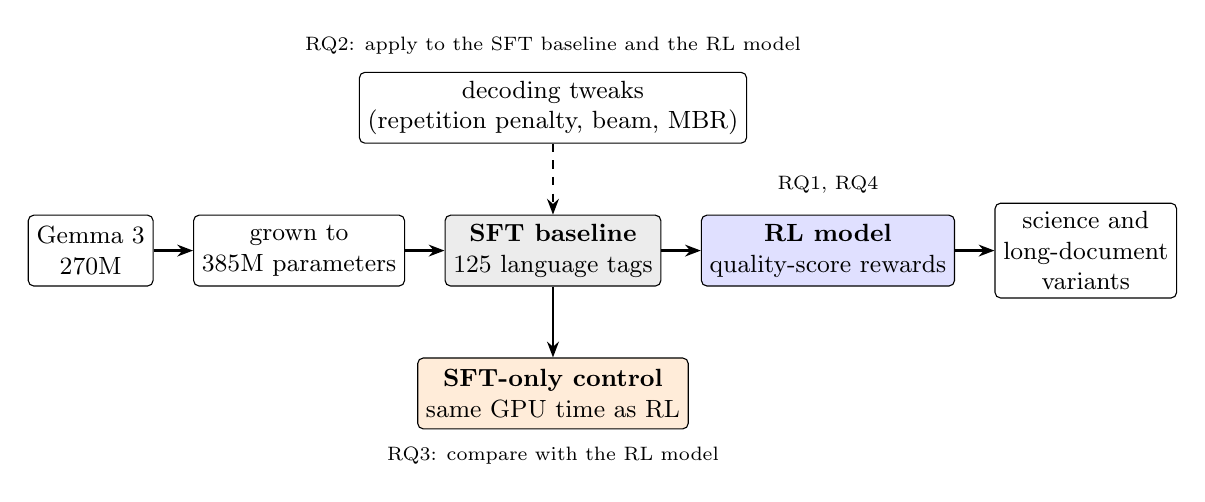
\begin{tikzpicture}[font=\small, node distance=5mm, box/.style={draw, rounded corners=2pt, align=center, minimum height=9mm, inner sep=3pt}, arr/.style={-{Stealth[length=2mm]}, thick}, lab/.style={font=\scriptsize, align=center}]
\node[box] (g) {Gemma 3\\ 270M};
\node[box, right=of g] (grow) {grown to\\ 385M parameters};
\node[box, right=of grow, fill=gray!15] (sft) {\textbf{SFT baseline}\\ 125 language tags};
\node[box, right=of sft, fill=blue!12] (rl) {\textbf{RL model}\\ quality-score rewards};
\node[box, right=of rl] (sci) {science and\\ long-document\\ variants};
\node[box, below=9mm of sft, fill=orange!15] (ctl) {\textbf{SFT-only control}\\ same GPU time as RL};
\node[box, above=9mm of sft] (dec) {decoding tweaks\\ (repetition penalty, beam, MBR)};
\draw[arr] (g) -- (grow); \draw[arr] (grow) -- (sft); \draw[arr] (sft) -- (rl); \draw[arr] (rl) -- (sci);
\draw[arr] (sft) -- (ctl); \draw[arr, dashed] (dec) -- (sft);
\node[lab, below=1mm of ctl] {RQ3: compare with the RL model};
\node[lab, above=1mm of dec] {RQ2: apply to the SFT baseline and the RL model};
\node[lab, above=1.5mm of rl] {RQ1, RQ4};
\end{tikzpicture}
\caption{Overview. A 270M model is grown to 385M parameters and fine-tuned (the SFT baseline), then trained with reinforcement learning (the RL model). Two controls ask what else could give the same gain: decoding changes (RQ2) and more fine-tuning for the same GPU time (RQ3).}\label{fig:overview}
\end{figure*}

\textbf{Model.} We start from Gemma-3-270m-it \citep{gemmateam2025gemma3} and add layers to reach 385M parameters (39 layers) \citep[cf.][]{wu2024llamapro,kim2023solar}. The task is English to one of 125 languages. A single extra token in the vocabulary names the target language, and the model answers with that token followed by the translation.

\textbf{Step 1: supervised fine-tuning (the SFT baseline).} We train on English-to-African sentence pairs and instruction data. Before training, we remove every pair that matches the text of any benchmark we later use, checked on both sides of the pair. Part of the data comes from NLLB-mined sentences and a collection of translated instructions; we report their share and licences in the Ethical considerations. Training uses the Muon optimiser \citep{liu2025muon} and takes about 45 hours on one A100 GPU (Appendix~\ref{app:hyper}).

\textbf{Step 2: reinforcement learning (the RL model).} We use GRPO \citep{shao2024deepseekmath}. For each English text the model samples 16 translations. Each translation receives a reward, and the model is nudged towards translations that score above the average of their group and away from those below it; a penalty keeps the model close to its starting point. Three stages follow one another, and the first does most of the work (Section~\ref{sec:rq4}). The reward has three parts. (i) A translation that fails a hard check scores the minimum: wrong or missing language tag, no end of text, a copy of the input, repetition, the wrong language, or an implausible length. (ii) Otherwise a quality score without a reference translation rates the output. We combine two quality models \citep{wang2024africomet,li2025ssacomet}, taking their mean unless they disagree strongly, and for languages without a validated quality model we reward agreement with the group's other samples. (iii) Small penalties discourage, among other things, unusual length, missing numbers or names, and missing diacritics. Exact settings are in Appendix~\ref{app:hyper}.

\textbf{Variants.} The \emph{SFT-only control} continues SFT from the baseline for the same GPU time as the RL stages, using half replay data and half extra English-to-X pairs for 19 languages \citep{gritta2026translatepsy}. The \emph{science variant} adds a short fine-tuning step on science text from AfriScience-MT \citep{abdulmumin2026afriscience} and then a second RL run; the \emph{long-document variant} adds RL on long inputs. Internal names used in the appendix tables are listed in Appendix~\ref{app:glossary}.

\section{Experimental Setup}\label{sec:eval}
% [M11 CT1-CT6 X1 X2 X5 X7 X9]
\textbf{Benchmarks.} We translate English into African languages on the standard FLORES+ devtest set \citep{oldi2025floresplus} (1,012 sentences; 54 languages), NTREX-128 \citep{federmann2022ntrex} (24 languages) and MAFAND-MT \citep{adelani2022mafand} (15 languages). Smaller sets, SmolSent \citep{caswell2025smol}, SALT \citep{akera2022salt}, GlotStoryBook \citep{kargaran2023glotlid}, IbomMT \citep{kalejaiye2025ibom} and FLORES-MOZ \citep{moznlp2026floresmoz}, appear in the appendix, as does AfriScience-MT \citep{abdulmumin2026afriscience} for science text. Unless stated, we report the average over languages, with each language counting equally.

\textbf{Metrics.} \emph{chrF++} compares character and word n-grams of the output with a human reference; higher is better. \emph{Held-out AfriCOMET} is a learned score that compares source, output and reference; we never use it as a reward. The \emph{finished rate} is the share of outputs that end properly; the \emph{loop rate} is the share that repeat themselves. Both are the checks our reward also uses, so they are not independent evidence of better translation. We computed chrF++ with sacreBLEU 2.6.0 (word order 2, otherwise defaults) after Unicode normalisation; the full signature string was not saved.

\textbf{Avoiding self-deception.} First, \emph{independence}: the metrics inside the reward (the two quality models, agreement between samples, and the finished, repetition and language checks) are not evidence that RL helped. Our evidence is chrF++ and held-out AfriCOMET against human references (Appendix~\ref{app:indep}). Second, \emph{paired tests}: every difference is a paired bootstrap over test sentences with a 95\% interval, which covers sentence variance but not training randomness. Third, \emph{contamination}: besides filtering the training pairs, we scanned 26 million training samples against all benchmark text and found no benchmark sentence of three or more words (Ethical considerations list the residuals). Fourth, \emph{seeds}: every model is one training run; we measured seed noise only for the first RL stage on 20 languages.

\textbf{Decoding.} All main results use greedy decoding with up to 768 new tokens (vLLM, bf16). The \emph{repetition penalty} used as a control is a decoding setting that discourages repeated tokens; we chose its strength on a development set by a rule fixed in advance. Beam search and MBR decoding are described where they appear.

\section{Results}\label{sec:results}

\subsection{RL against SFT, and what a decode-time guard recovers}\label{sec:rlsft}
% [R1 R2 R3 R4 R5 R6 R13 D5; EVID tables 1-2; E01] GATE E-01
``SFT'' is the 385M SFT final; ``RL'' is the final general RL model (mixed-stage best); 214 rows flagged by the contamination audit are removed. RL improves \chrfpp{} on every benchmark (Table~\ref{tab:headline}); plain chrF over the 93 cells improves by $+8.59$ \ci{+8.43}{+8.76} and held-out AfriCOMET (76 cells) by $+0.0631$ \ci{+0.0620}{+0.0643}. All 54 FLORES+ and 24 NTREX languages improve on \chrfpp{}, chrF and AfriCOMET with intervals above zero; on MAFAND-MT 14 of 15 improve (pcm $-0.25$ \ci{-0.69}{+0.30}).

\begin{table}[t]
\centering\footnotesize\setlength{\tabcolsep}{2pt}
\caption{RL against SFT (language-macro \chrfpp{}, clean rows, 95\% paired bootstrap, one seed).}\label{tab:headline}
\begin{tabular}{@{}lrrl@{}}
\toprule
benchmark (n) & SFT & RL & RL $-$ SFT\\
\midrule
FLORES+ (54) & 22.85 & 31.66 & $+8.81$ \ci{+8.59}{+9.03}\\
NTREX (24) & 29.25 & 37.17 & $+7.91$ \ci{+7.69}{+8.12}\\
MAFAND-MT (15) & 35.77 & 40.78 & $+5.01$ \ci{+4.76}{+5.23}\\
all 93 cells & 26.59 & 34.55 & $+7.96$ \ci{+7.82}{+8.12}\\
\bottomrule
\end{tabular}
\end{table}

\textbf{Finishing and looping.} On FLORES+ (finished / loop / hypothesis-to-reference length) the SFT has 0.829 / 0.209 / 3.03, RL stage A 0.983 / 0.068 / 1.33 and the mixed best 0.995 / 0.048 / 1.14 (Appendix~\ref{app:rlsft}). Cutting the SFT's looping outputs at the loop onset, without changing the translation, lifts the SFT from 26.59 to 30.49 \chrfpp{}: \textbf{49\% of the gain is recovered by cutting loops}. 67 to 70\% of the gain sits in rows where either model failed, and about 41\% of the AfriCOMET gain is finishing. On rows where the SFT finished and did not loop, RL is still $+2.41$ \ci{+2.33}{+2.49} \chrfpp{} and $+0.0366$ AfriCOMET ahead, significant in 50 of 54 FLORES+ languages; the estimates favour different models and agree in sign and rough size.

\textbf{Decode-time loop guard (E-01).} Greedy decoding with a vLLM frequency penalty of 0.10 (best of a seven-setting dev grid; plain greedy 34.50, best 37.36 dev \chrfpp{}) gives SFT $26.59\to30.48$ and RL $34.55\to34.84$ \chrfpp{} over the 93 cells, and AfriCOMET (76 cells) SFT $0.565\to0.583$, RL $0.628\to0.631$ (Figure~\ref{fig:decomp}). \textbf{A guard on the SFT recovers the same 49\% of the \chrfpp{} gain (29\% of the AfriCOMET gain) without RL}; RL with the guard minus SFT with the guard is $+4.37$ \ci{+4.28}{+4.46} \chrfpp{} and $+0.0479$ \ci{+0.0469}{+0.0490} AfriCOMET ($+2.63$ \ci{+2.56}{+2.70} \chrfpp{} on rows where the guarded SFT is clean). Caveats: the optimum (0.10) lies at the edge of the grid, so the control may be under-tuned; a post-hoc dev-only extension was still rising (SFT dev \chrfpp{} 37.36 at 0.10, 37.97 at 0.20, 38.00 at 0.30, 38.25 at 0.50) and no full evaluation with a stronger penalty was run; one seed. With the guard, FLORES+ zgh and MAFAND-MT pcm are significantly worse for RL than for the SFT.

\begin{figure*}[t]
\centering
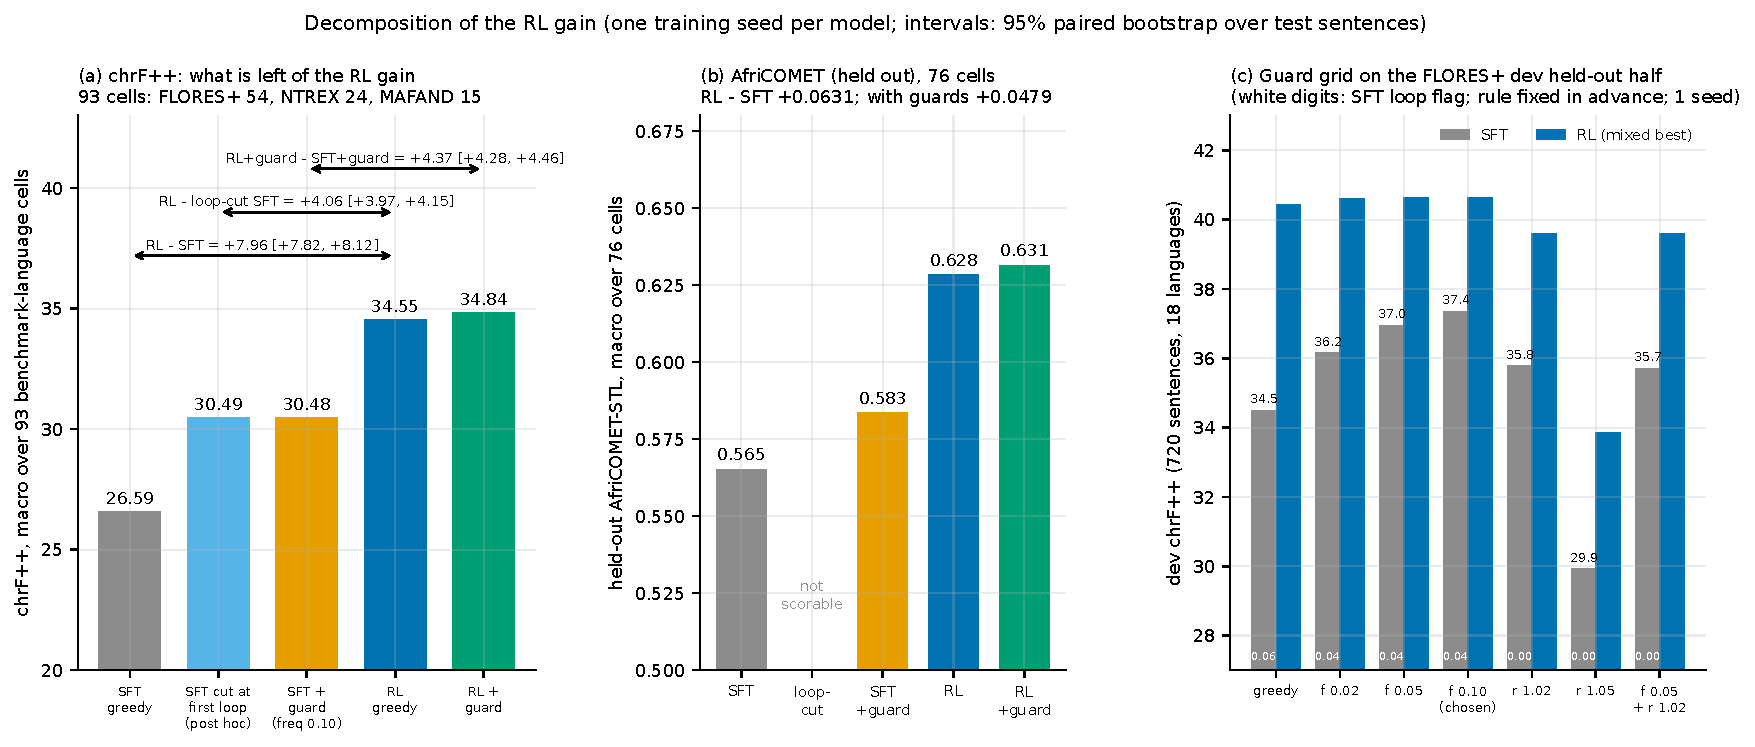
\includegraphics[width=\textwidth]{figures/fig3_decomposition_guard.pdf}
\caption{Decomposition of the RL gain with the decode-time guard (E-01). (a) Language-macro \chrfpp{} over 93 cells: SFT 26.59, SFT cut at its first loop 30.49 (post hoc), SFT with frequency penalty 0.10 30.48, RL 34.55, RL with guard 34.84; arrows give paired differences with 95\% CI. (b) Held-out AfriCOMET over 76 cells. (c) The seven-setting guard grid on the FLORES+ dev held-out half (720 sentences, 18 languages); the optimum (0.10) lies at the edge of the grid. One seed per model.}\label{fig:decomp}
\end{figure*}

\textbf{Growth and the earlier model.} The 385M SFT is significantly better than A0 on seven of eight benchmarks (FLORES+ $+5.31$ \ci{+5.13}{+5.50}, 46 languages; the comparison confounds depth with the extra stage-B SFT). In the same harness, on rows clean for both generations (E-13), it is behind our earlier 270M SFT on FLORES+ ($-2.35$ \ci{-3.25}{-1.38}), NTREX ($-4.13$) and MAFAND-MT ($-3.54$); after RL it is level on FLORES+ ($+0.35$ \ci{+0.08}{+0.62}) and NTREX ($+0.02$ \ci{-0.07}{+0.11}) and $1.55$ \chrfpp{} lower on MAFAND-MT, with data, steps, tokenizer layout and reward differing and only 4.7\% of FLORES+ rows kept (Appendix~\ref{app:sft}).

\subsection{Independent audit of the loop flag}\label{sec:degen}
% [R19-R24 DEGEN]
The reward's loop flag is the guard the RL was optimised against, so a missed loop type would be undercounted for RL. We re-measured with a detector sharing the idea but none of the code or constants (lzma-compressed size relative to human references of the same benchmark, language and length; repeated character 8-grams; repeated word 3-grams; each threshold set so that 0.1\% of 122,585 human references fire it). \textbf{The reward's flag is a lower bound:} on mixed-best FLORES+ the independent detector flags 1.77 \ci{1.71}{1.84} times as many outputs (0.0851 against 0.0480; SFT 0.3107 against 0.2095, ratio 1.48). The extra rows are finished partial repetitions: if they scored the average of their language's unflagged rows, mixed-best macro \chrfpp{} would rise by at most 0.19 (FLORES+), against 0.46 for the SFT, so the decomposition changes by 3.0\% to 4.4\% of the RL gains at most. Two further findings: 24.5\% of the 2,079 mixed-best rows above twice the reference length are flagged by neither detector, and \textbf{English output rises in the Arabic dialects and Tamazight} (aeb 0.215 to 0.449, ary 0.041 to 0.394, arz 0.006 to 0.098, zgh 0.001 to 0.049, SFT to mixed best; languages outside the RL prompt pool), so part of ``RL loops less'' there is a change from loops to English, while their \chrfpp{} stays at 2 to 9 (Appendix~\ref{app:degenapp}).

\begin{figure*}[t]
\centering
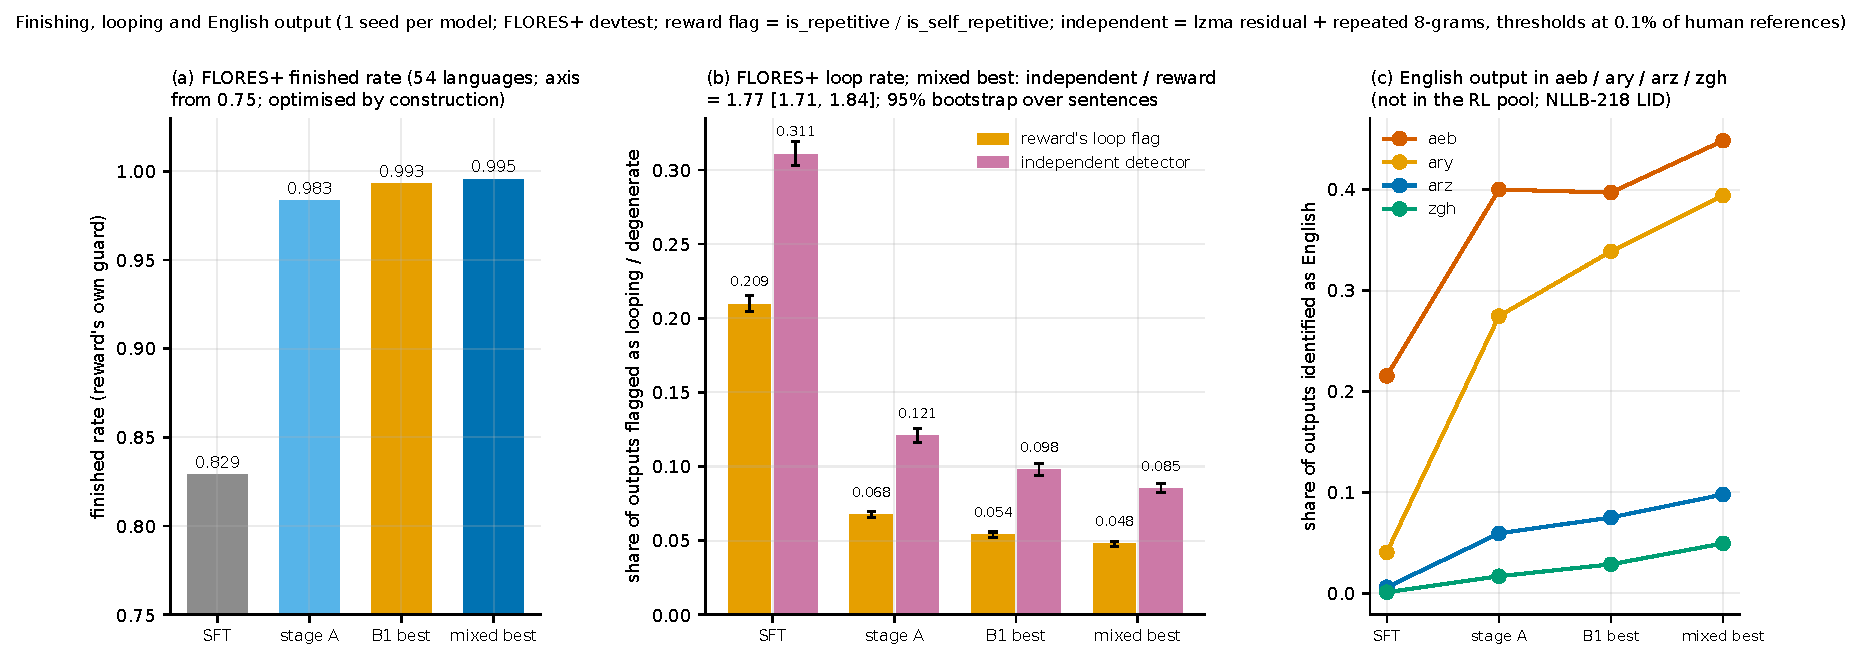
\includegraphics[width=\textwidth]{figures/fig7_loops_finishing.pdf}
\caption{Finishing, looping and English output on FLORES+ devtest (language macro, one seed per model). (a) Finished rate (54 languages; axis from 0.75). (b) Reward loop flag against the independent detector; error bars 95\% bootstrap over source sentences. (c) Share of outputs identified as English (NLLB-218 LID, $p\ge0.5$) in four languages outside the RL prompt pool.}\label{fig:loops}
\end{figure*}

\subsection{Where the gain accrues; seeds and ablations}\label{sec:seeds}
% [R8 E04 E11 M10 R17 R18]
Stage A gives 94\% of the SFT-to-B1 gain on FLORES+ (7.96 of 8.50); B1 adds $+0.54$ \ci{+0.49}{+0.59} and the mixed stage $+0.31$ \ci{+0.26}{+0.35} (NTREX $+0.30$, $+0.18$; MAFAND-MT nothing). B1 final (step 135) equals B1 best within noise. \textbf{Seeds (E-04).} Two extra runs of the stage-A recipe (100 steps, 20 languages, 49 cells) gain $+5.96$ \ci{+5.80}{+6.11} and $+5.90$ \ci{+5.74}{+6.05} \chrfpp{} over the SFT; they differ by \textbf{0.06} \ci{-0.02}{+0.14}. On those languages B1 best is $+0.17$ \ci{+0.12}{+0.21} over stage A, about three times the seed difference, while the mixed step is $+0.07$ \ci{+0.02}{+0.11}, the size of the seed difference: \textbf{we do not call the mixed step a gain}. This is one pair of seeds at step 100, not a seed study of later stages. RL aimed at eight weak West-African languages (85 steps, MBR guide) adds $+0.03$ \ci{-0.06}{+0.12} on its targets against a pre-registered $+1.0$ (negative result).

\textbf{Ablations (E-11).} One run per arm, 100 steps, forks of seed 2's step-40 state (Figure~\ref{fig:seeds}). Removing all four stage-A features costs \textbf{0.32} \ci{0.23}{0.41} \chrfpp{} (about 5\% of the gain, five times the seed difference); removing the reference domain costs 0.16 \ci{0.08}{0.25}; removing the beam guide costs 0.09 against seed 2 but $0.04$ \ci{-0.04}{+0.11} against seed 3, \textbf{not separable from seed noise}, for 25\% more step time. The KL rise is not caused by the features (median KL of steps 81 to 90: 0.116 without any feature, 0.120 to 0.123 in the other arms). The features are design choices with a small measured benefit.

\begin{figure*}[t]
\centering
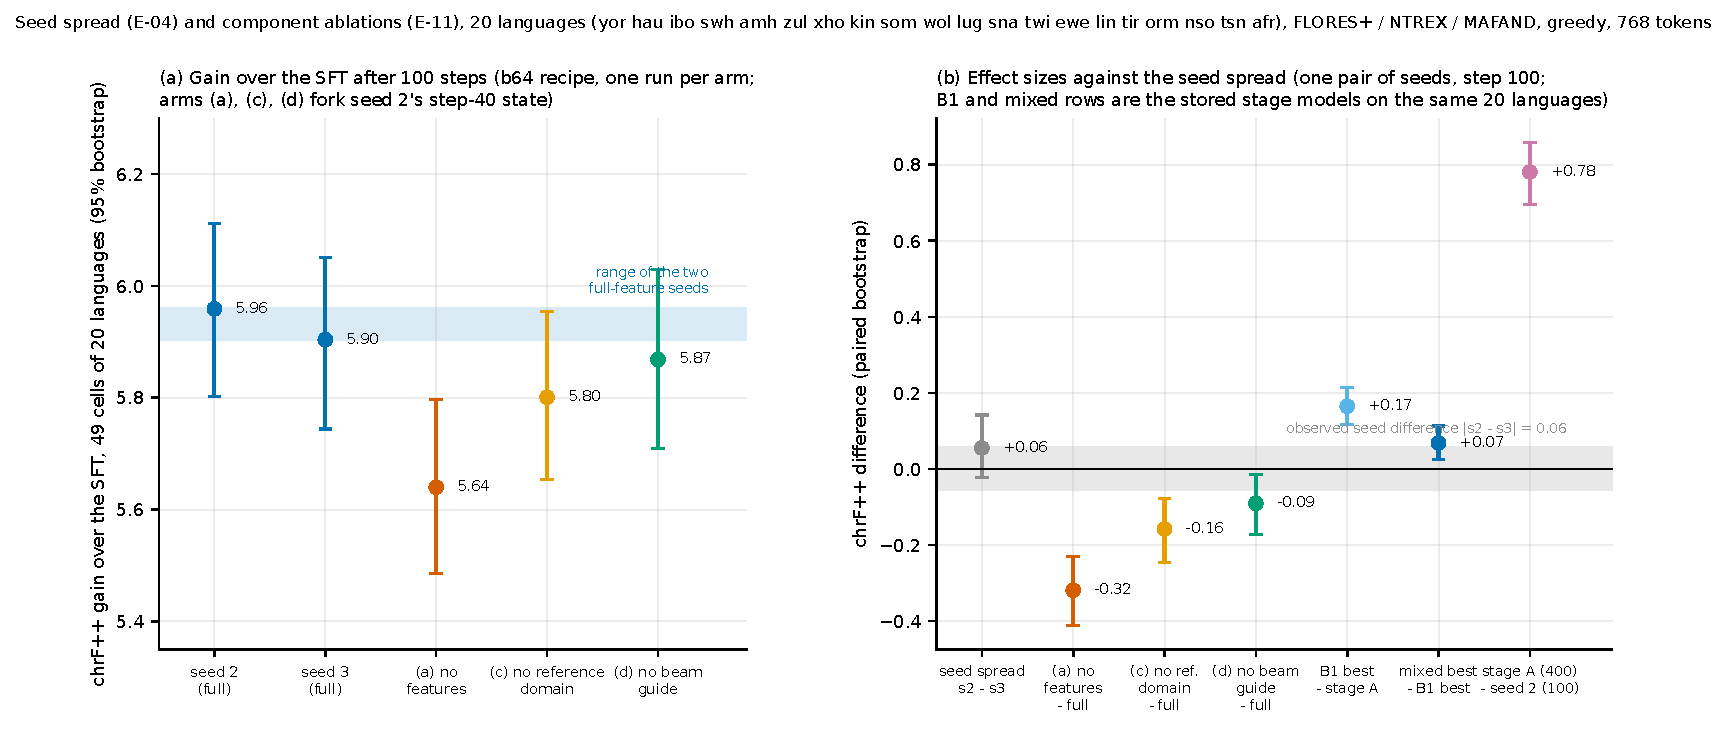
\includegraphics[width=\textwidth]{figures/fig16_e04_e11_seeds_ablations.pdf}
\caption{Seed spread (E-04) and ablation arms (E-11), 20 languages, 49 cells, greedy, 768 tokens, 95\% paired bootstrap. (a) \chrfpp{} gain over the SFT after 100 steps for two full-feature seeds and three ablation arms (shaded: range of the two seeds). (b) Effect sizes against the observed seed difference $|s_2-s_3|=0.06$: ablation arms minus seed 2, the B1 and mixed steps on the same languages, and the 400-step stage A minus seed 2. One pair of seeds, step 100.}\label{fig:seeds}
\end{figure*}

\subsection{Beam search and MBR (E-02)}\label{sec:decoding}
% [D1-D7 E02]
On 4,000 sentences (20 languages $\times$ 200 FLORES+ sentences) at 768 tokens, vLLM's beam search lets a runaway continuation beat every ended hypothesis, so the primary beam-4 (amended before any score) stops when 4 hypotheses have ended; a Hugging Face-style rule (\texttt{early\_stopping=False}) is a second beam. MBR-16 uses 16 samples plus the greedy output with \chrfpp{} as utility (metric-matched). Decoders help the SFT (beam-4 $+3.71$ \ci{+2.78}{+4.47}, MBR-16 $+5.96$ \ci{+5.37}{+6.49} \chrfpp{}); for the RL model MBR-16 adds $+0.92$ \ci{+0.81}{+1.03}, beam-4 (stop at 4) $-0.77$ \ci{-1.45}{-0.25} and the HF-rule beam $+0.83$ \ci{+0.67}{+1.00}: the sign of the RL beam result depends on the stopping rule. \textbf{Decoding does not replace RL}: RL greedy is $+1.60$ \ci{+1.34}{+1.88} \chrfpp{} ahead of the best decoded SFT (MBR-16, about 17 times the compute). RL minus SFT shrinks from $+7.56$ (greedy) to $+3.07$ (beam-4) and $+2.52$ (MBR-16): the RL gain is partly the same repair. Caveats: 20 languages, one checkpoint each; the beam numbers of an earlier 256-token study are not comparable (Appendix~\ref{app:decoding}). \textbf{Precision (E-09b):} bf16 and fp32 outputs differ between engines, but the SFT in fp32 on the full set scores $-0.04$ \ci{-0.13}{+0.07} \chrfpp{} against bf16 over the 93 cells, and the RL gain on FLORES+ is $+8.97$ \ci{+8.71}{+9.20} over the fp32 SFT against $+8.81$ over the bf16 SFT, so the bf16 harness does not overstate it; the RL model was not run in fp32.

\begin{table*}[t]
\centering\small\setlength{\tabcolsep}{3pt}
\caption{\chrfpp{} at 768 new tokens, language macro over 20 languages, 4,000 sentences per row, 95\% paired bootstrap (E-02).}\label{tab:e02}
\begin{tabular}{@{}lll@{}}
\toprule
decoding & SFT & RL (mixed best)\\
\midrule
greedy & 32.31 \ci{31.43}{33.38} & 39.87 \ci{39.17}{40.62}\\
beam-4, stop at 4 ended & 36.02 \ci{35.13}{36.95} & 39.10 \ci{38.20}{39.96}\\
beam-4, HF rule & 33.26 \ci{32.22}{34.46} & 40.70 \ci{40.00}{41.42}\\
MBR-16 & 38.27 \ci{37.60}{39.01} & 40.79 \ci{40.09}{41.54}\\
\bottomrule
\end{tabular}
\end{table*}

\subsection{Matched-compute continued-SFT control (E-03)}\label{sec:control}
% [R14 CTL7-CTL11] reports/e03_sft_control_2026-11-05.md; GATE E-03
To ask whether the GPU time of the RL chain (8.66 \GPUh{}) would do as well as more SFT, we continued the SFT final for 6,000 steps (8.4 h) at a constant learning rate of $10^{-5}$ (chosen by a probe fixed in advance), with 16 replay packs and 16 packs of TranslatePsy English-to-X pairs \citep{gritta2026translatepsy} per step: NLLB-3.3B translations of MADLAD-400 sentences for 19 languages, 277,900 pairs each, scanned against the protected index and used once. The decision rule, primary endpoint (language-macro \chrfpp{} over 93 cells, RL minus control) and language panels were written down before any benchmark of the control was looked at. \textbf{Only the 6,000-step checkpoint was evaluated}; the stage-A-matched (3,100) and mixed-best-matched (4,800) checkpoints exist but were not evaluated.

\begin{table}[t]
\centering\footnotesize\setlength{\tabcolsep}{3pt}
\caption{Continued-SFT control against the RL mixed best; language-macro \chrfpp{}, clean rows, 95\% paired bootstrap; TP = the 19 TranslatePsy languages. Held-out AfriCOMET, RL $-$ control: $+0.0183$ (all), $-0.0249$ (TP), $+0.0883$ (other).}\label{tab:e03}
\begin{tabular}{@{}lccl@{}}
\toprule
cells & control & RL & RL $-$ control\\
\midrule
all (93) & 29.97 & 34.55 & $+4.58$ \ci{+4.45}{+4.70}\\
TP (47) & 41.37 & 41.34 & $-0.03$ \ci{-0.13}{+0.09}\\
other (46) & 18.32 & 27.61 & $+9.29$ \ci{+9.09}{+9.49}\\
\bottomrule
\end{tabular}
\end{table}

The registered rule had four conditions: lower bound of the overall difference above $+1.0$ (met: $+4.58$ \ci{+4.45}{+4.70}), AfriCOMET lower bound above 0 (met: $+0.0183$ \ci{+0.0172}{+0.0192}), difference above 0 on the other languages (met) and difference above 0 on the 19 TranslatePsy languages (\textbf{not met}: $-0.03$). \textbf{By the rule as registered the verdict is ``inconclusive''}, and we did not change the rule. Reading the panels: where a teacher-translated corpus exists, continued SFT matches RL in \chrfpp{}, largely fixes finishing and looping (FLORES+ finished 0.993 against 1.000 for RL), and is ahead on the neural metrics; on the other languages it changes almost nothing ($+0.15$ \chrfpp{} over the SFT on FLORES+, \ci{-0.03}{+0.32}), while RL improves them all from its own samples ($+9.29$). The overall endpoint alone reads ``RL is better'', the 19 languages alone ``comparable''; neither is the registered verdict. Caveats: one seed, one learning rate, one budget point; the control is not information-matched (NLLB-3.3B scores 38.80 against 26.30 for the SFT on 43 languages), and the TranslatePsy rows were filtered with AfriCOMET, SSA-COMET and MetricX, so those neural metrics favour the control; chrF and \chrfpp{} are the evidence.

\begin{figure*}[t]
\centering
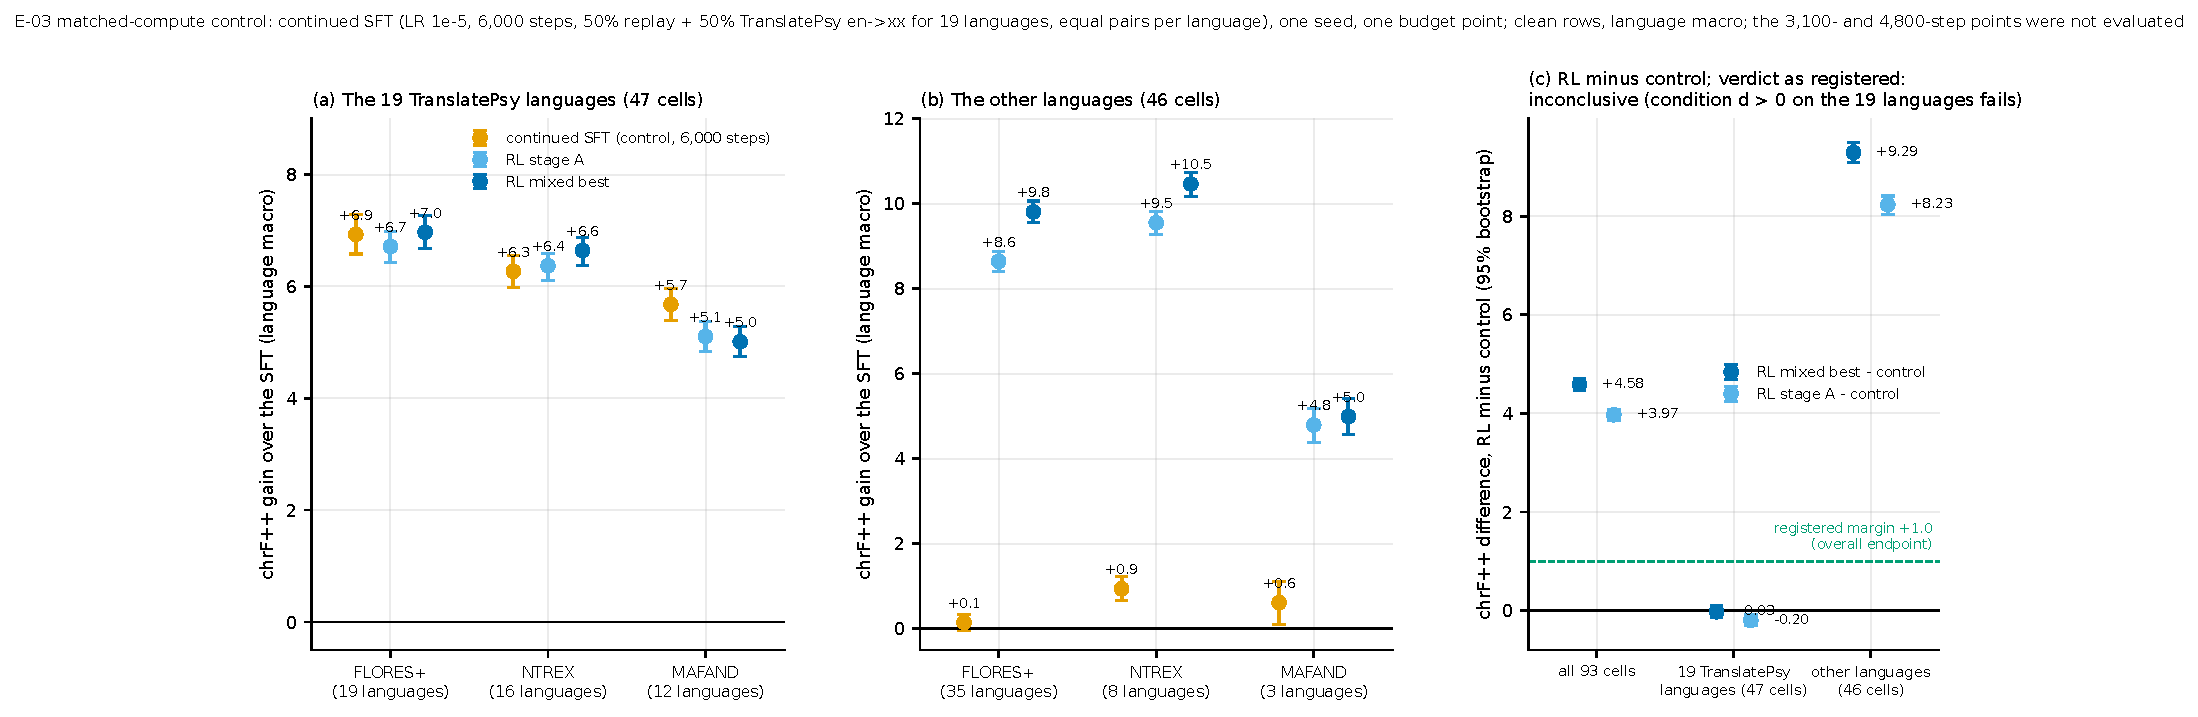
\includegraphics[width=\textwidth]{figures/fig14_e03_control.pdf}
\caption{Matched-compute continued-SFT control (E-03). (a, b) \chrfpp{} gain over the SFT (language macro, 95\% bootstrap) of the control, RL stage A and RL mixed best by benchmark, for the 47 cells of the 19 TranslatePsy languages (a) and the 46 other cells (b). (c) RL minus control for all 93 cells and for the two panels, with the registered $+1.0$ margin; the registered verdict is inconclusive. One seed per model; only the 6,000-step checkpoint was evaluated.}\label{fig:e03}
\end{figure*}

\subsection{Comparison with NLLB-200}\label{sec:nllb}
% [N1-N6 NLLBRL]
NLLB-200 3.3B (the 3.3B variant of its model card) has about 8.6 times the parameters of our 385M model. On the 43 languages shared with the published FLORES-200 devtest table, the mixed best reaches 35.54 \chrfpp{} against 38.80 for NLLB-3.3B ($-3.26$, language-bootstrap \ci{-4.29}{-2.20}; 92\%; SFT 26.30, $-12.50$, 68\%): RL closes 74\% of the gap, and the remaining gap is not a finishing artefact (the mixed best finishes at least 0.99 in every language). It matches or beats NLLB-3.3B on 7 of 43 languages, all in the lowest tertile (e.g. yor $+5.43$, fon $+2.95$); the largest gaps are amh $-11.28$, kin $-9.74$, kea $-8.72$. Caveats: FLORES-200 against FLORES+ references, NLLB beam against our greedy (beam and MBR move our \chrfpp{} by $-0.77$ to $+0.92$), the 11 hardest languages have no NLLB row, five of the 43 languages had an NLLB pseudo-reference reward term, the yor value is anomalously low, intervals are over languages, one seed. We state only that, size-aware, the model reaches 92\% of NLLB-3.3B's \chrfpp{} on these languages and matches or beats it on 7 of 43; we do not claim to beat NLLB or to be competitive with it overall.

\begin{figure*}[t]
\centering
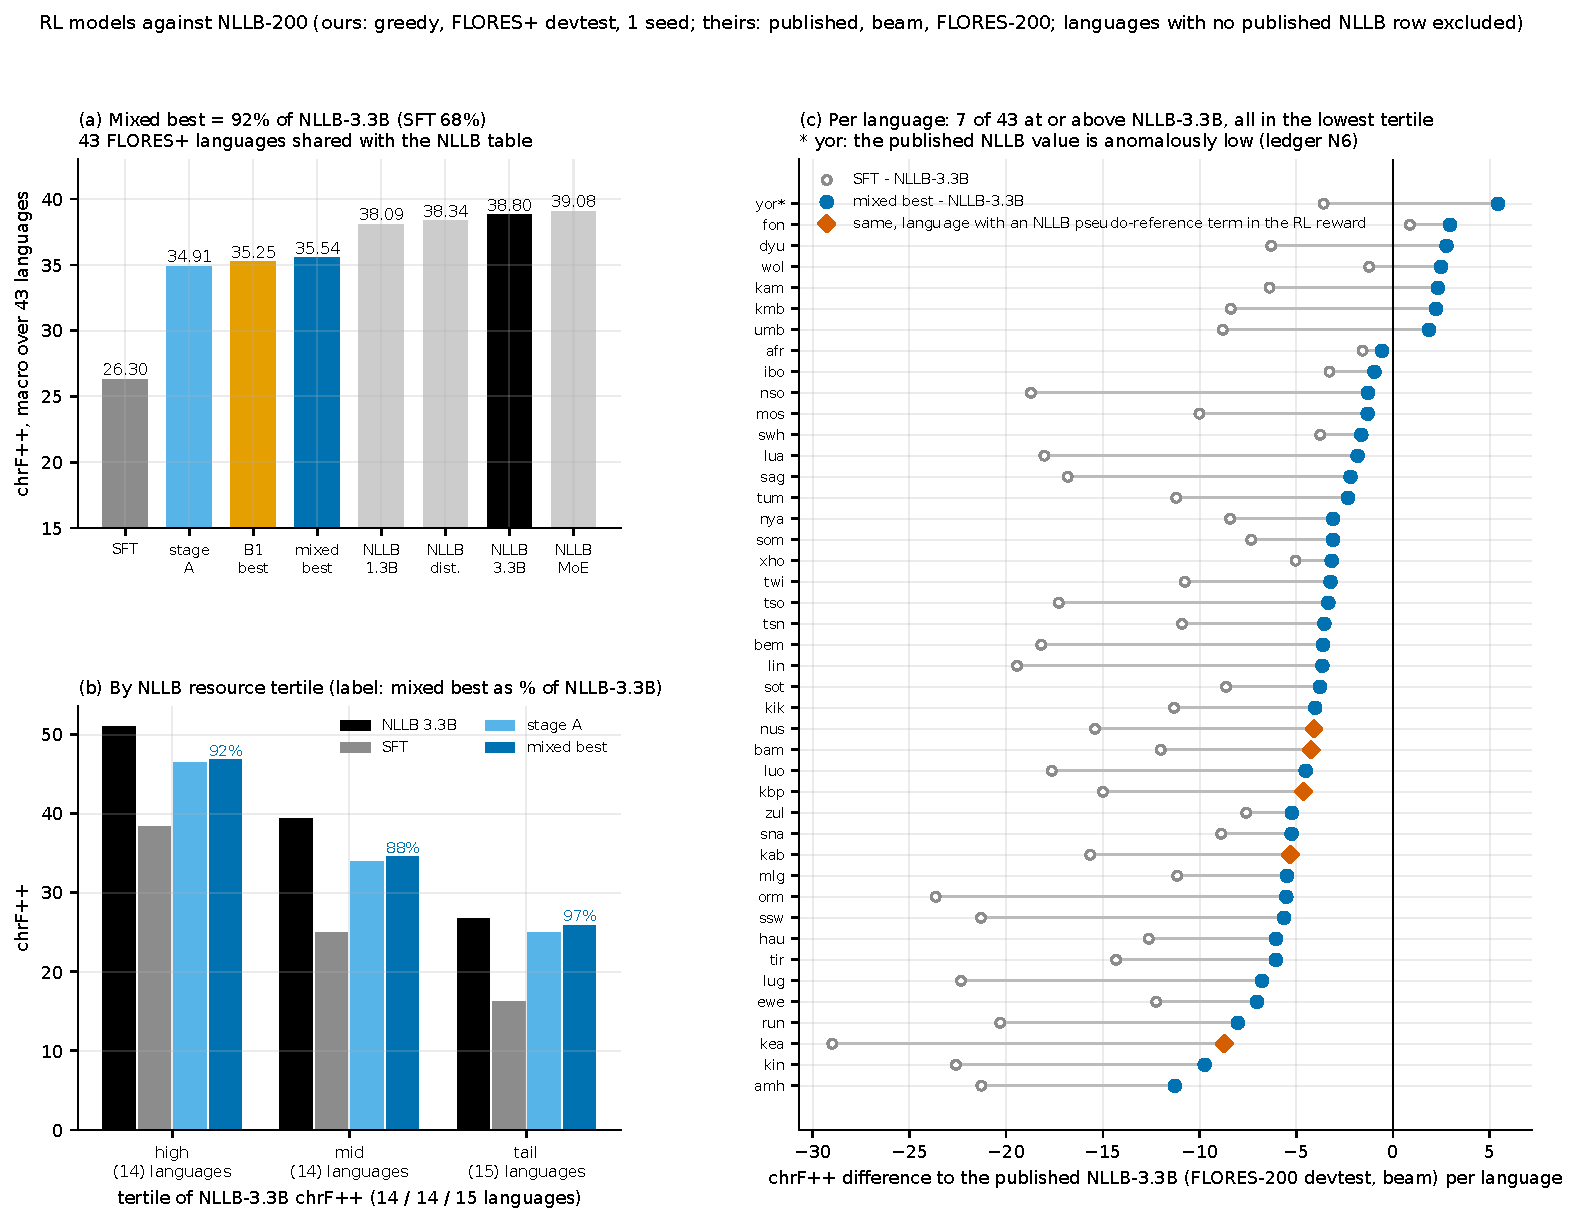
\includegraphics[width=0.62\textwidth]{figures/fig4_nllb_43.pdf}
\caption{RL models against NLLB-200 on the 43 shared FLORES+ languages (ours: greedy, one seed per model; NLLB: published FLORES-200 devtest, beam). (a) Language-macro \chrfpp{}: mixed best 35.54 against NLLB-3.3B 38.80 (92\%; SFT 68\%). (b) By tertile of NLLB-3.3B \chrfpp{} (14/14/15 languages). (c) Per-language difference to NLLB-3.3B, SFT (open) and mixed best (filled); orange diamonds: languages with an NLLB-3.3B pseudo-reference reward term; yor$^*$: anomalously low published value. Intervals are over languages only.}\label{fig:nllb}
\end{figure*}

\subsection{Science and long-document RL}\label{sec:science}
% [SC1-SC6 DL1-DL5 P4 E05 E15 E16]
A science SFT with weight interpolation ($\alpha=0.5$) gives surface gains on AfriScience-MT (chrF $+1.2$) and no SSA-COMET-QE gain (0.6130 to 0.6118). A science RL adds $+0.46$ chrF \ci{+0.27}{+0.65} and $+0.0053$ AfriCOMET on test sentences over its start, and nothing at document level. \textbf{The science SFT, not the science RL, carries the science gain (E-14):} the same RL started from the mixed best, without the science SFT, ends $-1.44$ chrF \ci{-1.61}{-1.25} and $-0.0082$ AfriCOMET \ci{-0.0101}{-0.0065} below the executed science RL and adds only $+0.26$ chrF \ci{+0.12}{+0.39} over its start, so by the registered rule the science SFT is needed; SSA-COMET-QE rates it level ($-0.0006$ \ci{-0.0018}{+0.0007}), a reward-family effect rather than evidence of quality. One seed, one out-of-memory restart, final checkpoint only (Appendix~\ref{app:docs}). Whole-document generation (4,096 tokens) fails for the 385M models; a long-document RL raises whole-document finishing from 0.70 to 0.82 ($+0.125$ \ci{+0.046}{+0.204}) and lowers the loop rate from 0.85 to 0.73, but 72 to 73\% of documents still loop and chunked decoding is required; the earlier 270M model is as good or better at document level. Table~\ref{tab:sci} gives sentence-level scores for every stage (SSA-COMET-QE is of the reward family; the first RL stage adds $+0.043$ and later stages at most $+0.005$ more, while chrF and AfriCOMET keep rising slightly).

\begin{table}[t]
\centering\footnotesize\setlength{\tabcolsep}{3pt}
\caption{AfriScience-MT test, sentence level (970 sentences per language; macro over amh hau lug nso yor zul; greedy; one seed per stage). SSA-QE = SSA-COMET-QE, of the reward family for every RL row.}\label{tab:sci}
\begin{tabular}{@{}lccc@{}}
\toprule
stage & chrF & AfriCOMET & SSA-QE\\
\midrule
SFT & 36.00 & 0.6064 & 0.5686\\
RL stage A & 45.06 & 0.6822 & 0.6118\\
RL mixed best & 45.40 & 0.6828 & 0.6130\\
science RL w/o SFT (E-14) & 45.66 & 0.6850 & 0.6153\\
science SFT ($\alpha=0.5$) & 46.63 & 0.6879 & 0.6118\\
science RL final & 47.10 & 0.6932 & 0.6158\\
long-document RL final & 47.16 & 0.6936 & 0.6165\\
\bottomrule
\end{tabular}
\end{table}

\section{Discussion and Conclusion}\label{sec:discussion}
% [paper.md 12.1-12.3; GATE E-01 E-03]
Under automatic metrics, RL with reference-free QE rewards beats the SFT everywhere, but about half of the \chrfpp{} gain (49\%; 29\% of the AfriCOMET gain) is finishing and looping that a one-line decode-time guard also removes, and beam/MBR decoding repairs a further part. What RL adds beyond a guarded SFT is $+4.37$ \chrfpp{}; nearly all of it arrives in the first stage, and the mixed step is not separable from seed noise. Our reading, only partly tested, is that the SFT's main defect is unguarded greedy decoding and that the hard-failure floor and the QE reward teach the policy to avoid it within about a hundred steps. Against continued SFT for the same GPU time the registered verdict is ``inconclusive'': the control matches RL on the 19 languages it has teacher data for and does nothing for the other 46 cells, so what RL contributes, in our data, is breadth. We do not claim that the \chrfpp{} beyond finishing is quality a human would confirm, that any reward component other than the stage-A features helped, or that the model is usable for Arabic dialects, Tamazight, Dinka, Tamasheq or Kanuri. In science translation the science SFT, not the science RL, carries the gain (E-14: the same RL without it ends $-1.44$ chrF \ci{-1.61}{-1.25} lower). Next experiments: stronger guards in full evaluation, the unevaluated control checkpoints, later-stage seeds and human judgement of outputs.

\FloatBarrier\label{coreend}
\clearpage
\section*{Limitations}
% [paper.md section 13; full list in the appendix of the full version]
\textbf{Automatic scoring only.} The references of FLORES+, NTREX-128 and MAFAND-MT are human translations, but all scoring is automatic: no human judgement of system outputs was collected. The neural scores belong to one family, and AfriCOMET has a length and entity bias.
\textbf{One training run per model.} We measured seed noise only for the first RL stage, on 20 languages and 100 steps, with one pair of extra seeds. The last RL step and per-language differences below about half a point cannot be separated from seed noise. A second seed of the SFT baseline is impractical (about 45 GPU-hours).
\textbf{The matched-compute control is one run:} one seed, one learning rate, one data mix with NLLB-3.3B targets and one evaluated stopping point. The repetition-penalty control chose its best value at the edge of the range searched.
\textbf{Rewarded metrics are not evidence.} The finished, repetition and language checks, and the quality scores the RL optimises, are part of the reward. The independent repetition detector shares the idea of the reward's check and cannot see non-repetitive failures.
\textbf{Ablations are limited:} three arms, 100 steps, one run each, 20 languages; later RL stages and most reward ingredients were not ablated, and mid-run changes (Ethical considerations) mean the stages are not one clean design.
\textbf{Decoding and engine.} Headline numbers use one inference engine in bf16. The two engines differ in bf16 but agree in fp32; we did not run the RL model in fp32. Beam search and MBR cover 20 languages and one beam width.
\textbf{Coverage and comparisons.} Fifty-one of the 125 languages have no reference test and are unscored. The model fails on Arabic dialects, Tamazight, Dinka, Tamasheq and Kanuri, where RL increases English output. Comparisons with the earlier 270M model and with NLLB mix differences in data, steps, test sets and decoding: our decoding is greedy, NLLB's is beam search, and on NTREX and MAFAND-MT only language-level NLLB averages exist (no sentence pairing, no AfriCOMET). Document results rest on 28 papers per language, and whole-document translation remains unusable.
\textbf{Not run.} Human judgement of outputs; the NLLB-data ablation; scans of packed training shards for contamination; a 54-language decoding study; a science fine-tuning step at full strength followed by RL; a second seed of the science run; long-document RL from the no-science-step model.

\section*{Ethical considerations}
% [DISCLOSURES sections 1-6; L1-L5 CT1-CT13 CTL1-CTL6; CFU]
\textbf{Data and licences.} NLLB-mined bitext (OPUS-NLLB, 43 languages; Fulah) is 14.4\% of the 3.990\,B stage-B pack tokens (10.84\% of the 5.043\,B tokens drawn in the whole SFT); with NLLB-Seed and the aligned part of Aya (NLLB-3.3B outputs) 18.7\%; with machine-translated Tumbuka instruction sets (system not stated, possibly NLLB) 22.8\%. NLLB models and outputs carry CC-BY-NC terms, which limits the commercial use of NLLB-derived data and signals, and a licence statement must accompany any release of the weights. Sources with unspecified or unconfirmed licences (the \texttt{*\_mt560} OPUS sets, 69\% of the main pair output, mostly Jehovah's Witnesses and Bible text; \texttt{multi-open}; AfroLingu-MT; an Efik New Testament sheet) need a legal decision, and religious text dominates many low-resource languages. IbomMT (CC-BY-NC-4.0) is a disclosed non-commercial exception. NLLB-3.3B pseudo-references (CC-BY-NC) are a reward signal for five languages, reward only. RL prompts (FineWeb-Edu, Wikipedia, news including BBC News with no declared licence and BBC copyright) are input text only. Gemma terms apply to the derived weights and its pretraining exposure cannot be excluded. Reward and monitor models, as declared on the Hub (read 2026-11-05): \texttt{ssa-comet-mtl}, \texttt{ssa-comet-qe} and the two AfriCOMET checkpoints apache-2.0; GlotLID \texttt{license: other} with \texttt{license\_name: apache-2.0-plus-notices} (Apache License 2.0 plus notices).

\textbf{Release and licence.} \anonreal{Checkpoints are anonymised for review and released on acceptance; the control checkpoint of E-03 is not released.}{The final RL model (branch \texttt{main}, the mixed best) is at \url{https://huggingface.co/AletheiaAING/gemma-0.4B-translate-rl}, the SFT model at \url{https://huggingface.co/AletheiaAING/gemma-0.4B-translate-sft} and the seed, ablation and E-14 weights at \url{https://huggingface.co/AletheiaAING/gemma-0.4B-translate-rl-experiments}; the control checkpoint of E-03 is not released.} At the last check the Hub repositories declare no licence field and have no model card; the Gemma terms of use apply to the derived weights, and the NLLB-derived and non-commercial data above limit commercial use \ownerdecision{confirm release licence}. The state, prompts, eval and reports repositories were private at the last check \ownerdecision{which parts of the data are released}.

\textbf{TranslatePsy.} \texttt{qvac/\allowbreak TranslatePsy-\allowbreak AfriSLM-\allowbreak Synthetic-\allowbreak Mix} (CC-BY-NC-4.0; targets are NLLB-3.3B translations of MADLAD-400 sentences filtered by AfriCOMET, SSA-COMET and MetricX) was used for the matched-compute control only. No TranslatePsy row is in the SFT, any RL stage, the science or long-document stages or any released weight; the control checkpoint is a research artefact that is neither released nor used in production. A good control result partly means ``distilling NLLB''. The NLLB-218 language-ID model (CC-BY-NC) was used for measurement only.

\textbf{Decontamination residuals (this pipeline, the clean 385M rerun).} The audit of the 385M training text finds no benchmark sentence of three or more words; benchmark rows that match are one- or two-word strings, numerals and names (NTREX 120 of 47,928 rows, 0.25\%; MAFAND-MT 94 of 20,009, 0.47\%; SmolSent 45 of 38,833; GlotStoryBook 15 of 3,426). The FLORES+ dev train half (440 ids) is in training on purpose and the held-out half is protected. A lexical fuzzy scan (56,975,939 pair rows, 4,277,612 instruction rows) finds no benchmark string of 8 or more tokens as a contiguous run, but strings of 4 to 7 tokens occur inside longer text (English side: MAFAND-MT 134 of 17,428, GlotStoryBook 30 of 898, NTREX 18 of 1,973, SALT 12 of 498) and 263 (string, benchmark) cases of 8+ token strings overlap training text by character 5-grams (candidates, effect on scores not measured). Stage A drew 6 flagged prompts of 28,120 (0.021\%) from seven unfiltered prompt files; 305 of 34,007 AfriScience-MT train rows (0.9\%) have their African-language sentence in the A0 pair data (test papers untouched). Embedding or MT-round-trip paraphrase scans and packed-shard scans were not run. Statements about the earlier 270M pipeline, whose training text held the English side of 95\% of FLORES+ devtest, do not apply to this rerun; its numbers appear only on rows clean for both generations.

\textbf{Analysis decisions and process.} Checkpoints were selected on a 720-sentence FLORES+ dev subset; the weak-language choice used devtest-derived per-language tables; the decomposition and family analyses were run after the results were known; the science headline metric changed after the interpolation rule was written. The RL preflight and stage-A gates failed and were overridden by the authors; stage A was stopped at step 40 and resumed with four features; B1 was restarted twice and the mixed stage once (the hacking alarm was loosened); the science-RL step cap was extended from 150 to 190 and the run stopped on a dev plateau after 160 steps; the long-document RL lost about 4.5 of 7.7 h to a crash loop, and the E-14 run had one out-of-memory restart (steps 21 to 38 replayed; the later records are used). LibreTexts rows were removed from the long-document pool before it started.

\textbf{Intended use, risks and dual use.} Outputs are machine translations of unverified quality for languages without human judgement, with documented failure modes (Arabic dialects, Tamazight, Dinka, Tamasheq and Kanuri are not usable; RL increases English output there; use sentence by sentence, not on whole documents). The model should not replace NLLB-class systems or be used where mistranslation is costly (health, legal, safety). As with any translation model it can be used to produce text at scale in under-served languages, including spam or misleading content, and we release no content-filtering component. Released artefacts are anonymised for review and released on acceptance.

\ifanon\else
\section*{Author contributions}
\textit{[Placeholder, to be filled by the lead author: one sentence per person describing what that person contributed (for example design, data, training, evaluation, writing). Authorship is based on contribution.]}
\fi
\bibliography{refs}
\bibliographystyle{acl_natbib}

\clearpage
\appendix
\label{appstart}
\onecolumn
% Appendix: generated from paper_385m/paper.md by a small converter, then kept as hand-editable LaTeX. Report keys and claim IDs are in % comments.

\FloatBarrier

\section{Hyper-parameters, recipe and reward details}\label{app:hyper}

This appendix collects the SFT and RL settings that Sections~\ref{sec:method} and~\ref{sec:method} summarise.

\subsection{SFT recipe and learning-rate schedule}

\textbf{Recipe.} Samples are packed into 4,096-token packs (one language per pack, block-diagonal attention) at 32 packs = 131,072 tokens per step; each pack is used once. Optimiser: Muon (momentum 0.95, 5 Newton-Schulz steps) on the 2-D decoder matrices and AdamW (betas 0.9/0.95) on embeddings and norms, weight decay 0.01, gradient clipping 1.0, 3\% linear warm-up then cosine decay, seed 1234. The learning-rate schedule, read from the executed per-shard configs, is: SFT-1 (\texttt{g1a}, 1,500 steps) peak 5e-5, cosine to 50\% of the peak (2.5e-5); shard 1 (\texttt{g1b\_\allowbreak{}s1}) peak 5e-5, cosine to 80\% (4e-5); shards 2-5 (\texttt{g1b\_\allowbreak{}s2}..\texttt{g1b\_\allowbreak{}s5}) peak 3e-5 (lowered from 5e-5 on 2026-11-01 because of forgetting in tiny languages), cosine to 80\% (2.4e-5); shard 6 (\texttt{g1b\_\allowbreak{}s6}) peak 3e-5, cosine to 10\%, so the last step runs at 3.0e-6. Every shard starts a fresh Muon state with a 3\% linear warm-up. SFT-2 runs in six shards of about 4,800 to 5,300 steps, with tail-language replay from shard 2. Executed stage B: 31,353 steps, 4.109 B tokens, 5.14 s per step on an A100 (44.8 h); 32,853 steps in all with SFT-1. Final validation loss: macro 1.3412, micro 1.2846 over 78 languages (end of SFT-1: 1.7847). The macro rises from 1.78 to 1.98 at the end of shard 1 because new languages enter the validation set at stage 2.  
% src: VERIFIED against the executed per-shard configs (`learning_rate`, `min_lr_ratio`, `warmup_ratio`, `init_from` keys): `reports/data/e23_hygiene_2026-11-04/sft_configs/g1a.yaml`, `g1b_s1.yaml` ... `g1b_s6.yaml` (copies of the box files `clean_sft_small/run/configs/growth1/`). The repository templates `gemma_mt/configs/growth1/g1a.yaml` (5e-5, min_lr_ratio 0.5) and `g1b.yaml` (5e-5, min_lr_ratio 0.1) are NOT the executed shard configs: `g1b.yaml` is the single-shard template (peak 5e-5, floor 10%); `gemma_mt/configs/clean_rerun_sft/` holds the A0 configs only. Resolves the HYG M4 vs CTLP disagreement: HYG's "cosine to 10%" is right only for shard 6 (and the g1b template); CTLP's 0.8 for shards 2-5 is right; shard 1 also 0.8 and SFT-1 0.5, neither stated in HYG or CTLP. Other keys common to all: Muon momentum 0.95, 5 NS steps, weight decay 0.01. Validation: HYG M4 (sft_385m_curve.csv, sft_385m_val_by_language_final.csv); NLLBLINK for 44.8 h

\begin{figure}[t]
\centering
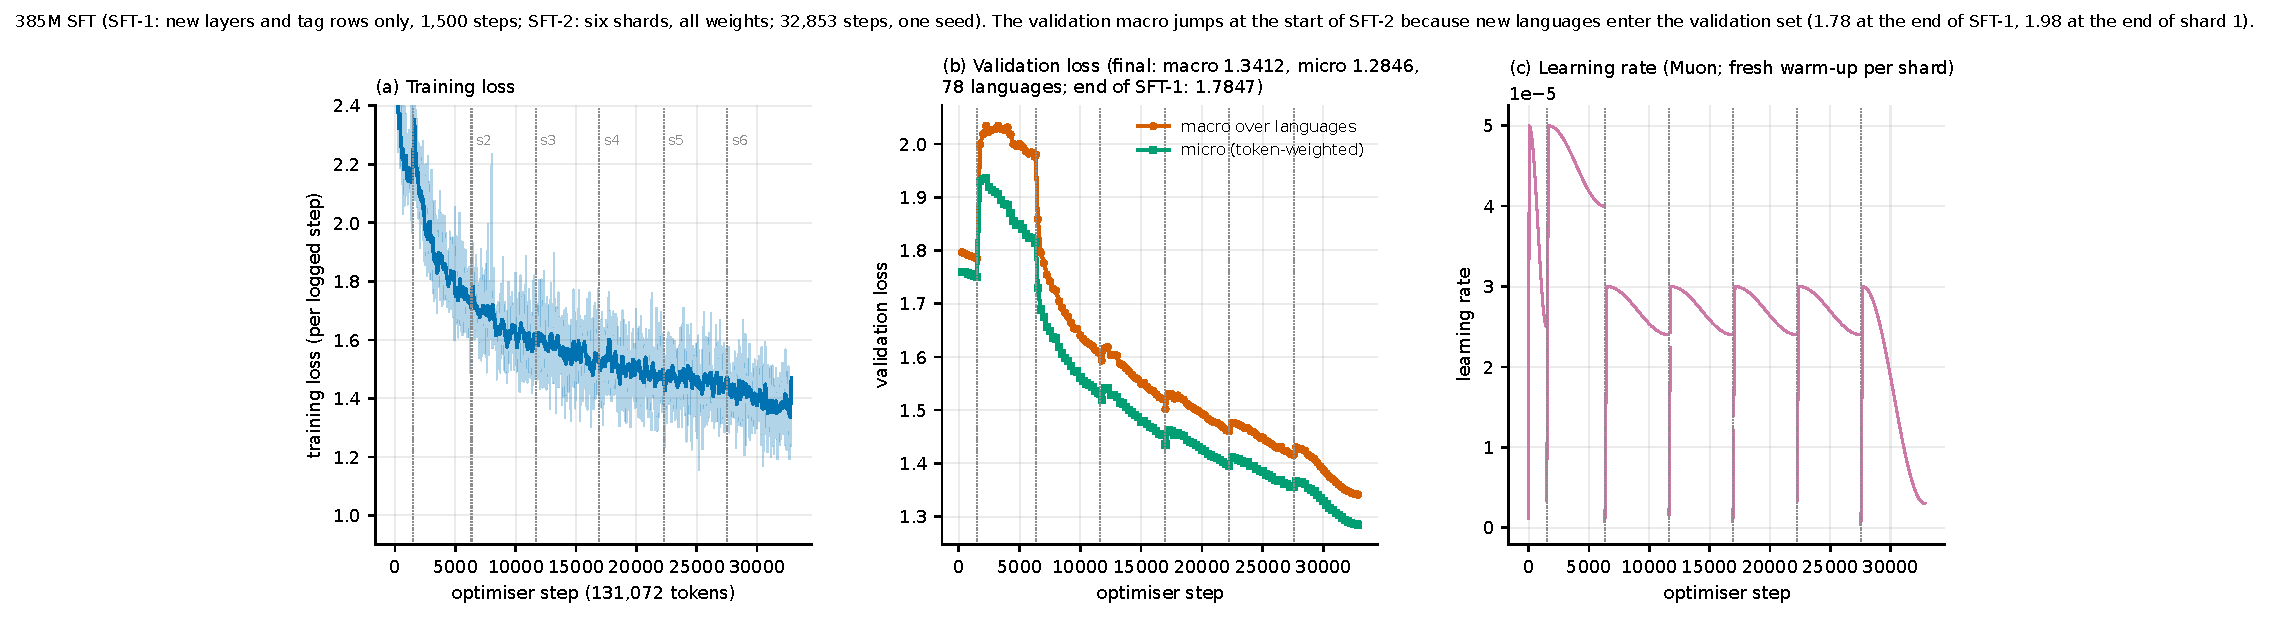
\includegraphics[width=1.00\linewidth]{figures/fig13_sft_validation_curve.pdf}
\caption{Training of the 385M SFT (one seed): (a) training loss per logged step (thin) and 20-point mean (thick), (b) validation loss (macro over languages and token-weighted micro) and (c) learning rate over the 32,853 optimiser steps of SFT-1 (1,500 steps, new layers and tag rows only) and the six SFT-2 shards (dotted lines); the validation macro jumps at the start of SFT-2 because new languages enter the validation set, and the learning-rate panel shows the per-shard schedule of Section~\ref{sec:method}. Final validation loss: macro 1.3412, micro 1.2846 over 78 languages. Source: \texttt{reports/\allowbreak{}data/\allowbreak{}e23\_\allowbreak{}hygiene\_\allowbreak{}2026-\allowbreak{}11-\allowbreak{}04/\allowbreak{}sft\_\allowbreak{}385m\_\allowbreak{}curve.\allowbreak{}csv}.}\label{fig:fig13_sft_validation_curve}
\end{figure}

\subsection{RL: optimiser, stages, prompts, reward and features}

\textbf{GRPO as used.} One on-policy update per sampled batch; a prompt gets a group of 16 completions (15 sampled plus the greedy output; in guided groups 14 sampled, the guide and the greedy output); the advantage is the group-standardised reward; the loss is the token-level policy-gradient term plus a k3 KL penalty to a reference model (coefficient 0.05 in stages A to mixed; the reference is the start model of each stage, i.e. the SFT final for stage A and the previous stage's checkpoint afterwards, because every stage restarts with a fresh reference and a fresh optimiser) \citep{shao2024deepseekmath,schulman2020approximating}. Optimiser: Muon (momentum 0.95, 5 Newton-Schulz steps), \textbf{learning rate 2e-6} with 10 warm-up steps, weight decay 0, gradient clipping 1.0; temperature 1.0, top-p 1.0; at most 384 new tokens in the short-window bin (b64) and 1,280 in b256 and the mixed stage; seed 1234. A KL guard cuts the learning rate when the median KL exceeds a threshold (0.15 in stage A, 0.25 later). Prompts per step: 64 in stage A, 48 in B1, 42 in mixed. 
% src: HYG section 3 (M7: runs_385m/{A,B1,mixed}/config.json, copies in reports/data/e23_hygiene_2026-11-04/rl_configs/); repository configs gemma_mt/configs/clean_rerun_385m/rl_A_b64.yaml, rl_B1_b256.yaml, rl_C_mixed.yaml (learning_rate 2.0e-06, kl_coef 0.05, model_name = KL reference AND policy start); reports/rl_stage_A_385m_2026-11-03.md; reports/rl_vs_sft_evidence_2026-11-04.md section 6

\begin{table}[t]
\centering\scriptsize
\setlength{\tabcolsep}{4pt}
\caption{RL hyper-parameters by stage.}\label{tab:stagecfg_full}
\begin{tabularx}{\linewidth}{@{}lrrr>{\raggedright\arraybackslash}X>{\raggedright\arraybackslash}X@{}}
\toprule
stage & learning rate & KL coefficient (k3) & group size & guide member & steps (cap) $\times$ prompts \\
\midrule
A, B1, mixed & 2e-6 (10 warm-up steps) & 0.05 & 16 (15 + greedy) & beam/MBR, fraction 0.25 (from step 41 in A) & 400 $\times$ 64; 150 (135 run) $\times$ 48; 60 $\times$ 42 \\
science RL & 1.0e-6 & 0.1 & 16 & beam/MBR, fraction 0.25 & 150 in the yaml, cap extended to 190 by the extension rule at step 120; executed 160 (stopped at step 150 by dev plateau, then 10 wind-down steps; \texttt{summary.\allowbreak{}json}, Appendix~\ref{app:chain}) $\times$ 42 \\
long-document RL & 1.0e-6 & 0.1 & 8 (7 + greedy) & off & 80 $\times$ 32 (51\% long prompts) \\
\bottomrule
\end{tabularx}
\end{table}

The science SFT before the science RL used AdamW at 3e-6 (Section~\ref{sec:science}). Dynamic-sampling, std-floor and reference-domain settings differ by stage as well (Appendix~\ref{app:chain}). 
% src: A to mixed: gemma_mt/configs/clean_rerun_385m/rl_{A_b64,B1_b256,C_mixed}.yaml. Long-document RL: gemma_mt/configs/clean_rerun_385m_long/rl_F_final.yaml (learning_rate 1.0e-06 "D-59", kl_coef 0.1, group_size 8, guide_fraction 0.0, steps 80, prompts_per_step 32, extend_if_improving false, KL reference = the start model). Science RL: `clean_rerun_385m_sci/rl_F_final.yaml` on the A100 box (the file that runs): Muon, LR 1.0e-6, KL coefficient 0.1 with the start model as reference (D-59), group 16, guide fraction 0.25, as read by the coordinator on 2026-11-04; The file is stored at reports/data/rl_configs_as_executed_2026-11-04/sci_rl_F_final.yaml (reproducibility list of the draft). Closes the LDOC "KL coef 0.1 / 1e-6" flag; the `kl_coef` comment of the long-document yaml adds that the old final run's yaml said 0.05 but its CLI override executed 0.1

\textbf{Stages.} Stage A (400 steps, short English windows, bin b64), B1 (135 steps run, b256; best checkpoint step 50 by dev chrF++), mixed (60 steps, b64 and b256), then a continued-RL run on eight weak languages (85 steps), a science SFT with weight interpolation, a science RL and a long-document RL (Appendix~\ref{app:chain}). B1 started from stage A's final model (step 400), mixed from B1's best checkpoint (step 50), the weak-group run from the mixed best, the science SFT from the mixed best. The dev set has \textbf{720 sentences = 18 FLORES+ dev languages $\times$ 40 sentences} (afr ewe fon hau ibo kin nya orm sna som sot swh tsn twi wol xho yor zul). B1's step-135 weights (\anonreal{an anonymised checkpoint}{Hub branch \texttt{stage-\allowbreak{}b1-\allowbreak{}final}}) were evaluated after the fact (E-20, Section~\ref{sec:seeds}) and equal B1 best within noise. 
% src: HYG X3, X4, X19; ledger M8. Step 200 of stage A was the dev-best checkpoint at its time (dev 40.4697); the final model of step 400 (dev 40.50, a gain of 0.03 below the selection minimum 0.1) is the one every evaluation uses

\textbf{Prompts.} English windows of consecutive sentences from FineWeb-Edu and Wikipedia (70\%) and from news (BBC, Wikinews, Global Voices, and Wikivoyage; 30\%), filtered against the protected index; 81 languages with higher draw weights for the 29 weakest. The stage-A news pool contained Wikivoyage (\texttt{darkpredator/\allowbreak{}stealth-\allowbreak{}wikivoyage-\allowbreak{}en}; 188 prompts drawn in steps 1-400) and an unlisted source \texttt{SetFit/\allowbreak{}bbc-\allowbreak{}news} (37 pool rows, none drawn). 
% src: reports/rl_prompts_news_2026-11-03.md; reports/rl_stage_A_385m_2026-11-03.md; ledger L5, CT13; CFU section 1

\textbf{Reward.} Per completion: hard failures (missing or wrong language tag, unfinished or text after the end token, copy of the source, degenerate repetition, wrong language by GlotLID \citep{kargaran2023glotlid} with a 15-character minimum, length outside the human window) receive the floor reward \ensuremath{-}2. Otherwise the content signal is a reference-free quality-estimation ensemble of \texttt{masakhane/\allowbreak{}africomet-\allowbreak{}qe-\allowbreak{}stl-\allowbreak{}1.\allowbreak{}1} \citep{wang2024africomet} (r1) and \texttt{McGill-\allowbreak{}NLP/\allowbreak{}ssa-\allowbreak{}comet-\allowbreak{}mtl} run without a reference \citep{li2025ssacomet} (r2), each shaped per language onto a monotone curve calibrated on human references (held-out calibration split of 261 ids, never dev, devtest or test). \textbf{The ensemble is the mean of the two shaped rewards if |r1 - r2| $\le$ 1.0 and the minimum otherwise}; it exists for 42 languages (41 with an ensemble block; Dyula has none). For languages without a validated QE model the content signal is the consensus (mean sentence chrF++ against the other valid group members, at least 3 valid members, blend 0.5); for five weak languages (kea kbp nus bam kab) an NLLB-3.3B pseudo-reference chrF++ term is added with weight 0.25 (max 0.35), reward only. Penalties are penalties only (never a bonus), as executed in stages A, B1 and mixed: length (weight 1.0 per log-unit outside the language's human length-ratio window, widened by 15\%), word ratio (0.5 per log-unit of the words ratio above the human 99th percentile, slack 15\%), lexical (1.0 per unit of deficit in numbers, names and content words that are not in the source), diacritics (1.0), and the constraint anchors (boilerplate, copy with cap 2.0, entity recall 0.5, function words 0.3, padding, repetition and a lexicon guard; v1 for consensus and blend languages, v2 for all three content modes; a saturated stuffing deficit at 0.9 is a hard failure); the fluency and science-anchor penalties were off; hard-failure classes also include an empty output. The reward range is [\ensuremath{-}2, 2.25]. The reward is computed per sentence chunk and aggregated by source length, with failed chunks at \ensuremath{-}2 (long-document reward \texttt{longdoc\_\allowbreak{}v2}, applied to short bins too). 
% src: HYG section 3 (M9: gemma_mt/gemma_mt/rl/qe_ensemble.py header, shaping_clean_v2.json `ens_delta` 1.0, training_state reward_range); reports/rl_vs_sft_evidence_2026-11-04.md section 1 (reward-family table); reports/rl_stage_plan_385m_b256_2026-11-02.md section 3; penalty list read from the reward code and the executed configs (`research_archive_2026-11-03/box_final_2026-11-04/clean_rerun/tree/gemma_mt/gemma_mt/rl/reward.py`; `reports/data/e23_hygiene_2026-11-04/rl_configs/config_{A,B1,mixed}.json`, identical reward block in A, B1 and mixed)

\textbf{Four features added at step 41 of stage A.} Stage A ran steps 1-40 without them; at the step-40 checkpoint the trainer was stopped and resumed from \texttt{last/\allowbreak{}} with all four switched on. (1) Dynamic sampling: oversample 1.1 (later 1.0), drop flat groups, refill up to twice \citep{yu2025dapo}; (2) an advantage standard-deviation floor of 0.02; (3) a beam-guided group member: for 25\% of the prompts the beam-4 output (or, for 31 weak languages, an MBR winner over 16 extra samples; skipped on 99\% of B1 steps for cost) replaces the last sampled member, with ratio 1 and the guides' advantage share capped at 0.25; (4) a reference-anchored term on 15\% of the prompts (7 languages: amh efi hau lug nso yor zul, human pairs from AfriScience-MT train and IbomMT train): r = 0.65 r\_existing + 0.35 consensus\_value(chrF++ against the human reference). In stage A the std floor never bound (group-std p10 0.128 against 0.02) and dynamic sampling never acted (flat fraction 0); the beam guide cost a median 26.6\% of step time and was above the mean of the other members in 83\% of groups. The stage-A log cannot separate the four features, so we ablated them at 100 steps (E-11, Appendix~\ref{app:split}): together they are worth a small gain (+0.32 chrF++), mostly the reference-anchored term, the beam guide is not shown to be worth its 25\% step time, and none of them causes the KL rise; we describe them as design choices, not as contributions. The archived stage-A \texttt{config.\allowbreak{}json} is the resumed (post step 40) configuration, so the values of steps 1-40 are known only from the stage report. 
% src: reports/rl_features_dynamic_ref_2026-11-03.md; reports/rl_stage_A_385m_2026-11-03.md; HYG X18; SPLIT

\textbf{Learning rate in stage A.} The KL guard cut the learning rate at steps 226 (x0.5), 236 (x0.25) and 247 (x0.125) and it never recovered: steps 247-400 ran at 2.5e-7 instead of 2e-6. The dev curve was flat from about step 100, before the first cut. 
% src: reports/rl_stage_A_385m_2026-11-03.md Optimisation; SPLIT

\textbf{Monitors and stops.} From the mixed stage on, the held-out reference-based \texttt{masakhane/\allowbreak{}africomet-\allowbreak{}stl-\allowbreak{}1.\allowbreak{}1} is scored at every dev evaluation (never a reward) and enters a hacking alarm (QE rising while dev chrF++ falls by more than 0.75 and AfriCOMET by more than 0.03) and a combined dev-plateau stop (two dev evaluations, 50 steps, without a gain of 0.15 chrF++ or 0.004 AfriCOMET). 
% src: reports/rl_features_dynamic_ref_2026-11-03.md section 14, 17

\textbf{Cost.} Stage A 15,920 s for 400 steps (39.8 s per step), B1 10,479 s for 135 steps, mixed 4,786 s for 60 steps; the chain is 8.66 A100-hours. 
% src: reports/rl_vs_sft_evidence_2026-11-04.md section 6

\section{SFT against A0 and the earlier 270M work (details)}\label{app:sft}

\begin{table}[t]
\centering\small
\setlength{\tabcolsep}{4pt}
\caption{chrF++ of the 385M SFT against A0 (language macro, all rows; 95\% paired bootstrap). Language counts differ between benchmarks.}\label{tab:sft_a0}
\begin{tabularx}{\linewidth}{@{}lrr>{\raggedright\arraybackslash}X@{}}
\toprule
benchmark (languages) & chrF++ 385M SFT & chrF++ A0 & delta [95\% CI] \\
\midrule
FLORES+ devtest (46) & 25.52 & 20.20 & +5.31 [+5.13, +5.50] \\
NTREX-128 (24) & 29.25 & 23.01 & +6.24 [+6.02, +6.45] \\
MAFAND-MT test (15) & 35.77 & 25.56 & +10.21 [+9.90, +10.54] \\
SmolSent (45) & 22.53 & 17.18 & +5.36 [+5.14, +5.60] \\
SALT (5) & 35.49 & 25.13 & +10.36 [+9.29, +11.44] \\
GlotStoryBook (8) & 20.22 & 14.62 & +5.59 [+4.92, +6.21] \\
IbomMT (2) & 12.04 & 9.87 & +2.16 [+1.58, +2.74] \\
FLORES-MOZ (1) & 21.54 & 21.08 & +0.46 [\ensuremath{-}0.72, +1.73] \\
\bottomrule
\end{tabularx}
\end{table}

On FLORES+ 38 of 46 languages are significantly better, 6 are not different (kab orm lua lug seh nso) and 2 are worse (kea \ensuremath{-}17.56 [\ensuremath{-}18.96, \ensuremath{-}16.10], dyu \ensuremath{-}2.33 [\ensuremath{-}3.06, \ensuremath{-}1.60]). Held-out AfriCOMET is significantly better for every language that has it (FLORES+ 0.554 against 0.442). The comparison confounds depth with the additional SFT (stage B, 40 added languages, NLLB-mined/Aya/Tumbuka data). Kabuverdianu falls from 36.47 to 18.91 with finished rate 0.98 $\to$ 0.83 and 82\% NLLB-mined stage-B tokens; its cause is untested. 
% src: EVAL T1, T10, section 3; NLLBLINK section 4

On exactly the sentences the old 270M models had not seen, the 385M SFT is behind the old SFT on seven of eight benchmarks (FLORES+ 22.34 against 25.06, NTREX 27.35 against 31.46, MAFAND 34.80 against 38.18, SmolSent 17.03 against 19.97, SALT 30.60 against 33.58, IbomMT 9.49 against 13.96, FLORES-MOZ 19.72 against 22.96; GlotStoryBook 20.27 against 19.85). The block of Sotho-Tswana, Tsonga, hau, run, kin, ssw, orm, kab regresses most (lug \ensuremath{-}15.3, nso \ensuremath{-}15.3, tso \ensuremath{-}14.8, sot \ensuremath{-}11.7). The regression already exists with A0, which has no NLLB-mined rows; the link to NLLB share is inconclusive (Appendix~\ref{app:nllblink}). 
% src: EVAL section 4, T3b; NLLBLINK sections 1-2. Old-model numbers come from earlier runs of the same harness in a different code state and have no intervals; the E-13 rerun below replaces them for FLORES+, NTREX and MAFAND

\textbf{Same harness (E-13).} The earlier 270M work's 270M SFT and RL-final (rl2c) were generated again with the 385M harness (greedy, 768 tokens, vLLM bf16) and compared with the 385M SFT and RL (mixed best) on rows that are clean for both generations, with a paired bootstrap (1,000 resamples, 95\% CI). 

\begin{table}[t]
\centering\footnotesize
\setlength{\tabcolsep}{4pt}
\caption{chrF++ of the earlier 270M work's 270M SFT and RL-final (rl2c) re-run in the 385M harness (E-13), against the 385M SFT and RL (mixed best), on rows clean for both generations; language macro.}\label{tab:t_old270m}
\begin{tabularx}{\linewidth}{@{}>{\raggedright\arraybackslash}Xrrlrrl@{}}
\toprule
benchmark (languages) & old 270M SFT & 385M SFT & 385M SFT - old SFT & old 270M RL (rl2c) & 385M RL & 385M RL - old RL \\
\midrule
FLORES+ devtest (45) & 24.69 & 22.34 & \ensuremath{-}2.35 [\ensuremath{-}3.25, \ensuremath{-}1.38] & 31.68 & 32.03 & +0.35 [+0.08, +0.62] \\
NTREX (24) & 31.46 & 27.33 & \ensuremath{-}4.13 [\ensuremath{-}4.40, \ensuremath{-}3.85] & 35.52 & 35.55 & +0.02 [\ensuremath{-}0.07, +0.11] \\
MAFAND (15) & 38.26 & 34.71 & \ensuremath{-}3.54 [\ensuremath{-}4.22, \ensuremath{-}2.75] & 41.80 & 40.25 & \ensuremath{-}1.55 [\ensuremath{-}1.72, \ensuremath{-}1.39] \\
\bottomrule
\end{tabularx}
\end{table}

 The 385M SFT is behind the old SFT on all three benchmarks and on held-out AfriCOMET (\ensuremath{-}0.0113 [\ensuremath{-}0.0189, \ensuremath{-}0.0037], \ensuremath{-}0.0250 [\ensuremath{-}0.0273, \ensuremath{-}0.0229], \ensuremath{-}0.0158 [\ensuremath{-}0.0188, \ensuremath{-}0.0130]); after RL the 385M model is level with the old RL on FLORES+ and NTREX in chrF++ and 1.55 chrF++ below it on MAFAND, and lower on AfriCOMET on all three (\ensuremath{-}0.0051 [\ensuremath{-}0.0104, \ensuremath{-}0.0001], \ensuremath{-}0.0129 [\ensuremath{-}0.0144, \ensuremath{-}0.0115], \ensuremath{-}0.0203 [\ensuremath{-}0.0222, \ensuremath{-}0.0182]). The rerun reproduces the stored old-model numbers to within 0.4 chrF++ (old SFT FLORES+ 24.69 against 25.06). Caveats: the clean-for-both filter keeps 2,160 of 45,540 FLORES+ rows (4.7\%; 48 sentences per language) and 28,680 of 47,928 NTREX rows, so these 385M numbers are on a different row set from those of Section~\ref{sec:rlsft}; the generations differ in data, steps, tokenizer layout, reward and code state; one seed per model; SmolSent, SALT, GlotStoryBook, IbomMT and FLORES-MOZ were not re-run for the old models (the earlier ``7 of 8 benchmarks'' statement is not re-measured for those five).
% src: reports/e13_old270m_same_harness_2026-11-04.md; reports/data/e13_old270m_same_harness_2026-11-04/evidence_e13.json (`stages`; ledger S7b, R16b)

\begin{figure}[t]
\centering
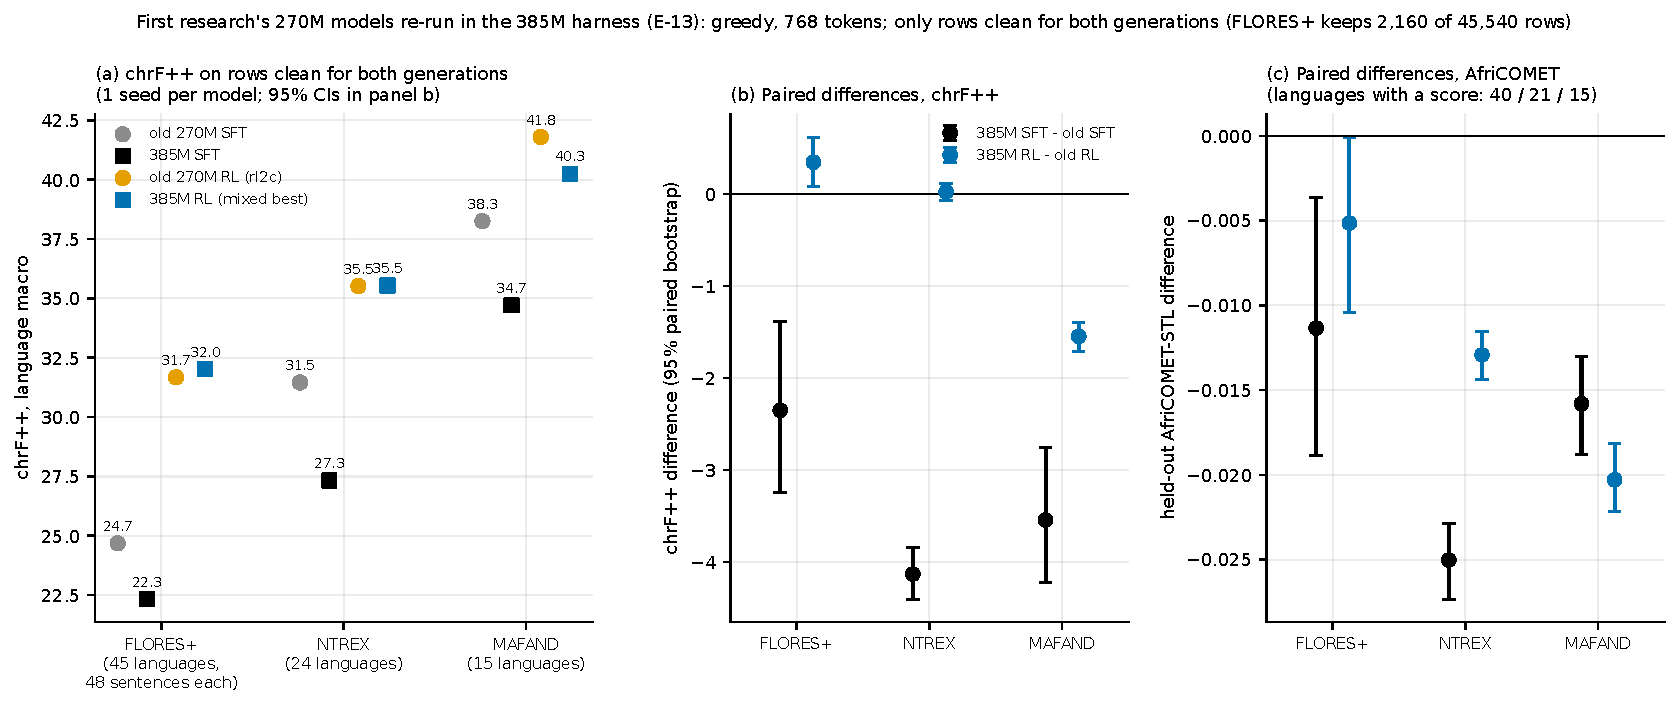
\includegraphics[width=1.00\linewidth]{figures/fig10_old270m_same_harness.pdf}
\caption{The earlier 270M work's 270M models re-run in the 385M harness (E-13): (a) language-macro chrF++ of the old 270M SFT and RL-final (rl2c) and the 385M SFT and RL (mixed best) on FLORES+ devtest (45 languages, 48 sentences each), NTREX (24) and MAFAND (15), rows clean for both generations only; (b) paired differences with 95\% bootstrap over sentences (Poisson weights; 1,000 resamples); (c) the same for held-out AfriCOMET-STL (languages with a score: 40 / 21 / 15). One seed per model. Source: \texttt{reports/\allowbreak{}data/\allowbreak{}e13\_\allowbreak{}old270m\_\allowbreak{}same\_\allowbreak{}harness\_\allowbreak{}2026-\allowbreak{}11-\allowbreak{}04/\allowbreak{}evidence\_\allowbreak{}e13.\allowbreak{}json}.}\label{fig:fig10_old270m_same_harness}
\end{figure}

\subsection{Weak and added languages}\label{app:weaklangs}

After SFT, 37 of 74 scored languages are weak (chrF++ < 14 or finished rate < 0.9), 16 of them by chrF++: shi 0.2, ibb 2.3, zgh 2.3, dag 2.4, aeb 2.8, taq 2.8, dik 3.8, knc 3.8, arz 4.6, ary 4.6, dyu 9.9, tir 10.5, cjk 10.7, orm 12.1, tiv 13.3, nus 13.5. Of the nine languages that the SFT report lists as added (the eight on FLORES+ that are among the 40 registry rows appended after A0, plus seh, which the registry counts among the first 85 rows), mfe (28.5) and seh (21.7) work, cjk (10.7) is weak, and arz, ary, dik, aeb, taq and zgh fail (English or Modern Standard Arabic output, token loops).  After RL (mixed best): mfe 37.93, cjk 23.02, dik 14.06, taq 11.06, arz 9.18, ary 6.88, aeb 4.12, zgh 4.07.  Arabic dialects, Tamazight, Dinka, Tamasheq and Kanuri (knc) are not usable after RL (chrF++ 2 to 14; loops in 11\% to 56\% of FLORES+ outputs by the reward's flag, and an English-output share of up to 0.5 in aeb and ary, Section~\ref{sec:degen}).
% src: EVAL section 6, T5
% src: EVID Table 6

\begin{figure}[t]
\centering
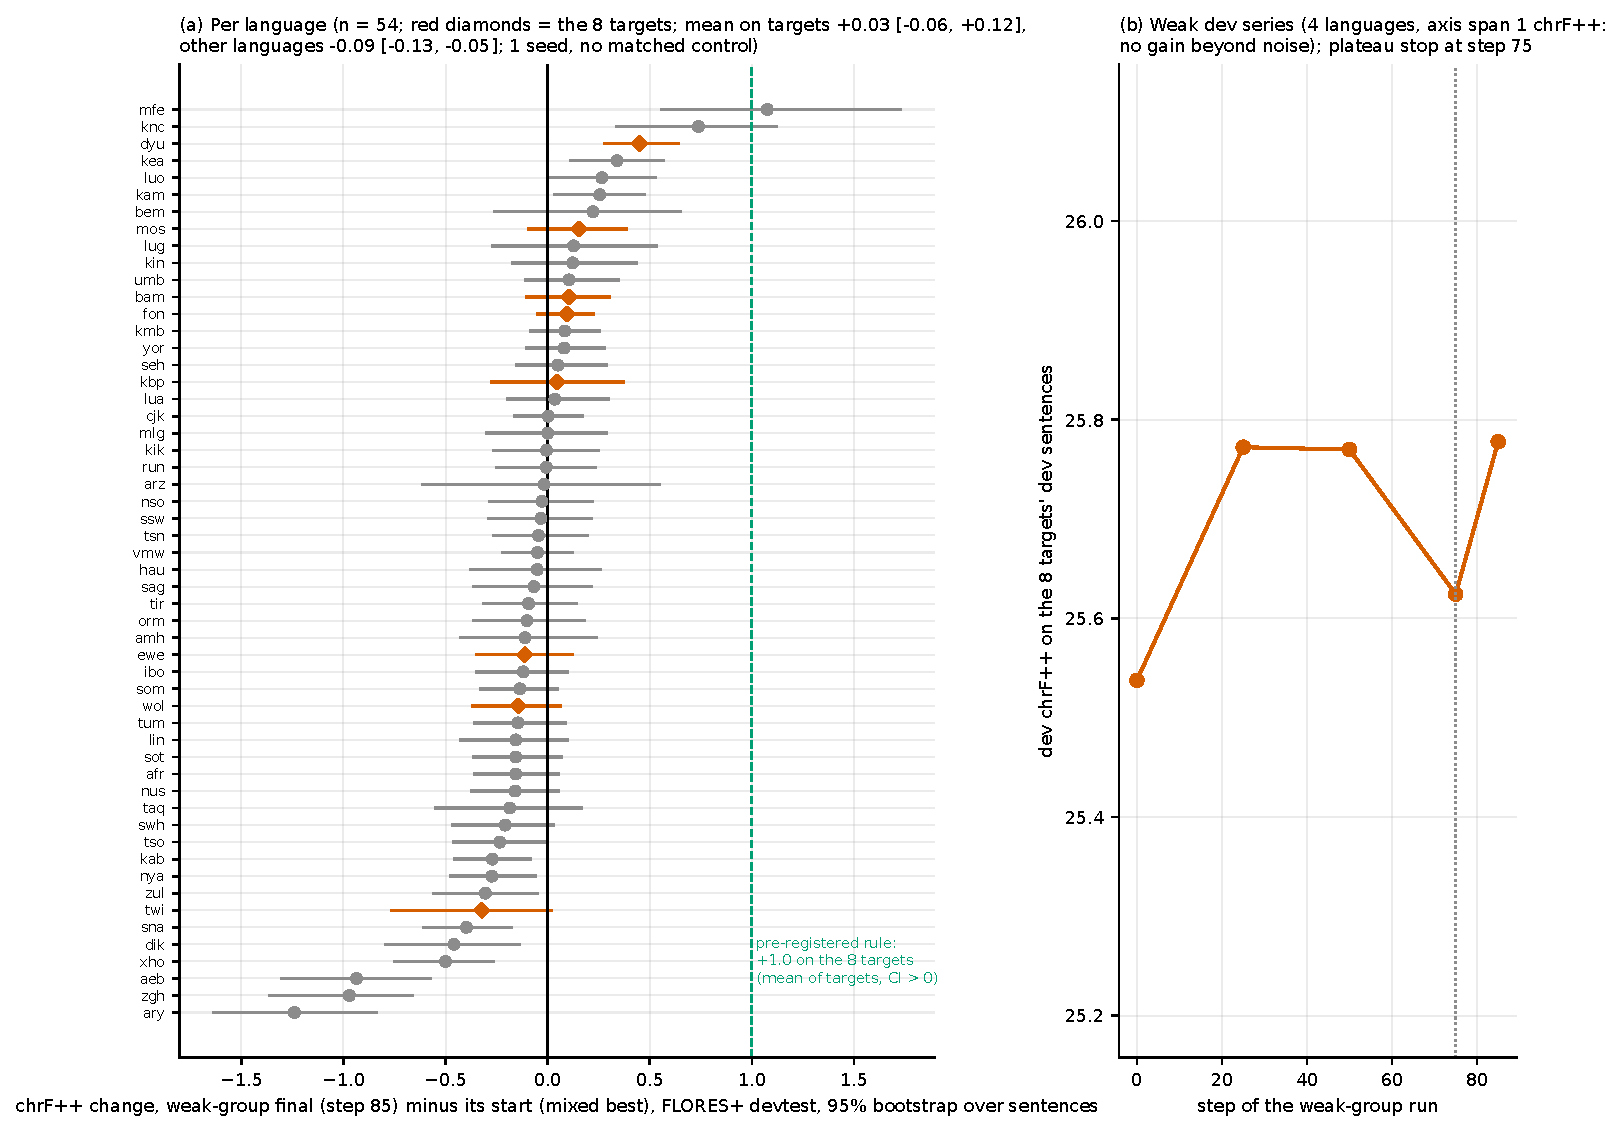
\includegraphics[width=0.90\linewidth]{figures/fig6_weak_group.pdf}
\caption{(a) Continued RL on eight weak West-African languages (mos fon kbp bam wol ewe twi dyu; 85 steps, 2.1 GPU-hours): chrF++ change of the final (step 85) against its start, the mixed best, per FLORES+ language (n = 54; 1,012 sentences each; 95\% bootstrap over sentences; one seed, no matched control). Red diamonds are the targets: mean +0.03 [\ensuremath{-}0.06, +0.12] against the pre-registered +1.0; the 46 other languages move by \ensuremath{-}0.09 [\ensuremath{-}0.13, \ensuremath{-}0.05]. (b) The run's own dev series on the targets' dev sentences (axis span 1 chrF++; dev evaluation noise is sd 0.09 to 0.10). Sources: \texttt{reports/\allowbreak{}data/\allowbreak{}eval\_\allowbreak{}weak\_\allowbreak{}group\_\allowbreak{}2026-\allowbreak{}11-\allowbreak{}03/\allowbreak{}scores/\allowbreak{}bootstrap\_\allowbreak{}by\_\allowbreak{}language.\allowbreak{}csv}, \texttt{research\_\allowbreak{}archive\_\allowbreak{}2026-\allowbreak{}11-\allowbreak{}03/\allowbreak{}clean\_\allowbreak{}rerun\_\allowbreak{}misc/\allowbreak{}runs\_\allowbreak{}385m\_\allowbreak{}weak/\allowbreak{}mixed/\allowbreak{}metrics.\allowbreak{}jsonl}.}\label{fig:weakgroup}
\end{figure}

\section{RL chain: stage summary, B1 final and training records}\label{app:chain}

\begin{table}[t]
\centering\scriptsize
\setlength{\tabcolsep}{4pt}
\caption{Stage chain summary (not all rows are FLORES+ stages).}\label{tab:chain_full}
\begin{tabularx}{\linewidth}{@{}>{\raggedright\arraybackslash}X>{\raggedright\arraybackslash}X>{\raggedright\arraybackslash}X>{\raggedright\arraybackslash}X@{}}
\toprule
stage & steps run & cost & result on FLORES+ chrF++ (vs previous stage) \\
\midrule
SFT-1 / SFT-2 (A0 $\to$ 385M) & 1,500 + 31,353 & 44.8 h for stage B (A100) & 22.85 (SFT, 54 languages) \\
continued-SFT control (E-03; not an RL stage) & 6,000 & 8.4 h (5.05 s/step), RL chain 8.66 h & FLORES+ 25.38 (+2.53 over the SFT [+2.35, +2.71]); 93 cells 29.97 against 34.55 for the mixed best \\
RL stage A & 400 & 15,920 s (4.42 h) & 30.81 (+7.96) \\
RL B1 & 135 (best step 50) & 10,479 s & 31.35 (+0.54) \\
RL mixed & 60 & 4,786 s & 31.66 (+0.31) \\
weak-group RL (8 languages) & 85 (plateau stop at 75) & 2.1 GPU-h & targets +0.03 [\ensuremath{-}0.06, +0.12]; other languages \ensuremath{-}0.09 [\ensuremath{-}0.13, \ensuremath{-}0.05] \\
science SFT & 283 (65,536 tokens) & 17 min & AfriScience chrF +1.2; SSA-COMET-QE flat \\
science RL & 160 steps executed (cap 150 in the yaml, extended to 190 at step 120; dev plateau at step 150 plus 10 wind-down steps; \texttt{summary.\allowbreak{}json} stop reason \texttt{dev\_\allowbreak{}plateau}; best at step 75) & not stated in the evaluation report & AfriScience test (6 languages), final vs start: chrF +0.46 [+0.27, +0.65], held-out AfriCOMET +0.0053 [+0.0036, +0.0071], SSA-COMET-QE +0.0041 (reward family); NTREX +0.42, MAFAND +0.10 chrF++; no document-level gain (not a FLORES+ stage) \\
science RL without the science SFT (E-14) & 160 (150 + 10 wind-down; one OOM restart from step 20; final only) & about 5 h wall-clock (15:18 to 20:17 UTC; 14,395 s in the last process) & AfriScience test chrF 45.66 (start 45.40; science RL from the science SFT 47.10); 93-cell chrF++ +0.13 over the mixed best (not a FLORES+ stage) \\
long-document RL & 80 (best at step 50; no extension) & 7.7 h wall-clock, of which about 4.5 h a crash loop (Appendix~\ref{app:repro}) & whole-document finished +0.125, loop \ensuremath{-}0.113, chrF +3.4; chunked and sentence level unchanged (not a FLORES+ stage) \\
\bottomrule
\end{tabularx}
\end{table}

% GATE E-03: the cost column is the compute the control must match
% src: reports/rl_vs_sft_evidence_2026-11-04.md section 6 (cost); EVID Table 3; reports/eval_weak_group_385m_2026-11-03.md; reports/eval_science_sft_385m_2026-11-04.md; LDOC section 2 (planned values). Science RL length: the yaml labels 150 steps a HARD CAP, but `extend_if_improving` (the trainer's extension rule: at the cap, if the improvement criterion fired within the last `extend_recent` steps, raise the cap) raised it by 40 steps to 190 while the dev metrics were still improving; the long-document yaml sets `extend_if_improving: false`. The stage A to mixed yamls also carry the extension rule (extend_steps 15, at most +50%). The executed count is reported from the run log and must be confirmed from `summary.json` when the run ends. The RL chain A + B1 + mixed is 8.66 A100-hours, of which B1's 85 steps after its best checkpoint are unused by the final model

 Stage A accounts for 94\% of the SFT-to-B1 gain on FLORES+ (7.96 of 8.50) and 96\% on NTREX; it also accounts for most of the improvement in finishing and looping (FLORES+ finished 0.829 $\to$ 0.983, loop 0.209 $\to$ 0.068; final 0.995, 0.048; Section~\ref{sec:rlsft}). We did not split the part beyond finishing by stage. The stage-A dev chrF++ (720 sentences) moves 36.81 $\to$ 39.04 (step 50) $\to$ 40.14 (100) $\to$ 40.47 (200) $\to$ 40.50 (400), with +3.3 of +3.7 in the first 100 steps; the plateau begins before the three KL-guard cuts (steps 226, 236, 247).  The later stages differ from stage A in more than step count (bin, reference domain, guides), and the later steps are small. Two extra seeds of the stage-A recipe (E-04, 100 steps, 20 languages, standard harness; Appendix~\ref{app:split}) differ by 0.06 chrF++ [\ensuremath{-}0.02, +0.14] (0.0008 AfriCOMET). On those 20 languages the stored B1 best is +0.17 [+0.12, +0.21] chrF++ over stage A, about three times the seed difference, while the mixed best is +0.07 [+0.02, +0.11] over B1 best, the size of the seed difference: \textbf{we do not call the mixed step a gain}; stage A to mixed is +0.23 [+0.18, +0.29]. These are indications from one pair of seeds at step 100, not tests of the later stages. 
% src: EVID Table 3; arithmetic checked in HYG X16
% src: STA; HYG X4
% src: reports/e04_rl_seeds_2026-11-05.md section 2; ledger E04 rows

\textbf{B1 best against B1 final (E-20).} The B1 final weights (step 135; \anonreal{an anonymised checkpoint}{Hub branch \texttt{stage-\allowbreak{}b1-\allowbreak{}final}}) were evaluated on the same 122,585 rows as every other stage (greedy, 768 tokens, language macro, 95\% paired bootstrap, one seed). 
% src: reports/e20_b1_final_2026-11-04.md; reports/data/e20_b1_final_2026-11-04/evidence_e20.json (ledger M8b)

\begin{table}[t]
\centering\footnotesize
\setlength{\tabcolsep}{4pt}
\caption{B1 final (step 135) against B1 best (step 50) and neighbouring stages; \chrfpp{}, language macro, 95\% paired bootstrap.}\label{tab:e20}
\begin{tabularx}{\linewidth}{@{}>{\raggedright\arraybackslash}Xllll@{}}
\toprule
comparison & FLORES+ chrF++ & NTREX chrF++ & MAFAND chrF++ & all 93 cells chrF++ \\
\midrule
B1 final minus B1 best & +0.04 [+0.00, +0.08] & \ensuremath{-}0.00 [\ensuremath{-}0.05, +0.05] & \ensuremath{-}0.09 [\ensuremath{-}0.15, \ensuremath{-}0.01] & +0.01 [\ensuremath{-}0.02, +0.04] \\
B1 final minus stage A & +0.58 [+0.53, +0.64] & +0.30 [+0.24, +0.36] & \ensuremath{-}0.09 [\ensuremath{-}0.17, +0.00] &  \\
mixed best minus B1 final & +0.26 [+0.22, +0.30] & +0.19 [+0.14, +0.23] & +0.05 [\ensuremath{-}0.01, +0.12] &  \\
\bottomrule
\end{tabularx}
\end{table}

Held-out AfriCOMET, B1 final minus B1 best, all cells: +0.0004 [+0.0000, +0.0008]; FLORES+ finished / loop 0.993 / 0.054 (B1 best) and 0.996 / 0.052 (B1 final). The 85 steps after step 50 changed nothing measurable, so the choice between B1 best and final does not matter for the numbers of this paper; 11 of 93 cells are significantly worse and 8 significantly better, by 0.1 to 0.3 chrF++, which is a rough noise floor for the stage-to-stage steps. (A table, not a figure, because the content is three differences.)

\begin{figure}[t]
\centering
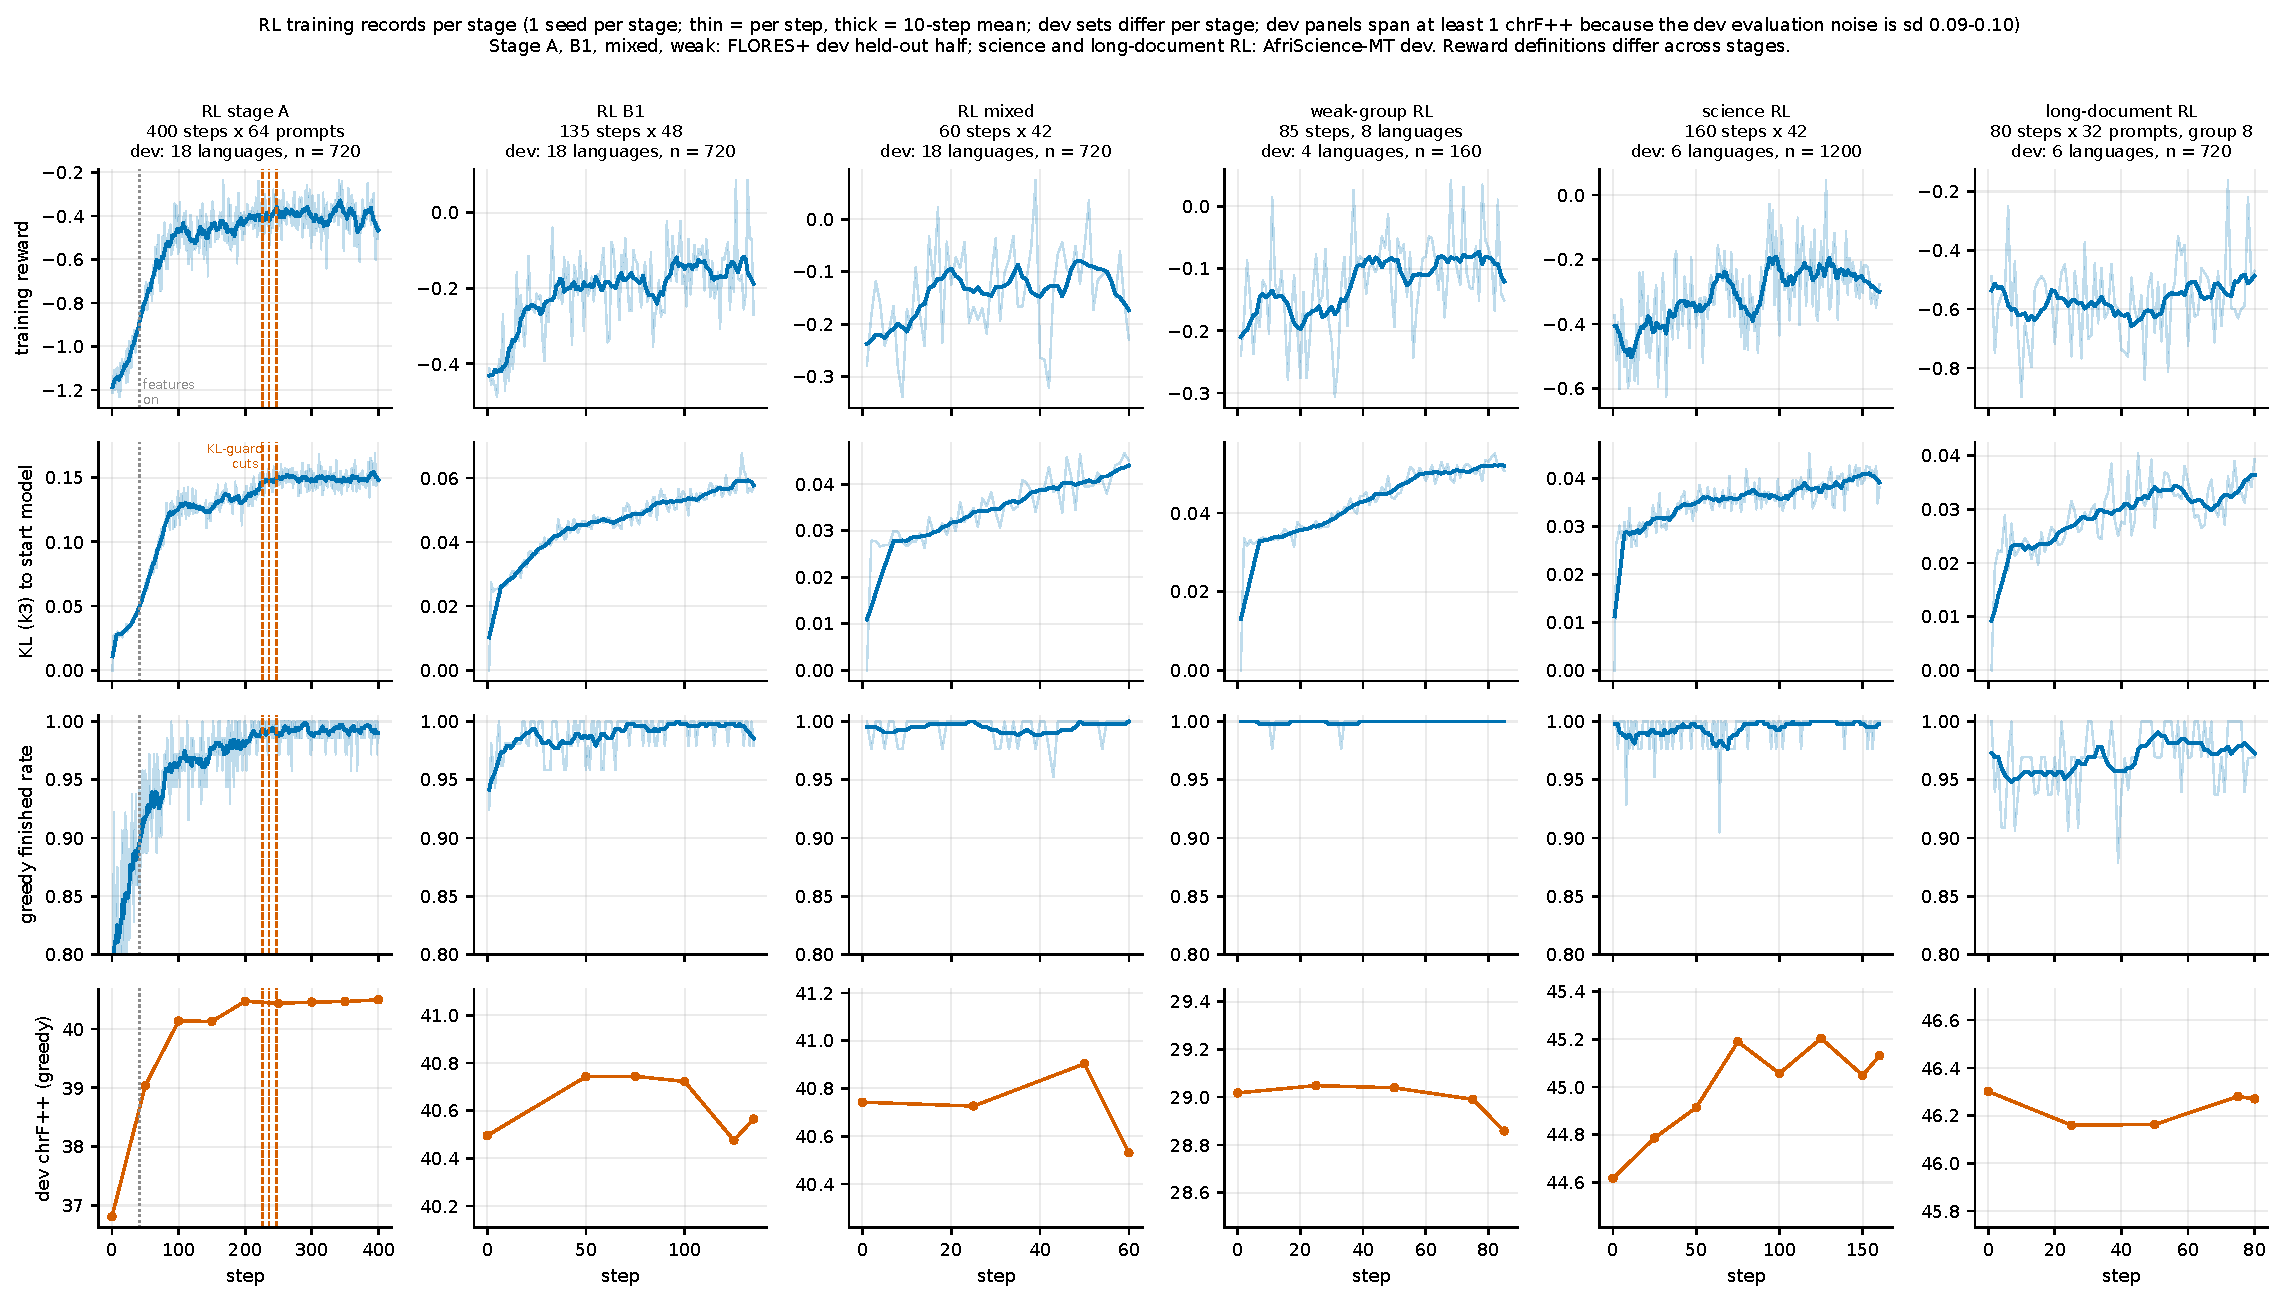
\includegraphics[width=1.00\linewidth]{figures/fig2_rl_training_curves.pdf}
\caption{Training records of every RL stage from the run logs (one seed per stage): training reward, KL (k3) to the stage's start model, finished rate of the greedy group member, and dev chrF++ against the step (thin lines per step, thick lines 10-step means). Stage A: dotted line at step 41 (four features on), dashed lines at the three KL-guard cuts (226, 236, 247). The dev sets differ by stage (FLORES+ dev held-out half for stage A, B1, mixed and weak; AfriScience-MT dev for science and long-document RL; the number of languages and sentences is in each title) and the reward definitions differ, so columns are not comparable; dev panels span at least 1 chrF++ because the dev evaluation noise is sd 0.09 to 0.10. The long-document RL log shows the 80 planned steps; step 25 was evaluated repeatedly after the crash restarts of Appendix~\ref{app:repro} and the last evaluation is shown (steps 21 to 25 were repeated by the restarts). Sources: \texttt{research\_\allowbreak{}archive\_\allowbreak{}2026-\allowbreak{}11-\allowbreak{}03/\allowbreak{}runs\_\allowbreak{}385m/\allowbreak{}\{A,B1,mixed\}/\allowbreak{}metrics.\allowbreak{}jsonl}, \texttt{clean\_\allowbreak{}rerun\_\allowbreak{}misc/\allowbreak{}runs\_\allowbreak{}385m\_\allowbreak{}\{weak/\allowbreak{}mixed,sci/\allowbreak{}final,long/\allowbreak{}final\}/\allowbreak{}metrics.\allowbreak{}jsonl}.}\label{fig:fig2_rl_training_curves}
\end{figure}

\section{RL against SFT and the control: details}\label{app:rlsft}

\begin{table}[t]
\centering\footnotesize
\setlength{\tabcolsep}{4pt}
\caption{Finished rate / loop rate (reward's flag) / hypothesis-to-reference length, clean rows, language macro.}\label{tab:finish}
\begin{tabularx}{\linewidth}{@{}l>{\raggedright\arraybackslash}Xll@{}}
\toprule
system & FLORES+ finished / loop / hyp-to-ref length & NTREX & MAFAND \\
\midrule
SFT & 0.829 / 0.209 / 3.03 & 0.890 / 0.122 / 2.35 & 0.963 / 0.043 / 1.48 \\
RL stage A & 0.983 / 0.068 / 1.33 & 0.996 / 0.016 / 1.07 & 0.999 / 0.003 / 1.00 \\
RL B1 best & 0.993 / 0.054 / 1.17 & 0.999 / 0.009 / 1.02 & 1.000 / 0.001 / 0.99 \\
RL mixed best & 0.995 / 0.048 / 1.14 & 0.999 / 0.006 / 1.02 & 1.000 / 0.001 / 0.98 \\
\bottomrule
\end{tabularx}
\end{table}

 The loop detector in this table is the reward's own guard (\texttt{is\_\allowbreak{}repetitive}, \texttt{is\_\allowbreak{}self\_\allowbreak{}repetitive}); on the human references it fires on 0.0001 of FLORES+ rows. 95\% of the RL model's flagged FLORES+ rows come from seven near-failed languages (taq knc zgh dik aeb arz ary). Section~\ref{sec:degen} tests this flag against a detector that is not the reward's.
% src: EVID Table 2

\begin{table}[t]
\centering\footnotesize
\setlength{\tabcolsep}{4pt}
\caption{RL minus SFT over the 93 cells under four ways of removing the finishing effect (clean rows; 95\% CI).}\label{tab:decomp}
\begin{tabularx}{\linewidth}{@{}>{\raggedright\arraybackslash}X>{\raggedright\arraybackslash}X>{\raggedright\arraybackslash}X@{}}
\toprule
row set & chrF++ RL - SFT [95\% CI] & AfriCOMET RL - SFT [95\% CI] (76 cells) \\
\midrule
all clean rows & +7.96 [+7.82, +8.12] & +0.0631 [+0.0620, +0.0643] \\
SFT output cut at its first loop (RL as is) & +4.06 [+3.97, +4.15] & not scorable \\
rows where the SFT finished and did not loop & +2.41 [+2.33, +2.49] & +0.0366 [+0.0357, +0.0374] \\
rows where both finished and neither loops & +2.61 [+2.54, +2.70] & +0.0370 [+0.0362, +0.0379] \\
rows where the SFT failed (21\% of FLORES+ rows) & +24.57 [+24.26, +24.90] (SFT 5.95, RL 30.53) & +0.3342 [+0.3295, +0.3391] \\
\bottomrule
\end{tabularx}
\end{table}

 Cutting the SFT's looping outputs at the loop onset (no change to the translation) raises the SFT from 26.59 to 30.49 chrF++, i.e. \textbf{49\% of the gain is recovered by cutting loops}; 67 to 70\% of the chrF++ gain is attributable to rows where either model failed; about 41\% of the AfriCOMET gain is finishing. What remains is +2.4 to +4.1 chrF++ and +0.037 AfriCOMET, significant in 50 of 54 FLORES+ languages on clean rows. The three estimates favour different models (the paired subset keeps only sentences the SFT can handle; the cut-at-loop rule is a heuristic) and agree in sign and rough size. The cut-at-loop rule is the reward family's loop rule; it was not redone with the independent detector of Section~\ref{sec:degen}. The decode-time guard control (E-01, below) answers the question this raises: a frequency penalty of 0.10 on the SFT recovers the same 49\% of the chrF++ gain (29\% of the AfriCOMET gain) without any RL, so the finishing share is a property of unguarded greedy decoding that the RL also repairs. Caveats: the guard setting was chosen on the FLORES+ dev held-out half by a rule fixed in advance and its optimum (0.10) lay at the edge of the grid, so the control may be under-tuned; a post-hoc dev-only extension to stronger penalties (SFT dev chrF++ 37.36 at 0.10, 37.97 at 0.20, 38.00 at 0.30, 38.25 at 0.50) was still rising and no full evaluation with a stronger penalty was run; one seed (\texttt{reports/\allowbreak{}e01\_\allowbreak{}loop\_\allowbreak{}guard\_\allowbreak{}2026-\allowbreak{}11-\allowbreak{}04.\allowbreak{}md}, \texttt{reports/\allowbreak{}overnight\_\allowbreak{}log\_\allowbreak{}2026-\allowbreak{}11-\allowbreak{}04.\allowbreak{}md} 09:00 row).
% src: EVID Table 1, section 3

Language-macro chrF++ per benchmark, SFT / control / mixed best: FLORES+ 22.85 / 25.38 / 31.66, NTREX 29.25 / 33.74 / 37.17, MAFAND 35.77 / 40.44 / 40.78; the control gains +2.53 [+2.35, +2.71], +4.49 [+4.29, +4.70] and +4.67 [+4.39, +4.92] over the SFT against +8.81, +7.91 and +5.01 for the RL; over the 93 cells it gains +3.38 against +7.96 (42.5\% of the SFT-to-RL gap, arithmetic of the macros). Held-out AfriCOMET: RL minus control is +0.0373 on FLORES+, +0.0051 on NTREX and \ensuremath{-}0.0141 on MAFAND (the last favours the control). Finished and loop rates (the reward's flag) on FLORES+, SFT / control / mixed best: 0.829 / 0.854 / 0.995 and 0.209 / 0.178 / 0.048; by panel (FLORES+ finished): the 19 TranslatePsy languages 0.931 / 0.993 / 1.000, the other languages 0.774 / 0.779 / 0.993. The independent degeneration detector gives the same picture (FLORES+ flag 0.311 for the SFT, 0.268 for the control, 0.085 for the mixed best). \textbf{The control repairs finishing and looping only on the languages it was trained on}, where it comes close to the RL model; on the other languages it changes almost nothing (+0.15 chrF++ over the SFT on FLORES+ [\ensuremath{-}0.03, +0.32], 35 languages). 

\begin{table}[h]
\centering\small
\caption{The pre-registered decision rule applied to mixed best against the 6,000-step control.}\label{tab:e03rule}
\begin{tabular}{@{}llc@{}}
\toprule
registered condition & value & met\\
\midrule
lower 95\% bound of $d$ (\chrfpp{}, 93 cells) $>+1.0$ & $+4.58$ \ci{+4.45}{+4.70} & yes\\
lower bound of the AfriCOMET difference $>0$ & $+0.0183$ \ci{+0.0172}{+0.0192} & yes\\
$d>0$ on the 19 TranslatePsy languages & $-0.03$ \ci{-0.13}{+0.09} & \textbf{no}\\
$d>0$ on the other languages & $+9.29$ \ci{+9.09}{+9.49} & yes\\
\bottomrule
\end{tabular}
\end{table}

\textbf{By the rule as registered the verdict is ``inconclusive''}, because the condition on the 19 TranslatePsy languages is not met (d = \ensuremath{-}0.03); the other three are. We did not change the rule. Reading the panels: where a teacher-translated corpus exists continued SFT matches RL in chrF++ and largely fixes finishing and looping, and the control is ahead of RL on the neural metrics there; RL's advantage is that it improves every language from its own samples and a QE reward, including those for which no such corpus was used (+9.29 on 46 cells). A reader who takes the overall endpoint alone gets ``RL is better'' (+4.58 [+4.45, +4.70], above the +1.0 margin, AfriCOMET above 0); a reader who takes the 19 languages alone gets ``comparable'' in chrF++ (interval inside $\pm$1.0) but not by the registered rule (the AfriCOMET interval excludes 0 in favour of the control); neither is the registered verdict. On AfriScience-MT test sentences (6 languages) the control scores chrF 44.71 against 45.40 for the mixed best and 36.00 for the SFT, and is ahead of the RL on SSA-COMET-QE (0.6214 against 0.6130) and AfriCOMET (0.6947 against 0.6828), the metrics in the family that filtered TranslatePsy; nso, the one of the six languages without TranslatePsy data, stays at the SFT level for the control (41.27 $\to$ 40.64) while the RL gains 10.9.

Caveats. One seed, \textbf{one learning rate} (the probe's best of three) and \textbf{one evaluated budget point}: the stage-A-matched (3,100 steps) and mixed-best-matched (4,800 steps) comparisons are untested, and a different mix, schedule or longer run could change the control. Differences below about 0.5 chrF++ are inside the unmeasured seed variation. The control is not information-matched: it receives NLLB-3.3B translations (a teacher that scores 38.80 against 26.30 for the SFT on 43 languages, Section~\ref{sec:nllb}) for 19 languages that the RL never sees, and the TranslatePsy rows were filtered with AfriCOMET, SSA-COMET and MetricX, so those neural metrics favour the control; chrF and chrF++ are the evidence. The control's loop count is undercounted by the reward's flag too (independent / reward flag 1.51 on FLORES+). TranslatePsy is CC-BY-NC-4.0 with NLLB-derived targets and was used only for this control; nothing of it is in any released model, and the control checkpoint is not released (Appendix~\ref{app:disc}). 
% src: reports/e03_sft_control_2026-11-05.md sections 1, 3, 4; ledger R14, CTL7-CTL11

\section{Independent degeneration audit: details}\label{app:degenapp}

The reward's loop flag is the guard the RL was optimised against, so a loop type it misses would be undercounted for the RL. We re-measured with a detector that shares the idea (repetition) but none of the code or constants: the lzma-compressed size of the output relative to what human references of the same benchmark, language and length would give, the share of repeated character 8-grams and the share of repeated word 3-grams, each threshold set so that 0.1\% of the 122,585 human references fire it. Rows are all rows of FLORES+ (54 languages), NTREX (24) and MAFAND (15) for each system, no clean-row filter.  
% src: DEGEN section 2 Table; `reports/data/degeneration_audit_independent_2026-11-04/summary_by_model_benchmark.csv`, `bootstrap_rates.csv`. DEGEN uses all rows while EVID Table 2 uses clean rows; the reward-flag values agree to the three decimals quoted in EVID (0.209/0.048, 0.122/0.006, 0.043/0.001)

\begin{table}[t]
\centering\footnotesize
\setlength{\tabcolsep}{4pt}
\caption{Loop flag of the reward against the independent detector, language macro (95\% bootstrap in brackets).}\label{tab:degen}
\begin{tabularx}{\linewidth}{@{}lrrl>{\raggedright\arraybackslash}X@{}}
\toprule
system & FLORES+ reward flag & FLORES+ independent flag & NTREX reward / independent & MAFAND reward / independent \\
\midrule
SFT & 0.2095 & 0.3107 [0.3029, 0.3190] & 0.1218 / 0.1662 & 0.0431 / 0.0754 \\
RL stage A & 0.0675 & 0.1207 [0.1160, 0.1253] & 0.0165 / 0.0309 & 0.0026 / 0.0092 \\
RL B1 best & 0.0541 & 0.0980 [0.0942, 0.1019] & 0.0092 / 0.0190 & 0.0013 / 0.0056 \\
RL mixed best & 0.0480 [0.0462, 0.0496] & 0.0851 [0.0822, 0.0883] & 0.0064 / 0.0143 & 0.0009 / 0.0039 \\
human references & 0.0001 & 0.0018 & 0.0000 / 0.0018 & 0.0000 / 0.0013 \\
\bottomrule
\end{tabularx}
\end{table}

\begin{itemize}
\item \textbf{The reward's flag is a lower bound.} On mixed-best FLORES+ the independent detector flags 1.77 [1.71, 1.84] times as many outputs as the reward's flag (NTREX 2.25 [1.95, 2.59], MAFAND 4.42 [3.14, 7.29] on tiny base rates). At a ten times stricter threshold (0.01\% of references) the FLORES+ rates are 0.0586 against 0.0480 (ratio 1.22), so the excess is not an artefact of a loose threshold. The undercount is present for the SFT too (ratio 1.48), so it enters the RL-versus-SFT comparison only through 1.48 against 1.77; the reduction of the loop rate from SFT to RL is 3.7x with the independent detector and 4.4x with the reward's.
\item \textbf{The extra rows are finished partial repetitions and cost little.} Of 122,585 mixed-best rows, 2,932 are flagged by both, 14 by the reward only and 2,488 by the independent detector only. The independent-only rows are 99.9\% finished, have a median of 26 words and 48\% of them are in the seven near-failed languages. Hard failures are caught by both (of 278 unfinished rows 2 escape the reward's flag and none the independent one). If the independent-only rows scored the average of the unflagged rows of their language, the macro chrF++ of the mixed best would rise by 0.19 (FLORES+), 0.02 (NTREX) and 0.015 (MAFAND), against 0.46, 0.28 and 0.23 for the SFT. The difference between SFT and RL in this loss is 0.26, 0.26 and 0.22 chrF++, i.e. 3.0\%, 3.3\% and 4.4\% of the RL gains (+8.81, +7.91, +5.01) by arithmetic. \textbf{The decomposition above does not change materially.} 
% src: DEGEN section 0, `crosstab_reward_vs_independent.csv`, `chrf_loss_attributable_to_independent_only_rows.csv`. The language-matched chrF++ of independent-only rows is 4.54 below that of unflagged rows (se 0.51; 39 of 44 languages) but this is selection-confounded (hard sentences repeat more). DISAGREEMENT FLAG: the report's "3 to 4%" rounds 4.4% down; use the three percentages
\item \textbf{Length and tails.} Median hypothesis-to-reference character ratio is 1.02 to 1.07 for all systems. The share of FLORES+ outputs longer than twice the reference falls from 0.2005 (SFT) to 0.0281 (mixed best). Of the 2,079 mixed-best rows above 2x, 24.5\% (about 0.4\% of all rows) are finished and flagged by neither detector: long, non-repetitive continuations that no repetition rule sees. Unterminated tails on FLORES+ fall from 0.1847 to 0.0464 against 0.0162 for human references; NTREX and MAFAND are at or below the reference rate. 
% src: DEGEN sections 3, 4
\item \textbf{Language.} An independent language-identification model (NLLB-218, reliable for 40 of the evaluated languages) agrees with the reward's GlotLID: FLORES+ pass rate SFT 0.9487, mixed best 0.9669 (references 0.9915); GlotLID 0.9098 and 0.9553. On mixed-best FLORES+ 0.86\% of the rows GlotLID passes fail the NLLB LID, so the language guard's pass rate is not inflated by optimisation. The LID is blind to the weakest languages (none for aeb ary arz mfe nde seh shi ven vmw; unreliable for nine more). 
% src: DEGEN section 6
\end{itemize}

 Four languages account for 96\% of the macro increase (human references: 0.0004); GlotLID gives the same numbers within 0.005. These languages, with taq, dik and knc, are outside the RL prompt pool, and the model emits the tag of a sibling language (\texttt{<arz>} for ary and half of aeb, \texttt{<tzm>} for zgh and taq). The reward's copy guard sees only 0.086 of aeb and 0.064 of ary outputs. So part of the ``RL loops less'' gain in these languages is a change from loops to English output, while their chrF++ stays at 2 to 9.
% src: DEGEN section 5, `arabic_tifinagh_english_leak.csv`
\begin{itemize}
\item \textbf{What the audit does not establish.} There is no ground truth for ``degenerate''; the detector is validated by the reference control, by reading 25 mixed-best and 12 SFT examples, and by the lower language-matched chrF++. It is blind to non-repetitive failures (hallucination, wrong content) except through the length audit. The NLLB LID is licensed cc-by-nc-4.0 and was used for evaluation only.
\end{itemize}

The share of outputs identified as English (NLLB-218 top-1, $p\ge0.5$) on FLORES+ by system:

\begin{table}[t]
\centering\small
\setlength{\tabcolsep}{4pt}
\caption{Share of FLORES+ outputs identified as English, by system.}\label{tab:english}
\begin{tabularx}{\linewidth}{@{}>{\raggedright\arraybackslash}Xrrrrr@{}}
\toprule
language & SFT & stage A & B1 best & mixed best & weak final \\
\midrule
aeb & 0.215 & 0.400 & 0.397 & 0.449 & 0.498 \\
ary & 0.041 & 0.275 & 0.339 & 0.394 & 0.488 \\
arz & 0.006 & 0.059 & 0.075 & 0.098 & 0.151 \\
zgh & 0.001 & 0.017 & 0.029 & 0.049 & 0.074 \\
macro, 54 languages & 0.0055 & 0.0146 & 0.0164 & 0.0191 & 0.0235 \\
\bottomrule
\end{tabularx}
\end{table}

\section{Stage-A log analysis and ablation details}\label{app:split}

\textbf{The stage-A log cannot separate the four features (E-11 can).} Stage A steps 1-40 ran without the four features and steps 41-400 with them. An earlier note said the KL slope ``tripled'' when the features began (0.00053 per step over steps 2-40, 0.00143 over steps 41-100). Reading the log: both numbers reproduce exactly, \textbf{but the factor is 2.0, not 3}: the first segment contains the learning-rate warm-up (steps 1-10); from step 11 the pre-feature slope is 0.00070 [0.00061, 0.00079] and 0.00143/0.00070 = 2.0. The KL was also already accelerating before step 41 (slopes over 15-step windows: 0.00048 for steps 11-25, 0.00101 for 26-40, 0.00158 for 41-55), the curve is smooth through step 41 with no kink, and it saturates by step \textasciitilde\{\}90 (flat at 0.124 to 0.129 until step \textasciitilde\{\}160). A power-law extrapolation of the pre-feature trend predicts a KL of 0.042 to 0.065 at step 100 against 0.131 observed, so the acceleration is faster than the extrapolated trend, but that is a statement about extrapolating 30 to 40 noisy points, not an identification of a cause. 
% src: SPLIT sections 1-2; ledger R17

\textbf{Nothing else accelerates at step 41.} The per-step slopes of the training reward (+0.0065 [0.0051, 0.0079] before, +0.0071 [0.0060, 0.0080] after), of the finished rate, of the greedy loop rate (\ensuremath{-}0.0020 before, \ensuremath{-}0.0011 after) and of the hard-fail share (\ensuremath{-}0.00138 before, \ensuremath{-}0.00040 after) are the same or steeper before step 41, because the failure rates were high and floor out. An interrupted-time-series fit finds level shifts at step 41 (KL +0.0086 [0.0021, 0.0149], reward +0.093 [0.041, 0.147], greedy loop rate \ensuremath{-}0.028 [\ensuremath{-}0.052, \ensuremath{-}0.004], hard-fail share \ensuremath{-}0.014 [\ensuremath{-}0.026, \ensuremath{-}0.003]), but the reward and the finished and loop rates are not the same quantity before and after step 41 (from step 41, 15\% of the prompts carry the reference term and 25\% of the groups contain the guide), and the shifts could equally be a resume artefact (checkpoint reload, RNG, a fresh prompt stream). They say ``something changed at 41 on top of the trend'', not which feature did it. The dev curve is evaluated only at steps 0, 50, ..., 400, so no dev point separates steps 1-40 from 41-50. 
% src: SPLIT section 2; ledger R18

\textbf{Which feature could act at all.} Dynamic sampling never acted (flat-group fraction 0, no refill) and the std floor never bound (group-std p10 0.128 against 0.02), so any effect at step 41 could only come from the beam guide, the reference domain or the resume itself; the log could not say which. We therefore ran the ablations (below).

\textbf{Seed spread (E-04).} Two extra runs of the stage-A recipe (seeds 20261105 and 20261106; 100 steps; the executed stage A used seed 1234, so the three runs share the recipe, the SFT start and the 40-step feature-free prefix schedule) were evaluated with the standard harness on 20 languages (yor hau ibo swh amh zul xho kin som wol lug sna twi ewe lin tir orm nso tsn afr; FLORES+, NTREX, MAFAND; 49 cells; greedy, 768 tokens). Gains over the SFT are +5.96 [+5.80, +6.11] and +5.90 [+5.74, +6.05] chrF++ (+0.0462 and +0.0454 AfriCOMET): the two seeds differ by \textbf{0.06 chrF++ [\ensuremath{-}0.02, +0.14]} (0.0008 AfriCOMET; per language they differ significantly in 2 of 20, by at most 0.54). The in-training dev gains of the three runs are +3.33, +3.70 and +3.46 (the dev subset depends on the seed, so only gains over each run's own step 0 are compared). The stage-A gain is therefore reproducible across training seeds at step 100, and per-language differences below about 0.5 chrF++ are not separable from training noise. \textbf{This is one pair of seeds at step 100, not a seed study of later stages}; the 400-step stage A is +0.78 [+0.70, +0.86] and +0.84 [+0.75, +0.92] above the 100-step seeds on the same cells. 
% src: reports/e04_rl_seeds_2026-11-05.md sections 1-3 (ledger E04 rows)

\textbf{Ablations (E-11).} Arms (a) no features, (c) no reference domain (no reference prompts and no reference-anchored reward) and (d) no beam guide were run for 100 steps (b64 recipe, one run per arm) as forks of seed 2's step-40 state, so arm minus seed 2 is a tight paired comparison and arm minus seed 3 carries the full seed noise; arm (b), the full set, is the two seeds. Pre-registered rule: an effect is real if the paired interval excludes 0, its size exceeds the observed seed difference (0.06) and AfriCOMET does not point the other way. 

\begin{table}[t]
\centering\footnotesize
\setlength{\tabcolsep}{4pt}
\caption{Ablation arms at 100 steps, \chrfpp{} over 49 cells (20 languages); arm minus the full-feature seed 2 (paired) and minus seed 3 (E-11).}\label{tab:e11}
\begin{tabularx}{\linewidth}{@{}llll>{\raggedright\arraybackslash}X@{}}
\toprule
arm & chrF++ (49 cells) & arm minus seed 2 & arm minus seed 3 & AfriCOMET vs seed 2 \\
\midrule
(b) full, seed 2 & 38.51 [38.30, 38.69] & - & - & - \\
(b) full, seed 3 & 38.46 [38.26, 38.64] & - & - & - \\
(a) no features & 38.19 [37.99, 38.38] & \ensuremath{-}0.32 [\ensuremath{-}0.41, \ensuremath{-}0.23] & \ensuremath{-}0.26 [\ensuremath{-}0.35, \ensuremath{-}0.18] & \ensuremath{-}0.0028 [\ensuremath{-}0.0033, \ensuremath{-}0.0022] \\
(c) no reference domain & 38.35 [38.16, 38.54] & \ensuremath{-}0.16 [\ensuremath{-}0.25, \ensuremath{-}0.08] & \ensuremath{-}0.10 [\ensuremath{-}0.19, \ensuremath{-}0.02] & \ensuremath{-}0.0017 [\ensuremath{-}0.0023, \ensuremath{-}0.0011] \\
(d) no beam guide & 38.42 [38.23, 38.61] & \ensuremath{-}0.09 [\ensuremath{-}0.17, \ensuremath{-}0.01] & \ensuremath{-}0.04 [\ensuremath{-}0.11, +0.04] & \ensuremath{-}0.0005 [\ensuremath{-}0.0010, +0.0001] \\
\bottomrule
\end{tabularx}
\end{table}

Removing all four features costs \textbf{0.32 chrF++ [0.23, 0.41]} (about five times the seed difference; consistent on the three benchmarks, AfriCOMET and the loop flag), about 5\% of the 5.96 chrF++ gain, and it does not show on the in-training dev macro (\ensuremath{-}0.14 [\ensuremath{-}0.51, +0.25]). Removing the reference domain costs 0.16 [0.08, 0.25] (real by the rule against seed 2, 2.7 times the seed difference): about half of the feature set's effect. Removing the beam guide costs 0.09 against seed 2 but 0.04 [\ensuremath{-}0.04, +0.11] against seed 3 with AfriCOMET inside noise: \textbf{not separable from seed noise}, for about +25\% step time (median step 40.3 s with the guide against 32.4 s without). Dynamic sampling and the std floor never acted and are part of arm (a) only. \textbf{The KL rise is not caused by the features:} the median KL of steps 81 to 90 is 0.116 without any feature, 0.122 without the reference domain, 0.120 without the guide and 0.123 and 0.120 for the two full runs, and the same holds at steps 51 to 60 (0.075, 0.0745, 0.073, 0.072, 0.073). \textbf{The earlier inference that the beam guide drives the KL slope (stage report, ledger M10) is therefore not supported}; the step-41 acceleration seen in stage A is at most a small effect. Arm (e) (KL guard 0.25 against 0.15) was not run by the pre-registered rule, because the guard never fired in any of the 100-step runs (maximum 5-step median KL 0.120 to 0.127 against 0.15). Caveats: one run per arm, a shared 40-step prefix with seed 2, one pair of seeds as the noise yardstick (so the ``real'' rule is lenient and effects of 0.1 to 0.2 chrF++ are small and suggestive), 100 steps and 20 languages only (the reference domain covers amh efi hau lug nso yor zul, five of them in these 20). \textbf{Reading:} the four features are design choices with a small measured benefit (+0.3 chrF++ at 100 steps, mostly the reference-anchored term), not the source of the RL gain, and the beam guide is not shown to be worth its generation time. 
% src: reports/e11_rl_ablations_2026-11-05.md sections 1-3 (ledger E11 rows, M10 corrected)

\section{Decoding and engine parity: details}\label{app:decoding}

\textbf{Earlier 256-token study (SFT only; superseded for beam).} 20 languages $\times$ 200 FLORES+ devtest sentences, 256-token cap. Its beam rows came from a vLLM beam loop that completes a beam only on the tokenizer's \texttt{<eos>}, not on \texttt{<end\_\allowbreak{}of\_\allowbreak{}turn>}, and ran every instance to the cap, so \textbf{its beam numbers are not comparable with the beam-4 of E-02 below} and are kept only as the record of what that study measured; its greedy and MBR rows are not affected by this. 
% src: EVAL section 1, T8; reports/e02_beam_mbr_768_2026-11-05.md Amendment 1 and section 4

\begin{table}[t]
\centering\footnotesize
\setlength{\tabcolsep}{4pt}
\caption{Earlier 256-token study (SFT only; 20 languages $\times$ 200 FLORES+ sentences). Beam rows are not comparable with E-02.}\label{tab:old256}
\begin{tabular}{@{}lrlrl@{}}
\toprule
decoding & chrF++ & delta vs greedy [95\% CI] & spBLEU & delta spBLEU \\
\midrule
greedy & 35.00 & - & 13.64 & - \\
beam 4 & 37.53 & +2.53 [+2.18, +2.87] & 16.38 & +2.73 [+2.39, +3.08] \\
MBR-16 (+ greedy) & 38.29 & +3.30 [+3.00, +3.58] & 15.30 & +1.65 [+1.38, +1.90] \\
\bottomrule
\end{tabular}
\end{table}

MBR minus beam is +0.76 [+0.49, +1.02] chrF++ and \ensuremath{-}1.08 [\ensuremath{-}1.39, \ensuremath{-}0.79] spBLEU; MBR uses chrF++ as its utility. The study's greedy is cap-protected (greedy on the same sentences is 32.50 at 768 tokens against 35.00 at 256), which is one more reason not to use its beam gain.

\begin{table}[t]
\centering\scriptsize
\setlength{\tabcolsep}{4pt}
\caption{E-02: greedy, beam-4 and MBR-16 at 768 new tokens, full table (20 languages, 4,000 sentences per system, 95\% paired bootstrap).}\label{tab:e02_full}
\begin{tabularx}{\linewidth}{@{}>{\raggedright\arraybackslash}Xllllll@{}}
\toprule
system & chrF++ & spBLEU & AfriCOMET-STL & finished & loop (independent) & output / reference length \\
\midrule
SFT greedy & 32.31 [31.43, 33.38] & 11.47 & 0.5513 [0.5403, 0.5621] & 0.915 & 0.147 & 2.05 \\
SFT beam-4 (stop at 4 ended) & 36.02 [35.13, 36.95] & 16.49 & 0.5639 [0.5521, 0.5750] & 1.000 & 0.108 & 0.96 \\
SFT beam-4 (HF early\_stopping=False) & 33.26 [32.22, 34.46] & 13.07 & 0.5722 [0.5603, 0.5845] & 0.897 & 0.139 & 2.15 \\
SFT MBR-16 (metric-matched) & 38.27 [37.60, 39.01] & 15.25 & 0.5780 [0.5687, 0.5870] & 0.9998 & 0.016 & 1.16 \\
RL greedy & 39.87 [39.17, 40.62] & 17.39 & 0.6082 [0.5991, 0.6172] & 1.000 & 0.007 & 1.05 \\
RL beam-4 (stop at 4 ended) & 39.10 [38.20, 39.96] & 17.83 & 0.6045 [0.5944, 0.6148] & 1.000 & 0.007 & 0.98 \\
RL beam-4 (HF early\_stopping=False) & 40.70 [40.00, 41.42] & 18.47 & 0.6227 [0.6139, 0.6317] & 0.9998 & 0.007 & 1.03 \\
RL MBR-16 (metric-matched) & 40.79 [40.09, 41.54] & 17.74 & 0.6168 [0.6079, 0.6258] & 1.000 & 0.003 & 1.08 \\
\bottomrule
\end{tabularx}
\end{table}

 \textbf{Decoders help the SFT:} beam-4 +3.71 [+2.78, +4.47] chrF++ and +0.0127 [+0.0043, +0.0201] AfriCOMET, MBR-16 +5.96 [+5.37, +6.49] and +0.0267 [+0.0224, +0.0306] (MBR also helps on spBLEU, +3.78, but its chrF++ gain is largest on the metric it optimises); the HF-rule beam only +0.95 [+0.28, +1.66] because it keeps the SFT's looping outputs (finished 0.897). \textbf{For the RL model} MBR-16 helps a little (+0.92 [+0.81, +1.03] chrF++, +0.0087 AfriCOMET), beam-4 with the stop-at-4 rule does not (\ensuremath{-}0.77 [\ensuremath{-}1.45, \ensuremath{-}0.25] chrF++, AfriCOMET inside noise; shorter output, length ratio 0.98), and the HF-rule beam gives +0.83 [+0.67, +1.00] chrF++ and +0.0145 AfriCOMET: the sign of the RL beam result depends on the stopping rule. \textbf{Decoding does not replace RL:} RL greedy minus the SFT's best decoder (MBR-16) is +1.60 chrF++ [+1.34, +1.88] and +0.0302 AfriCOMET [+0.0270, +0.0335] (against SFT beam-4: +3.85 [+3.29, +4.53]); MBR costs about 17 times the compute per sentence. \textbf{The RL gain is partly the same repair that decoding gives:} RL minus SFT is +7.56 [+6.89, +8.19] chrF++ with greedy, +3.07 [+2.67, +3.46] with beam-4 and +2.52 [+2.26, +2.80] with MBR-16 (AfriCOMET +0.057, +0.041, +0.039), interactions \ensuremath{-}4.48 [\ensuremath{-}5.18, \ensuremath{-}3.79] and \ensuremath{-}5.04 [\ensuremath{-}5.57, \ensuremath{-}4.42]; with the HF-rule beam, which does not repair the SFT, the interaction is \ensuremath{-}0.12 [\ensuremath{-}0.85, +0.55]. This is the picture of the guard control (Section~\ref{sec:rlsft}) on a different intervention. The earlier estimate of +5.0 for the beam gain over a 768-token greedy is replaced by the measured +3.71 [+2.78, +4.47] (the interval excludes 5.0). Caveats: 20 languages $\times$ 200 sentences, one SFT and one RL checkpoint, vLLM bf16 (absolute values can move by a few tenths of chrF++ with another engine, Appendix~\ref{app:limits}), the primary beam definition was amended after a smoke test and before any score, and other beam widths, length penalties and the 54-language run were not done.
% src: reports/e02_beam_mbr_768_2026-11-05.md section 2 (ledger D7); reports/data/e02_beam_mbr_768_2026-11-05/cmp_all.json

The decode-time frequency-penalty guard was run on both models over the full evaluation set (E-01, Section~\ref{sec:rlsft}).  Engine parity: vLLM bf16 and HF bf16 give identical outputs in 9.6\% of 240 sentences (chrF++ 36.22 and 36.80; HF fp32 38.18); in fp32 the two engines agree (98.8\% identical for the SFT, 97.1\% for the RL model; E-09), so the divergence is bf16 rounding. \textbf{Precision does not move the headline:} the SFT in fp32 on the full evaluation set (vLLM, greedy, 768 tokens, 122,585 rows, 214 flagged rows removed; E-09b) scores \ensuremath{-}0.04 chrF++ [\ensuremath{-}0.13, +0.07] against bf16 over the 93 cells (FLORES+ \ensuremath{-}0.16 [\ensuremath{-}0.29, \ensuremath{-}0.02], NTREX +0.08 [\ensuremath{-}0.08, +0.25], MAFAND +0.22 [\ensuremath{-}0.03, +0.50]; plain chrF \ensuremath{-}0.08 [\ensuremath{-}0.19, +0.03]), and the RL gain on FLORES+ is +8.97 [+8.71, +9.20] over the fp32 SFT against +8.81 [+8.59, +9.03] over the bf16 SFT, so the bf16 harness does not overstate the RL gain (the upper end of the all-cell interval bounds any understatement of the SFT at 0.07 chrF++). The +1.81 [+0.59, +3.12] of the 240-sentence set was a small-sample result and the earlier +0.24 [\ensuremath{-}0.07, +0.55] (4,000 sentences) to +1.81 range for the SFT is superseded. Not done: an fp32 run of the RL model (its sensitivity is measured only on the 240-sentence set, +0.09 [\ensuremath{-}0.41, +0.59]) and AfriCOMET scoring of the fp32 SFT run (the run was stopped before the scoring finished; the partial scores are not reported). 
% GATE E-01
% src: reports/e09_engine_parity_2026-11-04.md; reports/e09b_fp32_full_2026-11-04.md; reports/data/e09b_fp32_2026-11-04/evidence_e09b.json (ledger D6, D6b, D6c)

\begin{figure}[t]
\centering
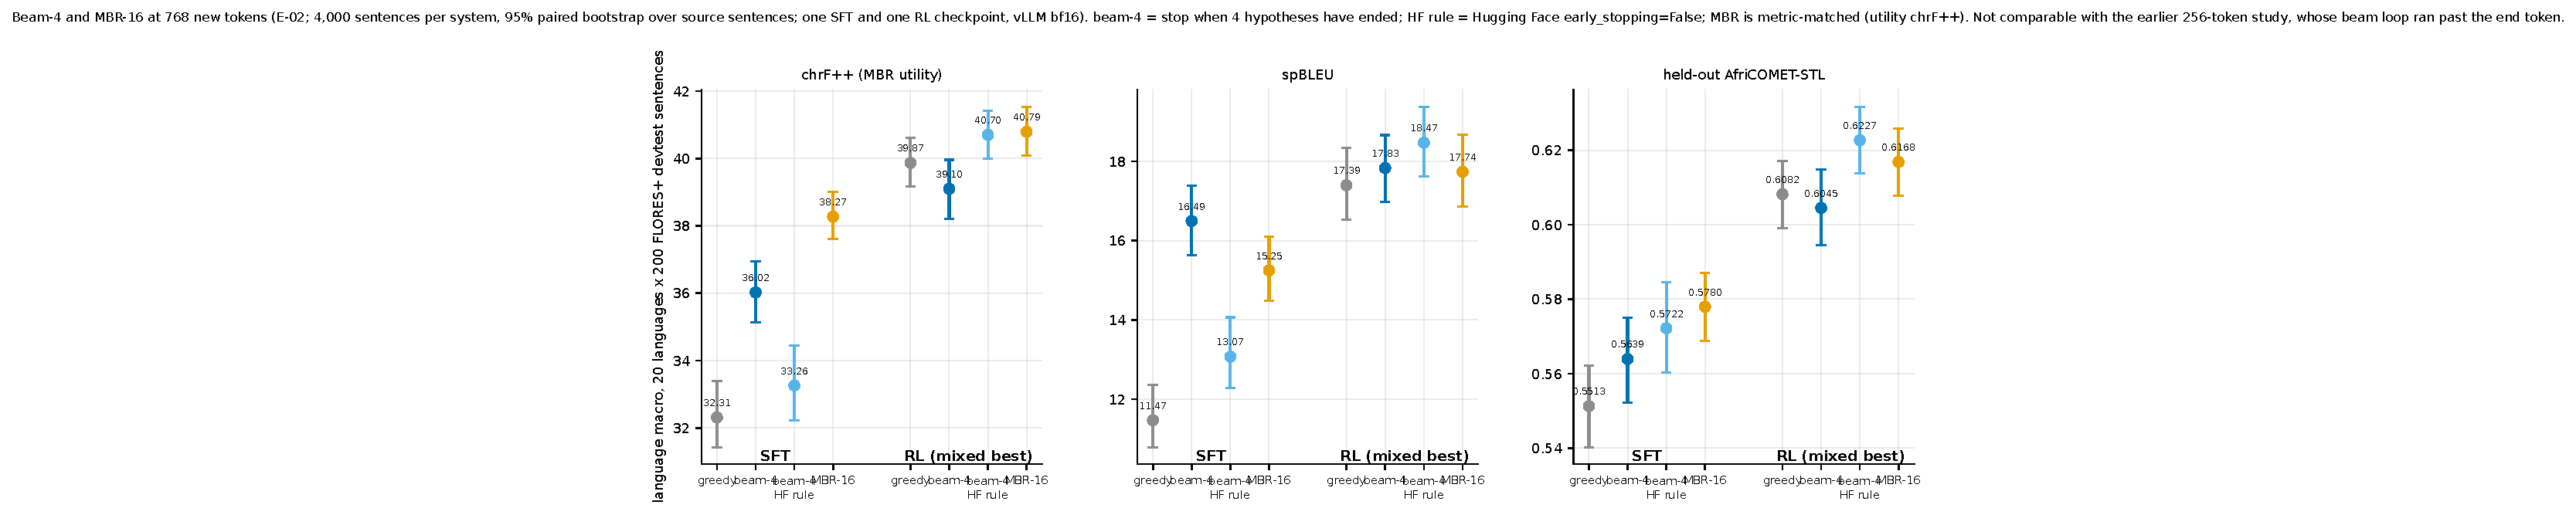
\includegraphics[width=1.00\linewidth,trim=384bp 0 384bp 26bp,clip]{figures/fig15_e02_decoding.pdf}
\caption{Greedy, beam-4 and MBR-16 at 768 new tokens (E-02) for the SFT and the RL model (mixed best): chrF++, spBLEU and held-out AfriCOMET-STL, language macro over 20 languages $\times$ 200 FLORES+ devtest sentences (4,000 per system), 95\% paired bootstrap over source sentences; beam-4 stops when 4 hypotheses have ended, the HF rule is early\_stopping=False, MBR is metric-matched (utility chrF++). One SFT and one RL checkpoint, vLLM bf16. Not comparable with the earlier 256-token study. Source: \texttt{reports/\allowbreak{}data/\allowbreak{}e02\_\allowbreak{}beam\_\allowbreak{}mbr\_\allowbreak{}768\_\allowbreak{}2026-\allowbreak{}11-\allowbreak{}05/\allowbreak{}cmp\_\allowbreak{}all.\allowbreak{}json}.}\label{fig:decoding_app}
\end{figure}

\begin{figure}[t]
\centering
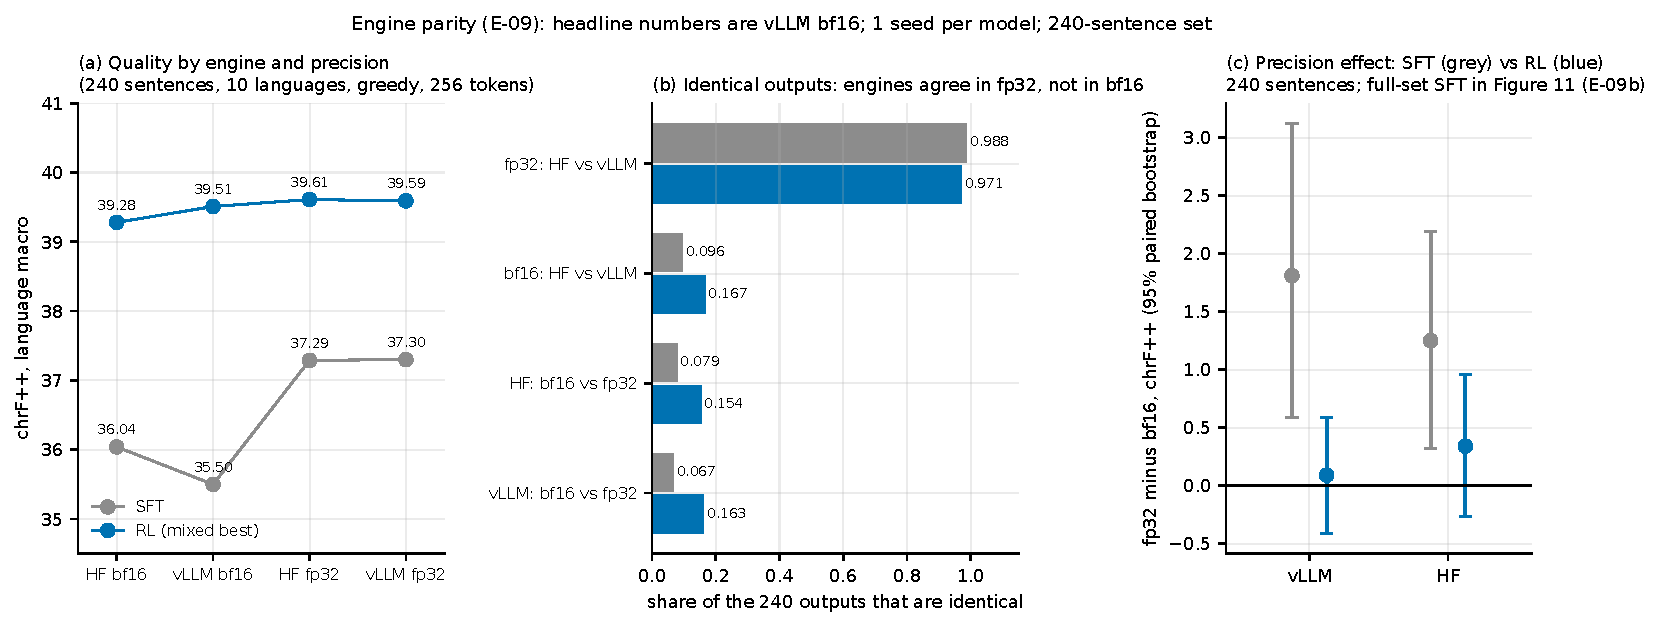
\includegraphics[width=1.00\linewidth]{figures/fig8_engine_parity.pdf}
\caption{Engine parity (E-09), 240 sentences (10 languages $\times$ 24 FLORES+ devtest sentences), greedy, 256 new tokens, SFT and RL (mixed best), one seed. (a) Language-macro chrF++ by engine and precision. (b) Share of identical outputs: vLLM and HF agree in fp32 (0.988, 0.971) and not in bf16 (0.096, 0.167). (c) fp32 minus bf16 chrF++ with 95\% paired bootstrap over sentences: negligible for the RL model, +1.81 [+0.59, +3.12] (vLLM) for the SFT on this small set, which the full-set run of Figure 11 does not reproduce. Headline numbers of the paper are vLLM bf16. Sources: \texttt{reports/\allowbreak{}data/\allowbreak{}e09\_\allowbreak{}engine\_\allowbreak{}parity\_\allowbreak{}2026-\allowbreak{}11-\allowbreak{}04/\allowbreak{}\{parity\_\allowbreak{}bootstrap,parity\_\allowbreak{}summary\}.\allowbreak{}json}.}\label{fig:fig8_engine_parity}
\end{figure}

\begin{figure}[t]
\centering
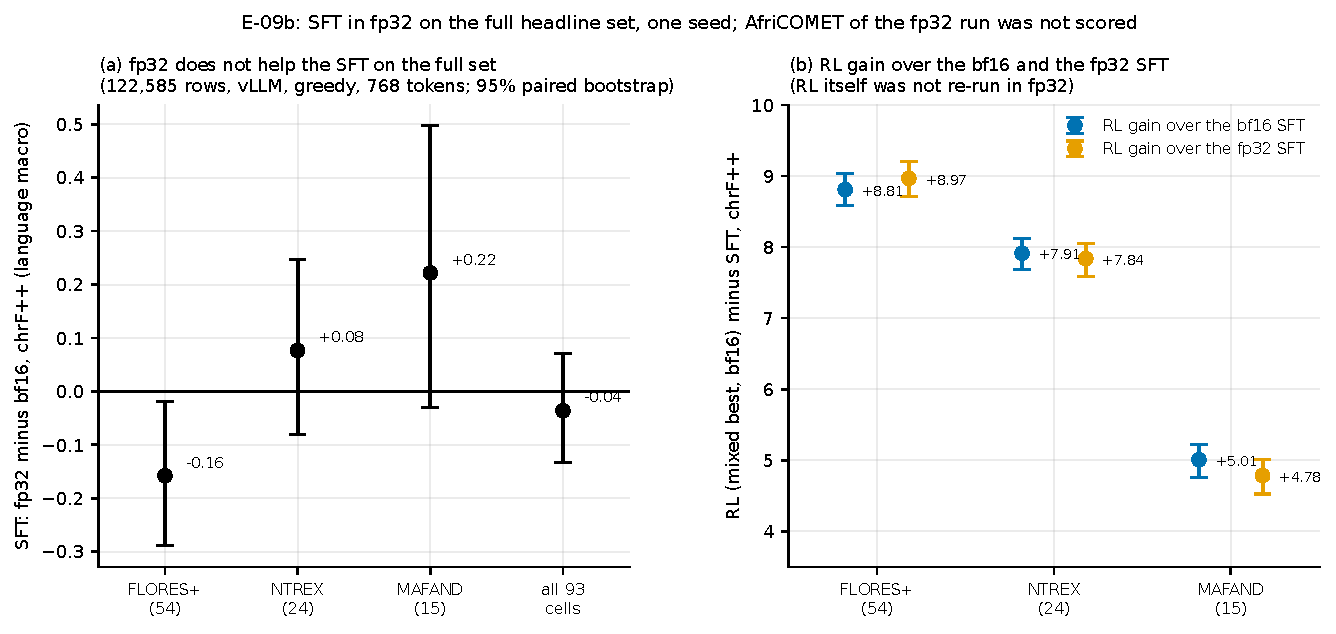
\includegraphics[width=0.90\linewidth]{figures/fig11_fp32_full_set.pdf}
\caption{Full-set precision check (E-09b): the SFT generated in fp32 instead of bf16 (vLLM, greedy, 768 new tokens, 122,585 rows, 214 flagged rows removed; one seed). (a) fp32 minus bf16 chrF++ (language macro, 95\% paired bootstrap over sentences) on FLORES+ (54 languages), NTREX (24), MAFAND (15) and over all 93 cells (\ensuremath{-}0.04 [\ensuremath{-}0.13, +0.07]). (b) RL gain (mixed best, bf16) over the bf16 SFT and over the fp32 SFT. The RL model was not re-run in fp32 and the AfriCOMET of the fp32 run was not scored. Source: \texttt{reports/\allowbreak{}data/\allowbreak{}e09b\_\allowbreak{}fp32\_\allowbreak{}2026-\allowbreak{}11-\allowbreak{}04/\allowbreak{}evidence\_\allowbreak{}e09b.\allowbreak{}json}.}\label{fig:fig11_fp32_full_set}
\end{figure}

\section{NLLB comparison and other systems: details}\label{app:afrique}

The RL closes 74\% of the gap between the SFT and NLLB-3.3B (12.50 $\to$ 3.26; arithmetic of the two differences), and stage A alone gives 8.61 of the 9.24 chrF++ that the mixed best adds over the SFT on these languages (93\%). The remaining gap is not a finishing or looping artefact: on these 43 languages the mixed best finishes at least 0.99 and repeats at most 0.02 in every language. By NLLB-3.3B tertile (14 / 14 / 15 languages) the mixed best reaches 91.7\% (high, 46.82 against 51.05), 87.7\% (mid, 34.57 against 39.42) and 96.8\% (tail, 25.92 against 26.78) of NLLB-3.3B; the SFT 75.3\%, 63.2\% and 60.7\%. The mixed best matches or beats NLLB-3.3B on 7 of 43 languages, all in the lowest tertile (yor +5.43, fon +2.95, dyu +2.77, wol +2.48, kam +2.32, kmb +2.22, umb +1.86; the SFT only on fon, 20.17 against 19.30) and is within 1 chrF++ on 9. The largest remaining gaps are amh \ensuremath{-}11.28, kin \ensuremath{-}9.74, kea \ensuremath{-}8.72, run \ensuremath{-}8.02, ewe \ensuremath{-}7.03, lug \ensuremath{-}6.77, tir \ensuremath{-}6.06 and hau \ensuremath{-}6.04. 
% src: NLLBRL sections 0, 2, 3 (`table3_by_nllb_tertile.csv`, `table2_per_language_43.csv`)

\textbf{Same sentences.} In the post-editor run, NLLB-3.3B and RL stage A drafts were scored on identical 100-sentence FLORES+ subsets (language bootstrap only; sentence hypotheses are not stored). With beam-4 on our side (the beam setup of the post-editor run, not that of E-02) and NLLB greedy on theirs, stage A is 1.44 below NLLB-3.3B on 43 languages (36.12 against 37.56, [\ensuremath{-}2.34, \ensuremath{-}0.56]; 13 languages at least equal) and 3.67 below on all 50 languages both have; held-out AfriCOMET 0.6414 against 0.6709 (\ensuremath{-}0.0294 [\ensuremath{-}0.0366, \ensuremath{-}0.0222], 40 languages, ahead in 5). Our own NLLB run on 100 sentences is 1.23 [\ensuremath{-}1.60, \ensuremath{-}0.86] below the published full-devtest value, which bounds the sample and reference effects. AfriCOMET is the QE reward's family, so that row is not independent evidence for the RL model. 
% src: NLLBRL section 4 (`table6b_same_sentence_summary.csv`, `table7_africomet_same_100_sentences.csv`)

\textbf{AfriqueLLM family, indicative only.} On the 21 languages with per-language values in the 5-shot AfroBench-Lite harness (afr amh ewe hau ibo kin lin lug nya orm sna som sot swh tir tsn twi wol xho yor zul): SFT 32.37, stage A 39.13, B1 best 39.32, mixed best 39.40, weak final 39.26, against AfriqueQwen3.5-4B-50Langs 41.71 (mixed best \ensuremath{-}2.31; ahead in 4 of 21 languages), AfriqueGemma-12B 38.58 (+0.83; 6 of 21), AfriqueLlama-8B 36.71, AfriqueQwen-14B 36.67, AfriqueQwen-8B 35.06, AfriqueGemma-4B 31.12, Gemma3-12B 18.82, Llama3.1-8B 16.45. Those are base models in 5-shot prompting with a harness whose chrF++ implementation and FLORES split are not verified.   Bidirectional aggregates (TranslatePsy, AfriNLLB) and pooled AfroBench rows are not comparable and are not compared.
% src: NLLBRL section 5 `table5_afrique_21_languages.csv`; ledger N3 status weak

\section{Family, script and resource level (exploratory, fragile)}\label{app:family}

We labelled all 125 registry languages with Glottolog 5.3 \citep{glottolog53} (CLDF release v5.3, commit 072ca0d of glottolog-cldf, CC BY 4.0, Zenodo 10.5281/zenodo.18840967) and asked whether the RL gain (mixed best minus SFT, FLORES+ devtest chrF++, 54 languages) depends on family, script or resource level. \textbf{This analysis is observational, has 54 languages in 7 families, several with 1 to 3 members, and its main result changes with the languages included. We report it as description, not as a finding.} 
% src: FAMILY sections 0, 3-5

\begin{table}[t]
\centering\scriptsize
\setlength{\tabcolsep}{4pt}
\caption{RL gain (mixed best minus SFT, FLORES+ devtest \chrfpp{}, 54 languages) by Glottolog family, script and regression family; bootstrap over languages.}\label{tab:family}
\begin{tabularx}{\linewidth}{@{}l>{\raggedright\arraybackslash}Xrr>{\raggedright\arraybackslash}X@{}}
\toprule
grouping & group & n & mean SFT chrF++ & mean gain [bootstrap CI over languages] \\
\midrule
Glottolog top family & Atlantic-Congo & 33 & 26.20 & +9.14 [+7.58, +10.79] \\
 & Afro-Asiatic & 11 & 13.45 & +6.89 [+4.29, +9.89] \\
 & Nilotic & 3 & 12.87 & +11.58 [+10.30, +13.13] \\
 & Indo-European (creoles, Afrikaans) & 3 & 36.85 & +10.23 [+1.01, +20.27] \\
 & Mande & 2 & 14.65 & +8.42 [+7.78, +9.06] \\
regression family & Narrow Bantu & 24 & 27.36 & +9.91 [+7.96, +11.71] \\
 & other Atlantic-Congo & 9 & 23.11 & +7.06 [+4.76, +9.61] \\
script & Latin & 48 & 24.84 & +9.32 [+8.03, +10.68] \\
 & Ethiopic (amh tir) & 2 & 13.55 & +9.13 [+8.26, +10.00] \\
 & Arabic (aeb ary arz) & 3 & 4.00 & +2.73 [+1.36, +4.59] \\
 & Tifinagh (zgh) & 1 & 2.29 & +1.78 \\
\bottomrule
\end{tabularx}
\end{table}

(Single-language groups, Saharan knc and Austronesian mlg, are in the report. Glottolog's Nilotic group differs from the earlier ``Nilo-Saharan'' group of EVID Table 4 by dik versus knc, which is why the two means agree, +11.58 and +11.62.)

\begin{itemize}
\item The lowest gains are the Arabic-script dialects and Tifinagh, the languages where the SFT's output was English, Arabic or loops and the RL did not repair it (Section~\ref{sec:rlsft}). The eight languages that lacked a family label are now labelled: aeb, ary and arz Afro-Asiatic (Semitic, Arabic script), taq and zgh Afro-Asiatic (Berber), cjk Narrow Bantu, dik Nilotic, mfe French-lexifier creole. 
% src: FAMILY section 2 (`unlabelled8_labels.csv`)
\item \textbf{The gain is not explained by the token budget} (Spearman rho(gain, log10 SFT tokens) = \ensuremath{-}0.16 [\ensuremath{-}0.44, +0.13], n = 54; OLS slope +0.34 chrF++ per log10 unit [\ensuremath{-}2.03, +1.79], R2 0.003), while the SFT level is (rho = +0.68 [+0.47, +0.82]; slope +11.8 [+8.5, +17.0], R2 0.45). \textbf{This is fragile:} dropping Afro-Asiatic turns the slope on the gain from +0.34 into \ensuremath{-}3.00 (SE 1.06), so ``no relation'' depends on which languages are in the sample. What the gain does track is the SFT's failure rate (rho with the SFT finished rate \ensuremath{-}0.47 [\ensuremath{-}0.74, \ensuremath{-}0.15], with its repeat rate +0.46 [+0.13, +0.72], n = 54 each), in line with Section~\ref{sec:rlsft}: family, script and resource effects on the raw gain are largely effects on how badly the SFT failed.
\item A regression of the gain on family, log tokens, non-Latin script, AfriCOMET availability and NLLB-mined share (n = 53, 11 parameters) explains little (R2 0.27, adjusted 0.09). Only non-Bantu against Narrow Bantu Atlantic-Congo is clearly non-zero (\ensuremath{-}4.45 [\ensuremath{-}8.36, \ensuremath{-}1.24], robust p = 0.020, uncorrected for the many contrasts); the NLLB-mined share is positive (+7.57 [+0.91, +14.67], p = 0.066), which reflects that NLLB-dependent languages are the low-resource tail that started low and failed by loops; it does not say whether NLLB data helped or hurt (Appendix~\ref{app:nllblink}). The same model explains most of the SFT level (R2 0.67, adjusted 0.59). Family, script, tokens, resource tier and AfriCOMET availability overlap (VIF 2.1 to 3.4), and three of six mixed-model fits did not converge.
\item Only 54 of 125 languages (58 with NTREX and MAFAND) have a gain; 51 have no reference test, so no family or script statement is possible for them. The 54 are the better-resourced languages (median 25.4 M tokens against 8.6 M for the Latin-script registry). The token table is provisional, the script of 51 languages is assigned from prior knowledge, and the analysis was run after the results were known.
\end{itemize}

\section{Science and document results: details}\label{app:docs}

Start: the mixed-stage best. Science SFT: AdamW 3e-6, 283 steps of 65,536 tokens (6.34 M AfriScience tokens in 6 languages, two passes, plus 12.19 M replay tokens), AfriScience dev loss 1.699 $\to$ 1.322. The SFT end point (alpha 1.0) loses 2.45 NTREX and 1.20 MAFAND chrF++, so the weights were interpolated, theta(alpha) = (1 - alpha) theta\_start + alpha theta\_science, with a rule fixed beforehand (best AfriScience dev chrF subject to NTREX and MAFAND not more than 0.5 below the start); alpha = 0.5 was chosen. 
% src: reports/eval_science_sft_385m_2026-11-04.md

\begin{table}[t]
\centering\footnotesize
\setlength{\tabcolsep}{4pt}
\caption{Weight interpolation sweep of the science SFT, AfriScience-MT test (macro over six languages), with NTREX and MAFAND-MT \chrfpp{} (last two columns). SSA-QE = SSA-COMET-QE (headline); AfriC. = AfriCOMET-STL.}\label{tab:alpha}
\begin{tabular}{@{}rrrrrrrrr@{}}
\toprule
$\alpha$ & SSA-QE & chrF & chrF++ & BLEU & spBLEU & AfriC. & NTREX & MAFAND \\
\midrule
0 & 0.6130 & 45.40 & 42.44 & 17.72 & 21.89 & 0.6828 & 37.16 & 40.78 \\
0.3 & 0.6128 & 46.28 & 43.40 & 18.73 & 23.25 & 0.6865 & 37.13 & 41.06 \\
0.5 (chosen) & 0.6118 & 46.63 & 43.80 & 19.27 & 23.87 & 0.6879 & 36.90 & 41.05 \\
0.7 & 0.6092 & 46.56 & 43.81 & 18.98 & 23.83 & 0.6859 & 36.43 & 40.83 \\
1.0 & 0.5986 & 44.92 & 42.30 & 16.78 & 20.87 & 0.6708 & 34.71 & 39.58 \\
\bottomrule
\end{tabular}
\end{table}

\textbf{The science SFT gives surface gains (chrF +1.2, BLEU +1.5, spBLEU +2.0 at alpha 0.5) and no SSA-COMET-QE gain} (dev 0.6242 against 0.6235). SSA-COMET-QE here is the reference-free \texttt{McGill-\allowbreak{}NLP/\allowbreak{}ssa-\allowbreak{}comet-\allowbreak{}qe}, the variant that reproduces the AfriScience-MT paper's released values (mean absolute difference 0.006 over the six strongest released runs, 0.031 over nine); there is no RL in this comparison, so it is independent of the reward.  The metric choice was made after the alpha rule (Appendix~\ref{app:disc}). The 385M with the science SFT is below the old 270M science-stage models on AfriScience test chrF (46.6 against 47.9 for the old RL-final, 50.0 and 50.2 for the old science-stage models) and below the published fine-tuned NLLB-1.3B (52.3). 
% src: SCI alpha sweep; DOC calibration; HYG X13 (SCI's caveat paragraph is stale, quote DOC)
% src: SCI Table 2

\textbf{Science RL.} The run executed 160 steps (cap extended from 150 to 190 at step 120, stopped on a dev plateau at step 150 plus a 10-step wind-down; Appendix~\ref{app:chain}, ledger X24). Evaluation was fixed in advance: independent evidence = plain chrF on AfriScience-MT test and held-out AfriCOMET; SSA-COMET-QE and SSA-COMET-MTL are reward-family and shown but not counted. The final checkpoint is a small real sentence-level gain over its start (science SFT, alpha 0.5): chrF +0.46 [+0.27, +0.65] on AfriScience test and held-out AfriCOMET +0.0053 [+0.0036, +0.0071]; the step-75 \texttt{best} checkpoint is smaller (chrF +0.16 [\ensuremath{-}0.04, +0.37]); SSA-COMET-QE moves by +0.004 only; NTREX and MAFAND do not regress (chrF++ +0.42, +0.10). There is no document-level gain: chunked window SSA-COMET-QE is 0.574 (start), 0.574 (best), 0.577 (final), and the earlier 270M work's 270M models stay ahead on sentence chrF (47.9-50.2 stored numbers against 47.10) and on chunked documents (0.593 against 0.577). One run, one seed. Numbers: \texttt{reports/\allowbreak{}eval\_\allowbreak{}science\_\allowbreak{}rl\_\allowbreak{}385m\_\allowbreak{}2026-\allowbreak{}11-\allowbreak{}04.\allowbreak{}md}. \textbf{Disclosure:} the long-document RL start model was changed from \texttt{best} to \texttt{final} after this evaluation, including its test numbers (rule refined on the full AfriScience dev set, where final beats best by +0.24 chrF and +0.0031 AfriCOMET; the test split was not used for the rule); logged in \texttt{reports/\allowbreak{}overnight\_\allowbreak{}log\_\allowbreak{}2026-\allowbreak{}11-\allowbreak{}04.\allowbreak{}md}. SSA-COMET-QE, AfriCOMET and chrF for every stage are tabulated below (E-05). The RL-only science arm (mixed best to science RL without the science SFT) is reported next (E-14).

\textbf{Science RL without the science SFT (E-14).} To ask whether the science SFT is needed, the executed science RL was repeated with the start model changed to the mixed best (= science-SFT alpha 0, the model the science SFT was built from): same seed 1234, same pool, same reward, Muon at 1e-6, KL 0.1 against the start model, 160 steps (150 plus a 10-step wind-down), pre-declared checkpoint = final. The rule was registered before the run: the science SFT is \emph{not needed} if the lower 95\% bounds of E-14 minus the science RL final on AfriScience-MT test are above \ensuremath{-}0.5 chrF and above \ensuremath{-}0.004 held-out AfriCOMET; it is \emph{needed} if the upper bound of either is below its margin. 

\begin{table}[t]
\centering\footnotesize
\setlength{\tabcolsep}{4pt}
\caption{Science RL without the science SFT (E-14): AfriScience-MT test, sentence level, macro over 6 languages.}\label{tab:e14a}
\begin{tabularx}{\linewidth}{@{}>{\raggedright\arraybackslash}Xrrrr@{}}
\toprule
model & chrF & chrF++ & AfriCOMET-STL (held out) & SSA-COMET-QE (reward family) \\
\midrule
mixed best (= alpha 0; E-14's start) & 45.40 & 42.44 & 0.6828 & 0.6130 \\
B1 final (stage-B1 RL) & 45.45 & 42.50 & 0.6846 & 0.6141 \\
\textbf{E-14 final (science RL, no science SFT)} & \textbf{45.66} & 42.69 & \textbf{0.6850} & 0.6153 \\
science SFT alpha 0.5 & 46.63 & 43.80 & 0.6879 & 0.6118 \\
science RL final (from the science SFT) & 47.10 & 44.22 & 0.6932 & 0.6158 \\
\bottomrule
\end{tabularx}
\end{table}

\begin{table}[t]
\centering\footnotesize
\setlength{\tabcolsep}{4pt}
\caption{E-14 final minus X, 95\% bootstrap (independent weights per language).}\label{tab:e14b}
\begin{tabularx}{\linewidth}{@{}>{\raggedright\arraybackslash}Xll>{\raggedright\arraybackslash}X@{}}
\toprule
E-14 final minus & chrF & AfriCOMET-STL (held out) & SSA-COMET-QE (reward family) \\
\midrule
science RL final (from the science SFT) & \textbf{-1.44 [\ensuremath{-}1.61, \ensuremath{-}1.25]} & \textbf{-0.0082 [\ensuremath{-}0.0101, \ensuremath{-}0.0065]} & \ensuremath{-}0.0006 [\ensuremath{-}0.0018, +0.0007] \\
science SFT alpha 0.5 & \ensuremath{-}0.97 [\ensuremath{-}1.20, \ensuremath{-}0.75] & \ensuremath{-}0.0030 [\ensuremath{-}0.0050, \ensuremath{-}0.0009] & +0.0035 [+0.0022, +0.0047] \\
mixed best (its own start) & +0.26 [+0.12, +0.39] & +0.0022 [+0.0007, +0.0036] & +0.0023 [+0.0013, +0.0033] \\
B1 final & +0.21 [+0.07, +0.36] & +0.0004 [\ensuremath{-}0.0012, +0.0020] & +0.0012 [+0.0000, +0.0023] \\
\bottomrule
\end{tabularx}
\end{table}

\textbf{By the registered rule the science SFT is needed:} the upper bounds are \ensuremath{-}1.25 chrF and \ensuremath{-}0.0065 AfriCOMET, both below their margins, chrF is lower in all six languages (\ensuremath{-}0.72 to \ensuremath{-}2.70) and the dev split agrees (\ensuremath{-}1.63 [\ensuremath{-}1.81, \ensuremath{-}1.44]). The science gain is carried by the science SFT (+1.23 chrF at alpha 0.5), not by the science RL: the RL alone on top of the mixed best adds +0.26 chrF [+0.12, +0.39] (+0.0022 AfriCOMET), a gain of the size at which seed noise matters (E-04), against +0.46 for the RL on top of the science SFT. The trainer's dev chrF++ stayed flat (43.50 $\to$ 43.43) while the executed science RL rose from 44.62 to 45.13, and no \texttt{best/\allowbreak{}} checkpoint was written (the dev macro never rose by the trainer's 0.2 margin), so only the final exists. \textbf{Reward-family caveat:} SSA-COMET-QE rates E-14 level with the science RL final (\ensuremath{-}0.0006 [\ensuremath{-}0.0018, +0.0007]) and above alpha 0.5 (+0.0035), while chrF and held-out AfriCOMET rate it below both: the metric the RL optimises moved without a matching move in the independent metrics, so it is not evidence of quality here. On the general benchmarks (93 cells) E-14 is +0.13 chrF++ [+0.10, +0.15] over the mixed best (FLORES+ +0.17, NTREX +0.12, MAFAND 0.00) and +0.34 [+0.31, +0.36] over B1 final, with no regression on NTREX and MAFAND (+0.12 / 0.00 against the mixed best; the executed science RL final is higher on MAFAND by 0.36); at document level it does not change chunked chrF (57.30 against 57.29 for its start) and whole-document decoding still fails (finished 0.69, loop 0.82, chrF 25.6). Caveats: one seed; one crash (a CUDA out-of-memory in the COMET reward worker at about step 38; the launcher's ladder halved the micro-batch from 12,288 to 6,144 tokens and resumed from the step-20 checkpoint, replaying steps 21 to 38, which can differ from the first pass because vLLM sampling is not bit-reproducible); the comparison with the science RL final mixes the effect of the science SFT with its alpha 0.5 interpolation (a science SFT at alpha 1.0 followed by RL was not run); 160 steps only. 
% src: reports/e14_science_rl_without_science_sft_2026-11-05.md sections 0-3; reports/data/e14_science_rl_no_sft_2026-11-05/ (ledger E14 rows SC7, SC8)

\textbf{SSA-COMET-QE for every stage (E-05).} The stored AfriScience-MT sentence predictions of every stage were scored with \texttt{McGill-\allowbreak{}NLP/\allowbreak{}ssa-\allowbreak{}comet-\allowbreak{}qe}, held-out AfriCOMET-STL and plain chrF (test, macro over 6 languages). SSA-COMET-QE is 0.5686 for the SFT and 0.6118 (stage A), 0.6113 (B1 best), 0.6130 (mixed best), 0.6118 (science SFT alpha 0.5), 0.6135 / 0.6158 (science RL best / final) and 0.6158 / 0.6165 (long-document RL best / final) for the RL stages: the first RL stage adds +0.043 and every later stage at most +0.005 more. It is a reward-family metric for every RL row, so these numbers are not evidence of quality; chrF (36.00 for the SFT, 45.06 stage A, 45.40 mixed, 46.63 science SFT, 47.10 science RL final, 47.16 long-document RL) and held-out AfriCOMET-STL (0.6064, 0.6822, 0.6828, 0.6879, 0.6932, 0.6936) keep rising by small steps that SSA-COMET-QE does not register. Alpha 1.0 (the full science SFT) is the only row clearly worse (0.5986). One seed per stage; test-sentence bootstrap intervals of the differences are +/\ensuremath{-}0.001 to +/\ensuremath{-}0.002 (Section~\ref{sec:science} tables). The numbers are for sentence level and are not comparable with the AfriScience-MT paper's document-level table. 
% src: reports/e05_ssa_all_stages_2026-11-04.md; reports/data/e05_ssa_all_stages_2026-11-04/{tables.md,e05_all.json} (ledger SC6, P4)

168 test documents (28 papers $\times$ 6 languages), a document being the paper's plain-language summary rebuilt from sentences. Whole-document generation (greedy, 4,096 new tokens) fails for the 385M models and is worse after the science SFT: start finished 0.71, loop 0.86, chrF 22.8, tail coverage 0.27; science SFT finished 0.51, loop 0.86, chrF 24.9; the old 270M RL-final finished 0.70, loop 0.61, chrF 34.9. Sentence-by-sentence (``chunked'') decoding with best-of-4 repair fixes finishing for all three (finished 1.00, sentence coverage 1.000): 
% src: reports/eval_afriscience_document_level_2026-11-04.md Tables 1-3

\begin{table}[t]
\centering\footnotesize
\setlength{\tabcolsep}{4pt}
\caption{Chunked document decoding (sentence by sentence with best-of-4 repair), 168 test documents.}\label{tab:docs}
\begin{tabularx}{\linewidth}{@{}>{\raggedright\arraybackslash}Xrrrr@{}}
\toprule
model (chunked) & SSA-COMET-QE, 4-sentence windows & chrF & AfriCOMET window & BLEU \\
\midrule
385M start (alpha 0) & 0.574 & 57.3 & 0.687 & 20.0 \\
385M science SFT (alpha 0.5) & 0.574 & 58.8 & 0.692 & 22.0 \\
old 270M RL-final (earlier 270M work) & 0.593 & 59.3 & 0.703 & 22.5 \\
\bottomrule
\end{tabularx}
\end{table}

The earlier 270M work's 270M RL-final is as good as or better than the 385M at document level (+0.019 window SSA-COMET-QE, +0.011 AfriCOMET window, +0.5 to +2.0 chrF; better on hau, lug, nso, zul, worse on amh). The COMET encoders read 512 tokens, so a concatenated-document COMET only sees the start of a document; the window values are the honest ones. Window SSA-COMET-QE is reward-family for the old model (trained against a QE reward); chrF and AfriCOMET are the independent checks. For reference, the AfriScience-MT paper's best released document-level system (GPT-5.4) has SSA-COMET 0.519 and chrF 64.5 under document handling we cannot reproduce. Caveats: one seed, 28 papers per language, no bootstrap. None of the 385M RL stages trained on prompts above 256 source tokens before the long-document RL; production use is sentence by sentence.

\textbf{Long-document RL.} The stage started from the science RL final (step 160), ran the planned 80 steps (32 prompts per step, about 51\% long prompts of 512 to 2,048 source tokens, group 8, no guide, hold-out-reward checkpoint selection, LibreTexts-free pool) and was evaluated at its best (step 50) and final (step 80) checkpoints on the same 168 documents. In whole-document mode, best against its start: finished \textbf{0.70 $\to$ 0.82 (+0.125 [+0.046, +0.204])}, loop rate \textbf{0.85 $\to$ 0.73 (\ensuremath{-}0.113 [\ensuremath{-}0.179, \ensuremath{-}0.056])}, chrF \textbf{27.4 $\to$ 30.9 (+3.4 [+1.5, +5.3])}, tail coverage 0.32 $\to$ 0.36 (95\% bootstrap over documents). The final checkpoint is similar (finished 0.85, loop 0.72, chrF 29.7, +2.2 [+0.4, +4.2], length ratio 0.81); best and final do not differ significantly (chrF \ensuremath{-}1.2 [\ensuremath{-}3.0, +0.7]). \textbf{Whole-document decoding remains unusable:} 15 to 18\% of the documents do not finish, 72 to 73\% show a repetition loop, and the output covers 34 to 36\% of the last third of the paper (chunked: 63\%). Chunked and sentence-level results do not change: window SSA-COMET-QE (reward family) 0.577 $\to$ 0.579 and 0.579 (a corpus-level number, no interval; a 0.002 difference is not an effect), chunked chrF 58.7 $\to$ 58.9 / 58.8 (best +0.13 [+0.04, +0.22]); AfriScience test sentences chrF 47.10 $\to$ 47.16 (+0.06 [\ensuremath{-}0.09, +0.20]), held-out AfriCOMET +0.0001 / +0.0004 with intervals around zero; NTREX / MAFAND chrF++ 37.33 / 41.14 $\to$ 37.43 / 41.15 (best). The earlier 270M work's 270M RL-final is still ahead in chunked mode (window SSA-COMET-QE 0.593 against 0.579) and in whole-document chrF (34.9 against 30.9). The effect is real but moderate and of the size of the other late-stage steps; the hold-out loop rate fell by only 2 points over the 80 steps, and the selection reward is the optimised quantity. One seed; 168 documents from 28 papers, so the intervals reflect paper sampling only. 
% src: reports/eval_long_document_rl_385m_2026-11-04.md sections 0-3 (LDOLR); reports/data/eval_long_rl_2026-11-04/{doc_tables.md,doc_pairs.json,sci_pairs_long.json}; ledger DL5, P2. The report says "best/ vs final/ indistinguishable"; wall-clock and crash loop in Section 15

\subsection{Figures for the science and document results}\label{app:figs}

\begin{figure}[t]
\centering
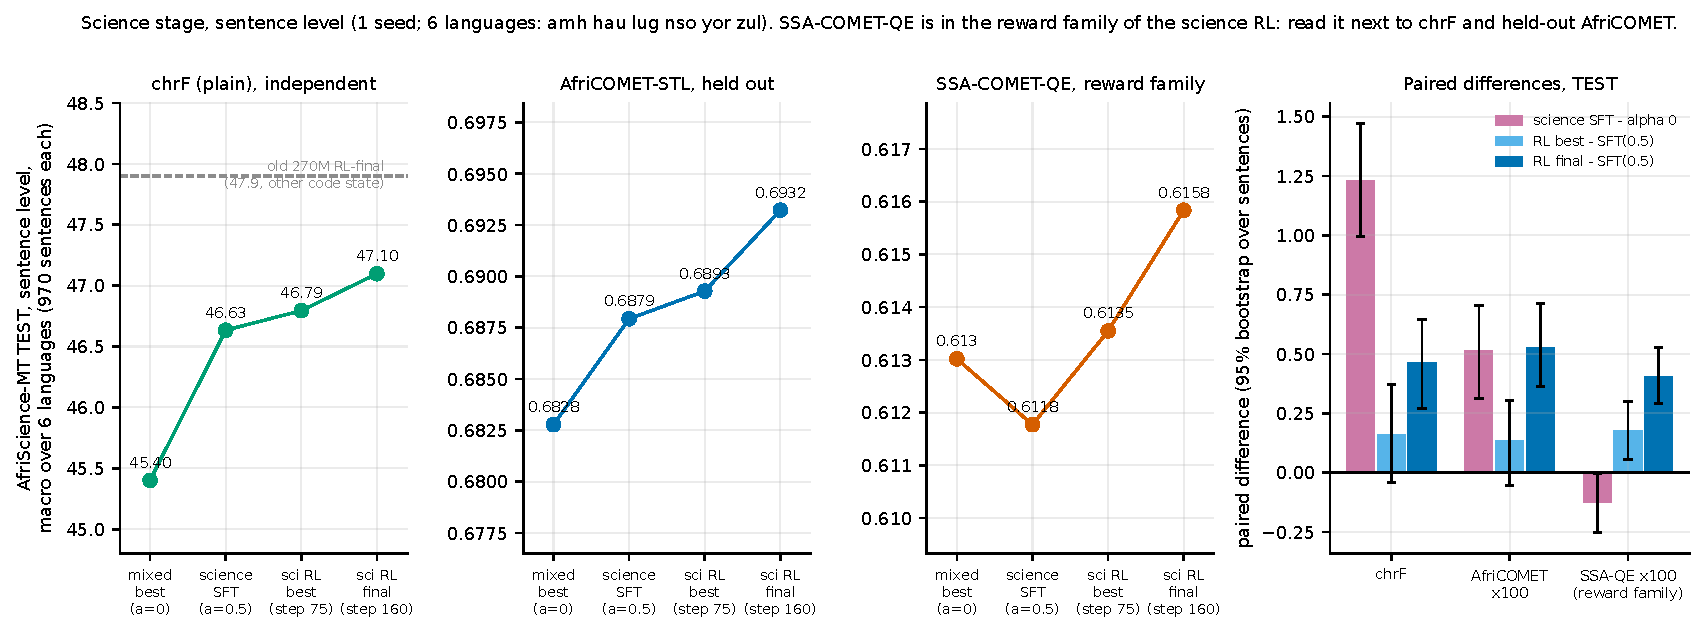
\includegraphics[width=1.00\linewidth]{figures/fig5a_science_sentence.pdf}
\caption{Science stage, AfriScience-MT TEST, sentence level (970 sentences per language, macro over amh hau lug nso yor zul; greedy; one seed): plain chrF (independent of the reward; dashed: the earlier 270M work's 270M RL-final, other code state), held-out AfriCOMET-STL (independent), and SSA-COMET-QE (reward family of the science RL) for the mixed best (alpha 0), the science SFT (alpha 0.5), and the science RL best (step 75) and final (step 160); right: paired differences with 95\% bootstrap over sentences. Sources: \texttt{reports/\allowbreak{}data/\allowbreak{}eval\_\allowbreak{}science\_\allowbreak{}rl\_\allowbreak{}2026-\allowbreak{}11-\allowbreak{}04/\allowbreak{}sci\_\allowbreak{}pairs.\allowbreak{}json}, \texttt{reports/\allowbreak{}data/\allowbreak{}eval\_\allowbreak{}science\_\allowbreak{}sft\_\allowbreak{}2026-\allowbreak{}11-\allowbreak{}04/\allowbreak{}tables.\allowbreak{}md}.}\label{fig:fig5a_science_sentence}
\end{figure}

\begin{figure}[t]
\centering
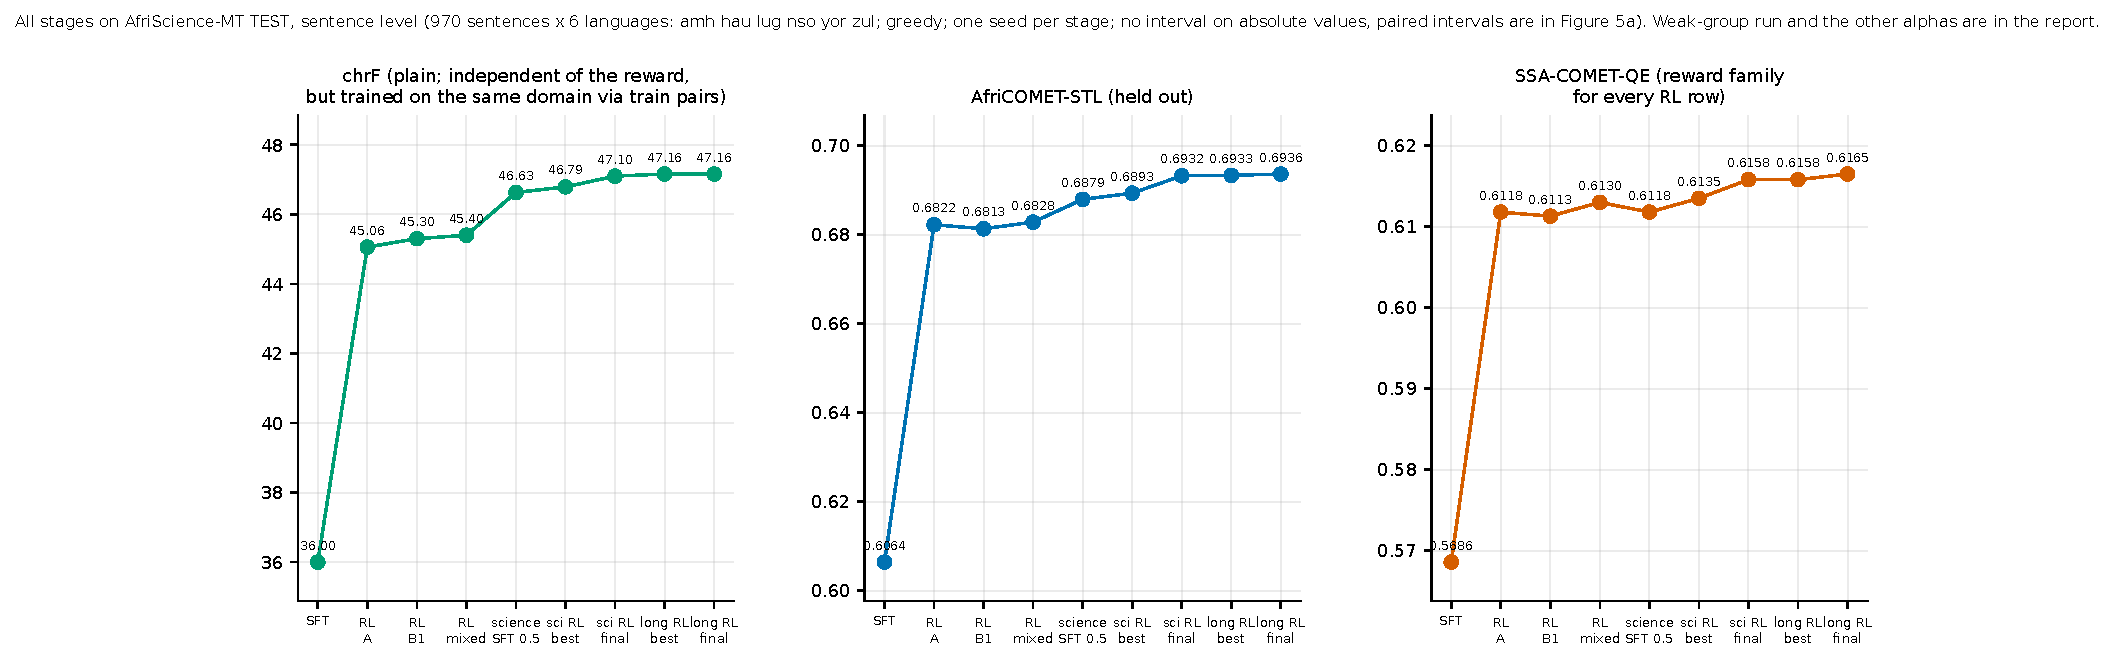
\includegraphics[width=1.00\linewidth]{figures/fig12_ssa_all_stages.pdf}
\caption{All stages on AfriScience-MT TEST, sentence level (970 sentences per language, macro over amh hau lug nso yor zul; greedy; one seed per stage): plain chrF, held-out AfriCOMET-STL and SSA-COMET-QE (reward family for every RL row) for the SFT, RL stages A, B1 and mixed, the science SFT (alpha 0.5), the science RL and the long-document RL. The weak-group run and the other interpolation weights are in the source table. Source: \texttt{reports/\allowbreak{}data/\allowbreak{}e05\_\allowbreak{}ssa\_\allowbreak{}all\_\allowbreak{}stages\_\allowbreak{}2026-\allowbreak{}11-\allowbreak{}04/\allowbreak{}tables.\allowbreak{}md}.}\label{fig:fig12_ssa_all_stages}
\end{figure}

\begin{figure}[t]
\centering
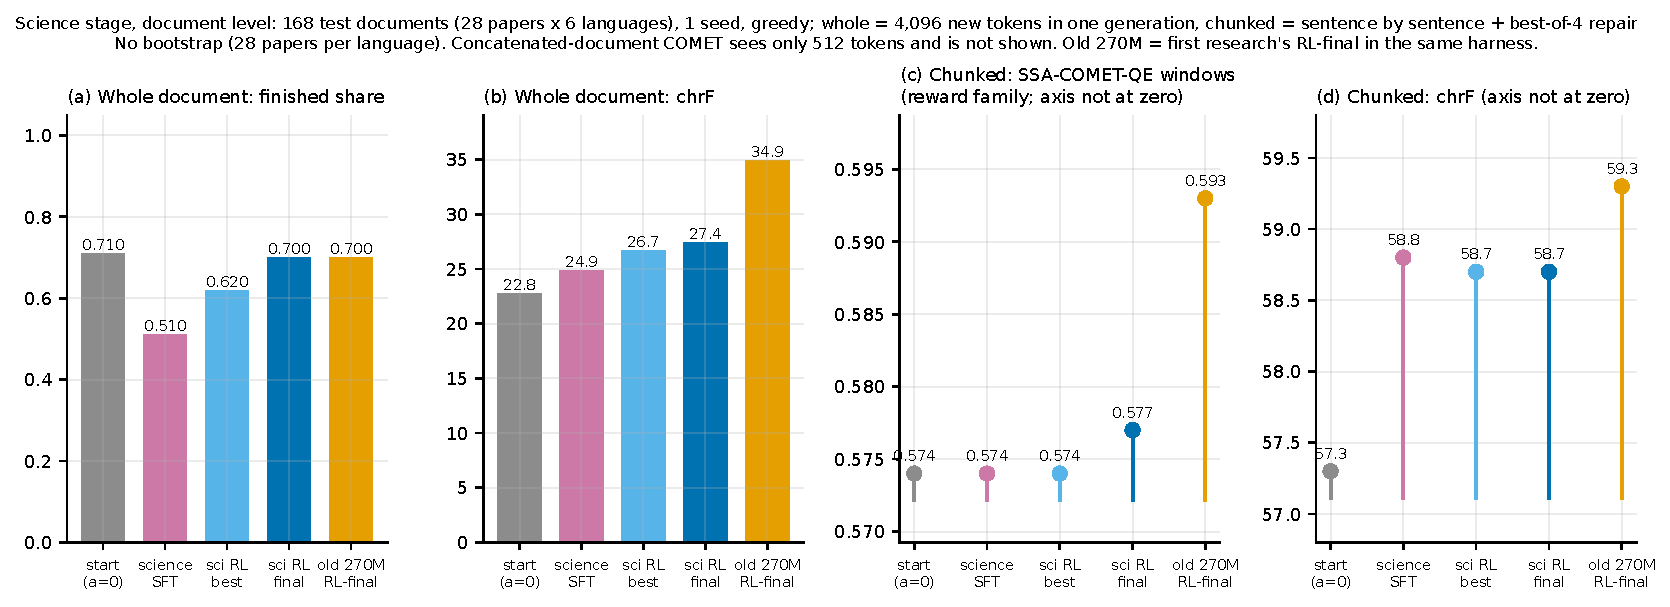
\includegraphics[width=1.00\linewidth]{figures/fig5b_science_document.pdf}
\caption{Science stage, document level: 168 test documents (28 papers $\times$ 6 languages), greedy, one seed, no bootstrap. Whole-document generation (4,096 new tokens): finished share and chrF. Chunked decoding (sentence by sentence plus best-of-4 repair): SSA-COMET-QE on 4-sentence windows (reward family) and chrF; axes of (c) and (d) do not start at zero. Source: \texttt{reports/\allowbreak{}data/\allowbreak{}eval\_\allowbreak{}science\_\allowbreak{}rl\_\allowbreak{}2026-\allowbreak{}11-\allowbreak{}04/\allowbreak{}doc\_\allowbreak{}tables.\allowbreak{}md}.}\label{fig:fig5b_science_document}
\end{figure}

\begin{figure}[t]
\centering
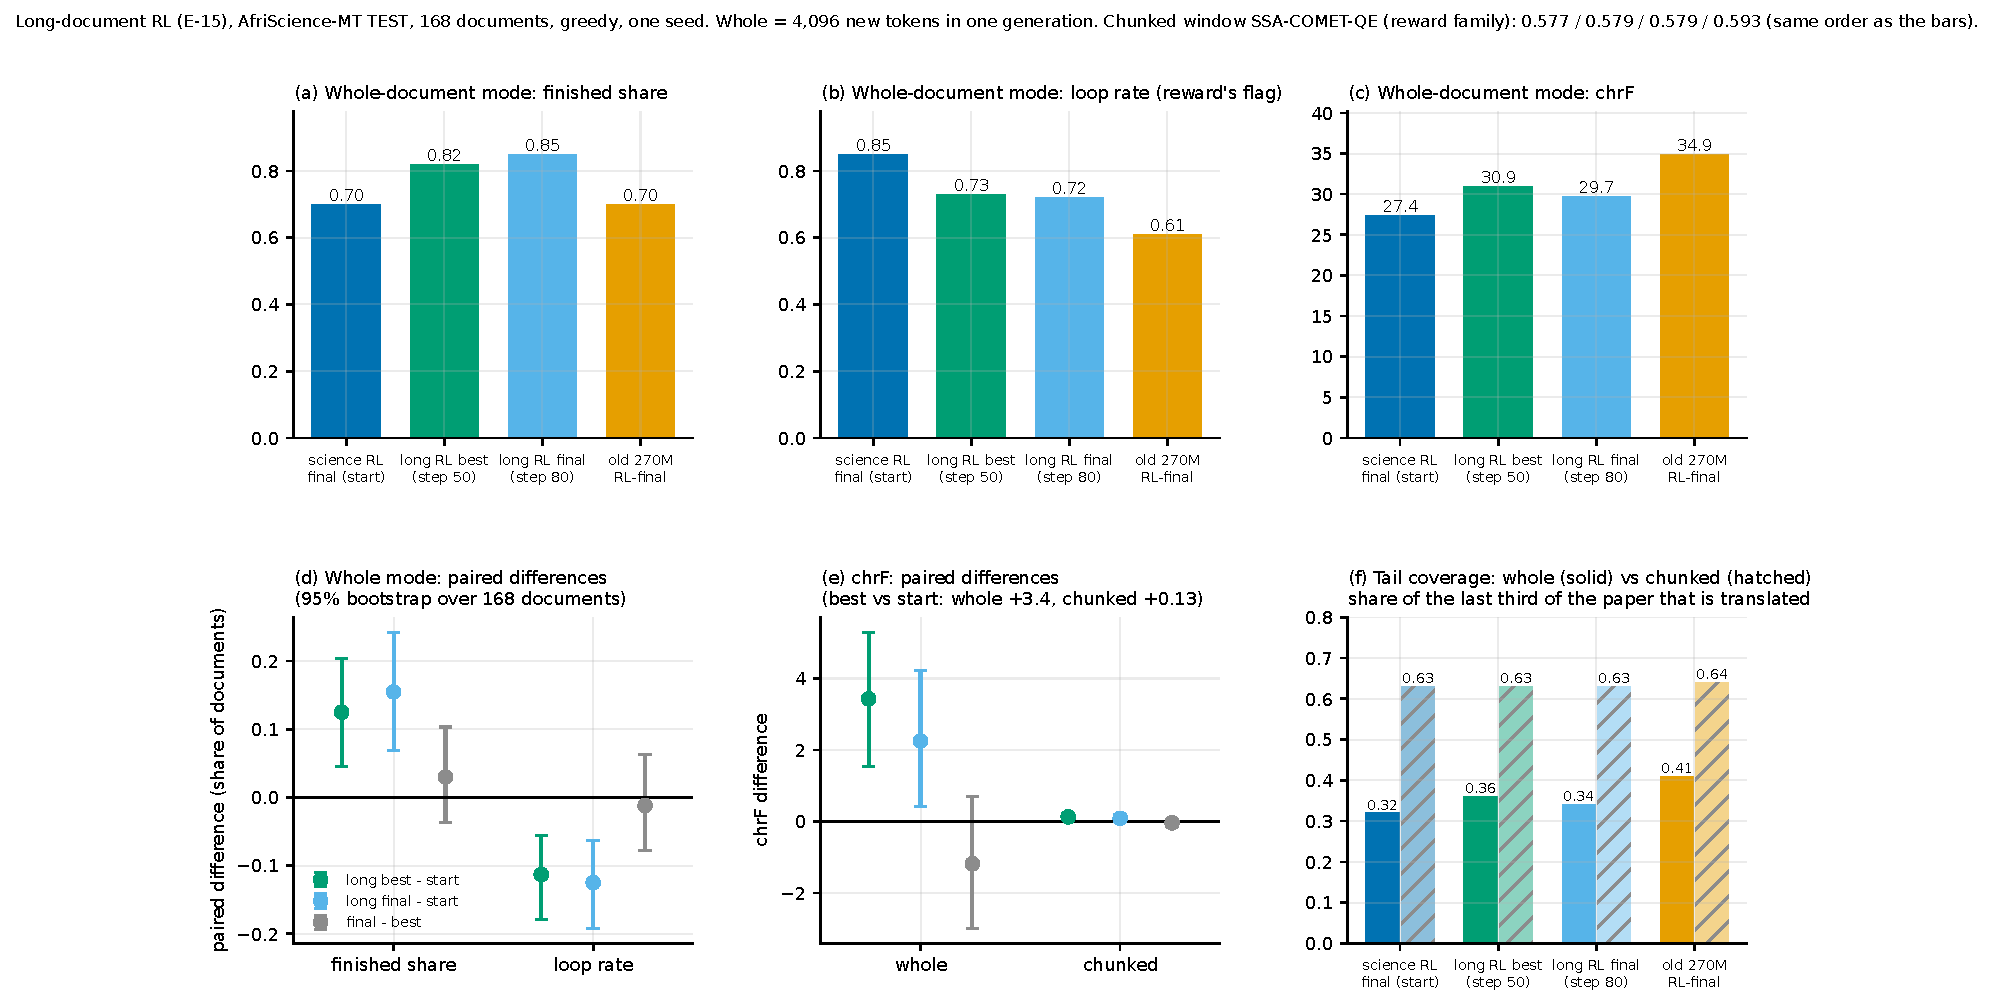
\includegraphics[width=1.00\linewidth]{figures/fig9_long_document_rl.pdf}
\caption{Long-document RL (E-15), AfriScience-MT TEST, 168 documents (28 papers $\times$ 6 languages), greedy, one seed. (a-c) Whole-document mode (4,096 new tokens in one generation): finished share, loop rate (the reward's flag) and chrF for the science RL final (the start), the long-document RL best (step 50) and final (step 80), and the earlier 270M work's 270M RL-final. (d, e) Paired differences with 95\% bootstrap over documents (Poisson weights): finished share, loop rate and chrF in whole mode, chrF in chunked mode. (f) Tail coverage, the share of the last third of the paper that is translated, whole against chunked mode. Chunked window SSA-COMET-QE (reward family) is in the figure title. Sources: \texttt{reports/\allowbreak{}data/\allowbreak{}eval\_\allowbreak{}long\_\allowbreak{}rl\_\allowbreak{}2026-\allowbreak{}11-\allowbreak{}04/\allowbreak{}\{doc\_\allowbreak{}tables.\allowbreak{}md,doc\_\allowbreak{}pairs.\allowbreak{}json\}}.}\label{fig:fig9_long_document_rl}
\end{figure}

\section{Contamination audit and follow-ups}\label{app:contam}

\textbf{6.4 Contamination.} The audit scanned both sides of 25,911,095 training samples (A0 packs and the six stage-B shards) against all benchmark rows: \textbf{no benchmark sentence of 3 or more words is in the training text}; FLORES+ devtest 0 of 54,648 rows, NTREX 120 of 47,928 (0.25\%), MAFAND 94 of 20,009 (0.47\%), SmolSent 45 of 38,833, GlotStoryBook 15 of 3,426, all one- or two-word strings; the FLORES+ dev train half is found in 23,706 of 23,760 rows (positive control); \texttt{all}, \texttt{clean}, \texttt{no\_\allowbreak{}pair} and \texttt{clean\_\allowbreak{}strict} macros agree within 0.01 chrF++. 
% src: reports/contamination_audit_385m_2026-11-03.md sections 1, 3, 6; reports/eval_385m_results_2026-11-03.md section 0

\emph{Follow-ups (CPU, 2026-11-04).} 
% src: CFU sections 0-6

\begin{itemize}
\item \textbf{Phrase level.} A lexical fuzzy scan of 56,975,939 pair rows and 4,277,612 instruction rows (reachable pair and instruction files, before gating and packing) finds no benchmark string of 8 or more tokens as a contiguous run. Strings of 4 to 7 tokens do occur inside longer training text (English side: MAFAND 134 of 17,428 strings, GlotStoryBook 30 of 898, NTREX 18 of 1,973, SALT 12 of 498; FLORES+ devtest, SmolSent, IbomMT and FLORES-MOZ 0); the audit's run rule and the intake filter test such short strings only for whole-sentence equality, so ``no benchmark sentence of 3 or more words'' holds for whole sentences, not for phrases. 263 (string, benchmark) cases of 8+ token English strings have a character-5-gram Jaccard $\ge$ 0.5 with some training text (MAFAND 184, SALT 27, NTREX 19, GlotStoryBook 15, SmolSent 6, FLORES+ devtest 4 of 1,012). These are candidates, not proof of leakage; their effect on scores was not measured.
\item \textbf{Prompts of the RL.} Stage A drew 6 flagged prompts of 28,120 (0.021\%); 6 of 1,345 prompts drawn for the seven languages whose prompt files had not been filtered (0.45\%), all distinct, in steps 72-364, source side only (this replaces the earlier estimate of about 0.15\%). The pool of the long-document RL (241,679 rows) has 0 rows flagged by the protected index.
\item \textbf{AfriScience-MT train versus the SFT text.} 305 of 34,007 train rows (0.9\%; hau 64, yor 116, zul 125) have their African-language sentence verbatim in the A0 pair data, all from \texttt{HuggingFaceFW/\allowbreak{}finetranslations}; 3 rows (yor 2, zul 1) as a pair. The packed shards were not scanned. The test papers are untouched (0 of 5,820 rows).
\item \textbf{A0 text.} The files support that A0's pack set is the first 138,873 packs of the audited g0 (identical per-language pack counts for 84 languages); pack content was not hash-compared.
\item \textbf{Not covered:} embedding or MT-round-trip paraphrase contamination, Gemma-3 pretraining, packed-shard coverage of the AfriScience train overlap and of the phrase scan (not run: these scans need the data box; Appendix~\ref{app:limits} item 15).
\end{itemize}

Benchmarks were evaluated many times; checkpoint choice used only the dev set (Appendix~\ref{app:limits}).

\section{NLLB-mined data and the regression against the earlier 270M work}\label{app:nllblink}

All 17 languages more than 5 chrF++ below the old SFT were already below with A0 (no NLLB-mined rows); the mean gap old SFT to A0 is \ensuremath{-}10.7 and A0 to 385M SFT +2.1; Venda (no NLLB rows) regressed \ensuremath{-}9.7. Spearman of NLLB share with the regression: \ensuremath{-}0.45 [\ensuremath{-}0.73, \ensuremath{-}0.09] on NTREX+MAFAND clean (n = 28), \ensuremath{-}0.07 [\ensuremath{-}0.35, +0.20] on the pooled index (n = 57), \ensuremath{-}0.17 [\ensuremath{-}0.54, +0.23] after RL. Each factor of 10 in NLLB-mined tokens adds \ensuremath{-}0.4 chrF++ (bootstrap 95\% [\ensuremath{-}11.0, +4.8]) against +9.6 for other new tokens. NLLB-mined rows are noisier than the same language's other rows (GlotLID acceptance median 0.77 against 0.99; AfriCOMET-QE below the language median in 38 of 43 languages). The decisive ablation (about 34 A100-hours) was not run [skipped by the authors; E-17]. The regression of Appendix~\ref{app:family} gives the same ambiguity: the NLLB-mined share is positively related to the RL gain and negatively to the SFT level, both through the low-resource tail. 
% src: reports/nllb_regression_link_2026-11-03.md; FAMILY section 4; the numbers of NLLBLINK were not independently re-run

\section{Negative results}\label{app:neg}

\begin{itemize}
\item Weak-group RL (Section~\ref{sec:seeds}), science SFT on the headline metric (Section~\ref{sec:science}), whole-document decoding (Section~\ref{sec:science}), RL on the Arabic dialects and Tamazight (outside the prompt pool; English output rises, Section~\ref{sec:degen}).
\item Post-editor: an SFT post-editor applied to every sentence lowers chrF++ (FLORES+ \ensuremath{-}0.01 [\ensuremath{-}0.11, +0.10], NTREX \ensuremath{-}0.58 [\ensuremath{-}0.75, \ensuremath{-}0.41], MAFAND \ensuremath{-}0.93 [\ensuremath{-}1.14, \ensuremath{-}0.74], SmolSent \ensuremath{-}0.37 [\ensuremath{-}0.52, \ensuremath{-}0.24]); restricted to the 3.9\% of drafts that are empty, unfinished or loops it gains +0.70 [+0.63, +0.78] chrF++ on FLORES+ but leaves AfriCOMET and SSA-COMET unchanged (\ensuremath{-}0.0007 to +0.0009), and beam-4 is stronger. 
% src: reports/post_editor_run_2026-11-03.md section 0
\end{itemize}

\section{Metric independence: full table}\label{app:indep}

\begin{table}[t]
\centering\footnotesize
\setlength{\tabcolsep}{4pt}
\caption{Metric independence (full). IND = not in any reward; RWD = in the reward; LOOP = optimised by construction.}\label{tab:indep_full}
\begin{tabularx}{\linewidth}{@{}>{\raggedright\arraybackslash}X>{\raggedright\arraybackslash}X>{\raggedright\arraybackslash}X@{}}
\toprule
metric & in the RL reward? & use in this paper \\
\midrule
\texttt{masakhane/\allowbreak{}africomet-\allowbreak{}qe-\allowbreak{}stl-\allowbreak{}1.\allowbreak{}1} (reference-free) & yes & not used as evidence \\
\texttt{McGill-\allowbreak{}NLP/\allowbreak{}ssa-\allowbreak{}comet-\allowbreak{}mtl} (reference-free; reference-based in the science RL) & yes & not used as evidence of RL gains \\
\texttt{McGill-\allowbreak{}NLP/\allowbreak{}ssa-\allowbreak{}comet-\allowbreak{}qe} (AfriScience-MT headline) & no, but the same family as the reward member & headline for SFT-only comparisons; for RL models shown only next to plain chrF and held-out AfriCOMET (all stages in Section~\ref{sec:science}) \\
TranslatePsy quality filters (AfriCOMET, SSA-COMET, MetricX) & not a reward; they filtered the training data of the E-03 control & neural metrics favour the control; chrF and chrF++ are the evidence (Section~\ref{sec:control}) \\
consensus utility (sample agreement in chrF++) & yes & chrF++ gains are partly in the optimised family \\
NLLB-3.3B pseudo-reference chrF++ & yes, 5 languages (kea kbp nus bam kab) & chrF++ on those 5 languages is not independent; relevant to the NLLB comparison (Section~\ref{sec:nllb}) \\
chrF++ against a human reference, weight 0.35 & yes, 7 languages (reference rows only; AfriScience TRAIN pairs) & chrF++ on those 7 languages can be partly trained; the test sets differ \\
language-ID, copy, repetition, length, end-of-turn guards & yes & finished and loop rates are optimised by construction \\
independent degeneration detector (lzma residual, repeated character 8-grams, repeated word 3-grams; thresholds from the 0.1\% tail of human references) & no & measures the same idea as the loop guard with different code and constants (Section~\ref{sec:rlsft}) \\
NLLB-218 language identification (\texttt{facebook/\allowbreak{}fasttext-\allowbreak{}language-\allowbreak{}identification}) & no & independent check of the language guard; evaluation use only (cc-by-nc-4.0) \\
\texttt{masakhane/\allowbreak{}africomet-\allowbreak{}stl-\allowbreak{}1.\allowbreak{}1} (reference-based) & no (held out; monitor and alarm) & the independent neural check; same family as the QE member \\
chrF / chrF++ / spBLEU against human references of the benchmarks & no & the main lexical evidence \\
\bottomrule
\end{tabularx}
\end{table}

% src: reports/rl_vs_sft_evidence_2026-11-04.md section 1; reports/eval_science_sft_385m_2026-11-04.md Goodhart caution; DEGEN section 1

\section{Per-language tables}\label{app:perlang}

\begin{figure}[t]
\centering
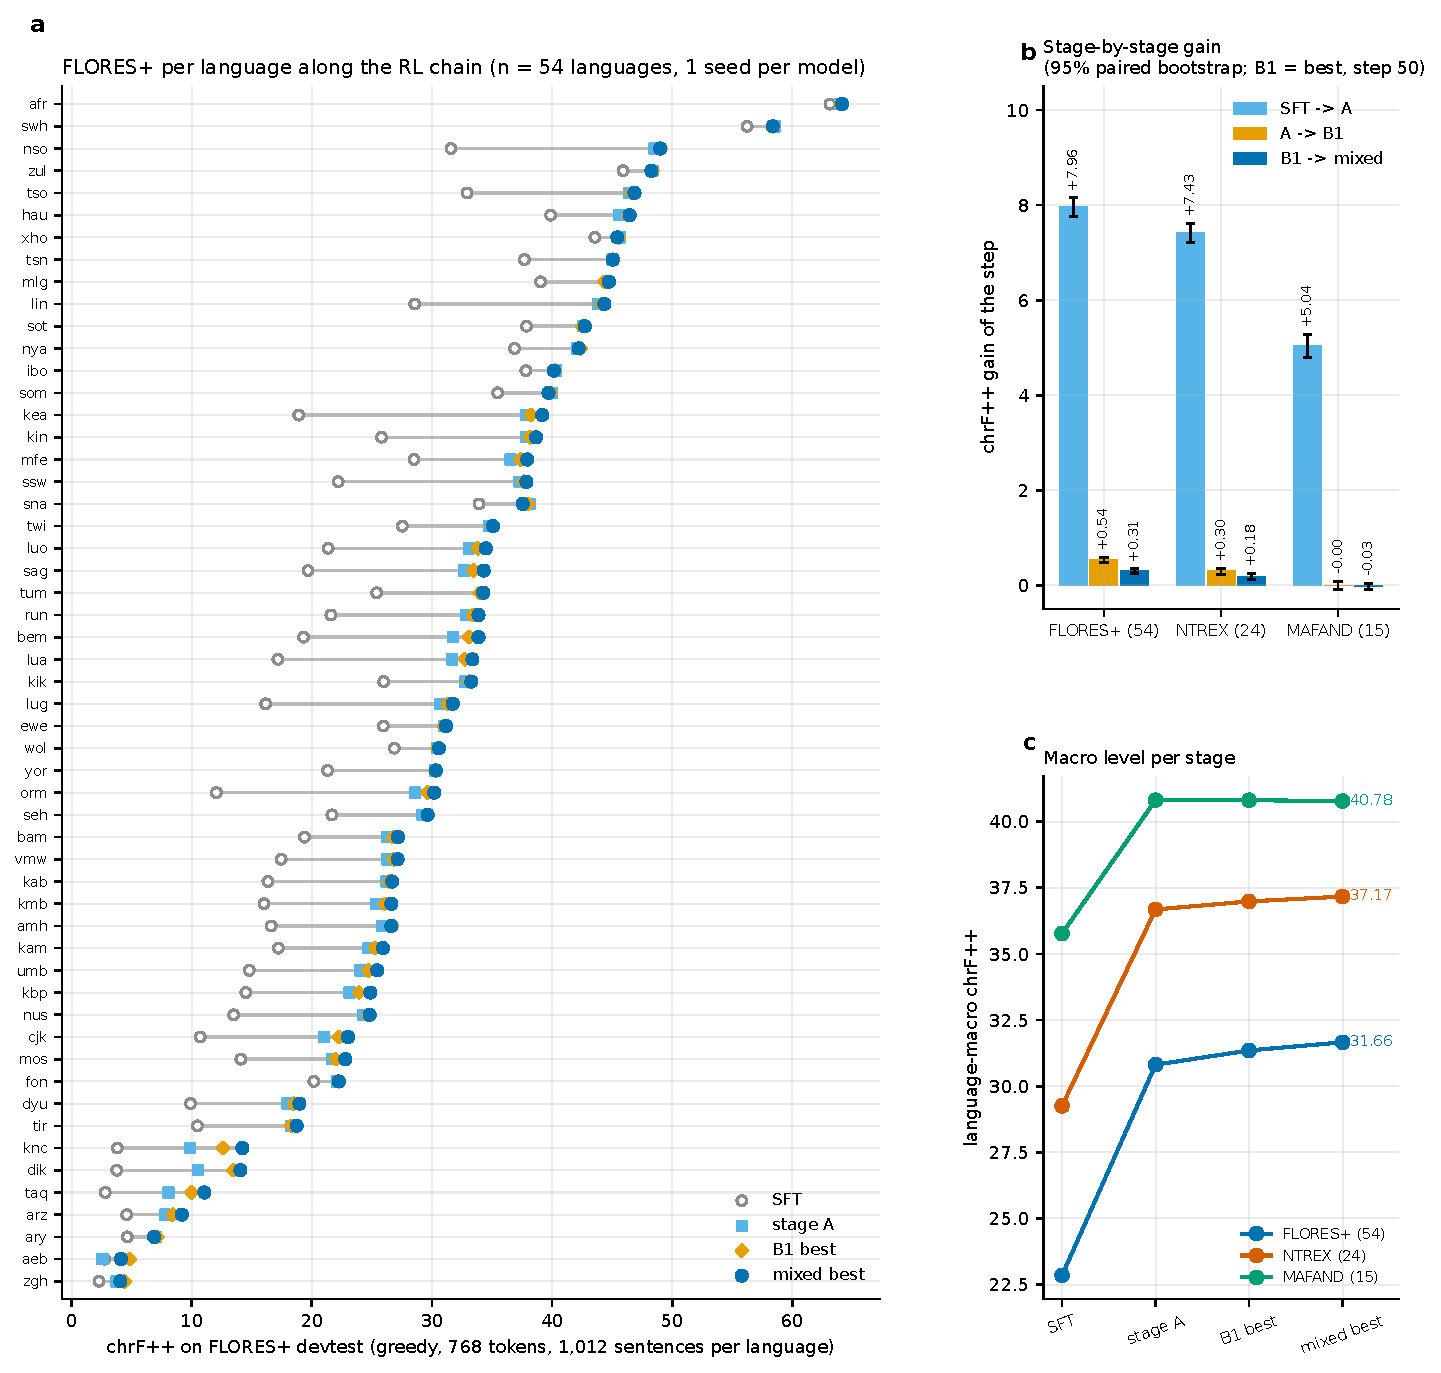
\includegraphics[width=0.95\linewidth]{figures/fig1_flores_per_language.pdf}
\caption{(a) FLORES+ devtest chrF++ per language (n = 54 languages, 1,012 sentences each; greedy, 768 tokens) for the SFT (open circle), RL stage A (square), B1 best (step 50, diamond) and the mixed best (filled circle), sorted by the mixed best; one training seed per model. (b) Gain of each RL step (language macro, 95\% paired bootstrap over sentences, Poisson weights shared across parallel languages) on FLORES+ (54 languages), NTREX (24) and MAFAND (15). (c) Language-macro chrF++ after each stage. Sources: \texttt{reports/\allowbreak{}data/\allowbreak{}eval\_\allowbreak{}weak\_\allowbreak{}group\_\allowbreak{}2026-\allowbreak{}11-\allowbreak{}03/\allowbreak{}results/\allowbreak{}results\_\allowbreak{}\{sft,stageA,b1best,mixedbest\}.\allowbreak{}csv}, \texttt{reports/\allowbreak{}data/\allowbreak{}rl\_\allowbreak{}vs\_\allowbreak{}sft\_\allowbreak{}evidence\_\allowbreak{}2026-\allowbreak{}11-\allowbreak{}04/\allowbreak{}evidence.\allowbreak{}json}.}\label{fig:fig1_flores_per_language}
\end{figure}

Sources: \texttt{reports/data/rl\_vs\_sft\_evidence\_2026-11-04/tables.md} (Tables 6, 7a, 7b) and \texttt{reports/data/nllb\_comparison\_rl\_models\_2026-11-04/table2\_per\_language\_43.csv}. Intervals are 95\% paired bootstrap over sentences (Poisson weights, 1,000 resamples); NLLB columns are published values.

{\scriptsize
\setlength{\tabcolsep}{4pt}
\begin{longtable}{@{}lrrllll@{}}
\caption{RL minus SFT per language on FLORES+ devtest (54 languages, all rows; \chrfpp{}). Finished / loop are the reward's flags; ``paired keeps rows where both models finished and neither loops.}\label{tab:perlang_flores}\\
\toprule
iso & SFT & RL & $\Delta$ all rows [CI] & SFT finished / loop & RL finished / loop & $\Delta$ paired rows [CI] \\
\midrule\endfirsthead
\toprule
iso & SFT & RL & $\Delta$ all rows [CI] & SFT finished / loop & RL finished / loop & $\Delta$ paired rows [CI] \\
\midrule\endhead
\bottomrule\endlastfoot
kea & 18.91 & 39.18 & +20.27 [+18.91, +21.53] & 0.83 / 0.20 & 1.00 / 0.00 & +7.66 [+6.93, +8.42] \\
orm & 12.06 & 30.18 & +18.12 [+17.49, +18.76] & 0.59 / 0.45 & 1.00 / 0.00 & +2.99 [+2.51, +3.50] \\
nso & 31.58 & 49.01 & +17.43 [+15.75, +19.09] & 0.86 / 0.15 & 1.00 / 0.00 & +4.22 [+3.62, +4.91] \\
lua & 17.18 & 33.37 & +16.19 [+15.21, +17.13] & 0.85 / 0.25 & 1.00 / 0.00 & +5.45 [+4.94, +6.03] \\
lin & 28.56 & 44.35 & +15.78 [+14.19, +17.22] & 0.90 / 0.13 & 1.00 / 0.00 & +5.27 [+4.69, +5.84] \\
ssw & 22.20 & 37.86 & +15.66 [+14.46, +16.85] & 0.87 / 0.17 & 1.00 / 0.00 & +5.38 [+4.85, +5.93] \\
lug & 16.17 & 31.73 & +15.57 [+14.66, +16.52] & 0.79 / 0.25 & 1.00 / 0.01 & +5.32 [+4.78, +5.87] \\
sag & 19.68 & 34.31 & +14.62 [+13.64, +15.55] & 0.87 / 0.20 & 1.00 / 0.00 & +5.99 [+5.51, +6.47] \\
bem & 19.31 & 33.88 & +14.56 [+13.63, +15.61] & 0.88 / 0.18 & 1.00 / 0.01 & +7.16 [+6.60, +7.75] \\
tso & 32.92 & 46.86 & +13.93 [+12.43, +15.51] & 0.91 / 0.11 & 1.00 / 0.00 & +4.45 [+3.82, +5.07] \\
luo & 21.36 & 34.49 & +13.13 [+11.91, +14.15] & 0.92 / 0.13 & 1.00 / 0.00 & +6.44 [+5.88, +6.95] \\
kin & 25.81 & 38.66 & +12.86 [+11.66, +14.03] & 0.89 / 0.12 & 1.00 / 0.00 & +5.66 [+5.09, +6.21] \\
cjk & 10.72 & 23.02 & +12.31 [+11.70, +12.89] & 0.71 / 0.31 & 1.00 / 0.01 & +2.13 [+1.86, +2.42] \\
run & 21.59 & 33.88 & +12.29 [+11.21, +13.15] & 0.88 / 0.15 & 1.00 / 0.01 & +5.03 [+4.52, +5.57] \\
nus & 13.49 & 24.82 & +11.32 [+10.73, +11.91] & 0.67 / 0.41 & 1.00 / 0.00 & +1.97 [+1.56, +2.36] \\
umb & 14.80 & 25.46 & +10.66 [+9.77, +11.44] & 0.89 / 0.15 & 1.00 / 0.01 & +4.84 [+4.43, +5.26] \\
kmb & 16.02 & 26.62 & +10.61 [+9.82, +11.37] & 0.88 / 0.23 & 1.00 / 0.00 & +3.93 [+3.56, +4.29] \\
knc & 3.81 & 14.22 & +10.41 [+9.95, +10.88] & 0.46 / 0.94 & 1.00 / 0.48 & +2.49 [+0.82, +3.99] \\
kbp & 14.51 & 24.88 & +10.37 [+9.70, +11.00] & 0.85 / 0.26 & 1.00 / 0.01 & +5.48 [+4.98, +5.94] \\
kab & 16.35 & 26.69 & +10.34 [+9.50, +11.14] & 0.84 / 0.20 & 1.00 / 0.00 & +2.26 [+1.92, +2.61] \\
dik & 3.76 & 14.06 & +10.30 [+9.75, +10.81] & 0.29 / 0.85 & 1.00 / 0.40 & +1.80 [+1.10, +2.60] \\
amh & 16.62 & 26.62 & +10.00 [+9.04, +10.96] & 0.87 / 0.13 & 1.00 / 0.00 & +2.80 [+2.29, +3.29] \\
vmw & 17.45 & 27.14 & +9.69 [+8.92, +10.48] & 0.84 / 0.18 & 1.00 / 0.00 & +2.11 [+1.81, +2.44] \\
mfe & 28.51 & 37.93 & +9.42 [+7.98, +10.94] & 0.94 / 0.07 & 1.00 / 0.01 & +3.91 [+3.43, +4.37] \\
dyu & 9.90 & 18.97 & +9.06 [+8.47, +9.62] & 0.83 / 0.25 & 1.00 / 0.00 & +4.11 [+3.80, +4.44] \\
yor & 21.32 & 30.33 & +9.01 [+7.99, +10.00] & 0.95 / 0.05 & 1.00 / 0.00 & +5.83 [+5.09, +6.56] \\
tum & 25.40 & 34.27 & +8.87 [+7.89, +9.79] & 0.94 / 0.08 & 1.00 / 0.00 & +4.57 [+4.08, +5.06] \\
kam & 17.22 & 25.92 & +8.70 [+7.93, +9.50] & 0.92 / 0.14 & 1.00 / 0.00 & +4.42 [+4.01, +4.83] \\
mos & 14.09 & 22.79 & +8.70 [+8.13, +9.33] & 0.90 / 0.19 & 1.00 / 0.01 & +4.54 [+4.17, +4.89] \\
tir & 10.48 & 18.74 & +8.26 [+7.69, +8.86] & 0.77 / 0.23 & 1.00 / 0.00 & +2.23 [+1.83, +2.66] \\
taq & 2.81 & 11.06 & +8.25 [+7.82, +8.67] & 0.14 / 0.91 & 0.99 / 0.56 & +3.27 [+1.81, +4.58] \\
seh & 21.67 & 29.65 & +7.98 [+7.00, +8.86] & 0.92 / 0.12 & 1.00 / 0.00 & +2.01 [+1.70, +2.33] \\
bam & 19.39 & 27.17 & +7.78 [+6.96, +8.59] & 0.89 / 0.13 & 1.00 / 0.00 & +2.47 [+2.14, +2.80] \\
twi & 27.54 & 35.07 & +7.53 [+6.47, +8.61] & 0.94 / 0.08 & 1.00 / 0.00 & +2.47 [+2.02, +2.92] \\
tsn & 37.69 & 45.05 & +7.36 [+6.18, +8.65] & 0.96 / 0.06 & 1.00 / 0.00 & +2.09 [+1.67, +2.59] \\
kik & 25.98 & 33.28 & +7.30 [+6.39, +8.22] & 0.93 / 0.08 & 1.00 / 0.00 & +3.32 [+2.89, +3.81] \\
hau & 39.88 & 46.46 & +6.58 [+5.09, +8.34] & 0.96 / 0.04 & 1.00 / 0.01 & +0.90 [+0.50, +1.30] \\
mlg & 39.04 & 44.73 & +5.68 [+4.54, +6.77] & 0.97 / 0.03 & 1.00 / 0.00 & +2.03 [+1.59, +2.45] \\
nya & 36.88 & 42.21 & +5.33 [+4.23, +6.54] & 0.97 / 0.04 & 1.00 / 0.00 & +1.82 [+1.41, +2.24] \\
ewe & 25.96 & 31.17 & +5.21 [+4.46, +6.04] & 0.95 / 0.06 & 1.00 / 0.00 & +2.12 [+1.75, +2.51] \\
sot & 37.87 & 42.72 & +4.85 [+3.70, +6.08] & 0.97 / 0.04 & 1.00 / 0.00 & +1.15 [+0.82, +1.50] \\
arz & 4.59 & 9.18 & +4.59 [+4.01, +5.15] & 0.49 / 0.52 & 0.87 / 0.19 & +0.67 [+0.05, +1.25] \\
som & 35.47 & 39.71 & +4.24 [+3.14, +5.34] & 0.97 / 0.03 & 1.00 / 0.00 & +1.38 [+1.02, +1.75] \\
wol & 26.87 & 30.58 & +3.72 [+2.74, +4.63] & 0.97 / 0.03 & 1.00 / 0.00 & +1.14 [+0.82, +1.44] \\
sna & 33.92 & 37.56 & +3.64 [+2.47, +4.85] & 0.97 / 0.04 & 1.00 / 0.00 & +0.26 [\ensuremath{-}0.11, +0.66] \\
zul & 45.91 & 48.27 & +2.36 [+1.56, +3.14] & 0.99 / 0.01 & 1.00 / 0.00 & +1.26 [+0.84, +1.67] \\
ibo & 37.82 & 40.14 & +2.33 [+1.57, +3.08] & 0.98 / 0.02 & 1.00 / 0.00 & +0.88 [+0.53, +1.24] \\
ary & 4.64 & 6.88 & +2.24 [+1.76, +2.74] & 0.54 / 0.48 & 0.97 / 0.11 & \ensuremath{-}3.70 [\ensuremath{-}4.39, \ensuremath{-}3.03] \\
swh & 56.24 & 58.36 & +2.12 [+1.10, +3.38] & 1.00 / 0.01 & 1.00 / 0.00 & +0.88 [+0.45, +1.30] \\
fon & 20.17 & 22.25 & +2.07 [+1.60, +2.55] & 0.98 / 0.04 & 1.00 / 0.00 & +0.77 [+0.56, +0.97] \\
xho & 43.56 & 45.43 & +1.87 [+1.05, +2.80] & 0.99 / 0.01 & 1.00 / 0.00 & +0.67 [+0.28, +1.09] \\
zgh & 2.29 & 4.07 & +1.78 [+1.30, +2.30] & 0.12 / 0.89 & 0.97 / 0.46 & \ensuremath{-}6.69 [\ensuremath{-}9.11, \ensuremath{-}4.34] \\
aeb & 2.75 & 4.12 & +1.36 [+0.96, +1.78] & 0.53 / 0.49 & 0.96 / 0.25 & \ensuremath{-}2.46 [\ensuremath{-}3.19, \ensuremath{-}1.74] \\
afr & 63.13 & 64.13 & +1.01 [+0.53, +1.61] & 1.00 / 0.00 & 1.00 / 0.00 & +0.78 [+0.46, +1.11] \\
\end{longtable}
}

{\scriptsize
\setlength{\tabcolsep}{4pt}
\begin{longtable}{@{}lrrrll@{}}
\caption{RL minus SFT per language on NTREX (clean rows; \chrfpp{} and held-out AfriCOMET).}\label{tab:perlang_ntrex}\\
\toprule
iso & n & SFT chrF++ & RL chrF++ & $\Delta$ all rows [CI] & $\Delta$ AfriCOMET [CI] \\
\midrule\endfirsthead
\toprule
iso & n & SFT chrF++ & RL chrF++ & $\Delta$ all rows [CI] & $\Delta$ AfriCOMET [CI] \\
\midrule\endhead
\bottomrule\endlastfoot
orm & 1992 & 9.63 & 27.33 & +17.70 [+17.16, +18.25] & +0.168 [+0.161, +0.175] \\
ven & 1992 & 21.30 & 38.81 & +17.52 [+16.72, +18.31] & - \\
ssw & 1992 & 21.58 & 38.80 & +17.22 [+16.40, +18.02] & +0.122 [+0.115, +0.130] \\
bem & 1992 & 18.68 & 34.79 & +16.11 [+15.43, +16.84] & +0.111 [+0.105, +0.117] \\
nso & 1992 & 20.14 & 32.73 & +12.60 [+11.83, +13.35] & +0.101 [+0.095, +0.108] \\
tsn & 1992 & 36.97 & 48.71 & +11.74 [+10.68, +12.81] & +0.073 [+0.067, +0.080] \\
kin & 1992 & 26.40 & 37.13 & +10.73 [+9.95, +11.52] & +0.072 [+0.066, +0.078] \\
som & 1992 & 35.84 & 44.23 & +8.39 [+7.44, +9.25] & +0.061 [+0.055, +0.066] \\
yor & 1992 & 23.77 & 32.10 & +8.33 [+7.58, +9.10] & +0.104 [+0.097, +0.110] \\
tir & 1992 & 9.10 & 17.00 & +7.90 [+7.52, +8.25] & +0.144 [+0.136, +0.151] \\
amh & 1992 & 10.58 & 18.05 & +7.46 [+7.00, +7.93] & +0.078 [+0.071, +0.084] \\
ewe & 1992 & 24.28 & 31.58 & +7.30 [+6.64, +8.00] & +0.064 [+0.059, +0.069] \\
hau & 1992 & 42.15 & 48.57 & +6.42 [+5.24, +7.58] & +0.028 [+0.023, +0.034] \\
nya & 1992 & 37.87 & 44.23 & +6.36 [+5.46, +7.34] & +0.025 [+0.020, +0.030] \\
wol & 1992 & 25.29 & 30.37 & +5.08 [+4.34, +5.86] & +0.032 [+0.027, +0.037] \\
sna & 1992 & 34.25 & 39.23 & +4.99 [+4.17, +5.83] & +0.024 [+0.019, +0.029] \\
ibo & 1992 & 39.90 & 44.87 & +4.97 [+4.17, +5.82] & +0.028 [+0.024, +0.032] \\
nde & 1992 & 28.83 & 32.95 & +4.12 [+3.51, +4.74] & - \\
mlg & 1992 & 36.91 & 40.85 & +3.94 [+3.19, +4.74] & +0.026 [+0.021, +0.031] \\
swh & 1992 & 55.18 & 58.73 & +3.55 [+2.55, +4.54] & +0.017 [+0.012, +0.022] \\
zul & 1992 & 40.92 & 43.50 & +2.58 [+1.89, +3.29] & +0.015 [+0.010, +0.019] \\
xho & 1992 & 39.85 & 42.36 & +2.51 [+1.92, +3.16] & +0.013 [+0.009, +0.017] \\
afr & 1992 & 62.42 & 63.92 & +1.50 [+1.00, +2.15] & +0.016 [+0.012, +0.020] \\
shi & 1992 & 0.24 & 1.16 & +0.93 [+0.85, +1.02] & - \\
\end{longtable}
}

{\scriptsize
\setlength{\tabcolsep}{4pt}
\begin{longtable}{@{}lrrrll@{}}
\caption{RL minus SFT per language on MAFAND-MT (clean rows; \chrfpp{} and held-out AfriCOMET).}\label{tab:perlang_mafand}\\
\toprule
iso & n & SFT chrF++ & RL chrF++ & $\Delta$ all rows [CI] & $\Delta$ AfriCOMET [CI] \\
\midrule\endfirsthead
\toprule
iso & n & SFT chrF++ & RL chrF++ & $\Delta$ all rows [CI] & $\Delta$ AfriCOMET [CI] \\
\midrule\endhead
\bottomrule\endlastfoot
lug & 1500 & 26.97 & 39.57 & +12.60 [+11.60, +13.70] & +0.065 [+0.058, +0.071] \\
yor & 1550 & 23.47 & 33.45 & +9.98 [+9.15, +10.70] & +0.127 [+0.119, +0.133] \\
kin & 1005 & 36.51 & 46.41 & +9.90 [+8.70, +11.20] & +0.064 [+0.056, +0.073] \\
luo & 1500 & 22.95 & 32.62 & +9.67 [+8.76, +10.50] & +0.072 [+0.065, +0.079] \\
tsn & 1500 & 43.85 & 53.10 & +9.24 [+7.87, +10.70] & +0.045 [+0.039, +0.052] \\
amh & 1014 & 11.62 & 18.33 & +6.71 [+5.91, +7.46] & +0.061 [+0.052, +0.070] \\
twi & 1500 & 28.58 & 34.14 & +5.56 [+4.75, +6.29] & +0.042 [+0.037, +0.047] \\
nya & 1003 & 38.14 & 40.95 & +2.81 [+1.96, +3.71] & +0.009 [+0.002, +0.015] \\
sna & 1004 & 30.35 & 32.91 & +2.56 [+1.64, +3.39] & +0.018 [+0.011, +0.025] \\
xho & 1001 & 49.76 & 51.78 & +2.02 [+1.06, +2.98] & +0.008 [+0.002, +0.014] \\
ibo & 1458 & 43.55 & 44.89 & +1.34 [+0.43, +2.32] & +0.005 [+0.000, +0.010] \\
swh & 1822 & 50.68 & 51.79 & +1.12 [+0.38, +1.89] & +0.012 [+0.007, +0.017] \\
zul & 998 & 44.50 & 45.58 & +1.08 [+0.49, +1.73] & +0.011 [+0.005, +0.017] \\
hau & 1498 & 32.03 & 32.80 & +0.77 [+0.21, +1.41] & +0.014 [+0.009, +0.019] \\
pcm & 1562 & 53.58 & 53.34 & \ensuremath{-}0.25 [\ensuremath{-}0.69, +0.30] & +0.007 [+0.004, +0.009] \\
\end{longtable}
}

{\scriptsize
\setlength{\tabcolsep}{4pt}
\begin{longtable}{@{}llrrrrl@{}}
\caption{FLORES+ devtest \chrfpp{} on the 43 languages shared with the published NLLB table (our values greedy; NLLB-3.3B published). Yoruba: the published value is anomalously low.}\label{tab:perlang_nllb}\\
\toprule
iso & language & NLLB-3.3B & SFT & RL mixed best & mixed minus NLLB-3.3B & NLLB tertile \\
\midrule\endfirsthead
\toprule
iso & language & NLLB-3.3B & SFT & RL mixed best & mixed minus NLLB-3.3B & NLLB tertile \\
\midrule\endhead
\bottomrule\endlastfoot
yor & Yoruba & 24.90 & 21.32 & 30.33 & +5.43 & tail (15) \\
fon & Fon & 19.30 & 20.17 & 22.25 & +2.95 & tail (15) \\
dyu & Dyula & 16.20 & 9.90 & 18.97 & +2.77 & tail (15) \\
wol & Wolof & 28.10 & 26.87 & 30.58 & +2.48 & tail (15) \\
kam & Kamba & 23.60 & 17.22 & 25.92 & +2.32 & tail (15) \\
kmb & Kimbundu & 24.40 & 16.02 & 26.62 & +2.22 & tail (15) \\
umb & Umbundu & 23.60 & 14.80 & 25.46 & +1.86 & tail (15) \\
afr & Afrikaans & 64.70 & 63.13 & 64.13 & \ensuremath{-}0.57 & high (14) \\
ibo & Igbo & 41.10 & 37.82 & 40.14 & \ensuremath{-}0.96 & mid (14) \\
nso & Sepedi & 50.30 & 31.58 & 49.01 & \ensuremath{-}1.29 & high (14) \\
mos & Mossi & 24.10 & 14.09 & 22.79 & \ensuremath{-}1.31 & tail (15) \\
swh & Swahili & 60.00 & 56.24 & 58.36 & \ensuremath{-}1.64 & high (14) \\
lua & Luba-Kasai & 35.20 & 17.18 & 33.37 & \ensuremath{-}1.83 & tail (15) \\
sag & Sango & 36.50 & 19.68 & 34.31 & \ensuremath{-}2.19 & mid (14) \\
tum & Tumbuka & 36.60 & 25.40 & 34.27 & \ensuremath{-}2.33 & mid (14) \\
nya & Chichewa & 45.30 & 36.88 & 42.21 & \ensuremath{-}3.09 & high (14) \\
som & Somali & 42.80 & 35.47 & 39.71 & \ensuremath{-}3.09 & mid (14) \\
xho & Xhosa & 48.60 & 43.56 & 45.43 & \ensuremath{-}3.17 & high (14) \\
twi & Twi & 38.30 & 27.54 & 35.07 & \ensuremath{-}3.23 & mid (14) \\
tso & Tsonga & 50.20 & 32.92 & 46.86 & \ensuremath{-}3.34 & high (14) \\
tsn & Setswana & 48.60 & 37.69 & 45.05 & \ensuremath{-}3.55 & high (14) \\
bem & Bemba & 37.50 & 19.31 & 33.88 & \ensuremath{-}3.62 & mid (14) \\
lin & Lingala & 48.00 & 28.56 & 44.35 & \ensuremath{-}3.65 & high (14) \\
sot & Sesotho & 46.50 & 37.87 & 42.72 & \ensuremath{-}3.78 & high (14) \\
kik & Kikuyu & 37.30 & 25.98 & 33.28 & \ensuremath{-}4.02 & mid (14) \\
nus & Nuer & 28.90 & 13.49 & 24.82 & \ensuremath{-}4.08 & tail (15) \\
bam & Bambara & 31.40 & 19.39 & 27.17 & \ensuremath{-}4.23 & tail (15) \\
luo & Luo & 39.00 & 21.36 & 34.49 & \ensuremath{-}4.51 & mid (14) \\
kbp & Kabiye & 29.50 & 14.51 & 24.88 & \ensuremath{-}4.62 & tail (15) \\
zul & Zulu & 53.50 & 45.91 & 48.27 & \ensuremath{-}5.23 & high (14) \\
sna & Shona & 42.80 & 33.92 & 37.56 & \ensuremath{-}5.24 & mid (14) \\
kab & Kabyle & 32.00 & 16.35 & 26.69 & \ensuremath{-}5.31 & tail (15) \\
mlg & Malagasy & 50.20 & 39.04 & 44.73 & \ensuremath{-}5.47 & high (14) \\
orm & Oromo & 35.70 & 12.06 & 30.18 & \ensuremath{-}5.52 & tail (15) \\
ssw & Swati & 43.50 & 22.20 & 37.86 & \ensuremath{-}5.64 & mid (14) \\
hau & Hausa & 52.50 & 39.88 & 46.46 & \ensuremath{-}6.04 & high (14) \\
tir & Tigrinya & 24.80 & 10.48 & 18.74 & \ensuremath{-}6.06 & tail (15) \\
lug & Luganda & 38.50 & 16.17 & 31.73 & \ensuremath{-}6.77 & mid (14) \\
ewe & Ewe & 38.20 & 25.96 & 31.17 & \ensuremath{-}7.03 & mid (14) \\
run & Kirundi & 41.90 & 21.59 & 33.88 & \ensuremath{-}8.02 & mid (14) \\
kea & Kabuverdianu & 47.90 & 18.91 & 39.18 & \ensuremath{-}8.72 & high (14) \\
kin & Kinyarwanda & 48.40 & 25.81 & 38.66 & \ensuremath{-}9.74 & high (14) \\
amh & Amharic & 37.90 & 16.62 & 26.62 & \ensuremath{-}11.28 & mid (14) \\
\end{longtable}
}

\section{Limitations: full list}\label{app:limits}

The numbered list of Appendix~\ref{app:limits} is a compressed version of this one.

\begin{enumerate}
\item \textbf{Single training seed} for every model and stage; all intervals are test-sentence bootstrap (1,000 resamples; Poisson weights shared across parallel languages for the RL-versus-SFT claims), and some are over languages only (NLLB, family analysis). Evaluation noise of the dev macro is sd 0.09 to 0.10 chrF++; training-run variation was measured only for the stage-A recipe at 100 steps on 20 languages with one pair of extra seeds (E-04: 0.06 chrF++ [\ensuremath{-}0.02, +0.14] between the two; Appendix~\ref{app:split}); seeds of later stages, of the science and long-document stages and of the SFT are not available (a second SFT seed is impractical: stage B alone is 44.8 A100-hours). The mixed step (+0.31 on FLORES+; +0.07 on the 20 languages of the seed study) and per-language differences under about 0.5 chrF++ (pcm, hau, ibo) cannot be separated from seed noise.
\end{enumerate}
% GATE E-01 E-03
\begin{enumerate}
\item \textbf{The matched-compute control is one run.} E-03 (Section~\ref{sec:control}) has one seed, one learning rate (the pre-registered probe's best of three), one data mix (50\% replay + 50\% TranslatePsy for 19 languages, with NLLB-3.3B targets) and \textbf{one evaluated budget point (6,000 steps)}: the stage-A-matched (3,100) and mixed-best-matched (4,800) checkpoints exist but were not evaluated, at the authors' request. Its registered verdict is ``inconclusive'' and was not changed. The decode-time loop-guard control (E-01) is reported in Section~\ref{sec:rlsft}, with the caveats that its best setting was the grid edge and that a stronger penalty was explored only on dev.
\item \textbf{No human judgement of system outputs} (E-10: not run; it needs native-speaker annotators, which the authors cannot commission, and no LLM-judge substitute was validated). All evidence is automatic; the neural checks are of one family, and AfriCOMET has a length/entity bias (shown next to chrF++, never alone). One reference per sentence.
\item \textbf{Reward-family overlap.} Finished, loop and language-ID rates are optimised by construction; SSA-COMET-QE (the AfriScience-MT headline) is a checkpoint of the reward's family; chrF++ is partly optimised through the consensus utility and, for 5 + 7 languages, through the NLLB and human-reference terms. The reward's own loop flag undercounts degeneration by 1.77 on FLORES+ (Section~\ref{sec:degen}), and the independent detector shares the repetition concept and is blind to non-repetitive failure.
\item \textbf{Ablations are limited} (E-11): three arms (no features, no reference domain, no beam guide) at 100 steps of the b64 recipe, one run per arm, sharing a 40-step prefix with seed 2, 20 languages, one pair of seeds as the noise yardstick; the KL-guard arm was not run (the guard never fired); dynamic sampling and the std floor alone, the reward components other than the reference term, and the later stages were not ablated; the mid-run changes of Appendix~\ref{app:disc} mean the stages are not a clean single design.
\end{enumerate}

\begin{enumerate}
\item \textbf{Metric choices changed after the fact for the science analysis}: the headline moved from reference-based SSA-COMET-MTL to reference-free SSA-COMET-QE after a calibration on released sentence-level runs only; the paper's own checkpoint is unverified.
\item \textbf{Engine and decoding.} The bf16 engine parity gate was not met (9.6\% identical outputs vLLM bf16 against HF bf16; chrF++ 36.22, 36.80, 38.18 on 240 sentences); E-09 shows the engines agree in fp32 (98.8\% and 97.1\% identical outputs for the SFT and the RL model), so the gate failure is bf16 rounding. E-09b: the SFT in fp32 on the full set differs from bf16 by \ensuremath{-}0.04 chrF++ [\ensuremath{-}0.13, +0.07] over 93 cells, so the bf16 headline does not overstate the RL gain; the earlier +0.24 to +1.81 range is superseded. Not done: the RL model in fp32 and AfriCOMET scoring of the fp32 SFT run. All headline numbers are vLLM 0.32.0 bf16 greedy at 768 tokens. Beam-4 and MBR-16 were measured at 768 tokens (E-02) on the SFT and the RL model only, on 20 languages $\times$ 200 sentences, with one SFT and one RL checkpoint, chrF++ as the MBR utility (metric-matched), a primary beam definition amended after a smoke test and before any score (stop at 4 ended hypotheses), and a second beam rule that gives a different sign for the RL model; the earlier 256-token beam numbers used a loop that ran past the end token and are not comparable.
\item \textbf{Language coverage.} 51 of 125 registry languages have no reference test and are unscored; many weak languages rest on one benchmark of 48 to 1,012 sentences; the family analysis covers 54 languages. The model fails on Arabic dialects, Tamazight, Dinka, Tamasheq and Kanuri, and RL increases English output there.
\item \textbf{Comparisons.} The old-versus-385M comparison (E-13, same harness, rows clean for both generations) is still a composite of data, steps, tokenizer layout and reward, with FLORES+ reduced to 4.7\% of its rows; the NLLB comparison uses FLORES-200 published numbers against FLORES+, beam against greedy and language-level intervals; AfriqueLLM numbers come from a different few-shot harness; bidirectional aggregates are not compared.
\item \textbf{Documents.} 28 papers per language (168 documents; the document intervals of the long-document RL are bootstrap over documents and reflect paper sampling only; the other document tables have no bootstrap); whole-document decoding was tested at 4,096 new tokens and remains unusable after the long-document RL (72 to 73\% loops); COMET encoders read 512 tokens, so only 4-sentence-window values are document scores; the 385M RL stages trained on prompts of at most 256 source tokens before the long-document RL.
\item \textbf{Cost and scale.} One 385M model and one language registry; A100 hours as in Section~\ref{sec:method}; no scaling claim.
\item \textbf{Unresolved and unevaluated items.} B1 final (step 135) was evaluated after the fact (E-20, \texttt{reports/\allowbreak{}e20\_\allowbreak{}b1\_\allowbreak{}final\_\allowbreak{}2026-\allowbreak{}11-\allowbreak{}04.\allowbreak{}md}): it equals B1 best (step 50) within noise (+0.01 chrF++ [\ensuremath{-}0.02, +0.04], AfriCOMET +0.0004 over 93 cells; the 85 later steps changed nothing measurable), and the mixed stage is +0.26 [+0.22, +0.30] chrF++ over B1 final on FLORES+; the NLLB-data ablation was not run [E-17]; sentence-paired comparison with NLLB on the full devtest was not run [E-06b].
\item \textbf{Not run:} human evaluation (needs native-speaker annotators); the packed-shard contamination scans, the content check of A0 against g0, the embedding and MT round-trip paraphrase scans and the source of the other 34 dev-train-half languages (need the data box); the NLLB-data ablation (skipped by the authors); beam widths other than 4, length penalties and the 54-language decoding run; a science SFT at alpha 1.0 followed by RL, a second seed of E-14 and a long-document RL from the E-14 model.
\end{enumerate}

\section{Disclosures: full statement}\label{app:disc}

Rule: data and signals that were actually used are stated, including those that are non-commercial or NLLB-derived. \texttt{DISCLOSURES.\allowbreak{}md} is the source of this section and holds the full tables. 
% src: DISCLOSURES sections 1-6; claims IDs L1-L5, CT1-CT13, CTL1-CTL6

\subsection{Training data and licences}


\begin{itemize}
\item \textbf{NLLB-derived share of the SFT.} NLLB-mined bitext (OPUS-NLLB, 43 languages, 13.46 M rows, plus a Fulah NLLB-mined set of 0.45 M rows) is \textbf{14.4\% of the 3.990 B stage-B pack tokens} (13.3\% of the 4.109 B executed; 10.84\% of the 5.043 B tokens drawn in the whole SFT); adding NLLB-Seed (tzm) and the aligned part of the Aya collection (NLLB-3.3B outputs; 169 M tokens in 12 languages) gives \textbf{18.7\%} (746 M tokens; executed 17.2\%; 14.36\% of the whole SFT); adding the machine-translated Tumbuka instruction sets (system not stated, possibly NLLB) gives \textbf{22.8\%} (909 M tokens; 17.86\% of the whole SFT). By rows, 13.91 M of 42.31 M stage-B translation pairs (32.9\%) are NLLB-mined. A0 contains none of the three. The authors allowed NLLB-mined rows with a per-language cap of 150k, ODC-BY with special attribution. NLLB models and outputs carry CC-BY-NC terms and the authors cannot use NLLB for production translation; a licence statement must accompany any release of the 385M weights. Not counted and needing a legal decision: the \texttt{*\_\allowbreak{}mt560} OPUS sets (69\% of the main pair output of the clean rebuild, 16.2 M of 23.4 M pairs, mostly Jehovah's Witnesses and Bible text, licence unknown, labelled NLLB-derived by an old converter docstring); \texttt{African-\allowbreak{}Languages-\allowbreak{}Lab/\allowbreak{}multi-\allowbreak{}open} (3,748,964 pairs, ``license: other''); AfroLingu-MT (gated, authors' exception); other machine-translated instruction sets with unstated systems (\texttt{african\_\allowbreak{}ultrachat}, \texttt{kiya\_\allowbreak{}sft}, \texttt{alpaca\_\allowbreak{}*}, \texttt{amharic\_\allowbreak{}*}); all four families are in the instruction pack stream (\texttt{packed\_\allowbreak{}instr}: every source of the instruction intake except \texttt{muri\_\allowbreak{}it}, 4,190,976 samples, 1.232 B tokens; \texttt{reports/\allowbreak{}intake2\_\allowbreak{}instr\_\allowbreak{}packs\_\allowbreak{}2026-\allowbreak{}11-\allowbreak{}01.\allowbreak{}md}); \texttt{african\_\allowbreak{}ultrachat} is UltraChat machine-translated into 11 languages, \texttt{alpaca\_\allowbreak{}*} (twi, swh, zul, wol, som) are translated Alpaca sets, \texttt{amharic\_\allowbreak{}*} and \texttt{kiya\_\allowbreak{}sft} (om, yo, sw, am rows) are machine-translated sets, and the translation system is not stated in the dataset cards or in the intake records; the packs carry no source field, so the tokens of each source drawn in stage B are not recorded. 
% src: NLLBLINK Licence-disclosure figure; HYG X10; REBUILD section 9; DISCLOSURES 1.1
\item \textbf{Unspecified-licence sources} in the main output: KwekuAinoo/eng\_twi 551,358; sentence-transformers/parallel-sentences-opus-100 210,479; UBC-NLP/AfroLingu-MT 207,796; cibfaye/wolof-english-bible 11,415; webfaq\_v2; bambara\_lm\_qa (381k, 83\% of Bambara instruction rows). Religious text dominates many low-resource languages (28 of the 81 RL languages are religious-only in the post-editor selection); the Efik NT sheet (7,936 verse pairs) has unconfirmed provenance and licence.
\item \textbf{IbomMT} is CC-BY-NC-4.0: a disclosed non-commercial exception in the SFT (once) and a human-reference source of the RL reference domain (efi, ibb).
\item \textbf{Quarantined and not used:} \texttt{yigagilbert/\allowbreak{}synthetic-\allowbreak{}parallel-\allowbreak{}external}, \texttt{fiifinketia/\allowbreak{}pristine-\allowbreak{}twi-\allowbreak{}english}, \texttt{muri-\allowbreak{}it}, the Aya parallel pairs.
\item \textbf{Gemma base model:} \texttt{google/\allowbreak{}gemma-\allowbreak{}3-\allowbreak{}270m-\allowbreak{}it}; the Gemma terms of use apply to the derived weights; pretraining text is unknown, so exposure of benchmarks through pretraining cannot be excluded.
\item \textbf{FLORES+ dev train half} (440 ids; 23,706 of 23,760 rows found in the audit) is in the SFT on purpose; the held-out half (557 ids) is protected.
\end{itemize}

\subsection{RL prompts and reward-side data}


\begin{itemize}
\item General prompts: FineWeb-Edu (ODC-By) and Wikipedia (CC BY-SA). News prompts (30\% of the draw): BBC News 2017-2025 (\texttt{RealTimeData/\allowbreak{}bbc\_\allowbreak{}news\_\allowbreak{}alltime}, \textbf{no licence declared, BBC copyright}), \texttt{permutans/\allowbreak{}c4-\allowbreak{}bbc-\allowbreak{}news} (ODC-By label inherited from C4, BBC copyright applies), Wikinews (CC BY 2.5), Global Voices (CC BY 3.0 per the sister card), Wikivoyage (CC BY-SA 4.0; 188 prompts drawn in stage A) and \texttt{SetFit/\allowbreak{}bbc-\allowbreak{}news} (37 pool rows, none drawn, licence not recorded). The prompts are RL \textbf{input} text only; the source is never a training target.
\item Seven new-language prompt files of stage A (\texttt{tll mfe guw lub crs zne lue}) had not been filtered; stage A drew 6 flagged prompts of 28,120 (0.021\%), 6 of 1,345 for those languages, source side only. B1 was restarted from its step-20 checkpoint with the filtered pool.
\item Reference domain (stage A from step 41, B1, mixed, science RL): human pairs from AfriScience-MT \textbf{train} (Apache-2.0; amh hau lug nso yor zul) and IbomMT train (CC-BY-NC-4.0; efi, ibb), anchors for 7 languages only. Test papers are in no pool. 0.9\% of the AfriScience train rows have their African-language sentence in the A0 pair data (Appendix~\ref{app:contam}).
\item \textbf{NLLB-3.3B pseudo-references (CC-BY-NC) are a reward signal} for kea kbp nus bam kab (weight 0.25, max 0.35), reward only; no NLLB text is a training target in RL.
\item Reward models: \texttt{masakhane/\allowbreak{}africomet-\allowbreak{}qe-\allowbreak{}stl-\allowbreak{}1.\allowbreak{}1}, \texttt{McGill-\allowbreak{}NLP/\allowbreak{}ssa-\allowbreak{}comet-\allowbreak{}mtl}; held-out monitor \texttt{masakhane/\allowbreak{}africomet-\allowbreak{}stl-\allowbreak{}1.\allowbreak{}1} (apache-2.0 verified); GlotLID language guard. Licences as declared on the Hub (read 2026-11-05): \texttt{McGill-\allowbreak{}NLP/\allowbreak{}ssa-\allowbreak{}comet-\allowbreak{}mtl} and \texttt{ssa-\allowbreak{}comet-\allowbreak{}qe} apache-2.0; \texttt{masakhane/\allowbreak{}africomet-\allowbreak{}qe-\allowbreak{}stl-\allowbreak{}1.\allowbreak{}1} apache-2.0; \texttt{cis-\allowbreak{}lmu/\allowbreak{}glotlid} \texttt{license: other} with \texttt{license\_\allowbreak{}name: apache-\allowbreak{}2.\allowbreak{}0-\allowbreak{}plus-\allowbreak{}notices} (card: Apache License 2.0 plus notices).
\item Science stages: science RL prompts \texttt{clean\_\allowbreak{}sci\_\allowbreak{}v2} (PMC, arXiv CC BY/CC0, AfriScience-MT train English); \textbf{LibreTexts was excluded} from the science RL (licence conflict CC BY against CC BY-NC-SA, 10,257 prompts). \textbf{LibreTexts is not absent from the long-document RL pool}: 3,428 \texttt{common-\allowbreak{}pile/\allowbreak{}libretexts} rows (17.8\% of \texttt{science\_\allowbreak{}b2048}). The rows were removed before the stage started; the long-document RL did not use them. The E-14 run (science RL started from the mixed best) used the same pool and reward as the executed science RL. Science SFT: AfriScience-MT train (Apache-2.0; 28,750 windows) plus replay cut from the general SFT shards (so the NLLB, Aya and Tumbuka shares apply to the replay); 54 further catalogue candidates were scanned and none used.
\end{itemize}

\subsection{TranslatePsy: used only in a research control}


\texttt{qvac/\allowbreak{}TranslatePsy-\allowbreak{}AfriSLM-\allowbreak{}Synthetic-\allowbreak{}Mix} (Gritta et al.; CC-BY-NC-4.0; targets are \texttt{facebook/\allowbreak{}nllb-\allowbreak{}200-\allowbreak{}3.\allowbreak{}3B} translations of MADLAD-400 sentences, filtered by AfriCOMET, SSA-COMET and MetricX) was authorised by the authors on 2026-11-04 \textbf{for the matched-compute continued-SFT control (E-03) only}. Its English-to-X rows (19 languages: afr amh hau ibo kin lin lug mlg nya orm sna som sot swh tsn wol xho yor zul) enter that control run, scanned against the protected index (any hit on either side removed; 0.67\% of the 950,000-row sample); \textbf{no TranslatePsy row is in the SFT, any RL stage, the science or long-document stages, or any released weight.} The control checkpoints are research artefacts (CC-BY-NC-4.0 and NLLB terms), are not pushed to any public repository and are not used in production. The comparison RL against control must state two things: the TranslatePsy quality filters are the reward family of the RL, so neural metrics favour the control while chrF and chrF++ do not; and TranslatePsy targets are NLLB-3.3B-like, so a good control result partly means ``distilling NLLB''. Status: run (preparation \texttt{reports/\allowbreak{}sft\_\allowbreak{}control\_\allowbreak{}prep\_\allowbreak{}2026-\allowbreak{}11-\allowbreak{}04.\allowbreak{}md}; execution record and result \texttt{reports/\allowbreak{}e03\_\allowbreak{}sft\_\allowbreak{}control\_\allowbreak{}2026-\allowbreak{}11-\allowbreak{}05.\allowbreak{}md}): 277,900 pairs per language for the 19 languages (5.28 M pairs, 96,138 packs, each seen once) after removing every row with a hit against the protected index; the control checkpoint is a research artefact under CC-BY-NC-4.0 and the NLLB terms, kept on the authors' storage, never released and never used in a released model. The comparison states that the TranslatePsy filters are the reward family of the RL, so AfriCOMET and SSA-COMET-QE favour the control, and that its targets are NLLB-3.3B outputs (Section~\ref{sec:control}).  
% GATE E-03
% src: CTLP sections 1, 5, 7; DISCLOSURES 1.1, 4

\subsection{Analysis decisions and data-audit facts}


\begin{itemize}
\item The 385M SFT text contains no benchmark sentence of 3 or more words; one- and two-word strings, numerals and names occur (NTREX 0.25\%, MAFAND 0.47\%, SmolSent 0.12\%, GlotStoryBook 0.44\% of rows); phrase-level exposure is in Appendix~\ref{app:contam}.
\item The RL dev set is a FLORES+ dev subset (720 sentences, 18 languages). The weak-language choice used devtest-derived per-language tables (selection on a test set).
\item Benchmarks were evaluated many times; checkpoint choice used only the 720-sentence dev set. The science alpha rule was written before the headline metric was fixed; the headline then changed from SSA-COMET-MTL (reference-based) to SSA-COMET-QE after the calibration. The post-hoc RL-versus-SFT decomposition ran after the results were known.
\item The earlier 270M pipeline (not the clean 385M rerun) trained on text that held the English side of 95\% of FLORES+ devtest; the old 270M models; their numbers appear only on their clean rows (48 sentences per language on FLORES+) and are descriptive; the earlier 270M work's FLORES+ results are not reused.
\item FLORES+ and FLORES-200 references differ in places; the NLLB comparison uses published FLORES-200 numbers.
\end{itemize}

\subsection{Process disclosures}


\begin{itemize}
\item \textbf{Gates overridden by the authors.} The RL preflight gate failed (gradient norm 3.40 > 3.0, greedy loop 0.109 > 0.02, greedy finished 0.906 < 0.97) and was overridden; the stage-A gate failed (max KL 0.169 > 0.15, three KL-guard cuts, greedy loop 0.016 > 0.01) and B1 was started on the authors' instruction.
\item \textbf{Mid-run changes.} Stage A was stopped at step 40 and resumed with the four features; B1 was restarted at its step-20 checkpoint (filtered prompt pool, reference domain, oversample 1.0, KL guard 0.25) and again at step 40 (MBR guide, dev early stop); the mixed stage was restarted at its step-20 checkpoint with the patch-3 monitor, and the authors loosened the hacking alarm (chrF++ 0.3 $\to$ 0.75; AfriCOMET 0.005 $\to$ 0.03). Stage A's KL guard cut the learning rate three times and it never recovered.
\item \textbf{Start checkpoints.} Mixed started from B1 best (step 50), not B1 final; B1 final exists on the Hub and was evaluated after the fact (E-20): it equals B1 best within noise (+0.01 chrF++ [\ensuremath{-}0.02, +0.04] over 93 cells). The weak-group run never produced a \texttt{best/\allowbreak{}} checkpoint; its final (step 85) was evaluated. The \texttt{masakhane/\allowbreak{}africomet-\allowbreak{}stl-\allowbreak{}1.\allowbreak{}1} monitor influenced early stopping in the mixed stage and later (never a reward).
\item \textbf{Incident.} The mixed stage was auto-started once by a process outside the launch agent, stopped within a minute without a step, and relaunched from B1 best. A first science-SFT pipeline pass wrote an empty alpha and launched the science RL with an invalid model path, which stopped itself at start. The GPU idled for about 2 h 10 min between stage A and B1. The E-14 run (science RL from the mixed best) had one CUDA out-of-memory in the COMET reward worker at about step 38; the launcher lowered the micro-batch from 12,288 to 6,144 tokens and resumed from the step-20 checkpoint, so steps 21 to 38 were replayed (same prompt schedule, vLLM sampling not bit-reproducible); \texttt{metrics.\allowbreak{}jsonl} holds two records for those steps and the later one is used.
\item \textbf{Science RL length.} The science-RL yaml names 150 steps a hard cap, but the trainer's extension rule raised the cap to 190 steps at step 120 while dev metrics were still improving; the run then stopped on a dev plateau at step 150 and, after a 10-step wind-down, executed 160 steps (\texttt{summary.\allowbreak{}json}). The long-document RL has the extension rule off.
\item \textbf{Checkpoint storage.} Stage checkpoints were written to RAM-backed \texttt{/\allowbreak{}dev/\allowbreak{}shm}; weights are in anonymised repositories, optimiser states are not.
\item \textbf{Evaluation-only tool under a non-commercial licence:} the NLLB-218 language-ID model (cc-by-nc-4.0) was used for measurement only.
\item \textbf{Compute.} A100 80 GB (vast.ai) for SFT stage B (44.8 h), RL (8.66 GPU-h for A + B1 + mixed), evaluation and the science stage; smaller boxes for data preparation and the post-editor. GPU-hours by component, estimated from logged durations, are in Appendix (compute table): the sized components sum to about 94 A100-hours; A0, SFT-1 and several evaluation passes are not sized; no cost figure is reported.
\end{itemize}

\subsection{Intended use and risks}


Outputs are machine translations of unverified quality for languages without any human evaluation, with documented failure modes: Arabic dialects, Tamazight, Dinka, Tamasheq and Kanuri are not usable (chrF++ 2 to 14 after RL), RL increases English output there, and the model should be used sentence by sentence, not on whole documents. Religious text dominates the data of many low-resource languages, which may shift register and vocabulary toward it. The model must not be presented as a replacement for NLLB-class systems: it is 3.26 chrF++ below NLLB-3.3B on 43 shared languages. The authors' use case is production translation; the licences of NLLB and TranslatePsy prevent using those systems there, which is why we state exactly where NLLB-derived text and signals entered this model.

\section{Reproducibility statement}\label{app:repro}

\begin{itemize}
\item \textbf{Code and configs.} \texttt{gemma\_\allowbreak{}mt/\allowbreak{}} (trainer \texttt{train\_\allowbreak{}sft.\allowbreak{}py}, RL \texttt{gemma\_\allowbreak{}mt/\allowbreak{}rl/\allowbreak{}}, evaluation scripts); SFT configs \texttt{reports/\allowbreak{}data/\allowbreak{}e23\_\allowbreak{}hygiene\_\allowbreak{}2026-\allowbreak{}11-\allowbreak{}04/\allowbreak{}sft\_\allowbreak{}configs/\allowbreak{}}; RL configs \texttt{.\allowbreak{}.\allowbreak{}.\allowbreak{}/\allowbreak{}rl\_\allowbreak{}configs/\allowbreak{}} (note: the archived stage-A \texttt{config.\allowbreak{}json} is the resumed configuration); reports and per-language tables under \texttt{reports/\allowbreak{}} and \texttt{reports/\allowbreak{}data/\allowbreak{}} as keyed in \texttt{CLAIMS\_\allowbreak{}LEDGER.\allowbreak{}md}; analysis scripts for every new section in \texttt{reports/\allowbreak{}data/\allowbreak{}\{nllb\_\allowbreak{}comparison\_\allowbreak{}rl\_\allowbreak{}models,family\_\allowbreak{}script\_\allowbreak{}resource\_\allowbreak{}analysis,degeneration\_\allowbreak{}audit\_\allowbreak{}independent,stage\_\allowbreak{}A\_\allowbreak{}feature\_\allowbreak{}split,contamination\_\allowbreak{}followups\_\allowbreak{}385m,e23\_\allowbreak{}hygiene\}\_\allowbreak{}2026-\allowbreak{}11-\allowbreak{}04/\allowbreak{}}.
\item \textbf{Seeds and hyper-parameters.} Seed 1234 throughout; SFT: Muon, peak 5e-5 (SFT-1, shard 1) and 3e-5 (shards 2-6) with cosine floors 50\% (SFT-1), 80\% (shards 1-5) and 10\% (shard 6), 131,072 tokens per step (Section~\ref{sec:method}); RL stages A to mixed: Muon, 2e-6, group 16, KL 0.05 (reference = each stage's start model), guard 0.15/0.25, temperature 1.0; \textbf{science RL: Muon, 1.0e-6, KL 0.1, group 16, guide 0.25, 160 steps executed (yaml cap 150, extended to 190, stopped by dev plateau); long-document RL: Muon, 1.0e-6, KL 0.1, group 8, no guide, 80 steps $\times$ 32 prompts} (Table~\ref{tab:stagecfg_full}); science SFT AdamW 3e-6, alpha 0.5. The science-RL yaml is in \texttt{reports/\allowbreak{}data/\allowbreak{}rl\_\allowbreak{}configs\_\allowbreak{}as\_\allowbreak{}executed\_\allowbreak{}2026-\allowbreak{}11-\allowbreak{}04/\allowbreak{}sci\_\allowbreak{}rl\_\allowbreak{}F\_\allowbreak{}final.\allowbreak{}yaml}.
\item \textbf{Hardware and software.} One A100 80 GB; vLLM 0.32.0 bf16 greedy, 768 new tokens, for every headline number. Outputs are not bit-identical across engines (9.6\% identical between vLLM bf16 and HF bf16 on 240 sentences); a reader reproducing with another engine should expect small, unsystematic differences (240 sentences, HF bf16 minus vLLM bf16: +0.54 [\ensuremath{-}0.67, +1.79] chrF++ for the SFT and \ensuremath{-}0.23 [\ensuremath{-}0.73, +0.23] for the RL model; the SFT in fp32 against bf16 on the full set: \ensuremath{-}0.04 [\ensuremath{-}0.13, +0.07] over 93 cells, E-09b, which supersedes the earlier +0.24 [\ensuremath{-}0.07, +0.55] on 4,000 sentences and +1.81 on 240 sentences). sacreBLEU 2.6.0 and the chrF++/spBLEU settings are given in Section~\ref{sec:eval}; the full signature strings are not recorded; exact commands per table are in the archived scripts named in the ledger.
\end{itemize}

\begin{itemize}\item \textbf{Weights and branches.} \anonreal{All checkpoints named in the paper (SFT final, RL stages, science and long-document stages, seed, ablation and E-14 runs) are in anonymised repositories, released on acceptance; the control checkpoint is not published (CC-BY-NC data).}{RL repository \url{https://huggingface.co/AletheiaAING/gemma-0.4B-translate-rl}: branch \texttt{main} (mixed best, the final general RL model), \texttt{latest}, \texttt{stage-a-b64} (stage A step 200), \texttt{stage-a-final} (step 400), \texttt{stage-b1-b256} (B1 best, step 50), \texttt{stage-b1-final} (step 135), \texttt{stage-g-weak-latest}, \texttt{science-sft}, \texttt{science-sft-alpha1}, \texttt{science-rl}, \texttt{science-rl-latest}, \texttt{science-rl-final}, \texttt{long-rl}, \texttt{long-rl-latest} (long-document RL checkpoints) and tag \texttt{rl-step-50}. SFT final: \url{https://huggingface.co/AletheiaAING/gemma-0.4B-translate-sft} (branch \texttt{main}, step 32,853). Experiment weights: \url{https://huggingface.co/AletheiaAING/gemma-0.4B-translate-rl-experiments}, branches \texttt{e04-seed2-step100}, \texttt{e04-seed3-step100}, \texttt{e04-a\_base-step100}, \texttt{e04-c\_noref-step100}, \texttt{e04-d\_noguide-step100}, \texttt{e14-science-rl-only-final}. The control checkpoint of E-03 is not published (CC-BY-NC data). No licence field or model card is declared on these repositories \ownerdecision{confirm release licence}.} Run configs, logs, per-sentence outputs and scripts of E-02, E-04, E-11 and E-14 are in the research archive and the reports directory named in the ledger.\end{itemize}

\begin{itemize}
\item \textbf{Data.} The decontaminated SFT and RL prompt data and the protected index (\texttt{protected-\allowbreak{}2026-\allowbreak{}10-\allowbreak{}28.\allowbreak{}3}) are in anonymised storage named in the reports and released on acceptance; the NC and unspecified-licence parts cannot be redistributed as they are (Appendix~\ref{app:disc}); TranslatePsy rows are not released (Appendix~\ref{app:disc}). The state, prompts, eval and reports repositories were private at the last check (Hub API 2026-11-04). [OWNER: which parts of the data are released.]
\item \textbf{Long-document RL incident.} The stage took 7.7 h of wall-clock time (10:03 to 17:44 UTC), of which about 4.5 h were a crash loop: the trainer stopped (ENOSPC, root disk full) at the first step-25 evaluation and Hub-staging save and was restarted 18 times by the supervisor, each time resuming from \texttt{last/\allowbreak{}} at step 20 and repeating steps 21 to 25; the staging directories were real directories on the root disk instead of symlinks to \texttt{/\allowbreak{}dev/\allowbreak{}shm}. Fixed at 15:35 UTC; the model path of the 80 steps is otherwise the planned one (one seed). About 3.2 h were productive. The repeated step-20-to-25 segments are visible as repeated step-25 evaluations in the metrics log (Figure of the training records). 
% src: reports/eval_long_document_rl_385m_2026-11-04.md section 0 'Costs and caveats'; reports/rl_long_document_plan_2026-11-04.md section 8; reports/overnight_log_2026-11-04.md 11:10-15:35
\item \textbf{Not reproducible from what is stored:} stage-A steps 1-40 hyper-parameters except through the stage report; B1 final's evaluation; per-sentence NLLB hypotheses on the full devtest; the training seed spread; the SFT with another seed (stage B alone is 44.8 A100-hours).
\end{itemize}

\section{Prompt format and data statement}\label{app:format}

\paragraph{Prompt format.} Every translation request is the fixed prompt \texttt{Translate the text to \{language\}:  \{english\}} (two spaces after the colon) inside the Gemma 3 chat template; the model answers \texttt{<tag> \{translation\}<end\_of\_turn>} with the single-token tag of the target language; the loss covers the answer only (Section~\ref{sec:method}). \textbf{RL prompts} are English windows of consecutive sentences from FineWeb-Edu and Wikipedia (70\%) and from news (30\%), filtered against the protected index; 81 languages with higher draw weights for the 29 weakest (Section~\ref{sec:method}).

\paragraph{Data statement.} Training data are English-to-African-language pairs and instruction data in 125 languages from the sources listed in Appendix~\ref{app:disc} and Appendix~\ref{app:disc}; many low-resource languages are dominated by religious text; stage B includes NLLB-mined, Aya-aligned and machine-translated instruction data; evaluation data are human references of FLORES+ devtest, NTREX-128, MAFAND-MT, SmolSent, SALT, GlotStoryBook, IbomMT, FLORES-MOZ and AfriScience-MT. No personal data was collected by us; no human subjects were involved; no human evaluation was run.

\section{Responsible NLP checklist: items filled from the paper}\label{app:rnlp}

% Filled only from paper.md / ledger / report facts. Compute: GPU-hours only, estimated from logged durations (no cost figures).
\begin{itemize}
\item \textbf{Scientific artefacts used and licences.} Base model: Gemma-3-270m-it (Gemma terms of use apply to the derived weights). Reward and monitor models, as declared on the Hub (read 2026-11-05): \texttt{McGill-NLP/ssa-comet-mtl} and \texttt{ssa-comet-qe}, \texttt{masakhane/africomet-qe-stl-1.1} and \texttt{africomet-stl-1.1}: apache-2.0; GlotLID (\texttt{cis-lmu/glotlid}): \texttt{license: other}, \texttt{license\_name: apache-2.0-plus-notices}. Training and reward-side data and their licences are listed in Ethical considerations and Appendix~\ref{app:disc}: NLLB-mined and NLLB-derived data (CC-BY-NC terms), IbomMT (CC-BY-NC-4.0), AfriScience-MT train (Apache-2.0), FineWeb-Edu (ODC-By), Wikipedia (CC BY-SA), several sources with unspecified licences; TranslatePsy (CC-BY-NC-4.0, NLLB-3.3B targets) only in the research control. Evaluation uses the public benchmarks named in Section~\ref{sec:eval}; the NLLB-218 language-ID model (CC-BY-NC) was used for measurement only. Release licence of the weights: the Hub repositories declare none \ownerdecision{confirm release licence}.
\item \textbf{Parameters and compute.} 385,144,448 parameters; one A100 80\,GB at a time. Table~\ref{tab:compute} gives A100-hours per component, \emph{estimated from logged durations} (training seconds from the run summaries, or the logged start and end times of the job); no cost figure is reported. The sized components add up to about 94 A100-hours, a lower bound. \textbf{Not sized} (no duration in any report): the A0 stage (5,625 steps) and SFT-1 (1,500 steps); E-01 (guard grid and guarded full evaluations); E-09 and E-09b (the fp32 generation ran 17:46 to 18:38 UTC beside another job at a 0.15 GPU share); E-13 and E-20; the SSA-COMET scoring of E-05; the full evaluation passes of every stage (122,585 rows each) and the AfriScience and document evaluations; data preparation and scoring boxes; aborted runs and the compute of the earlier 270M models.
\item \textbf{Number of runs and seeds.} One training run per model and stage (seed 1234); two extra seeds (20261105, 20261106) of the stage-A recipe at 100 steps; three ablation arms, one run each; the control and the E-14 run are one run each. No multiple-run statistics beyond that pair; test-sentence bootstrap intervals elsewhere.
\item \textbf{Hyper-parameters and selection.} Appendix~\ref{app:hyper} (all SFT and RL settings, per-shard schedules, reward and features). Checkpoints were selected on a 720-sentence FLORES+ dev subset; the decode-time guard setting by a rule fixed in advance on the SFT dev grid.
\item \textbf{Evaluation.} Metrics defined in Section~\ref{sec:eval}; sacreBLEU 2.6.0 (from the install log of the evaluation machine; the full signature strings were not recorded), chrF++ = \texttt{CHRF(word\_order=2)} with the defaults, spBLEU = BLEU with \texttt{tokenize=flores200}, NFC-normalised hypotheses and references; vLLM 0.32.0, bf16, greedy, 768 new tokens; intervals are 95\% paired bootstrap, 1,000 resamples (language bootstrap, 10,000 resamples, for NLLB). Exact commands per table are in the archived scripts named in the ledger.
\item \textbf{Human subjects and annotators.} None were involved; no human judgement of system outputs was collected; no personal data was collected by us.
\item \textbf{Code, data and checkpoints.} \anonreal{Anonymised for review; released on acceptance, subject to the licence limits above.}{See the links in Ethical considerations and the branch list in the reproducibility statement, subject to the licence limits above.} NLLB-derived and non-commercial parts cannot be redistributed as they are, and TranslatePsy rows are not released \ownerdecision{which parts of the data are released}.
\end{itemize}

\begin{table}[h]
\centering\small
\caption{A100-hours by component, estimated from logged durations (lower bound; unsized components are listed above).}\label{tab:compute}
\begin{tabular}{@{}lrl@{}}
\toprule
component & A100-h & basis\\
\midrule
SFT stage B (31,353 steps) & 44.8 & 5.14 s per step\\
RL stage A, B1, mixed (400 + 135 + 60 steps) & 8.66 & 15,920 + 10,479 + 4,786 s\\
weak-group RL (85 steps) & 2.1 & 7,642 s\\
science SFT (283 steps) & 0.3 & 17 min\\
science RL (160 steps) & 4.8 & 17,153 s\\
long-document RL (80 steps) & 7.7 & wall-clock 10:03--17:44, of which about 4.5 h crash loop\\
E-03 control (6,000 steps and two probes) & 10.5 & GPU session 9.75 h, evaluation 0.55 h, SSA-COMET pass 0.2 h\\
E-02 beam-4 and MBR-16 & 2.6 & logged GPU time\\
E-04 two seed runs and their evaluations & 3.2 & wall-clock 08:51--12:05\\
E-11 three ablation arms and evaluations & 2.9 & 36 + 54 + 42 min of training, 3 $\times$ about 15 min of evaluation\\
E-14 science RL without science SFT & 6.0 & training 15:18--20:17, evaluation about 1 h\\
\midrule
sized components, total & about 94 & lower bound\\
\bottomrule
\end{tabular}
\end{table}


\end{document}
